%
% OSU Thesis and Dissertation LaTeX File
%
% Master file: master.tex
%
% This is the file that links all of the parts of the MS thesis or
% PhD dissertation together and invokes the OSU official document
% style.
%
% The OSU Astronomy Department has modified the Graduate School's
% LaTeX templates to allow use of AASTeX-style markup, making for
% easy conversion of journal papers into the proper dissertation style.
% It also provides access to the AASTeX table formats, so that you 
% don't have to retype all of your tables (this is a good thing).
%
% It also fixes some bugs in the Graduate School's style files.  These
% could be real bugs or could simply be a different reference version
% of TeX, we're not sure.
%
% Based on modifications made by Andrew Stephens and Rick Pogge.
%
% Annotations below describe how to use this.  There are some examples
% of the various pages in this directory, see especially:
%
%	title_srh.tex   - title page template for the Senior Honors thesis
%	title_ms.tex    - title page template for the MS thesis
%	title_phd.tex   - title page template for the PhD dissertation
%	abstract.tex    - abstract template
%	dedication.tex  - dedication template
%	acknowledge.tex - acknowledgements template
%	vita.tex        - Vita template
%       biblio.tex      - Bibliography template
%
% To process, type
%
%    latex master.tex
% 
% repeating this until all warnings about references and cross-references
% are resolved (usually 3-4 times).
%
% To process the dissertation text for conversion to PDF (using either
% Adobe Distiller or ps2pdf):
%
%    dvips -t letter -Ppdf -o master.ps master.dvi
%
% The Graduate School requires that all dissertations and theses produced
% after Autumn Quarter 2002 be submitted electronically as PDF files.
%
% The ``dotex'' script has been provided to handle all of the basic
% dirty work of processing the .tex file into .ps
%	
% Modification History: 
%   2002 January 1 - hooks for thesis (MS) and dissertation (PhD) following
%                    the 2001/2002 Graduate School Handbook [rwp]
%   2002 May 28 - hooks for pdf conversion and bookmarks following the
%                 new Graduate School e-submission requirements [rwp]
%
%   2004 Jun 18 - Of course some of the rules changed, this tries to
%                 accommodate them.  Who thinks these things up? [rwp]
%
%   2013 May 14 - Been a while, but some rules changed again, mostly minor
%                 but pay particular attention to the order of chapters,
%                 bibliography, and appendices. [rwp]
%
%   2014 Jul 9  - Routine check against graduate school rules, and
%                 additions to documentclass options (oneside, hidelinks)
%                 to address issues for electronic dissertations [rwp]
%
%   2016 May 30 - Added the amsmath and tocloft packages. The latter allows
%                 printing the LoF and LoT with the words "Figure" or "Table"
%                 before each number, respetively. [rwp]
%
%%%%%%%%%%%%%%%%%%%%%%%%%%%%%%%%%%%%%%%%%%%%%%%%%%%%%%%%%%%%%%%%%%%%%%%%%%%

% Formatting Information: don't touch unless you have to...

% *** LOAD PACKAGES IN THIS ORDER... ***
%
% If you take it upon yourself to change the order, *bad* things *WILL* 
% happen.  Wicked bad spooky voodoo kinds of things.  Trust us...
%

% The documentclass options in [] setup formatting parameters that
% address grad school and electronic dissertation formatting requirements.
% 
%    12pt = body text base font size is 12pt
%    fleqn = left side alignment of displayed math equations
%    oneside = avoids rogue blank pages that sometimes get created
%              between parts or chapters because book default is 2-sided
%    hidelinks = removes the ugly "blue boxes" around active hyperlinks
%

\documentclass[12pt,fleqn,oneside,hidelinks]{book}
% \usepackage{setspace}
% \usepackage{aaspp4}	% For compatibility with aastex'isms
% \usepackage{epsfig}	% for importing Encapsulated PostScript figures
% JCZ 150319 !!! commented this out to try out my bibliography appraoch, using mktex
%\usepackage{biblatex}	% Bibliography style
%\usepackage{deluxetable}
%\usepackage{mnras}
% \usepackage{natbib}
\usepackage[style=authoryear-comp, natbib=true, backend=bibtex]{biblatex}
\usepackage[explicit, compact]{titlesec}
\usepackage[titles]{tocloft} % ToC, LoF, LoF typesetting
\bibliography{main}
% \renewcommand*\finalnamedelim{\addspace\&\space}
% \renewcommand*\nameyeardelim{\addspace}
% \AtBeginBibliography{\renewcommand*\finalnamedelim{\addcomma\space}}
% \DeclareFieldFormat{journaltitle}{#1}
% \DeclareFieldFormat{pages}{#1}
% \DeclareNameAlias{sortname}{family-given}
% \DeclareBibliographyDriver{article}{%
% 	\printnames{author}%
% 	\addcomma\addspace%
% 	\printfield{year}%
% 	\addcomma\addspace%
% 	\printfield{journaltitle}%
% 	\addcomma\addspace%
% 	\printfield{volume}%
% 	\addcomma\addspace%
% 	\printfield{pages}%
% }

%\usepackage{natbib,amsmath,multirow,tabularx}
%\usepackage{bk12e}	% A modified bk12.sty to work with LaTeX2e
\usepackage{osuthesis}	% OSU thesis format
\usepackage{setspace}
\usepackage{lscape}	% support for embedded landscape pages (e.g., tables)
\usepackage{graphicx}   % support for includegraphics et al.
\usepackage{amsmath}
\usepackage{amssymb}
\usepackage{mathtools}
\usepackage{apptools}
\usepackage{afterpage}
%\usepackage{refcheck}	% Uncomment to check references, usually unnecessary

% User's \usepackage imports:
% \usepackage{amssymb}
\usepackage{color}
% \usepackage{lscape}
\usepackage{subfiles}
\usepackage{ragged2e}
\usepackage{tabularx}
\usepackage{bm}
\usepackage[toc, title, page]{appendix}

% Any new commands we need - this file contains all the current
% AASTeX markup so you don't have to import it yourself.

% \input{newcommands.tex}

\newcommand{\mc}{\textsc{emcee}}
\newcommand{\vice}{\textsc{VICE}}
\newcommand{\python}{\textsc{python}}
\newcommand{\ah}{\ensuremath{\text{[}\alpha\text{/H]}}}
\newcommand{\oh}{\ensuremath{\text{[O/H]}}}
\newcommand{\nh}{\ensuremath{\text{[N/H]}}}
\newcommand{\feh}{\ensuremath{\text{[Fe/H]}}}
\newcommand{\afe}{\ensuremath{\text{[$\alpha$/Fe]}}}
\newcommand{\ofe}{\ensuremath{\text{[O/Fe]}}}
\newcommand{\no}{\ensuremath{\text{[N/O]}}}
\newcommand{\ohno}{\no-\oh}
\newcommand{\Ctwelve}{\ensuremath{^{12}\text{C}}}
\newcommand{\Cthirteen}{\ensuremath{^{13}\text{C}}}
\newcommand{\Cfourteen}{\ensuremath{^{14}\text{C}}}
\newcommand{\Nthirteen}{\ensuremath{^{13}\text{N}}}
\newcommand{\Nfourteen}{\ensuremath{^{14}\text{N}}}
\newcommand{\Nfifteen}{\ensuremath{^{15}\text{N}}}
\newcommand{\Ofifteen}{\ensuremath{^{15}\text{O}}}
\newcommand{\Osixteen}{\ensuremath{^{16}\text{O}}}
\newcommand{\logage}{\ensuremath{\log_{10}\text{(age)}}}
\newcommand{\ddfrac}[2]{\frac{\displaystyle{#1}}{\displaystyle{#2}}}
\newcommand{\refp}[1]{(\ref{#1})}
\newcommand{\subcc}{\ensuremath{_\text{cc}}}
\newcommand{\ycc}[1]{\ensuremath{y_\text{#1}^\text{CC}}}
\newcommand{\yia}[1]{\ensuremath{y_\text{#1}^\text{Ia}}}
\newcommand{\yagb}[1]{\ensuremath{y_\text{#1}^\text{AGB}}}
\newcommand{\yacc}{\ensuremath{y_\alpha^\text{CC}}}
\newcommand{\yfecc}{\ensuremath{y_\text{Fe}^\text{CC}}}
\newcommand{\yfeia}{\ensuremath{y_\text{Fe}^\text{Ia}}}
\newcommand{\script}[1]{\ensuremath{\mathcal{#1}}}
\newcommand{\scinote}[2]{\ensuremath{#1\times10^{#2}}}
\newcommand{\erf}{\ensuremath{\text{erf}}}
\newcommand{\msun}{\ensuremath{\text{M}_\odot}}
\newcommand{\mstar}{\ensuremath{\text{M}_\star}}
\newcommand{\persqkpc}{\ensuremath{\text{kpc}^{-2}}}
\newcommand{\rgal}{\ensuremath{R_\text{gal}}}
\newcommand{\absz}{\ensuremath{\left|z\right|}}
\newcommand{\gaia}{\textit{Gaia}}
\newcommand{\um}{\textsc{UniverseMachine}}
\newcommand{\hsim}{\texttt{h277}}
\newcommand{\flow}{\ensuremath{\text{flow}}}
\newcommand{\eq}{\ensuremath{\text{eq}}}
\newcommand{\grad}[1]{\ensuremath{\nabla\text{[#1/H]}}}
\newcommand{\timescale}[1]{\ensuremath{\tau_\text{#1}}}
% \newcommand{\overequalsign}[1]{\stackrel{\mathclap{\mbox{\ensuremath{#1}}}}{=}}

% nitrogen chapter -> yield model short-hand names
\defcitealias{Cristallo2011}{C11}
\defcitealias{Cristallo2015}{C15}
\defcitealias{Karakas2010}{K10}
\defcitealias{Karakas2016}{KL16}
\defcitealias{Karakas2018}{K18}
\defcitealias{Ventura2013}{V13}
\newcommand{\cristallo}{\citetalias{Cristallo2011}+\citetalias{Cristallo2015}}
\newcommand{\karakasten}{\citetalias{Karakas2010}}
\newcommand{\karakas}{\citetalias{Karakas2016}+\citetalias{Karakas2018}}
\newcommand{\ventura}{\citetalias{Ventura2013}}



% Put your custom macro definitions here (DO NOT HACK newcommands.tex)
% These are just examples.  Please be sparing, as the more macros you define, 
% the higher the risk of weird formatting errors later.
% for bam

% Uncomment \normalmargins below to produce a draft copy of the
% dissertation with "normal" 1-inch margins rather than the
% Grad School's "big" margins.

%\normalmargins

%
% THIS \usepackage MUST ALWAYS BE ***LAST***
%
% The \usepackage[]{} line below is required to ensure that the document
% you generate satisfies the Grad School's electronic submission rules.  
% It provides for the correct translation into PDF when you run the 
% PostScript output from dvips through the Acrobat distiller or ps2pdf
% to create the required PDF version.
%

% \usepackage[ps2pdf,bookmarks=true,breaklinks=true]{hyperref}
\usepackage[bookmarks=true,breaklinks=true]{hyperref}
% \hypersetup{draft} % turns off citation links
\hypersetup{
	colorlinks = true,
	linkcolor = blue,
	citecolor = blue,
	urlcolor = blue
}

%%
%% *** DON'T TOUCH THESE!!! ***
%%
%% These are the required margins.  They must be defined here, as some of
%% the packages you loaded above with \usepackage will try to change them
%% (sweet, huh?).  Do not mess with these or your thesis/dissertation will
%% be unacceptable to the Graduate School (and you don't need that...)
%%

% \setlength{\topmargin}{0.00in}
% \setlength{\headheight}{0in}
% \setlength{\headsep}{0in}
% \setlength{\oddsidemargin}{0.55in}
% \setlength{\evensidemargin}{0.55in}
% \setlength{\textwidth}{6.0in}  %% avoids overrun in PS/PDF generation
% \setlength{\textheight}{8.5in}
% \setlength{\footskip}{0.4in}
% \setlength{\parskip}{0.15in}
% \setlength{\parindent}{5ex}

% uncomment these lines if you want LaTeX to shut up about vboxes and hboxes
\hbadness=10000 % default = 1000
\vbadness=10000 % default = 1000

% Some bibliography punctuations that are required.  These affect the
% appearance of \citep, \citet, and associated citation macros.  It's
% all fairly arcane, so just leave it alone, OK? 
% JCZ 150319 !!! commented this out too
% \bibpunct[,]{(}{)}{;}{a}{}{,}

% All done, now you may begin the document

\begin{document}
\emergencystretch 3em

%%%%%%%%%%%%%%%%%%%%%%%%%%%%%%%%%%%%%%%%%%%%%%%%%%%%%%%%%%%%%%%%%%%%%%%%%%%
%
% Front Matter
%
% In Order:
%	Title Page (in required format, see title_ms.tex/_phd/_srh)
%	Abstract (see abstract.tex)
%	Dedication (see dedication.tex)
%	Acknowledgements (see acknowledge.tex)
%	Vita (see vita.tex)
%	Table of Contents
%	List of Tables
%	List of Figures
%
% Pages in this section are given lower-case roman numerals (ii, iii, etc.)
%

% Title page in required Grad School Format.  
% Use title_ms.tex, title_phd.tex, or title_srh.tex as required.

\thispagestyle{empty} % no page number on first page

% \input{title_phd.tex}  % PhD Dissertation
%\input{title_ms.tex}   % MS Thesis
%\input{title_srh.tex}  % Senior Honors Thesis

%%%%%%%%%%%%%%%%%%%%%%%%%%%%%%%%%%%%%%%%%%%%%%%%%%%%%%%%%%%%%%%%%%%%%%%%%%%
%
% Title Page for Doctor of Philosophy (PhD) Degree
%
% Follows OSU Graduate School document prepration guidlines.  See
%
%   www.gradsch.osu.edu/guidelines.html
%
% to obtain copies of the relevant documents.
%
% Updated: 
%   2014 May 6 - routine maintenance based on recent Graduate
%                school formatting documents [rpw/osu]
%
%%%%%%%%%%%%%%%%%%%%%%%%%%%%%%%%%%%%%%%%%%%%%%%%%%%%%%%%%%%%%%%%%%%%%%%%%%%

\begin{titlepage}

%
% Title of the PhD Dissertation goes here.  Large font, regular font,
% mixed case preferred
%


\begin{center}
\begin{singlespace}
\vspace*{1.3cm}
{\Large
% Simultaneous Constraints on Galaxy Evolution and Stellar Nucleosynthesis
From Dwarfs to Spirals: Archaeology of Galaxies with Implications for Stellar
Nucleosynthesis
}
\end{singlespace}

%
% The following sections are REQUIRED TEXT
%
% Do not modify this section under any circumstances
%
% Note:
%   PhD = Dissertation
%    MS = Thesis 
%
% PhDs do not write a Thesis. Ever. Never ever.
%

\vspace*{1.5cm}

DISSERTATION\\
\vspace*{1.5cm}
\begin{singlespace}
Presented in Partial Fulfillment of the Requirements for
the Degree Doctor of Philosophy in the Graduate School of The Ohio 
State University\\
\end{singlespace}
\vspace*{1.0cm}


%
% Enter your Full Legal Name here.  
%
% Make sure the year of your dissertation is correct!
%
\begin{doublespace}
By
\\
James William Johnson
\\
% \vspace*{0.1cm}
Graduate Program in Astronomy
\\
\vspace*{1.0cm}
The Ohio State University\\
2023\\

%
% Dissertation Committee
%
\vspace*{2.5cm}
Dissertation Committee:\\
%
% Enter the names/titles of your exam committee here, starting with your
% adviser.  There is space for 3 names maximum as per Grad School rules.
%
% Make sure there are no blank lines below!
%
% And, yes, it *is* spelled "Advisor", not "Adviser"
%'
Professor David H. Weinberg, Advisor
\\
Professor Jennifer A. Johnson
\\
Professor Christopher S. Kochanek


%
% New page, also un-numbered, with the copyright statement.
%
% Fill in your Full Legal Name and the year, as shown
%
\newpage

\thispagestyle{empty} % no page number on first page

\vspace*{5.0cm}
Copyright by
\\
James William Johnson
\\
2023
\end{doublespace}
\end{center}

%
% all done!
%
\end{titlepage}


% 
\documentclass[ms.tex]{subfiles}
\begin{document}

\begin{abstract}
We derive empirical constraints on the nucleosynthetic yields of nitrogen by
incorporating N enrichment into our previously developed and empirically tuned
multi-zone galactic chemical evolution model.
We adopt a metallicity-independent (``primary'') N yield from massive stars and
a metallicity-dependent (``secondary'') N yield from AGB stars.
In our model, galactic radial zones do not evolve along the observed
[N/O]-[O/H] relation, but first increase in [O/H] at roughly constant [N/O],
then move upward in [N/O] via secondary N production.
By~$t\approx5$ Gyr, the model approaches an equilibrium [N/O]-[O/H] relation,
which traces the radial oxygen gradient.
% {\color{red}
Reproducing the [N/O]-[O/H] trend observed in extra-galactic systems constrains
the ratio of IMF-averaged N yields to the IMF-averaged O yield of core collapse
supernovae.  We find good agreement if we adopt
$\ycc{N}/\ycc{O}=0.024$ and $y_\text{N}^\text{AGB}/\ycc{O} = 0.062(Z/Z_\odot)$.
For the theoretical AGB yields we consider, simple stellar populations 
release half their N after only $\sim$250 Myr.
Our model reproduces the [N/O]-[O/H] relation found for Milky Way stars
in the APOGEE survey, and it reproduces (though imperfectly) the trends of
stellar [N/O] with age and [O/Fe].
The metallicity-dependent yield plays the dominant role in shaping the gas-phase
[N/O]-[O/H] relation, but the AGB time-delay is required to match the stellar
age and [O/Fe] trends.
If we add~$\sim$40\% oscillations to the star formation rate, the model
reproduces the scatter in the gas phase [N/O]-[O/H] relation observed 
in external galaxies by MaNGA.
We discuss implications of our results for theoretical models of N production
by massive stars and AGB stars.
% }
\end{abstract}

\end{document}


%%%%%%%%%%%%%%%%%%%%%%%%%%%%%%%%%%%%%%%%%%%%%%%%%%%%%%%%%%%%%%%%%%%%%%%%%%%
%
% Dedication Template
%
% Dedication of the thesis/dissertation follows the abstract on a
% separate page.
% 
% The brief, one-line dedication text is centered on the page
%
% Updated:
%   2014 May 6 - annual review of grad school formating rules [rwp/osu]
%
%---------------------------------------------------------------------------

\vspace*{1cm}

\addcontentsline{toc}{chapter}{Dedication}

\begin{center}
{\large Dedication}

% one-line dedication here
To family, friends, and loved ones

\end{center}

\clearpage

%%%%%%%%%%%%%%%%%%%%%%%%%%%%%%%%%%%%%%%%%%%%%%%%%%%%%%%%%%%%%%%%%%%%%%%%%%%
%
% Acknowledgments Template
%
% The acknowledgments section follows the dedication.  Can be as long or
% short as you wish (``Brevity is the soul of wit''), but generally should
% be a brief, sincere, and professional acknowledgement of everyone who
% played a role in your dissertation (advisor, faculty, fellow students,
% observatory support, etc.).  Funding agencies and fellowships should
% be acknowledged as well.
%
% Updated:
%   2014 May 6 - annual review of grad school formating rules [rwp/osu]
%
%---------------------------------------------------------------------------

\documentclass[main.tex]{subfiles}
\begin{document}

\vspace*{1cm}
\addcontentsline{toc}{chapter}{Acknowledgments}
\begin{center}
{\large Acknowledgments}
\end{center}

\begin{doublespace}

% Where do I even begin?
My gratitude for the support I have received along the journey to this
dissertation is simply too big for words.
I will try nonetheless.
\par
I will start by thanking the Ohio State Department of Astronomy for providing
me with the opportunity of a lifetime.
A number of my colleagues and mentors have described this department as
``greater than the sum of its parts.''
I can think of no better single-phrase explanation, though it takes the
privilege of existing in this environment to understand just how truly special
it is.
I can only assume that there is some kind of magic behind how one group of
people can be so scientifically empowering and so personally welcoming at the
same time.
\par
I would especially like to thank my dissertation advisor, David Weinberg, for
being everything I could have hoped for in a mentor and more.
Aside from the unfathomable amount of scientific and professional instruction
you have provided me with, I learned the qualities that make one a fantastic
mentor by experiencing them firsthand.
I would also like to thank Jennifer Johnson and Christopher Kochanek for being
wonderful and brilliant advisors who I am honored to have worked with.
I hope that one day I will provide the same quality of mentorship for my
students as I have received from my committee.
Thank you to many more collaborators, advisors, and co-authors who have taught
me so much, especially Charlie Conroy, Jon Bird, Fiorenzo Vincenzo, Emily
Griffith, Ryan Cooke, Annika Peter, and Kris Stanek.
Thank you to many other members of the deparment who have been a delight to
work with, particularly Wayne Schlingman, Adam Leroy, and Todd Thompson.
\par
I would like to thank my classmates for making my graduate school experience so
personally rewarding.
For pizza on Friday nights, drinks at the barcade, and cherished memories,
thank you Patrick, Tharindu, Emily,
Romy, Rachel, Grace, Dom, Alison, Liam, Jack, Jack, Ari, Josh, Ness, Amanda,
Miqaela, Anusha, Lyra, Kiersten, Sarah, Samson, Caprice, Elvira, Tawny, Deb,
Tyler, Matthias, Becca, Joy, Sebastian, Sinclaire, Michael, Karina, and yet
many more.
I'd like to thank friends from outside of the Astronomy Department for all of
the smiles and laughs over the years, especially Maxim, Trenton, Nick, Kendyll,
Falcon, Andrea, Grant, Victor, Cat, Daniel, Elena, Adrian, and Elline.
\par
I'd like to thank my family for their unending support.
My parents, for teaching me ambition and disipline and giving me the resources
to succeed.
For your diligence and sacrifices to ensure that I had opportunities to pursue
my dreams.
My sisters, for their guidance, encouragement, advice, and comfort at every
step of the way.
\par
Finally, to Lauren.
I have been chasing the stars my entire adult life, and they led me to you.
You give a man who cannot help but endlessly stargaze a reason to keep an
eye on Earth.
Thank you for your love and support through thick and thin.
I cannot wait to see what the next chapter of our lives has in store for us.








% Where do I even begin? A list of people I'd like to thank for their unfailing
% support:
% \begin{itemize}

% 	\item My committee

% 	\item Other collaborators and advisors

% 	\item My family

% 	\item Lauren

% 	\item Friends and classmates

% \end{itemize}

\end{doublespace}

\end{document}


% %%%%%%%%%%%%%%%%%%%%%%%%%%%%%%%%%%%%%%%%%%%%%%%%%%%%%%%%%%%%%%%%%%%%%%%%%%%
%
% Vita & Publications Template
%
% The Graduate School requires a Vita in slightly different format than
% the usual Astronomy CV.  The example below is extracted from various
% sources.
%
% The publications list is numbered, and the citation format is DIFFERENT 
% than used in journal articles.  The format lists all authors, the full
% title of the paper, then the journal citation, as follows:
%
%	1. A. Author, B. Author, and C. Author, ``The Full Paper Title'',
%	AJ, 114, 107, (1997)
%	\\
%       \\
%	2. ....
%	\\
%
% Note the double "\\"'s on separate lines used between each entry in the 
% publications list.  This is done to make double-space single-spaced items.  
% Not pretty but it works.
%
% WARNING: NO BLANK LINES ANYWHERE IN THE LIST OF PAPERS!!!
%
%
% Updated:
%   2014 May 6 - annual review of grad school formating rules [rwp/osu]
%
%%%%%%%%%%%%%%%%%%%%%%%%%%%%%%%%%%%%%%%%%%%%%%%%%%%%%%%%%%%%%%%%%%%%%%%%%%%%

\documentclass[main.tex]{subfiles}
\begin{document}

\vspace*{1cm}
\addcontentsline{toc}{chapter}{Vita}

% Vita - copy lines as required, note how to make blank entries

\begin{center}
{\large Vita}
\end{center}

\begin{singlespace}
\vspace*{0.3cm}
\noindent
\makebox[7cm][l]{May 4, 1995 \dotfill}%
\makebox[5cm][l]{Born -- Iowa City, Iowa}%
\linebreak
\linebreak
\makebox[7cm][l]{2017 \dotfill}%
\makebox[5cm][l]{B.A., Physics \& Astronomy}%
\linebreak
\makebox[7cm][l]{\null}%
\makebox[5cm][l]{Vanderbilt University, Nashville, TN, USA}%
\linebreak
\linebreak
\makebox[7cm][l]{2017 \dotfill}%
\makebox[5cm][l]{Larry Ross Cathey Award}%
\linebreak
\makebox[7cm][l]{\null}%
\makebox[5cm][l]{Vanderbilt Universtiy, Nashville, TN, USA}%
\linebreak
\linebreak
\makebox[7cm][l]{2017 -- 2018 \dotfill}%
\makebox[5cm][l]{University Fellowship}%
\linebreak
\makebox[7cm][l]{\null}%
\makebox[5cm][l]{The Ohio State University, Columbus, OH, USA}%
\linebreak
\linebreak
\makebox[7cm][l]{2018 -- 2022 \dotfill}%
\makebox[5cm][l]{Graduate Research and Teaching Associate}%
\linebreak
\makebox[7cm][l]{\null}%
\makebox[5cm][l]{The Ohio State University, Columbus, OH, USA}
\linebreak
\linebreak
\makebox[7cm][l]{2019 \dotfill}%
\makebox[5cm][l]{M.S., Astronomy}
\linebreak
\makebox[7cm][l]{\null}%
\makebox[5cm][l]{The Ohio State University, Columbus, OH, USA}
\linebreak
\linebreak
\makebox[7cm][l]{2022 \dotfill}%
\makebox[5cm][l]{Ann S. Tuttle Graduate Student Paper Prize}%
\linebreak
\makebox[7cm][l]{\null}%
\makebox[5cm][l]{The Ohio State University, Columbus, OH, USA}%
\linebreak
\linebreak
\makebox[7cm][l]{2022 -- 2023 \dotfill}%
\makebox[5cm][l]{Presidential Fellowship}%
\linebreak
\makebox[7cm][l]{\null}%
\makebox[5cm][l]{The Ohio State University, Columbus, OH, USA}%


%% Publications (see above for format, examples given below).  Note that
%% Grad School standard format for literatur citations differs slightly
%% from our usual journal style, and since the Grad School frankly doesn't 
%% care how we do it in our journals, do it their way or else.

\begin{center}
{\large Publications}
\end{center}

\begin{flushleft}
\textbf{Research Publications}
\end{flushleft}

\begin{enumerate}

	\item J.W. Johnson, D.H. Weinberg, F. Vincenzo, J.C. Bird, E.J. Griffith,
	``Empirical Constraints on the Nucleosynthesis of Nitrogen,'' MNRAS, 520,
	782 (2023).

	\item E.J. Griffith, J.A. Johnson, D.H. Weinberg, J.W. Johnson,
	R. Rodr\'iguez Mart\'inez, K.G. Strassmeier, ``Untangling the Sources of
	Abundance Dispersion in Low-Metallicity Stars,'' ApJ, 944, 47 (2023).

	\item J.W. Johnson, C. Conroy, B.D. Johnson, A.H.G. Peter, P.A. Cargile,
	A. Bonaca, R.P. Naidu, T. Woody, Y.-S. Ting, J.J. Han, J.S. Speagle,
	``Dwarf Galaxy Archaeology from Chemical Abundance and Star Formation
	Histories,'' \textit{under peer review} (2022).

	\item J.W. Johnson, C.S. Kochanek, K.Z. Stanek, ``Binaries Drive High Type
	Ia Supernova Rates in Dwarf Galaxies,'' \textit{under peer review} (2022).

	\item C. Conroy, D.H. Weinberg, R.P. Naidu, T. Buck, J.W. Johnson,
	P.A. Cargile, A. Bonaca, N. Caldwell, V. Chandra, J.J. Han, B.D. Johnson,
	J.S. Speagle, Y.-S. Ting, T. Woody, D. Zaritsky, ``Birth of the Galactic
	Disk Revealed by the H3 Survey,'' \textit{under peer review} (2022).

	\item R.J. Cooke, P. Noterdaeme, J.W. Johnson, M. Pettini, L. Welsh,
	C. Peroux, M.T. Murphy, D.H. Weinberg, ``Primordial Helium-3 Redux: The
	Helium Isotope Ratio of the Orion Nebula,'' ApJ, 932, 60 (2022).

	\item J.W. Johnson, D.H. Weinberg, F. Vincenzo, J.C. Bird, S.R. Loebman,
	A.M. Brooks, T.R. Quinn, C.R. Christensen, E.J. Griffith, ``Stellar
	Migration and Chemical Enrichment in the Milky Way Disc: a Hybrid Model,''
	MNRAS, 508, 4484 (2021).

	\item E.J. Griffith, D.H. Weinberg, S. Buder, J.A. Johnson, J.W. Johnson,
	F. Vincenzo, ``Residual Abundances in GALAH-DR3: Implications for
	Nucleosynthesis and Identification of Unique Stellar Populations,'' ApJ,
	931, 23 (2021).

	\item D.H. Weinberg, et al. (35 co-authors, incl. J.W. Johnson),
	``Chemical Cartography with APOGEE: Mapping Disk Populations with a
	2-process Model and Residual Abundances,'' ApJS, 260, 32 (2021).

	\item F. Vincenzo, D.H. Weinberg, J. Montalb\'an, A. Miglio, S. Khan,
	E.J. Griffith, S. Hasselquist, J.W. Johnson, J.A. Johnson, C. Nitschelm,
	M.H. Pinsonneault, ``CNO Dredge-up in a Sample of APOGEE/Kepler Red Giants:
	Tests of Stellar Models and Galactic Evolutionary Trends of N/O and C/N,''
	\textit{under peer review} (2021).

	\item E.J. Griffith, T. Sukhbold, D.H. Weinberg, J.A. Johnson, J.W. Johnson,
	F. Vincenzo, ``The Impact of Black Hole Formation on Population-Averaged
	Supernova Yields,'' ApJ, 921, 73 (2021).

	\item F. Vincenzo, T.A. Thompson, D.H. Weinberg, E.J. Griffith,
	J.W. Johnson, J.A. Johnson, ``Nucleosynthesis Signatures of Neutrino-Driven
	Winds from Proto-Neutron Stars: A Perspective from Chemical Evolution
	Models,'' MNRAS, 508, 3499 (2021).

	\item E.J. Griffith, D.H. Weinberg, J.A. Johnson, R. Beaton, D.A.
	Garc\'ia-Hern\'andez, S. Hasselquist, J. Holtzman, J.W. Johnson,
	H. J\:onsson, R.R. Lane, D.M. Nataf, A. Roman-Lopes, ``The Similarity of
	Abundance Ratio Trends and Nucleosynthetic Patterns in the Milky Way Disk
	and Bulge,'' ApJ, 909, 77 (2021).

	\item J.W. Johnson, D.H. Weinberg, ``The Impact of Starbursts on Element
	Abundance Ratios,'' MNRAS, 498, 1364 (2020).

	\item J.W. Johnson, A.H. Maller, A.A. Berlind, M. Sinha,
	J.K. Holley-Bockelmann, ``The Secondary Spin Bias of Dark Matter Halos,''
	MNRAS, 486, 1156 (2019).

\end{enumerate}

%% Fields of Study - this is pro forma, leave it alone unless you really
%% did pursue separate fields of study (one of those interdisciplinary
%% things),

\begin{center}
{\large Fields of Study}
\end{center}
Major Field: Astronomy
\end{singlespace}

% \clearpage

\end{document}


\tableofcontents
\newpage
\addcontentsline{toc}{chapter}{List of Tables}
\listoftables
\newpage
\addcontentsline{toc}{chapter}{List of Figures}
\listoffigures




% \subfile{title.tex}

% Abstract.  Begins on page 2

% \clearpage
% \vspace*{1cm}
% \setcounter{page}{2}

% 
\documentclass[ms.tex]{subfiles}
\begin{document}

\begin{abstract}
We derive empirical constraints on the nucleosynthetic yields of nitrogen by
incorporating N enrichment into our previously developed and empirically tuned
multi-zone galactic chemical evolution model.
We adopt a metallicity-independent (``primary'') N yield from massive stars and
a metallicity-dependent (``secondary'') N yield from AGB stars.
In our model, galactic radial zones do not evolve along the observed
[N/O]-[O/H] relation, but first increase in [O/H] at roughly constant [N/O],
then move upward in [N/O] via secondary N production.
By~$t\approx5$ Gyr, the model approaches an equilibrium [N/O]-[O/H] relation,
which traces the radial oxygen gradient.
% {\color{red}
Reproducing the [N/O]-[O/H] trend observed in extra-galactic systems constrains
the ratio of IMF-averaged N yields to the IMF-averaged O yield of core collapse
supernovae.  We find good agreement if we adopt
$\ycc{N}/\ycc{O}=0.024$ and $y_\text{N}^\text{AGB}/\ycc{O} = 0.062(Z/Z_\odot)$.
For the theoretical AGB yields we consider, simple stellar populations 
release half their N after only $\sim$250 Myr.
Our model reproduces the [N/O]-[O/H] relation found for Milky Way stars
in the APOGEE survey, and it reproduces (though imperfectly) the trends of
stellar [N/O] with age and [O/Fe].
The metallicity-dependent yield plays the dominant role in shaping the gas-phase
[N/O]-[O/H] relation, but the AGB time-delay is required to match the stellar
age and [O/Fe] trends.
If we add~$\sim$40\% oscillations to the star formation rate, the model
reproduces the scatter in the gas phase [N/O]-[O/H] relation observed 
in external galaxies by MaNGA.
We discuss implications of our results for theoretical models of N production
by massive stars and AGB stars.
% }
\end{abstract}

\end{document}



% Dedication

% %%%%%%%%%%%%%%%%%%%%%%%%%%%%%%%%%%%%%%%%%%%%%%%%%%%%%%%%%%%%%%%%%%%%%%%%%%%
%
% Dedication Template
%
% Dedication of the thesis/dissertation follows the abstract on a
% separate page.
% 
% The brief, one-line dedication text is centered on the page
%
% Updated:
%   2014 May 6 - annual review of grad school formating rules [rwp/osu]
%
%---------------------------------------------------------------------------

\vspace*{1cm}

\addcontentsline{toc}{chapter}{Dedication}

\begin{center}
{\large Dedication}

% one-line dedication here
To family, friends, and loved ones

\end{center}

\clearpage


% Acknowledgements

% \input{acknowledge.tex}

% Vita

% %%%%%%%%%%%%%%%%%%%%%%%%%%%%%%%%%%%%%%%%%%%%%%%%%%%%%%%%%%%%%%%%%%%%%%%%%%%
%
% Vita & Publications Template
%
% The Graduate School requires a Vita in slightly different format than
% the usual Astronomy CV.  The example below is extracted from various
% sources.
%
% The publications list is numbered, and the citation format is DIFFERENT 
% than used in journal articles.  The format lists all authors, the full
% title of the paper, then the journal citation, as follows:
%
%	1. A. Author, B. Author, and C. Author, ``The Full Paper Title'',
%	AJ, 114, 107, (1997)
%	\\
%       \\
%	2. ....
%	\\
%
% Note the double "\\"'s on separate lines used between each entry in the 
% publications list.  This is done to make double-space single-spaced items.  
% Not pretty but it works.
%
% WARNING: NO BLANK LINES ANYWHERE IN THE LIST OF PAPERS!!!
%
%
% Updated:
%   2014 May 6 - annual review of grad school formating rules [rwp/osu]
%
%%%%%%%%%%%%%%%%%%%%%%%%%%%%%%%%%%%%%%%%%%%%%%%%%%%%%%%%%%%%%%%%%%%%%%%%%%%%

\documentclass[main.tex]{subfiles}
\begin{document}

\vspace*{1cm}
\addcontentsline{toc}{chapter}{Vita}

% Vita - copy lines as required, note how to make blank entries

\begin{center}
{\large Vita}
\end{center}

\begin{singlespace}
\vspace*{0.3cm}
\noindent
\makebox[7cm][l]{May 4, 1995 \dotfill}%
\makebox[5cm][l]{Born -- Iowa City, Iowa}%
\linebreak
\linebreak
\makebox[7cm][l]{2017 \dotfill}%
\makebox[5cm][l]{B.A., Physics \& Astronomy}%
\linebreak
\makebox[7cm][l]{\null}%
\makebox[5cm][l]{Vanderbilt University, Nashville, TN, USA}%
\linebreak
\linebreak
\makebox[7cm][l]{2017 \dotfill}%
\makebox[5cm][l]{Larry Ross Cathey Award}%
\linebreak
\makebox[7cm][l]{\null}%
\makebox[5cm][l]{Vanderbilt Universtiy, Nashville, TN, USA}%
\linebreak
\linebreak
\makebox[7cm][l]{2017 -- 2018 \dotfill}%
\makebox[5cm][l]{University Fellowship}%
\linebreak
\makebox[7cm][l]{\null}%
\makebox[5cm][l]{The Ohio State University, Columbus, OH, USA}%
\linebreak
\linebreak
\makebox[7cm][l]{2018 -- 2022 \dotfill}%
\makebox[5cm][l]{Graduate Research and Teaching Associate}%
\linebreak
\makebox[7cm][l]{\null}%
\makebox[5cm][l]{The Ohio State University, Columbus, OH, USA}
\linebreak
\linebreak
\makebox[7cm][l]{2019 \dotfill}%
\makebox[5cm][l]{M.S., Astronomy}
\linebreak
\makebox[7cm][l]{\null}%
\makebox[5cm][l]{The Ohio State University, Columbus, OH, USA}
\linebreak
\linebreak
\makebox[7cm][l]{2022 \dotfill}%
\makebox[5cm][l]{Ann S. Tuttle Graduate Student Paper Prize}%
\linebreak
\makebox[7cm][l]{\null}%
\makebox[5cm][l]{The Ohio State University, Columbus, OH, USA}%
\linebreak
\linebreak
\makebox[7cm][l]{2022 -- 2023 \dotfill}%
\makebox[5cm][l]{Presidential Fellowship}%
\linebreak
\makebox[7cm][l]{\null}%
\makebox[5cm][l]{The Ohio State University, Columbus, OH, USA}%


%% Publications (see above for format, examples given below).  Note that
%% Grad School standard format for literatur citations differs slightly
%% from our usual journal style, and since the Grad School frankly doesn't 
%% care how we do it in our journals, do it their way or else.

\begin{center}
{\large Publications}
\end{center}

\begin{flushleft}
\textbf{Research Publications}
\end{flushleft}

\begin{enumerate}

	\item J.W. Johnson, D.H. Weinberg, F. Vincenzo, J.C. Bird, E.J. Griffith,
	``Empirical Constraints on the Nucleosynthesis of Nitrogen,'' MNRAS, 520,
	782 (2023).

	\item E.J. Griffith, J.A. Johnson, D.H. Weinberg, J.W. Johnson,
	R. Rodr\'iguez Mart\'inez, K.G. Strassmeier, ``Untangling the Sources of
	Abundance Dispersion in Low-Metallicity Stars,'' ApJ, 944, 47 (2023).

	\item J.W. Johnson, C. Conroy, B.D. Johnson, A.H.G. Peter, P.A. Cargile,
	A. Bonaca, R.P. Naidu, T. Woody, Y.-S. Ting, J.J. Han, J.S. Speagle,
	``Dwarf Galaxy Archaeology from Chemical Abundance and Star Formation
	Histories,'' \textit{under peer review} (2022).

	\item J.W. Johnson, C.S. Kochanek, K.Z. Stanek, ``Binaries Drive High Type
	Ia Supernova Rates in Dwarf Galaxies,'' \textit{under peer review} (2022).

	\item C. Conroy, D.H. Weinberg, R.P. Naidu, T. Buck, J.W. Johnson,
	P.A. Cargile, A. Bonaca, N. Caldwell, V. Chandra, J.J. Han, B.D. Johnson,
	J.S. Speagle, Y.-S. Ting, T. Woody, D. Zaritsky, ``Birth of the Galactic
	Disk Revealed by the H3 Survey,'' \textit{under peer review} (2022).

	\item R.J. Cooke, P. Noterdaeme, J.W. Johnson, M. Pettini, L. Welsh,
	C. Peroux, M.T. Murphy, D.H. Weinberg, ``Primordial Helium-3 Redux: The
	Helium Isotope Ratio of the Orion Nebula,'' ApJ, 932, 60 (2022).

	\item J.W. Johnson, D.H. Weinberg, F. Vincenzo, J.C. Bird, S.R. Loebman,
	A.M. Brooks, T.R. Quinn, C.R. Christensen, E.J. Griffith, ``Stellar
	Migration and Chemical Enrichment in the Milky Way Disc: a Hybrid Model,''
	MNRAS, 508, 4484 (2021).

	\item E.J. Griffith, D.H. Weinberg, S. Buder, J.A. Johnson, J.W. Johnson,
	F. Vincenzo, ``Residual Abundances in GALAH-DR3: Implications for
	Nucleosynthesis and Identification of Unique Stellar Populations,'' ApJ,
	931, 23 (2021).

	\item D.H. Weinberg, et al. (35 co-authors, incl. J.W. Johnson),
	``Chemical Cartography with APOGEE: Mapping Disk Populations with a
	2-process Model and Residual Abundances,'' ApJS, 260, 32 (2021).

	\item F. Vincenzo, D.H. Weinberg, J. Montalb\'an, A. Miglio, S. Khan,
	E.J. Griffith, S. Hasselquist, J.W. Johnson, J.A. Johnson, C. Nitschelm,
	M.H. Pinsonneault, ``CNO Dredge-up in a Sample of APOGEE/Kepler Red Giants:
	Tests of Stellar Models and Galactic Evolutionary Trends of N/O and C/N,''
	\textit{under peer review} (2021).

	\item E.J. Griffith, T. Sukhbold, D.H. Weinberg, J.A. Johnson, J.W. Johnson,
	F. Vincenzo, ``The Impact of Black Hole Formation on Population-Averaged
	Supernova Yields,'' ApJ, 921, 73 (2021).

	\item F. Vincenzo, T.A. Thompson, D.H. Weinberg, E.J. Griffith,
	J.W. Johnson, J.A. Johnson, ``Nucleosynthesis Signatures of Neutrino-Driven
	Winds from Proto-Neutron Stars: A Perspective from Chemical Evolution
	Models,'' MNRAS, 508, 3499 (2021).

	\item E.J. Griffith, D.H. Weinberg, J.A. Johnson, R. Beaton, D.A.
	Garc\'ia-Hern\'andez, S. Hasselquist, J. Holtzman, J.W. Johnson,
	H. J\:onsson, R.R. Lane, D.M. Nataf, A. Roman-Lopes, ``The Similarity of
	Abundance Ratio Trends and Nucleosynthetic Patterns in the Milky Way Disk
	and Bulge,'' ApJ, 909, 77 (2021).

	\item J.W. Johnson, D.H. Weinberg, ``The Impact of Starbursts on Element
	Abundance Ratios,'' MNRAS, 498, 1364 (2020).

	\item J.W. Johnson, A.H. Maller, A.A. Berlind, M. Sinha,
	J.K. Holley-Bockelmann, ``The Secondary Spin Bias of Dark Matter Halos,''
	MNRAS, 486, 1156 (2019).

\end{enumerate}

%% Fields of Study - this is pro forma, leave it alone unless you really
%% did pursue separate fields of study (one of those interdisciplinary
%% things),

\begin{center}
{\large Fields of Study}
\end{center}
Major Field: Astronomy
\end{singlespace}

% \clearpage

\end{document}



%% Note: we need to force the table of contents, tables, and figures
%% to single space, or as close as we can get.  Beware the {}'s and
%% make sure they close (hint: don't mess with this section)
%% 
%% You can get true single spacing if you replace \singlespace
%% with this below:
%%   \singlespace\setlength{\parskip}{0.24cm}
%% However, singlespace might be too tight for the Grad School.
%% Check with them for acceptance before commiting.

% {\singlespace

% Table of Contents

% \tableofcontents

% List of Tables

% \newpage
% \addcontentsline{toc}{chapter}{List of Tables}
% \listoftables

% List of Figures

% \newpage
% \addcontentsline{toc}{chapter}{List of Figures}
% \listoffigures

% } %% end of \singlespace

%%%%%%%%%%%%%%%%%%%%%%%%%%%%%%%%%%%%%%%%%%%%%%%%%%%%%%%%%%%%%%%%%%%%%%%%%%%
%
% Body of the dissertation/thesis
%
%  All pages given arabic numbers, starting at 1
%

\vfill
\pagebreak
\renewcommand{\thepage}{\arabic{page}}
\setcounter{page}{1}

% Each chapter of the dissertation is in a separate file, given in order
% below.  These are chosen to illustrate various formatting issues, so
% please read the comments in chapter1.tex thru chapter3.tex before
% proceeding with your own dissertation.

%
% Graduate school rules were revised in 2013 to accept 1.5 spacing
% instead of double spacing for long dissertations, even though double
% spacing is "preferred."  If you get grief from the graduate school
% during document investigation, comment out {\onehalfspace below to
% get double spacing, but beware, everything will break...
%

%{\onehalfspace  % acceptable, but make \doublespace if needed
% {
% \doublespace
\begin{doublespace}
\justifying
\subfile{intro.tex}
\subfile{chapter2/main.tex}
\subfile{chapter3/main.tex}
\subfile{chapter4/main.tex}
\subfile{chapter5/main.tex}
\subfile{chapter6/main.tex}
% \input{chapter1.tex}
% 
\documentclass[main.tex]{subfiles}
\begin{document}

\chapter{Stellar Migration and Chemical Enrichment in the Milky Way Disc: A
Hybrid Model}
\label{migration}


\begin{center}
\textit{
	The results presented in this chapter are part of a first-author paper
	published in Monthly Notices of the Royal Astronomical Society, in which I
	led the majority of the analysis and writing.
}
\end{center}

\section{Introduction}
\label{migration:sec:intro}
The orbits of stars are not fixed. The considerable intrinsic scatter in 
age-abundance relations of local disc stars~\citep{Edvardsson1993} and the high 
metallicity of the sun relative to nearby stars of similar age 
\citep*{Wielen1996} provided early evidence that stars in the Milky Way disc 
can migrate several kiloparsecs from the Galactocentric radius at which they 
formed. 
Interest in radial migration as an important element of galactic chemical 
evolution (GCE) grew further with the demonstration by~\citet{Sellwood2002} 
that resonant interactions with transient spiral perturbations could 
change stars' orbital guiding centre radii without increasing orbital 
eccentricity, and with subsequent studies showing ubiquitous radial migration 
in numerical simulations of disc galaxies (e.g.~\citealp{Roskar2008a, 
Roskar2008b, Loebman2011, Minchev2011};~\citealp*{Bird2012}; 
\citealp{Bird2013};~\citealp*{Grand2012a, Grand2012b, Kubryk2013}). 
\citet{Schoenrich2009a,Schoenrich2009b} developed the first detailed GCE 
models incorporating radial migration, describing it with a flexible, 
dynamically motivated parameterization constrained simultaneously with other 
GCE parameters when fitting to observations. A number of subsequent studies 
have incorporated radial migration using similar analytic or parameterized 
models (e.g.~\citealp{Bilitewski2012, Hayden2015};~\citealp*{Kubryk2015a, 
Kubryk2015b};~\citealp{Feuillet2018, Sharma2021}), and 
\citet{Frankel2018, Frankel2019, Frankel2020} have used stellar abundances, 
ages, and kinematics to constrain radial migration empirically. 
\par 
% \null\par 
In this paper we construct evolutionary models for the Milky Way disc that 
combine a classic multi-ring GCE approach (e.g.,~\citealp{Matteucci1989, 
Wyse1989, Prantzos1995}) with stellar migration predicted by a 
hydrodynamic simulation of disc galaxy formation from cosmological initial 
conditions. 
% Our methodology is similar to that of~\citet*{Minchev2013, Minchev2014}, but 
% the logic runs in the opposite direction of~\citet{Buck2021} who recently 
% applied chemical evolution models with~\texttt{Chempy}~\citep*{Rybizki2017} to 
% the N-body+SPH code~\texttt{Gasoline2}~\citep{Wadsley2017}. 
Our methodology is similar to that of~\citet*{Minchev2013, Minchev2014} and has 
similar motivations. 
% \citet{Buck2021} recently explored variations of chemical evolution model 
% assumptions in hydrodynamical simulations by applying~\texttt{Chempy} 
% \citep*{Rybizki2017} to the N-body+SPH code~\texttt{Gasoline2} 
% \citep{Wadsley2017}. 
The use of a cosmological simulation that agrees with many observed properties 
of the Milky Way assures that our stellar migration scenario is physically 
plausible, including any correlations of migration in time and space that might 
be difficult to capture in a parameterized description. 
Most hydrodynamic cosmological simulations include metal enrichment, and direct 
comparison between the predicted and observed abundance patterns can provide 
valuable insights into the accuracy of the simulations and the possible origin 
of the observed element structure (e.g.,~\citealt{Mackereth2018, Grand2018, 
Buck2020b, Vincenzo2020, Buck2021}). 
\par 
However, many ingredients of the simulations' enrichment recipes are 
uncertain, and metal transport and mixing within the interstellar medium (ISM) 
are sensitive to numerical resolution and to details of the hydrodynamics and 
star formation algorithms. 
Our hybrid approach allows us to consider many 
choices of uncertain GCE parameters, tuning them to reproduce some 
observations while leaving others as independent empirical tests. 
This flexible approach also allows us to isolate the impact of different 
GCE model ingredients and to zero-in on the ways that stellar migration 
influences the predicted chemical evolution. 
In exchange for this exploratory freedom, the hybrid model is not fully 
self-consistent, instead adopting its own accretion, star formation, and 
outflow histories rather than the simulation's. Although our methodology can 
be applied with any given choice of cosmological simulation, we make use of 
only one in the present paper. 
One could however apply the same method to multiple simulations to 
predict a statistical distribution of outcomes. 
\par 
We focus our predictions and observational comparisons on oxygen, a 
representative~$\alpha$-element produced almost exclusively by core 
collapse supernovae (CCSN), and iron, which at solar abundances has roughly 
equal contributions from CCSN and Type Ia supernovae (SN Ia). We will consider 
other elements with other nucleosynthetic sources in future work, but 
observed trends of~\feh~and~\afe\footnote{
	We follow standard notation where $[X/Y] = \log_{10}(X/Y) - 
	\log_{10}(X/Y)_\odot$. Different observational studies use different 
	$\alpha$-elements (or combinations thereof) in abundance ratios, and we 
	will generally use~\ofe~and~\afe~synonymously. 
} in the Milky Way disc already display a number of striking features, 
including: 
\begin{itemize} 
	\item At sub-solar~\feh, the distribution of~\afe~is bimodal, with 
	``high-$\alpha$'' and ``low-$\alpha$'' sequences typically separated by 
	0.1-0.4 dex (e.g., 
	\citealp{Fuhrmann1998};~\citealp*{Bensby2003};~\citealp{Adibekyan2012, 
	Vincenzo2021a}). 

	\item The location of the high-$\alpha$ and low-$\alpha$ sequences is 
	nearly independent of position in the disc, but the relative number of 
	stars in these sequences and the distributions of those stars in 
    \feh~changes systematically with Galactocentric radius~$\rgal$~and midplane 
	distance~$\absz$~\citep{Nidever2014, Hayden2015, Weinberg2019}. 

	\item In addition to an overall radial gradient, the shape of the 
	\feh~distribution for stars with~$\absz < 0.5$ kpc changes from negatively 
	skewed in the inner disc to roughly symmetric at the solar neighbourhood 
	to positively skewed in the outer disc~\citep{Hayden2015, Weinberg2019}. 

	\item With increasing~$\absz$,~\feh~distributions become more symmetric 
	and less dependent on~$\rgal$~\citep{Hayden2015}. 

	\item The age-metallicity relation (AMR) is broad, with a wide range of 
	\feh~at fixed stellar age and vice versa in the solar neighbourhood 
	\citep{Edvardsson1993} and beyond~\citep{Feuillet2019}. The trend of 
	median age with~\feh~or~\oh~is non-monotonic, with solar metallicity 
	stars being younger on average than both metal-poor~\textit{and} 
	metal-rich stars~\citep{Feuillet2018, Feuillet2019, Lu2022}. 

	\item The trend of stellar age with~\afe~is much tighter than the trend 
	with~\feh, becoming broad near~\afe~$\approx$~0~\citep{Feuillet2018, 
	Feuillet2019}. Although most stars with~\afe~$\geq$~0.1 are old, 
	observations have revealed a significant population of~$\alpha$-rich stars 
	that appear to be young or intermediate age~\citep{Chiappini2015, 
	Martig2015, Martig2016, Warfield2021}. Some of these stars may have been 
	``rejuvenated'' by stellar mergers or mass-transfer events 
	\citep{Jofre2016, Yong2016, Izzard2018, SilvaAguirre2018}, and 
	the question of what fraction are truly much younger than the median 
	age-\afe~relation remains open~\citep{Hekker2019, Miglio2021}. 
\end{itemize} 
Many of these results have emerged most clearly from the Apache Point 
Observatory Galaxy Evolution Experiment (APOGEE;~\citealp{Majewski2017}) of 
the Sloan Digital Sky Survey (SDSS-III:~\citealp{Eisenstein2011}; 
SDSS-IV:~\citealp{Blanton2017}), sometimes confirming and extending trends 
suggested by earlier observational data. We will assess the degree to which 
models with fairly conventional GCE assumptions coupled to simulation-based 
radial and vertical migration of stars can explain, or fail to explain, these 
observations. 
\par 
Relative to~\citet{Minchev2013, Minchev2014}, our base GCE model has many 
differences of detail, the most important being our inclusion of outflows, 
which is in turn connected to our different choice of oxygen and iron yields. 
Our simulation, the galaxy~\hsim~from the~\citet{Christensen2012} 
suite evolved with the N-body+SPH code~\texttt{GASOLINE}~\citep{Wadsley2004}, 
is fully cosmological, while the simulation used by~\citet{Minchev2013, 
Minchev2014} has a more idealized geometry with merger and accretion history 
drawn from a larger cosmological volume~\citep{Martig2012}. 
The~\citet{Minchev2013, Minchev2014} simulation has a fairly strong, 
long-lived bar while~\hsim~has only a weak, transient bar, and this difference 
could have some impact on radial migration. 
Another methodological difference, which turns out to be important for some 
observables, is that we track enrichment from stellar populations as they 
migrate (see~\S~\ref{migration:sec:obs_comp:age_alpha} below), while~\citet{Minchev2013, 
Minchev2014} assume that populations enrich only the radial zone in which they 
were born. 
\par 
Previous studies have shown that~\hsim~and other disc galaxies evolved with 
similar physics have realistic rotation curves~\citep{Governato2012, 
Christensen2014a, Christensen2014b}, stellar mass~\citep{Munshi2013}, 
metallicity~\citep{Christensen2016}, dwarf satellite populations 
\citep{Zolotov2012, Brooks2014}, and HI properties~\citep{Brooks2017}. 
Most directly relevant to this study,~\citet{Bird2021} demonstrate that 
\hsim~accurately reproduces the observed relation between stellar age and 
vertical velocity dispersion~$\sigma_z$. 
This relation arises as a consequence of ``upside-down'' disc formation in 
which the star-forming gas layer becomes thinner with time as well as the 
dynamical heating of stars as they age (\citealp*{Bournaud2009a, 
Bournaud2009b, Forbes2012};~\citealp{Bird2013};~\citealp*{Vincenzo2019a}; 
\citealp{Yu2021}). 
\citet{Schoenrich2009a} distinguish between the radial mixing caused by 
``blurring'' of stars on moderately eccentric orbits and ``churning'' that 
changes the guiding centre radii of their orbits. 
Both phenomena occur in our simulation and we do not attempt to separate them, 
simply using the terms ``migration'' or ``mixing'' to refer to the combined 
effect. 
In addition to radial migration, we use the~\hsim~predictions for the vertical 
locations (i.e., midplane distances~$\absz$) of stars at the present day. 
Our GCE model assumes that the gas disc is vertically well mixed, so a stellar 
population's birth abundances depend only on~$\rgal$~and time. 
Vertical gradients arise because older populations have larger~$\sigma_z$~and 
thus larger average~$\absz$, and also because radial migration is 
coupled to changes in~$\sigma_z$~\citep*{Solway2012}. 
The good match to the observed age-velocity relation found by~\citet{Bird2021} 
allows us to use vertical trends of abundance ditributions as a further test 
of our chemical evolution model. 
\par 
We describe the~\hsim simulation further in~\S~\ref{migration:sec:methods:h277} and our 
implementation of radial migration in~\S~\ref{migration:sec:methods:migration}. 
We describe the base GCE model in~\S\S~\ref{migration:sec:methods:sfhs} - 
\ref{migration:sec:methods:summary}. Distinctive features of our GCE model are the use 
of a radially dependent outflow mass loading~$\eta(\rgal)$~to tune the 
metallicity gradient, our implementation of a star formation law motivated by 
spatially resolved studies of nearby galaxies and high-redshift studies of its 
time-dependence, and our use of mean radial age trends of disc galaxies to set 
the radial dependence of the star formation history (SFH). 
Our fiducial model adopts a smooth SFH with an ``inside-out'' radial trend in 
which star formation proceeds more rapidly in the inner Galaxy. 
Motivated by the observational analyses of~\citet{Isern2019} and 
\citet{Mor2019}, we also consider models with a burst of star formation 
centred~$\approx$~2 Gyr in the past, similar to the one-zone models 
investigated by~\citet{Johnson2020}. 
Other authors have suggested multiple bursts in the Milky Way's SFH
\citep[e.g.,][]{Lian2020a, Lian2020b, RuizLara2020, Sysoliatina2021}, perhaps
triggered by satellite interactions, while others 
have advocated a two-phase SFH to explain the~\afe~dichotomy (e.g., 
\citealp*{Chiappini1997};~\citealp{Haywood2016, Mackereth2018, Spitoni2019, 
Buck2020a, Khoperskov2021}). We do not investigate these more complex SFHs 
here, but we plan to do so in future work. 



\section{Methods} 
\label{migration:sec:methods} 
To fulfill the goals of this paper, we develop and make use of newly released 
features within the~\texttt{Versatile Integrator for Chemical Evolution} 
(\vice;~\citealp{Johnson2020}), an open-source~\texttt{python} package 
available for~\texttt{Unix} system architectures (for further details, see 
Appendix~\ref{vice}). 
These features are designed to handle models such as these with a wide range of 
flexibility. 
We reserve a description of~\vice's migration algorithm and our simulation 
parameters for~\S~\ref{migration:sec:methods:migration}, first describing our sample of 
star particles from the hydrodynamic simulation. 
\par 
Although we make use of a hydrodynamic simulation to drive stellar migration, 
we do~\textit{not} make use of its SFH. 
While our study employs similar techniques as~\citet{Minchev2013}, ours differs 
slightly in that they take a single SFH which is similar, but not identical to 
that of their N-body+SPH simulation; in this paper we present a handful of 
assumptions about the SFH, which do not necessarily resemble that of~\hsim. 
An alternative to modeling radial migration based on a 
hydrodynamical simulation is to invoke dynamical arguments; 
\citet{Schoenrich2009a} and~\citet{Sharma2021} take such an approach. 
This method, however, introduces free parameters which then require fitting to 
data. 
An advantage of our technique is that there are no free parameters describing 
radial migration introduced to the model; it is unclear how much 
fitting radial migration parameters could bias the model into agreement with 
parts of the data not involved in the fitting process. 
Instead we adopt a physically motivated migration model evolved from 
cosmological initial conditions. 
We rely on a single realization of this numerical model and are thus subject to 
the differences between the dynamical history of this simulated galaxy and that 
of the Milky Way. 
However, one could compare the predictions made by our chemical evolution 
models when applied to different hydrodynamical simulations, a direction we 
plan to pursue in future work. 
We emphasize that the hydrodynamical simulation~\textit{only} informs the 
mixing processes in our models, and there is no N-body integration involved in 
our models aside from that which was used to run the~\hsim~simulation in the 
first place. 
% {\color{red} 
A summary of our chemical evolution model parameters can be found in 
Table~\ref{migration:tab:params}. 
% } 

\subsection{The Hydrodynamical Simulation} 
\label{migration:sec:methods:h277} 
In this paper we make use of star particles from the~\texttt{h277} simulation 
\citep{Christensen2012, Zolotov2012, Loebman2012, Loebman2014, Brooks2014}. 
Recently employed to study the stellar age-velocity relationship, a synopsis of 
its detailed simulation parameters and cosmological model can be found in~\S~2 
of~\citet{Bird2021}. 
We do not repeat these details here, instead focusing on how we vet the sample 
of star particles for use in our chemical evolution models. 
\par 
The parameters of stars that we use in our analysis are the birth and final 
radii and the final midplane distance. 
% {\color{red}
\textit{
	We emphasize that these are the only quantities from~\hsim~which we make 
	use of in our model; our Galaxies have their own star formation histories, 
	nucleosynthetic yields, outflow prescriptions, etc.
}
% }
\hsim~did not record the exact birth radius of each star particle; however, 
each star particle does have an accurate age at each snapshot. 
The orbital radii of stars that are sufficiently young in their first snapshot 
should be good approximations of their birth radii. 
We therefore restrict our sample to those star particles with an age at first 
snapshot of~$\leq$~150 Myr, and we adopt their Galactocentric radius at that 
time as their birth radius. 
We have repeated our analysis with a maximum age at first snapshot of 50 
Myr and found similar results, indicating that these time intervals are short 
enough to not impact our conclusions. 
We adopt the 150 Myr interval because it provides a larger number of star 
particles to sample from. 
Of the star particles that remain after imposing this cut, the oldest has an 
age of 13.23 Gyr at the present day (i.e. at the simulation's final output). 
Our GCE model can only apply on timescales as long as or shorter than the full 
range of ages of the sample of star particles; we therefore subtract 0.5 Gyr 
from the formation times of all star particles, allowing~$T$~= 0 in our models 
to correspond to~$T$~= 0.5 Gyr in~\hsim. 
As a consequence, our disc models trace the chemical evolution of the Galaxy 
out to a lookback time of~$\sim$13.2 Gyr, or a redshift of~$z \approx$~9, 
placing the onset of star formation at that time. 
\par 
We further restrict our sample of star particles to only those with both 
formation and final radii of~$\rgal \leq$~20 kpc, and to have formed 
within~$\absz\leq$~3 kpc of the disc midplane. 
These criteria are intended to restrict our sample to star particles that 
formed within the disc and can therefore be described by a disc GCE model. 
While it is possible that some star particles formed in a dwarf galaxy happen 
to satisfy our geometrical cuts at the star's formation time, these particles 
are few in number, and are only relevant at large~$\rgal$ and high 
ages: a region of parameter space where few stars form anyway. 
\par 
Based on a kinematic decomposition performed on the present-day phase space 
distribution of the~\texttt{h277} star particles conducted with the 
\texttt{analysis.decomp} routine within the~\texttt{pynbody} package 
\citep{Pontzen2013}, we classify each star particle as having thin disc, thick 
disc, bulge, pseudobulge, or halo-like kinematics.
Details on the decomposition process can be found in~\citet{Brook2012} 
and~\citet{Bird2013}. 
We include the entire sample in~\vice's public code base, but make use of only 
those with disc-like kinematics in this paper. 
Our geometric selection yields 3,152,211 star particles in total, 1,751,765 of 
which have disc-like kinematics and are included in our sample. 
% Based on a kinematic decomposition performed on the present-day phase space 
% distribution of the~\texttt{h277} star particles, we include all those with 
% bulge, pseudobulge, and disc-like kinematics, excluding halo stars. 
% While we are not modeling the evolution of the bulge here, these star particles 
% are overwhelmingly located at~$\rgal\leq$~3 kpc at the present day 
% and therefore do not enter our analysis and observational comparisons below. 
% These cuts yield a sample of 3,102,519 star particles from~\hsim. 
\par 
\hsim~had a weak and transient bar during its evolution, but it does not have 
one at~$z$~= 0. 
This is a noteworthy difference between our model and that of 
\citet{Minchev2013}, and by extension the~\citet{Minchev2014, Minchev2017} 
studies as well, because they selected a hydrodynamic simulation of a galaxy 
specifically so that it would have a strong bar at~$z$~= 0. 
This could mean that the dynamical history of our model Galaxy differs from 
that of~\citet{Minchev2013} and perhaps the Milky Way itself. 
However, the difference is likely within the uncertainties of the current 
understanding of the Milky Way's dynamical history. 
Although an investigation of the impact of bar evolution on stellar migration 
and thus chemical evolution is outside the scope of this paper, it is an 
interesting question that can be probed by simply swapping the~\hsim~data 
within~\vice~for another simulation, then rerunning our numerical models and 
comparing the results. 

% fig 1
\afterpage{
\clearpage
\begin{landscape}
\begin{figure*} 
\centering 
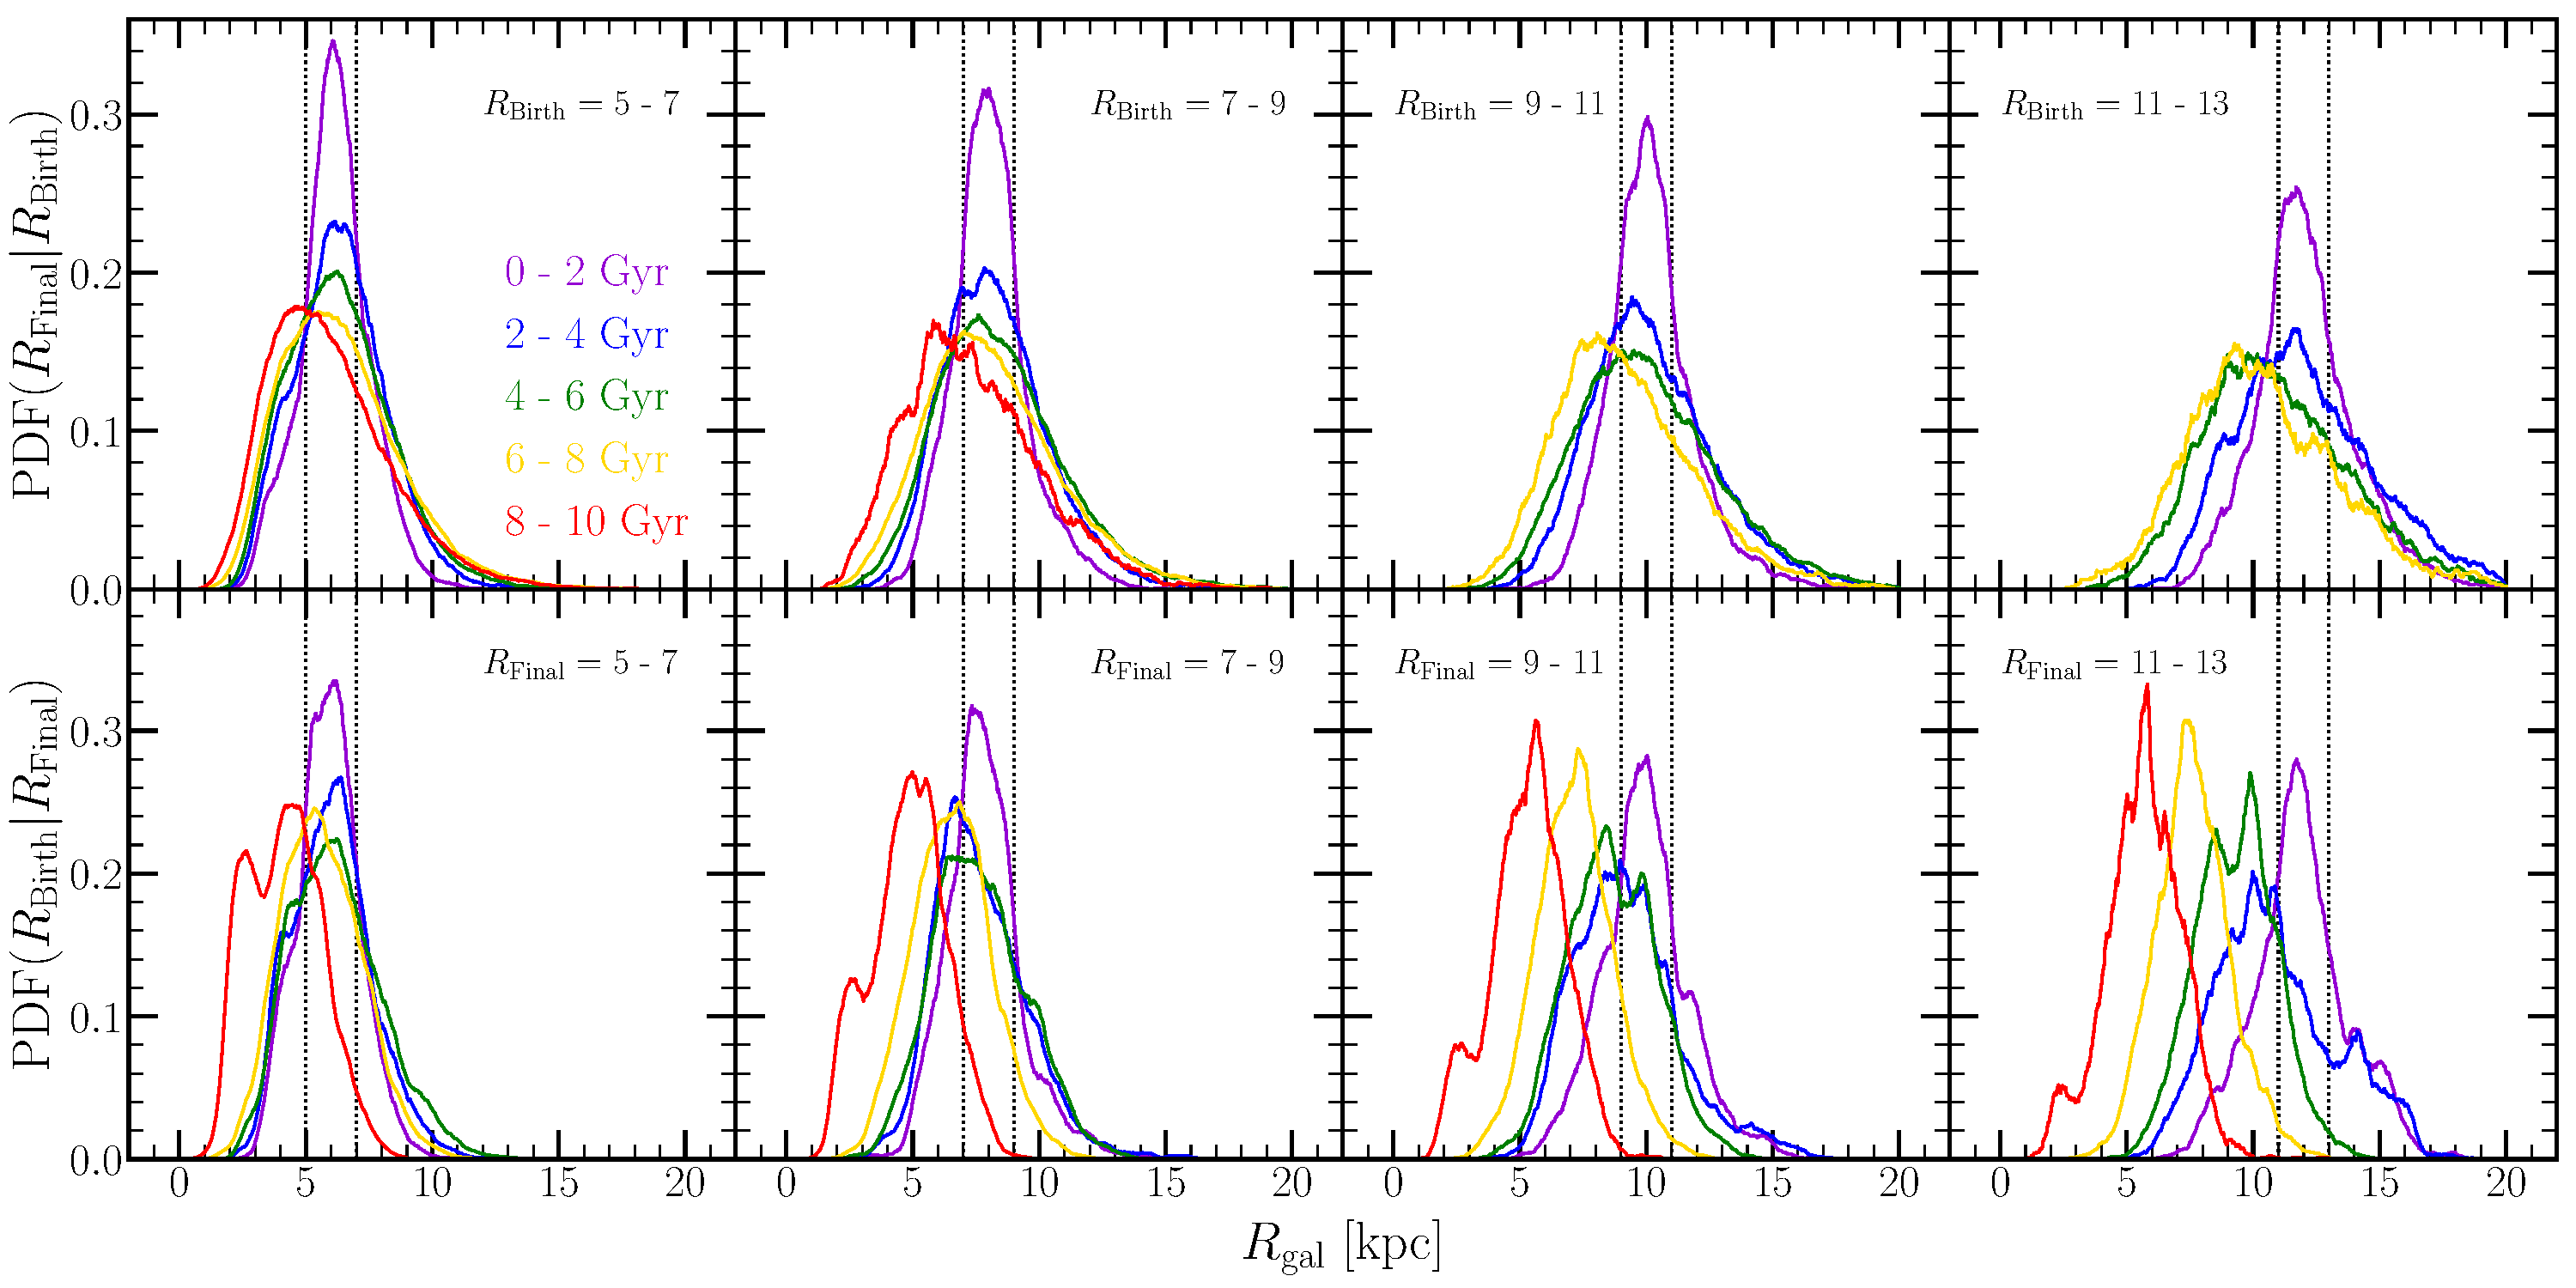
\includegraphics[scale = 0.38]{decomposition.pdf} 
\caption{Radial distributions of our sample of star particles from 
\texttt{h277}. In the top row, we show distributions of~\textit{final} radius 
in bins of birth radius and age, and in the bottom row, we show distributions 
of~\textit{birth} radius in bins of final radius and age. Each bin in 
Galactocentric radius is shown in its own panel, denoted in text at the top of 
each panel and by vertical black dashed lines. We colour-code the distributions 
according to the age of the star particles, denoted by the legend in the upper 
left panel. We smooth all distributions with a box-car width of 0.5 kpc to 
improve visual clarity. We omit the distributions for 8 - 10 Gyr old stars born 
in the 9 - 11 and 11 - 13 kpc bins due to an insufficient number of star 
particles with which to calculate the distribution. } 
\label{migration:fig:h277_decomposition} 
\end{figure*}
\end{landscape}
\clearpage
}

In the top row of Fig.~\ref{migration:fig:h277_decomposition}, we plot the distributions 
of final radius in bins of birth radius and age for our sample of star 
particles. 
Conversely, the bottom row shows distributions of birth radii in bins of final 
radius and age. 
Focusing on the top row of panels, we note that for star particles born at any 
radius and time, the distribution of final radius is still peaked near the 
birth radius, but the peak moves slightly inward with increasing age. 
The tails of the distributions toward larger~$\rgal$ are nearly 
age-independent, while the tails toward smaller~$\rgal$ are not. 
This suggests that radial migration inward and outward occur on different 
timescales in~\texttt{h277}, specifically that inward migration is slower than 
outward migration. 
By extension, this suggests that the two may be tied to different physical 
processes. 
Alternatively, it may simply be that stars that migrate to the outer Galaxy are 
no longer subject to strong dynamical perturbations while stars that move 
inward can still experience strong orbital disturbances. 
\par 
Focusing on the bottom row of panels in Fig.~\ref{migration:fig:h277_decomposition}, we 
note that the modes of the birth radius distributions show a much stronger 
dependence on age than the modes of the final radius distributions. 
At any Galactocentric radius at the present day, the youngest stars are 
overwhelmingly born at comparable radii, while the oldest stars are 
overwhelmingly born at smaller radii. 
This trend is most noticeable at large~$\rgal$. 
The differences between the final radius and birth radius distributions can be 
understood by considering the radial gradient of stellar surface density: there 
are more stars at small radius to move outward than vice versa, so roughly 
symmetric evolution of~$R_\text{final}$ produces strongly asymmetric evolution 
of~$R_\text{birth}$. 
\par 
Taking~$\left|\Delta \rgal\right| \geq$~500 pc 
between birth and final radii as the criterion for migration inward or outward, 
we find as global percentages in our sample that 27\% of star particles 
migrated inward, 29\% migrated outward, and the remaining 44\% stayed near 
their birth radius. 
As one can see from the top panels of Fig.~\ref{migration:fig:h277_decomposition}, a 
large fraction of migration away from birth radius has already occurred by the 
time stars are~$\sim$2 Gyr old. 
If the SN Ia delay-time distribution (DTD) is a~$t^{-1.1} \approx t^{-1}$ 
power-law as suggested by observational results~\citep[e.g.][]{Maoz2012a, 
Maoz2017}, then we expect similar numbers of SN Ia events to occur with delay 
times between 0.1 - 1 Gyr and 1 - 10 Gyr. 
With an extended DTD and the timescales for migration implied by 
Fig.~\ref{migration:fig:h277_decomposition}, SN Ia progenitors can migrate significant 
distances before exploding. 
This effect has largely been neglected by GCE studies to date on the grounds 
that radial migration is a slow process, and thus the majority of 
nucleosynthesis should occur near a star's birth radius (e.g. as assumed in 
\citealp{Minchev2013}, and the application of the~\citealp*{Weinberg2017b} 
analytic models in~\citealp{Feuillet2018}). 
However, we show below that radial migration within the timescale of the SN Ia 
DTD can have an important impact on some aspects of chemical evolution. 

% \begin{table} 
% % \color{red} 
% \caption{
% For a given quantity in the model, this table summarizes whether it is 
% adopted from~\hsim~or if it is specified as a model parameter. 
% } 
% \begin{tabularx}{\columnwidth}{l @{\extracolsep{\fill}} r} 
% % \resizebox{\columnwidth}{!}{ 
% % \begin{tabular}{l r} 
% \hline 
% \hline 
% Quantity & Source 
% \\ 
% \hline 
% Birth orbital radius of a stellar population & Model 
% \\ 
% Change in orbital radius of a stellar population & \hsim 
% \\ 
% Time-dependence of the change in orbital radius & Model 
% \\ 
% Present-day midplane distance of a stellar population (\absz) & \hsim 
% \\ 
% Star Formation History & Model 
% \\ 
% Nucleosynthetic Yields & Model 
% \\ 
% Outflows from the ISM & Model 
% \\ 
% Star Formation Law & Model 
% \\ 
% Surface Density Gradient & Model 
% \\ 
% \hline 
% \end{tabularx} 
% % } 
% % \label{migration:tab:params} 
% \label{migration:tab:which} 
% \end{table} 

\subsection{Radial Migration} 
\label{migration:sec:methods:migration} 
As in previous studies~\citep[e.g.][]{Matteucci1989, Schoenrich2009a, 
Minchev2013, Sharma2021}, in this paper we model the Milky Way as a series of 
concentric rings\footnote{
	For clarity, we use the term ``ring'' to refer to a computational zone of 
	our calculation (100 pc in radial range) and the term ``annulus'' to refer 
	to a larger radial range (typically 2 kpc). 
} with a uniform width~$\delta \rgal$. 
To run numerical simulations of these models, we develop and make use 
of~\vice's~\texttt{milkyway} object, designed specifically for such an 
approach. 
The~\texttt{milkyway} object is a subclass of a more general object named 
\texttt{multizone}; at its core a~\texttt{multizone} object is an array of 
\texttt{singlezone} objects, which are designed to handle one-zone models of 
GCE and were the focus of~\citet{Johnson2020},~\vice's initial release paper. 
The~\texttt{multizone} object affords users full control over which zone any 
individual stellar population is in at all timesteps following its formation as 
well as the ability to move gas between any two zones with any time dependence. 
In principle this should allow for arbitrarily complex zone configurations and 
migration prescriptions. 
The~\texttt{milkyway} object is a user-friendly extension of the 
\texttt{multizone} base class, which enforces an annular zone configuration as 
we take here. 
As defaults, it adopts the stellar migration model detailed in this section, 
our star formation law discussed in~\S~\ref{migration:sec:methods:sfe}, and the scaling 
of the outflow mass loading factor~$\eta$ with radius~\rgal~parameterized 
in~\S~\ref{migration:sec:methods:outflows}. 
\par 
As in hydrodynamical simulations, star particles in~\vice~are stand-ins for 
entire stellar populations. 
They are said to be in a given zone if their radius is between the inner and 
outer edges of the ring. 
At all times, their nucleosynthetic products and returned envelopes are placed 
in the ISM of the ring that they are in~\textit{at that time}. 
\vice~forms a fixed number of stellar populations per zone per timestep, and it 
allows their masses to vary to account for variations in the SFR. 
The total mass of stars formed in a given zone and timestep is divided evenly 
among the corresponding stellar populations, which can then experience 
different stellar migration histories. 
\par 
The final radius of a stellar population is then determined based on the birth 
and final radii of star particles in the hydrodynamical simulation. 
Describing the Galaxy as a series of concentric rings,~\vice's~
\texttt{milkyway} object assumes stellar populations are born at the centres of 
each ring. 
For a stellar population born at a time~$T$ and Galactocentric radius 
$\rgal$, it first searches for star particles from~\texttt{h277} that 
formed at~$T \pm$~250 Myr and~$\rgal \pm$~250 pc. 
It then randomly selects a star particle from this subsample to act as an 
\textit{analogue}. 
This stellar population then adopts the %{\color{red} 
present day midplane 
distance~$z$ and the
%} 
change in orbital radius 
$\Delta \rgal$ of its analogue, and moves from its birth radius to the 
implied final radius and~$z$ at~$T$ = 13.2 Gyr with an assumed time dependence 
(see below). 
If no candidate analogues are found,~\vice~widens the search to~$T \pm$~500 Myr 
and~$\rgal \pm$~500 pc. 
If still no analogue is found, then it finds the star particle with the 
smallest difference in birth radius still within a birth time of $T \pm$~500 
Myr, and assigns it as the analogue. 
% {\color{red} 
Because we remove bulge, pseudobulge, and halo star particles from our sample 
(see discussion in~\S~\ref{migration:sec:methods:h277}), every assigned analogue is a 
star particle with disc-like kinematics. 
Since~\hsim~has a similar final disc scale length as the Milky 
Way~\citep{Bird2021}, we do not normalize radii by this quantity prior to 
conducting the analogue search. 
When an~\hsim~star particle is assigned as an analogue, it is~\textit{not} 
thrown out of the sample of candidate analogues, in theory allowing a star 
particle to act as an analogue for multiple stellar populations. Because these 
populations will have similar~$R_\text{form}$~and~$T_\text{form}$, they will 
have similar but not identical abundances. 
% }
\par 
While this prescription allows stellar populations to be assigned analogues 
with significantly different birth radii, this is only an issue for small~$T$ 
and large~$\rgal$ where %{\color{red} 
only a small fraction of~\hsim's star 
particles reside,
% } 
% there are few star particles from~\hsim, 
and where few stars form in nature anyway due to the inside-out growth of 
galaxies~\citep[e.g.][]{Bird2013}. 
% {\color{red} 
In practice, we find that our sample of star particles is sufficiently large 
such that our model is still able to assign the vast majority of stellar 
populations born at large~\rgal~($\gtrsim$10 kpc) and small~$T$ 
(age~$\gtrsim$10 Gyr) an analogue which formed within~$\sim$2 kpc of its birth 
radius. 
Although the models we present in this paper do impose a small but non-zero 
level of star formation at early times and large radii (see Fig.~\ref{migration:fig:evol} 
and the associated discussion in~\S~\ref{migration:sec:methods:sfhs}), this ensures that 
those stellar populations inherit plausible dynamics from the~\hsim~star 
particles. 
% }
Furthermore, due to the similarity of the histograms in the top row of 
Fig.~\ref{migration:fig:h277_decomposition}, we expect taking~$\Delta \rgal$ from 
a star particle that formed at a similar time but different birth radius in 
these instances to be accurate enough for our purposes. 
% {\color{red}
In exploratory work for this paper, we also considered a migration model in 
which stellar populations remain at their birth radius if no analogue born 
within~$\rgal~\pm$~500 pc and~$T~\pm$~500 Myr is found. 
We find similar results in this case, suggesting that our qualitative 
conclusions are largely unaffected by the fine details of the dynamical 
history. 
% }
% When an~\hsim~star particle is assigned as an analogue, it is~\textit{not} 
% thrown out of the sample of candidate analogues, in theory allowing a star 
% particle to act as an analogue for multiple stellar populations. Because these 
% populations will have similar~$R_\text{form}$~and~$T_\text{form}$, they will 
% have similar but not identical abundances. 

% fig 2 
\begin{figure} 
\centering 
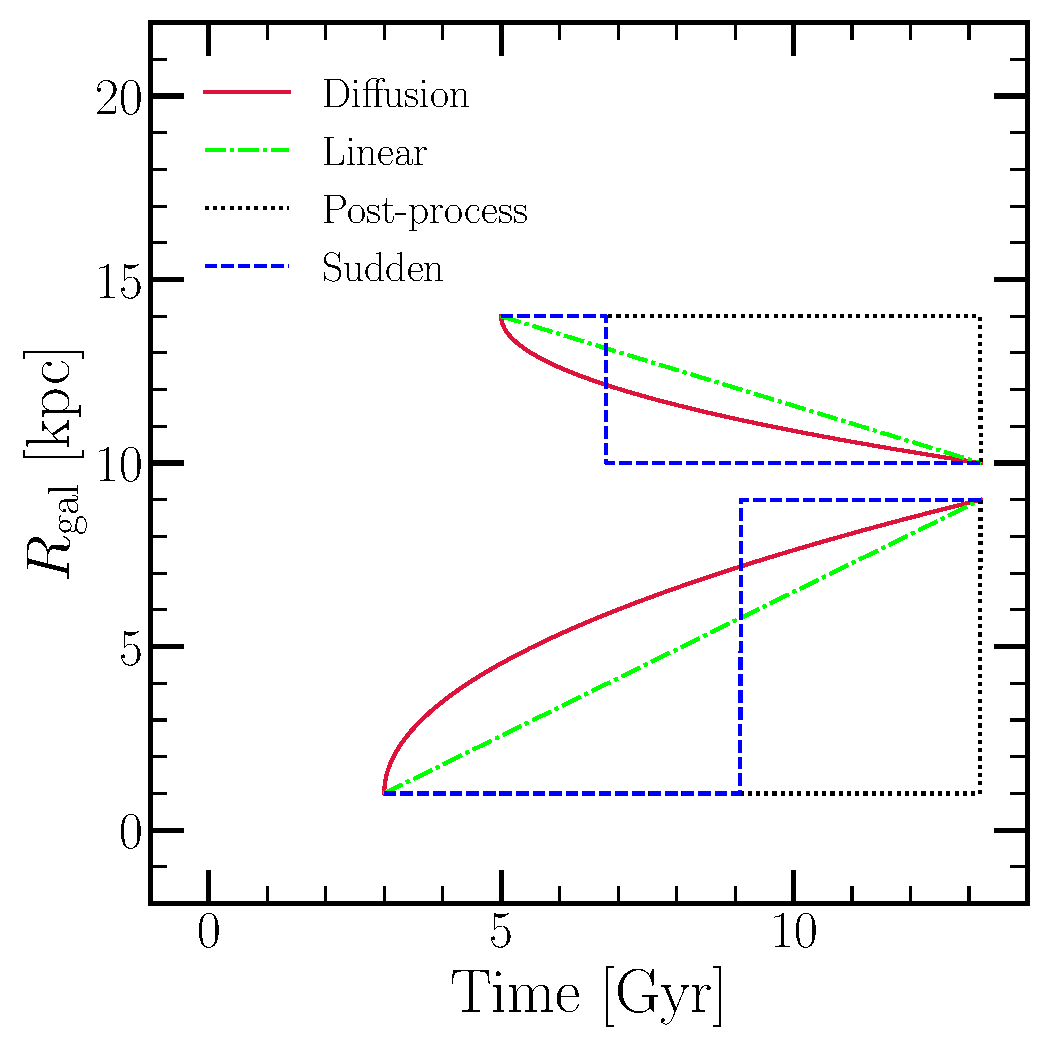
\includegraphics[scale = 0.7]{migration.pdf} 
\caption{
A diagram illustrating how Galactocentric radius changes with time for 
two stellar populations under our migration schema: diffusion (crimson, solid), 
linear (lime, dot-dashed), post-process (black, dotted), and sudden (blue, 
dashed). Here the initial and final radii and birth times are chosen at random 
for illustrative purposes. With the initial and final Galactocentric radii of 
a stellar population, its birth time, and one of these assumptions regarding 
the time-dependence of radial migration, the Galactocentric radius at all times 
is known. Diffusion is our default model.
} 
\label{migration:fig:migration_schema} 
\end{figure} 

We neglect radial gas flows in the present paper~\citep{Bilitewski2012, 
Lacey1985}, instead focusing our comparisons on the time-dependence with which 
stars migrate. 
We consider four models describing the evolution between a star particle's 
birth and final radius: 
\begin{itemize} 
	\item \textbf{Post-Processing}: Stars stay where they are born until the 
	final timestep, at which point they instantly migrate to their final 
	radius. 
	This retains the assumption that stars do not contribute to nucleosynthesis 
	beyond their birth radius as employed in previous studies 
	\citep[e.g.][]{Minchev2013}. 
	In this scenario, the ISM of each ring is treated as a one-zone model 
	independent of all other zones. We illustrate this case with a black dotted 
	line in Fig.~\ref{migration:fig:migration_schema}. 

	\item \textbf{Sudden}: A random number is drawn from a uniform distribution 
	between a stellar population's time of birth and the present day. 
	That time is taken to be the time of instantaneous migration to the 
	present-day annulus. 
	This emulates a scenario in which a single dynamical interaction rapidly 
	changes a star's orbital radius, and it can be thought of mathematically as 
	a generalization of the post-processing scenario. 
	We illustrate this case with a blue dashed line in 
	Fig.~\ref{migration:fig:migration_schema}. 

	\item \textbf{Diffusion}: Stars move to their final radii in a continuous, 
	time-dependent manner, with displacement~$\propto \sqrt{\text{age}}$. 
	This scenario corresponds to diffusion of angular momentum by a random 
	walk, similar to the assumption used by~\citet{Frankel2018, Frankel2020}. 
	We illustrate this case with a red solid line in 
	Fig.~\ref{migration:fig:migration_schema}. 

	\item \textbf{Linear}: A simple variation of the diffusion model in which 
	the migration to the final radius scales linearly with age rather than with 
	$\sqrt{\text{age}}$. We illustrate this case with a green dot-dashed line 
	in Fig.~\ref{migration:fig:migration_schema}. 
\end{itemize} 
The diffusion model has the clearest physical motivation, and it is our default 
assumption used in all cases unless otherwise noted. 
The other models provide illustrative contrasts and allow us to investigate our 
model's sensitivity to the details of radial migration. 
We do not distinguish between ``blurring'' and ``churning'' 
\citep{Schoenrich2009a}, terms frequenly used to refer to a star's epicyclic 
motions and changes in the guiding centre of its orbit, respectively. 
% We do not distinguish between ``blurring'' and ``churning'', terms frequently 
% used to refer to a star's epicyclic motions and changes in the guiding centre 
% of its orbit~\citep[e.g.][]{Sellwood2002, Schoenrich2009a}. 
Both effects, induced by a wide variety of underlying causes such as molecular 
cloud scattering~\citep{Mihalas1981, Jenkins1990, Jenkins1992}, orbital 
resonances with spiral arms or bars~\citep{Sellwood2002, Minchev2011}, and 
satellite perturbations~\citep{Bird2012}, are present in the~\hsim~simulation. 
\par 
Our GCE model assumes that the star-forming ISM is vertically and azimuthally 
mixed within each radial annulus. 
The abundances assigned to a stellar population depend on its birth radius and 
time, but they do not depend on its distance from the plane. 
Nonetheless, as shown below, the abundance patterns of our simulation exhibit 
clear vertical gradients because older stellar populations have thicker 
vertical distributions~\citep{Bird2021}. 
Radial migration is also coupled to vertical dynamics in complex ways 
\citep{Solway2012, Minchev2012}. 
We will see that these effects already suffice to explain many of the observed 
vertical trends of Milky Way disc abundances. 


% \subsection{Nucleosynthetic Yields, Outflows, and Recycling} 
% \label{migration:sec:methods:yields} 
\subsection{Nucleosynthetic Yields} 
\label{migration:sec:methods:yields} 
We focus our analysis on alpha and iron-peak elements, taking oxygen (O) and 
iron (Fe) as the representative cases. 
The dominant enrichment channels of interest in our models are thus CCSN and 
SN Ia~\citep{Johnson2019}. 
We would expect similar results for other alpha (e.g. Ne, Mg, Si) and 
iron-peak elements (e.g., Cr, Ni), with quantitative differences reflective of 
their relative yields. 
Odd-$Z$ iron-peak elements (e.g., V, Mn, Co) could behave somewhat distinctly 
because of metallicity-dependent yields. 
\par 
CCSN enrichment happens immediately following the formation of progenitor stars 
in~\vice. 
This is an adequate approximation, because the lifetimes of massive stars are 
short compared to the relevant timescales for galaxy evolution. 
For the most massive stars, the lifetimes are comparable to the timestep size 
we adopt in our numerical integrations. 
This assumption implies a linear relationship between the CCSN enrichment 
rate and the SFR: 
\begin{equation} 
\dot{M}_x^\text{CC} = y_x^\text{CC}\dot{M}_\star 
\end{equation} 
where~$y_x^\text{CC}$ is the CCSN yield of some element~$x$. Physically, this 
quantity represents the mass of an element~$x$ ejected to the ISM from all 
CCSN events associated with a stellar population in units of the stellar 
population's initial mass. 
For example, if~$y_x^\text{CC} = 0.01$, a hypothetical 100~\msun~stellar 
population would add 1~\msun~of~$x$ to the ISM immediately. 
In this paper, we adopt~$y_\text{O}^\text{CC}$ = 0.015 and 
$y_\text{Fe}^\text{CC}$~= 0.0012 from~\citet{Johnson2020}, who in turn adopt 
these values from~\citet{Weinberg2017b}. 
\par 
SN Ia nucleosynthesis products are injected according to a~$t^{-1.1}$ DTD with 
a minimum delay time of~$t_\text{D}$ = 150 Myr. 
This is the default DTD in~\vice, which was also adopted by 
\citet{Johnson2020}, and is suggested by recent observational results comparing 
the cosmic SN Ia rate to the cosmic SFH~\citep{Maoz2012a, Maoz2017}. 
In a one-zone model at times~$t > t_\text{D}$, the enrichment rate of some 
element~$x$~can be expressed as the product of some yield~$y_x^\text{Ia}$ and 
the SFH weighted by the DTD: 
\begin{subequations}\begin{align} 
\dot{M}_x^\text{Ia} &= y_x^\text{Ia}\langle\dot{M}_\star\rangle_\text{Ia} \\ 
&= y_x^\text{Ia}\ddfrac{
	\int_0^t \dot{M}_\star(t') R_\text{Ia}(t - t') dt' 
}{
	\int_{t_\text{D}}^{t_\text{max}} R_\text{Ia}(t')dt' 
} 
\label{migration:eq:mdot_ia} 
\end{align}\end{subequations} 
where~$R_\text{Ia}$ is the DTD itself, which has units of~$M_\odot^{-1}$ 
Gyr$^{-1}$. 
Like the CCSN yield,~$y_x^\text{Ia}$ is the mass of some element~$x$ produced 
by SNe Ia over the time interval~$t_\text{D} - t_\text{max}$, in units of the 
stellar population's initial mass. 
It can also be expressed as an integral over the DTD: 
\begin{equation} 
y_x^\text{Ia} = m_x^\text{Ia} \int_{t_\text{D}}^{t_\text{max}} R_\text{Ia}(t') 
dt' = m_x^\text{Ia}\frac{N_\text{Ia}}{M_\star} 
\label{migration:eq:y_x_ia} 
\end{equation} 
where~$m_x^\text{Ia}$ is the average mass of the element~$x$ produced in a 
single SN Ia event and the integral evaluates to the mean number of SN Ia 
events~$N_\text{Ia}$ per mass of stars formed~$M_\star$. 
\vice~forces~$t_\text{max}$~= 15 Gyr always, though provided one is consistent 
with equations~\refp{migration:eq:mdot_ia} and~\refp{migration:eq:y_x_ia}, the results are 
independent of~$t_\text{max}$ because the integrals cancel. 
Extending this formalism to multi-zone models is simple; rather than an 
integral over the star formation history of a given annulus, the rate becomes 
a summation over all stellar populations that are in a given zone at some time: 
\begin{equation} 
\dot{M}_x^\text{Ia} = y_x^\text{Ia} \ddfrac{
	\sum_i M_i R_\text{Ia}(\tau_i) 
}{
	\int_{t_\text{D}}^{t_\text{max}} R_\text{Ia}(t')dt' 
} 
\label{migration:eq:mdot_ia_multizone} 
\end{equation} 
where~$M_i$~and~$\tau_i$~are the mass and age of the~$i$'th stellar population, 
respectively. 
\par 
Initially, we adopted~$y_\text{O}^\text{Ia}$~= 0 and~$y_\text{Fe}^\text{Ia}$~= 
0.0017 from~\citet{Johnson2020}, who in turn adopt these values from 
\citet{Weinberg2017b}. 
However, we found that the e-folding timescales of star formation in our models 
are sufficiently long (see discussion in~\S~\ref{migration:sec:methods:sfhs}) that our 
fiducial, inside-out SFH model predicted [O/Fe]~$\approx$~+0.05 for young 
stars. 
We therefore multiply~$y_\text{Fe}^\text{Ia}$~by~$10^{0.1}$, adopting 
$y_\text{Fe}^\text{Ia}$~= 0.00214 so that our fiducial model predicts a 
late-time [O/Fe] ratio in better agreement with observations. 
Changes at this level are within the uncertainties of SN Ia rates and yields, 
so we consider it reasonable to adjust the yields empirically to reproduce 
observed abundances. 
\par 
Our IMF-averaged O and Fe yields are based on a~\citet{Kroupa2001} IMF combined 
with supernova nucleosynthesis models in which most~$M > 8~\msun$ stars explode 
as a CCSN~\citep[e.g.][]{Chieffi2004, Chieffi2013}. 
Recent studies have strongly suggested that many high mass stars instead 
collapse directly to a black hole (see theoretical discussion by, e.g., 
\citealp{Pejcha2015, Sukhbold2016, Ertl2016}, and observational evidence from 
\citealp*{Gerke2015};~\citealp{Adams2017, Basinger2021}). 
Our yields would be lower in a scenario with extensive black hole formation 
and/or a steeper high mass IMF~\citep{Griffith2021b}. 
These effects could also introduce a metallicity dependence if the landscape of 
black hole formation changes with metallicity. 
The strong increase of the specific SN Ia rate seen at low galaxy masses 
\citep{Brown2019} provides circumstantial evidence of a higher~$R_\text{Ia}$ 
normalization at low metallicity; the stellar close binary fraction also 
depends on metallicity (\citealp{Badenes2018};~\citealp*{Moe2019}). 
However, there is presently no solid empirical basis for adopting metallicity 
dependent O and Fe yields over the range relevant to this paper (roughly 
-0.8~$\leq$~\feh~$\leq$~0.4), and some empirical evidence that any metallicity 
trends in this range are weak~\citep{Weinberg2019}. 
\vice~has capabilities to compute IMF-averaged yields for a flexible 
description of the massive star explodability landscape, as described 
by~\citet{Griffith2021b} and the~\vice~documentation, but we do not use this 
methodology here. 
We expect that most of our results would be largely unchanged if we were to 
lower all three yields ($y_\text{O}^\text{CC}$, $y_\text{Fe}^\text{CC}$, 
$y_\text{Fe}^\text{Ia}$) by the same factor and adjust our adopted outflow 
mass loading prescription to compensate (see below). 
\par 
Both AGB star enrichment and the recycling of previously produced metals in 
this paper proceed as they did in~\citet{Johnson2020}, with the caveat that the 
mass is added to the ring that a stellar population is in at a given time, 
which may or may not be the ring it was born in. 
Recycling proceeds according to the~\citet{Kalirai2008} initial-remnant mass 
relation assuming a~\citet{Kroupa2001} IMF and a mass-lifetime relationship of 
$\tau = 1.1\tau_\odot(M/M_\odot)^{-3.5}$, where~$\tau_\odot$~= 10 Gyr is the 
main sequence lifetime of the sun and the factor of 1.1 accounts for the 
post-main sequence lifetime. 
\vice~includes AGB enrichment in all models; here we adopt the net yields 
sampled on a table of stellar initial mass and metallicity from the FRUITY 
database~\citep{Cristallo2011, Cristallo2015}. 
However, the AGB star yields of O and Fe are tiny compared to their 
supernova yields, so they have negligible impact on the results presented in 
this paper. 

\subsection{Outflows} 
\label{migration:sec:methods:outflows} 
\citet{Weinberg2017b} demonstrate that, to first order, the nucleosynthetic 
yields of a given element and the strength of outflowing winds determine the 
late-time equilibrium abundance in the ISM, with a secondary dependence on the 
SFH. 
We retain their characterization of outflows here, in terms of a mass-loading 
factor~$\eta$~describing the ratio of the mass outflow to the SFR: 
\begin{equation} 
\eta \equiv \frac{\dot{M}_\text{out}}{\dot{M}_\star}. 
\end{equation} 
We adopt a scaling of~$\eta$~with~$\rgal$~such that the late-time 
equilibrium abundance as a function of radius describes a metallicity 
gradient in agreement with observations. 
For a constant SFR, the equilibrium abundance of an~$\alpha$-element, produced 
by CCSNe with a metallicity-independent yield, is given by 
\begin{equation} 
Z_{\alpha,\text{eq}} = \frac{y_\alpha^\text{CC}}{1 + \eta(\rgal) - r}, 
\end{equation} 
where~$r$~is the recycling parameter ($\approx$0.4 for the sake of this scaling 
with a~\citealp{Kroupa2001} IMF; see discussion in~\S~2.2 
of \citealp{Weinberg2017b}). Solving for~$\eta(\rgal)$ yields 
\begin{equation} 
\eta(\rgal) = \frac{y_\alpha^\text{CC}}{Z_{\alpha,\text{eq}}} + r - 1 = 
\frac{y_\alpha^\text{CC}}{Z_{\alpha,\odot}}10^{-\text{mode([$\alpha$/H])}
(\rgal)} + r - 1, 
\end{equation} 
where mode([$\alpha$/H])($\rgal$) denotes the mode of the stellar 
[$\alpha$/H] distribution at a radius~$\rgal$, which we assume to correspond 
to the equilibrium abundance at that radius. 
Recent studies of the disc metallicity gradient with APOGEE find values of 
-0.09 dex/kpc to -0.06 dex/kpc~\citep[e.g.][]{Frinchaboy2013, Hayden2014, 
Weinberg2019}, consistent with earlier studies. 
Here we adopt a slope of -0.08 dex/kpc and set mode([$\alpha$/H]) to be 
$\sim$+0.3 at~$\rgal$ = 4 kpc, producing mode([$\alpha$/H])~$\approx$ 0 at 
$\rgal$ = 7 - 9 kpc. This results in the following form for~$\eta$ as a 
function of Galactocentric radius: 
\begin{equation} 
\eta(\rgal) = \frac{y_\alpha^\text{CC}}{Z_{\alpha,\odot}} 
10^{(0.08\text{ kpc}^{-1})(\rgal - 4\text{ kpc}) - 0.3} + r - 1, 
\label{migration:eq:eta_rgal} 
\end{equation} 
where we adopt our CCSN yield of O for~$y_\alpha^\text{CC}$ and the solar 
photospheric abundance of O of~$Z_{\text{O},\odot}$ = 0.00572 based on 
\citet{Asplund2009}. 
We plot this adopted scaling in the top panel of Fig.~\ref{migration:fig:eta_tau_sfh}, 
highlighting a value of~$\sim$2.15 for the solar circle with a red dotted line. 
In Fig.~\ref{migration:fig:metallicity_gradient} below, we show that our full model 
including a time-dependent SFH and radial migration produces stellar and gas 
phase gradients similar but not identical to those of equation 
\refp{migration:eq:eta_rgal}. 
In Figs.~\ref{migration:fig:mdf_3panel_fe} and~\ref{migration:fig:mdf_3panel_o} below, we show that 
the model achieves qualitative agreement with the metallicity gradient observed 
by APOGEE. 

% fig 3 
\begin{figure} 
\centering 
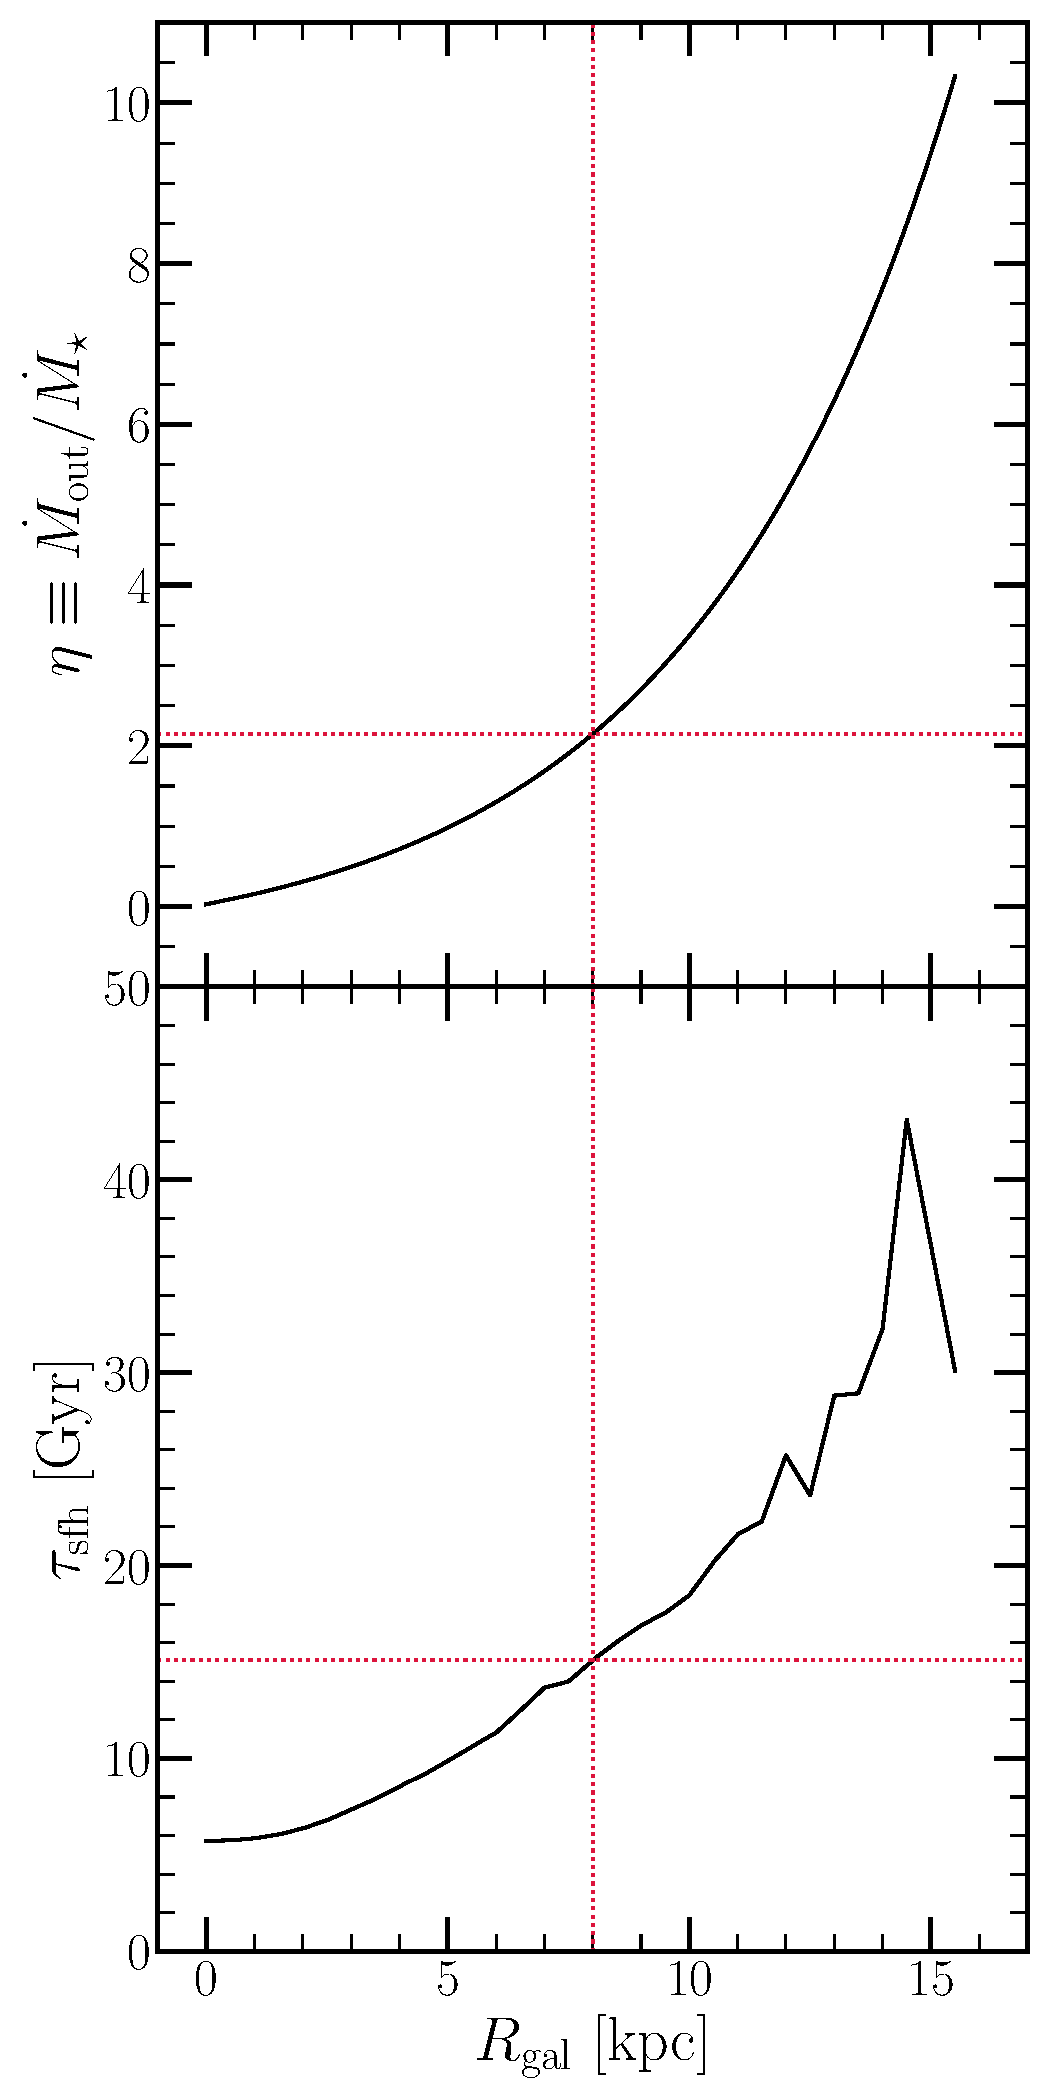
\includegraphics[scale = 0.45]{eta_tau_sfh.pdf} 
\caption{\textbf{Top}: Our implemented scaling of the mass loading factor 
$\eta$~with Galactocentric radius (black) as defined by equation 
\refp{migration:eq:eta_rgal}.~\textbf{Bottom}: The e-folding timescales of the star 
formation histories of our model galaxies (black). These values come from a 
fit to the~$\Sigma_\star$-age relation in bins of~$R/R_\text{e}$~for 
$10^{10.5}$~-~$10^{11}$~\msun~Sa/Sb Hubble type spiral galaxies as reported by 
\citet[][see discussion in~\S~\ref{migration:sec:methods:sfhs}]{Sanchez2020}. The 
horizontal and vertical red dashed lines in both panels highlight a mass 
loading factor of~$\eta \approx$~2.15 and a star formation timescale of 
$\tau_\text{sfh} \approx$~15 Gyr at an assumed radius of the sun of 
$R_\odot$ = 8 kpc. } 
\label{migration:fig:eta_tau_sfh} 
\end{figure} 

\subsection{Star Formation Histories} 
\label{migration:sec:methods:sfhs} 
\vice~computes models in either ``infall'', ``star formation'', or ``gas'' 
mode, referring to which component of the evolutionary history the user has 
specified. 
The starburst models of~\citet{Johnson2020} ran in infall mode, 
meaning that the gas infall rate is specified and the SFR follows from the gas 
surface density and adopted star formation law. 
Here we run~\vice~in star formation mode so that we achieve a specified form of 
the SFHs in our models. 
In Appendix~\ref{migration:sec:normalize_sfh}, we explain how we normalize the parameters 
of our SFHs to produce a realistic model Galaxy at the present day. 
In short, we take a unitless description of the time-dependence of the SFH at a 
given Galactocentric radius, denoted~$f(t|\rgal)$, and a unitless description 
of the present day stellar surface density gradient, denoted~$g(\rgal)$. 
We integrate~$f(t|\rgal)$ with time for each annulus, assuming~$\rgal$ to 
correspond to the centre of the zone, and attach a prefactor to 
$f(t|\rgal)$ in each annulus such that the desired gradient is achieved 
with a total stellar mass similar to the Milky Way. 
This procedure neglects the impact of radial migration, assuming that it does 
not significantly alter the form of~$g(\rgal)$. 
% {\color{red} 
We find this to be true for our sample of~\hsim~star particles, and we 
demonstrate that this assumption holds in our chemical evolution models 
in~\S~\ref{migration:sec:methods:surface_density_gradient}, where we also detail our 
adopted form of~$g(\rgal)$. 
% }
% We demonstrate that this assumption holds 
% in~\S~\ref{migration:sec:methods:surface_density_gradient}, in which we also detail our 
% adopted form of~$g(\rgal)$. 
The equation derived in Appendix~\ref{migration:sec:normalize_sfh} can be used to 
calculate these prefactors for alternative models of Milky Way-like galaxies. 
\par 
In the present paper, we consider four forms of the SFH, which we dub 
``constant'', ``inside-out'', ``late-burst'', and ``outer-burst''. 
They are defined as follows: 
\begin{itemize} 
	\item \textbf{Constant}: The SFH at a given radius is time-independent, 
	\begin{equation} 
	f_\text{C}(t|\rgal) = 1. 
	\label{migration:eq:constant_sfh} 
	\end{equation} 
	This case is of theoretical interest because it quantifies the effect of 
	stellar migration while removing the impact of a time-dependent SFH. 

	\item \textbf{Inside-Out}: This is our fiducial SFH, 
	\begin{equation} 
	f_\text{IO}(t|\rgal) = (1 - e^{-t / \tau_\text{rise}}) 
	e^{-t / \tau_\text{sfh}}. 
	\label{migration:eq:insideout_sfh} 
	\end{equation} 
	We adopt this mathematical form over the somewhat more common 
	$te^{-t/\tau_\text{sfh}}$ because it allows separate control over the 
	rising and falling phase of the SFH. 
	Equation~\refp{migration:eq:insideout_sfh} has a maximum near~$\tau_\text{rise}$, 
	which in this paper we set to 2 Gyr at all radii. 
	This form produces a peak in star formation at lookback times of~$\sim$11 
	Gyr, roughly corresponding to a redsfhit of~$z \approx$ 2.5. 
	% {\color{red} 
	In detail, however, the time of peak star formation increases 
	with~$\tau_\text{sfh}$, which in turn increases with~\rgal~in our models 
	(see discussion below). 
	As a result,~$\dot{\Sigma}_\star$ in the outer disc instead reaches its 
	peak at lookback times of~$\sim$7 - 8 Gyr, qualitatively consistent with 
	the radial growth of disc galaxies~\citep{Bird2013, Bird2021, Frankel2019}. 
	% } 
	% We discuss the choice of~$\tau_\text{sfh}$ below. 

	\item \textbf{Late-Burst}: In this model, the inside-out SFH is modified to 
	exhibit a recent, slow ``burst'' in star formation described by a Gaussian 
	in time: 
	\begin{equation} 
	f_\text{LB}(t|\rgal) = f_\text{IO}(t|\rgal) 
	\left(1 + A_be^{-(t - t_b)^2/2\sigma_b^2}\right), 
	\label{migration:eq:lateburst_sfh} 
	\end{equation} 
	where $A_b$ is a dimensionless parameter describing the strength of the 
	starburst,~$t_b$ is the time of the local maximum in the SFH during the 
	burst, and~$\sigma_b$ is the width of the Gaussian describing it. 
	To approximate the findings of~\citet{Mor2019} and~\citet{Isern2019}, we 
	adopt~$A_b$ = 1.5,~$t_b$ = 11.2 Gyr, and~$\sigma_b$ = 1 Gyr, finding 
	that~$A_b$ = 1.5 with a declining~$f_\text{IO}(t|\rgal)$ produces a local 
	maximum SFR that is a factor of~$\sim$2 larger than the preceding local 
	minimum. 

	\item \textbf{Outer-Burst}: A variation of the late-burst model in which 
	only zones at~$\rgal \geq$~6 kpc experience the starburst, with inner 
	regions following the inside-out SFH. 
	Because the empirical evidence for elevated recent star formation comes 
	from local observations, it is useful to investigate the case where it is 
	confined to the outer Galaxy. 
	In their hydrodynamical simulation of a Milky Way-like galaxy, 
	\citet{Vincenzo2020} find that satellite perturbations enhance gas 
	accretion preferentially in the outer regions. 
\end{itemize} 

% fig 4
\afterpage{
\clearpage
\begin{landscape}
\begin{figure*} 
\centering 
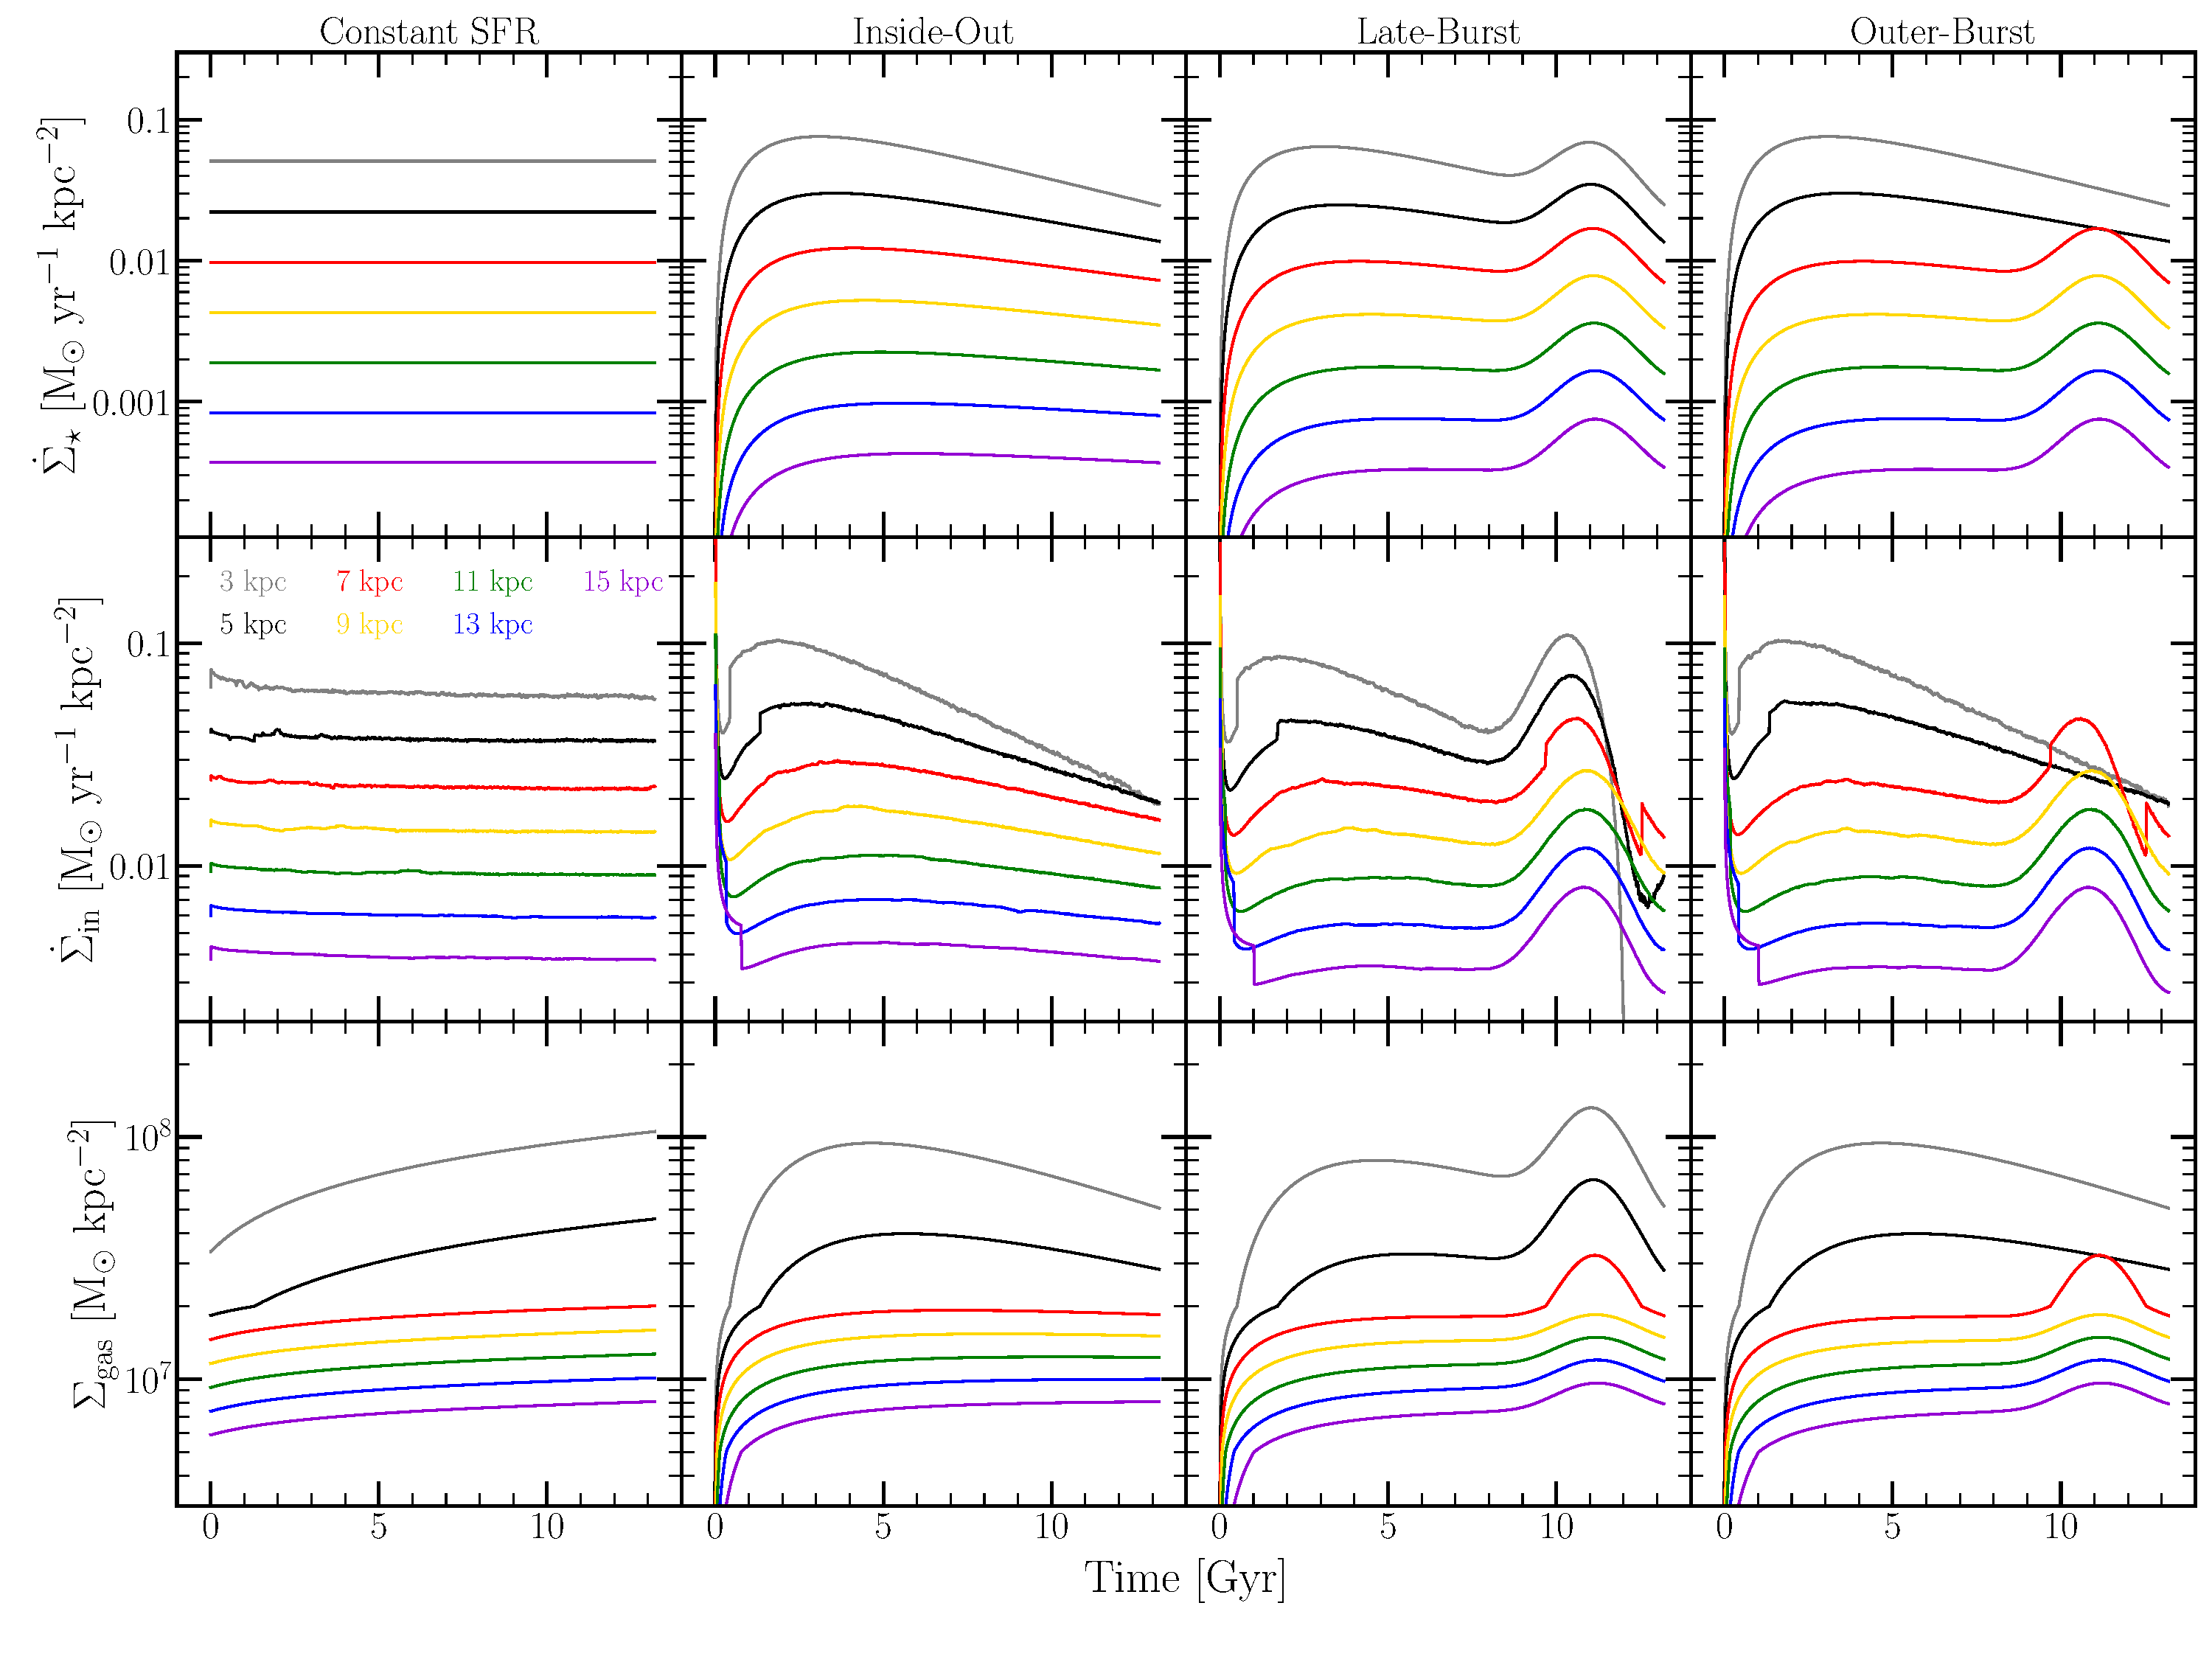
\includegraphics[scale = 0.34]{evol.pdf} 
\caption{The surface densities of star formation~$\dot{\Sigma}_\star$ (top 
row), infall $\dot{\Sigma}_\text{in}$ (middle row), and gas~$\Sigma_\text{g}$ 
(bottom row) as functions of simulation time for our four fiducial SFHs: 
constant (far left), inside-out (left middle), late-burst (right middle), and 
outer-burst (far right). We plot curves for the rings whose inner radii are 
3 kpc (grey), 5 kpc (black), 7 kpc (red), 9 kpc (yellow), 11 kpc (green), 13 
kpc (blue), and 15 kpc (purple) (see equations~\refp{migration:eq:constant_sfh}, 
\refp{migration:eq:insideout_sfh}, and~\refp{migration:eq:lateburst_sfh} for the mathematical 
definition of each SFH). 
}
\label{migration:fig:evol} 
\end{figure*}
\end{landscape}
\clearpage
}

The inside-out model is our fiducial choice, and it is the model shown in 
figures unless otherwise specified. 
The constant SFR model allows us to investigate the impact of migration when 
the time-dependence of the SFH is removed, and the two burst models allow us to 
explore the consequences of elevated recent star formation supported by some 
recent data. 
% {\color{red} 
More complex scenarios, such as multiple bursts induced by repeated satellite 
passages~\citep[e.g.][]{Lian2020a, Lian2020b, RuizLara2020, Sysoliatina2021} or 
the onset of star formation occurring later in the outer disc to better capture 
the radial growth of the Galaxy~\citep[e.g.][]{Frankel2019}, can be 
explored easily using~\vice, but we do not explore such models here. 
% } 
% More complex scenarios with multiple bursts induced by repeated satellite 
% passages~\citep[e.g.][]{Lian2020a, Lian2020b, RuizLara2020, Sysoliatina2021} 
% can be modeled easily in~\vice, but we do not explore them here. 
\par 
We derive the~$\tau_\text{sfh}-\rgal$ relation from the data of 
\citet{Sanchez2020}, who presents the stellar surface density~$\Sigma_\star$ as 
a function of age in bins of~$R/R_\text{e}$ for MaNGA 
galaxies~\citep{Bundy2015}, where $R_\text{e}$ is the half-light radius. 
Here we take the~$M_\star = 10^{10.5} - 10^{11}~\msun$~bin for Sa/Sb spirals 
and simultaneously fit the normalization and e-folding timescale 
$\tau_\text{sfh}$ of our~$f_\text{IO}(t|\rgal)$ form to the data. 
Although the normalization is irrelevant to our models and determined via the 
method outlined in Appendix~\ref{migration:sec:normalize_sfh}, we adopt the resulting 
$\tau_\text{sfh}-\rgal$ relation in our models. 
Our adopted stellar surface density gradient 
(see~\S~\ref{migration:sec:methods:surface_density_gradient}) implies a present-day 
half-mass radius near 4 kpc. 
The findings of~\citet{Garcia-Benito2017} and~\citet{GonzalezDelgado2014} 
suggest that half-light radii are marginally larger than half-mass radii. 
Based on equation (4) of~\citet{GonzalezDelgado2014} relating the two for 
circular apertures, we expect our model Galaxy to have a 
half-light radius near 5 kpc. 
We therefore adopt~$R_\text{e}$ = 5 kpc to convert the 
$\tau_\text{sfh}-\rgal/R_\text{e}$ relation resulting from our fit to the 
\citet{Sanchez2020} data into a~$\tau_\text{sfh}-\rgal$ relation. 
\par 
We illustrate this relationship in the bottom panel of Fig. 
\ref{migration:fig:eta_tau_sfh}. 
The resulting timescales are long, particularly for the outer Galaxy. 
With a red dotted line, we highlight a value of~$\tau_\text{sfh} \approx$~15 
Gyr at an assumed orbital radius of the sun of $R_\odot$ = 8 kpc. 
The long timescales reflect the fact that the 
$\Sigma_\star(\tau_\text{lookback})$ profiles in Fig. 11 of~\citet{Sanchez2020} 
are fairly flat. 
For comparison, we have also considered the assumption that the Galactic SFH 
may have resembled the cosmic SFH by running models with e-folding timescales 
of a~$\sim$few Gyr~\citep[e.g.][]{Madau2014}. 
We find similar results in these cases, suggesting that our qualitative 
conclusions are not sensitive to the exact values of~$\tau_\text{sfh}$. 

We plot the resulting SFHs of our models in the top row of Fig.~\ref{migration:fig:evol} 
for a handful of radii. 
Because of the long~$\tau_\text{sfh}$, the SFR at most radii has fallen only 
modestly from its 2 Gyr peak in the inside-out model. 
% {\color{red} 
The gas supply, whose value at all timesteps is known via the star formation 
efficiency timescale~$\tau_\star$ (see~\S~\ref{migration:sec:methods:sfe}), is 
illustrated in the bottom row of Fig.~\ref{migration:fig:evol}. 
% }
% At all timesteps, the gas supply is known via the star formation efficiency 
% timescale~$\tau_\star$ (see~\S~\ref{migration:sec:methods:sfe}), which is illustrated in 
% the bottom row of Fig.~\ref{migration:fig:evol}. 
\vice~automatically calculates the implied infall rate by comparing the amount 
of gas lost to outflows and star formation in a given timestep to that which is 
required to sustain the user-specified level of star formation at the next 
timestep; we assume the infalling gas to be of zero metallicity at all times. 
This quantity is shown in the middle row of Fig.~\ref{migration:fig:evol}. 

\subsection{Star Formation Efficiency} 
\label{migration:sec:methods:sfe} 
The term ``star formation efficiency'' (SFE) is somewhat overloaded in the 
literature. 
In the star formation and feedback community, it usually refers to the fraction 
of a molecular cloud's mass that will eventually be converted into stars. 
In the chemical evolution literature, however, it typically refers to the 
inverse timescale relating the SFR within some star forming reservoir to the 
mass of gas in that region: 
$\tau_\star \equiv \Sigma_\text{g}/\dot{\Sigma}_\star$. 
High (Low) values of~$\tau_\star$ indicate slow (fast) conversion of gas and 
thus low (high) SFE; when we refer to SFE here, we mean the definition based on 
this timescale. 
In the star formation and feedback literature,~$\tau_\star$ is sometimes 
referred to as the ``depletion time'', though here we follow the terminology of 
\citet{Weinberg2017b} who call it the ``star formation efficiency timescale.'' 
\par 
Based on the findings of~\citet{Kennicutt1998}, it is common practice in the 
chemical evolution literature to adopt a single power-law describing the 
relationship between the surface densities of gas and star formation 
$\Sigma_\text{g}$ and $\dot{\Sigma}_\star$, often referred to as the star 
formation law or the Kennicutt-Schmidt relation: 
\begin{equation} 
\dot{\Sigma}_\star \propto \Sigma_\text{g}^N. 
\end{equation} 
\citet{Kennicutt1998} finds~$N = 1.4 \pm 0.15$ relating the total 
$\dot{\Sigma}_\star$~and~$\Sigma_\text{g}$~within the disc across a sample of 
quiescent spiral galaxies and infrared and circumnuclear starbursts. 
However, recent studies have found evidence that much of the observed scatter 
in this relation is physical in origin~\citep{delosReyes2019} and that there 
are significant breaks in both the power-law index and zero-points 
\citep{Kennicutt2021}. 
Some of the uncertainty surrounding the details of the star formation law is a 
consequence of the ongoing debate about the CO-to-H$_2$ conversion factor 
(\citealp{Kennicutt2012};~\citealp*{Liu2015}). 
Although~\citet{Ellison2021} demonstrate that there are significant 
galaxy-to-galaxy variations in the star formation law,~\citet{delosReyes2019} 
argue that the mean trend is still a reasonable recipe for Galaxy evolution 
models. 
However, for our purposes we also need the dependence of~$\dot{\Sigma}_\star$ 
on~$\Sigma_\text{g}$ within a galaxy. 
% \par 

% fig 5 
\begin{figure} 
\centering 
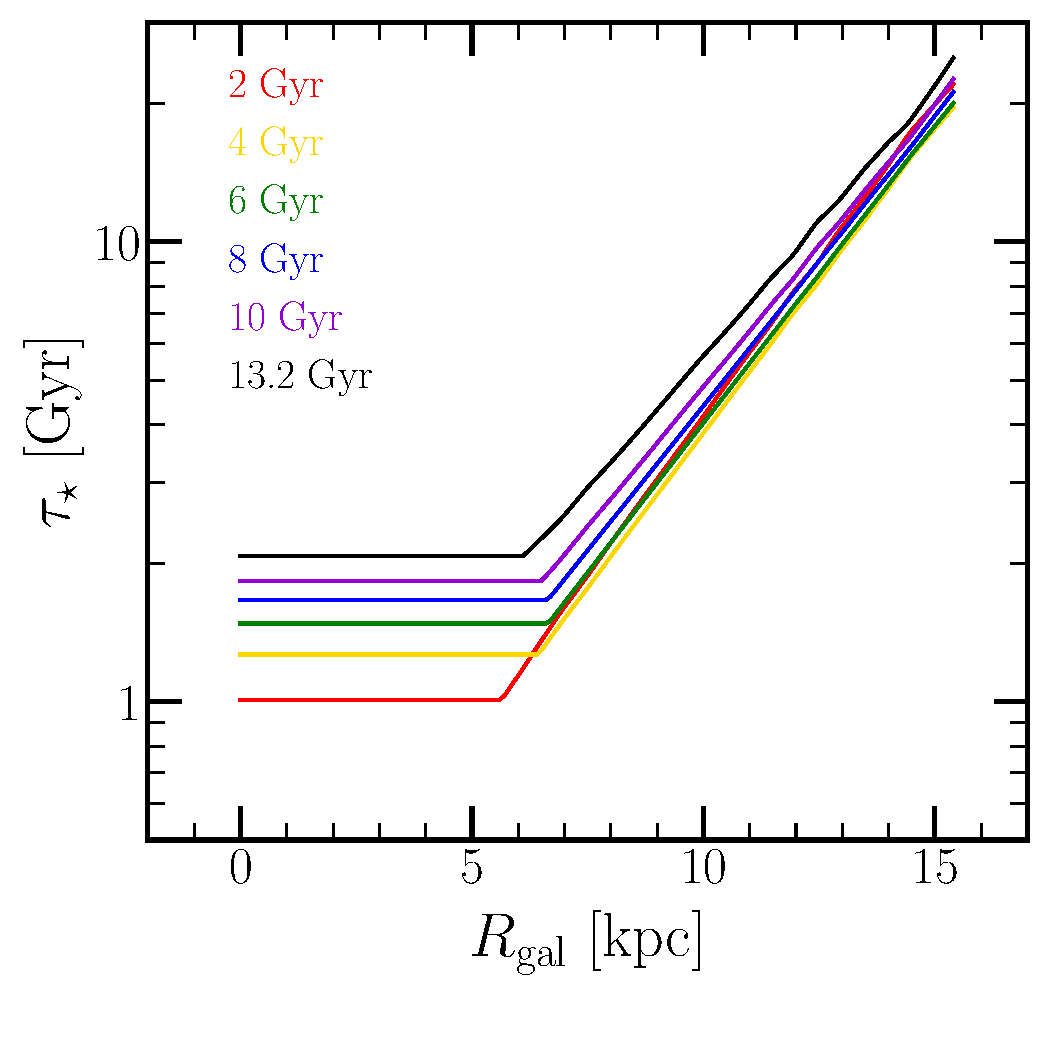
\includegraphics[scale = 0.45]{sfe.pdf} 
\caption{The star formation efficiency timescale~$\tau_\star$ as a function of 
Galactocentric radius at simulation times of 2 Gyr (red), 4 Gyr (yellow), 
6 Gyr (green), 8 Gyr (blue), 10 Gyr (purple), and 13.2 Gyr (the present day, 
black) predicted by our fiducial model. } 
\label{migration:fig:sfe} 
\end{figure} 

\citet{Krumholz2018a} compare theoretically motivated star formation laws to 
the observations of~\citet{Bigiel2010} and~\citet{Leroy2013} (see their Fig. 2). 
We find that the following by-eye fit to the power-law index~$N$~is a 
reasonable description of the aggregate data: 
\begin{equation} 
N = \begin{cases} 
1.0 & (\Sigma_\text{g} \geq \Sigma_{\text{g},2})~, \\ 
3.6 & (\Sigma_{\text{g},1} \leq \Sigma_\text{g} \leq \Sigma_{\text{g},2})~, \\ 
1.7 & (\Sigma_\text{g} \leq \Sigma_{\text{g},1})~, 
\end{cases} 
\label{migration:eq:sf_law_indeces} 
\end{equation} 
where~$\Sigma_{\text{g},1} = 5\times10^6$~\msun~\persqkpc~and 
$\Sigma_{\text{g},2} = 2\times10^7$~\msun~\persqkpc. 
The apparent linearity of the relationship above 
$\sim2\times10^7$~\msun~\persqkpc~suggests that in this regime, star formation 
proceeds at the highest efficiency, and that 
$\tau_\star \equiv \Sigma_\text{g}/\dot{\Sigma}_\star$~= constant. 
The observational results of~\citet{Leroy2013} and~\citet{Kennicutt2021} would 
suggest that these are the surface densities at which the molecular fraction 
$f_\text{mol} = M_{\text{H}_2} / (M_{\text{H}_2} + M_\text{HI}) \approx$~1. 
We therefore adopt the assumption that above 
$\Sigma_\text{g} = 2\times10^7$~\msun~\persqkpc,~$\tau_\star$ reaches its 
minimum value, and increases with decreasing~$f_\text{mol}$. 
We denote this value as~$\tau_\text{mol}$, the value of~$\tau_\star$ for a gas 
reservoir with~$f_\text{mol}$~= 1. 
This identification, combined with our three-component power-law index~$N$ 
results in the following final form for our adopted star formation law: 
\begin{equation} 
\dot{\Sigma}_\star = \begin{cases} 
\Sigma_\text{g} \tau_\text{mol}^{-1} & 
(\Sigma_\text{g} \geq \Sigma_{\text{g},2})~, 
\\ 
\Sigma_\text{g} \tau_\text{mol}^{-1} \left(\frac{
	\Sigma_\text{g}
}{
	\Sigma_{\text{g},2} 
}\right)^{2.6} & 
(\Sigma_{\text{g},1} \leq \Sigma_\text{g} \leq \Sigma_{\text{g},2})~, 
\\ 
\Sigma_\text{g} \tau_\text{mol}^{-1} \left(\frac{
	\Sigma_{\text{g},1} 
}{
	\Sigma_{\text{g},2} 
}\right)^{2.6}\left(\frac{
	\Sigma_\text{g}
}{
	\Sigma_{\text{g},1} 
}\right)^{0.7} & 
(\Sigma_\text{g} \leq \Sigma_{\text{g},1})~. 
\end{cases} 
\label{migration:eq:sf_law} 
\end{equation} 
We choose the power-law indices such that this formalism is consistent 
with equation~\refp{migration:eq:sf_law_indeces}, and prefactors are added to ensure 
piece-wise continuity. 
In implementation,~\vice~requires the~$\tau_\star-\dot{\Sigma}_\star$ relation 
when running in star formation mode and the~$\tau_\star-\Sigma_\text{g}$ 
relation when running in infall and gas modes. 
Both follow algebraically from this relationship given the substitution 
$\tau_\star \equiv \Sigma_\text{g} / \dot{\Sigma}_\star$. 
\par 
Based on the observed Kennicutt-Schmidt relation at different redshifts, 
\citet{Tacconi2018} suggest that~$\tau_\text{mol}$ should scale with redshift 
$z$ and with the deviation from the star forming main sequence~$\delta$MS via 
$\tau_\text{mol} \propto (1 + z)^{-0.6}\delta\text{MS}^{-0.44}$. 
We do not account for the effect of~$\delta$MS in our models, but we do 
incorporate the redshift dependence. 
For redshifts of~$z \lesssim$~3, encompassing most of the timesteps in 
our models, a reasonable approximation to the~$t - z$ relation assuming 
typical~$\Lambda$CDM cosmology is given by: 
\begin{equation} 
\frac{t}{t_0} \approx (1 + z)^{-5/4}, 
\end{equation} 
where~$t_0$ is the present-day age of the universe, and~$t$ is not simulation 
time but the age of the universe. Plugging this relation into the 
\citet{Tacconi2018} scaling yields 
\begin{equation} 
\tau_\text{mol} = \tau_{\text{mol},0}(t/t_0)^{12/25} \approx 
\tau_{\text{mol},0}(t/t_0)^{1/2}, 
\end{equation} 
where~$\tau_{\text{mol},0}$ is simply~$\tau_\text{mol}$ at the present day. We 
generalize this formula to the following form: 
\begin{equation} 
\tau_\text{mol} = \tau_{\text{mol},0}(t/t_0)^\gamma 
\label{migration:eq:tau_mol}
\end{equation} 
In this paper we present models which adopt~$\tau_{\text{mol},0}$ = 2 Gyr 
\citep{Leroy2008, Leroy2013, Tacconi2018} and~$\gamma$ = 1/2 based on this 
argument. 
We have also run simulations witht~$\tau_{\text{mol},0}$ = 1 
Gyr and with~$\gamma$ = 0 (a time-independent~$\tau_\text{mol}$), as well as 
combinations of the two, and found similar results. 
In all timesteps and annnuli,~\vice~infers~$\Sigma_\text{g}$ from 
$\dot{\Sigma}_\star$ given our equations~\refp{migration:eq:sf_law} and~\refp{migration:eq:tau_mol}. 
\par
In Fig.~\ref{migration:fig:sfe}, we plot~$\tau_\star$ as a function of~$\rgal$ at 
six different time stamps predicted by our fiducial, inside-out SFH model. 
At~$\rgal \lesssim$ 6 kpc,~$\tau_\star$ is near~$\tau_\text{mol}$ at all 
times, implying a molecular fraction of unity at these radii. 
Although this prediction is likely unrealistic because 21-cm line observations 
suggest the presence of neutral hydrogen as close to the Galactic centre as 
several hundred pc~\citep{Kalberla2009}, we find in practice that changing our 
assumptions about the star formation law does not impact our conclusions. 
In exploratory work for this paper, we investigated purely linear, purely 
power-law, and broken power-law characterizations, finding similar predictions 
in all cases. 
In general we find that the detailed form of the SFH, and to some extent the 
time-dependence of radial migration, exert much greater power in establishing 
the model predictions than does the star formation law. 
Nonetheless it is an interesting puzzle that a 
$\dot{\Sigma}_\star - \Sigma_\text{g}$ relation informed by the observed 
population-averaged trends and the normalization of SFHs implied by the stellar 
mass of the Milky Way predicts results in tension with the observed HI 
distribution. 
Because the star formation law has minimal impact on our results, we do not 
pursue this question further here. 

\subsection{Surface Density Gradient} 
\label{migration:sec:methods:surface_density_gradient} 

\afterpage{
\clearpage
\small
\begin{landscape}
\begin{table*}
\caption{
A summary of our chemical evolution model parameters, their fiducial values,
and in what section of the text relevant discussion can be found.
}
\begin{tabularx}{\linewidth}{l @{\extracolsep{\fill}} l l r}
\hline
\hline
Quantity & Section & Description & Fiducial Value(s)
\\
\hline
\rgal & N/A & Galactocentric Radius & $0 - 20$ kpc
\\
$\delta$\rgal & \ref{migration:sec:methods:summary} & Width of each concentric
ring &  100 pc
\\
$\Delta$\rgal & \ref{migration:sec:methods:migration} & Change in orbital
radius due to stellar migration & N/A
\\
\null & \null & (adopted from~\hsim~analogue star particle) & \null
\\ 
$z$ & \ref{migration:sec:methods:migration} & Present day distance to Galactic
midplane & [$-3$, 3] kpc
\\
\null & \null & (adopted from~\hsim~analogue star particle) & \null
\\ 
$T_\text{max}$ & \ref{migration:sec:methods:h277} & Time interval over which
our models are integrated & 13.2 Gyr
\\
$\delta T$ & \ref{migration:sec:methods:summary} & Timestep size & 10 Myr 
\\ 
$n$ & \ref{migration:sec:methods:summary} & Number of stellar populations
formed per ring per timestep & 8 
\\ 
$R_\text{SF}$  & \ref{migration:sec:methods:summary} & Maximum radius of star
formation (i.e.~$\dot{\Sigma}_\star$ = 0 at~\rgal~>~$R_\text{SF}$) & 15.5 kpc 
\\ 
$\tau_\star$ & \ref{migration:sec:methods:sfe} & The SFE timescale of the ISM: 
$\tau_\star \equiv \Sigma_\text{gas} / \dot{\Sigma}_\star$ & N/A 
\\ 
$\tau_{\text{mol},0}$ & \ref{migration:sec:methods:sfe} & The SFE timescale of
molecular hydrogen at the present day & 2 Gyr 
\\ 
$\gamma$ & \ref{migration:sec:methods:sfe} & The power-law index describing the 
time-dependence of the molecular & 1/2
\\
\null & \null & hydrogen SFE timescale
(i.e.~$\tau_\text{mol}\sim t^\gamma$) & \null
\\ 
$\eta$ & \ref{migration:sec:methods:outflows} & The outflow mass-loading
factor: $\eta \equiv \dot{\Sigma}_\text{out}/\dot{\Sigma}_\star$ &
equation~\refp{migration:eq:eta_rgal}
\\
\null & \null & (assumed to be time-independent) & \null
\\ 
$y_\text{O}^\text{CC}$ & \ref{migration:sec:methods:yields} & CCSN yield of O &
0.015 
\\ 
$y_\text{Fe}^\text{CC}$ & \ref{migration:sec:methods:yields} & CCSN yield of
Fe & 0.0012 
\\ 
$y_\text{O}^\text{Ia}$ & \ref{migration:sec:methods:yields} & SN Ia yield of O
& 0 
\\ 
$y_\text{Fe}^\text{Ia}$ & \ref{migration:sec:methods:yields} & SN Ia yield of
Fe & 0.00214 
\\ 
$\dot{\Sigma}_\star$ & \ref{migration:sec:methods:sfhs} & Surface density of
star formation & N/A
\\ 
$f_\text{IO}(t|\rgal)$ & \ref{migration:sec:methods:sfhs} & The time-dependence
of the star formation history in the inside-out
model & equation~\refp{migration:eq:insideout_sfh} 
\\ 
$f_\text{LB}(t|\rgal)$ & \ref{migration:sec:methods:sfhs} & The time-dependence
of the  star formation history in the late-burst
model & equation~\refp{migration:eq:lateburst_sfh} 
\\ 
\hline 
\end{tabularx} 
\label{migration:tab:params} 
\end{table*}
\end{landscape}
\clearpage
}

% As discussed in~\S~\ref{migration:sec:methods:sfhs}, Appendix~\ref{migration:sec:normalize_sfh} 
% presents the recipe by which we select a unitless function describing the 
% stellar surface density gradient~$g(\rgal)$. 
% {\color{red} 
As discussed in~\S~\ref{migration:sec:methods:sfhs}, Appendix~\ref{migration:sec:normalize_sfh} 
presents the recipe by which we normalize our star formation histories, a 
necessary component of which is a unitless function describing the stellar 
surface density gradient~$g(\rgal)$. 
% }
In setting the normalization, our model ensures that the integral of~$g(\rgal)$ 
over the surface area of the disc predicts a total stellar mass in agreement 
with that observed for the Milky Way. 
For this value, we adopt~$M_\star^\text{MW} = 5.17~\times~10^{10}~\msun$ from 
\citet[][$\pm 1.11\times10^{10}~\msun$]{Licquia2015}. 
This is the total disc mass only; when the bulge is included, the total 
becomes~$(6.08~\pm~1.17)~\times~10^{10}~\msun$. 
Since we are modeling only the disc populations here, we omit the contribution 
from the bulge to the total mass budget. 
% For this value, we adopt 
% $M_\star^\text{MW} = (5.17 \pm 1.11)\times10^{10}$~\msun~\citep{Licquia2015}. 
% This is the total disc mass of the Galaxy;~\citet{Licquia2015} report 
% $(6.08 \pm 1.17)\times10^{10}~\msun$~when the bulge is considered. 
% Since we are modeling only the disc populations here, we omit the contribution 
% the bulge would have to the total mass budget. 
% This is the total stellar mass of the Galaxy, including the bulge; 
% \citet{Licquia2015} report~$(5.17 \pm 1.11)\times10^{10}$~\msun~as the mass of 
% the disc alone. 
% Although we are not modeling the bulge here, our model extends to~$\rgal$ = 0 
% and our sample of candidate analogue star particles from~\hsim includes those 
% with bulge-like kinematics. 
\par 
We adopt a double exponential form for~$g(\rgal)$, describing the thin and 
thick disc components of the Galaxy: 
\begin{equation} 
g(\rgal) = e^{-\rgal/R_t} + \frac{\Sigma_T}{\Sigma_t} 
e^{-\rgal/R_T}~, 
\label{migration:eq:gradient} 
\end{equation} 
where~$R_t$~and~$R_T$~are the scale radii of the thin and thick discs, 
respectively, and~$\Sigma_T/\Sigma_t$~is the ratio of their surface densities 
at~$\rgal$~= 0. 
We adopt~$R_t$~= 2.5 kpc,~$R_T$~= 2.0 kpc, and~$\Sigma_T/\Sigma_t$~= 0.27 based 
on the findings of~\mbox{\citet{Bland-Hawthorn2016}}. 
We plot the single exponential forms of each disc component as dotted black 
lines in Fig.~\ref{migration:fig:surface_density}, with the solid black line denoting the 
sum of the two. 

% fig 6 
\begin{figure} 
\centering 
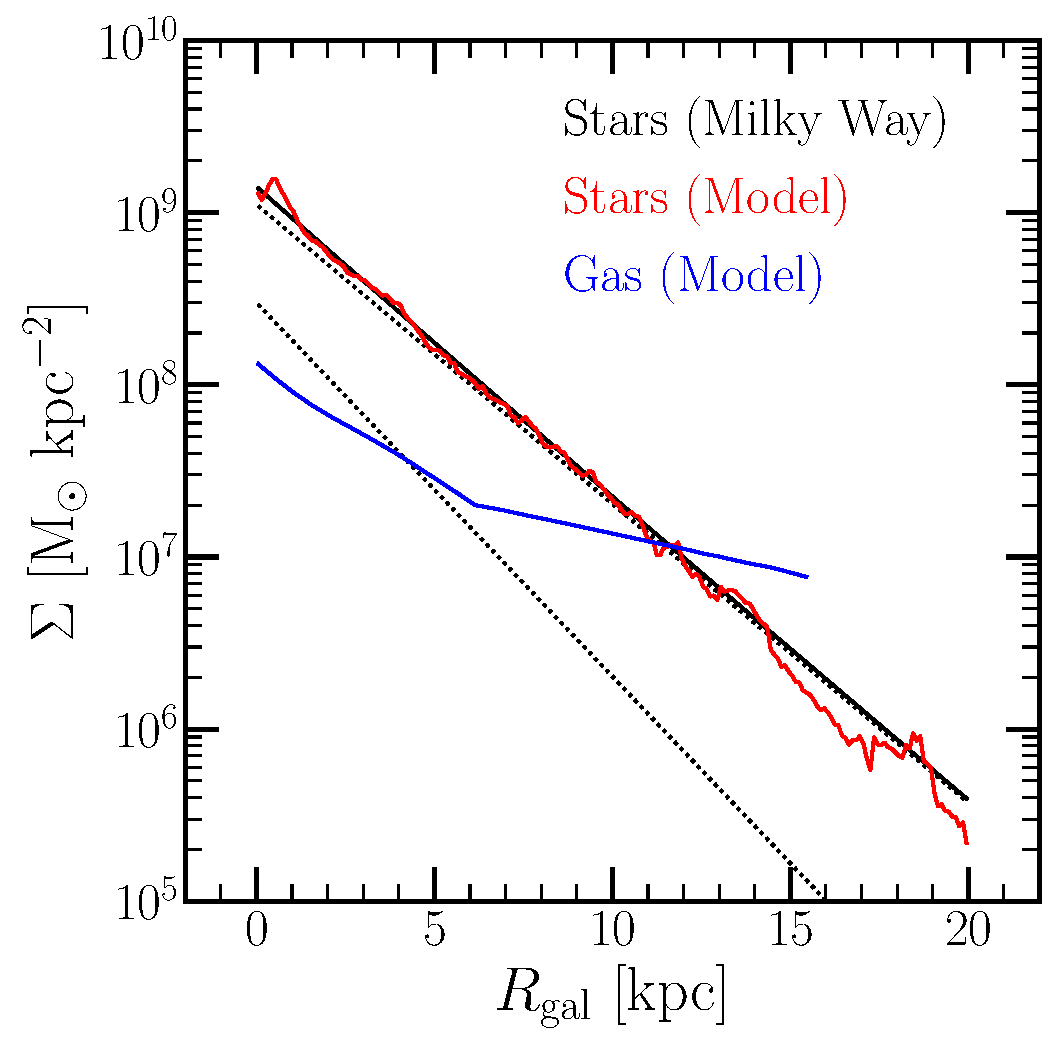
\includegraphics[scale = 0.45]{surface_density_gradient.pdf} 
\caption{The surface density of gas (blue) and stars (red) as predicted by our 
fiducial model. The dotted black lines denote thin and thick disc 
profiles with scale lengths of~$R_t$ = 2.5 kpc and~$R_T$ = 2.0 kpc, 
respectively, with a ratio of~$\Sigma_T/\Sigma_t$ = 0.27 at~\rgal~= 0 (i.e. the 
thin disc profile has the higher normalization). 
The solid black line denotes the sum of the two; this is the stellar surface 
density gradient of the Milky Way as reported by~\citet{Bland-Hawthorn2016}, 
renormalized according to our adopted total stellar mass of 
$(5.17 \pm 1.11)\times10^{10}$~\msun~\citep{Licquia2015}. } 
\label{migration:fig:surface_density} 
\end{figure} 

We plot the resultant surface density gradients from our fiducial, inside-out 
SFH model in Fig.~\ref{migration:fig:surface_density} as well, with red denoting the 
stellar gradient and the gas in blue. 
The stellar gradient very nearly follows our target gradient (equation 
\ref{migration:eq:gradient}) denoted by the solid black line. 
% {\color{red} 
Simply introducing scatter around the adopted trend, stellar migration has 
not significantly altered the overall form of the gradient, as we assumed in 
Appendix~\ref{migration:sec:normalize_sfh}. 
We find this to also be true for our sample of star particles from~\hsim, 
a result which is expected given the roughly symmetric shapes of the 
histograms in the top row of Fig.~\ref{migration:fig:h277_decomposition} and consistent 
with previous arguments that radial migration does not significantly alter the 
vertical and radial structure of the disc~\citep[e.g.][]{Sellwood2014, 
VeraCiro2014}. 
% }
% Stellar migration has not altered the overall form of the gradient, simply 
% introducing scatter around the adopted trend. 
Although there are slight enhancements at small~$\rgal$ and deficits at large 
$\rgal$, the agreement is excellent in the regions of the Galaxy where the 
gradient is best constrained observationally. 
The~$\rgal$ > 15.5 kpc populations are composed entirely of stars that 
migrated there, since that is the radius at which we shut off star formation. 
The gas gradient shows a break in the scale radius near~$\rgal \approx$ 
6 kpc. This is a consequence of our adopted star formation law; at 
$\Sigma_\text{g} = 2\times10^7$~\msun~\persqkpc~the relation changes from 
linear at higher densities to~$\dot{\Sigma}_\star \sim \Sigma_\text{g}^{3.6}$ 
at lower densities (see discussion in~\S~\ref{migration:sec:methods:sfe}). 
\par 
Although we adopt the~\citet{Licquia2015} disc stellar mass of the Milky Way 
here, we find similar results when taking a value which differs even by an 
order of magnitude. 
If we used a linear star formation law, then our chemical evolution would be 
independent of the mass normalization as it is in corresponding one-zone 
models (\citealp*{Spitoni2017};~\citealp{Weinberg2017b, Belfiore2019}). 
The mass normalization enters our calculation because it affects the transition 
between the linear and non-linear regimes of our star formation law 
(equation~\ref{migration:eq:sf_law}), but the impact on abundance evolution is minimal. 

\subsection{Summary} 
\label{migration:sec:methods:summary} 

% fig 7 
\afterpage{
\clearpage
\begin{landscape}
\begin{figure*} 
\centering 
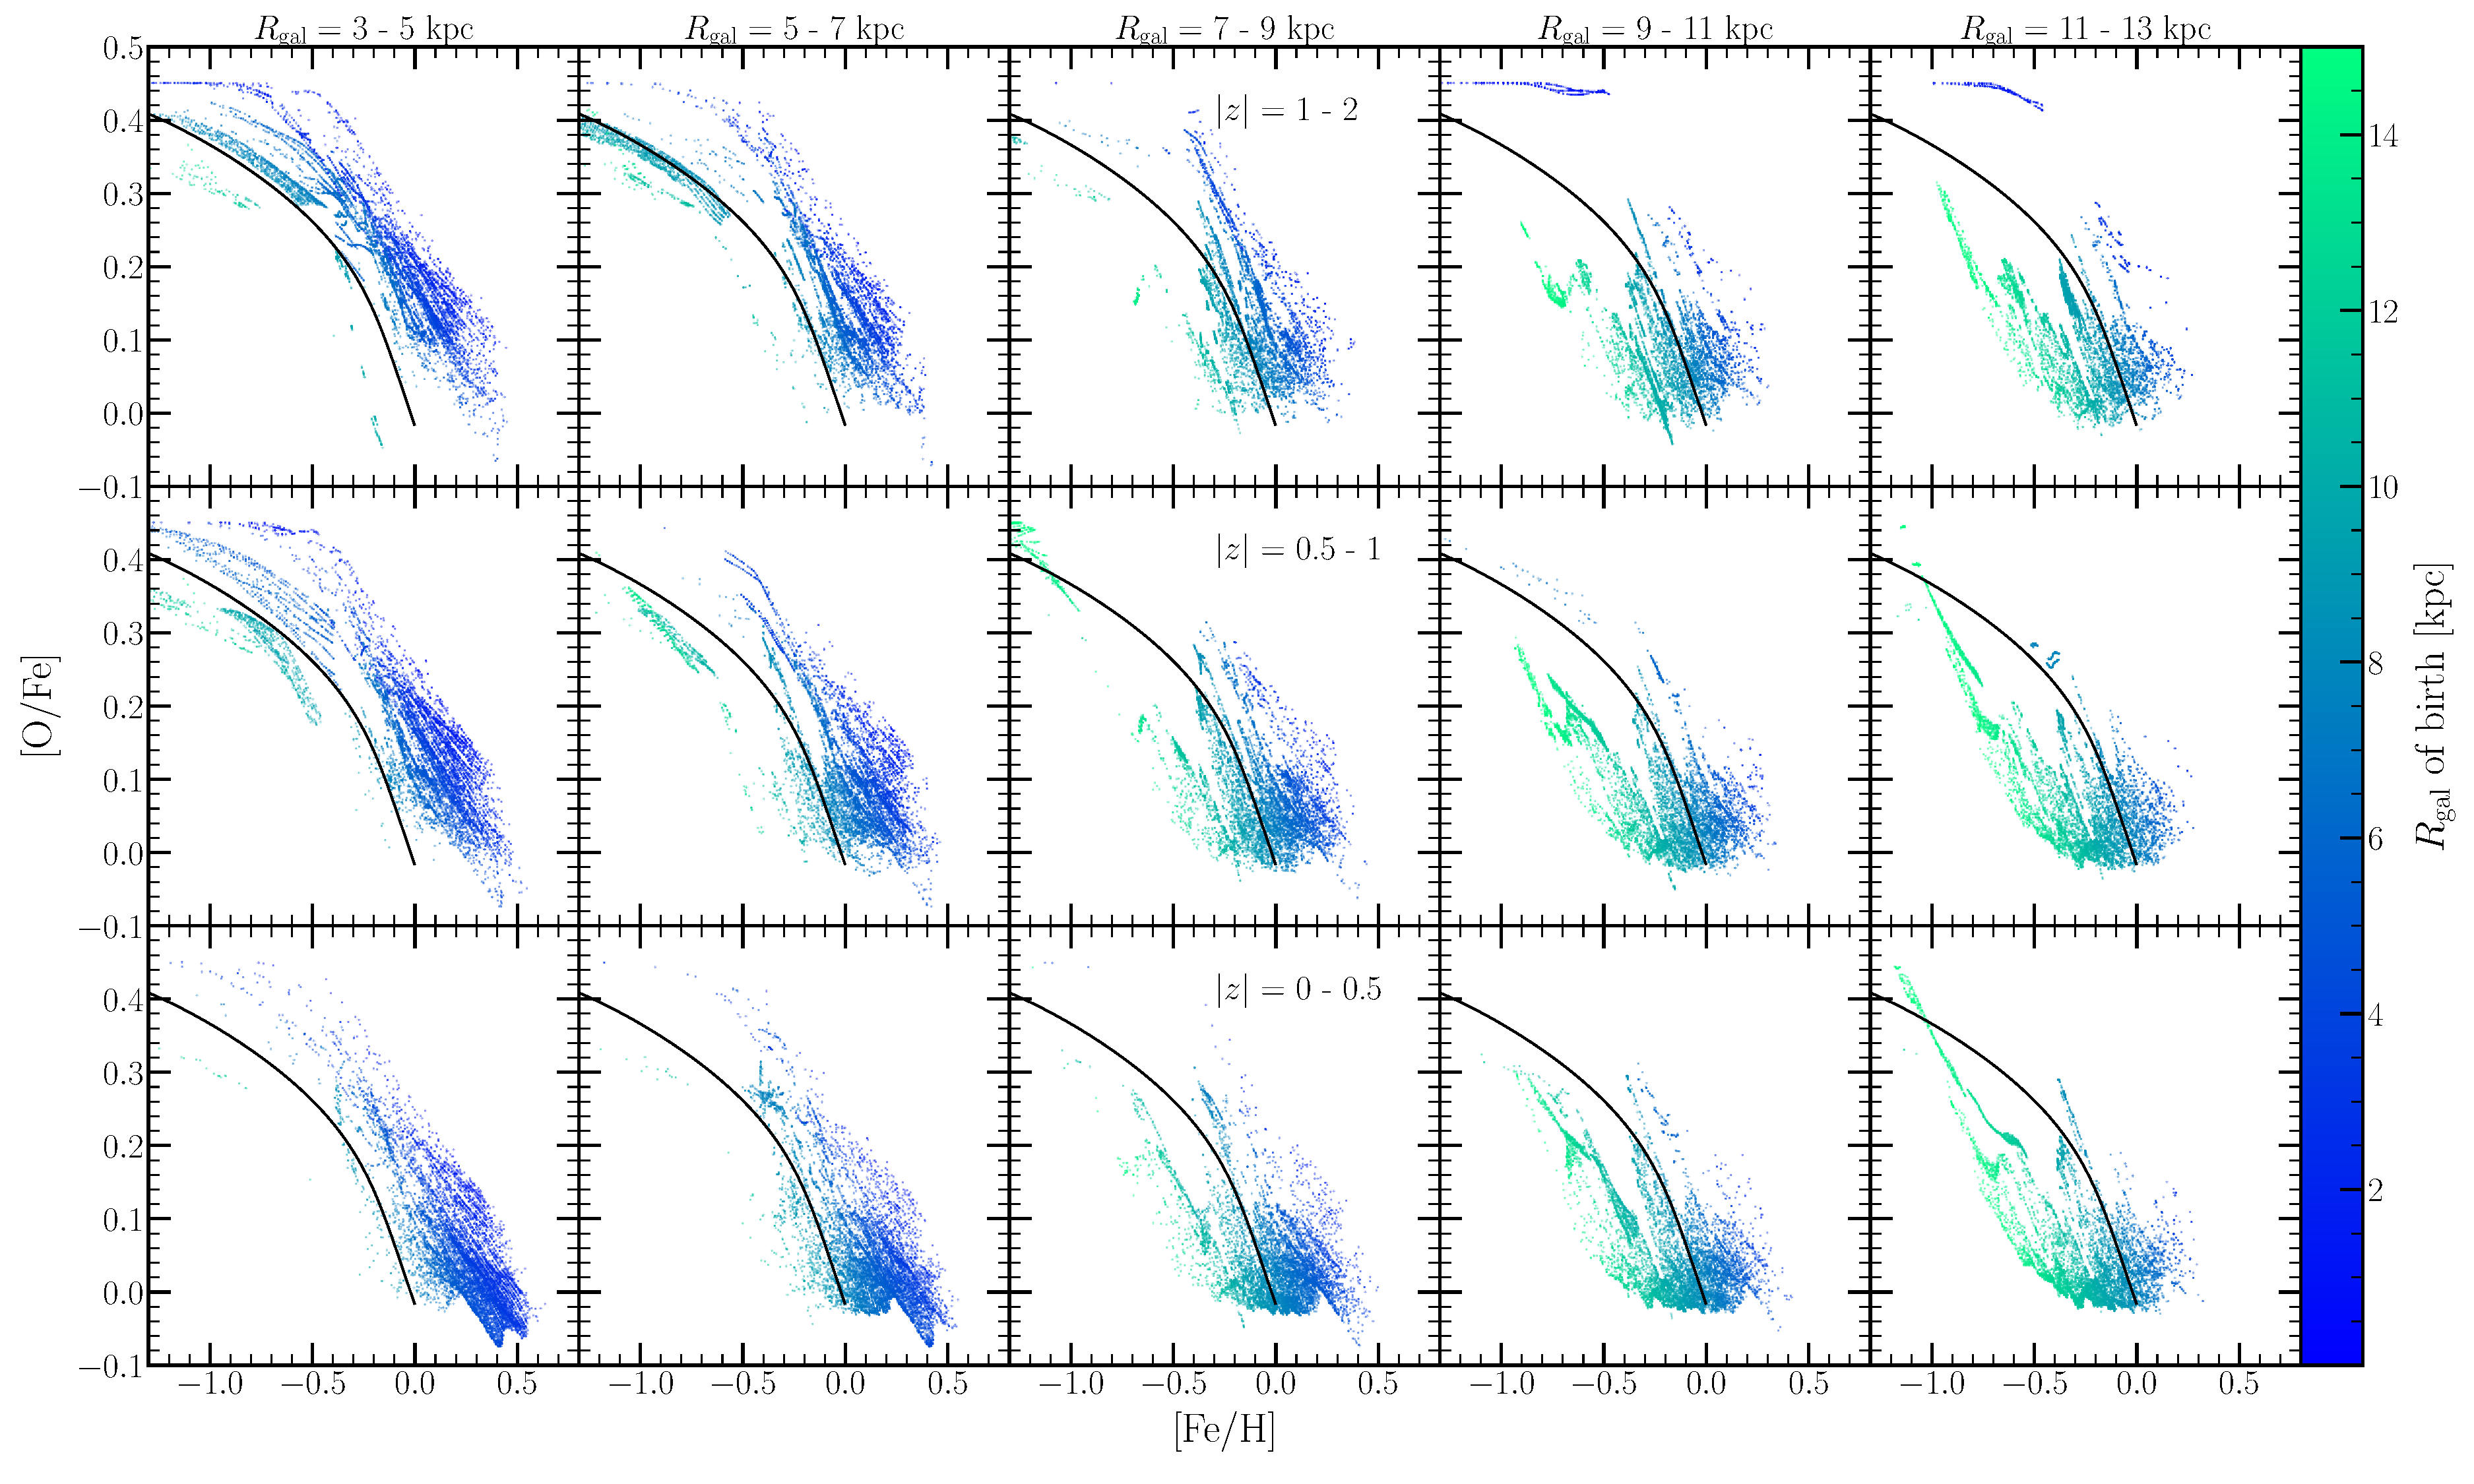
\includegraphics[scale = 0.3]{ofe_feh_densitymap.pdf} 
\caption{[O/Fe]-[Fe/H] diagrams for 15 Galactic regions spanning five bins in 
$R_\text{gal}$ and three in~$\left|z\right|$. Each region has its own panel, 
with radial bins shown in columns denoted at the top, and with bins in 
$\left|z\right|$ shown in rows denoted in text in the middle column. For each 
region, we plot~$N$~= 10,000 points sampled from our simulated stellar 
populations predicted by our fiducial model, where the probability of 
sampling is proportional to the present-day mass of each stellar population. 
In all panels, points are colour-coded according to the Galactocentric radius 
of birth of the stellar population. For reference, we plot in a solid black 
line in all panels the gas-phase [O/Fe]-[Fe/H] track predicted by the same 
SFH in the~$R_\text{gal}$ = 8 kpc annulus, but with the post-processing 
migration model; this curve is the same in all panels. } 
\label{migration:fig:ofe_feh_diagram} 
\end{figure*} 
\end{landscape}
\clearpage
}

% {\color{red} 
Table~\ref{migration:tab:params} presents a breakdown of our model parameters, their 
values, and references to the sections where relevant discussion can be found. 
% }
In summary, our fiducial model has an inside-out SFH with e-folding timescales 
derived from the observations of~\citet[][see discussion 
in~\S~\ref{migration:sec:methods:sfhs}]{Sanchez2020}. 
Radial migration proceeds in a manner in which our model stellar populations 
have a change in radius~$\Delta \rgal$ informed from the~\texttt{h277} 
hydrodynamical simulation~\citep[][see discussion 
in~\S~\ref{migration:sec:methods:h277}]{Christensen2012, Zolotov2012, Loebman2012, 
Loebman2014, Brooks2014}. 
In the baseline model, stars move to their final radius with a 
$\sqrt{\text{age}}$~dependence~\citep[][see discussion in 
\ref{migration:sec:methods:migration}]{Frankel2018,Frankel2020}. 
Using~\vice~to calculate abundances for O and Fe in this paper, our supernova 
yields are adopted from~\citet{Johnson2020}, who in turn take these values from 
\citet{Weinberg2017b} (see~\S~\ref{migration:sec:methods:yields}). 
Outflows are characterized such that the equilibrium abundance of oxygen under 
a constant SFH follows an abundance gradient in agreement with observational 
results in the Milky Way (see~\S~\ref{migration:sec:methods:outflows}). 
Our star formation law is based on the~\citet{Bigiel2010} and 
\citet{Leroy2013} data presented in comparison with theoretical models in 
\citet[][see~\S~\ref{migration:sec:methods:sfe}]{Krumholz2018a}. 
To describe the stellar surface density gradient, we adopt the two-exponential 
form describing the thin and thick discs from 
\citet[][see~\S~\ref{migration:sec:methods:surface_density_gradient}]{Bland-Hawthorn2016}. 
We adopt the~\citet{Kroupa2001} IMF throughout this paper. 
\par 
Our selection of star particles from~\hsim~yields a sample of 1,751,765 
candidate analogues with disc-like kinematics at the present day (see 
discussion in~\S~\ref{migration:sec:methods:h277}). 
We take~$\delta\rgal$ = 100 pc as the width of each annulus from~\rgal~= 0 to 
20 kpc and a timestep size of~$\delta T$ = 10 Myr from~$T$ = 0 to 13.2 Gyr. 
With the resulting 200 zones and 1,321 timesteps (one extra so that age = 0 
stars are included), we let~\vice~form~$n$ = 8 stellar populations per zone per 
timestep, resulting in 2,113,600 total stellar populations with predicted 
masses and abundances. 
We set the SFR to zero beyond~\rgal~= 15.5 kpc; stellar populations 
do form beyond this radius and are part of the computational overhead, but they 
have zero mass and thus do not contribute to the chemical evolution in our 
models. 
This results in 1,627,472 stellar populations with~\textit{non-zero} masses and 
abundances, comparable to the total number of disc particles in our sample 
from~\hsim. 
These simulations run in~$\sim$5 hours on a single core with a 3 GHz 
processor and take up~$\sim$235 MB of disc space per output, including the 
extra data that we record for each stellar population's analogue star particle. 
We have also run variations with~$n$ = 2 stellar populations per 
zone per timestep, finding similar results in all cases. 
\par 
We have run~\vice~for all four of our SFHs, all four migration 
models, and all four variations in~$\tau_\text{mol}$ noted 
in~\S~\ref{migration:sec:methods:sfe} --- a total of 64 simulations, as well as a variety 
of other test cases. 
For many of our results, only the SFH variations have a substantial impact. 
We discuss the impact of migration or~$\tau_\text{mol}$ variations where they 
are relevant. 



\section{Comparison to Observations} 
\label{migration:sec:obs_comp} 

% fig 8
\afterpage{
\clearpage
\begin{landscape}
\begin{figure*} 
\centering 
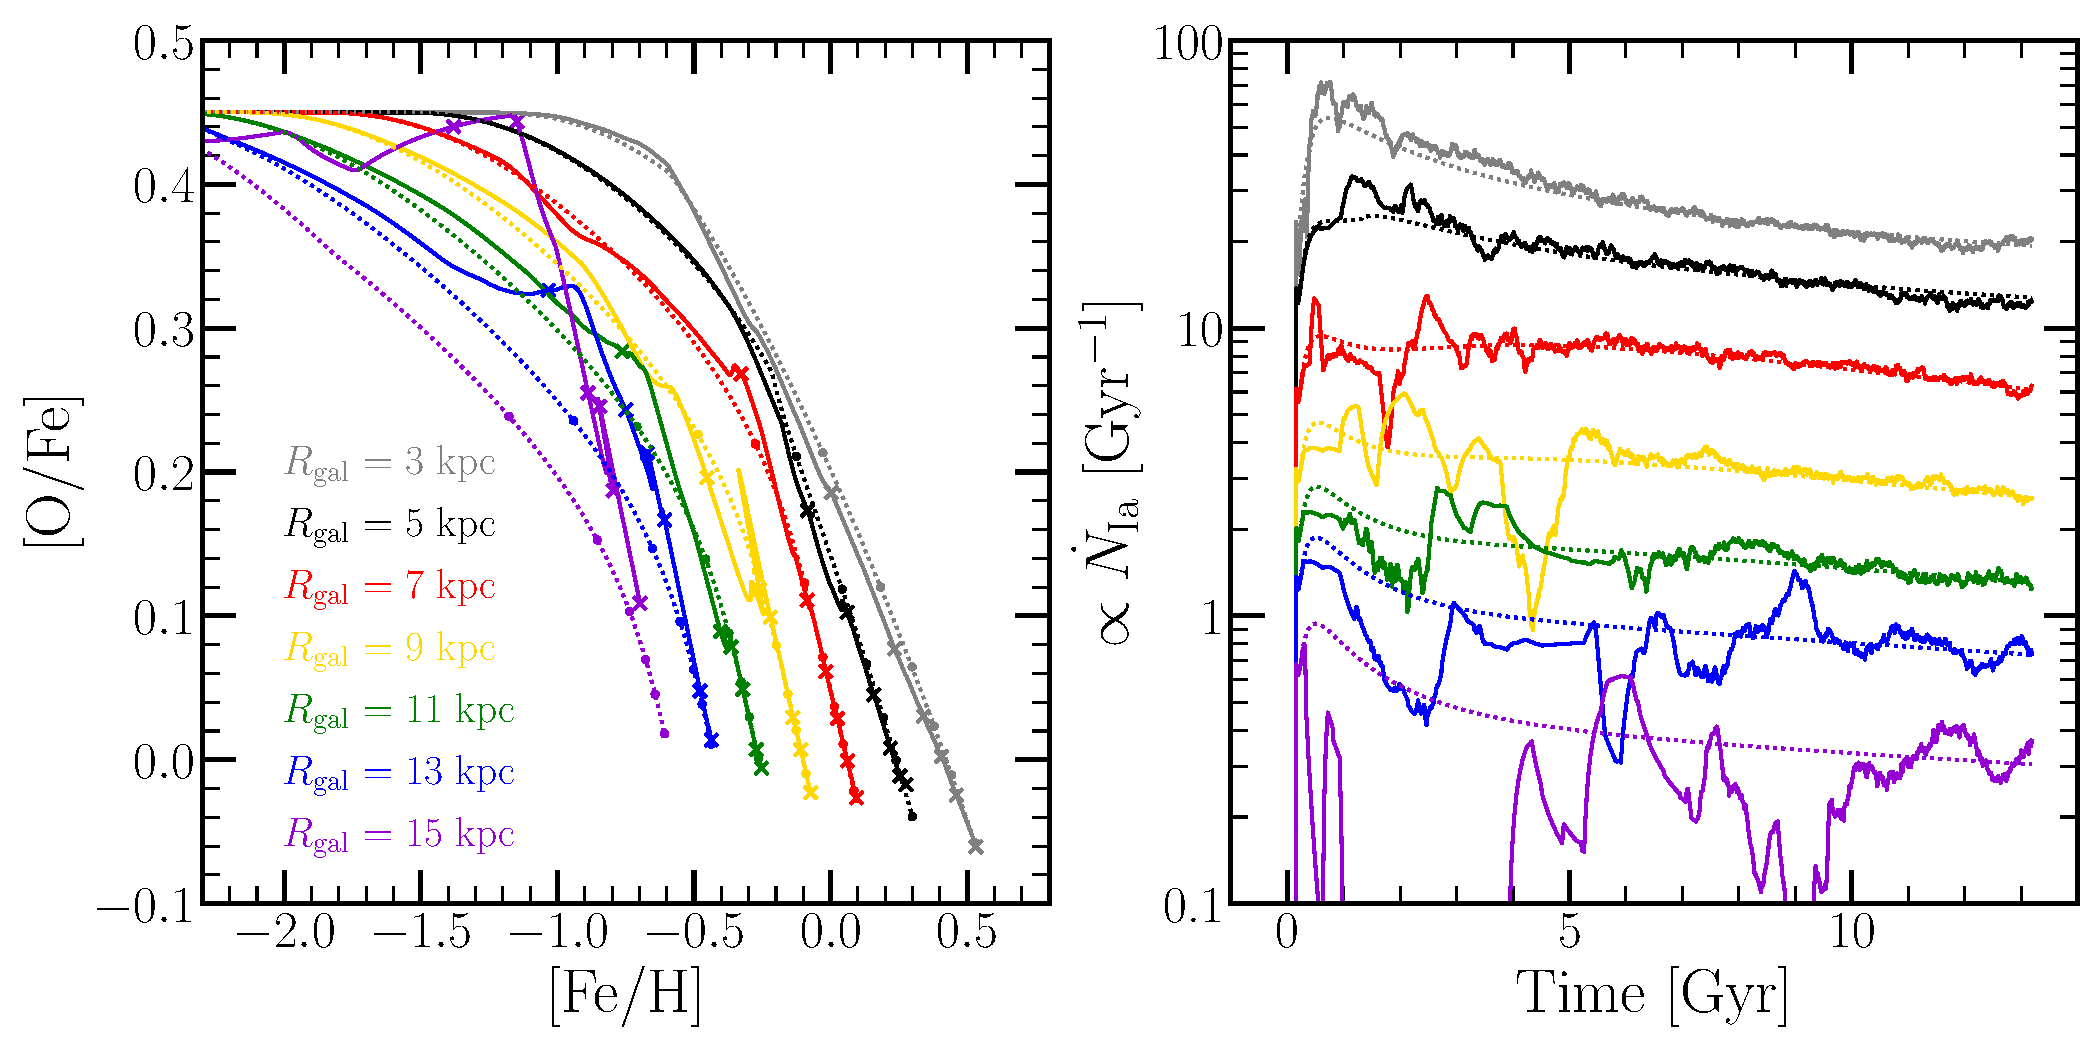
\includegraphics[scale = 0.47]{tracks.pdf} 
\caption{\textbf{Left}: Gas phase evolutionary tracks in the [O/Fe]-[Fe/H] 
plane for our inside-out SFH with either post-processing (dotted lines) or 
diffusion (solid lines) migration models. We plot tracks for seven of our 
$\delta\rgal$ = 100 pc rings, 
colour-coded according to their Galactocentric radius and denoted by the 
legend in the lower-left. We mark simulation times of 2, 4, 6, 8, 10, and 13.2 
Gyr in X's for the diffusion model and points for the post-processing model. 
\textbf{Right}: As a function of simulation time, a proxy for the SN Ia rate 
using the total time-derivative of the Fe mass in a given annulus, calculated 
by subtracting the contribution from recycling and CCSN enrichment and adding 
back that lost to star formation and outflows. We show these rates for the 
same rings as in the left-hand panel, multiplying them by various prefactors 
to improve clarity. } 
\label{migration:fig:tracks} 
\end{figure*} 
\end{landscape}
\clearpage
}

We begin the comparison of our model predictions to observational data with the 
distribution of stellar populations in the [O/Fe]-[Fe/H] plane. We separate 
stars into bins based on their present-day Galactic regions defined by five 
bins in~$R_\text{gal}$ (3 - 5, 5 - 7, 7 - 9, 9 - 11, and 11 - 13 kpc) and three 
bins in~$\left|z\right|$ (0 - 0.5, 0.5 - 1, and 1 - 2 kpc). Within each of the 
resulting 15 regions, we sample 10,000 stars at random from our baseline 
inside-out SFH model. Since stars in~\texttt{VICE} are stand-ins for entire 
stellar populations, we let the probability of sampling one of them be 
proportional to its present day mass. We plot the results of this procedure in 
Fig.~\ref{migration:fig:ofe_feh_diagram}, colour-coding each stellar population by its 
birth radius; for visual reference, we also plot the gas-phase track which 
resulted from the~$R_\text{gal}$ = 8 kpc annulus with the post-processing 
migration model in a black solid line in all panels. 
\par 
In Fig.~\ref{migration:fig:ofe_feh_diagram}, we note that high-$\alpha$~sequence stars 
are predicted to be the dominant population at small~$R_\text{gal}$ and high 
$\left|z\right|$; conversely, the low-$\alpha$~population dominates the 
statistics at large~$R_\text{gal}$~and low~$\left|z\right|$. This is consistent 
with the observational results of~\citet{Hayden2015}, who present a density map 
in the [$\alpha$/M]-[M/H] plane for the same Galactic regions (see their Fig. 
4).\footnote{
	In~\citet{Hayden2015}, [M/H] represents an overall scaling of elements with 
	solar mixture, and [$\alpha$/M] represents a scaling of~$\alpha$-elements 
	with respect to others. To a good approximation they are proxies for 
	[Fe/H] and [O/Fe], respectively, and we will treat them as such in this 
	paper. 
} 
Furthermore, the locus of the low-$\alpha$ sequence shifts from super-solar 
[Fe/H] to sub-solar [Fe/H] with increasing~$R_\text{gal}$, a shift which is 
expected given the abundance gradient that we have built into our models (see 
discussion in~\S~\ref{migration:sec:methods:outflows}). 
The colour-coding of the points 
shows that the width of the low-$\alpha$~sequence arises out of 
stellar migration: low-$\alpha$ stars with high [Fe/H] formed in the inner 
Galaxy, and those with low [Fe/H] formed in the outer Galaxy. 
The low-$\alpha$ locus thus represents a superposition of populations achieved 
by radial migration rather than an evolutionary sequence, the interpretation 
proposed by, e.g.,~\citet{Schoenrich2009a} and~\citet{Nidever2014}. 
\par 
In Fig.~\ref{migration:fig:ofe_feh_diagram} one can clearly see the imprint of 
evolutionary tracks from different radii, appearing in the same present-day 
$R_\text{gal}$ bin because of radial mixing. 
Though this is to some extent a consequence of the discretization of the 
Galaxy disc in our model, it also arises out of correlated fluctuations in the 
SN Ia rate (see discussion in~\S~\ref{migration:sec:obs_comp:gradient}). 
Observational scatter would wash out the appearance of distinct tracks, and 
intrinsic scatter might blur them if our chemical evolution model was less 
idealized. 
Our model reproduces several of the qualitative trends found by 
\citet{Hayden2015}, but the distribution is less obviously bimodal. 
We quantify this point in~\S~\ref{migration:sec:obs_comp:ofe_dists} below. 
If we remake Fig.~\ref{migration:fig:ofe_feh_diagram} for any of our other SFHs, or for 
our alternative migration or star formation efficiency prescriptions, the 
appearance is qualitatively similar. There are significant quantitative 
differences in some cases, which we discuss in subsequent subsections. 

\subsection{Abundance Gradients} 
\label{migration:sec:obs_comp:gradient} 

% fig 9 
\afterpage{
\clearpage
\begin{landscape}
\begin{figure*} 
\centering 
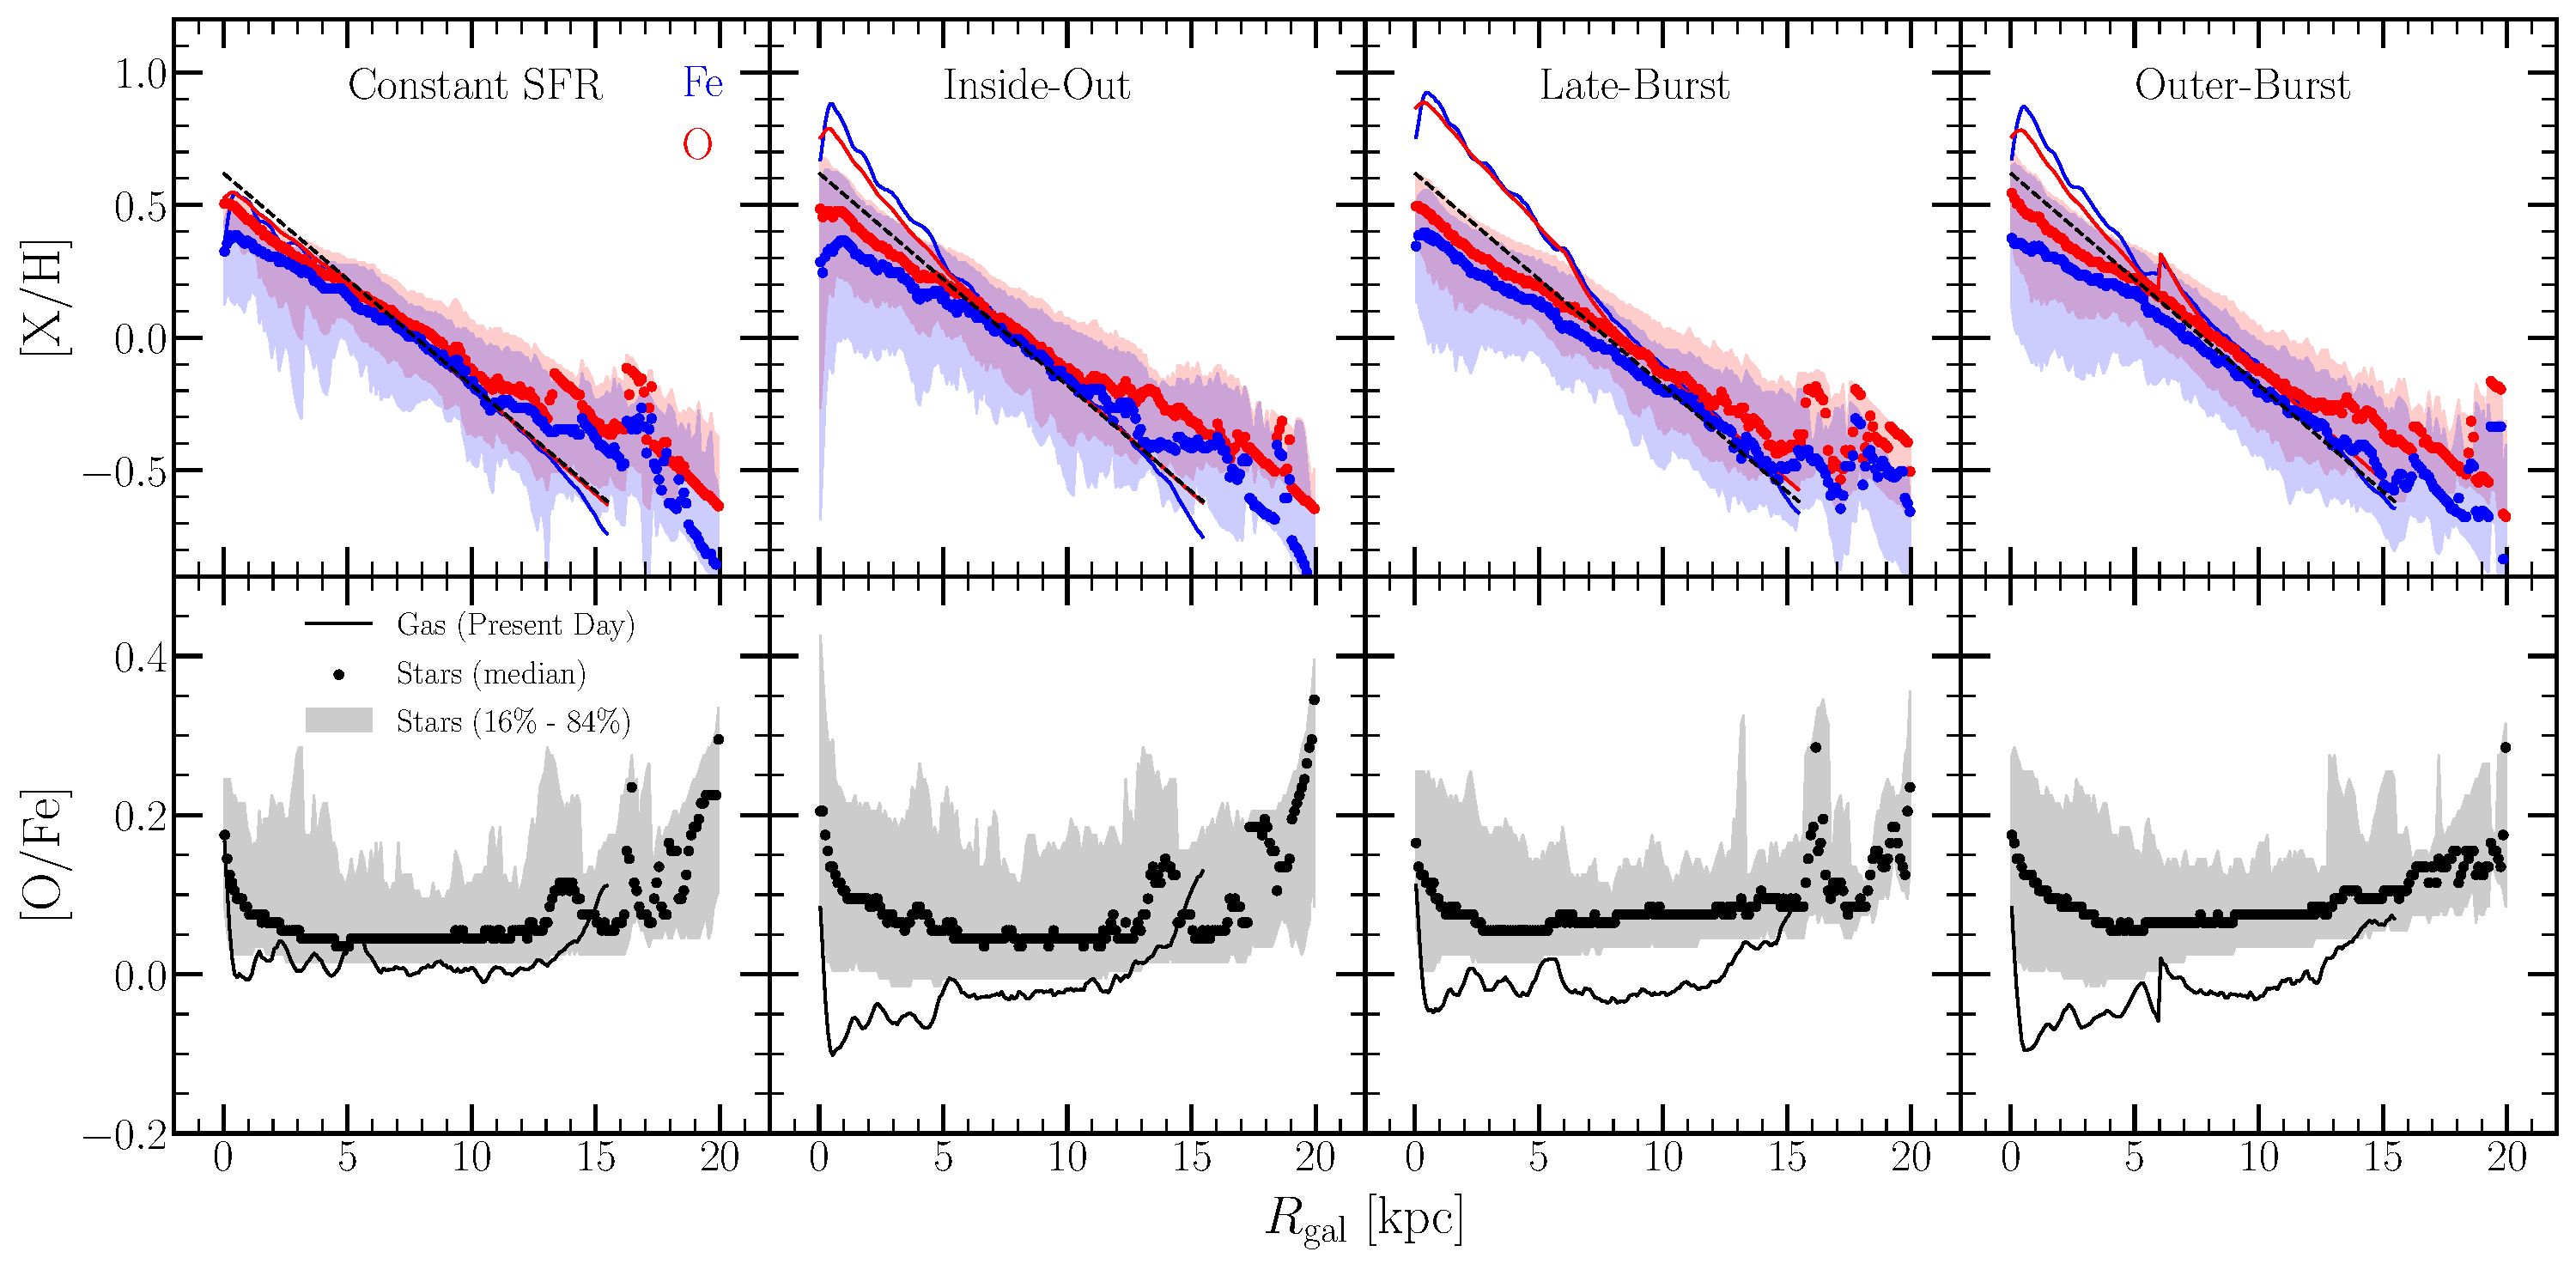
\includegraphics[scale = 0.38]{metallicity_gradient.pdf} 
\caption{Radial abundance gradients in [O/H] (top, red), [Fe/H] (top, blue), 
and [O/Fe] (bottom) for our four SFHs with diffusion migration - constant (far 
left), inside-out (left-middle), late-burst (right-middle), and outer-burst 
(far right). We plot the gas-phase abundance at the present day as a function 
of Galactocentric radius in solid lines. Points denote the median of the stellar 
MDF of the 100-pc width ring at a given radius, with shaded regions marking 
the 16th and 84th percentiles thereof. Black lines in the top panels denote our 
target [$\alpha$/H] gradient of mode([$\alpha$/H]) = +0.3 at~$R_\text{gal}$~= 
4 kpc with a slope of -0.08 kpc$^{-1}$. } 
\label{migration:fig:metallicity_gradient} 
\end{figure*} 
\end{landscape}
\clearpage
}

The left panel of Fig.~\ref{migration:fig:tracks} shows gas phase [O/Fe]-[Fe/H] 
evolutionary tracks at several radii assuming the inside-out SFH, using either 
our post-processing (dotted) or diffusion (solid) migration prescriptions 
(see~\S~\ref{migration:sec:methods:migration} and Fig.~\ref{migration:fig:migration_schema}). 
For the post-processing model the tracks are smooth and simply follow the 
predictions of one-zone GCE models with the parameters appropriate to each 
radius --- with post-processing, radial migration has no impact on the gas-phase 
evolution. 
However, some of the tracks in the diffusion model are notably 
different, especially at early times and large radii. 
These differences arise because radial migration can transport stars 
significantly over the timescale of SN Ia enrichment, as discussed in~\S 
\ref{migration:sec:methods:h277}.
\par 
To demonstrate this point, the right panel of Fig.~\ref{migration:fig:tracks} plots a 
proxy of the SN Ia rate\footnote{
	From our~\vice~outputs, the total time derivative of the Fe mass in a given 
	annulus can be obtained by its change across a single timestep. By then 
	subtracting the CCSN contribution (known exactly given our adopted yield 
	and the SFR), approximately correcting for recycling, and adding back that 
	which was lost to star formation and outflows, we obtain a simple estimate 
	of Fe production by SNe Ia. 
} as a function of time for the same 0.1 kpc rings plotted in the left panel. 
At large radii the sources for the diffusion model exhibit large fluctuations 
relative to the smooth predictions of the underlying one-zone models, as 
migration boosts or depletes the predicted number of SN Ia progenitors. 
The deficits or excesses in SN Ia rate in turn drive upward or downward 
deviations in [O/Fe] relative to the smooth model tracks in the left panel. 
As an extreme example, in the 15 kpc annulus the SN Ia rate is nearly zero for 
the first~$\sim$3 Gyr, and its resulting [O/Fe] track is nearly flat over this 
interval, even though the smooth model track has dropped from [O/Fe] = 0.45 to 
[O/Fe]~$\approx$ 0.2. 
Although we illustrate the SN Ia rates for only a handful of rings, we have 
found that the variations between nearby rings are highly correlated in our 
models, suggesting that regions of the Galaxy move coherently in 
[O/Fe]-[Fe/H] space; this lends further insight into the streak-like appearance 
of some sub-populations in Fig.~\ref{migration:fig:ofe_feh_diagram}. 
\par 
Because we are analyzing a single hydrodynamic simulation, we cannot say 
whether the systematic depression of the SN Ia rate at large radii and early 
times is a general expectation or a consequence of the specific dynamical 
history of this galaxy. 
However, greater fluctuations at large~\rgal~and small~$t$ are a natural 
consequence of the low SFR. These fluctuations can have a significant impact 
on [O/Fe]-[Fe/H] evolution even if their sign varies from galaxy to galaxy. 
The fact that >10\% of events are seen at >10 kpc from their host galaxies in 
the ASAS-SN bright SN catalog~\citep{Holoien2019} adds qualitative 
observational support to the argument that SN Ia progenitors may often form at 
significantly different radii than where their explosions are observed. 
We will show below that these SN Ia rate fluctuations lead to the formation of 
$\alpha$-enhanced intermediate age populations that do not arise in our 
post-processing radial migration model (see Fig.~\ref{migration:fig:age_alpha}). 
\par 
Fig.~\ref{migration:fig:metallicity_gradient} plots the radial gradients of gas phase 
and stellar abundances, [O/H], [Fe/H], and [O/Fe], for our four SFH models. 
For constant SFR, the gas phase abundances closely track the target gradient 
that we used to set our~$\eta(\rgal)$ profile (see equation~\ref{migration:eq:eta_rgal}). 
For a declining SFR the equilibrium abundance is higher than that assumed for 
equation~\refp{migration:eq:eta_rgal}~\citep[see][]{Weinberg2017b}, and in the inside-out 
and outer-burst models the gas phase abundances rise above the target gradient 
at small~\rgal~where the decline is fastest. 
In the late-burst model the inner Galaxy abundances are further boosted by 
enhanced late-time star formation, and a similar effect is seen at~\rgal~= 6 
kpc in the outer-burst model. 
In accretion-induced starbursts, re-enrichment can briefly produce 
super-equilibrium abundances in the gas-phase, which then decay back to the 
equilibrium abundance as the SFR declines~\citep{Johnson2020}. 
\par 
The stellar metallicity gradients are shallower than in the gas phase, and 
they are similar in the four models. 
The 16th-84th percentile range at each radius is large, typically 0.3-0.5 
dex, and typically larger in [Fe/H] than [O/H]. 
The mode of the stellar metallicity distribution is a noisy quantity in our 
0.1-kpc rings, so points in Fig.~\ref{migration:fig:metallicity_gradient} show the 
median of the distributions. 
The trends for the mode are slightly steeper, as expected given the change in 
shape of the metallicity distribution functions (see~\S 
\ref{migration:sec:obs_comp:mdfs}), and closer to the target gradient shown by the black 
solid line. We do not include observational data in this figure, but the target 
gradient itself is observationally motivated, so Fig. 
\ref{migration:fig:metallicity_gradient} implies that our models, by design, give a 
reasonable match to Milky Way abundance gradients. 
\par 
Median [O/Fe] values are close to solar at nearly all radii, rising at the 
smallest~\rgal~and in some models at the largest~\rgal. However, the spread in 
[O/Fe] is large at all radii, and typical values depend on~\absz~and [Fe/H] as 
shown in Fig.~\ref{migration:fig:ofe_feh_diagram}. 
We present a comparison to observations in~\S~\ref{migration:sec:obs_comp:ofe_dists} 
below. 
The larger values of [O/Fe] beyond~\rgal~= 15.5 kpc are expected, since this is 
the radius at which we shut off star formation. In our models, all stellar 
populations at these radii migrated there, so they tend to be old and therefore 
$\alpha$-enhanced. 
The idea that outer disc populations are dominated by migration was proposed 
by~\citet{Roskar2008b} based on simulation predictions. 
\citet{RadburnSmith2012} present observational evidence for this prediction in 
the observations of the NGC 7793 disc. 
Although we are not modeling the bulge in this paper, our model predicts the 
disc stars in these regions to have higher [O/Fe] than at larger~\rgal, in 
qualitative agreement with observations (see discussion in, e.g., 
\citealp{Duong2019, Griffith2021a}). 

\subsection{Metallicity Distribution Functions} 
\label{migration:sec:obs_comp:mdfs} 

% fig 10 
\begin{figure} 
\centering 
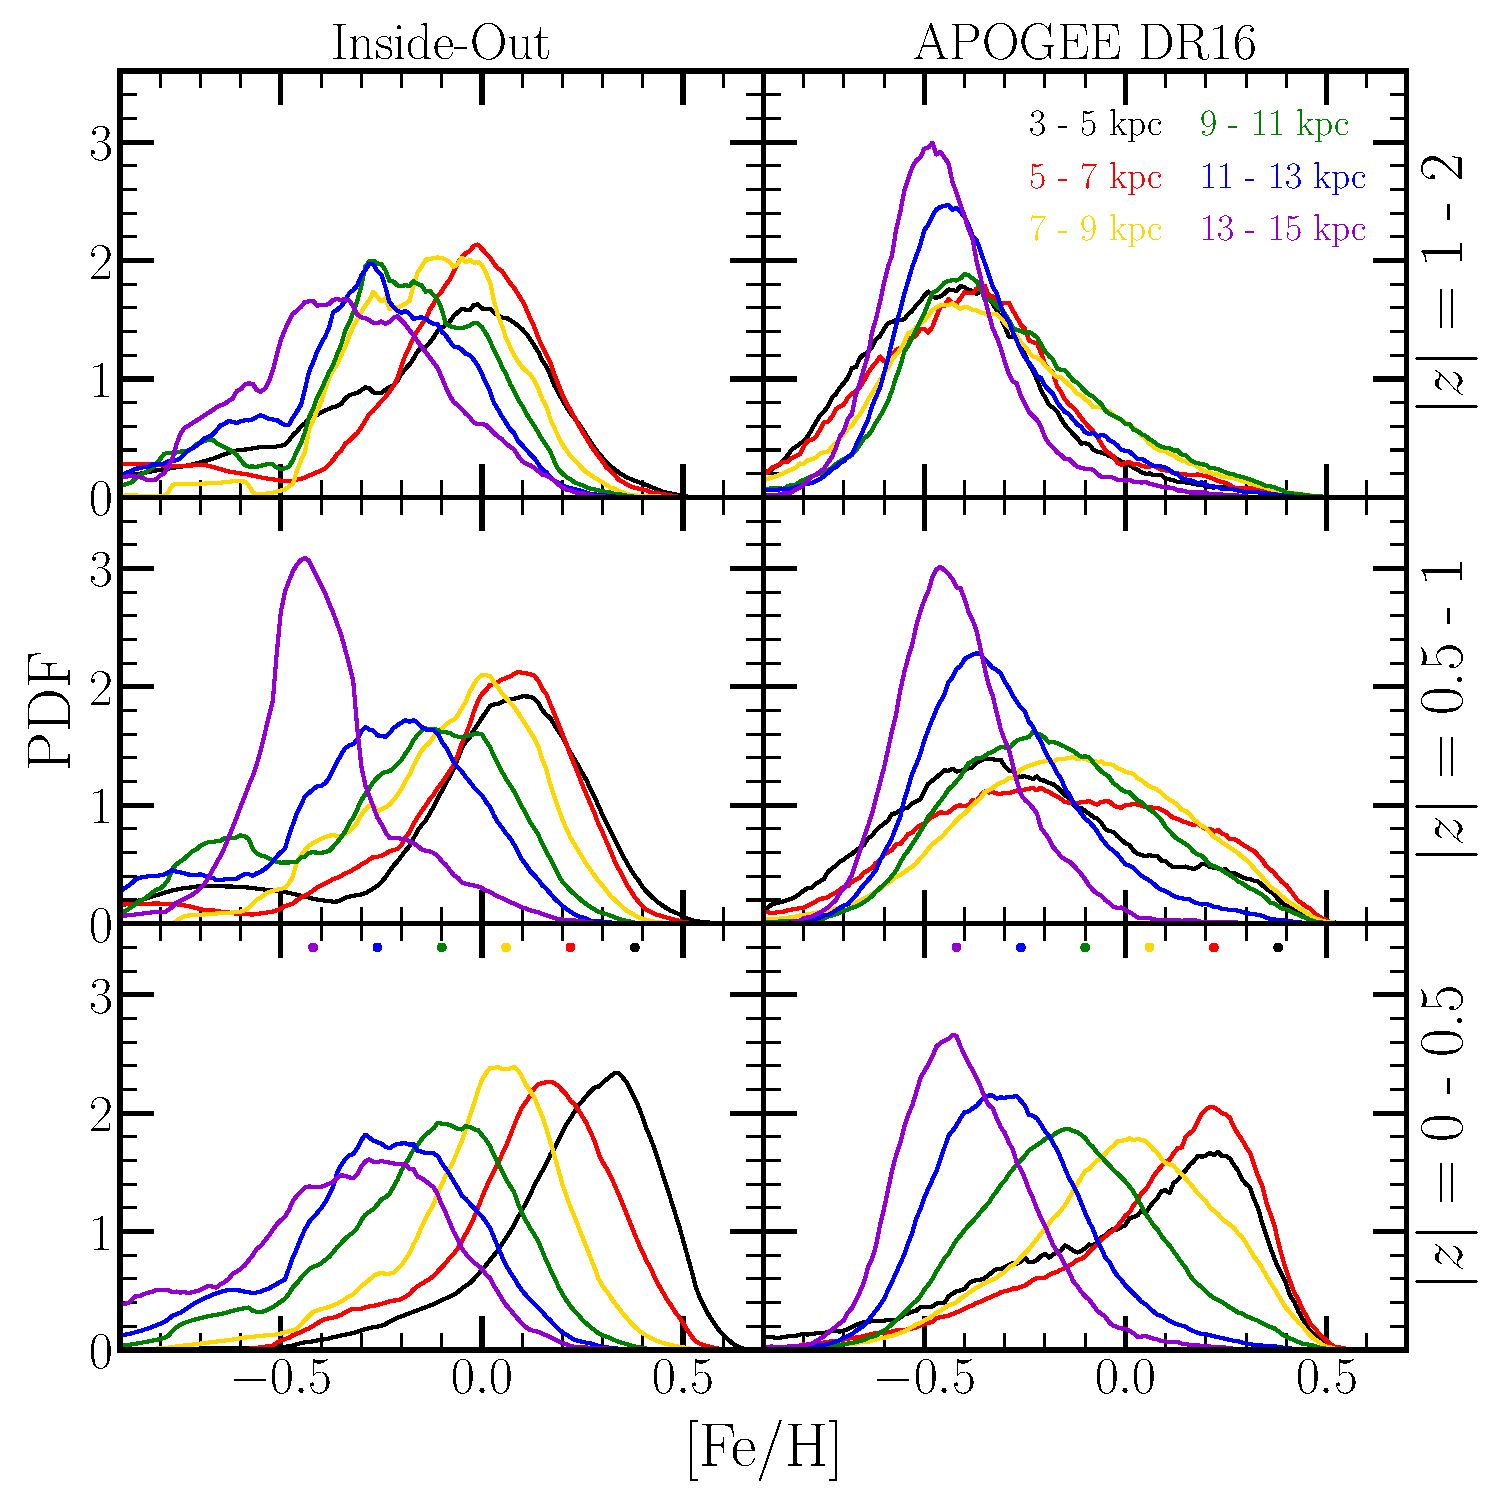
\includegraphics[scale = 0.45]{mdf_3panel_fe.pdf} 
\caption{Metallicity distribution functions (MDFs) in [Fe/H] predicted by our 
fiducial, inside-out model (left) and as observed in APOGEE DR16 (right), for 
stars and simulated stellar populations with present-day~$\left|z\right|$~= 0 - 
0.5 kpc (bottom), 0.5 - 1 kpc (middle), and 1 - 2 kpc (top). MDFs are shown in 
bins of Galactocentric radius: 3 - 5 kpc (black), 5 - 7 kpc (red), 7 - 9 kpc 
(yellow), 9 - 11 kpc (green), 11 - 13 kpc (blue), and 13 - 15 kpc (purple). 
The points near the top of the bottom panels denote what the mode abundance 
would be if it followed out target gradient of [Fe/H] = +0.3 at~$R_\text{gal}$ 
= 4 kpc with a slope of -0.08 kpc$^{-1}$ exactly, assuming the inner radius of 
each bin (i.e. there is no point plotted for 15 kpc). All distributions are 
smoothed with a box-car width of [Fe/H]~$\pm$~0.1 for clarity. } 
\label{migration:fig:mdf_3panel_fe} 
\end{figure} 

% fig 11 
\begin{figure} 
\centering 
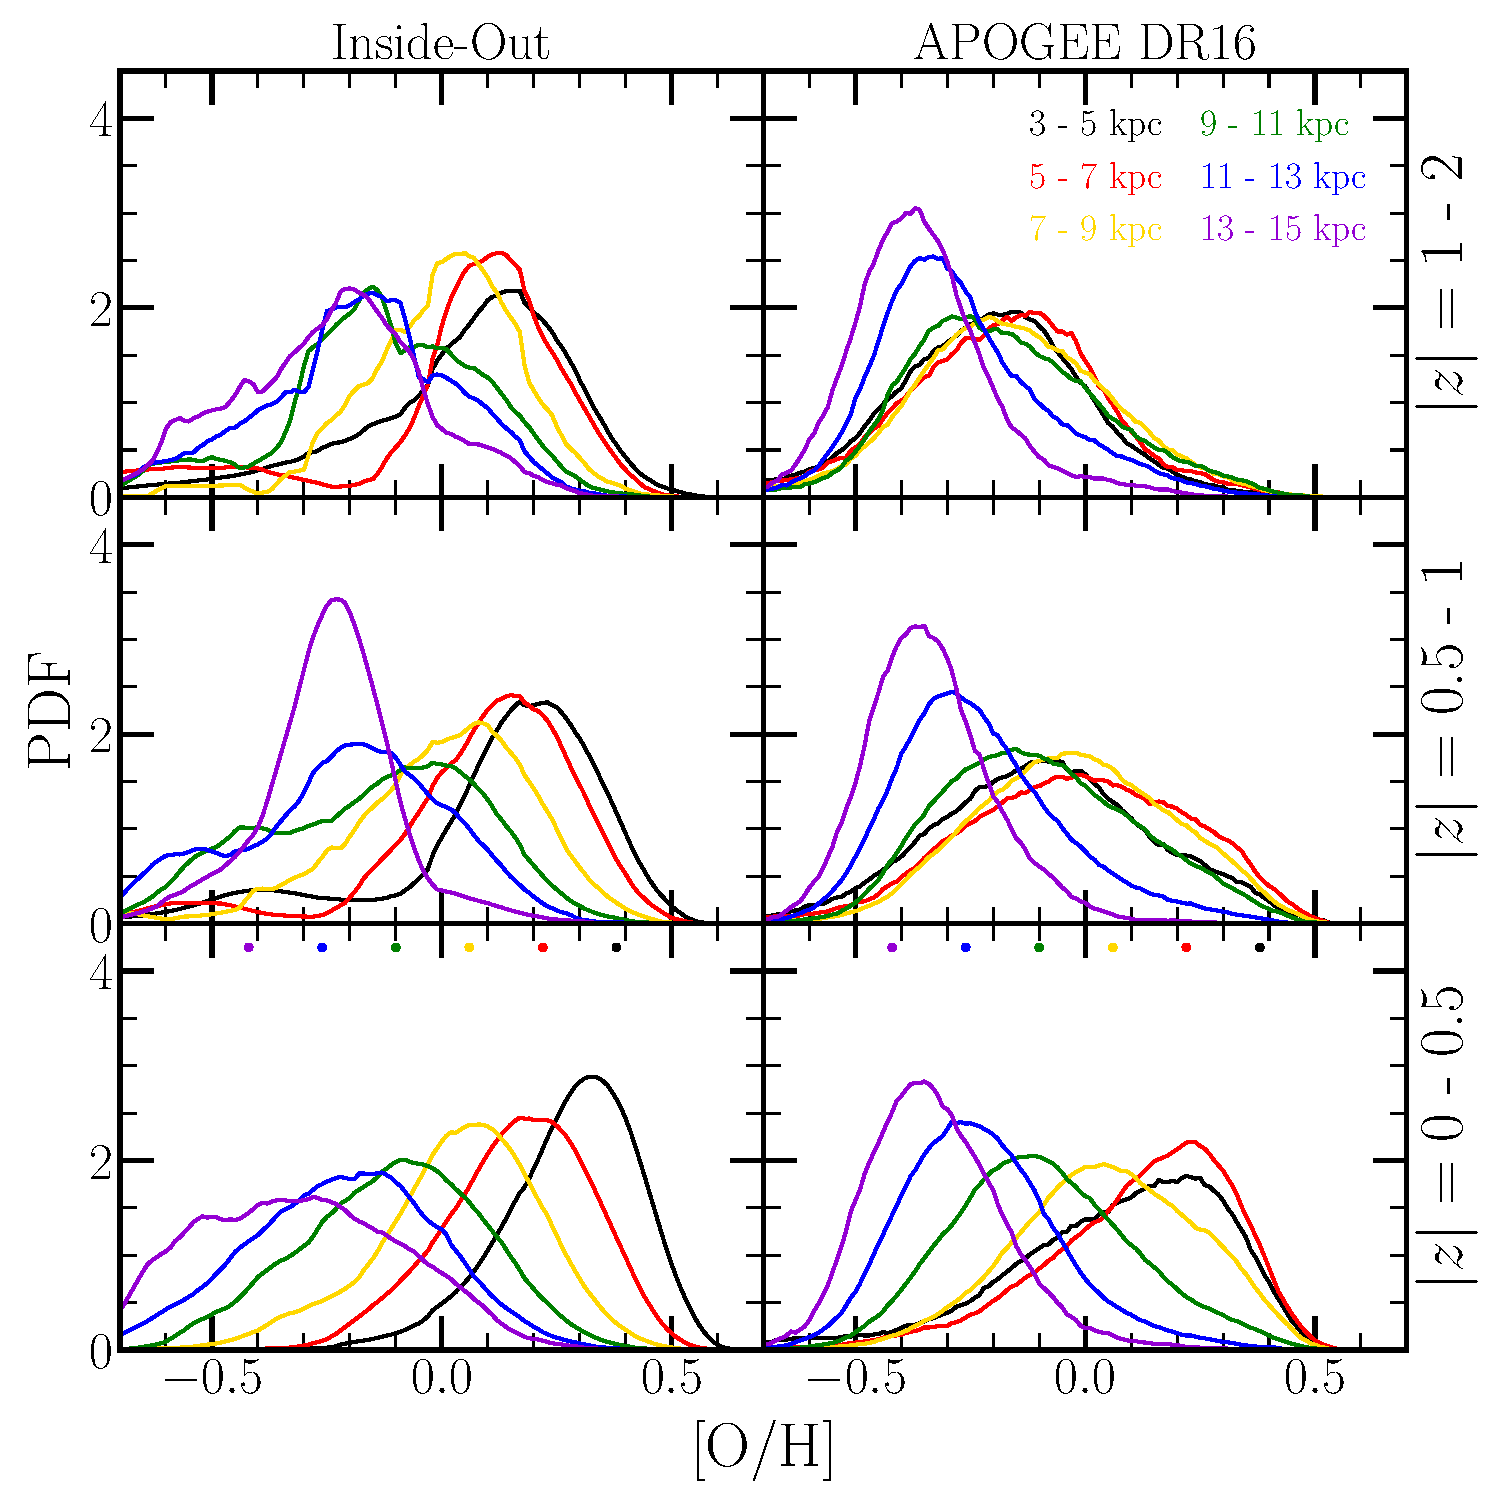
\includegraphics[scale = 0.45]{mdf_3panel_o.pdf} 
\caption{The same as Fig.~\ref{migration:fig:mdf_3panel_fe}, but for [O/H]. } 
\label{migration:fig:mdf_3panel_o} 
\end{figure} 

Metallicity distribution functions (MDFs) and their variations with Galactic 
region are a core prediction of GCE models. 
We have computed distributions of [Fe/H] and [O/H] using abundances from the 
16th data release~\citep[DR16;][]{Ahumada2020, Joensson2020} of APOGEE 
\citep{Majewski2017}. 
Abundances are determined by the APOGEE Stellar Parameters and Chemical 
Abundances Pipeline (ASPCAP;~\citealp{Holtzman2015, GarciaPerez2016}). 
We restrict our sample to stars with effective temperatures of 4000 K 
$\leq T_\text{eff} \leq$~4600 K, surface gravities of 1.0~$\leq \log g \leq$ 
2.5, and signal-to-noise ratios of at least 100. 
These cuts ensure that our sample consists of stars on the upper red giant 
branch, luminous enough to cover all regions of the disc, while excluding red 
clump stars to avoid possible abundance offsets between these stars and stars 
on the giant branch. 
Our observational results are similar to those shown by~\citet{Hayden2015}, 
but we use a larger data set, more recent APOGEE observations, and [O/H] and 
[Fe/H] rather than [$\alpha$/H] and [M/H]. 
\par 
The left and right panels of Fig.~\ref{migration:fig:mdf_3panel_fe} show [Fe/H] 
distributions from our fiducial inside-out model and the APOGEE data, 
respectively, in bins of~\rgal~and~\absz. 
The observed midplane distributions (\absz~$\leq$~0.5 kpc) show the striking 
phenomenon first noted by~\citet{Hayden2015}: a shift from a skew-negative form 
in the inner Galaxy to a skew-positive form in the outer Galaxy, with a roughly 
symmetric [Fe/H] distribution at the solar circle. 
The simulation reproduces this behaviour, confirming that realistic radial 
migration can explain the radial dependence of the MDF shape as conjectured by 
\citet{Hayden2015} and illustrated in a more idealized simulation by 
\citet{Loebman2016}. 
\par 
In detail, the MDFs are not as smooth at large~\rgal~as in the observations; 
they are not as skewed in the inner and outer disc either. 
Dots in the lower left panel mark the target metallicities implied by our 
$\eta(\rgal)$ prescription in equation~\refp{migration:eq:eta_rgal}. 
The modes of the stellar MDFs track these targets quite closely, except at 
\rgal~= 13 - 15 kpc, where the migrated population is so large compared to the 
in-situ population that it reshapes the peak of the MDF as well as the tails. 
The model also predicts a continuing increase of the mode metallicity down to 
\rgal~= 3 - 5 kpc, while the observed mode is the same at 3 - 5 kpc and 5 - 7 
kpc. 
We do not view this as a serious discrepancy, as it could be reduced by a
moderate adjustment of the~$\eta(\rgal)$ recipe so that the metallicity 
gradient in these regions is flat. 
We have computed such a comparison case and find that it does indeed reproduce 
this observational result, though it still underpredicts the skewness at 
small~\rgal. 
% {\color{red} 
It is also possible that the differences at 3 - 5 kpc are due to stars 
associated with the Milky Way's strong bar, which~\citet{Bovy2019} demonstrate 
to be low metallicity (see their Fig. 5). 
With only a weak and transient bar in~\hsim, this is a dynamical effect not 
included in our models (see discussion in~\S~\ref{migration:sec:methods:h277}). 
% It's also possible that the differences at 3 - 5 kpc are due to low metallicity 
% bar stars in the data~\citep[e.g. those observed by][]{Bovy2019}, a dynamical 
% effect not present in~\hsim~(see discussion in~\S~\ref{migration:sec:methods:h277}). 
% }
Alternatively, the flattening of the observed gradient could be a consequence 
of more aggressive quenching of star formation than assumed in our models. 
The surface density of star formation~$\dot{\Sigma}_\star$ in the Milky Way 
is known to reach a maximum at~\rgal~$\approx$ 4 kpc and decline by a factor 
of a few at smaller radii (see Fig. 1 of~\citealp{Peek2009} and Fig. 2 
of~\citealp{Fraternali2012} and data therein). 
Early quenching could cutoff the MDF at high [O/H] and [Fe/H] if it happens 
before the ISM reaches equilibrium abundance. 
Visual inspection of Fig.~\ref{migration:fig:tracks} suggests that this process should 
occur around~$T \approx$ 6 - 8 Gyr if the MDF is to peak at 
[Fe/H]~$\approx$~+0.2 - 0.3. 
\par 
Going up from the midplane, the observed MDFs for the four inner annuli 
(\rgal~< 11 kpc) shift to lower average metallicity, and they converge in 
location and in shape, being roughly symmetric at~\absz~= 0.5 - 1 kpc and 
mildly skew-positive at~\absz~= 1 - 2 kpc. 
Qualitatively, the simulation reproduces this shift of mean metallicity, change 
of shape, and convergence of distributions at different~\rgal, although the 
model does not account for the entirety of the effect. 
We consider this a significant success of this simulation-based approach 
because our GCE model is constructed and tuned in~\rgal~alone, so trends with 
\absz~follow from the combinations of age-metallicity trends, age-velocity 
trends arising from ``upside-down'' disc formation and dynamical heating, and 
correlations between radial migration and vertical energy. 
\citet{Freudenburg2017} showed that chemical evolution in a vertically settling 
gas disc could explain the MDF trend with~\absz~seen by APOGEE in the inner 
disc, and here we see similar behaviour in a more fully ab initio model. 
\citet{Bird2021} showed that the dynamics of the~\hsim~simulation leads to good 
agreement with the observed age-velocity relation, and here we show that 
this success extends qualitatively to the vertical trends of chemical 
abundances. 
\par 
Quantitatively, there are significant differences between the predicted and 
observed distributions above the midplane. 
The model MDFs from~\absz~= 0.5 - 1 kpc are narrower and more skewed than the 
observed MDFs, with higher median [Fe/H]. 
At~\absz~= 1 - 2 kpc, the predicted MDFs are not as strikingly converged as the 
observed MDFs. 
In both the data and the model, the high-\absz~MDFs for the 11 - 13 and 13 - 15 
kpc annuli remain closer to their midplane counterparts. 
The model [O/Fe]-[Fe/H] distributions in the outer Galaxy appear to show the 
imprint of a few large migration episodes (see Fig.~\ref{migration:fig:ofe_feh_diagram}). 
The smoothness of the observed MDFs at these radii and their similarity across 
\absz~suggests a more vigorous stirring. 
\par 
Fig.~\ref{migration:fig:mdf_3panel_o} plots distributions of [O/H] instead of [Fe/H]. 
The appearance is quite similar to Fig.~\ref{migration:fig:mdf_3panel_fe}, which is 
unsurprising but non-trivial given the different timescales of CCSN and SN Ia 
enrichment. 
The agreement and disagreement between the model and data are similar, though 
the discrepancy for~\absz~= 0.5 - 1 kpc is somewhat clearer in [O/H]. 
The model's outer Galaxy MDFs are less irregular in [O/H] than in [Fe/H], an 
indication that some of the structure in the [Fe/H] distributions is caused by 
the large fluctuations in the SN Ia rate as seen in Fig.~\ref{migration:fig:tracks}. 
We have confirmed this conjecture by computing [Fe/H] MDFs for the 
post-processing radial migration prescription, finding that they are indeed 
more smooth at~\rgal~= 11 kpc. 
\par 
The MDF predictions for our other SFH scenarios - constant SFR, late-burst, and 
outer-burst - are different in detail, but they show the same qualitative 
trends as those in Figs.~\ref{migration:fig:mdf_3panel_fe} and~\ref{migration:fig:mdf_3panel_o}. 
Our findings on the radial and vertical trends of the MDF are also similar 
to those of~\citet{Loebman2016}, who use a galaxy simulation evolved from 
rotating gas in a dark matter halo rather than cosmological initial conditions. 
The qualitative similarity of our results across different models implies that 
the radial and vertical trends are a generic effect of radial migration, 
upside-down disc formation, and dynamical heating in a galaxy with realistic 
abundance gradients and time evolution. 


\subsection{[O/Fe] distributions in Bins of [Fe/H]} 
\label{migration:sec:obs_comp:ofe_dists} 

% fig 12 
\afterpage{
\clearpage
\begin{landscape}
\begin{figure*} 
\centering 
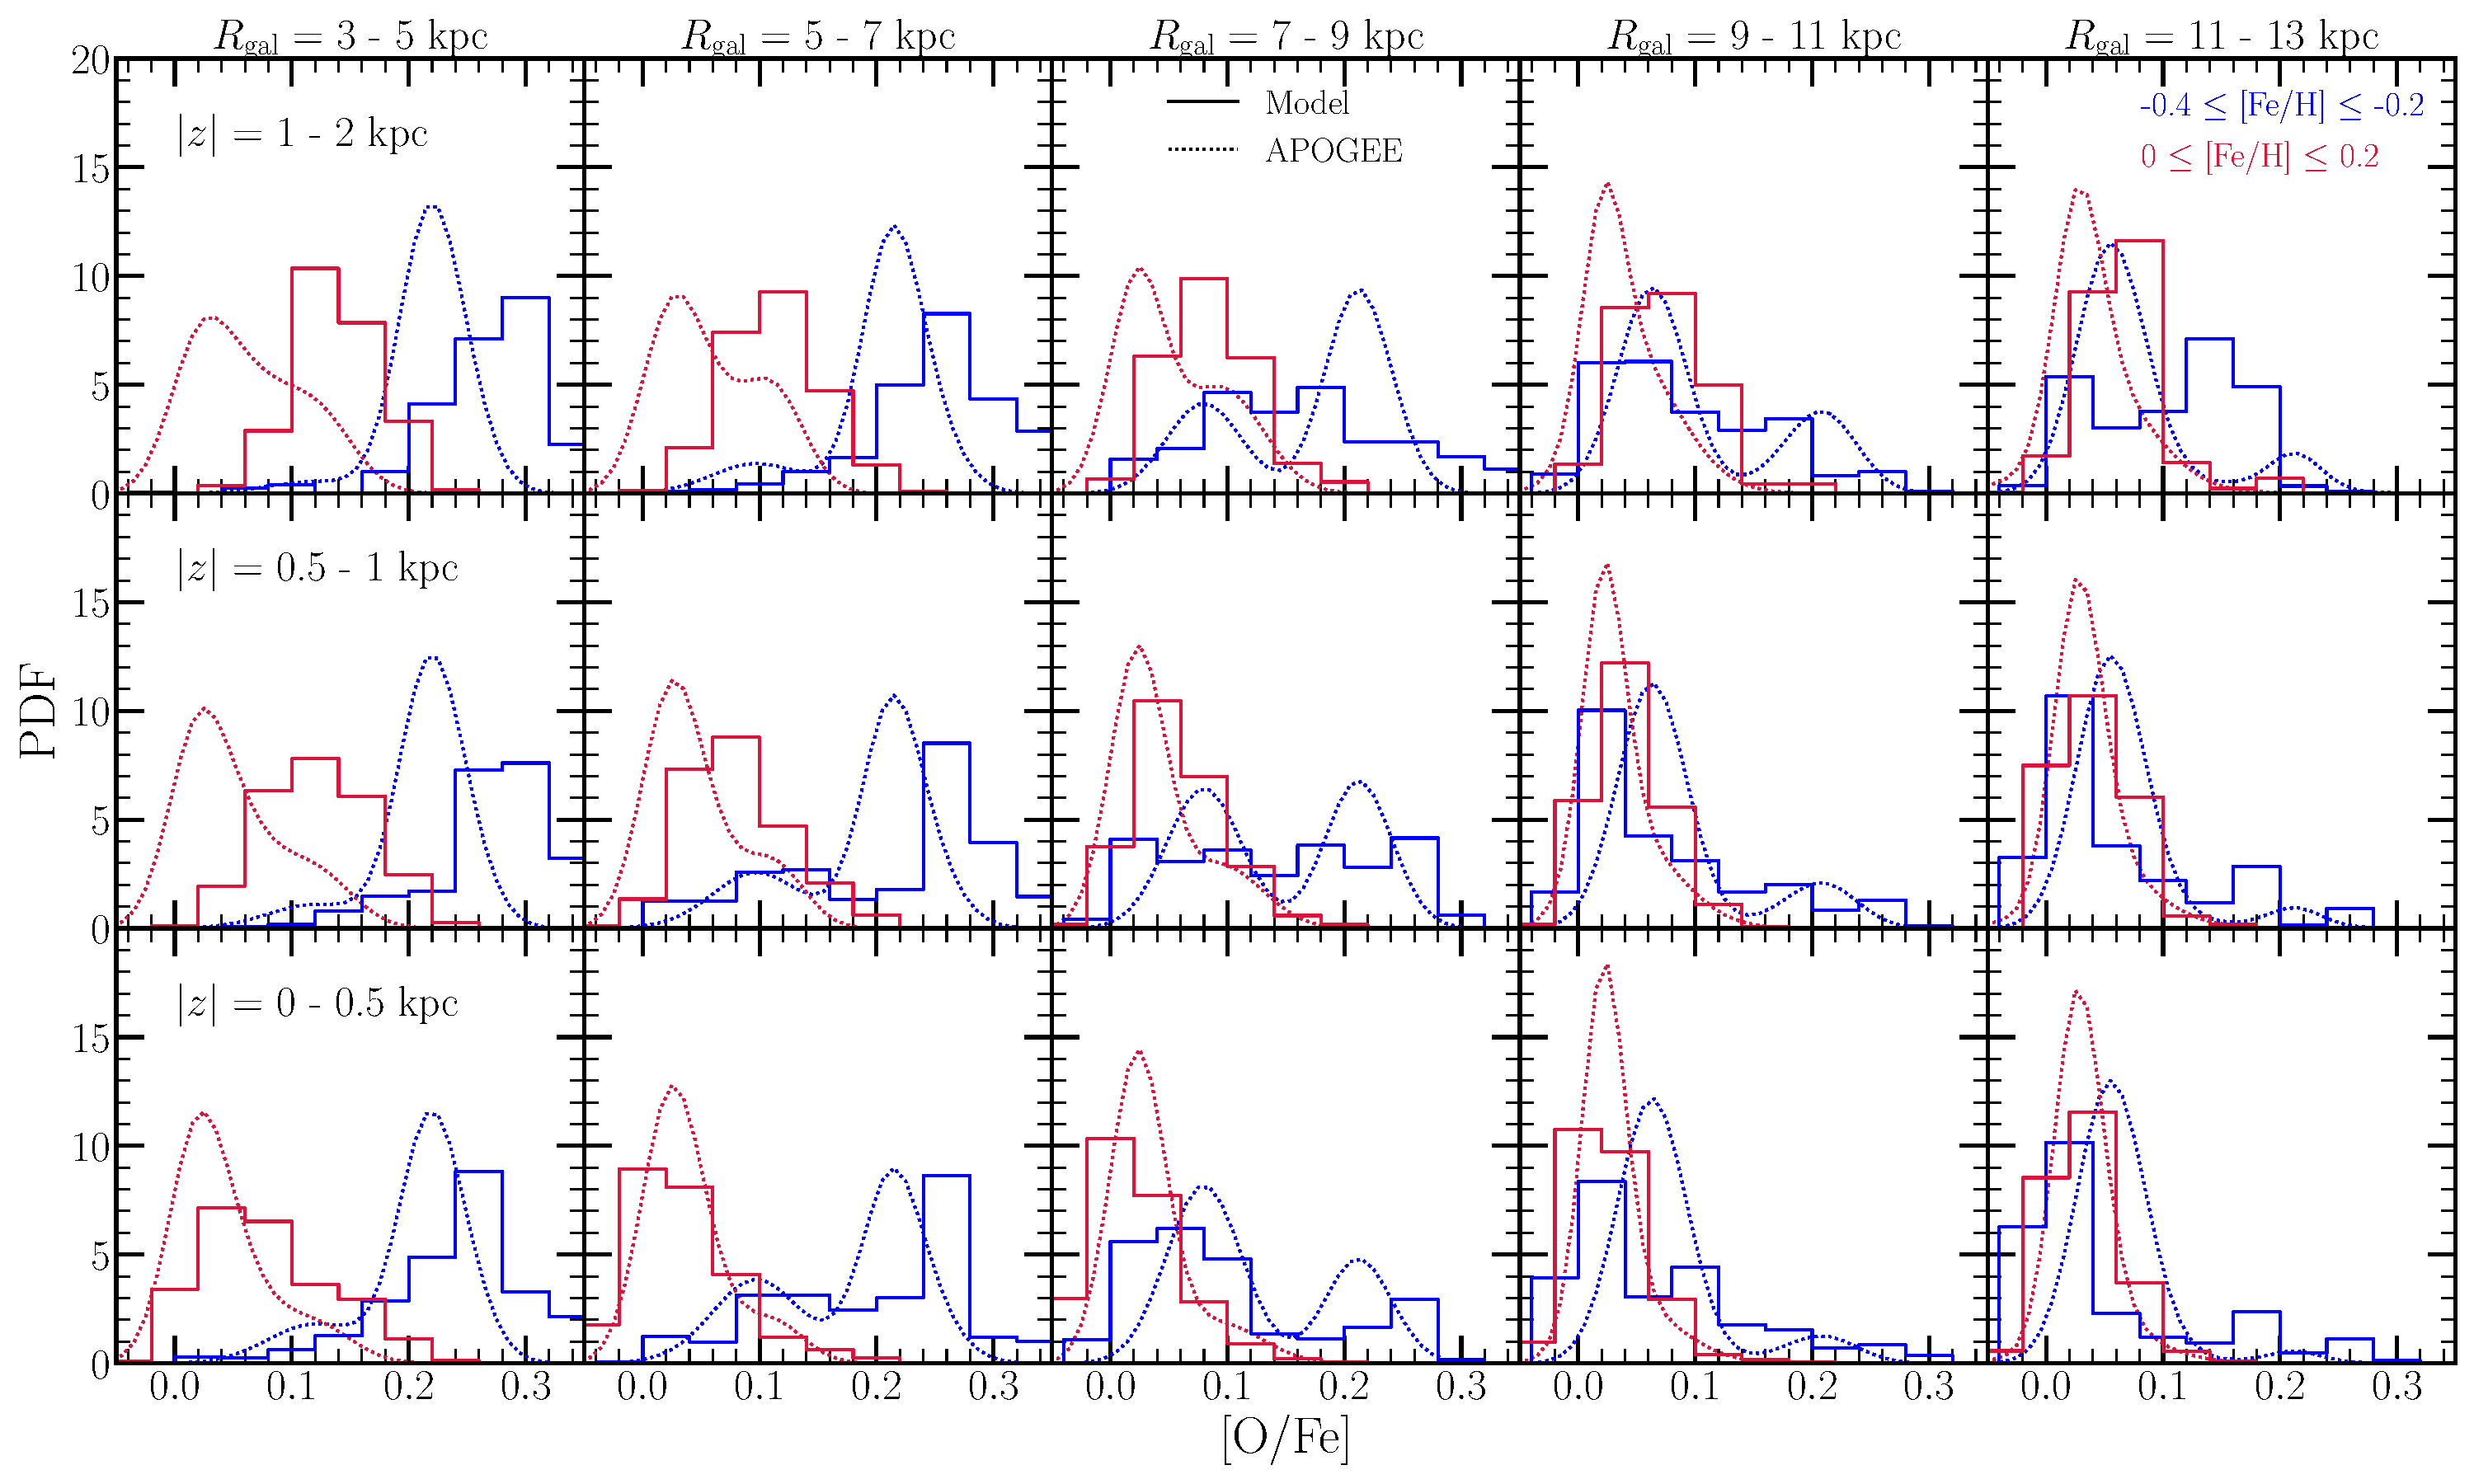
\includegraphics[scale = 0.38]{ofe_mdfs.pdf} 
\caption{Predicted distributions in [O/Fe] in 15 Galactic regions and in two 
bins in [Fe/H]. Columns correspond to bins in~$R_\text{gal}$, denoted at the 
top of each column. Rows correspond to bins in~$\left|z\right|$, denoted in 
text in the left-hand column. Distributions are color-coded according to the 
[Fe/H] the sample is drawn from, denoted by the legend in the upper right 
panel. Solid lines represent that predicted by our inside-out SFH in 
$\Delta$[O/Fe] = 0.04 bins, while dashed lines correspond to the fits to the 
APOGEE DR16 data presented in~\citet{Vincenzo2021a}, which quantify the 
intrinsic distributions accounting for observational uncertainties and the 
APOGEE selection function. } 
\label{migration:fig:ofe_mdfs_insideout} 
\end{figure*} 
\end{landscape}
\clearpage
}

Fig.~\ref{migration:fig:ofe_mdfs_insideout} compares our predicted [O/Fe] distributions 
in Galactic zones to those recently published by 
\citet{Vincenzo2021a}.\footnote{
	\citet{Vincenzo2021a} present [Mg/Fe] distributions in their figures, but 
	they have quantified the [O/Fe] as well, and we use the latter here. 
}
As in our~\S~\ref{migration:sec:obs_comp:mdfs}, they use APOGEE DR16 with similar cuts on 
effective temperature, surface gravity, and signal-to-noise (see their~\S~2). 
They correct for observational scatter as well as age-dependent and (more 
importantly)~\absz-dependent selection in APOGEE to infer the intrinsic 
distribution of [O/Fe] in bins of [Fe/H] that would be found for an unbiased 
sample of long-lived disc stars. 
At a given~\rgal~and [Fe/H],~\citet{Vincenzo2021a} fit a model comprised of two 
Gaussians in [O/Fe], one each for the high-$\alpha$ and low-$\alpha$ 
populations.
The~\absz-dependence of the distribution follows from the empirical scale 
heights of these two populations, taken from~\citet{Bovy2016b}. 
Dotted curves in Fig.~\ref{migration:fig:ofe_mdfs_insideout} show these models integrated 
over the corresponding ranges in~\absz. 
\par 
Solid histograms in Fig.~\ref{migration:fig:ofe_mdfs_insideout} show distributions in 
0.04-dex bins of [O/Fe] for our fiducial inside-out model. 
For clarity we have chosen to focus our comparison on two bins of [Fe/H], one 
just above solar metallicity (0.0~$\leq$ [Fe/H]~$\leq$ 0.2) and one at 
sub-solar metallicity (-0.4~$\leq$ [Fe/H]~$\leq$ -0.2) where the bimodality of 
[O/Fe] is most pronounced. Results for our other models are qualitatively 
similar, and these two [Fe/H] bins illustrate the range of model successes and 
failure. 

% fig 13 
\afterpage{
\clearpage
\begin{landscape}
\begin{figure*} 
\centering 
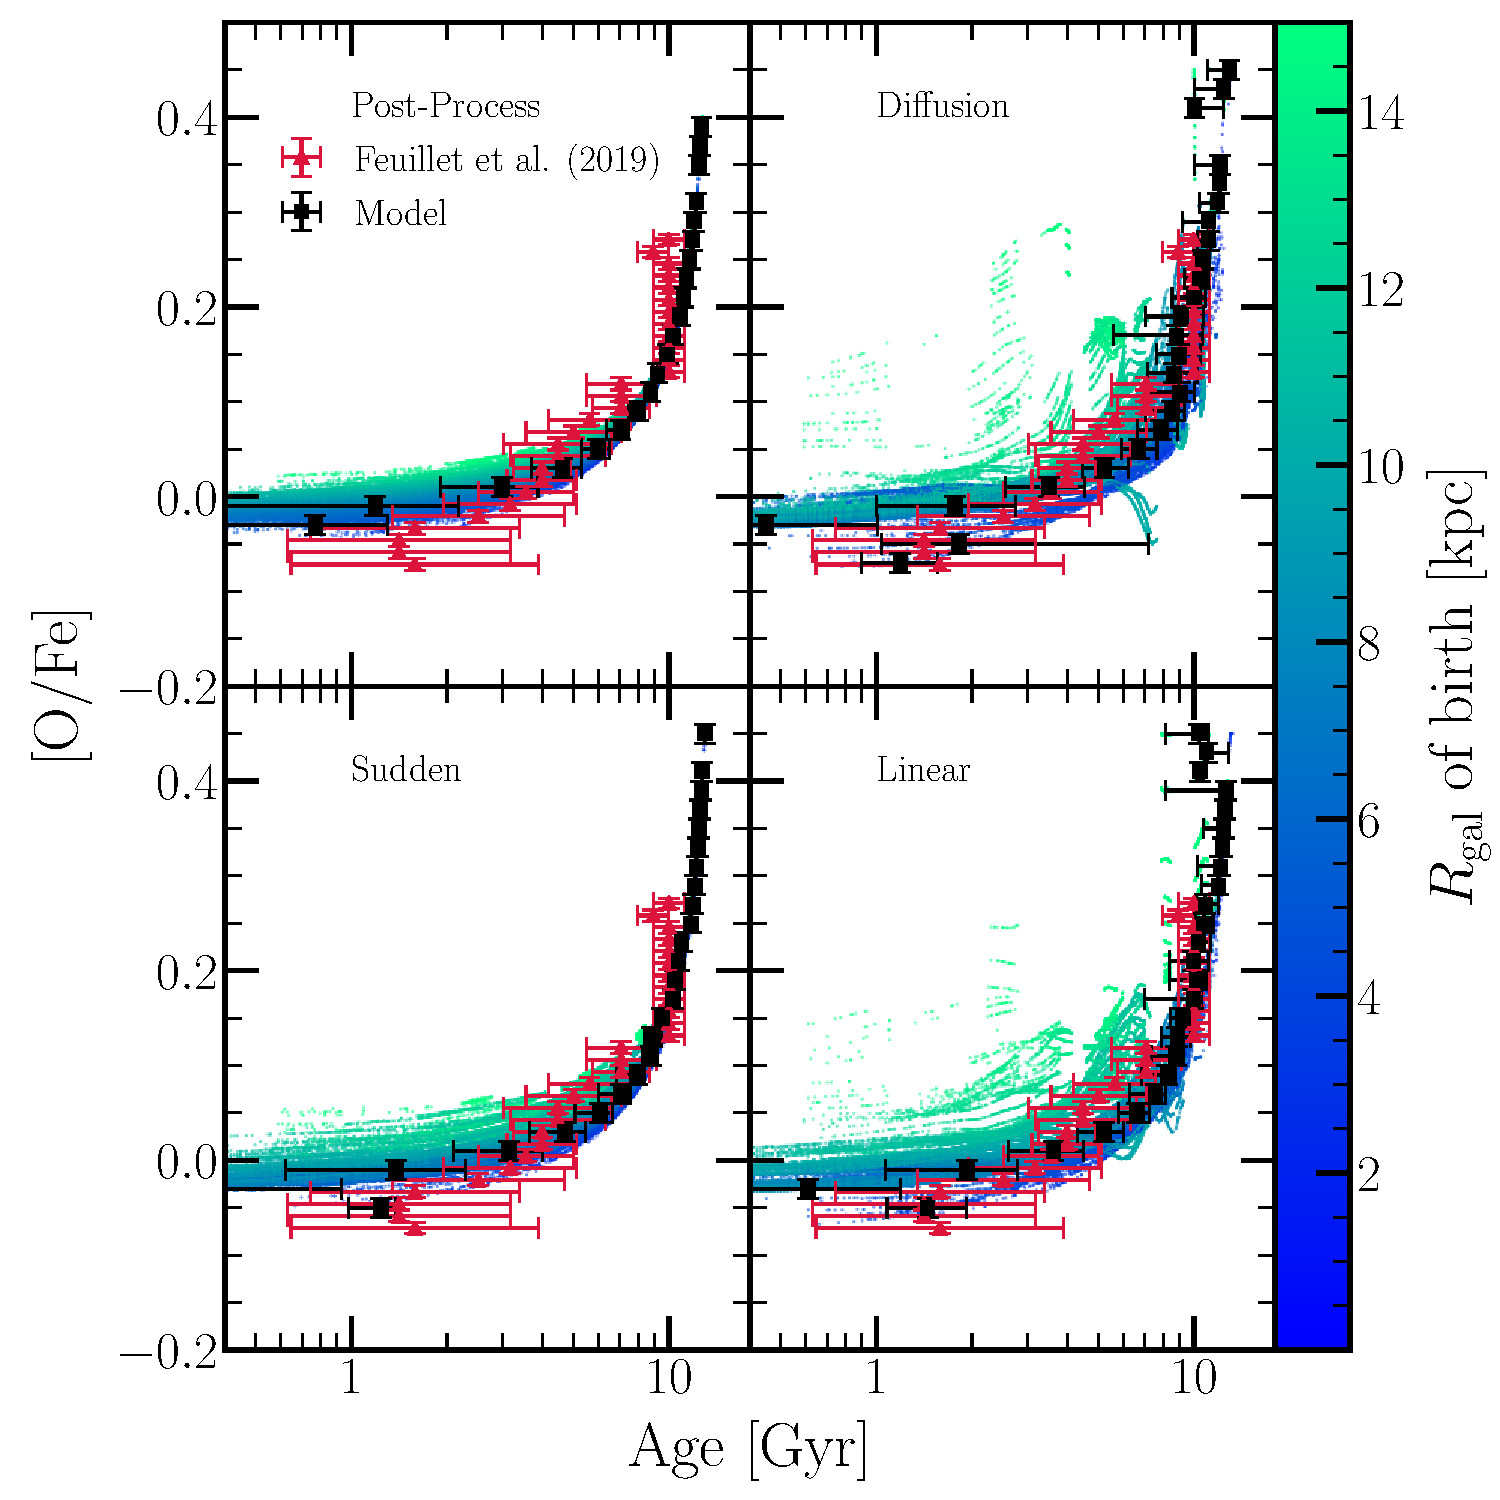
\includegraphics[scale = 0.38]{age_ofe_migration_comparison.pdf} 
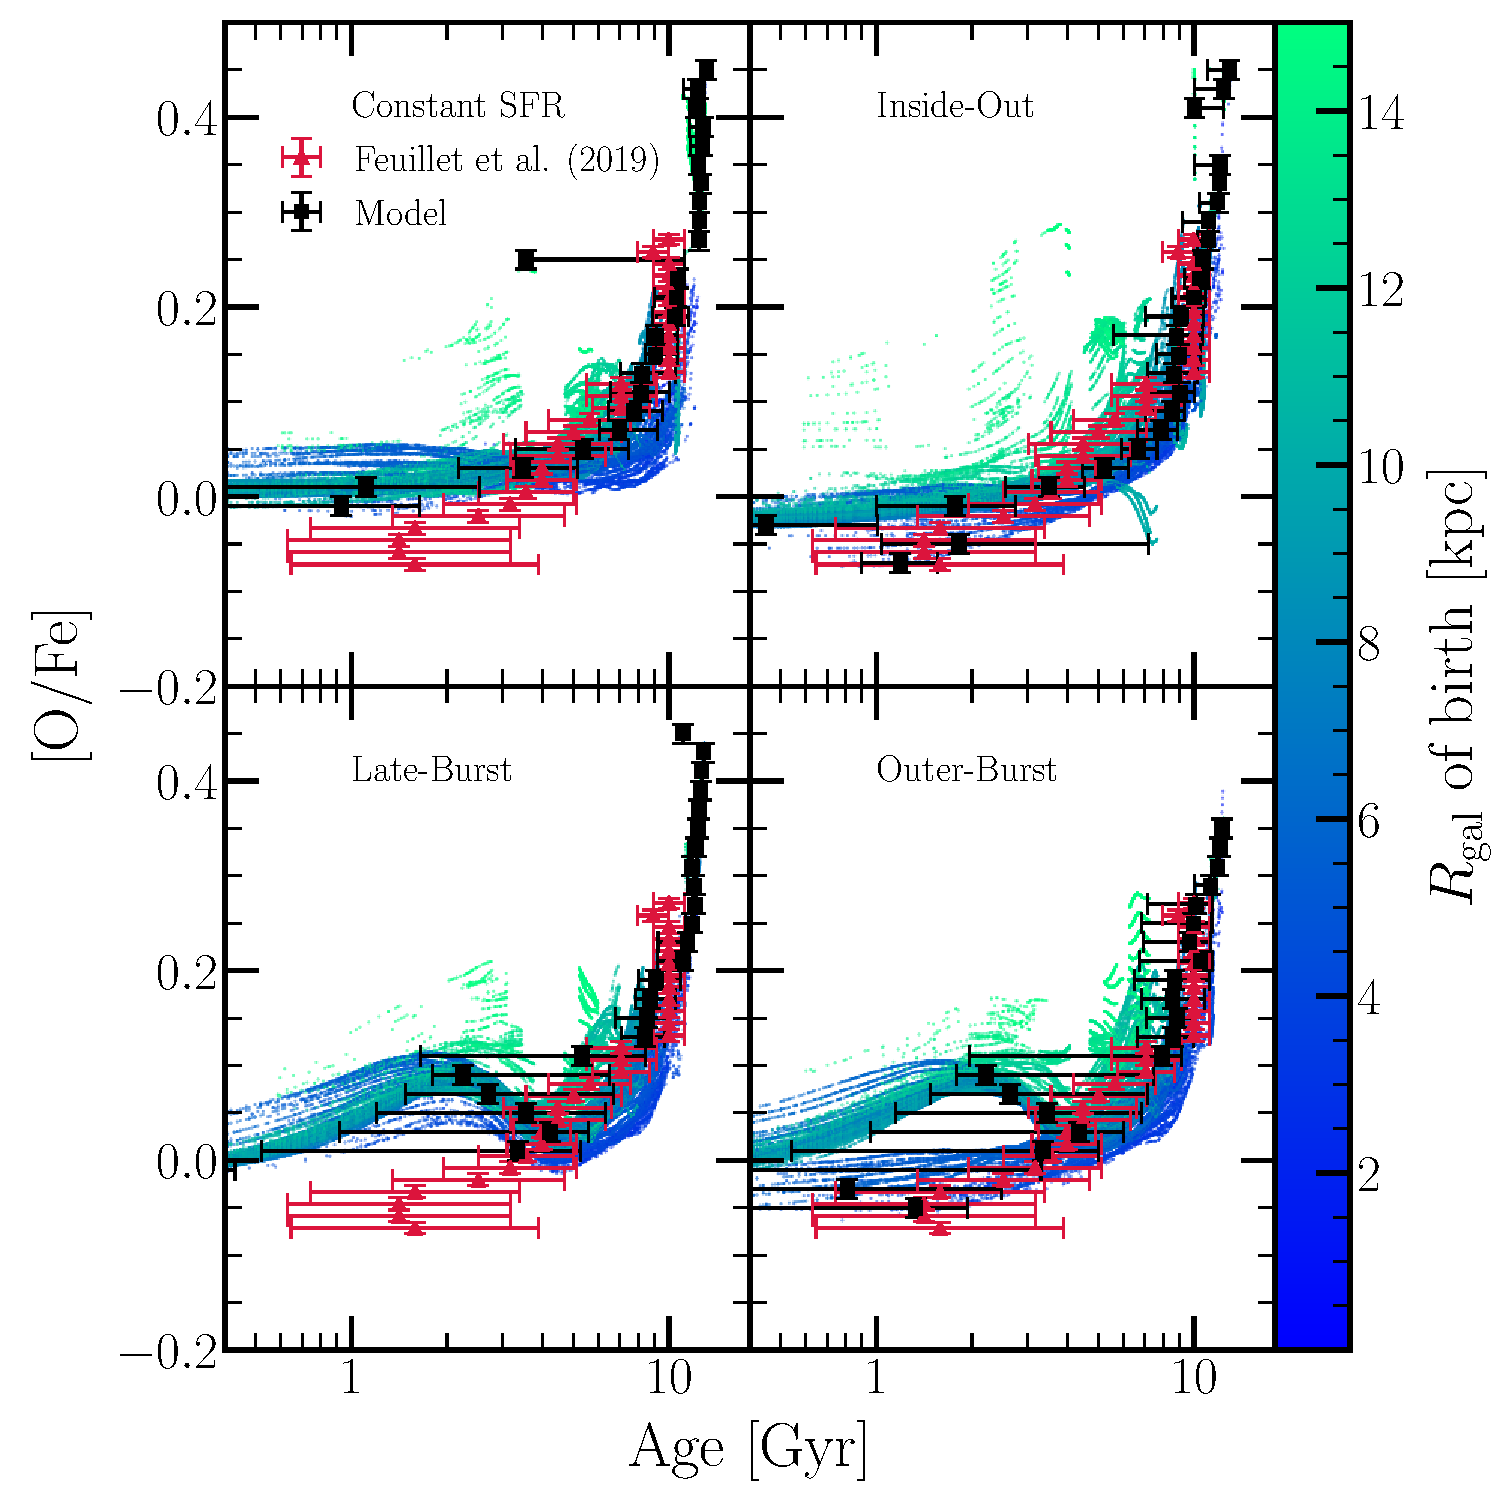
\includegraphics[scale = 0.38]{age_ofe_sfh_comparison.pdf} 
\caption{
\textbf{Left}: A comparison of the predicted age-[O/Fe] relation for the solar 
neighbourhood ($R_\text{gal}$ = 7 - 9 kpc and~$\left|z\right|$ = 0 - 0.5 kpc) 
between the post-processing (upper left), diffusion (upper right), sudden 
(lower left), and linear (lower right) migration models, assuming our 
inside-out SFH. 
\textbf{Right}: The same as the left-hand panels, instead comparing the impact 
of our constant (upper left), inside-out (upper right), late-burst (lower left), 
and outer-burst (lower right) SFHs, assuming diffusion migration. In all panels, 
red triangles and error bars denote the observed median age and dispersion 
thereof in bins of [O/Fe] as reported by~\citet{Feuillet2019}; here we include 
only their bins containing at least 15 stars. Black squares denote the 
mass-weighted median age in 0.02-dex bins in [O/Fe] predicted by our models, 
with error bars denoting the 16th and 84th percentiles of the mass-weighted 
age distribution in those bins. Points in the background denote each individual 
stellar population from the model with a final position in the solar 
neighbourhood, colour-coded according to their Galactocentric radius of birth. 
}
\label{migration:fig:age_alpha} 
\end{figure*} 
\end{landscape}
\clearpage
}

Beginning with the [Fe/H] = 0 - 0.2 bin, we see that the model roughly 
reproduces the observed width of the [O/Fe] distribution. 
In the midplane (\absz~$\leq$ 0.5 kpc) zones it predicts the correct 
skew-positive shape, though the peak of the observed distribution is sharper 
than the model prediction. However, the model histograms shift towards higher 
[O/Fe] with increasing~\absz~while the peak of the observationally inferred 
distributions stays fixed, a discrepancy that is most obvious in the~\rgal~= 
3 - 5 kpc and 5 - 7 kpc bins. The constancy of the observed peak is partly 
a consequence of the~\citet{Vincenzo2021a} fitting procedure, which assumes 
that the location of the high-$\alpha$ and low-$\alpha$ Gaussians stay 
constant at a given~\rgal~and [Fe/H] and only their relative amplitudes change 
with~\absz. We have gone back to the raw data histograms fit by 
\citet{Vincenzo2021a}, and while they do allow some increase in model [O/Fe] 
with~\absz, they do not allow a shift as large as that predicted by our model. 
At~\absz~= 1 - 2 and~\rgal~= 3 - 5 and 5 - 7 kpc, the number of stars 
contributing to the fit is 31 and 17 respectively, so while the shape of the 
distribution is not well constrained, the centroid is robustly determined. 
\par 
This discrepancy could reflect differences in the dynamical heating history 
of the~\hsim~simulation and the Milky Way. 
With its most recent major merger occurring at~$z \approx$ 3, this galaxy was 
previously selected for investigation because of its quiescent merger history 
\citep[e.g.][]{Zolotov2012}. N-body models for the tidal disruption of the 
Sagittarius dwarf galaxy suggest repeated pericentric passages at 1 - 2 Gyr 
intervals~\citep{Law2010}, which could trigger episodes of infall and star 
formation~\citep[e.g.][]{RuizLara2020}. 
These pericentric passages might also heat low-$\alpha$ disc populations to 
higher~\absz, an effect absent in~\hsim. 
Alternatively, we have investigated the impact of changing our~$\eta(\rgal)$ 
prescription to become constant within~\rgal~= 5 kpc, as discussed previously 
in~\S~\ref{migration:sec:obs_comp:mdfs} in the context of the [Fe/H] gradient. 
This change also dampens the predicted trend of [O/Fe] with~\absz~by bringing 
the inner Galaxy's [O/Fe]-[Fe/H] tracks closer together (see 
Figs.~\ref{migration:fig:ofe_feh_diagram} and~\ref{migration:fig:tracks}). 
We find that this change can account for some but not all of the discrepancy, 
shifting the peak of the distribution down by~$\sim$0.05 dex in the upper left 
panel of Fig.~\ref{migration:fig:ofe_mdfs_insideout}. 
\par 
Turning to the -0.4~$\leq$ [Fe/H]~$\leq$ -0.2 bin, the model shows partial but 
by no means complete success. 
It does reproduce the breadth of the [O/Fe] distribution at this intermediate 
metallicity, and in nearly all~\rgal-\absz~zones it predicts skewness of the 
correct sign. 
At~\rgal~= 3 - 5 kpc, the model predicts mode([O/Fe])~$\approx$ 0.3, while 
the observed mode is at [O/Fe]~$\approx$ 0.22. 
This discrepancy is affected by our choice of CCSN yields, which produces an 
[O/Fe] plateau at +0.45. 
While this value is consistent with some observational data (e.g. the 
\citealp*{Ramirez2013} data set modeled by~\citealp{Andrews2017}), APOGEE 
measurements place the plateau at [O/Fe]~$\approx$ +0.3, so it is not 
surprising that our model overpredicts [O/Fe] at low metallicity. 
Unfortunately, uncertainties in the observed abundance scales and the 
theoretical CCSN elemental yields remain an obstacle to sharp GCE model tests. 
\par 
The most significant discrepancy with data is for~\rgal~= 7 - 9 kpc, where the 
observations show a clearly bimodal [O/Fe] distribution in all three~\absz~ 
ranges but the model predicts bimodality only near the midplane. 
This bimodality is also evident in the raw data histograms prior to model 
fitting and correction for selection effects (see Figs. 10 and 11 of 
\citealp{Vincenzo2021a}). 
The idea that radial migration could give rise to an [$\alpha$/Fe] dichotomy 
was proposed by~\citet{Schoenrich2009a}, who noted that the evolutionary tracks 
at any given~\rgal~would produce most stars at low [O/Fe] and that radial 
mixing of these populations would produce a low-$\alpha$ ``sequence'' that is 
a superposition of these evolutionary endpoints. 
\citet{Nidever2014} explored this superposition scenario in the context of 
APOGEE observations, and~\citet{Sharma2021} have recently implemented a 
detailed parameterized scenario matched to APOGEE. 
Although the superposition effect clearly operates in our model, as shown in 
Fig.~\ref{migration:fig:ofe_feh_diagram}, the model produces too many stars at 
intermediate [O/Fe], so there is no clear minimum between the high-$\alpha$ 
and low-$\alpha$ peaks. 
As argued by~\citet{Vincenzo2021a}, the generic problem is that one-zone models 
with smooth evolutionary histories always produce most stars near the low 
[$\alpha$/Fe] endpoints and a much smaller peak at the high-$\alpha$ 
plateau, so one cannot superpose such models in a way that produces strong 
bimodality. 
The~\citet{Sharma2021} model seems like a possible counter-example, but they 
adopt parameterized evolutionary tracks and do not demonstrate that these can 
be drawn from a self-consistent chemical evolution model. 
\par 
The simplest way to produce stronger [$\alpha$/Fe] bimodality in our models 
would be to adopt a two-phase star formation model like that envisioned in 
two-infall scenarios of chemical evolution~\citep[e.g.][]{Chiappini1997, 
Chiappini2001, Romano2010, Grisoni2017, Noguchi2018, Palla2020, Spitoni2016, 
Spitoni2018, Spitoni2019, Spitoni2020, Spitoni2021}. 
% {\color{red} 
\citet{Mackereth2018} find similar conclusions in a sample of 133 Milky 
Way-like galaxies from the EAGLE simulation.
% } 
These scenarios turn down the SFR while the ISM abundances pass through the 
intermediate [$\alpha$/Fe] regime. 
Other scenarios such as large early starbursts~\citep{Clarke2019} or reverse 
[Fe/H] evolution with late-time outflows~\citep{Weinberg2017b} could also 
enhance bimodality, but the late starbursts considered here are insufficient 
on their own. 
We will explore these alternative scenarios for the origin of bimodality in 
future work. 

\subsection{The Age-[$\alpha$/Fe] Relation} 
\label{migration:sec:obs_comp:age_alpha} 

% fig 14 
\afterpage{
\clearpage
\begin{landscape}
\begin{figure*} 
\centering 
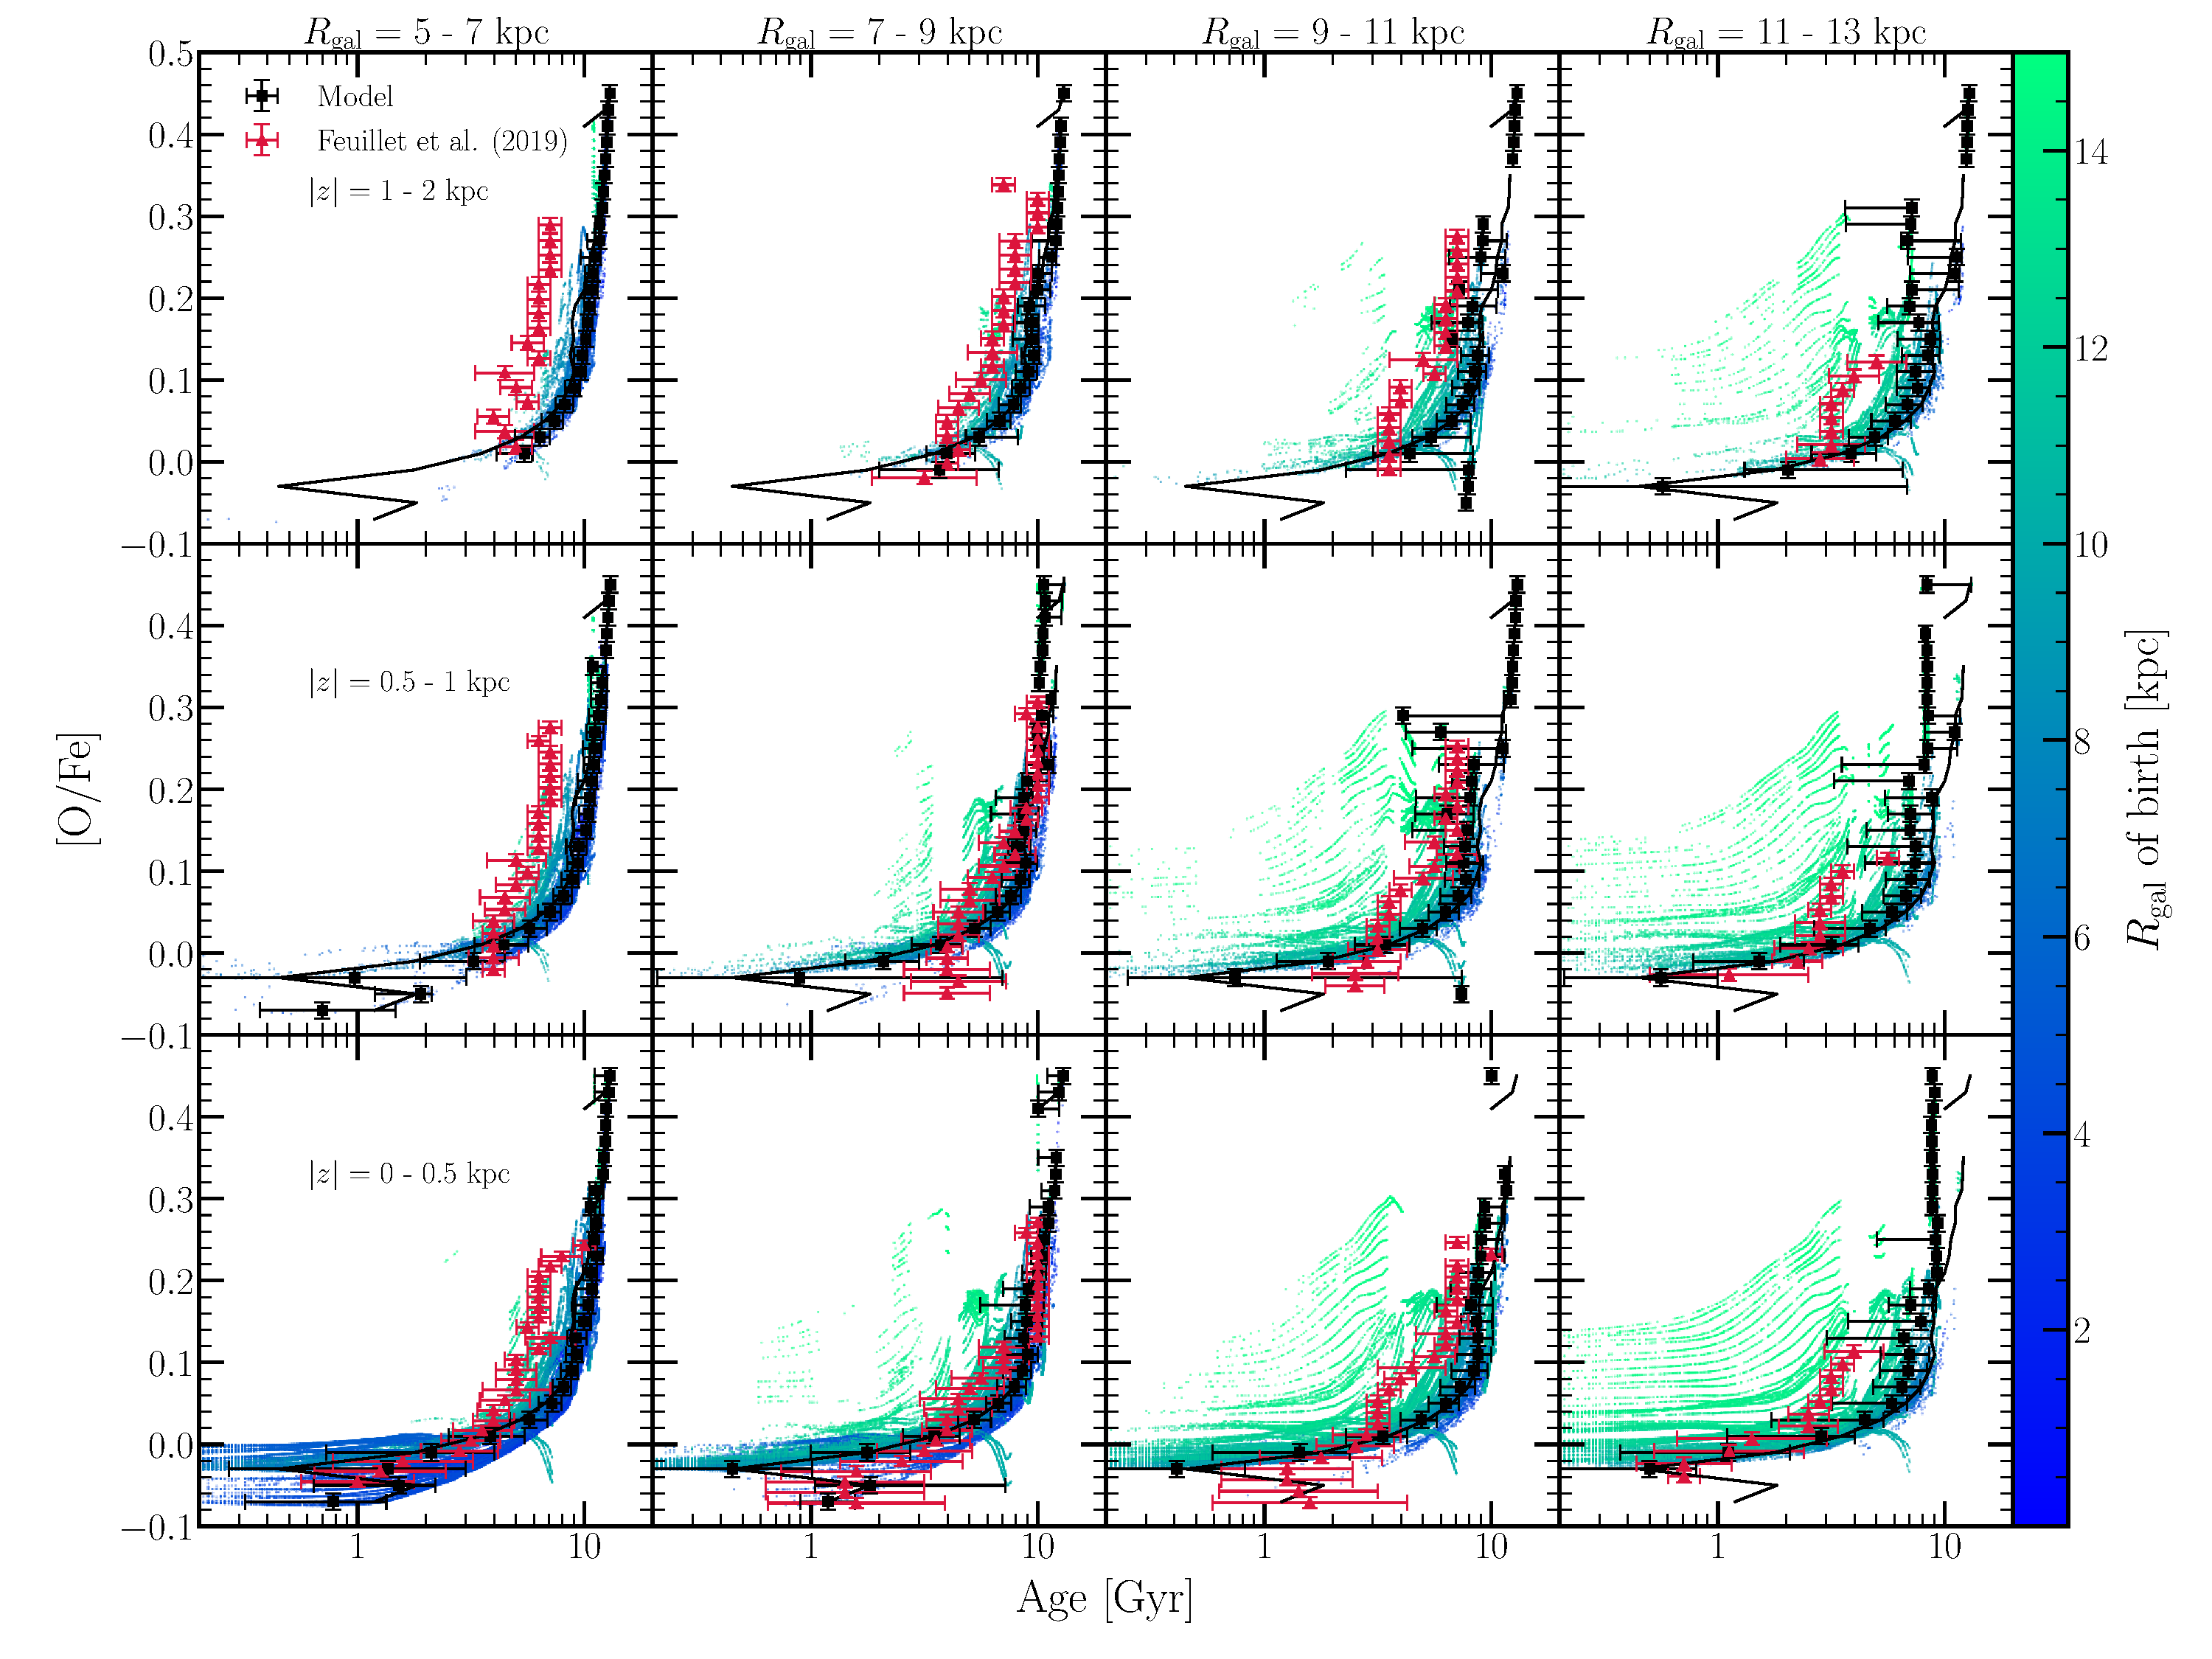
\includegraphics[scale = 0.35]{age_alpha_regions.pdf} 
\caption{The age-[O/Fe] relation in 12 Galactic regions predicted by our 
inside-out SFH. Bins in Galactocentric radius are shown in columns, and labeled 
at the top. 
Bins in the disc midplane distance~\absz~are shown in rows, noted in the 
left-hand column. Red triangles, black squares, 
error bars, and background points are as in Fig.~\ref{migration:fig:age_alpha} for the 
corresponding Galactic region. The solid black line connects the black squares 
in the bottom, left-middle panel, and is replicated elsewhere for reference. } 
\label{migration:fig:age_alpha_regions} 
\end{figure*} 
\end{landscape}
\clearpage
}

In this section, we assess the predicted age-[O/Fe] relations of our models, 
using the results of~\citet{Feuillet2019} as the observational benchmark. 
Their stellar age measurements are based on isochrone matching, 
using APOGEE DR14 stars for which parallax measurements are available 
from~\gaia~\citep{Abolfathi2018, GaiaCollaboration2018}.
With their spatial and quality cuts, the final sample consisted of 77,562 
stars. 
In bins of [O/Fe], they assume a Gaussian distribution of log age, fitting the 
mean (or equivalently, the median) and standard deviation to the stars in that 
bin. 
The choice of a Gaussian distribution is driven by simplicity, enabling 
estimates of mean and spread for data with significant age errors, but because 
our model predicts non-Gaussian log age distributions at fixed [O/Fe], the 
comparison to data is not free of nuance. 
We base most of our model comparisons below on the mass-weighted median age, 
simply denoting the 50th percentile of the mass-weighted age distribution of 
some subsample. 
\par 
In the left-hand set of panels of Fig.~\ref{migration:fig:age_alpha}, we compare the 
age-[O/Fe] relation in the solar neighbourhood ($R_\text{gal}$~= 7 - 9 kpc and 
$\left|z\right|\leq$~0.5 kpc)\footnote{
	In order to avoid confusion, we distinguish between solar ``annulus'' and 
	solar ``neighbourhood'' by defining the solar neighbourhood to be the 
	solar annulus population at~\absz~$\leq$~0.5 kpc. This definition should 
	approximate a sample within a spherical radius of~$\sim$0.5 kpc around the 
	Sun, similar to typical observational definitions. 
} predicted by our four migration models to the 
\citet{Feuillet2019} measurements, shown in red triangles. 
We mark the mass-weighted median age in bins of [O/Fe] in each model with black 
squares, and plot for reference in the background each individual stellar 
population in the solar neighbourhood, colour-coded according to its 
Galactocentric radius of birth. 
\par 
The median age-[O/Fe] trend is similar for all four migration prescriptions, 
and the model prediction is in reasonable agreement with the APOGEE 
measurements. 
From the colour-coding in the post-processing model, one can see that the 
predicted relation is insensitive to the chemical evolution parameters across 
the range represented in our Galactic radial zones, differing only in the 
precise value of [O/Fe] reached at late times. 
Nonetheless, these differences are large enough that radial mixing causes a 
large spread in age at low values of [O/Fe], where the median trend itself 
becomes shallow. 
Nearly all high [O/Fe] stars are old. 
The spread is similar, but not identical, among the four migration 
prescriptions, and it is in reasonable agreement with the observationally 
inferred spread. 
This agreement is a significant success of the migration predicted by the
\hsim~simulation in concert with our GCE model. 
% The observed [O/Fe] distribution extends to values below -0.05 that are not 
% present in our model. This difference could reflect missing stochasticity in 
% our model, or slightly incorrect yield or SFH choices, or observational errors 
% in some [O/Fe] measurements. 
\par 
Although their median trends and characteristic spreads are similar, the 
diffusion and linear migration models show a marked diffrence from the 
post-processing and sudden models, predicting populations of young 
($\lesssim$ 4 Gyr) and intermediate age (4 - 7 Gyr)~$\alpha$-enhanced stars 
([O/Fe]~$\approx$ +0.1 - 0.2) in the solar neighbourhood, which formed at large 
\rgal~with [O/Fe] values well above the main trend for their age. 
They arise from the large fluctuations in the SN Ia rate at large~\rgal~shown 
in Fig.~\ref{migration:fig:tracks} and discussed in~\S~\ref{migration:sec:obs_comp:gradient}, 
which occur when stellar populations migrate to different radii before 
producing most of their SNe Ia. 
% When the SN Ia Fe production rate fluctuates downward, [O/Fe] fluctuates 
% upward in the ISM, and the stars that form from it inherit such a composition. 
% These stars then migrate to the solar annulus. 
% These stars can then migrate to the solar annulus. 
% {\color{red} 
SNe Ia account for~$\sim$60\% of the Fe production at all metallicities 
in our models (see discussion in~\S~\ref{migration:sec:methods:yields}). 
Visual inspection of Fig.~\ref{migration:fig:tracks} indicates that the SN Ia rate can 
vary by as much as a factor of~$\sim$3 at~$\rgal\gtrsim$~9 kpc in our models, 
sometimes more in extreme cases, simply because their progenitors are 
migrating; this corresponds to variability as large as~$\sim$40\% in the total 
Fe enrichment rate if everything else is constant. 
This variability can arise in part out of efficient radial migration moving 
stars away from their birth radii faster than the SN Ia timescale as well as 
the combination of the long tail of the SN Ia DTD and migration on longer 
timescales (see discussion at the end of~\S~\ref{migration:sec:methods:h277}). 
The [$\alpha$/Fe] ratio at a given time is approximately determined by the 
ratio of core collapse to type Ia supernova events occurring over the previous 
depletion time~\citep{Weinberg2017b}, which can be short in the outer Galaxy in 
our models due to the substantial outflows at these radii (see discussion 
in~\S~\ref{migration:sec:methods:outflows}). 
Consequently, when the SN Ia Fe production rate fluctuates downward, [O/Fe] 
fluctuates upward in the ISM. 
An alternative explanation for young~$\alpha$-rich stars is a burst of 
star formation, when the ISM becomes~$\alpha$-enhanced because the CCSN rate 
increases~\citep{Johnson2020}. 
The explanation suggested here is in some sense the opposite: the ISM 
becomes not necessarily~$\alpha$-rich but Fe-poor because of fewer SNe Ia. 
The stars that form inherit such a composition and can then migrate to 
the solar annulus, and our models predict the variability to be sufficiently 
large to explain the high [$\alpha$/Fe] ratios seen in APOGEE. 
% }
% \par\null\par 
\par
The presence of young and intermediate-age~$\alpha$-enhanced stars in APOGEE 
has been demonstrated using ages based on carbon-to-nitrogen ratios 
\citep{Martig2016} calibrated against the asteroseismic ages of the APOKASC 
catalog~\citep{Pinsonneault2014}, and with the asteroseismic ages directly 
\citep{Martig2015, Jofre2016, Izzard2018, SilvaAguirre2018}. 
% \par 
\citet{SilvaAguirre2018} demonstrate that these stars have kinematics similar 
to the rest of the high-$\alpha$ population, and they suggest that they are 
in fact old stars ``rejuvenated'' by mergers or mass transfer events 
% {\color{red} 
as postulated by~\citet{Jofre2016} and~\citet{Izzard2018}. 
In a sample of four young~$\alpha$-enhanced stars observed with Gemini-GRACES, 
\citet{Yong2016} find that two (possibly three) of them show evidence of a 
debris disc, indicative of previous interactions with a binary companion. 
% } 
In a sample of 51 young,~$\alpha$-rich red giants,~\citet{Hekker2019} 
demonstrate that a portion of these stars have carbon-to-nitrogen ratios 
consistent with mass transfer events, but that others do not, indicating that 
they are either truly young stars or the result of mergers on the main 
sequence. 
% \citet{Weinberg2017b} and~\citet{Johnson2020} proposed that
% young~$\alpha$-rich stars could arise in bursts of star formation that 
% enhance the rate of CCSN enrichment. 
% The explanation suggested here is in some sense the opposite: the 
% stars are not so much~$\alpha$-rich as they are Fe-poor because of the 
% deficit in SNe Ia events. 
% {\color{red} 
Our model does not refute mass transfer as an origin for some massive, 
$\alpha$-rich stars, but it can explain the truly young, intrinsically 
$\alpha$-enhanced stars which appear to make up a portion of the 
young~$\alpha$-rich population separate from those which formed via mass 
transfer~\citep{Yong2016, Hekker2019}. 
% }
In our diffusion model,~$\sim$0.2\% of solar neighbourhood stars with 0.1~$\leq$ 
[O/Fe]~$\leq$ 0.2 have ages below 4 Gyr, but~$\sim$13.9\% have ages below 7 Gyr. 
% {\color{red} 
They have a broad distribution in metallicity spanning from [Fe/H]~$\approx-1$ 
to~$\sim$solar, with multiple peaks indicative of separate sub-populations. 
This large spread qualitatively agrees with the findings 
of~\citet{SilvaAguirre2018} (see their Figs. 8 and 10) and~\citet{Miglio2021} 
(see their Fig. 5). 
A direct comparison to data is not free of nuance, because the 
young~$\alpha$-rich stars which formed via mass transfer may outnumber 
those which are intrinsically young~\citep{Miglio2021}. 
% } 

% fig 15 
\begin{figure} 
\centering 
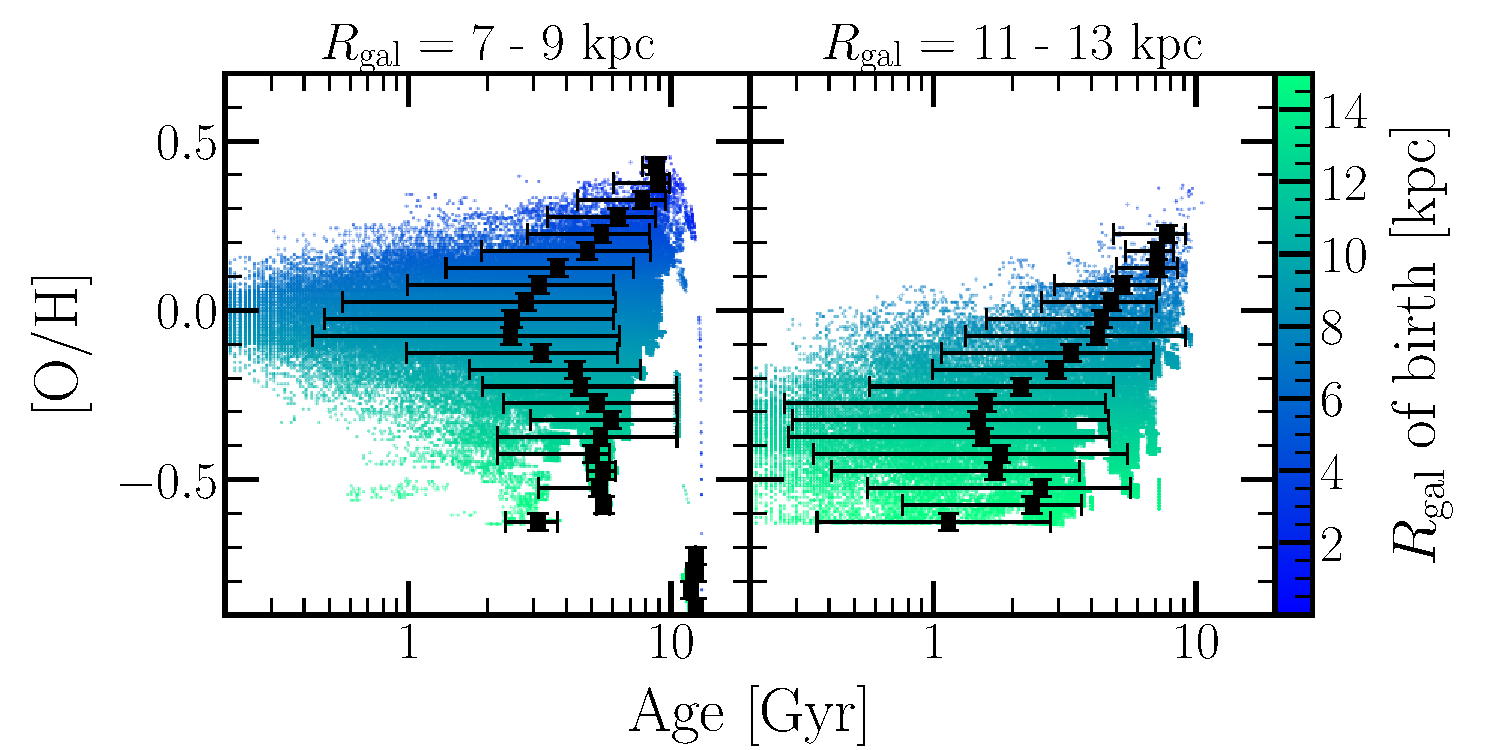
\includegraphics[scale = 0.45]{amr_static_o.pdf} 
\caption{The age-[O/H] relation predicted by our constant SFR model for 
$R_\text{gal}$~= 7 - 9 kpc (left) and 11 - 13 kpc (right). Each panel plots 
only the~$\left|z\right|\leq$~0.5 kpc population. The colored points in the 
background and the black squares with error bars are as in Fig. 
\ref{migration:fig:age_alpha}, but with the model prediction quantified in bins 
of~$\Delta$[O/H] = 0.05. } 
\label{migration:fig:age_oh_static} 
\end{figure} 

The right panels of Fig.~\ref{migration:fig:age_alpha} compare the model predictions of 
our four different SFHs, all assuming the diffusion migration prescription, 
with the same plotting scheme and colour-coding as in the left panels. 
The predicted trend for the constant SFR model is similar to that of the 
inside-out model, but the agreement with data is slightly worse because with a 
constant SFR the evolutionary tracks do not extend below solar [O/Fe]. 
The starburst models, on the other hand, predict a 0.05 - 0.1 dex upward 
fluctuation in [O/Fe] at ages of 1 - 3 Gyr due to the perturbed ratio of 
core-collapse to Type Ia supernova rates~\citep{Johnson2020}. 
In the outer-burst model, stars formed at~\rgal~> 6 kpc follow this perturbed 
track while stars from the inner Galaxy follow the original track. 
These models are motivated by observational results which provide empirical 
evidence for elevated recent star formation~\citep{Mor2019, Isern2019}. 
However, in conjunction with our chemical evolution prescriptions they produce 
clear disagreement with the age-[O/Fe] distributions of~\citet{Feuillet2019} 
and~\citet{Miglio2021}. 
This disagreement could indicate that the starbursts were more limited in 
Galactic radius than we have assumed, or that some other ingredient is missing 
from our models. 
The discrepancy in these panels also implies that if young~$\alpha$-rich stars 
do arise in a starburst, then it must remain sufficiently localized that the 
resultant stellar populations remain outliers from an otherwise monotonic 
age-[$\alpha$/Fe] relation. 
\par 
Fig.~\ref{migration:fig:age_alpha_regions} extends the comparison of our baseline, 
inside-out model and the observations of~\citet{Feuillet2019} to other 
Galactic regions. 
The predicted median age-[O/Fe] trend is nearly independent of location, as we 
can see by comparing the black model points in each panel to the black line, 
which shows the solar neighbourhood prediction. 
~\citet{Feuillet2019} report ages for~$\alpha$-rich stars that are younger at 
large~$R_\text{gal}$ and high $\left|z\right|$, though in most cases only by 
$\sim$20\%. 
Our model predicts a larger population of intermediate-age~$\alpha$-rich stars 
at large~\rgal, but this effect is not large enough to reproduce the observed 
trend. 
None of our model variants reproduce this trend of age-[O/Fe] offset with~\absz, 
so if the observational result is correct then it points to a missing 
ingredient in the model. 
As with the overpredicted [O/Fe] ratios at 
small~\rgal~(\S~\ref{migration:sec:obs_comp:ofe_dists}), dynamical stirring of younger 
disc populations to higher~\absz~by the Sagittarius dwarf could play a role in 
resolving this discrepancy. 
However, Fig.~\ref{migration:fig:age_alpha_regions} shows that the model does not have a 
reservoir of younger high-$\alpha$ stars at low-\absz~available to be stirred, 
so some additional change would likely be needed. 
Furthermore, our model predicts the 16th-84th percentile ranges of the age 
distribution at fixed [O/Fe] to increase for [O/Fe]~$\gtrsim$ +0.1 stars, at 
least in part due to the higher frequency of young and intermediate-age 
$\alpha$-rich stars. 
This increase in the intrinsic scatter of the relation is simply a consequence 
of the SN Ia rate variability having a higher amplitude at large~\rgal~(see 
discussion in~\S~\ref{migration:sec:obs_comp:gradient}). 
\par 
In this paper, Fe is the only element that we consider with a delayed 
nucleosynthetic source. 
Nonetheless, we expect stellar migration to induce similar variability and 
scatter for other elements with delayed sources. 
Elements such as strontium (Sr) are produced by the $s$-process in AGB stars on 
a timescale intermediate between CCSN and SN Ia enrichment (see Fig. 5 of 
\citealp{Johnson2020}), and elements with a large contribution from low mass 
AGB stars could trace longer timescales. 
The DTD for $r$-process elements such as europium (Eu) is uncertain because the 
relative importance of prompt sources (e.g., collapsars) and delayed sources 
(e.g., neutron star mergers) remains poorly constrained~\citep{Cote2019, 
Mishenina2019, Siegel2019, Vincenzo2021b}. 
Using hydrodynamical simulations from the Auriga project~\citep{Grand2017}, 
\citet{vandeVoort2020} indeed find that the intrinsic scatter in $r$-process 
abundances increases for models with longer characteristic delay times. 
Future comparisons of observed trends between age and abundance ratios with the 
predictions of models like those presented here could better isolate missing 
ingredients of the models, as well as potentially improving understanding of 
the nucleosynthetic sources. 
% \par 
% {\color{red} (The next paragraph probably moving to conclusions) I added a 
% couple sentences to the prior paragraph that, with what is currently stated in 
% the conclusions, may make this redundant. -James}  
% In our models, radial mixing of populations with different evolutionary tracks 
% is the only effect that creates a spread of abundance ([Fe/H] and [O/Fe]) at 
% fixed age at a given final~\rgal. 
% The trend of evolutionary tracks with birth radius is fairly smooth, though 
% the impact of migration on SN Ia rates creates stochastic variations that 
% give rise to the young and intermediate-age~$\alpha$-rich stars in our models. 
% Incomplete mixing of the ISM in azimuth and~\absz~\citep{Krumholz2018b} is an 
% additional source of stochasticity in chemical evolution that is currently not 
% represented in our models. 
% This stochasticity will be larger for elements produced by rare events, such as 
% neutron star mergers, and there have been some recent theoretical 
% investigations of predicted scatter in~$r$-process abundances from this source 
% \citep[e.g.][]{vandeVoort2020}. 
% Observationally, the correlation of residual abundances (i.e., of deviations 
% from mean trends) may be a more sensitive probe of stochasticity and mixing 
% than variance of abundance ratios~\citep{Ting2021}. Characterizing the physics 
% of element mixing in the ISM and the stochastic effects on chemical evolution 
% is an important frontier for models and observations. 

\subsection{The Age-Metallicity Relation} 
\label{migration:sec:obs_comp:amr} 

% fig 16 
\begin{figure} 
\centering 
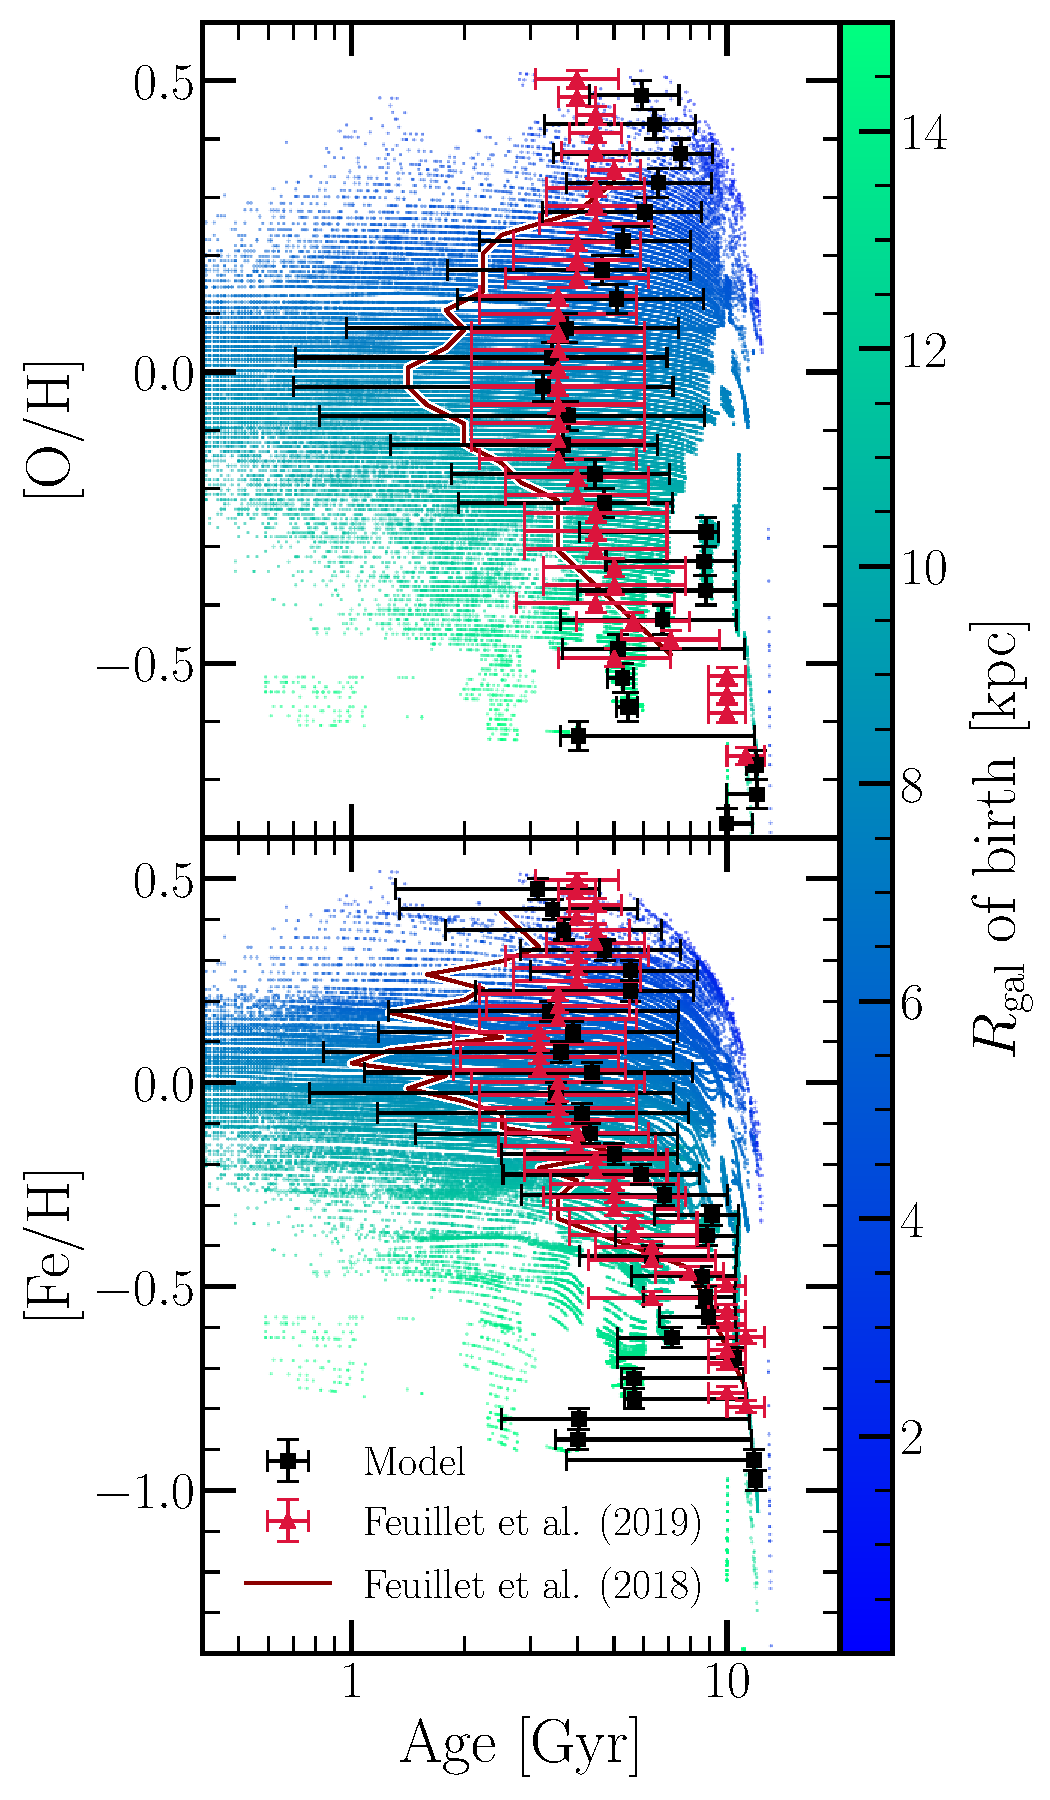
\includegraphics[scale = 0.5]{amr_solar_annulus.pdf} 
\caption{The age-[O/H] (top) and age-[Fe/H] (bottom) relations for the solar 
neighbourhood (i.e.~$R_\text{gal}$ = 7 - 9 kpc,~$\left|z\right|\leq$~0.5 kpc) 
as predicted by the fiducial model. Red triangles, black squares, error bars, 
and background points are as in Fig.~\ref{migration:fig:age_alpha}, but with the model 
prediction quantified in bins of~$\Delta$[O/H] =~$\Delta$[Fe/H] = 0.05. For 
comparison, we plot the~\citet{Feuillet2018} measurements in a dark red line, 
omitting the associated uncertainties for visual clarity. } 
\label{migration:fig:amr_solar_annulus} 
\end{figure} 

% fig 17 
\afterpage{
\clearpage
\begin{landscape}
\begin{figure*} 
\centering 
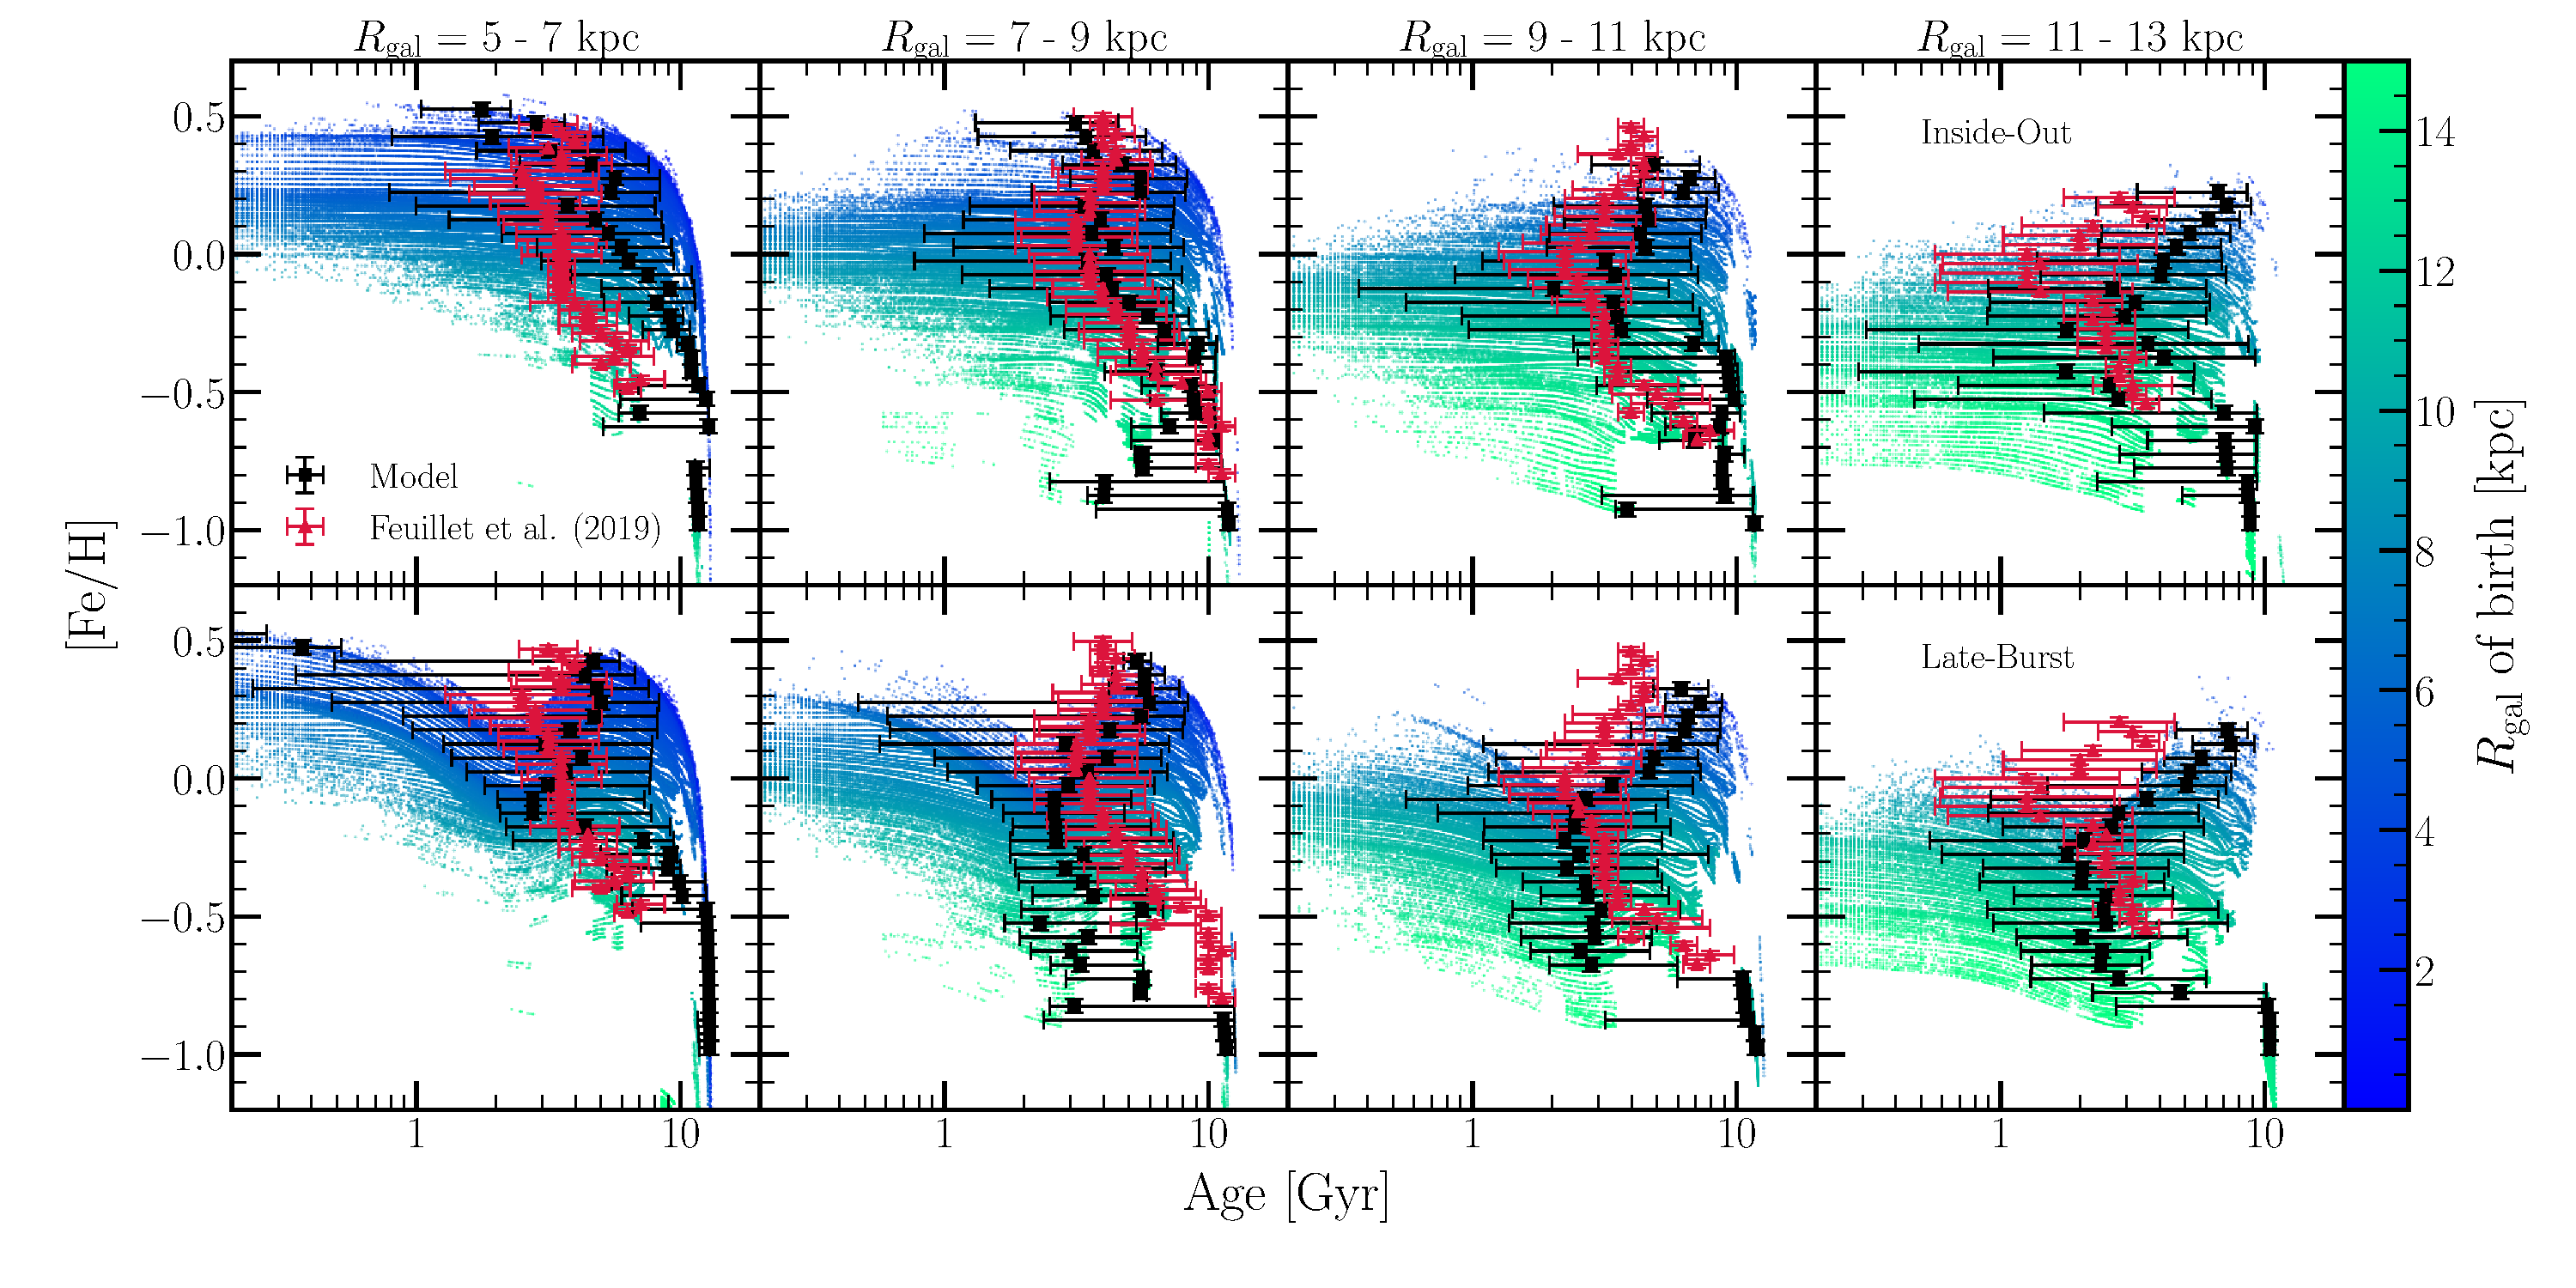
\includegraphics[scale = 0.4]{amr_insideout_vs_lateburst_fe.pdf} 
\caption{The age-[Fe/H] relation predicted by our inside-out (top) and 
late-burst (bottom) SFH models for~$R_\text{gal}$ = 5 - 7 kpc (left), 7 - 9 kpc 
(left middle), 9 - 11 kpc (right middle), and 11 - 13 kpc (right). Each panel 
shows only the~$\left|z\right|\leq$~0.5 kpc population. Red triangles, black 
squares, error bars, and coloured points are as in Fig.~\ref{migration:fig:age_alpha} for 
the corresponding Galactic region, but with the model prediction quantified in 
bins of~$\Delta$[Fe/H] = 0.05. } 
\label{migration:fig:amr_insideout_vs_lateburst_fe} 
\end{figure*} 
\end{landscape}
\clearpage
}

Although the AMR is usually formulated in terms of 
[Fe/H], it is also interesting to quantify the age-[O/H] relation because it 
is not affected by SN Ia enrichment. 
The extent to which the two AMRs differ indicates the extent to which the 
delayed timescale and impact of migration on SN Ia enrichment are important in 
shaping the age-[Fe/H] relation. 
Fig.~\ref{migration:fig:age_oh_static} presents the age-[O/H] relation predicted by our 
constant SFR model for the~$\left|z\right|\leq$~0.5 kpc population at 
$R_\text{gal}$ = 7 - 9 and 11 - 13 kpc. 
The black squares with error bars denote the mass-weighted median age as 
in~\S~\ref{migration:sec:obs_comp:age_alpha}, and we again plot the individual stellar 
populations in the background for reference, colour-coded according to their 
Galactocentric radius of birth. 
We omit the~\citet{Feuillet2019} measurements from this figure but present 
observational comparisons for our more empirically motivated inside-out SFH 
model below. 
The constant SFR model allows us to isolate the effects of stellar migration 
from the time-dependent SFR. 
\par 
The intrinsic scatter in the observed AMR has previously been interpreted as 
evidence for radial mixing~\citep{Edvardsson1993, Sellwood2002}. 
In the solar neighbourhood,~\citet{Feuillet2018} demonstrate that the most 
metal-rich stars tend to be significantly older than solar metallicity stars. 
Using the \citet{Weinberg2017b} analytic models of one-zone chemical evolution 
coupled to a simplified recipe for radial mixing, they argue that this 
non-monotonic trend is the result of old stars born at small~\rgal~where the 
equilibrium abundance is high. 
Only the old stars are able to migrate to the solar neighbourhood due to the 
time required for such a change in their orbital radius. 
\par 
Fig.~\ref{migration:fig:age_oh_static} demonstrates this behaviour for our 
simulation-motivated radial migration prescription. Although it is 
observationally advantageous to measure age in bins of abundance because the 
abundance measurements are much more precise, it is conceptually easier to 
understand the model behaviour in terms of abundance spread at a given age. 
In both regions plotted, the youngest stars form with a composition inherited 
from the local ISM, which in this model is reflective of the late-time 
equilibrium abundance. 
At a given age, only stars born in a well-defined region of the 
Galaxy will have had adequate time to migrate to a given present-day radius. 
Since a range of~\rgal~maps directly to a range of metallicity once 
the ISM is close to the equilibrium abundance, this necessitates a maximum 
width of the [O/H] distribution at fixed age. 
With increasing age, the [O/H] distribution then gets wider because any given 
present-day radius samples stars formed at a wider range of~\rgal. 
We see this effect in Fig.~\ref{migration:fig:age_oh_static}, with the colour-coding of 
the background points making it clear that stellar migration 
is the culprit. 
In the outer Galaxy, virtually all old stars added by migration lie above the 
local equilibrium metallicity. 
In the~\rgal~= 11 - 13 kpc region, our constant SFR model predicts a nearly 
monotonic increase of median population age with increasing [O/H], from 
[O/H] = -0.5 to +0.3. 
This trend is entirely backwards from that expected by simple one-zone models 
of GCE. 
\par 
Fig.~\ref{migration:fig:amr_solar_annulus} compares the age-[O/H] (top) and 
age-[Fe/H] (bottom) relations predicted by our inside-out SFH model for the 
solar neighbourhood (\rgal~= 7 - 9 kpc and \absz~$\leq$ 0.5 kpc) to the 
measurements from \citet{Feuillet2019}. 
For reference, we add the solid dark red line, which denotes the AMR measured 
by~\citet{Feuillet2018}. 
Although our model shows reasonable agreement with the~\citet{Feuillet2019} 
measurements in the solar annulus,~\citet{Feuillet2018} report ages for solar 
metallicity that are considerably younger ($\sim$1 - 2 Gyr as opposed to 
$\sim$3 - 4 Gyr). 
The origin of this difference is not clear, nor is it clear which AMR 
measurement is more reliable (D. Feuillet, private communication). 
Predictions for the inside-out SFH are similar to those shown previously 
for the constant SFR model, demonstrating that radial migration plays a larger 
role than the detailed SFH in determining the qualitative form of the AMR. 
The age-[O/H] and age-[Fe/H] relations are similar for both observations and 
models, a non-trivial result given the different time profile of SN Ia 
enrichment. 
Agreement between the model and the data is somewhat better for [O/H] than for 
[Fe/H]. 
The model predicts a large spread in age at fixed metallicity, comparable to 
but somewhat larger than the spread esimated by~\citet{Feuillet2019}. 
\par
Fig.~\ref{migration:fig:amr_insideout_vs_lateburst_fe} compares the predictions of the 
inside-out (top) and late-burst (bottom) SFH models to the~\citet{Feuillet2019} 
age-[Fe/H] relation in four~\rgal~annuli, always with~\absz~$\leq$ 0.5 kpc. 
% While neither model reproduces the data perfectly, the agreement is better 
% overall for the late-burst model, a difference that is more evident from 
% looking at all four annuli rather than the solar neighbourhood alone. 
% {\color{red} 
At~\rgal~= 5 - 7 kpc, the inside-out model overpredicts the ages of solar and 
sub-solar metallicity stars, an issue which is mitigated by the late-burst 
model. 
The late-burst of star formation reduces the median age of these stars, 
typically by 1 - 2 Gyr, simply because more young stars form with the burst 
than without. 
The late-burst model also more convincingly reproduces the C-shaped AMR, the 
most striking qualitative feature of the observations. 
% } 
The median age of the highest metallicity stars increases because the enhanced 
pristine gas accretion that fuels the starburst (see Fig.~\ref{migration:fig:evol}) 
dilutes the ISM metallicity, an effect that is evident in the tracks for a 
given birth~\rgal~in the lower panels. 
Stars from the inner Galaxy that form during the burst do so at roughly solar 
metallicity rather than appearing in the [Fe/H] = 0.2 - 0.5 bins. 
% {\color{red} 
Both the increase in ages for the most metal-rich stars and decrease in ages 
for solar and sub-solar metallicity stars contribute to the late-burst model 
reproducing this C-shape better than the inside-out model. 
The top two rows of Fig.~\ref{migration:fig:age_oh_comparison} in 
Appendix~\ref{migration:sec:age_oh_relation} present the same comparison for the 
age-[O/H] relation, which is unaffected by SN Ia enrichment. 
The late-burst model improves upon the inside-out model there for the same 
reasons as in age-[Fe/H], but perhaps more clearly when comparing bin-by-bin. 
% Although none of these models reproduce the data perfectly, the detailed form 
% of the AMR in our models is sensitive to the nature of the recent starburst or 
% lackthereof, and its true form was likely more complicated than our 
% parameterization. 
% } 
\par 
% The late-burst of star formation reduces the median age of [Fe/H]~$\approx$ 0 
% stars, typically by 1 - 2 Gyr. 
% The median age of the highest metallicity stars increases because the 
% enhanced pristine gas accretion that fuels the starburst (see Fig. 
% \ref{migration:fig:evol}) dilutes the ISM metallicity, an effect that is evident in the 
% tracks for a given birth~\rgal~in the lower panels. 
% Stars from the inner Galaxy that form during the burst do so at roughly solar 
% metallicity rather than appearing in the [Fe/H] = 0.2 - 0.5 bins. 
% With reduced median age at [Fe/H]~$\approx$ 0 and increased median at 
% [Fe/H] > 0.2, the late-burst model more consistently reproduces the C-shaped 
% AMR that is the most striking qualitative feature of the observations. 
The CCSN and SN Ia associated with the burst also boost the evolutionary 
tracks of the inner Galaxy to higher [Fe/H] at late times, so the predicted 
age distribution at high [Fe/H] is bimodal, especially at~\rgal~= 5 - 7 kpc. 
The~\citet{Feuillet2019} results do not support this dichotomy, but they 
model the observations with the assumption of a Gaussian log age distribution, 
so it is worth returning to the data with the possibility of bimodal age 
distributions in mind. 
% \par 
% {\color{red} 
The outer-burst model, illustrated for the age-[O/H] relation in the bottom 
row of panels in Fig.~\ref{migration:fig:age_oh_comparison} in 
Appendix~\ref{migration:sec:age_oh_relation}, mitigates this issue since it lacks the 
burst at small~\rgal, predicting ages for the most metal-rich stars more in line 
with the~\citet{Feuillet2019} measurements. 
% }
% The outer-burst model mitigates this issue since it lacks the burst at small 
% \rgal, predicting ages for the most metal-rich stars more in line with the 
% \citet{Feuillet2019} measurements. 
% We illustrate this difference in Fig.~\ref{migration:fig:age_oh_comparison} in 
% Appendix~\ref{migration:sec:age_oh_relation} for the age-[O/H] relation. 
% The detailed form of the AMR in our models is sensitive to the nature of the 
% recent starburst, and its true form was likely more complicated than our 
% parameterization. 
% Fig.~\ref{migration:fig:age_oh_comparison} also includes a comparison of the inside-out 
% and late-burst model predictions, now without the effect of SN Ia enrichment. 
% The late-burst model improves upon the inside-out model in age-[O/H] for the 
% same reasons as in age-[Fe/H], but perhaps more clearly when looking 
% bin-by-bin. 
% We do not believe these conclusions are impacted by further discrepancies 
% between any individual model and the observational sample, because our models 
% are not designed to reproduce the data exactly. 
\par 
The late-burst model is motivated by the star formation histories inferred 
empirically by~\citet{Isern2019} and~\citet{Mor2019}. 
Adding this late time enhancement to star formation improves agreement with the 
\citet{Feuillet2019} data, but it is not enough to reproduce the very young 
(< 2 Gyr) median ages of solar metallicity stars found by~\citet{Feuillet2018}. 
If future analyses confirm the 2018 ages rather than the 2019 ages, they would 
require a later and more extreme starburst to explain them. 
As discussed in~\S~\ref{migration:sec:obs_comp:age_alpha}, the late-burst 
\textit{worsens} agreement with the~\citet{Feuillet2018, Feuillet2019} 
age-[O/Fe] relation because of the increased [O/Fe] at late times (see Fig. 
\ref{migration:fig:age_alpha}). 
We do not see an obvious way to achieve good simultaneous agreement with the 
observationally inferred SFH, the age-[O/Fe] relation, and the age-[Fe/H] 
relation. 
Possibly a well-tuned choice of yields and the temporal and radial range of 
the burst could achieve such agreement; it is possible that the latter is 
related to the spatial dependence of the age-[O/Fe] relation seen in 
the~\citet{Feuillet2019} data (see Fig.~\ref{migration:fig:age_alpha_regions}). 
Alternatively, an outflow prescription that preferentially removes CCSN 
ejecta rather than ambient ISM~\citep[see, e.g.,][]{Vincenzo2016b,
Chisholm2018, Christensen2018} could mitigate the increase in [O/Fe] during
the burst (such a 
prescription is physically plausible, but it would require a wholesale 
recalibration of our model parameters). 
For now we conclude that radial migration can naturally explain otherwise 
puzzling features of the AMR and that evidence for enhanced late-time star 
formation in the Milky Way is ambiguous. 
Age-abundance relations are clearly a powerful diagnostic of GCE models, and 
observational investigations that demonstrate consistency across age 
determination methods, probe the shape of the age distribution at fixed 
abundance, and extend still further across the disc are highly desirable. 



\section{Conclusions} 
\label{migration:sec:conclusions} 

In this paper, we have modeled the Milky Way as a series of concentric rings 
with~$\delta R_\text{gal}$~= 100 pc width, describing each ring as a 
conventional one-zone chemical evolution model and allowing the exchange of 
stellar populations between zones to include the impact of stellar migration in 
the model Galaxy. 
Though there have been other studies that employ a similar methodology 
\citep[e.g.][]{Schoenrich2009a, Schoenrich2009b, Kubryk2015a, Kubryk2015b, 
Sharma2021}, ours and the~\citet{Minchev2013, Minchev2014, Minchev2017} model 
are the only ones that make use of a hydrodynamical simulation to describe 
radial mixing. 
In our case we use the~\hsim~zoom-in simulation of a Milky Way-like disc galaxy 
formed from cosmological initial conditions~\citep{Christensen2012, 
Zolotov2012, Loebman2012, Brooks2014, Bird2021}. 
The simulation provides a prescription for radial migration and vertical 
structure with no free parameters, though there is still a choice to be made 
about how to model the time dependence of migration for a given stellar 
population (see~\S~\ref{migration:sec:methods:migration}). 
In our fiducial prescription, a stellar population traverses the~$\Delta\rgal$ 
between its birth and final radius with a~$\sqrt{t}$ time-dependence 
characteristic of diffusion, as in~\citet{Frankel2018, Frankel2020}. 
While CCSN nucleosynthetic products are deposited instantaneously in the 
population's birth annulus, its SN Ia iron production follows a~$t^{-1.1}$ 
delay-time distribution and is therefore spread across all the annuli that it 
traverses. 
\par 
We adopt supernova yields from oxygen and iron based on a combination of 
theoretical and empirical constraints. 
We base our star formation law on the observed 
$\dot{\Sigma}_\star - \Sigma_\text{g}$ relation in local spirals 
\citep{Bigiel2010, Leroy2013, Krumholz2018a}, with the redshift dependence 
suggested by the observations of~\citet{Tacconi2018}. 
We choose a radially dependent outflow mass loading factor~$\eta(\rgal)$ to 
reproduce observations of the Galactic disc metallicity 
gradient~\citep[e.g.][]{Frinchaboy2013, Hayden2014, Weinberg2019}. 
Our fiducial model adopts an inside-out SFH with e-folding timescales 
calibrated to the~\citet{Sanchez2020} age gradients of low redshift disc 
galaxies (see discussion in~\S~\ref{migration:sec:methods:sfhs}). 
Motivated by the observational results of~\citet{Mor2019} and~\citet{Isern2019}, 
we construct models that exhibit a recent burst in star formation on top of the 
baseline model, as well as a constant SFH model for comparison purposes. 
\par 
We have compared our fiducial inside-out SFH model and its variants to a 
variety of observations, most of them derived from the SDSS APOGEE survey 
\citep{Majewski2017}, finding a number of qualitative successes but also some 
significant qualitative discrepancies. 
\begin{enumerate} 

	\item[\textbf{1.}] The relative number of high-$\alpha$ and low-$\alpha$ 
	stars and the \feh~distribution of these two populations changes 
	systematically with~\rgal~and~\absz, in qualitative agreement with the 
	findings of~\citet{Nidever2014} and~\citet{Hayden2015}. 
	See Fig.~\ref{migration:fig:ofe_feh_diagram}. 

	\item[\textbf{2.}] The~\feh~and~\oh~distributions of stars near the 
	Galactic plane (\absz~$\leq$ 0.5 kpc) change shape, from negatively skewed 
	at small~\rgal~ to roughly symmetric in the solar neighbourhood to 
	positively skewed in the outer Galaxy, in agreement with the findings of 
	\citet{Hayden2015} and with our new measurements based on APOGEE DR16. 
	The influence of radial migration on MDF shape agrees with the simplified 
	model presented by~\citet{Hayden2015} and with the numerical simulation 
	results of~\citet{Loebman2016}. 
	See Figs.~\ref{migration:fig:mdf_3panel_fe} and~\ref{migration:fig:mdf_3panel_o}. 

	\item[\textbf{3.}] Moving up from the midplane, the~\feh~and~\oh~MDFs 
	become more symmetric and less dependent on~\rgal, again in agreement with 
	the observational findings of~\citet{Hayden2015} and the simulation results 
	of~\citet{Loebman2016}. 
	However, the high~\absz~MDFs are not a perfect match to the APOGEE data, 
	especially at~\absz~= 0.5 - 1 kpc where they remain too skewed and too
	\rgal-dependent. 
	See Figs.~\ref{migration:fig:mdf_3panel_fe} and~\ref{migration:fig:mdf_3panel_o}. 

	\item[\textbf{4.}] The distributions of~\ofe~in bins of~\feh~are broad, and 
	their skewness and width change with~\rgal~and~\absz~in qualitative 
	agreement with the APOGEE-based measurements of~\citet{Vincenzo2021a}. 
	However, the model~\ofe~distributions at sub-solar~\feh~do not reproduce 
	the pronounced bimodality found by~\citet{Vincenzo2021a}, and the 
	centroid of the model~\ofe~distribution at super-solar~\feh~shifts upwards 
	with increasing~\absz, a trend not seen in the data. 
	See Fig.~\ref{migration:fig:ofe_mdfs_insideout}. 

	\item[\textbf{5.}] The trend of median stellar age in bins of~\ofe~agrees 
	with the measurements of~\citet{Feuillet2019} in the solar neighbourhood. 
	The width of the log(age) distribution is narrow at high~\ofe~and broad 
	near solar~\ofe, again in agreement with the data. The model predicts a 
	median age-\ofe~relation that is nearly constant over the range 
	\rgal~= 5 - 13 kpc and~\absz~= 0 - 2 kpc, but~\citet{Feuillet2019} find a 
	$\sim$20\% reduction in the median age of high~\ofe~stars at high~\absz. 
	See Figs.~\ref{migration:fig:age_alpha} and~\ref{migration:fig:age_alpha_regions}. 

	\item[\textbf{6.}] While most stars with~\ofe~$\geq$ 0.1 are old, the model 
	predicts a population of young and intermediate-age $\alpha$-rich stars. 
	These stars form in the outer Galaxy (\rgal~> 10 kpc) at times when the SN 
	Ia rate, and thus the iron enrichment, has fluctuated to low values because 
	stellar populations have migrated away before most of their SN Ia have time 
	to explode (see Fig.~\ref{migration:fig:tracks}). 
	This mechanism, which is only realized because we track SN Ia enrichment 
	through rings as populations migrate (\S~\ref{migration:sec:methods:migration}), 
	offers a novel explanation for the existence of young and intermediate-age 
	$\alpha$-rich stars seen in APOGEE~\citep{Chiappini2015, Martig2015, 
	Martig2016, Jofre2016, Yong2016, Izzard2018, SilvaAguirre2018, 
	Warfield2021}. 
	See Figs.~\ref{migration:fig:age_alpha} and~\ref{migration:fig:age_alpha_regions}. 

	\item[\textbf{7.}] In the solar neighbourhood, the predicted distribution 
	of stellar age at solar~\feh~or~\oh~is broad, and the trend of median age 
	with metallicity is non-monotonic, with both sub-solar and super-solar 
	metallicity stars being older on average than solar metallicity stars. 
	These predictions agree with the observational results of 
	\citet{Feuillet2019}, though the age scatter is larger than 
	\citet{Feuillet2019} infer, and the agreement of median trends is better 
	for~\oh~than for~\feh. 
	The old population at super-solar metallicity has migrated from the inner 
	Galaxy, as suggested by~\citet{Feuillet2018, Feuillet2019}, and migration 
	produces a non-monotonic age-metallicity relation throughout the disc. 
	The agreement between predicted and observed age-\feh~realtions is 
	noticeably worse at~\rgal~= 5 - 7 kpc and somewhat worse at~\rgal~= 11 - 13 
	kpc. 
	See Figs.~\ref{migration:fig:age_oh_static} -~\ref{migration:fig:amr_insideout_vs_lateburst_fe}. 

	\item[\textbf{8.}] The models with late bursts of star formation, either 
	throughout the disc or at~\rgal~> 6 kpc only (see Fig.~\ref{migration:fig:evol}), 
	achieve better agreement with the~\citet{Feuillet2019} age-\feh~relation 
	over a range of~\rgal. 
	In particular, these models better reproduce the young median ages of solar 
	metallicity stars and the C-shaped form of the observed relation. 
	However, they predict a~$\sim$0.1-dex uptick of~\ofe~at ages of~$\sim$2 Gyr 
	that is not seen in the data. 
	The SFH of these models is empirically motivated~\citep{Mor2019, Isern2019}, 
	and we do not know if there is some variant of our implementation that 
	would preserve their improved agreement with age-\feh~while mitigating 
	their mismatch to age-\ofe. 
	For the other measures listed above, the predictions of these models are 
	qualitatively similar to those of the inside-out model. 
	See Figs.~\ref{migration:fig:age_alpha_regions} and 
	\ref{migration:fig:amr_insideout_vs_lateburst_fe}. 

\end{enumerate} 

All of these predictions are affected by radial migration, and those involving 
vertical trends also inherit the simulation's predicted correlations between 
final~\absz~and the age, birth radius, and final radius of a stellar 
population. 
We regard the overall level of agreement with many distinctive features of the 
Milky Way disc's abundance structure as a significant success of the models. 
% {\color{red} 
In future work, we will extend the models' predictive power by including 
elements that have large contributions from AGB star enrichment, which occurs 
on a timescale different from CCSN or SN Ia and often has strongly 
metallicity dependent yields~\citep[e.g.][]{Cristallo2011, Cristallo2015}. 
These properties should help break degeneracies between radial migration and 
star formation history, and they might enable distinction between a reduced 
SN Ia rate versus an enhanced CCSN rate as an explanation for 
young~$\alpha$-rich stars. 
Model prediction for these AGB elements can be tested against data from 
APOGEE (e.g. C, N, and Ce) and GALAH\footnote{
	GALAH = GALactic Archaeology with HERMES 
	(survey overview:~\citealp{Martell2017}; 
	recent data release:~\citealp{Buder2021}) 
} (e.g. Y and Ba), though uncertainties in yields present a significant 
complication.
% } 
\par 
At least within the framework explored here, it appears that models 
with radial migration and smooth star formation are not able to explain the 
pronounced bimodality of the observed~\afe~distribution. 
As discussed by~\citet{Vincenzo2021a}, we expect that this problem is generic: 
a one-zone model with a smooth SFH produces an~\afe~distribution that peaks at 
low values, so it is difficult to create a superposition of such models that 
has a bimodal distribution. 
The most widely explored solution to this problem involves a two-phase SFH, 
with gas accretion resetting the ISM to low metallicity in between the two 
epochs. 
Versions of this scenario arise in two-infall GCE models 
\citep[e.g.][]{Chiappini1997, Spitoni2019, Khoperskov2021} and in cosmological 
simulations that give rise to bimodal~\afe~\citep{Mackereth2018, Grand2018, 
Buck2020b}. 
An alternative scenario proposed by~\citet{Clarke2019}, motivated by 
hydrodynamic simulations, attributes the low-$\alpha$ sequence to an 
evolutionary track with low star formation efficiency and the high-$\alpha$ 
sequence to clumpy bursts of star formation that self-enrich with $\alpha$ 
elements. 
In a third, possibly fanciful scenario proposed by~\citet{Weinberg2017b}, 
increased outflow efficiency at late times causes the low-$\alpha$ population 
to evolve ``backwards'' to lower~\feh, after formation of the high-$\alpha$ 
sequence. 
Radial migration is likely to reshape the predictions of any of these scenarios, 
even if it does not fully explain bimodality on its own. 
These scenarios can be easily realized within our modeling framework by 
changing the SFH, star formation efficiency, and outflow parameterizations. 
We intend to explore them in future work, seeking observable signatures that 
can distinguish these alternative explanations for one of the most striking 
features of the disc abundance distribution. 
\par 
The computational speed of our hybrid chemical evolution methodology makes it a 
valuable complement to calculating chemical evolution within full hydrodynamic 
cosmological simulations~\citep[e.g.][]{Mackereth2018, Grand2018, Naiman2018, 
Buck2020b, Vincenzo2020}. 
For a given cosmological simulation, we can consider many different choices of 
yields and chemical evolution parameters, varying them individually to isolate 
physical effects and exploring parameter space to identify good fits, 
degeneracies, and persistent discrepancies with data. 
There are many obvious directions to go in extending this approach. 
One is to apply it to additional cosmological simulations to understand the 
impact of different dynamical histories, and to add the ability to model 
stellar populations accreted from satellites. 
A second is to consider additional elements that probe different 
nucleosynthetic pathways; many of these are already incorporated in~\vice, and 
it is easy to add other elements and sources to models. 
A third is to include treatment of radial gas flows and fountains, both of 
which have been explored in more idealized GCE models (e.g.,~\citealp{Lacey1985, 
Bilitewski2012, Kubryk2015a, Kubryk2015b};~\citealp*{Spitoni2013}; 
\citealp{Pezzulli2016, Sharda2021a, Sharda2021b}). 
More ambitious is to implement treatment of stochastic enrichment and 
incomplete ISM mixing~\citep[e.g.][]{Montes2016, Krumholz2018b, Beniamini2020}, 
which have so far been little explored in the context of Milky Way disc 
evolution but which are likely important in understanding the detailed 
correlations of elemenal abundances~\citep{Ting2022}. 
As multi-element spectroscopic surveys grow even faster in scope and precision, 
efficient and flexible theoretical models will be essential for extracting the 
lessons they have to teach about the origin of elements and the history of the 
Milky Way. 



\end{document}


% 
\documentclass[main.tex]{subfiles}
\begin{document}

\chapter{The Impact of Starbursts on Element Abundance Ratios}
\label{bursts}


\section{Introduction}
\label{bursts:sec:intro}
The elemental abundances and abundance ratios of stars encode information 
about the history of galactic enrichment and about the stellar processes that 
produce the elements. The ratio of $\alpha$-element abundances to the iron 
abundance is an especially important diagnostic, because the $\alpha$-elements 
(e.g. O, Mg, and Si) are produced primarily by massive stars with short 
lifetimes, while Fe is also produced in substantial amounts by Type Ia 
supernovae (SNe Ia) that explode after a wide range of delay times. In simple 
chemical evolution models with smooth star formation histories, the track of 
[$\alpha$/Fe] vs. [Fe/H]\footnote{
	We follow conventional notation in which [X/Y] $\equiv\ \log_{10}(X/Y) 
	- \log_{10}(X_\odot/Y_\odot)$.  
} first follows a plateau that reflects the IMF\footnote{
	IMF: Initial Mass Function 
}-averaged yield of core collapse supernovae (CCSNe), then turns downward as 
SNe Ia begin to add Fe without associated $\alpha$-elements. If the model has 
continuing gas accretion, then the [Fe/H] and [$\alpha$/Fe] ratios tend to 
approach an equilibrium in which the production of new elements is balanced by 
dilution from freshly accreted gas and by depletion of metals from new star 
formation or outflows~\citep{Larson1972, Finlator2008, Andrews2017,
Weinberg2017b}.
% (\citealp[][hereafter 
% \citetalias{Andrews2017}]{Larson1972, Finlator2008, Andrews2017}; 
% \citealp[][hereafter \citetalias{Weinberg2017}]{Weinberg2017}). 
\par\null\par\null\par 
In this paper we examine the impact of starbursts - sudden and temporary 
increases in the star formation rate - which perturb chemical evolution by 
temporarily boosting the rate of CCSNe relative to SNe Ia from earlier 
generations of stars. We adopt one-zone evolution models in which stars form 
from and enrich a fully mixed gas reservoir subject to accretion and outflow
(see, e.g. \citealp{Schmidt1959, Schmidt1963, Larson1972, Tinsley1980} for 
classical examples; \citealp{Weinberg2017b, Andrews2017} for 
more recent work). Although idealized, one-zone models may be a reasonable 
approximation for the evolution of dwarf galaxies. The Milky Way can be 
modeled as an annular sequence of one-zone models ~\citep{Matteucci1989}, 
which may be connected by processes such as the radial migration of 
stars~\citep{Schoenrich2009a, Minchev2017} and radial gas 
flows~\citep{Lacey1985, Bilitewski2012}. 
\par 
The [$\alpha$/Fe]-[Fe/H] tracks observed in the inner Milky Way agree well with 
the predictions of a one-zone model in which the star-forming gas disk 
contracts vertically over a period of~$\sim$2 Gyr~\citep{Hayden2015, 
Freudenburg2017}. In the solar neighborhood, stars with high and low vertical 
velocities trace distinct [$\alpha$/Fe]-[Fe/H] tracks known as the 
``high-$\alpha$'' and ``low-$\alpha$'' sequences~\citep{Bensby2003, 
Hayden2015}, a bimodality whose origin is still not fully understood. 
\citet{Andrews2017} and~\citet{Weinberg2017b} systematically 
investigate the influence of model parameters on the [$\alpha$/Fe]-[Fe/H] 
tracks of one-zone models with smooth star formation histories, with 
particlular attention to the role of outflows in regulating the equilibrium 
metallicity. In agreement with previous studies of the galaxy mass-metallicity 
relation~\citep[e.g. ][]{Dalcanton2007, Finlator2008, Peeples2011, Zahid2012}, 
they find that achieving a solar metallicity interstellar medium (ISM) requires 
strong outflows, with a mass-loading factor $\eta\equiv\dot{M}_\text{out}/
\dot{M}_*\approx2.5$ for a~\citet{Kroupa2001} IMF where every star of mass 
8 - 100 $M_\odot$ explodes as a CCSN with the yields predicted 
by~\citet{Chieffi2004,Chieffi2013}. 
\par 
\citet{Gilmore1991} investigated the impact of a bursty star formation history 
on [O/Fe]-[Fe/H] tracks, focusing on application to the Large Magellanic 
Cloud. \citet{Weinberg2017b} investigated a model in which a sudden change 
of star formation efficiency induces a starburst, causing an upward jump in 
[O/Fe] followed by a return to equilibrium (see their Figure 9). In this 
paper we study the impact of starbursts more systematically, showing the 
different forms of [O/Fe]-[Fe/H] tracks and stellar [O/Fe] distributions for 
bursts induced by a sudden influx of gas, a boost in gas accretion rate, or 
an increase of star formation efficiency. We also investigate the 
connection between starbursts and winds, considering the possibility that 
outflows are tied to a time-averaged star formation rate (SFR) instead of the 
instantaneous SFR that governs the rate of CCSN enrichment. In addition to 
O and Fe, we examine strontium (Sr) as a representative element that has both 
a CCSN contribution and an asymptotic giant branch (AGB) star contribution 
with a metallicity dependent yield. 
\par 
To this end we have developed a publicly available\footnote{
	\url{https://github.com/giganano/VICE.git}
} \texttt{python} package, the \texttt{Versatile Integrator for Chemical 
Evolution} (\texttt{VICE}), which solves the integro-differential equations of 
a one-zone chemical evolution model. 
Compared to \texttt{flexCE}~\citep{Andrews2017}\footnote{
	\url{https://github.com/bretthandrews/flexce}
}, \texttt{VICE} has a simpler methodology in that it works directly from 
user-specified IMF-averaged yields rather than drawing CCSNe stochastically 
from the IMF of massive stars. \texttt{VICE} focuses instead on versatility 
in specifying star formation histories, gas accretion histories, and star 
formation laws as arbitrary functions of time, and it will automatically 
compute yield tables from a variety of sources if requested~\citep[e.g.][among 
others to be added in subsequent versions]{Woosley1995, Iwamoto1999, 
Chieffi2004, Karakas2010, Cristallo2011, Seitenzahl2013, Limongi2018}. With a 
backend written in \texttt{C}, \texttt{VICE} also achieves powerful computing 
speeds while maintaining this level of flexibility. We anticipate adding 
further capabilities to \texttt{VICE} in the future, including extensions to 
multizone models.
\par 
Our models in this paper are motivated primarily by considerations of dwarf 
galaxies, which often show evidence of bursty star formation 
histories~\citep[e.g.][]{Weisz2011, Weisz2014a}. However, even local variations 
in star formation induced by passage of gas through a spiral arm can induce 
some of these effects, damped mainly by the fact that such events typically 
convert only a small fraction of the available gas into 
stars~\citep{Weinberg2017b}. In their hydrodynamic simulations of disk 
galaxy formation,~\citet{Clarke2019} find that massive clumps in young 
gas-rich disks convert much of their gas into stars and therefore self-enrich, 
following tracks in [$\alpha$/Fe]-[Fe/H] space that resemble those of our 
efficiency-induced starburst models below. They propose that a superposition 
of such bursts is responsible for the high-$\alpha$ sequence observed in the 
Milky Way [$\alpha$/Fe]-[Fe/H] diagram. In addition to bursts, we investigate 
here the effect of slow sinusoidal variations in SFR, finding that these less 
dramatic variations could produce scatter in [$\alpha$/Fe] at fixed [Fe/H], at 
least along the low-$\alpha$ sequence. 



\section{Methods: The One-Zone Approximation}
\label{bursts:sec:methods}
\subsection{The Gas Supply, Star Formation Rate, and Star Formation Efficiency}
Under the one-zone approximation, the fundamental assumption is instantaneous 
mixing of newly released metals throughout the star-forming gas reservoir. 
In practice, the validity of this approximation depends on the ratio
of the mixing timescale to the depletion timescale, i.e., the average 
time required for an ISM fluid element to be either incorporated into
a star or ejected in an outflow.  For conditions in typical star-forming
disk galaxies, characteristic depletion times are $\sim 0.5-10\text{ Gyr}$
(see discussion of \citet{Weinberg2017b} based on observations
of \citealt{Leroy2008}).  Simulations of turbulent diffusion in disks
imply that azimuthal mixing times are a fraction of an orbital period
while radial mixing times can be much longer, so that ISM mixing will
typically erase azimuthal abundance variations but not radial
gradients \citep{Petit2015,Krumholz2018a}.
In the dwarf galaxy regime, lengthscales are shorter while characteristic
turbulent velocities are comparable, so instantaneous mixing should
be a good approximation azimuthally and may become an adequate 
approximation galaxy-wide.  However, we are unaware of systematic
studies of metal-mixing in the dwarf galaxy regime.

Under the one-zone approximation,
the equations of galactic chemical evolution (GCE)
reduce to a system of integro-differential equations of mass with time, which 
can be integrated numerically. Under this formalism the time-derivative of the 
gas-supply is given by: 
\begin{subequations}\begin{align} 
\label{bursts:eq:mdot_gas} 
\dot{M}_\text{g} &= \dot{M}_\text{in} - \dot{M}_* - \dot{M}_\text{out} + 
\dot{M}_\text{returned} \\ 
&\approx \dot{M}_\text{in} - \dot{M}_*(1 + \eta - r_\text{inst}) \\ 
&= \dot{M}_\text{in} - M_\text{g}\tau_*^{-1}(1 + \eta - r_\text{inst}) 
\end{align}\end{subequations} 
where $\dot{M}_\text{in}$ is the mass infall rate, $\dot{M}_*$ is the SFR, 
$\dot{M}_\text{out}$ is the mass outflow rate, and $\dot{M}_\text{returned}$ 
is the rate of recycling. The star formation efficiency (SFE) timescale is 
defined by $\tau_* = M_\text{g}/\dot{M}_*$, and the parameters $\eta$ and 
$r_\text{inst}$ are discussed further below. 
\texttt{VICE} allows the user to specify the initial gas supply $M_\text{g,0}$ 
and the inflow rate $\dot{M}_\text{in}$ as a function of time, in which case 
the SFR follows from the star formation law $\dot{M}_* = M_\text{g}/\tau_*$. 
Alternatively, the user can specify the star formation history $\dot{M}_*$ 
itself or the gas supply at all times $M_\text{g}(t)$, with the star formation 
law supplying the remaining quantity. In these cases, the infall rate is 
determined implicitly by solving equation~\refp{bursts:eq:mdot_gas}. The former 
approach is somewhat more common in chemical evolution modeling, reflecting 
the expectation that a galaxy's star formation history is ultimately governed 
by the rate at which it accretes gas from the surrounding circumgalactic 
medium. However, a galaxy's star formation history can be estimated 
observationally while its accretion history cannot, and for analytic solution 
it is often more convenient to specify $\dot{M}_*(t)$ rather than 
$\dot{M}_\text{in}(t)$ as shown by~\citet{Weinberg2017b}. For the 
calculations in this paper, we specify $\dot{M}_\text{in}(t)$ and allow the 
SFR to follow from the gas supply unless otherwise specified. 
\par 
As a default value for the SFE timescale we adopt 
$\tau_*$ = 2 Gyr, the typical value found for molecular gas in a wide range of 
star-forming galaxies~\citep{Leroy2008}. The observationally inferred $\tau_*$ 
is lower in some starbursting systems, as short as~$\sim$100 Myr; however, the 
details of this relation are subject to the ongoing debate about the 
CO-to-H$_2$ conversion 
factor~\citep[for details, see the review in][]{Kennicutt2012}. 
Relative to the total gas supply, the SFE timescale will be longer if much of 
the reservoir is in atomic form, roughly 
$\tau_* = (\text{2 Gyr})(1 + M_\text{HI}/M_{\text{H}_2})$. 
\texttt{VICE} allows the 
user to specify $\tau_*$ as a function of time, simultaneously allowing it to 
vary with the gas supply according to the Kennicutt-Schmidt 
relation~\citep{Schmidt1959, Schmidt1963, Kennicutt1998}. If one views the 
gas reservoir as representing an annulus of a disk, with gas surface density 
$\Sigma_\text{g} = M_\text{g}/A_\text{ann}$, then the classic non-linear 
Kennicutt-Schmidt law $\dot{\Sigma}_* \propto \Sigma_\text{g}^{1.5}$ implies 
$\tau_* \propto M_\text{g}^{-0.5}$. We adopt this form in some of our 
calculations below. 

\begin{table*} 
\caption{Galactic chemical evolution parameters and their fiducial/unperturbed 
values adopted in this paper (if applicable). For further details 
on each parameter, see \texttt{VICE}'s science documentation, available 
at~\url{https://github.com/giganano/VICE/tree/master/docs}. } 
\begin{tabularx}{\textwidth}{l @{\extracolsep{\fill}} l r} 
\hline 
\hline 
Quantity & Description & Fiducial/Unperturbed Value \\ 
\hline 
$M_\text{g}$ & Gas Supply & $\sim6\times10^9\ M_\odot$ \\ 
$\dot{M}_*$ & Star Formation Rate & $\sim3\ M_\odot\ \text{yr}^{-1}$ \\ 
$\dot{M}_\text{in}$ & Infall Rate & $\sim9\ M_\odot\ \text{yr}^{-1}$ \\ 
$\dot{M}_\text{out}$ & Outflow Rate & 
	$\eta\langle\dot{M}_*\rangle_{\tau_\text{s}}$ \\ 
$\dot{M}_\text{returned}$ & Recycling Rate & 
	Continuous (see equation~\refp{bursts:eq:mdot_returned}) \\ 
$\tau_*$ & Star Formation Efficiency (SFE) Timescale ($M_\text{g}/\dot{M}_*$) & 
	2 Gyr \\ 
$\eta$ & Mass-Loading Factor ($\dot{M}_\text{out} / \dot{M}_*$) & 2.5 \\ 
$\xi_\text{enh}$ & Outflow Enhancement Factor ($Z_\text{out}/Z_\text{ISM}$) & 
	1 \\ 
$\dot{M}_x^\text{CC}$ & Rate of Enrichment from CCSNe & N/A \\ 
$y_x^\text{CC}$ & IMF-integrated fractional yield from CCSNe & 
	O: 0.015; Fe: 0.0012; Sr: $3.5\times10^{-8}$ \\ 
$\dot{M}_x^\text{Ia}$ & Rate of Enrichment from SNe Ia & N/A \\ 
$y_x^\text{Ia}$ & IMF-integrated fractional yield from SNe Ia & 
	O: 0.0; Fe: 0.0017; Sr: 0.0 \\ 
$\dot{M}_x^\text{AGB}$ & Rate of Enrichment from AGB stars & N/A \\ 
$y_x^\text{AGB}(m_\text{to} | Z)$ & Fraction yield from an AGB star of mass 
$m_\text{to}$ and metallicity $Z$ & \citet{Cristallo2011} \\ 
$r(t)$ & Cumulative Return Fraction (CRF) & N/A \\ 
$h(t)$ & Main Sequence Mass Fraction (MSMF) & N/A \\ 
$Z_\text{ISM}$ & Total Metallicity by Mass of the ISM & N/A \\ 
\hline
\end{tabularx}
\label{bursts:tab:docs} 
\end{table*} 

\subsection{The Cumulative Return Fraction} 
\label{bursts:sec:crf} 
The cumulative return fraction (CRF) $r(t)$ is the fraction of a stellar 
population's mass formed at $t$ = 0 that has been returned to the ISM by a 
time $t$ through stellar winds or supernova explosions. In \texttt{VICE}, we 
calculate $r(t)$ approximately by assuming that all stars with initial mass 
$M > 8 M_\odot$ leave a remnant of 1.44 $M_\odot$ while those less than 8 
$M_\odot$ leave remnants of mass $0.394 M_\odot + 0.109 M$~\citep{Kalirai2008}. 
In these calculations, the main sequence turnoff mass at a time $t$ following 
the formation of a stellar population is assumed to be $M_\text{to}/M_\odot 
\approx (t/\text{10 Gyr})^{-1/3.5}$, the same form as adopted 
in~\citet{Weinberg2017b}. While this formula is less accurate for high 
$M_\text{to}$, the return timescale for these stars is much shorter than 
other chemical evolution timescales anyway, so the approximation is adequate. 
\par
\texttt{VICE} calculates the time-dependent return rate from all previous 
stellar generations as: 
\begin{equation}
\label{bursts:eq:mdot_returned} 
\dot{M}_\text{returned}(t) = \int_0^t\dot{M}_*(t - t')\dot{r}(t')dt' . 
\end{equation} 
Alternatively, one can make the approximation that all mass (from AGB stars as 
well as CCSNe) is returned instantaneously, in which case: 
\begin{equation} 
\label{bursts:eq:mdot_returned_inst}
\dot{M}_\text{returned} = r_\text{inst}\dot{M}_* . 
\end{equation}
For a Kroupa IMF, the CRF is $r(t) \approx$ 0.37, 0.40, and 0.45 after 1, 2, 
and 10 Gyr, and~\citet{Weinberg2017b} shows that the difference between 
[$\alpha$/Fe]-[Fe/H] evolution with the time-dependent return of 
equation~\refp{bursts:eq:mdot_returned} and the instantaneous approximation with 
$r_\text{inst}$ = 0.4 is very small. Nonetheless, numerical implementation of 
equation~\refp{bursts:eq:mdot_returned} is neither difficult nor time-consuming, so we 
use continuous recycling throughout this paper. We note that 
equation~\refp{bursts:eq:mdot_returned_inst} is not equivalent to the ``instantaneous 
recycling approximation'' as that term is most frequently used, where it 
implies instantaneous return of \textit{newly produced} elements as well as the 
mass and metals that stars are born with. The full instantaneous recycling 
approximation is accurate for pure-CCSN elements if the star formation 
history is smooth on timescales of~$\sim$100 Myr, but it is not an accurate 
description of SN Ia enrichment. 
While our one-zone models assume instantaneous mixing,
they {\it do not} assume instantaneous recycling for enrichment 
by SN Ia or AGB stars.

\subsection{The Mass Loading Factor} 
For the outflow mass loading factor $\eta$ we adopt a default value of 2.5, 
the same as~\citet{Weinberg2017b}, with the result that our models 
approach approximately solar abundances at late times given our adopted CCSN 
and SN Ia yields. However, as noted in \S~\ref{bursts:sec:intro}, we also 
consider the possibility that the outflow rate is not tied to the 
instantaneous SFR but to some time-averaged value. This introduces an 
additional parameter, the smoothing timescale $\tau_\text{s}$, defined such 
that 
\begin{equation}\begin{split}
\label{bursts:eq:tau_s}
\dot{M}_\text{out} &= \eta\langle\dot{M}_*\rangle_{\tau_\text{s}} \\ 
&= \begin{dcases}
\frac{\eta}{\tau_\text{s}}\int_{t - \tau_\text{s}}^{t} \dot{M}_*(t') dt' & 
(t > \tau_\text{s}) \\ 
\frac{\eta}{t}\int_{0}^{t} \dot{M}_*(t') dt' & (0 \leq t \leq \tau_\text{s}) . 
\end{dcases}
\end{split}\end{equation} 
If galactic winds are driven primarily by massive star winds, radiation 
pressure, and CCSNe, then the effective smoothing timescale is likely to be 
short ($\tau_\text{s}\sim$ 50 Myr), and smoothing will have little impact on 
chemical evolution if the SFR is smooth on these timescales. However, if SNe 
Ia play a central role in driving winds, then effective smoothing times as 
long as $\tau_\text{s}\sim$ 1 Gyr are possible, altering the relative ejection 
of CCSNe and SNe Ia elements from a shorter duration starburst. Cosmic ray 
feedback could also produce an intermediate smoothing time, because the 
energy deposited by CCSNe can be temporarily stored in cosmic rays before 
building up sufficiently to drive a wind. While \texttt{VICE} allows the user 
to specify $\eta$ as a function of time, we do not consider models with a 
time-varying $\eta$ here. 

\subsection{CCSNe} 
\label{bursts:sec:ccsne} 
Following~\citet{Weinberg2017b}, we implement in \texttt{VICE} the 
instantaneous explosion approximation to CCSNe. This is a good approximation, 
because the lifetimes of CCSN progenitors ($\lesssim$40 Myr for the least 
massive ones) are much shorter than the relevant timescales of 
GCE. In our models, a given yield of some element X is ejected 
simultaneously with the formation of a stellar population at all timesteps: 
\begin{equation} 
\label{bursts:eq:mdot_ccsne}
\dot{M}_\text{x}^\text{CC} = y_\text{x}^\text{CC}(Z)\dot{M}_* ~,
\end{equation} 
where $y_\text{x}^\text{CC}$ is the fraction of the stellar population's 
\textit{total} mass that is converted to the element $x$ at a metallicity 
$Z$.
The CCSN yield is
\begin{equation} 
\label{bursts:eq:frac_yield}
y_x^\text{CC} = \ddfrac{
	\int_{m_{\rm SN}}^u m_x \frac{dN}{dm}dm 
}{ 
	\int_l^u m \frac{dN}{dm}dm 
}
\end{equation} 
where $m_x$ is the mass of the element $x$ ejected in the explosion of a star 
of initial mass $m$, and $dN/dm$ is the assumed stellar IMF, for which we adopt 
the~\citet{Kroupa2001} form throughout this work. We also adopt $l$ = 0.08 
$M_\odot$ and $u$ = 100 $M_\odot$ as the lower and upper mass limits of the 
IMF and $m_{\rm SN} = 8\ M_\odot$ 
as the minimum progenitor mass for a CCSN explosion. 
If some stars above $m_{\rm SN}$ implode to black holes instead of 
exploding as supernovae, they will have much lower (possibly zero)
values of $m_X$ (e.g., \citealt{Sukhbold2016}).
\par 
Upon request~\texttt{VICE} will calculate $y_\text{x}^\text{CC}$ for a given 
element and metallicity from literature tables.
It also allows users to adopt any numerical value or
user-constructed functions of $Z$ to describe the yield for any element in 
its simulations. 
In practice, supernova nucleosynthesis studies determine the value of 
$m_\text{x}$ for of order 10 values of $m$ at a specified metallicity and 
rotational velocity. To compute the numerator of equation~\refp{bursts:eq:frac_yield}, 
\texttt{VICE} linearly interpolates $m_\text{x}$\footnote{
	linearly in $m$, not $\log m$
} values between the two surrounding $m$ values in the available yield 
grid, or linearly extrapolates $m_\text{x}$ values from the two highest $m$ 
values in the grid if it does not extend to 100 $M_\odot$. 
\par 
We discuss our adopted O and Fe CCSN yields 
in~\S~\ref{bursts:sec:yields}. 
We base our choices on \citet{Weinberg2017b}, but \citet{Weinberg2017b}
did not investigate Sr enrichment, which we 
are interested in as a tracer of s-process nucleosynthesis in both CCSN and 
AGB stars. For this reason, we conduct a thorough investigation of 
CCSN Sr yields and the metallicity dependence thereof. We reserve this 
discussion to~\S~\ref{bursts:sec:sr_nuc}, which focuses on Sr nucleosynthesis. 

\subsection{The SN Ia Delay-Time Distribution (DTD)} 
\label{bursts:sec:dtd} 
We define $R_\text{Ia}(t)$ to be the rate of SNe Ia per unit stellar mass 
formed at a time $t$ following an episode of star formation. 
Following~\citet{Weinberg2017b} (see Appendix A therein), we set: 
\begin{equation} 
\label{bursts:eq:mdot_ia} 
M_\text{x}^\text{Ia} = y_\text{x}^\text{Ia}\langle\dot{M}_*\rangle_\text{Ia} 
\end{equation} 
where 
\begin{equation} 
\label{bursts:eq:y_x_Ia} 
y_\text{x}^\text{Ia} \equiv m_\text{x}^\text{Ia} 
\int_{t_\text{D}}^{t_\text{max}} R_\text{Ia}(t)dt = 
m_\text{x}^\text{Ia}\frac{N_\text{Ia}}{M_*} 
\end{equation} 
is the fractional yield of element X from all SNe Ia that would explode 
between the minimum delay time $t_\text{D}$ and a specified maximum time 
$t_\text{max}$. Here $m_\text{x}^\text{Ia}$ is the average mass yield of the 
element X per SN Ia, $M_*$ is the mass of the stellar population, and 
\begin{equation}
\label{bursts:eq:mdotstarIa} 
\langle\dot{M}_*\rangle_\text{Ia} \equiv \ddfrac{
	\int_0^t \dot{M}_*(t - t')R_\text{Ia}(t')dt' 
}{
	\int_{t_\text{D}}^{t_\text{max}} R_\text{Ia}(t')dt' 
} 
\end{equation} 
is the time-averaged SFR weighted by the SNe Ia DTD. In implementation, 
\texttt{VICE} enforces $t_\text{max}$ = 15 Gyr always, though provided one is 
consistent in equations~\refp{bursts:eq:y_x_Ia} and~\refp{bursts:eq:mdotstarIa}, the result 
of equation~\refp{bursts:eq:mdot_ia} is independent of the choice of $t_\text{max}$. 
This formulation implicitly assumes that $R_\text{Ia}$ and 
$m_\text{x}^\text{Ia}$ are independent of the birth population's metallicity. 
As discussed further in \S~\ref{bursts:sec:yields} below, we adopt a power-law DTD 
with $R_\text{Ia} \propto t^{-1.1}$ and a minimum time delay of 
$t_\text{D}$ = 150 Myr. \texttt{VICE} allows the user to specify alternative 
forms for the DTD, including user-constructed functional forms. 

\subsection{AGB Stars} 
For AGB enrichment, we implement in \texttt{VICE} an algorithm that tracks the 
mass rate of change of a single stellar population to determine the mass in 
dying stars at each timestep. The rate of mass enrichment of an element $x$ 
from AGB stars is then given by 
\begin{equation} 
\label{bursts:eq:mdot_agb} 
\dot{M}_\text{x}^\text{AGB} = -\int_0^t y_\text{x}^\text{AGB}(m_\text{to}
(t - t'), Z_\text{ISM}(t'))\dot{M}_*(t')\dot{h}(t - t')dt' 
\end{equation} 
where $y_\text{x}^\text{AGB}$ is the yield of a star of mass $m$ and 
total metallicity $Z$, and $h$ is the main sequence mass fraction, 
defined to be the fraction of a stellar population's mass that is in the form 
of main sequence stars at a time $t$ following its formation. By definition, 
$h$ = 1 at $t$ = 0, and declines monotonically; hence the minus sign in 
equation~\refp{bursts:eq:mdot_agb}. $h$ is fully described by the adopted 
stellar IMF and the mass-lifetime relation (see \texttt{VICE}'s Science 
Documentation for further details). 

\subsection{Adopted Nucleosynthetic Yields} 
\label{bursts:sec:yields} 
For CCSN yields of O and Fe, we adopt the same values 
as~\citet{Weinberg2017b}, $y_\text{O}^\text{CC}$ = 0.015 and 
$y_\text{Fe}^\text{CC}$ = 0.0012, independent of metallicity. The former is 
approximately the value computed from the yields of~\citet{Chieffi2004} 
for solar metallicity stars assuming a Kroupa IMF in which all stars with M = 
8 - 100 $M_\odot$ explode. CCSN iron yields are difficult to predict from 
first principles; our choice yields a plateau at [O/Fe] $\approx$ +0.45, in 
reasonable agreement with observations. Although we investigate Sr as a 
representative example of an AGB element, it is also expected to have a CCSN 
contribution. In \S~\ref{bursts:sec:sr} we examine the impact of various assumptions 
of the form of $y_\text{Sr}^\text{CC}$, including one with no 
metallicity dependence, one that depends linearly on $Z$, another with a 
$y_\text{Sr}^\text{CC} \propto 1 - e^{-kZ}$ dependence, and one in which 
$y_\text{Sr}^\text{CC} = 0$ as a limiting case describing pure AGB enrichment. 
\par
For the SN Ia iron yield we adopt $y_\text{Fe}^\text{Ia}$ = 0.0017, similar to 
the values used by~\citet{Schoenrich2009a},~\citet{Andrews2017}, 
and~\citet{Weinberg2017b}. This value is based on a normalization of the 
SNe Ia DTD that yields $N_\text{Ia}/M_* = \int_{t_\text{D}}^{t_\text{max}}
R_\text{Ia}(t)dt = 2.2\times10^{-3} M_\odot^{-1}$, consistent with 
$(2\pm1)\times10^{-3} M_\odot^{-1}$ from~\citet{Maoz2012a}, and 
$m_\text{Fe}^\text{Ia}$ = 0.78 $M_\odot$ from the W70 explosion model 
of~\citet{Iwamoto1999}. Because this enrichment channel is negligible for 
O and Sr, we adopt $y_\text{Sr}^\text{Ia}$ and $y_\text{O}^\text{Ia}$ = 0 
throughout this work. As noted in \S~\ref{bursts:sec:dtd}, we adopt a 
$t^{-1.1}$ power-law DTD, again motivated by~\citet{Maoz2012a}, with a minimum 
delay time of $t_\text{D}$ = 150 Myr. In principle, $t_\text{D}$ could be as 
short as the lifetime of the most massive stars that produce white dwarfs 
(roughly 40 Myr), but it is not clear empirically whether the t$^{-1.1}$ 
power-law extends to such small $t$. As a rule of thumb, it is useful to 
remember that a $t^{-1}$ power-law DTD would yield equal numbers of SNe Ia 
per logarithmic time interval (i.e. the same number between 0.1 - 1 Gyr and 
1 - 10 Gyr). Thus 1 Gyr is the approximate characteristic time for half of the 
SN Ia iron to be produced. If $t_\text{D}$ is as short as 0.05 Gyr, then 
about 20\% of SNe Ia explode between 0.05 and 0.15 Gyr, enough to noticably 
shift the ``knee'' of the [$\alpha$/Fe]-[Fe/H] tracks. For our default 
$t_\text{D}$ = 0.15 Gyr, these tracks are nearly identical to those of an 
exponential DTD with the same
normalization~\citep[see figure 11 of ][]{Weinberg2017b}.
\par 
Recently~\citet{Maoz2017} argued for a lower DTD normalization of 
$N_\text{Ia}/M_* = (1.3\pm0.1)\times10^{-3} M_\odot^{-1}$ for a Kroupa IMF, 
based on comparisons of the cosmic star formation history and the 
redshift-dependent SN Ia rate derived from cosmological surveys. Adopting this 
lower normalization would require us to adopt lower values of 
$y_\text{O}^\text{CC}$, $y_\text{Fe}^\text{CC}$, and $\eta$ to reproduce the 
observed [O/Fe]-[Fe/H] tracks in the Milky Way, reducing each by roughly a 
factor of two. Such a change is physically plausible, because many of the 
high-mass stars with the highest oxygen yields may collapse to black holes 
instead of exploding as CCSNe (see discussion by, e.g.,
~\citealp{Pejcha2015},~\citealp{Sukhbold2016}, and observational evidence 
of~\citealp{Gerke2015},~\citealp{Adams2017}). These changes would not alter our 
qualitative conclusions below, but they would change the detailed form of 
evolutionary tracks and element ratio distributions. \citet{Brown2019} found 
that the local specific SN Ia rate scales strongly (and inversely) with 
galaxy stellar mass, and they argue that this dependence may imply a 
metallicity-dependent $R_\text{Ia}(t)$ in addition to a DTD that produces more 
SNe Ia at early times. Adopting a metallicity-dependent $y_\text{Fe}^\text{Ia}$ 
would have a larger qualitative impact on our models (though as a practical 
matter it would be straight-forward to implement within \texttt{VICE}). We 
reserve a more thorough investigation of empirical constraints on elemental 
yields to future work. 
\par 
The AGB yields of s-process elements depend strongly on both stellar mass and
birth metallicity. It is therefore not feasible to specify single yield values 
or simple time-dependent functional forms. Instead, \texttt{VICE} implements 
a grid of fractional yields on a table of stellar mass and metallicity. At 
each timestep, and for each element, it then determines the appropriate yield 
$y_\text{x}^\text{AGB}$ in equation~\refp{bursts:eq:mdot_agb} via bilinear 
interpolation between elements on the grid. The current version of 
\texttt{VICE} allows users to adopt either the~\citet{Cristallo2011} 
or~\citet{Karakas2010} yield tables, and we adopt the former for calculations 
in this paper. A future version of \texttt{VICE} will likely include more yield 
tables as well as the capability to handle user-specifications on the AGB 
yields of each element. We provide further discussion of Sr yields in 
\S~\ref{bursts:sec:sr}. 

\subsection{Illustrations}
For smooth star formation histories, \texttt{VICE} yields
[O/Fe]-[Fe/H] tracks similar to those of
\citet{Andrews2017}, \citet{Weinberg2017b}, 
and \citet{Freudenburg2017}, who present comparisons to data
for Milky Way stellar populations.  In this paper we focus on the ways
that starbursts and subtler perturbations to the star formation
history influence abundance tracks and distributions, and we do not
attempt to model or interpret current observational data.  For illustrative
purposes, we present in Appendix A a comparison of \texttt{VICE} 
predictions to the dwarf galaxy abundance data of 
\cite{Kirby2010}, for which low characteristic metallicities
require quite different parameter choices from the Milky Way.


\section{Fiducial Starburst Models}
\label{bursts:sec:fiducial}

\begin{figure*} % fig 1 
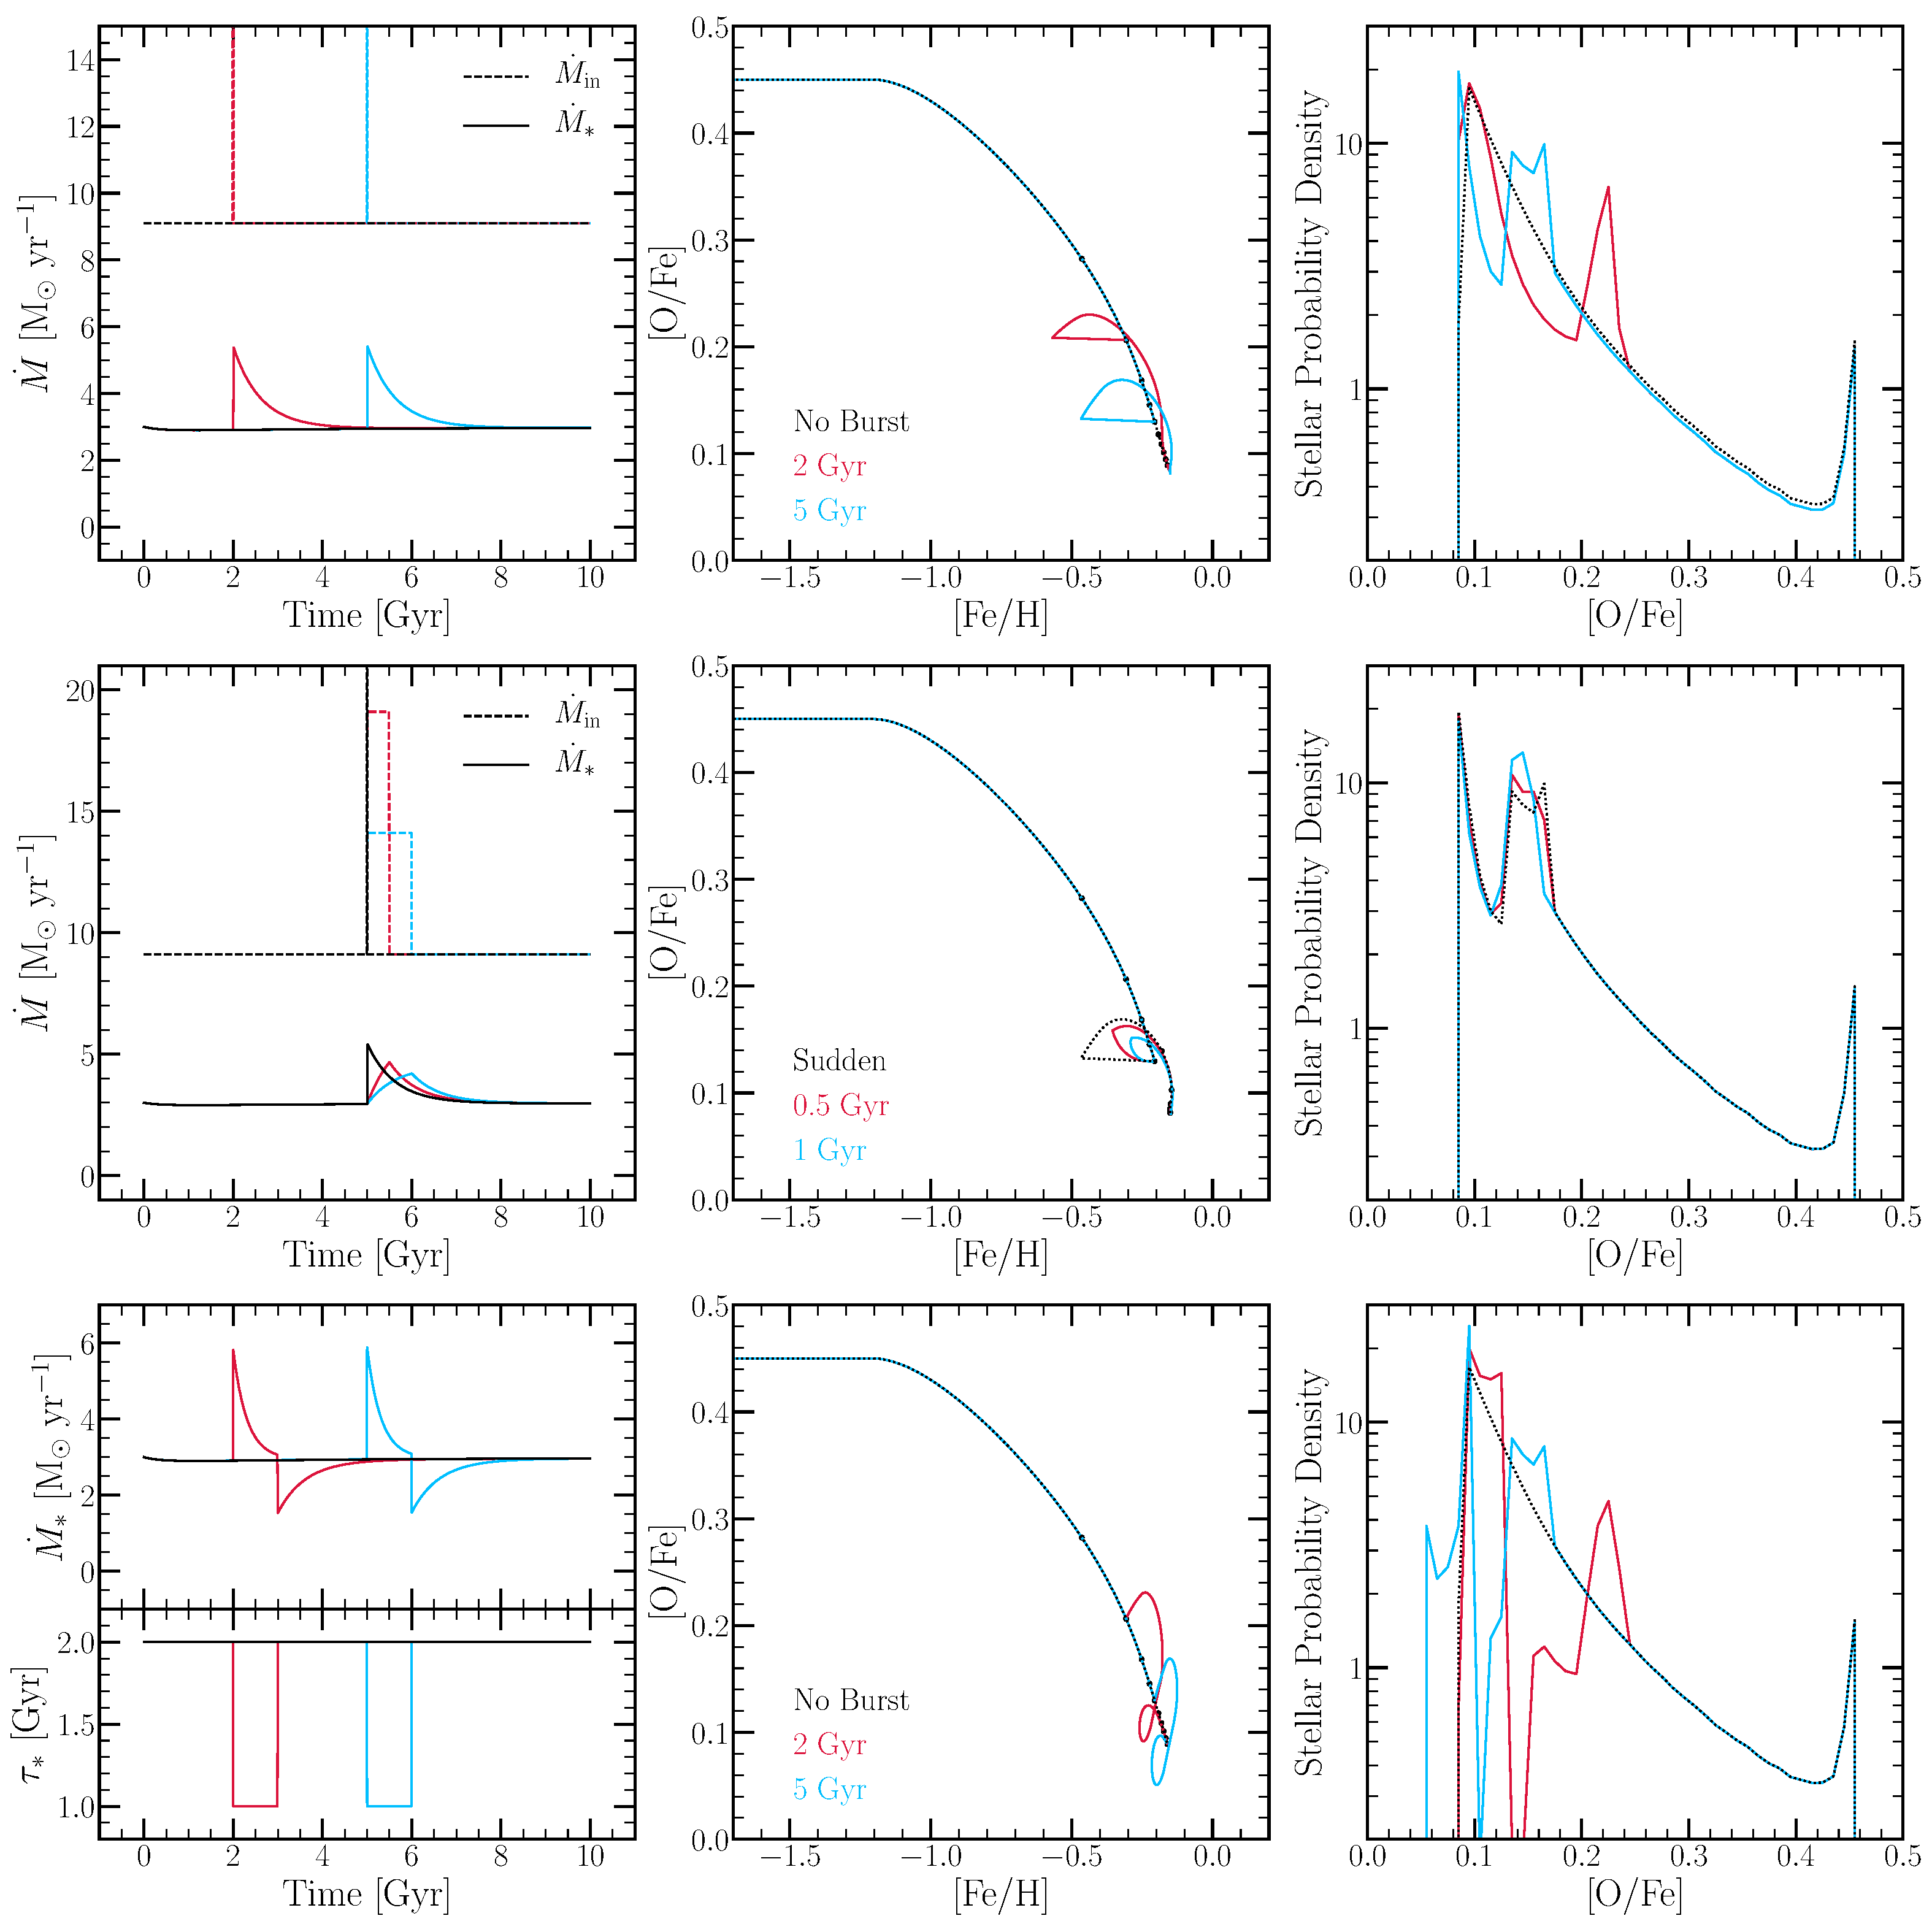
\includegraphics[scale = 0.31]{fiducial_bursts.pdf}
\caption{
Evolutionary tracks in the [O/Fe]-[Fe/H] plane (middle column) and [O/Fe] 
distributions (right column) of starburst GCE models with infall and star 
formation histories shown in left panels. \textbf{Top}: Black curves show an 
unperturbed model with a constant infall rate and near-constant star formation 
rate. Red and blue curves show models with starbursts induced by adding 85\% of 
the ISM mass worth of $Z = 0$ gas at $t = 2$ or $t = 5$ Gyr, 
respectively. \textbf{Middle}: Red and blue curves show models in which the 
gas infall rate is boosted over a time interval of $\Delta t$ = 0.5 Gyr or 1 
Gyr, respectively, at $t = 5$ Gyr. Black curves show the sudden gas infall 
model from the upper row for comparison. The total amount of gas added is the 
same in all three models. \textbf{Bottom}: Red and blue curves show models with 
starbursts induced by doubling the SFE (halving $\tau_*$) for an interval of 
$\Delta t = 1$ Gyr at $t = 2$ Gyr or 5 Gyr, respectively, with the infall rate 
(not plotted) held constant. Black curves show the unperturbed model. In the 
middle panels, small points on the unperturbed model curve mark 1 Gyr 
intervals. 
}
\label{bursts:fig:fiducial_cases}
\end{figure*} 

\begin{figure*} % fig 2
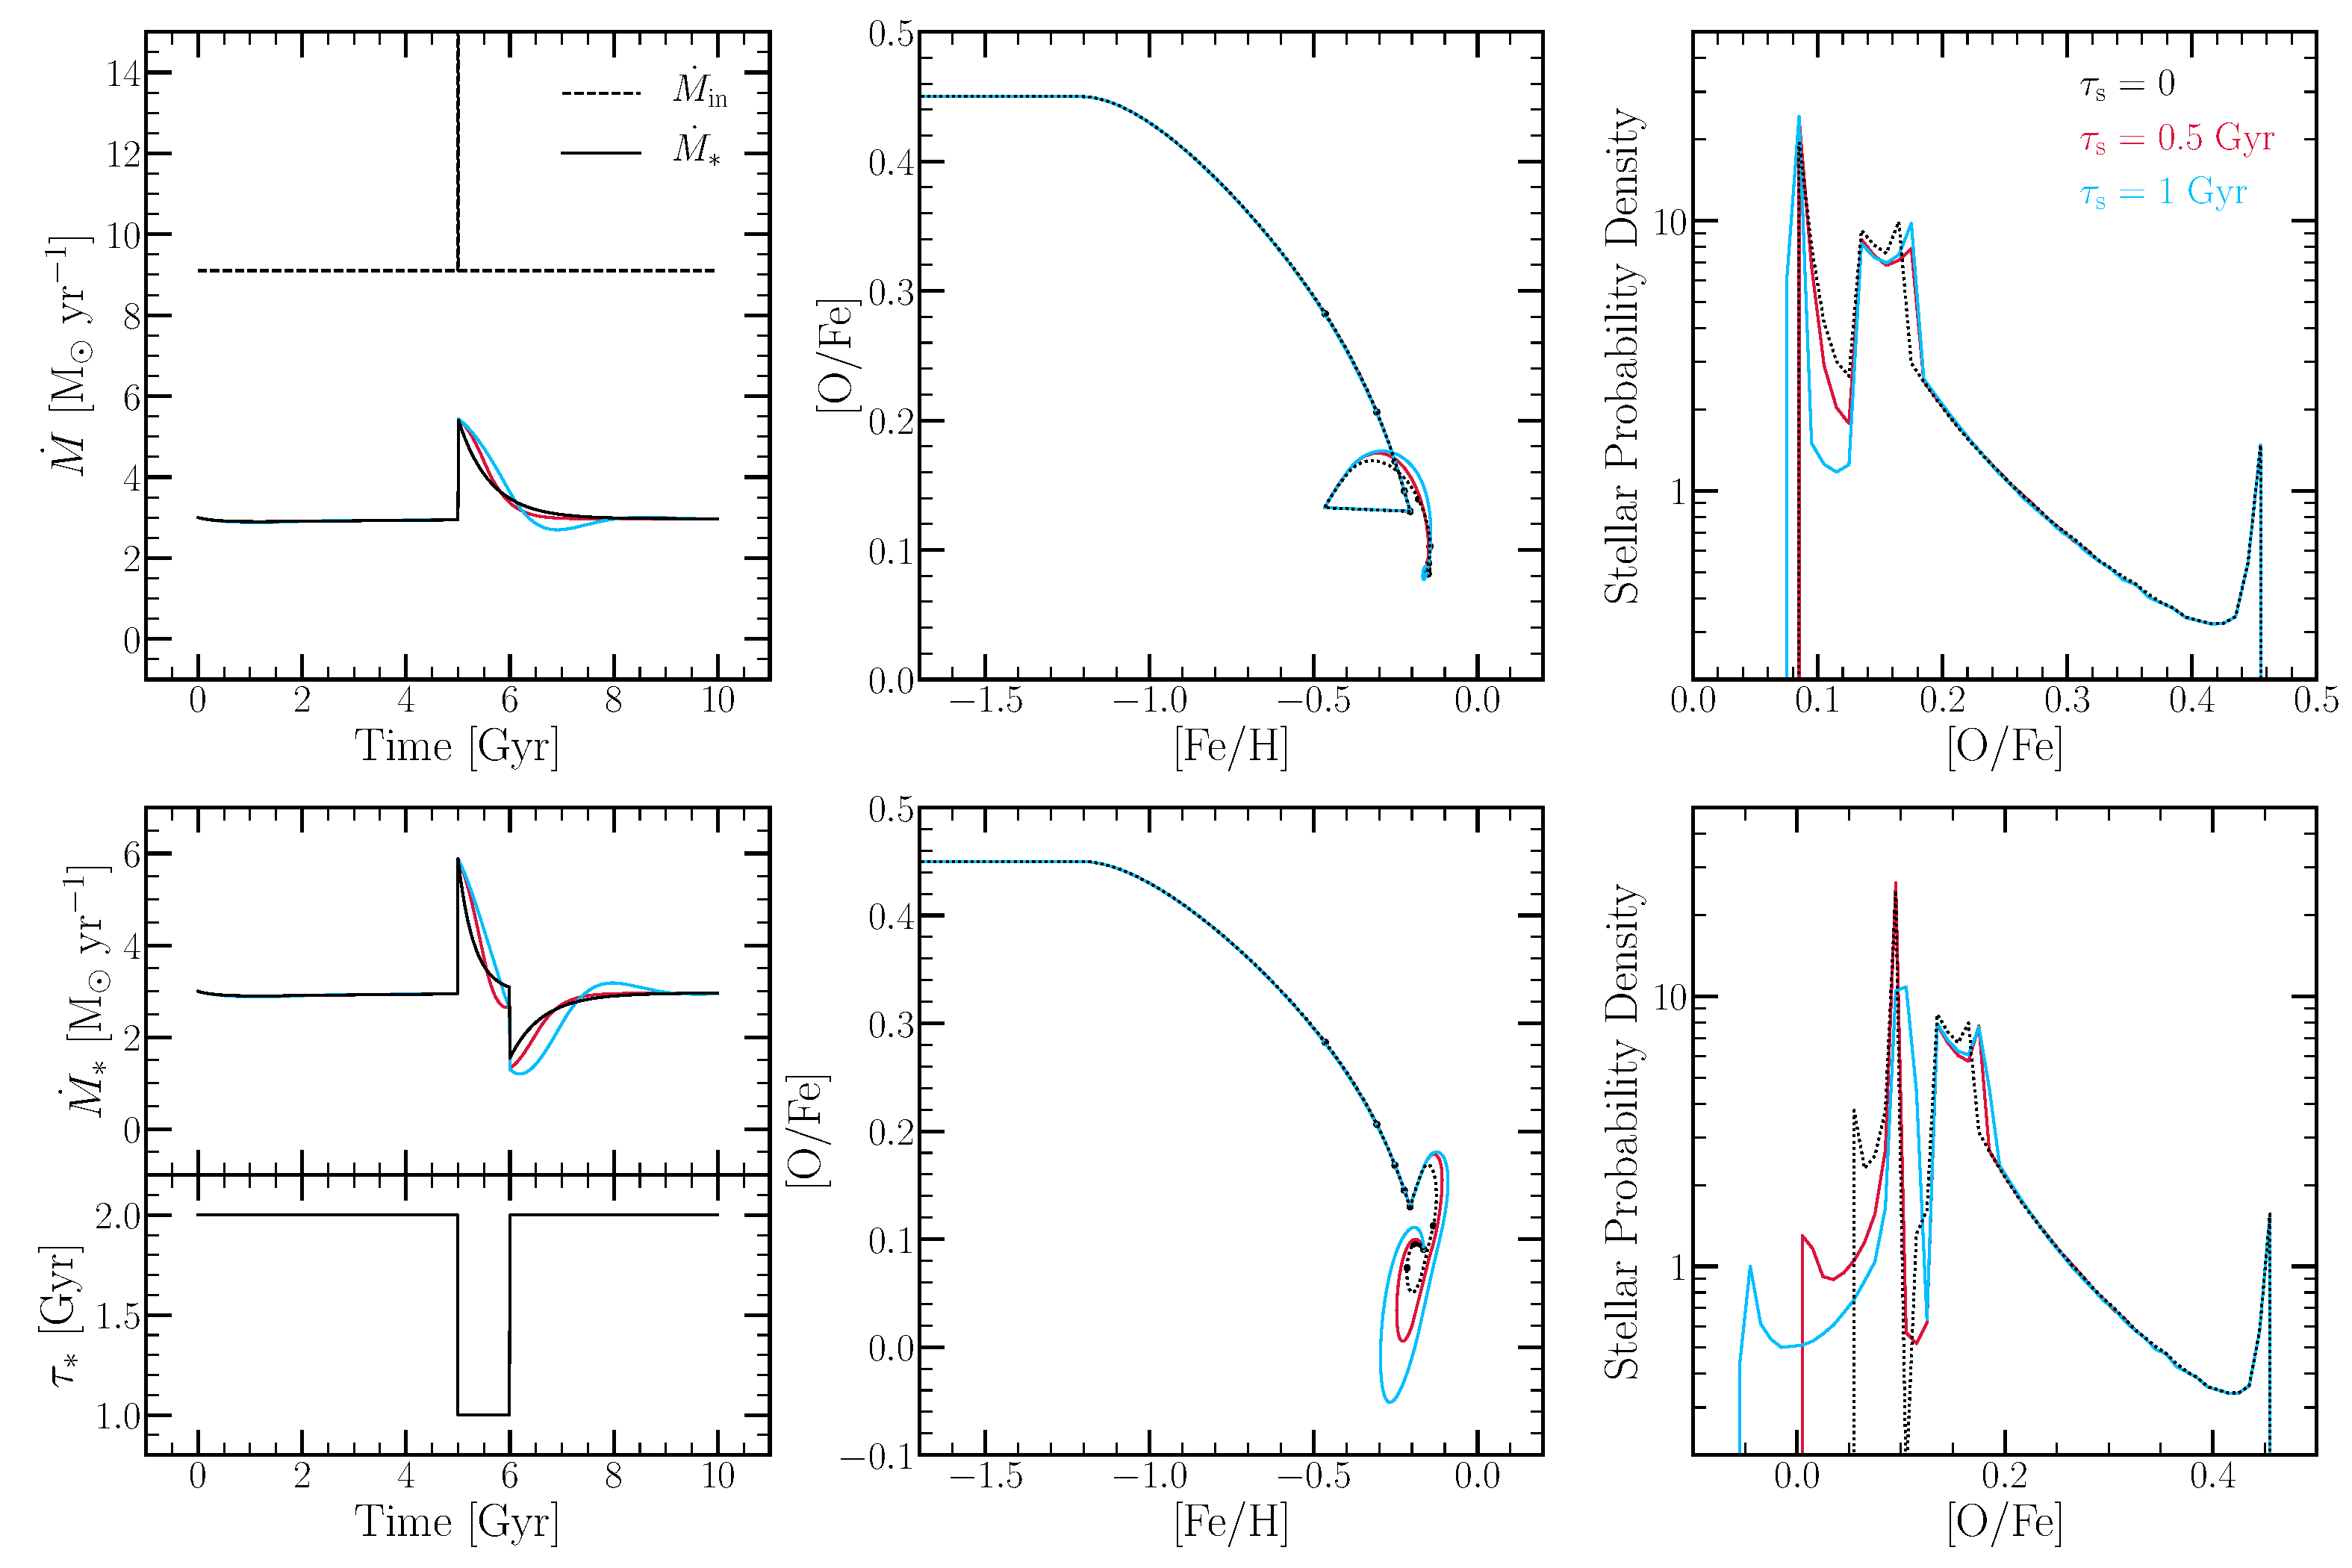
\includegraphics[scale = 0.31]{smoothing_time.pdf}
\caption{
Similar to Fig.~\ref{bursts:fig:fiducial_cases}, for models in which the outflow 
$\dot{M}_\text{out} = \eta\langle\dot{M}_*\rangle_{\tau_\text{s}}$ responds 
to the SFR averaged over a preceding interval $\tau_\text{s} = 0.5$ Gyr (red) 
or 1 Gyr (blue). Top and bottom rows show models in which the starburst is 
induced by increasing the gas supply or SFE, respectively, at $t = 5$ Gyr, as 
in the top and bottom rows of Fig.~\ref{bursts:fig:fiducial_cases}. Black dotted 
curves show the corresponding $\tau_\text{s} = 0$ models, repeated from 
Fig.~\ref{bursts:fig:fiducial_cases}, with small dots at 1 Gyr intervals in the 
middle panels.  
}
\label{bursts:fig:ts_combined}
\end{figure*} 

We begin by defining a GCE model with nearly constant star formation, which we 
will then perturb in a variety of ways. Our fiducial no-burst model has an 
infall rate of $\dot{M}_\text{in} = 9.1\ M_\odot\ \text{yr}^{-1}$ onto a galaxy 
with an initial gas supply of $M_\text{g} = 6.0\times10^9\ M_\odot$, an SFE 
timescale of $\tau_*$ = 2 Gyr, a mass-loading factor of $\eta$ = 2.5, 
$\tau_\text{s}$ = 0, and $\xi_\text{enh}$ = 1 (i.e. Z$_\text{out}$ = 
Z$_\text{gas}$) with continuous recycling. We also adopt a power-law SN Ia 
delay-time distribution (DTD) with R$_\text{Ia} \propto t^{-1.1}$ and minimum 
delay time of $t_\text{D}$ = 150 Myr. In short, this is a model with a 
constant infall rate and (nearly) constant star formation rate with parameters 
that do not change with time. The analytic model of~\citet{Weinberg2017b} 
accurately describes the [O/Fe] evolution of this numerical model. Although we 
adopt explicit numerical values for the initial gas mass and 
$\dot{M}_\text{in}$, the [Fe/H] and [O/Fe] evolution would be unchanged if we 
multiplied both of these quantities by the same constant factor. As shown 
by~\citet{Weinberg2017b}, the characteristic time for the evolution of O 
or other CCSN elements in such a model is the depletion time 
$\tau_\text{dep} \equiv \tau_*/(1 + \eta - r_\text{inst})$, while for Fe the 
evolutionary timescale depends on both $\tau_\text{dep}$ and the characteristic 
SN Ia timescale $\tau_\text{Ia}\sim 1-2$ Gyr. 

\subsection{Gas-Driven Starbursts}
\label{bursts:sec:gas-driven}

\begin{figure*} % fig 3
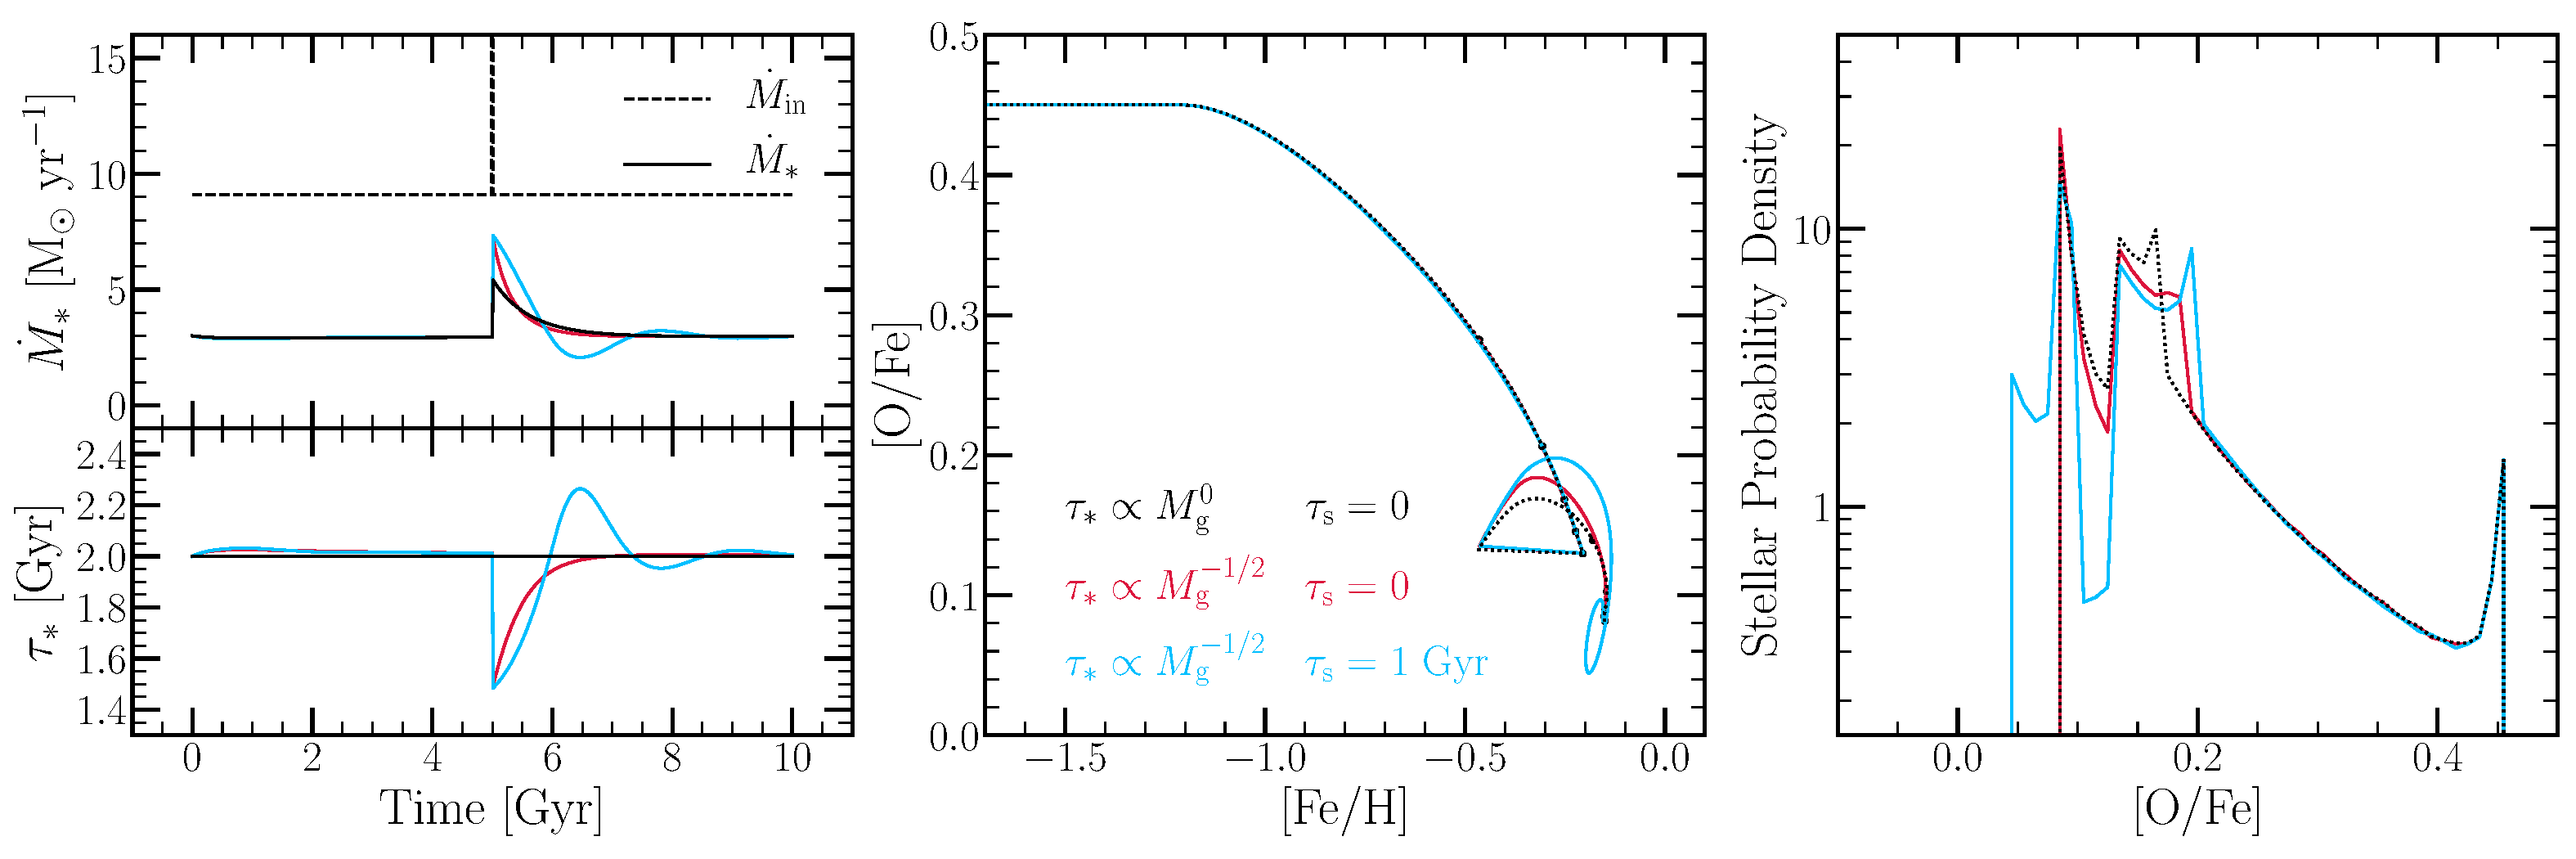
\includegraphics[scale = 0.31]{schmidt_smoothing.pdf}
\caption{
Similar to Fig.~\ref{bursts:fig:fiducial_cases}, for models in which the gas supply 
increases suddenly at $t = 5$ Gyr and the SFE timescale remains constant 
(black dotted) or decreases in accordance with the Kennicutt-Schmidt law (red, 
blue). The blue curve model has smoothing timescale $\tau_\text{s} = 1$ Gyr, 
and the black curve model is identical to the $t = 5$ Gyr starburst in the top 
row of Fig.~\ref{bursts:fig:fiducial_cases}. The lower left panel shows the response 
of $\tau_*$ to the evolving gas supply. 
}
\label{bursts:fig:ts_bolus_schmidt}
\end{figure*}

Our simplest starburst model is one in which a large amount of gas with a 
specified metallicity is added to the galaxy in a short amount of time. Here 
``large'' means that the added gas is significant compared to the current gas 
supply and ``short'' is relative to the timescales associated with GCE, in 
particular the depletion time $\tau_\text{dep}$. In this paper, we adopt the 
simplest scenario in which the added gas has zero metallicity, but any value 
can be used in \texttt{VICE}. 
\par
The top row of Fig.~\ref{bursts:fig:fiducial_cases} compares two gas-driven 
starburst models to our burstless scenario. These models have the same 
parameters as the burstless scenario with the exception of the infall rate. In 
these models, the infall rate assumes a value of $\dot{M}_\text{in}$ = 5000\ 
$M_\odot \text{yr}^{-1}$ for one $\Delta t$ = 1 Myr timestep, thereby adding 
$\dot{M}_\text{in}\Delta t = 5\times10^9 M_\odot$ of zero metallicity gas 
essentially instantaneously. Red and blue curves show models with gas added at 
$t = 2$ and $5$ Gyr, respectively. In each case, the nearly doubled gas supply 
causes a near doubling of the star formation rate (SFR). This burst decays on 
a timescale of~$\sim$1 Gyr as the excess gas is consumed by star formation and 
outflows. 
\par
The evolution of these models in [O/Fe] vs. [Fe/H] exhibits a ``jump-and-hook'' 
trajectory. Dilution by pristine gas causes an instantaneous jump to lower 
[Fe/H] at fixed [O/Fe]. The burst of star formation elevates the rate of CCSN 
enrichment to SN Ia enrichment, so the ISM evolves to higher [O/Fe] as the 
metallicity increases. Eventually the impact of the starburst dies away and 
the [O/Fe] evolution returns to that of the unperturbed model. 
\par 
The top right panel shows the normalized distribution of [O/Fe] in these 
models. The unperturbed model has two peaks in this distribution, the first at 
[O/Fe] $\approx$ +0.45 for stars formed early in the model galaxy's evolution 
when SN Ia enrichment is still negligible, and the second at 
[O/Fe] $\approx$ +0.08 produced when the system has reached equilibrium and is 
forming stars at constant [Fe/H] and [O/Fe]. For our adopted yields, a constant 
SFR model evolves to slightly super-solar [O/Fe], but a mildly declining SFR 
model would evolve to solar [O/Fe]~\citep[see][figure 3]{Weinberg2017b}. A 
declining SFR would also boost the equilibrium [Fe/H] to solar instead of 
mildly sub-solar for our adopted yields and $\eta$. We have chosen to focus on 
perturbations of a constant SFR model for simplicity, but we have checked that 
our qualitative conclusions hold if the underlying model has exponentially 
declining star formation with $\tau_\text{sfh}\approx$ 6 Gyr. 
\par 
The starburst models produce a third peak in this distribution at intermediate 
values of [O/Fe]. The lower edge of this peak corresponds to the value of 
[O/Fe] at the start of the burst, and the upper edge corresponds to the value 
of [O/Fe] at the top of the hook seen in the middle panel. The peak arises both 
because the system spends extra time at these [O/Fe] values and because the 
SFR is elevated during this time. Although the jump-and-hook trajectories are 
similar for the two starburst models, the arc in [O/Fe] is flatter for the 
earlier burst, which corresponds to a narrower peak in [O/Fe]. This difference 
arises because at $t$ = 2 Gyr the CCSN/SN Ia ratio of the unperturbed model is 
still elevated compared to its eventual equilibrium ratio, so the extra boost 
from the starburst has a smaller relative impact. 
\par 
A gas rich merger or violent dynamical disturbance may induce a very rapid 
increase in a galaxy's supply of star-forming gas. However, a temporary boost 
in a galaxy's gas accretion rate can also induce elevated star formation. 
The middle row of Fig.~\ref{bursts:fig:fiducial_cases} compares the $t = 5$ Gyr 
instantaneous gas increase model to models in which the same 
$5\times10^9 M_\odot$ of gas is added over $\Delta t$ = 0.5 and 1.0 Gyr 
intervals. The perturbation to the SFR is smoother (left panel), though the 
number of ``extra'' stars formed is similar. The hooks in [O/Fe]-[Fe/H] are no 
longer flat-bottomed because the elevated SFR increases [O/Fe] at the same 
time that the infall dilutes [Fe/H]. For $\Delta t$ = 1 Gyr the jump in [O/Fe] 
is small because the maximum boost of SFR is only about half that of the 
instantaneous model. However, the extra peak in the [O/Fe] distribution is 
remarkably similar in all three models, though slightly sharper for 
$\Delta t$ = 1 Gyr. 
Although their model differs in detail, these findings are in good qualitative 
agreement with the ``two-infall'' model predictions presented 
in~\citet{Spitoni2019}. 
\par 
We conclude that a third peak in the [O/Fe] distribution is the characteristic 
observable signature of a gas-driven starburst that formed a significant 
fraction of a system's stars. The location of the peak indicates the value of 
[O/Fe] at the time of the burst. Resolving these peaks requires a large sample 
of stars with precise [O/Fe] (or [$\alpha$/Fe]) values, i.e. statistical errors 
of 0.05 dex or below. Correlating these [$\alpha$/Fe] measurements with 
individual stellar age estimates could increase the diagnostic power even if 
the age estimates have substantial statistical errors. 


\subsection{Efficiency-Driven Starbursts}
\label{bursts:sec:efficiency-driven}
The bottom row of Fig.~\ref{bursts:fig:fiducial_cases} shows a scenario in which 
starbursts arise from a temporary increase of SFE instead of an increase in 
gas supply. We double the SFE -- thus decreasing the SFE timescale $\tau_*$ 
from 2 Gyr to 1 Gyr -- for a period of $\Delta t$ = 1 Gyr, beginning at $t = 2$ 
or 5 Gyr. The gas infall rate is held constant. As in the gas-doubling 
scenario, the SFR initially jumps by a factor of two, then decays to its 
original value. However, once $\tau_*$ returns to 2 Gyr, the SFR drops 
\textit{below} that of the unperturbed model because the gas supply has been 
depleted during the high SFE phase. Over an interval of~$\sim$1 Gyr, the SFR 
recovers to the value of $\dot{M}_*\approx3\ M_\odot\ \text{yr}^{-1}$ at which 
star formation and outflow balance infall. 
\par 
The hooks in [O/Fe]-[Fe/H] evolution have a different morphology for the 
efficiency-driven bursts. Because there is no dilution by low metallicity gas, 
the tracks jump up to higher [O/Fe] with slightly increasing [Fe/H], instead 
of first moving back to lower [Fe/H]. Furthermore, because of the depression 
in SFR once $\tau_*$ returns to its baseline value, the [O/Fe] track dips 
below that of the unperturbed model before returning to it at late 
times. During the downward loop, the rate of SNe Ia is high because of the 
stars formed during the recent burst, but the rate of CCSNe is low due to the 
reduced SFR. 
\par 
The distribution of [O/Fe] in these models again shows an extra peak at [O/Fe] 
values close to those at the onset of the starburst. However, the morphology 
of these distributions is different from that of the gas-driven starburst 
models in two ways. First, the peak in [O/Fe] is followed by a much deeper 
trough at slightly lower [O/Fe] because the SFR is depressed while the ISM is 
evolving through this abundance ratio. Second, the [O/Fe] distribution 
acquires an additional peak at a value that corresponds to the bottom of the 
downward loops in the middle panel. With sufficiently good data, it might be 
possible to distinguish the signature of gas-driven and efficiency-driven 
starbursts from the detailed shape of the [O/Fe] distribution. In particular, 
an efficiency-driven burst at relatively late times would produce a population 
of roughly coeval stars with [$\alpha$/Fe] values below that of the bulk 
population. There is some hint of such a population in the solar 
neighborhood~\citep{Feuillet2018}. 

\subsection{Outflow Smoothing Time}
\label{bursts:sec:smoothing}
We now examine models in which the outflow rate $\dot{M}_\text{out}$ responds 
to the SFR averaged over a time interval $\tau_\text{s}$ instead of the 
instantaneous SFR. Fig.~\ref{bursts:fig:ts_combined} shows star formation histories, 
[O/Fe]-[Fe/H] tracks, and [O/Fe] distributions for gas-driven and 
efficiency-driven starburst models with $\tau_\text{s}$ = 0, 0.5, and 1 Gyr. 
The $\tau_\text{s}$ = 0 models are identical to the t = 5 Gyr burst models 
shown in the top and bottom rows of Fig.~\ref{bursts:fig:fiducial_cases}. Because 
the enhanced infall models (middle row of Fig.~\ref{bursts:fig:fiducial_cases}) are 
qualitatively similar to the instantaneous gas doubling model (top row), we 
show only this limiting case of a gas-driven starburst in the remainder of the 
paper. 
\par 
For the gas-driven starburst, even a 1 Gyr smoothing time has only a small 
impact on the [O/Fe]-[Fe/H] trajectory and [O/Fe] distribution. Just after the 
accretion event, the SFR in the smoothed models is slightly higher than in the 
$\tau_\text{s}$ = 0 model because the outflow rate is lower, and the hook in 
the evolutionary track therefore reaches slightly higher [O/Fe]. For 
$\tau_\text{s}$ = 1 Gyr, the SFR at $t\approx$ 6 - 8 Gyr dips below the 
3 $M_\odot\ \text{yr}^{-1}$ baseline, because the extra accreted gas has been 
consumed and the outflow rate remains high because of the earlier starburst. 
As a result, the deficit in the [O/Fe] distribution at [O/Fe] $\approx$ +0.1 
is deeper in this model. 
\par 
For the efficiency-driven starburst, smoothing has a larger impact because the 
delayed outflow deepens the depression of SFR after the burst. The downward 
hook of [O/Fe] is therefore substantially deeper even for $\tau_\text{s}$ = 0.5 
Gyr. Smoothing of the outflow response exaggerates the characteristic form of 
an efficiency-driven starburst perturbation and moves the extra peak of the 
[O/Fe] distribution to a lower value. 


\subsection{Hybrid Starbursts}
\label{bursts:sec:hybrid}
If the gas supply of a galaxy increases suddenly, then the SFE may also 
increase because of greater gas self-gravity, more rapid cloud collisions, or 
whatever dynamical disturbance drove the gas increase in the first place. 
Observations provide some evidence for starbursts that are driven by both 
increased gas supply and increased 
SFE~\citep[][and the citations therein]{Kennicutt2012}. 
Fig.~\ref{bursts:fig:ts_bolus_schmidt} shows results for a hybrid model in which a 
doubling of the gas supply is linked to a Kennicutt-Schmidt scaling of the SFE, 
with $\tau_* = (2\text{ Gyr})(M_\text{g}/6\times10^9\ M_\odot)^{-1/2}$ (see 
\S~\ref{bursts:sec:methods}). If the smoothing time $\tau_\text{s}$ = 0, then the 
evolution of this hybrid model is only slightly different from that of our 
standard gas-driven starburst, as one can see by comparing the dashed black and 
solid red curves in the middle and right panels of 
Fig.~\ref{bursts:fig:ts_bolus_schmidt}. The hybrid burst has a higher peak SFR, 
which leads to a higher peak of the [O/Fe] hook. For $\tau_\text{s}$ = 1 Gyr, 
the trajectory and [O/Fe] distribution of the hybrid model show features of 
both the gas-driven and efficiency-driven models. In particular, this model 
has a period of depressed SFR because of the delayed ejection of gas by the 
starburst, and the enhanced ratio of SNe Ia/CCSNe during this period causes a 
downward hook in [O/Fe] and an additional peak in the [O/Fe] distribution. 



\section{Strontium}
\label{bursts:sec:sr}
\subsection{Nucleosynthesis}
\label{bursts:sec:sr_nuc}

\begin{figure} % fig 4
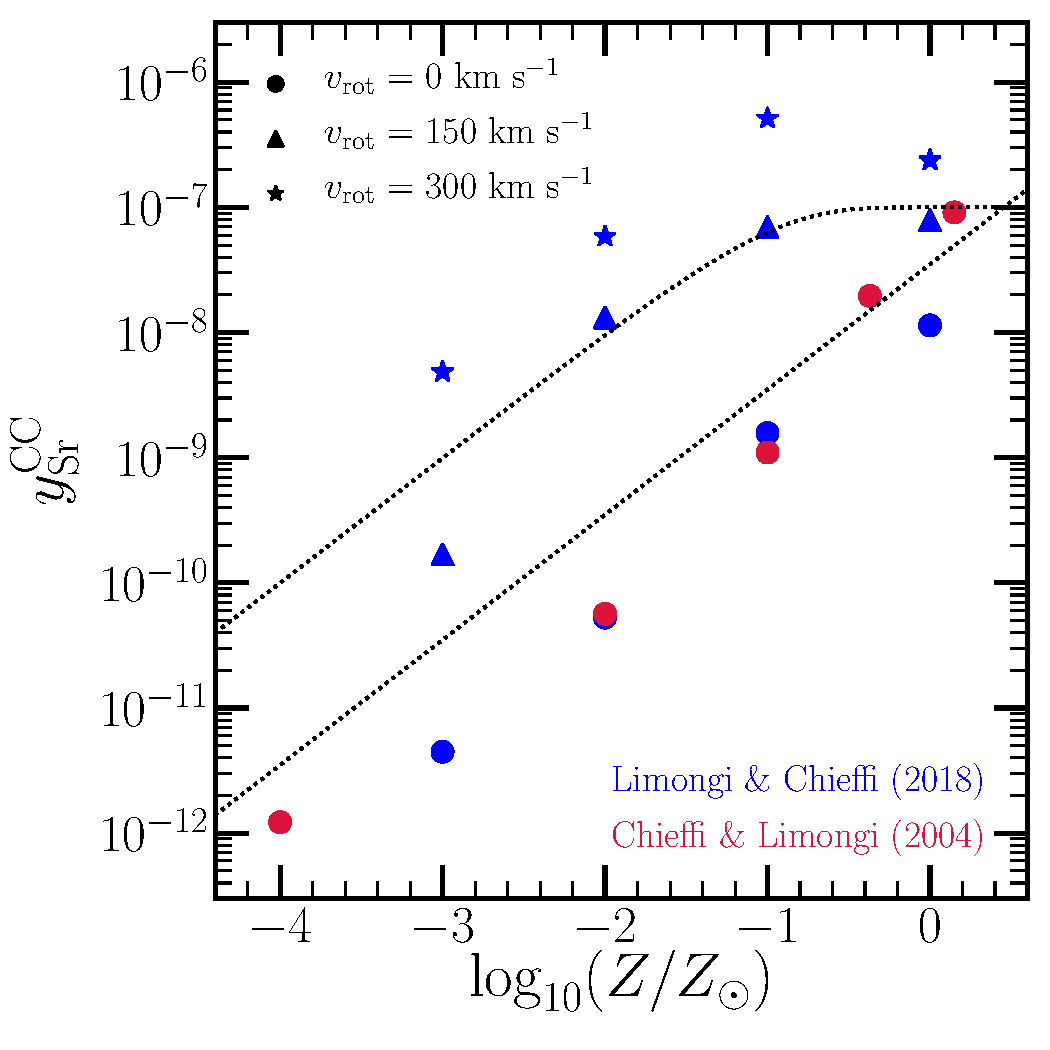
\includegraphics[scale = 0.45]{sr_cc_yields.pdf}
\caption{
IMF-averaged CCSN yields of Sr computed using the non-rotating progenitor 
models of (\citealp{Chieffi2004}, red circles) and the models 
of~\citet{Limongi2018} for progenitors with $v_\text{rot} = 0$ (blue circles), 
150 km s$^{-1}$ (blue triangles), and 300 km s$^{-1}$ (blue stars). Dotted 
curves show approximate characterizations of these results used in our GCE 
models, $y_\text{Sr}^\text{CC} = 3.5\times10^{-8}(Z/Z_\odot)$ and 
$y_\text{Sr}^\text{CC} = 10^{-7}(1 - \exp{(-10Z/Z_\odot)})$. We adopt $Z_\odot$ = 
0.014 based on~\citet{Asplund2009}. 
}
\label{bursts:fig:sr_cc_yields}
\end{figure} 

\begin{figure*} % fig 5
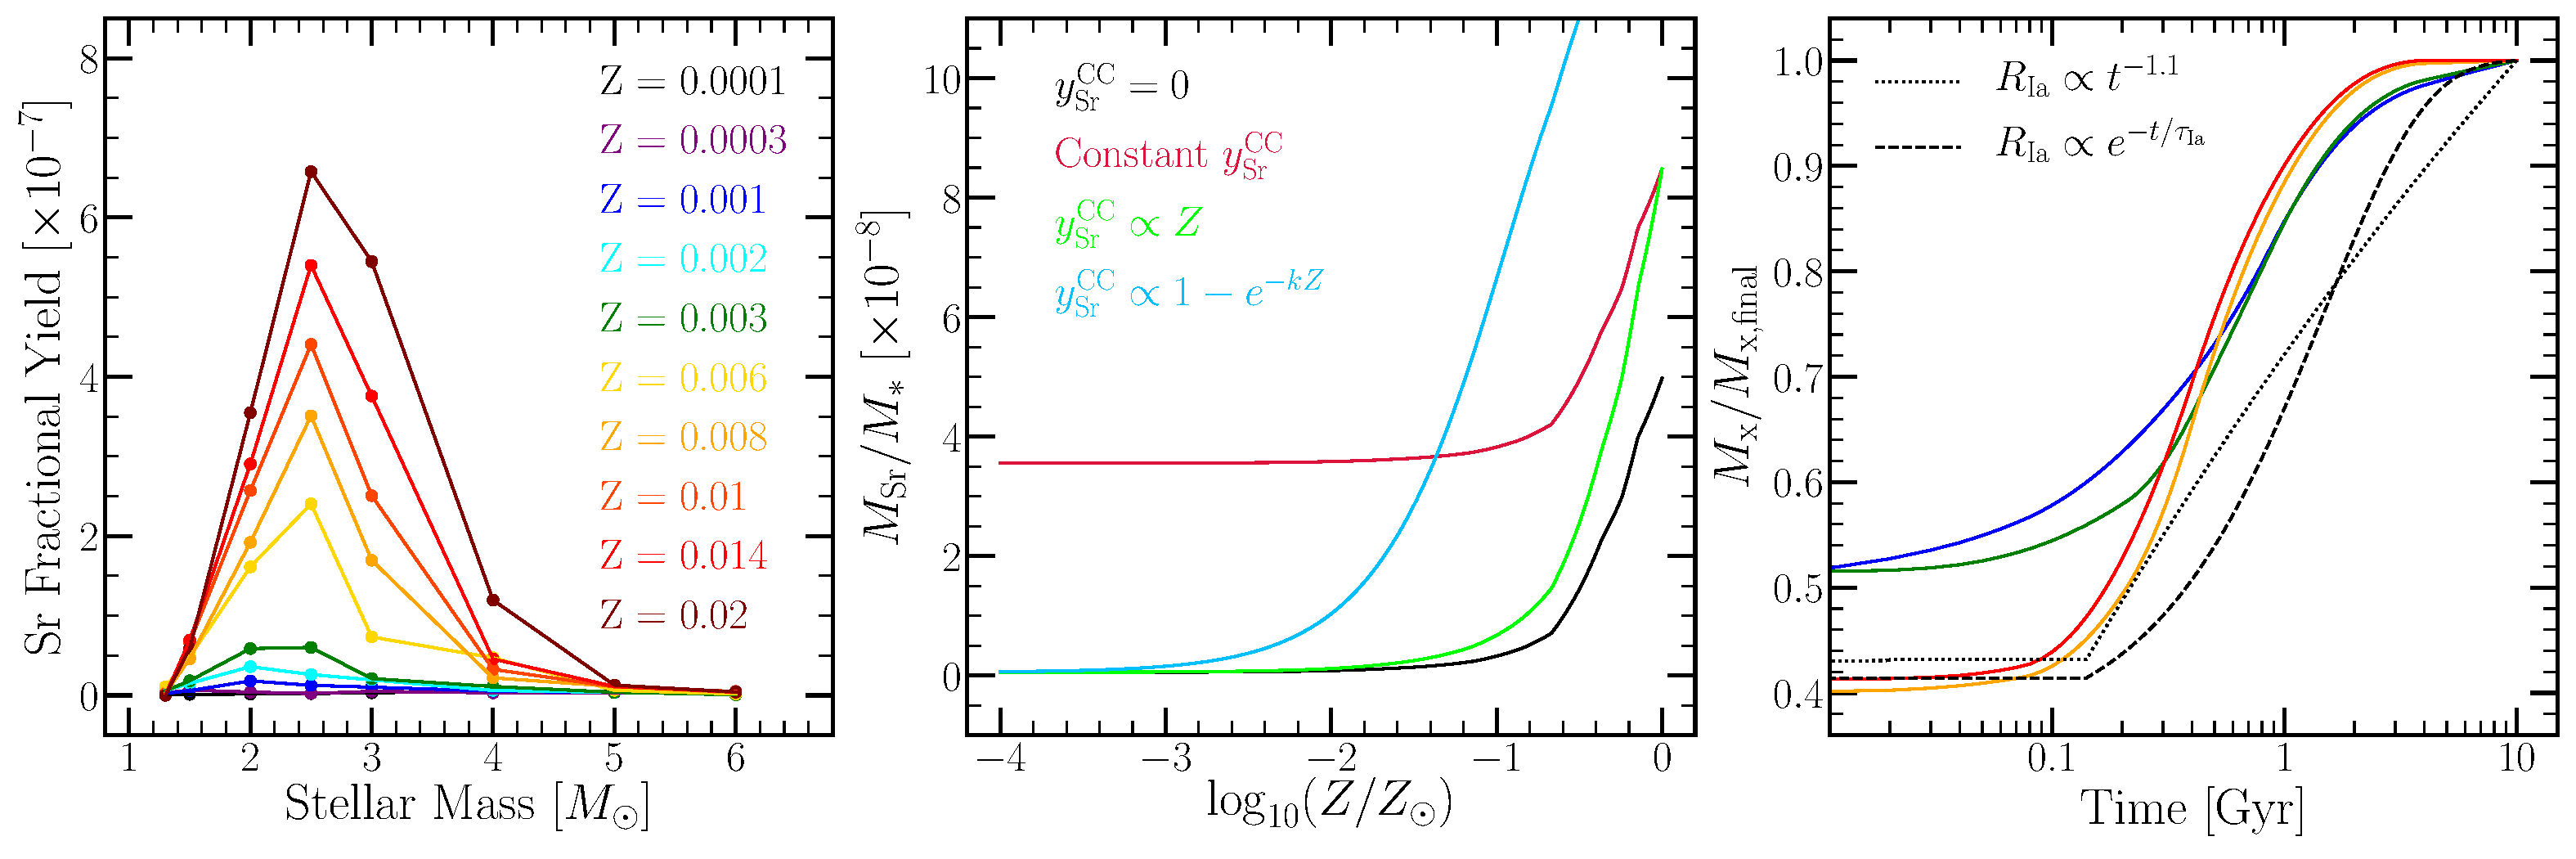
\includegraphics[scale = 0.32]{sr_yields_ssp.pdf}
\caption{
Yields of Sr as a function of stellar mass, metallicity, and time. 
\textbf{Left}: Fractional yields of AGB stars - the ejected Sr mass divided by 
the initial stellar mass, computed as a function of stellar mass and 
metallicity using the FRANEC code~\citep{Cristallo2011}. \textbf{Middle}: 
IMF-averaged Sr yield after 10 Gyr, for a single stellar population of 
metallicity $Z$ formed at $t = 0$, computed by adding the AGB yields to CCSN 
yields illustrated by the dotted curves in Fig.~\ref{bursts:fig:sr_cc_yields}, or to 
constant yields $y_\text{Sr}^\text{CC} = 3.5\times10^{-8}$ or 
$y_\text{Sr}^\text{CC} = 0$ (AGB only). \textbf{Right}: Time evolution of Sr 
production for single stellar populations of metallicity $Z$ = 0.001, 0.003, 
0.008, and 0.014, assuming the $y_\text{Sr}^\text{CC} \propto Z$ model. 
Curves are color-coded to the legend in the left panel. All curves are 
normalized to the final Sr mass produced after 10 Gyr, which depends strongly 
on $Z$ as shown in the right panel. Dotted and dashed black curves show the 
time evolution of Fe for our standard values of $y_\text{Fe}^\text{CC}$ and 
$y_\text{Fe}^\text{Ia}$ and a $t^{-1.1}$ or $e^{-t/1.5\text{ Gyr}}$ DTD with a 
minimum delay time of 0.15 Gyr. Because AGB production is dominated by 
$2-4\ M_\odot$ stars, AGB Sr enrichment from a single stellar population 
occurs faster than SN Ia Fe enrichment.  
}
\label{bursts:fig:sryields_3panel}
\end{figure*}

Strontium is one of the commonly used tracers of s-process nucleosynthesis in 
AGB stars~\citep[e.g.][]{Conroy2013a, Mishenina2019}. Sr production differs from 
that of O and Fe, the two elements that we have examined thus far, because the 
delay time of AGB enrichment differs from that of SNe Ia and because the Sr 
yields of both CCSNe and AGB stars are expected to depend strongly on 
metallicity. Both of these differences have an important impact on predicted 
evolutionary tracks and element ratio distributions. 
\par 
Fig.~\ref{bursts:fig:sr_cc_yields} plots IMF-averaged net CCSN yields of strontium 
based on the models of~\citet{Chieffi2004} and~\citet{Limongi2018}. 
These are the solutions to equation~\refp{bursts:eq:frac_yield} with the 
same IMF parameters discussed in~\S~\ref{bursts:sec:ccsne}.


\citet{Chieffi2004} report Sr yields for non-rotating CCSN progenitors 
($v_\text{rot}$ = 0) at a wide range of metallicities, while \citet{Chieffi2013} 
report yields for $v_\text{rot}$ = 0 and 300 km s$^{-1}$ but at only solar 
metallicity. Progenitor rotation affects Sr yields from CCSNe due to 
rotationally induced mixing~\citep{Frischknecht2016}. We presume the results 
of~\citet{Chieffi2013} to be superseded by those of~\citet{Limongi2018}, who 
examined a range of metallicites and values of $v_\text{rot}$ = 0, 150 km 
s$^{-1}$, and 300 km s$^{-1}$. However, we caution that the impact of rotation 
on the Sr yield at solar metallicity is much stronger in 
the~\citet{Limongi2018} study than in~\citet{Chieffi2013} due to a different 
calibration of the rotation-induced mixing efficiency. 
\par 
Fig.~\ref{bursts:fig:sr_cc_yields} shows that the predicted CCSN yields depend 
strongly on metallicity and are much higher (typically 1-3 orders of magnitude) 
for rapidly rotating vs. non-rotating progenitors. As approximate descriptions 
of the numerical results, we show the functions 
\begin{subequations}\begin{align} 
y_\text{Sr}^\text{CC} &= 3.5\times10^{-8}(Z / Z_\odot) 
\label{bursts:eq:y_sr_cc_linear} \\ 
\intertext{for v$_\text{rot}$ = 0 and} 
y_\text{Sr}^\text{CC} &= 10^{-7}\left[1 - e^{-10(Z/Z_\odot)}\right] 
\label{bursts:eq:y_sr_cc_limexp} 
\end{align}\end{subequations} 
for $v_\text{rot}$ = 150 km s$^{-1}$. For comparison, we will also compute GCE 
models with a constant $y_\text{Sr}^\text{CC} = 3.5\times10^{-8}$ matched to 
our linear model at $Z = Z_\odot$ and with $y_\text{Sr}^\text{CC} = 0$ 
corresponding to pure AGB enrichment. We caution that these are not fits to 
the yields plotted in Fig.~\ref{bursts:fig:sr_cc_yields}; we adopt them as an 
agnostic approach to the form of the metallicity-dependent yield in the 
interval -2 $\lesssim$ [Fe/H] $\lesssim$ 0 in which our models are focused. 
\par
For AGB production of Sr, we use fractional yields as a function of initial 
stellar mass at various metallicities from the FRANEC 
code~\citep{Cristallo2011}. These are plotted in the left-hand panel of 
Fig.~\ref{bursts:fig:sryields_3panel}, and they show two notable features. First, 
for near-solar metallicity the fractional yields are sharply peaked at stellar 
masses of 2-3 $M_\odot$. To obtain the total mass yield per star one 
multiplies by $M$, giving weight to the contribution of higher mass 
stars, but the number of stars per linear $\Delta M$ interval is proportional 
to $M^{-2.3}$ for a Kroupa IMF in this mass range, thus increasing the weight 
of lower mass stars. The strong mass dependence of the fractional yields means 
that the IMF-averaged AGB yield is dominated by stars with relatively short 
lifetimes. The second notable feature is a strong metallicity dependence, 
expected because the amount of Sr produced via the s-process during the AGB 
phase should increase with the abundance of free neutrons produced by nuclear 
reactions involving C and Ne isotopes. For $Z\lesssim Z_\odot/3$ the predicted 
fractional yields are below $10^{-7}$ at all masses, and for 
$Z\gtrsim Z_\odot/3$ the maximum fractional yield is roughly proportional to 
$Z$. 
\par 
In the middle panel of Fig.~\ref{bursts:fig:sryields_3panel}, the black curve shows 
the late-time ($t = 10$ Gyr), IMF-averaged AGB Sr yield as a function of 
metallicity. At $Z = Z_\odot$, the yield is $y_\text{Sr}^\text{AGB} = 
5\times10^{-8}$, but for $Z < Z_\odot/3$ the yield is well below $10^{-8}$. 
The green curve shows the total yield from adding $y_\text{Sr}^\text{AGB}$ to 
the $y_\text{Sr}^\text{CC}$ of equation~\refp{bursts:eq:y_sr_cc_linear}, which 
approximates the non-rotating~\citet{Limongi2018} models. At all metallicities 
for which $y_\text{Sr} > 10^{-8}$, the CCSN and AGB contributions are 
comparably important. However, for the $v_\text{rot} = 150\text{ km s}^{-1}$ 
yields approximated by equation~\refp{bursts:eq:y_sr_cc_limexp}, the CCSN yields 
dominate over the AGB yields at all metallicities (blue curve). The red curve 
shows the simple case of adding $y_\text{Sr}^\text{AGB}$ to a constant 
$y_\text{Sr}^\text{CC} = 3.5\times10^{-8}$. 

\begin{figure*} % fig 6 
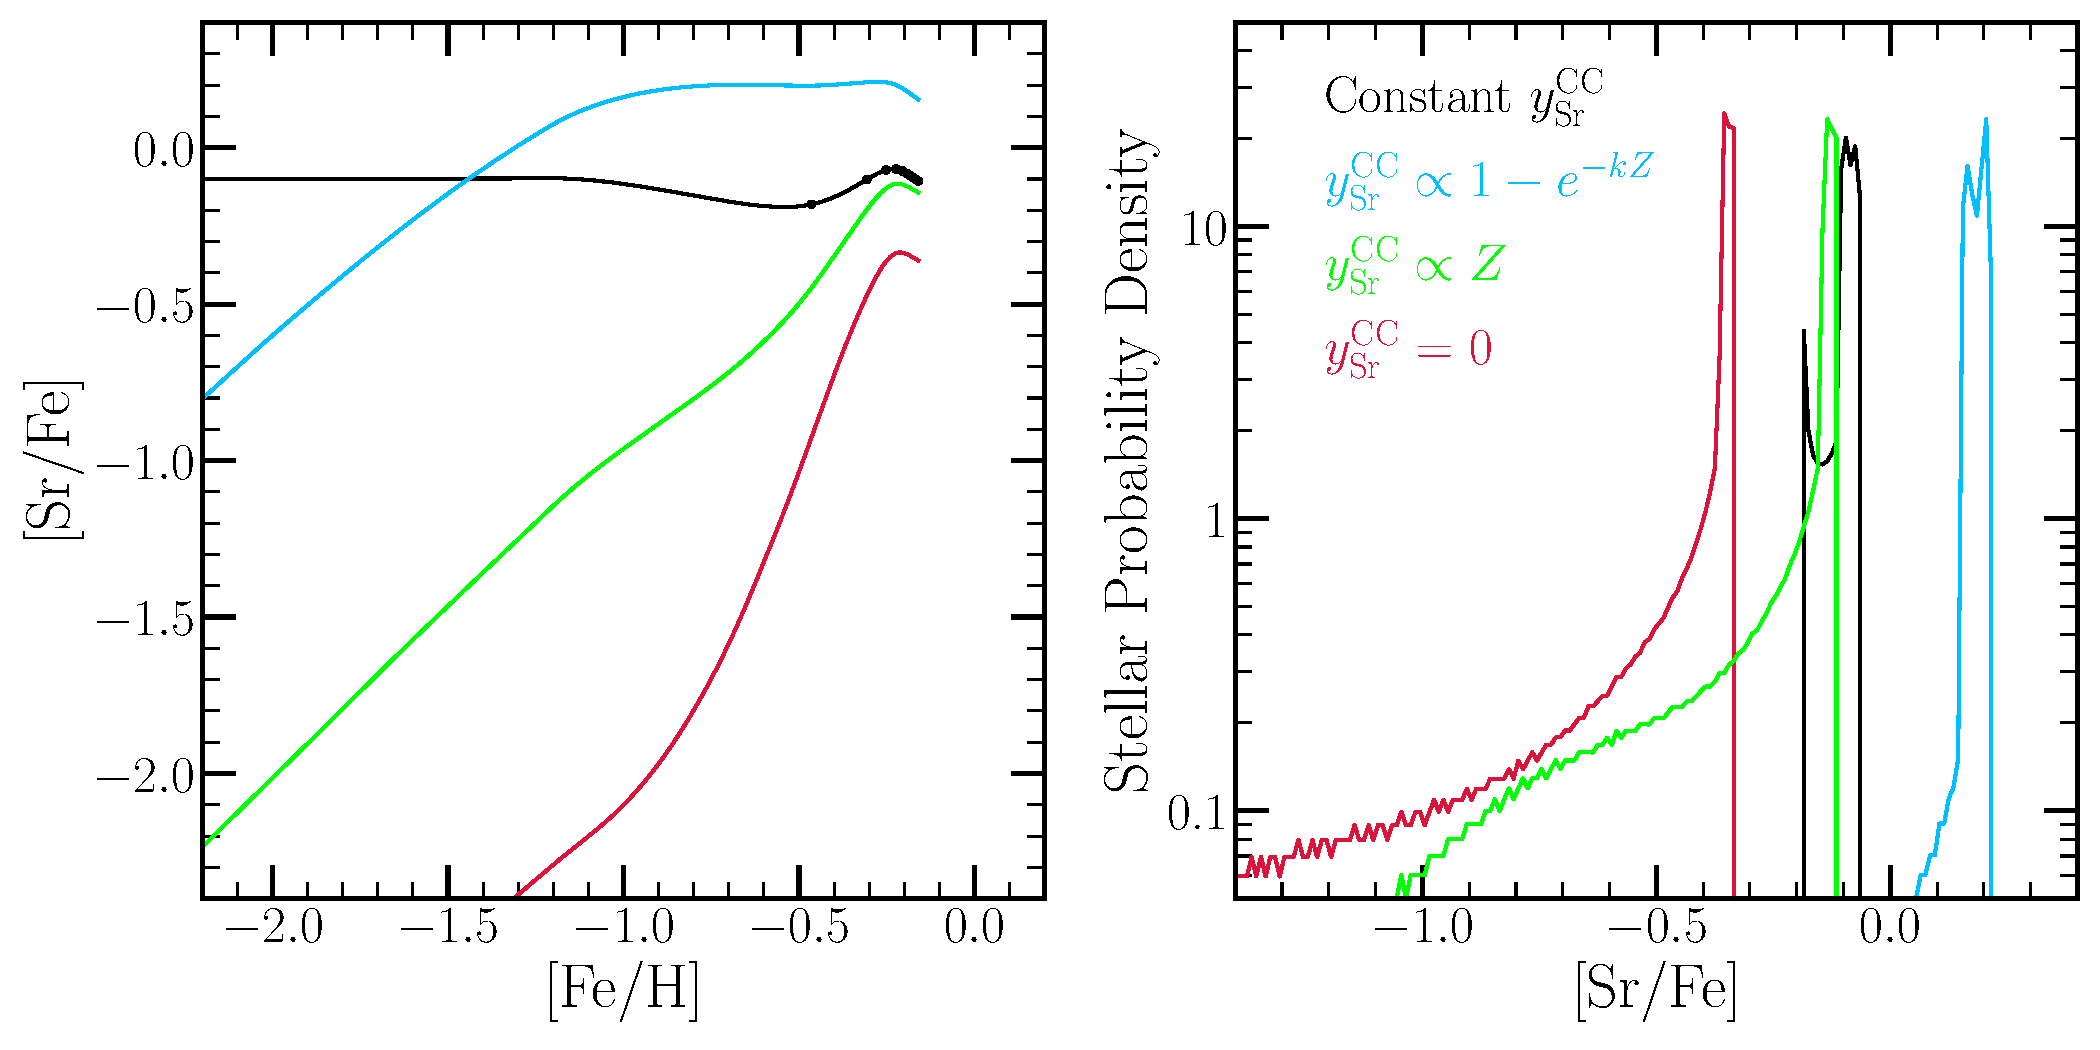
\includegraphics[scale = 0.45]{sr_yield_assumptions.pdf}
\caption{
Evolutionary tracks (left) and final [Sr/Fe] distributions (right) under our 
fiducial burstless GCE model for four different assumptions about 
$y_\text{Sr}^\text{CC}$: constant yield, zero yield, and the 
metallicity-dependent yields for non-rotation or rotation progenitors 
described by equations~\refp{bursts:eq:y_sr_cc_linear} and~\refp{bursts:eq:y_sr_cc_limexp}. 
The red ($y_\text{Sr}^\text{CC} = 0$) curve shows the predicted evolution for 
our metallicity dependent AGB yields (\citealp{Cristallo2011}; 
Fig.~\ref{bursts:fig:sryields_3panel}), which are adopted in all four models. On the 
black curve, small black points are plotted at $\Delta t$ = 1 Gyr intervals, 
and all models reach a given [Fe/H] at the same time. 
}
\label{bursts:fig:sr_yields}
\end{figure*}

The right panel of Fig.~\ref{bursts:fig:sryields_3panel} shows the time evolution of 
Sr production for a selection of metallicity values shown in the left panel, 
$Z$ = 0.001, 0.003, 0.008, and 0.014. All curves are normalized by the 
late-time yield, which is strongly dependent on metallicity as shown in the 
middle panel. Here we adopt the $y_\text{Sr}^\text{CC} \propto Z$ yield model 
for CCSNe, and in all cases this accounts for about 40-50\% of the total yield. 
Typically about half of the AGB contribution comes within the first 0.5 Gyr, 
and nearly all of it within 2 Gyr. Dotted and dashed curves show the evolution 
of Fe production for our fiducial values of $y_\text{Fe}^\text{CC} = 0.0012$ 
and $y_\text{Fe}^\text{Ia} = 0.0017$ and a $t^{-1.1}$ DTD or an 
$e^{-t/1.5\text{ Gyr}}$ DTD, respectively. Although our assumed minimum delay 
is $t_\text{D} = 0.15$ Gyr, getting half of the SN Ia Fe contribution 
takes~$\sim0.9 - 1$ Gyr, so the AGB Sr enrichment is faster, albeit moderately, 
than the SN Ia Fe enrichment. This rapid AGB contribution is a consequence of 
the dominant contribution from $2 - 4\ M_\odot$ stars, which have short 
lifetimes. These curves represent the Sr production from a single population of 
stars at a given metallicity. In a GCE model the metallicity itself rises with 
time, thus increasing the Sr production because of the metallicity-dependent 
yield. In the next section, we demonstrate that this complicates the 
enrichment timescale of Sr relative to Fe. 

\begin{figure*} % fig 7
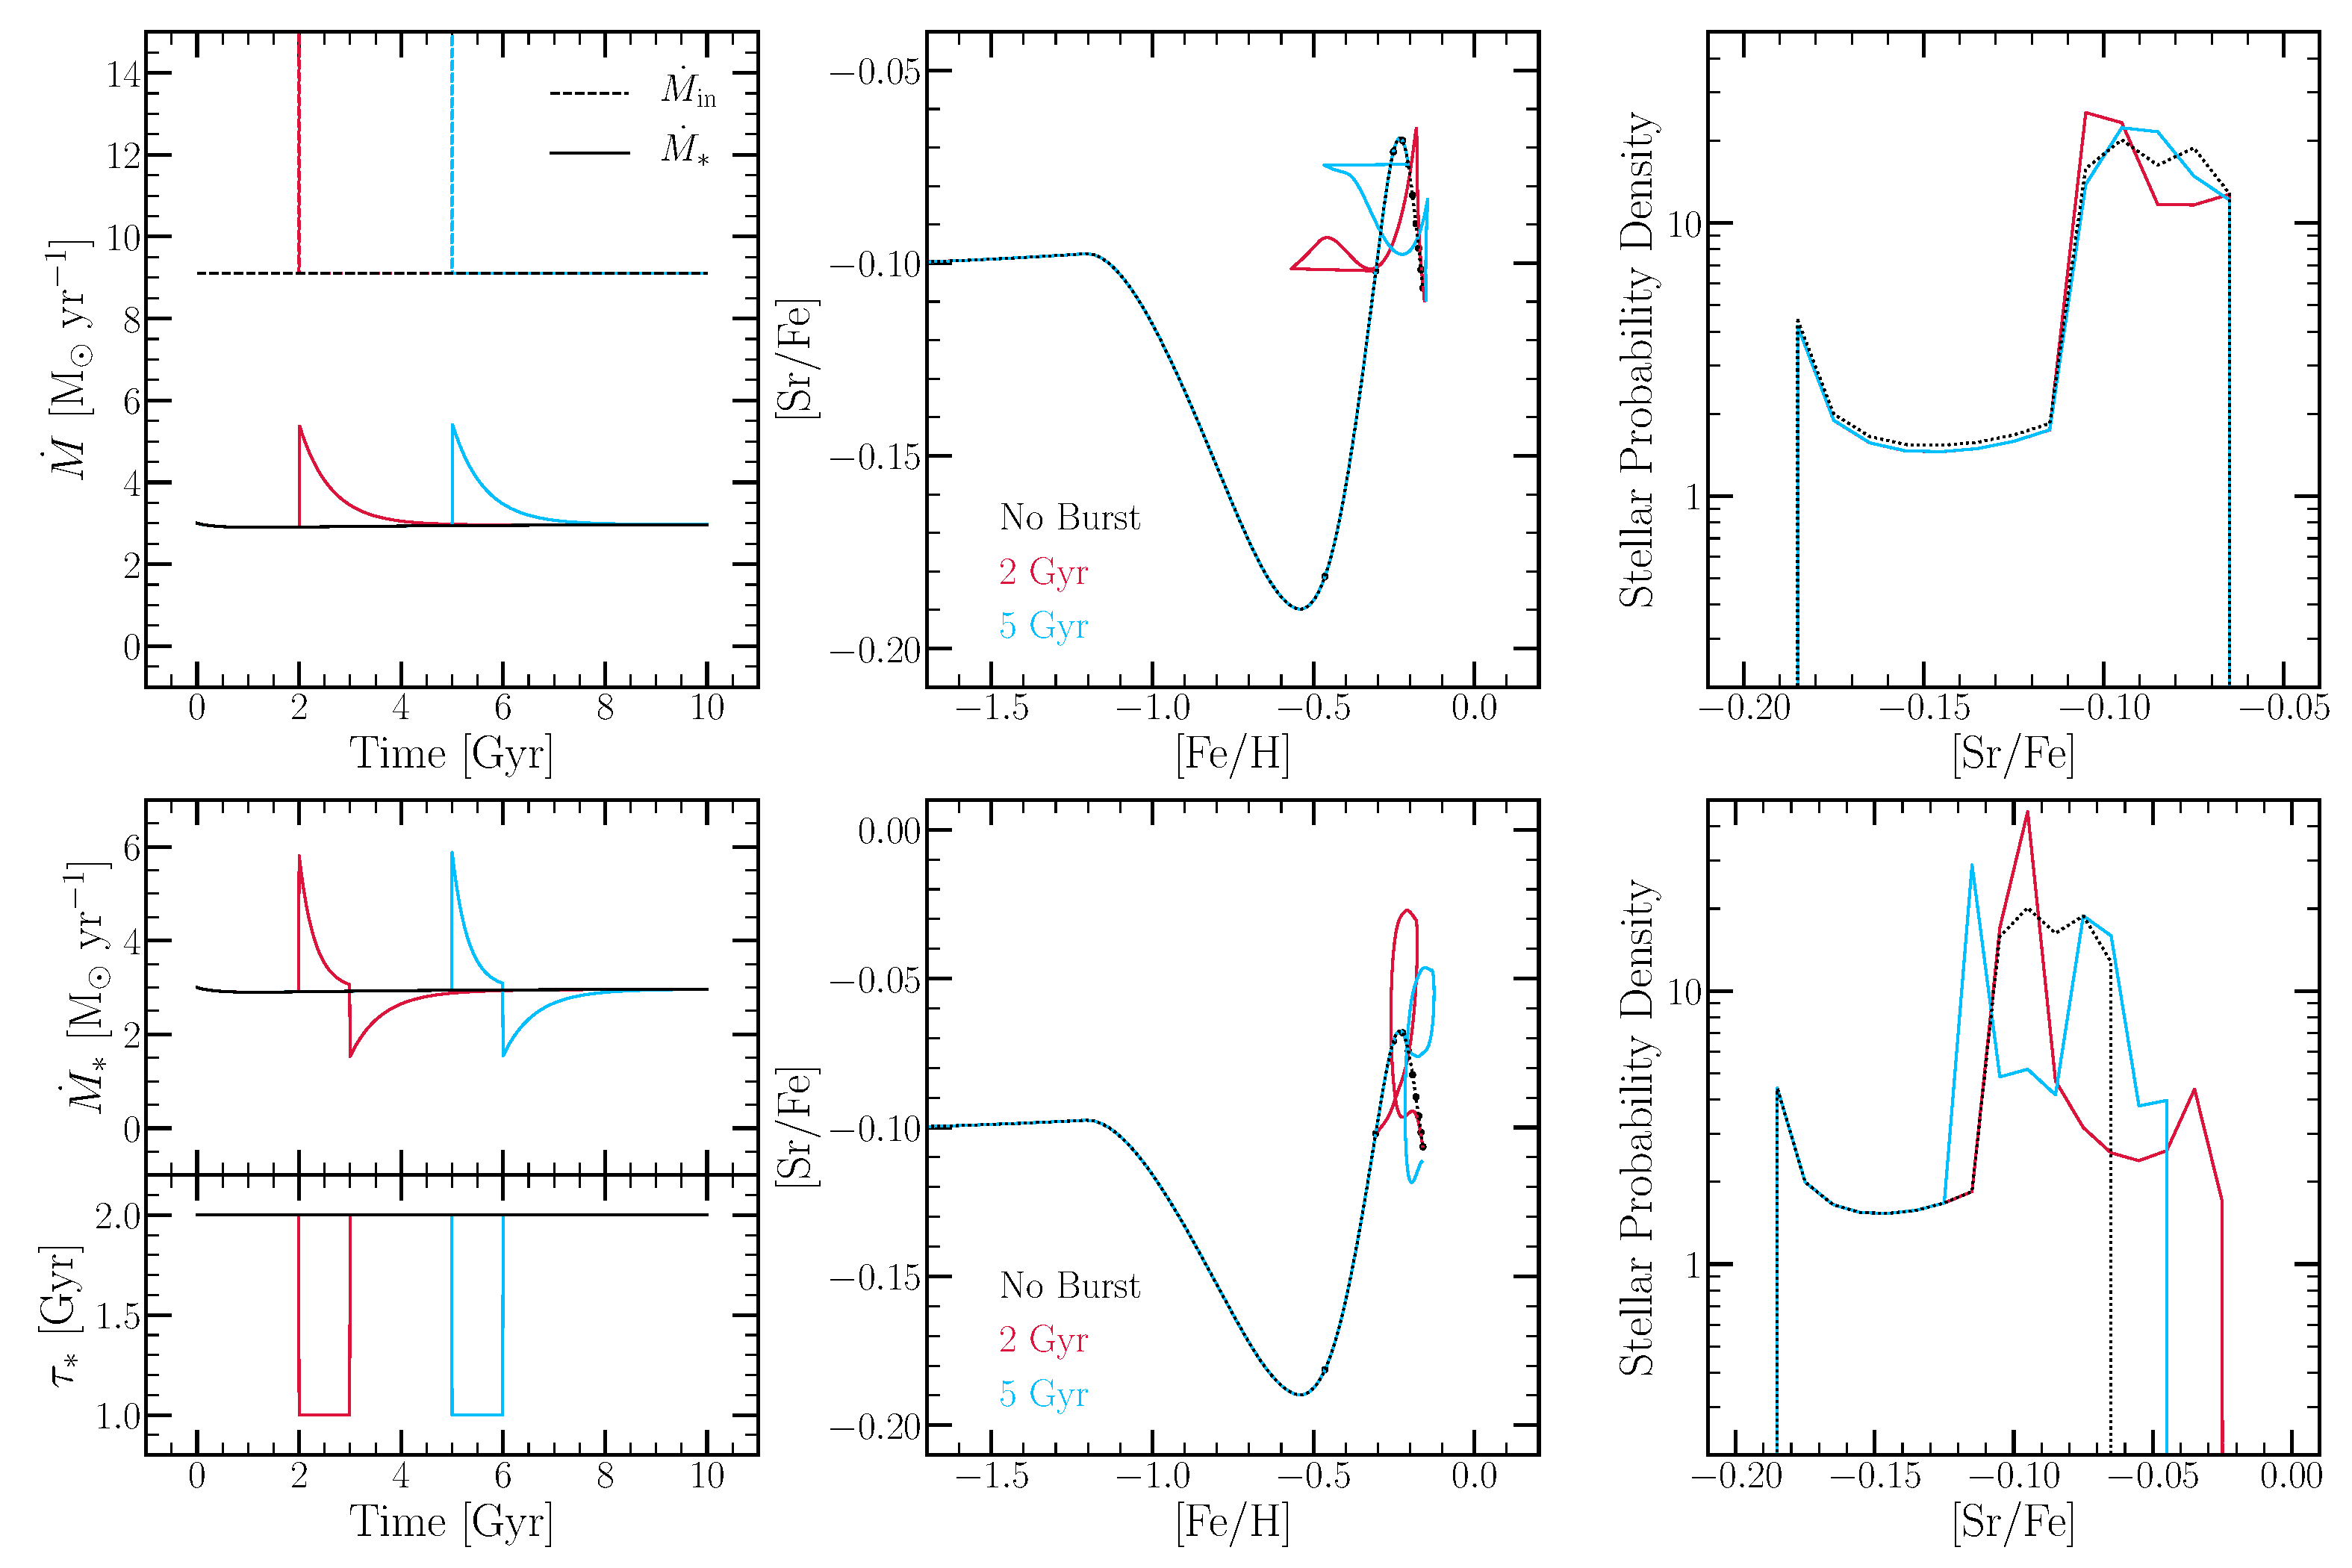
\includegraphics[scale = 0.31]{fiducial_bursts_sr.pdf}
\caption{
Evolutionary tracks (middle) and final [Sr/Fe] distributions (right) for our 
fiducial starburst models, analogous to the top and bottom rows of 
Fig.~\ref{bursts:fig:fiducial_cases}. All models adopt $y_\text{Sr}^\text{CC} = 
3.5\times10^{-8}$ and the~\citet{Cristallo2011} AGB yields illustrated in 
Fig.~\ref{bursts:fig:sryields_3panel}. 
}
\label{bursts:fig:bursts_srfe}
\end{figure*}

\subsection{Smooth Evolution}
\label{bursts:sec:sr_enrich} 

Fig.~\ref{bursts:fig:sr_yields} shows the [Sr/Fe]-[Fe/H] tracks and [Sr/Fe] 
distributions for our fiducial unperturbed GCE model, with constant SFR, 
$\tau_* = 2$ Gyr,~$\eta = 2.5$, and the AGB Sr yields illustrated in 
Fig.~\ref{bursts:fig:sryields_3panel}. We consider four different assumptions about 
CCSN yields: $y_\text{Sr}^\text{CC} = 0$, $y_\text{Sr}^\text{CC} = 
3.5\times10^{-8}$, and the metallicity dependent yields of 
equations~\refp{bursts:eq:y_sr_cc_linear} and~\refp{bursts:eq:y_sr_cc_limexp}. The 
$y_\text{Sr}^\text{CC} = 3.5\times10^{-8}$ model has a flat plateau at 
[Sr/Fe] = -0.1 for [Fe/H] $< -1.0$, which reflects the ratio of our constant 
CCSN yields. The [Sr/Fe] ratio then dips downward as SN Ia Fe enrichment 
becomes important, analogous to the knee in [O/Fe]-[Fe/H] evolution. However, 
as [Fe/H] rises further, AGB enrichment becomes competitive with CCSN 
enrichment, and [Sr/Fe] moves upward. After reaching a maximum at [Fe/H] = 
-0.2, [Sr/Fe] = -0.1, the [Sr/Fe] curves turns downward again because the 
timescale of SN Ia enrichment is longer than that of AGB enrichment. Even 
though single stellar populations generally produce Sr before Fe (see 
Fig.~\ref{bursts:fig:sryields_3panel}), the bulk of the Sr production in GCE follows 
the bulk production of more abundant elements like O and Fe due to the 
metallicity dependence of the yields. The [Sr/Fe] distribution of this model 
has a peak at [Sr/Fe]$\approx$-0.18, corresponding to the minimum in the 
[Sr/Fe]-[Fe/H] curve, and a second, higher peak at [Sr/Fe]$\approx$-0.1. In 
detail, this second peak is split in two, corresponding to the maximum in the 
[Sr/Fe]-[Fe/H] track and the slightly lower final equilibrium. 
\par 
With $y_\text{Sr}^\text{CC} = 0$ (AGB only), the [Sr/Fe] ratio is below -2 for 
[Fe/H] $<$ -1 and rises steeply with increasing [Fe/H], reaching a maximum at 
[Sr/Fe]$\approx$-0.35. Adding CCSN enrichment with $y_\text{Sr}^\text{CC} 
\propto Z$, corresponding approximately to the non-rotating~\citet{Limongi2018} 
yields, gives a shallower but still steeply rising [Sr/Fe]-[Fe/H] trend, which 
peaks at [Sr/Fe]$\approx$-0.1. Although one can see the imprint of SN Ia Fe 
enrichment on both of these curves, it is subtle relative to the strong trend 
arising from metallicity-dependent CCSN yields. 
\par 
Our approximate model of the rotating~\citet{Limongi2018} yields given by 
equation~\refp{bursts:eq:y_sr_cc_limexp} produces a [Sr/Fe] curve that rises rapidly 
until [Fe/H] = -1, then stays nearly constant at [Sr/Fe]$\approx$+0.2. AGB 
enrichment is small relative to CCSN enrichment in this model, as shown in 
Fig.~\ref{bursts:fig:sryields_3panel}. There is still a slight dip in [Sr/Fe] at 
late times, producing a split in the [Sr/Fe] distribution. 
\par 
Spectra of early-type galaxies imply [Sr/Fe]$\approx$0 for stellar populations 
typically dominated by solar or mildly super-solar 
metallicities~\citep{Conroy2013a}, showing that solar abundance ratios arise 
even in systems with very different star formation histories from the Milky 
Way. Measurements of individual stars in the Milky Way and in dwarf satellites 
show median trends that are roughly flat at [Sr/Fe]$\approx$0 down to 
[Fe/H]$\approx$-3, though the star-to-star scatter becomes large below 
[Fe/H] = -1~\citep[see, e.g.,][and references therein]{Mishenina2019, 
Hirai2019}. Above [Fe/H] = -1, our model with the~\citet{Limongi2018} rotating 
CCSN progenitor yields produces a flat [Sr/Fe] trend, but only our 
$y_\text{Sr}^\text{CC}$ = constant model produces a flat trend to [Fe/H] as low 
as -3. We conclude that reproducing Milky Way observations requires an 
additional source of Sr that is prompt compared to SN Ia enrichment and 
approximately independent of metallicity at least for [Fe/H] $< -1$. This is 
in agreement with more detailed models of Sr enrichment investigating a 
variety of potential sources, such as neutron star mergers, electron-capture 
and magnetorotationally driven supernovae, and rotating massive 
stars~\citep[e.g.][]{Cescutti2014, Cescutti2015, Prantzos2018, Hirai2019, 
Rizzuti2019}. Neutron-rich neutrino-driven winds from newly 
formed neutron stars should also produce Sr via r-process nucleosynthesis in 
core collapse supernovae~\citep{Thompson2001,Vlasov2017,Thompson2018}, and 
this production is typically not included in calculations of CCSN yields such 
as~\citet{Limongi2018}. Sources that produce relatively large amounts of Sr in 
events that are individually rare would help to explain the large star-to-star 
scatter at low [Fe/H]. We conclude that our constant $y_\text{Sr}^\text{CC} = 
3.5\times10^{-8}$ model could retroactively account for this contribution; 
this arises from the nature of equation~\refp{bursts:eq:mdot_ccsne} which in principle 
could fold all prompt enrichment components into $y_\text{Sr}^\text{CC}$ as a 
function of metallicity. Nonetheless, we encourage caution that sufficiently 
accurate modeling of Sr production at metallicities as low as [Fe/H] $< -2$ 
may require a more complete understanding of the astrophysical origins of the 
r-process and the associated Sr yields. 



\subsection{Burst Scenarios}

Fig.~\ref{bursts:fig:bursts_srfe} shows [Sr/Fe] evolution and [Sr/Fe] distributions 
for our fiducial gas-driven and efficiency-driven starbursts, which can be 
compared to the [O/Fe] result in the top and bottom rows of 
Fig.~\ref{bursts:fig:fiducial_cases}. For ease of interpretation we have used the 
$y_\text{Sr}^\text{CC} = 3.5\times10^{-8}$ model for CCSN yields, and the 
black curves representing the unperturbed model are the same as the black 
curves in Fig.~\ref{bursts:fig:sr_yields} but shown with a zoomed-in axis range. 
In the gas-driven models, dilution with pristine gas first drives [Fe/H] lower 
at fixed [Sr/Fe]. For the burst at $t = 2$ Gyr, this backward jump is followed 
by a small upward hook, reminiscent of the behaviour of this model in [O/Fe]. 
However, this burst occurs very near the [Sr/Fe] ratio associated with the 
adopted CCSN yields, suggesting that CCSNe associated with the burst do not 
significantly modify the ISM [Sr/Fe]. Instead, it is likely that this increase 
is due to Sr production in AGB stars from earlier epochs. Subsequently, the 
detailed shape of the trajectory becomes complex as both SN Ia and AGB 
enrichment with metallicity dependent yields become important, and eventually 
it rejoins the trajectory of the unperturbed model. 
\par 
The $t = 5$ Gyr burst occurs after the maximum [Sr/Fe], produced because a 
$t^{-1.1}$ SN Ia DTD produces Fe on timescales longer than AGB stars produce 
Sr. In this model, [Sr/Fe] initially evolves downward following the addition 
of zero metallicity gas, both because of these late SNe Ia from previous 
generations of stars and because this is in the direction of the CCSN ratio of 
[Sr/Fe]$\approx$-0.1. Unfortunately, all of these excursions are small, and 
the impact on [Sr/Fe] distributions is almost negligible. Detecting the 
signature of these complex tracks would require correlating precise [Sr/Fe] 
and stellar age measurements. 
\par 
The impact of efficiency-driven bursts (lower panels) is somewhat stronger. 
Here the bursts drive upward excursions in [Sr/Fe] because both the CCSN and 
AGB channels contribute Sr faster than SN Ia Fe, and the slight boost of [Fe/H] 
increases the AGB yield. As seen previously in [O/Fe], the suppressed SFR after 
$\tau_*$ returns to its original value causes a downward hook in [Sr/Fe], as 
SN Ia Fe from stars produced during the burst dominates over the reduced CCSN 
and AGB contributions. These models produce larger deviations in the [Sr/Fe] 
distributions than the gas-driven models, with peaks at higher and lower 
[Sr/Fe] associated with the mid-burst maximum and post-burst minimum. However, 
the separation between these peaks is below 0.1-dex, so precise measurements 
would be needed to detect this signature. 
\par 
The interpretation of Fig.~\ref{bursts:fig:bursts_srfe} is complicated partly by the 
fact that three enrichment processes are involved: CCSN, SN Ia, and AGB. 
Fig.~\ref{bursts:fig:sro_bursts} examines trajectories of [Sr/O] vs. [O/H], which are 
independent of SN Ia, at least given our assumption that SN Ia yields of O and 
Sr are insignificant. Here we show trajectories for our two 
metallicity-dependent CCSN yield models as well as the constant yield model. 
Tracks with smooth star formation (left panel) resemble the [Sr/Fe]-[Fe/H] 
tracks in Fig.~\ref{bursts:fig:sr_yields}, but without the dips coming for SN Ia Fe. 
For a gas-driven burst at $t = 5$ Gyr (middle panel), trajectories jump to 
lower [O/H] through dilution, then loop downward because the burst initially 
raises the rate of CCSN relative to AGB enrichment. These loops are analogous 
to the upward loops of [O/Fe], but O is now in the ratio denominator, and 
the timescales are CCSN vs. AGB rather than CCSN vs. SN Ia. The loop is flatter 
for the rotating star yield model because AGB stars make a smaller fractional 
contribution to Sr enrichment, and the CCSN contribution is boosted for both 
Sr and O during the burst. All trajectories eventually return to the late-time 
equilibrium of the unperturbed model. 
\par 
For an efficiency-driven burst at $t = 5$ Gyr (right panel), evolutionary 
tracks have a ``balloon-on-string'' appearance that can be understood as 
follows. By the time of the burst, the oxygen abundance has evolved to 
equilibrium, with 
\begin{equation} 
\label{bursts:eq:mdot_o_eq} 
\dot{M}_\text{O} \approx y_\text{O}^\text{CC}\dot{M}_* - 
(1 + \eta - r_\text{inst})\dot{M}_*(M_\text{O}/M_\text{ISM}) = 0 
\end{equation} 
where $M_\text{O}$ and $M_\text{ISM}$ are the oxygen and total mass in the ISM, 
respectively, and the oxygen abundance is 
\begin{equation} 
Z_\text{O,eq} = \left(\frac{M_\text{O}}{M_\text{ISM}}\right)_\text{eq} = 
\frac{y_\text{O}^\text{CC}}{1 + \eta - r_\text{inst}} 
\end{equation} 
\citep[][equations (11) and (14)]{Weinberg2017b}. Boosting the star 
formation efficiency does not initially perturb $\dot{M}_\text{O}$ from 
zero because the sources and sinks are both proportional to $\dot{M}_*$, but 
the ISM gas mass decreases because of more rapid consumption, so 
$Z_\text{O} = M_\text{O}/M_\text{ISM}$ rises. The [Sr/O] ratio drops slightly 
at first because CCSN enrichment has increased relative to AGB enrichment, but 
the increased metallicity boosts the AGB Sr yield, so [Sr/O] loops upward once 
AGB enrichment from the starburst becomes important. As the burst evolves 
further, sinks exceed sources in equation~\refp{bursts:eq:mdot_o_eq}, so the [O/H] 
ratio evolves backward to lower values because $Z_\text{O} > Z_\text{O,eq}$. 
This evolution ``overshoots'' the original [O/H] equilibrium as the gas supply 
evolves back to its original value. Lower metallicity in turn leads to a drop 
in Sr yields and [Sr/O]. Eventually all models evolve back to the original 
pre-burst equilibrium. The loop of the $y_\text{Sr}^\text{CC} \propto Z$ model 
is widest in the [Sr/O] dimension because for this model AGB and CCSN yields 
both change with metallicity, and CCSN enrichment dominates over AGB enrichment 
in the $y_\text{Sr}^\text{CC} \propto 1 - e^{-kZ}$ model. 
\par 
Figs.~\ref{bursts:fig:bursts_srfe} and~\ref{bursts:fig:sro_bursts} show that the evolution of 
an AGB s-process element can be intricate because of both the intermediate 
timescale of AGB enrichment and metallicity dependent yields. Unfortunately the 
perturbations of [Sr/Fe] and [Sr/O] ratios are relatively small, so diagnosing 
starbursts with these ratios will require precise abundance measurements 
and reasonably precise stellar ages. 



\section{Long Term Modulation of Star Formation Rates}
\label{bursts:sec:oscillatory} 

\begin{figure*} % fig 8
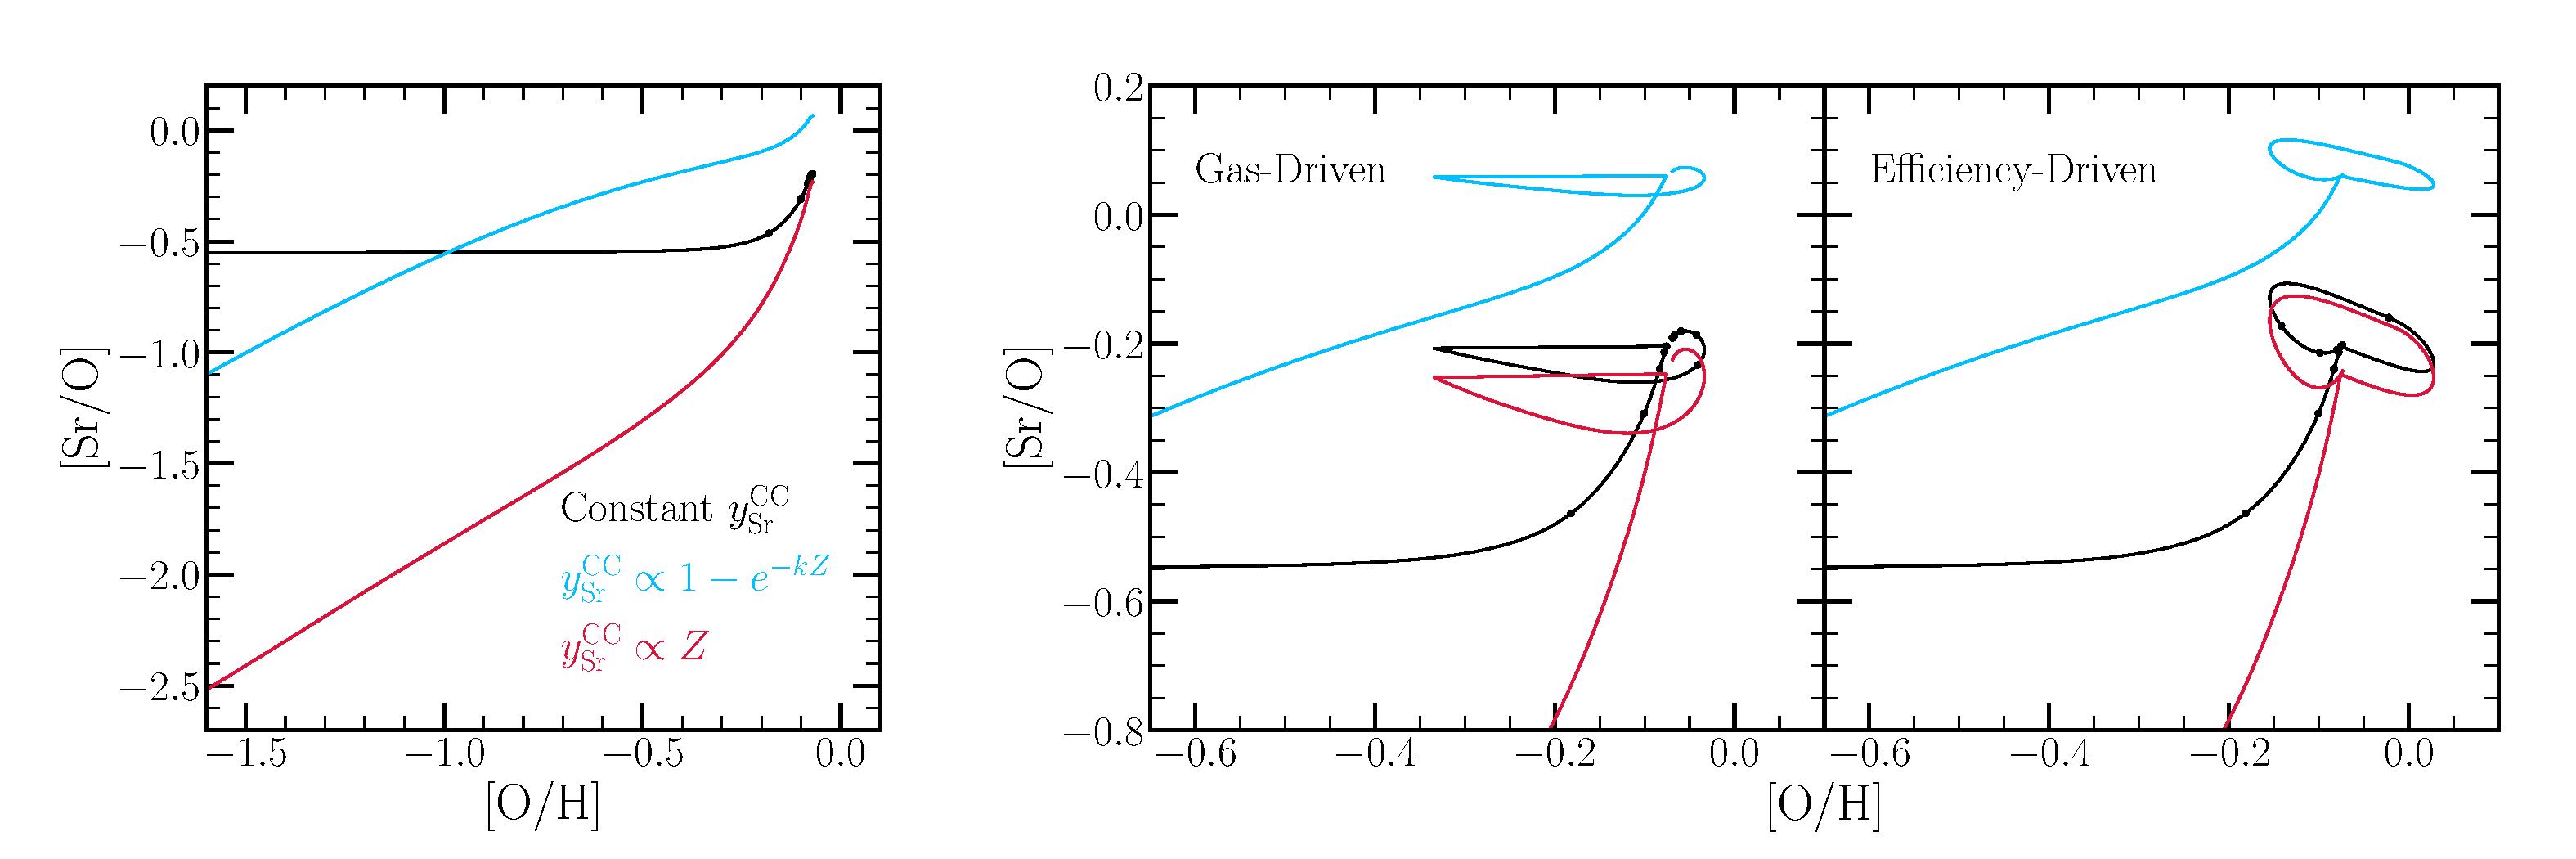
\includegraphics[scale = 0.32]{sro_bursts.pdf} 
\caption{
Evolutionary tracks in the [Sr/O]-[O/H] plane for our fiducial burstless 
model (left) and for our fiducial gas-driven (middle) or efficiency-driven 
(right) starburst models, for three models of the $y_\text{Sr}^\text{CC}$ yield 
as labeled. In contrast to Figs.~\ref{bursts:fig:sr_yields} and~\ref{bursts:fig:bursts_srfe}, 
these results are independent of SN Ia enrichment, simplifying interpretation. 
In the middle panels, tracks initially evolve to lower [O/H] because of gas 
dilution, while in the right panel they evolve to higher [O/H] because 
increased SFE reduces the gas supply. The [Sr/O] evolution is driven mainly by 
the metallicity dependence of the Sr yields. In all panels, 
points are plotted at 1-Gyr intervals on models shown in black. 
}
\label{bursts:fig:sro_bursts} 
\end{figure*} 

\begin{figure*} % fig 9
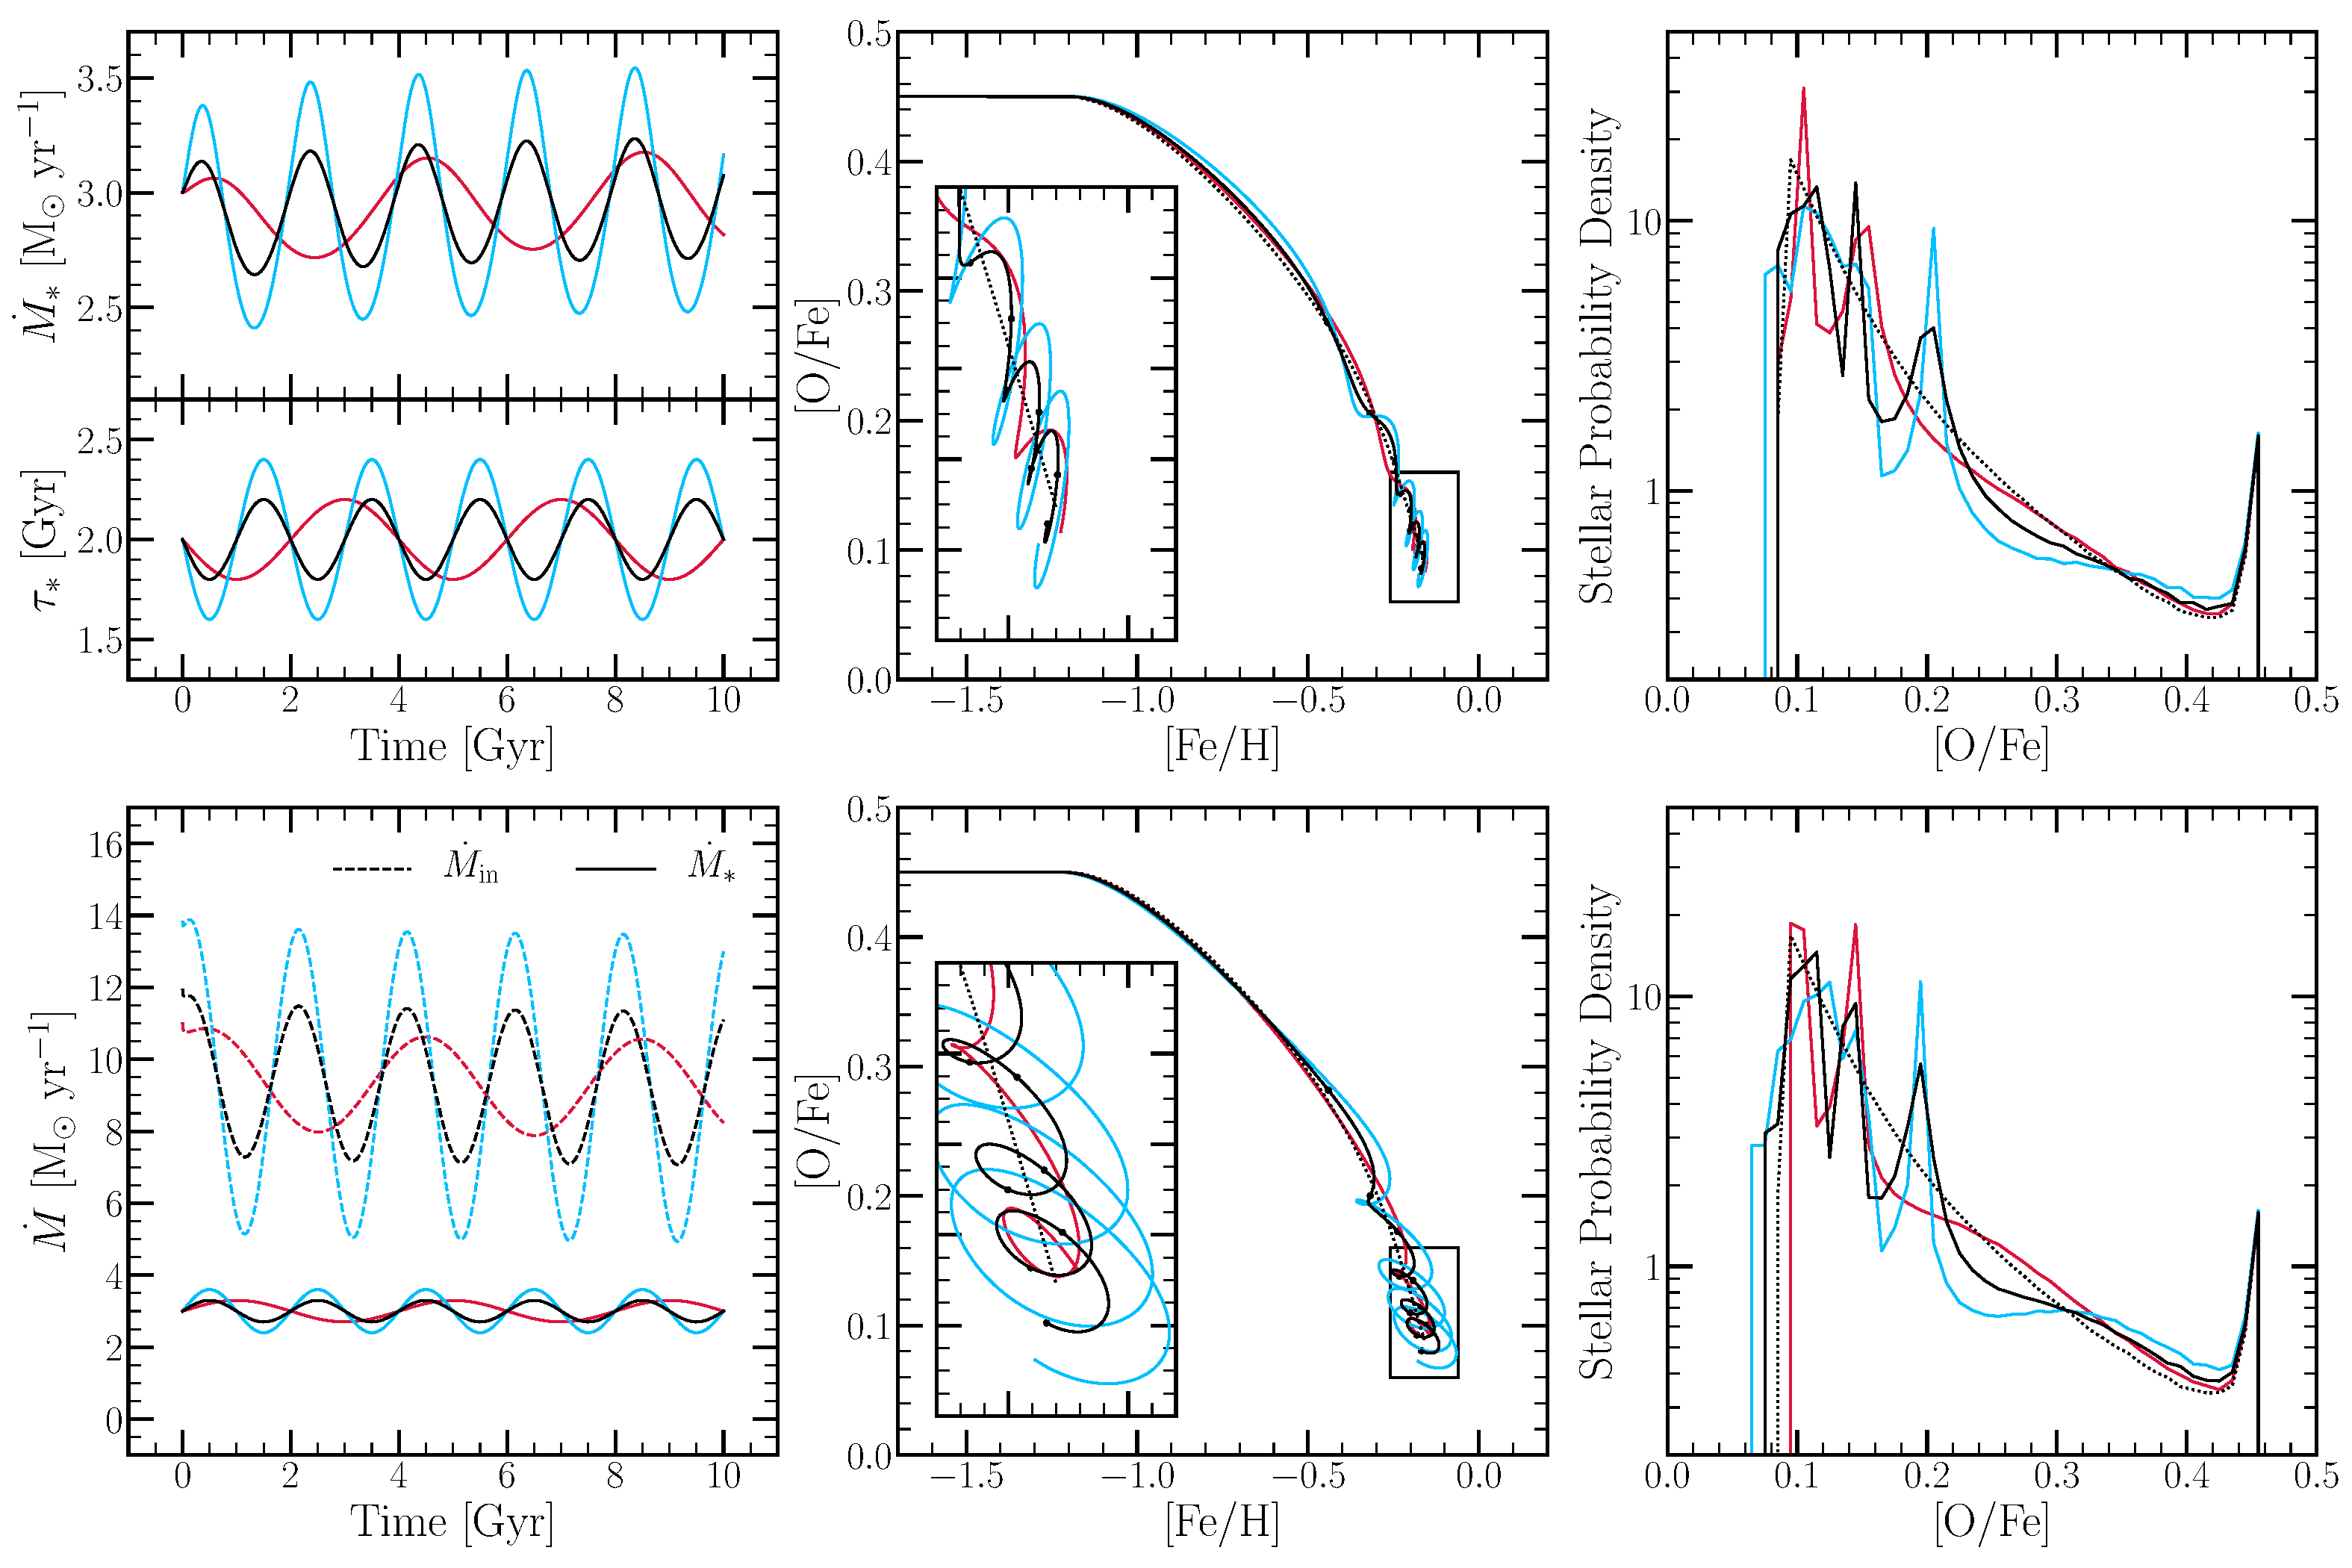
\includegraphics[scale = 0.32]{oscil.pdf} 
\caption{
Models with sinusoidal modulations of the SFR induced by modulations of the 
SFE timescale $\tau_*$ (top) or the gas infall rate $\dot{M}_\text{in}$ 
(bottom). Black curves represent a model with 10\% SFR modulations and a 2 Gyr 
period, while blue and red curves show the effect of doubling the amplitude or 
period of the modulation, respectively. In the middle and right panels, dotted 
black curves show results for our fiducial unperturbed model for comparison. 
In the middle panels, points are plotted at 1-Gyr intervals for the 10\% 
amplitude, 2-Gyr period model.
} 
\label{bursts:fig:oscil} 
\end{figure*} 

\begin{figure*} % fig 10 
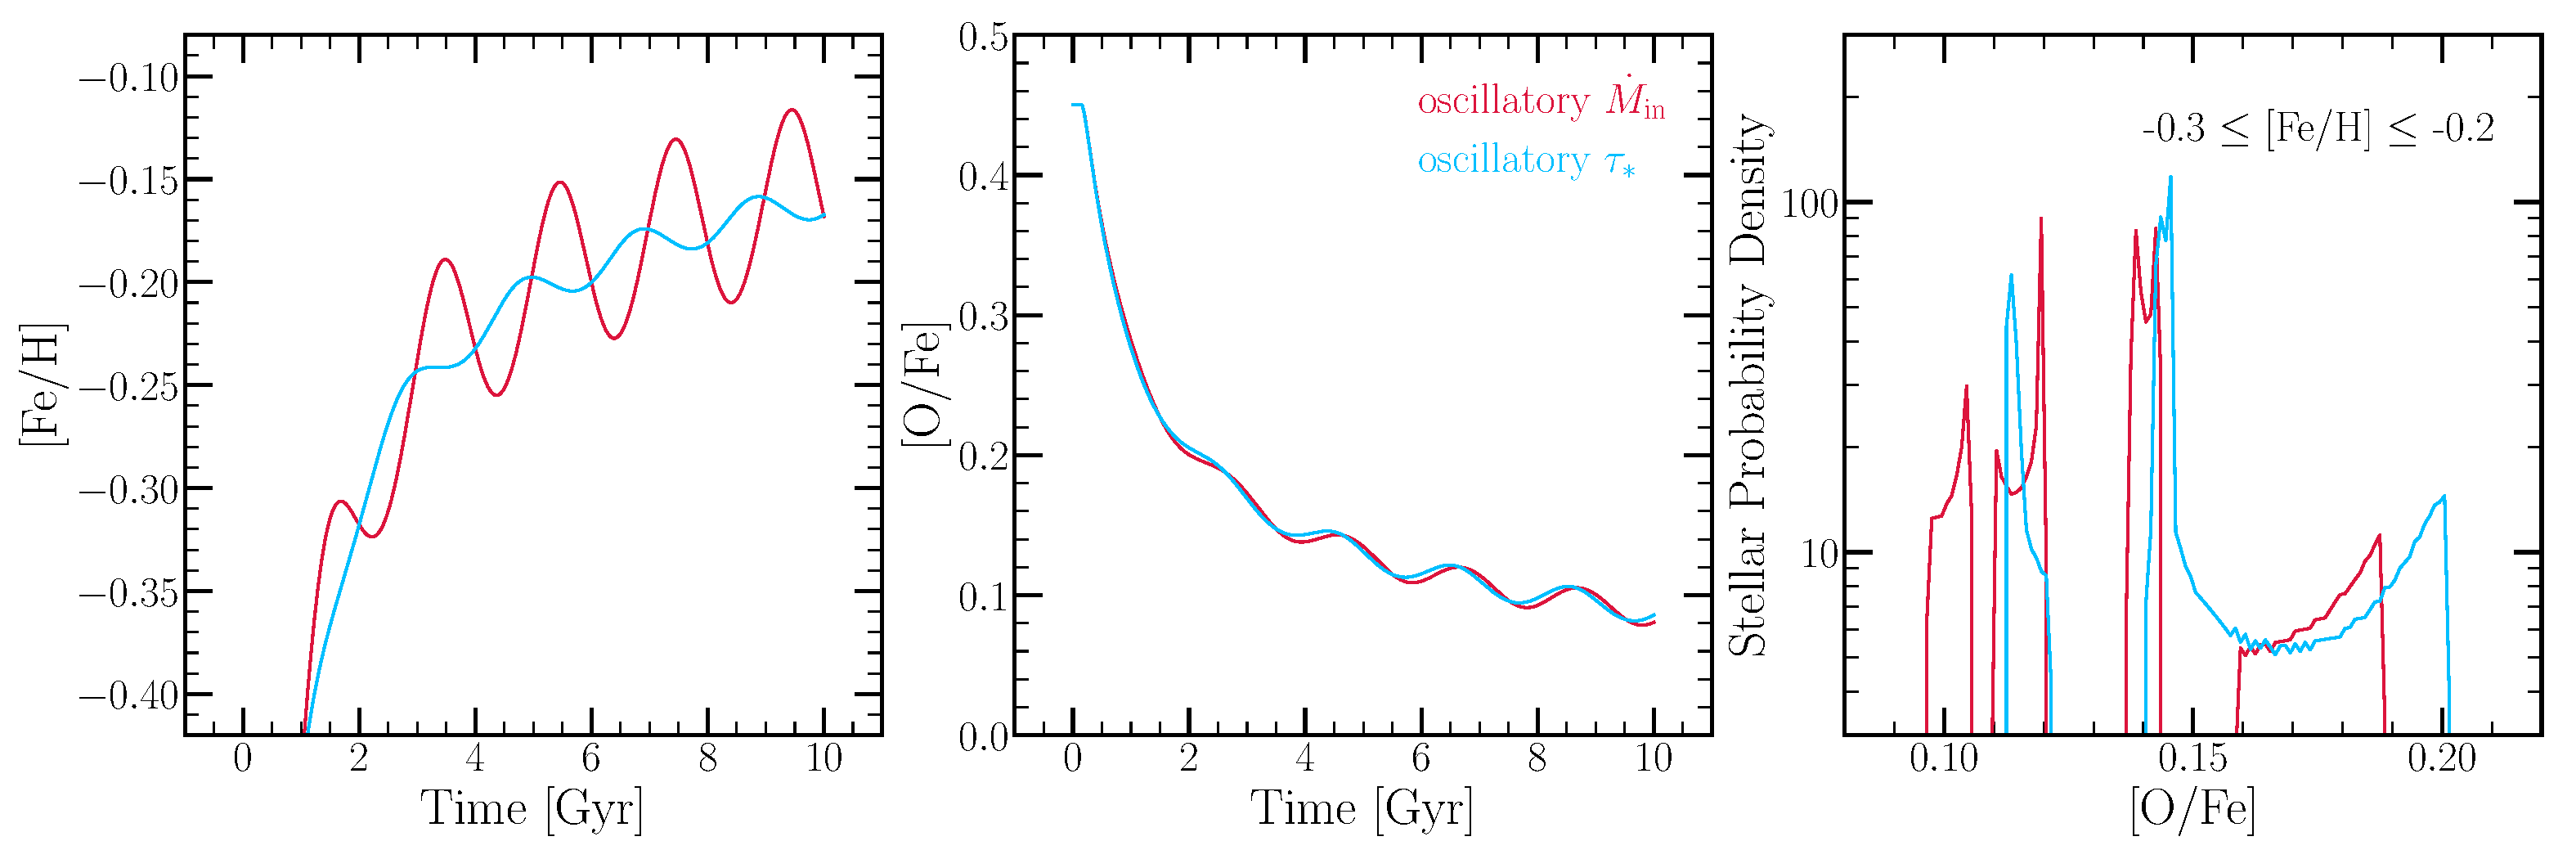
\includegraphics[scale = 0.32]{oscillations_v_time.pdf} 
\caption{
Time evolution of [Fe/H] (left) and [O/Fe] (middle) for the 20\% amplitude, 2 
Gyr models driven by $\tau_*$ modulations (red curves) or $\dot{M}_\text{in}$ 
modulations (blue curves). Oscillations of [Fe/H] are larger in the infall 
modulation model, but oscillations of [O/Fe] are similar in the two models. 
The right hand panel shows the [O/Fe] distributions for stars in the range 
-0.2$\leq$[Fe/H]$\leq$-0.3, demonstrating that at constant [Fe/H], the 
resultant [O/Fe] distribution is not a simple bimodal gaussian. 
} 
\label{bursts:fig:oscil_v_time} 
\end{figure*}

Bursts of star formation change the ratio of CCSNe to SNe Ia, producing loops 
in [O/Fe]-[Fe/H] trajectories and multiple peaks in [O/Fe] distributions. 
Slower, continuous variations of SFR also perturb the CCSN/SN Ia ratio in ways 
that can add complexity to these trajectories and distributions. From the 
standpoint of starbursts, such variations can be thought of as emulating a 
series of minor bursts throughout a galaxy's history, and are a possible 
source of scatter in [O/Fe] at fixed [Fe/H] in observed stellar populations. 
In the Milky Way disk,~\citet{BertranDeLis2016} estimate the intrinsic scatter 
in [O/Fe] as 0.03-0.04 dex in both the high-$\alpha$ (``chemical thick disk'') 
and low-$\alpha$ (``chemical thin disk'') stellar populations. 
\par
Fig.~\ref{bursts:fig:oscil} shows evolutionary tracks and [O/Fe] distributions for 
models with sinusoidal perturbations in SFR relative to a constant SFR model. 
In the upper panels, we create the SFR variations by modulating the SFE 
timescale $\tau_*$ about its baseline value of 2 Gyr. The black curve shows a 
model in which the amplitude of modulation is 10\% (i.e. 0.2 Gyr) and the 
period of modulation is 2 Gyr. Blue and red curves show models with a 20\% 
amplitude and a 4 Gyr period, respectively. The gas infall rate 
$\dot{M}_\text{in}$ and the outflow efficiency $\eta$ are held constant at 
their fiducial values. 
\par 
As one might expect from our efficiency-driven starburst models, each 
oscillation in $\tau_*$ induces a low amplitude loop in the [O/Fe]-[Fe/H] 
trajectory. For a 2 Gyr period, the first minimum in SFR occurs when [Fe/H] 
$\approx$ -0.45, and at lower metallicties the trjectory is only slightly 
different from that of an unperturbed model. At higher metallicities, there 
is a local maximum in [O/Fe] associated with each maximum in SFR, as one can 
see from the inset in the middle panel. The resulting [O/Fe] distributions 
have multiple peaks and troughs associated with flat and steep portions of the 
[O/Fe] trajectories, though these peaks can merge with each other into 
broader features. The peaks are sharper for higher amplitude modulations as 
expected. For the 10\% modulation, 2 Gyr period model there are three distinct 
peaks at [O/Fe] $\approx$ +0.11, +0.15, and +0.20, respectively, while the 
model with 4 Gyr period produces two distinct peaks at [O/Fe] $\approx$ +0.10 
and +0.15. 
\par 
The lower panels of Fig.~\ref{bursts:fig:oscil} show models in which we modulate 
the gas infall rate $\dot{M}_\text{in}$ while keeping $\tau_*$ and $\eta$ 
fixed. For these models we have chosen to modulate the \textit{star formation 
rate} $\dot{M}_*$ by 10\% or 20\% with a 2 or 4 Gyr period (solid curves in 
left panel). \texttt{VICE} automatically solves for the required modulations in 
$\dot{M}_\text{in}$ (dashed curves), which have the same period as the SFR 
modulations but a different phase and larger fractional amplitude. These gas 
supply modulations produce loops in [O/Fe] trajectories that resemble those of 
our infall-driven burst models. In particular, trajectories first move to lower 
[Fe/H] because of dilution, then to higher [O/Fe] and [Fe/H] because of 
subsequent star formation. The resulting [O/Fe] distributions show a multi-peak 
structure like that in the $\tau_*$-modulation models, with peaks at similar 
locations. 
\par 
Fig.~\ref{bursts:fig:oscil} shows that moderate amplitude fluctuations (10-20\%) of 
the SFR can produce a spread of [O/Fe] values at fixed [Fe/H], at 
the~$\sim$0.05-dex level. For $\tau_*$ modulations, this scatter appears 
mainly in the [O/Fe] dimension while for $\dot{M}_\text{in}$ modulations it 
appears in both the [O/Fe] and [Fe/H] dimensions, but the impact on the [O/Fe] 
distributions is similar. This is demonstrated further in the left and middle 
panels of Fig.~\ref{bursts:fig:oscil_v_time}, which compares the 20\% amplitude, 2-Gyr 
period models of the two modes of oscillations. The middle panel shows that 
both modes of oscillation produce strikingly similar evolution of the ISM 
[O/Fe] with time, but the oscillatory $\dot{M}_\text{in}$ model predicts much 
stronger oscillations in [Fe/H]. 
These results are in good agreement with the episodic SFH model for the 
Milky Way bulge in~\citet{Matteucci2019}, which shows qualitatively similar 
behavior in the [$\alpha$/Fe]-[Fe/H] plane. 
\par 
We also demonstrate in Fig.~\ref{bursts:fig:oscil_v_time} that these moderate 
variations do not produce a bimodal distribution in [O/Fe] at fixed [Fe/H] 
as observed in the Milky Way; a more dramatic departure from this class of 
models is required. The right panel shows the normalized stellar MDFs in [O/Fe] 
only considering stars with -0.3 $\leq$ [Fe/H] $\leq$ -0.2, and although these 
display complex structure, neither model reproduces the [O/Fe] distribution 
found by, e.g.,~\citet{BertranDeLis2016}, which is well described by two 
Gaussians separated by~$\sim$0.15 dex. It is also notable that these SFR 
modulations only induce scatter in [O/Fe] at locations well beyond the knee 
of the [O/Fe]-[Fe/H] track. In part this is because our chosen parameters 
predict models which evolve past the knee quickly, before a full cycle of the 
SFR modulation. However, enrichment near the [O/Fe] plateau is dominated by 
CCSN in any case, so fluctuations in the SFR that change the CCSN rate have 
little leverage on [O/Fe]. Explaining intrinsic scatter in [O/Fe] (or ratios 
for other $\alpha$-elements) near the plateau of the high-$\alpha$ sequence 
requires a different mechanism, such as incomplete mixing of CCSN ejecta that 
individually have varying [O/Fe] ratios. 



\section{Slow Starburst in the Milky Way} 
\label{bursts:sec:slowburst} 

\begin{figure*} % fig 11 
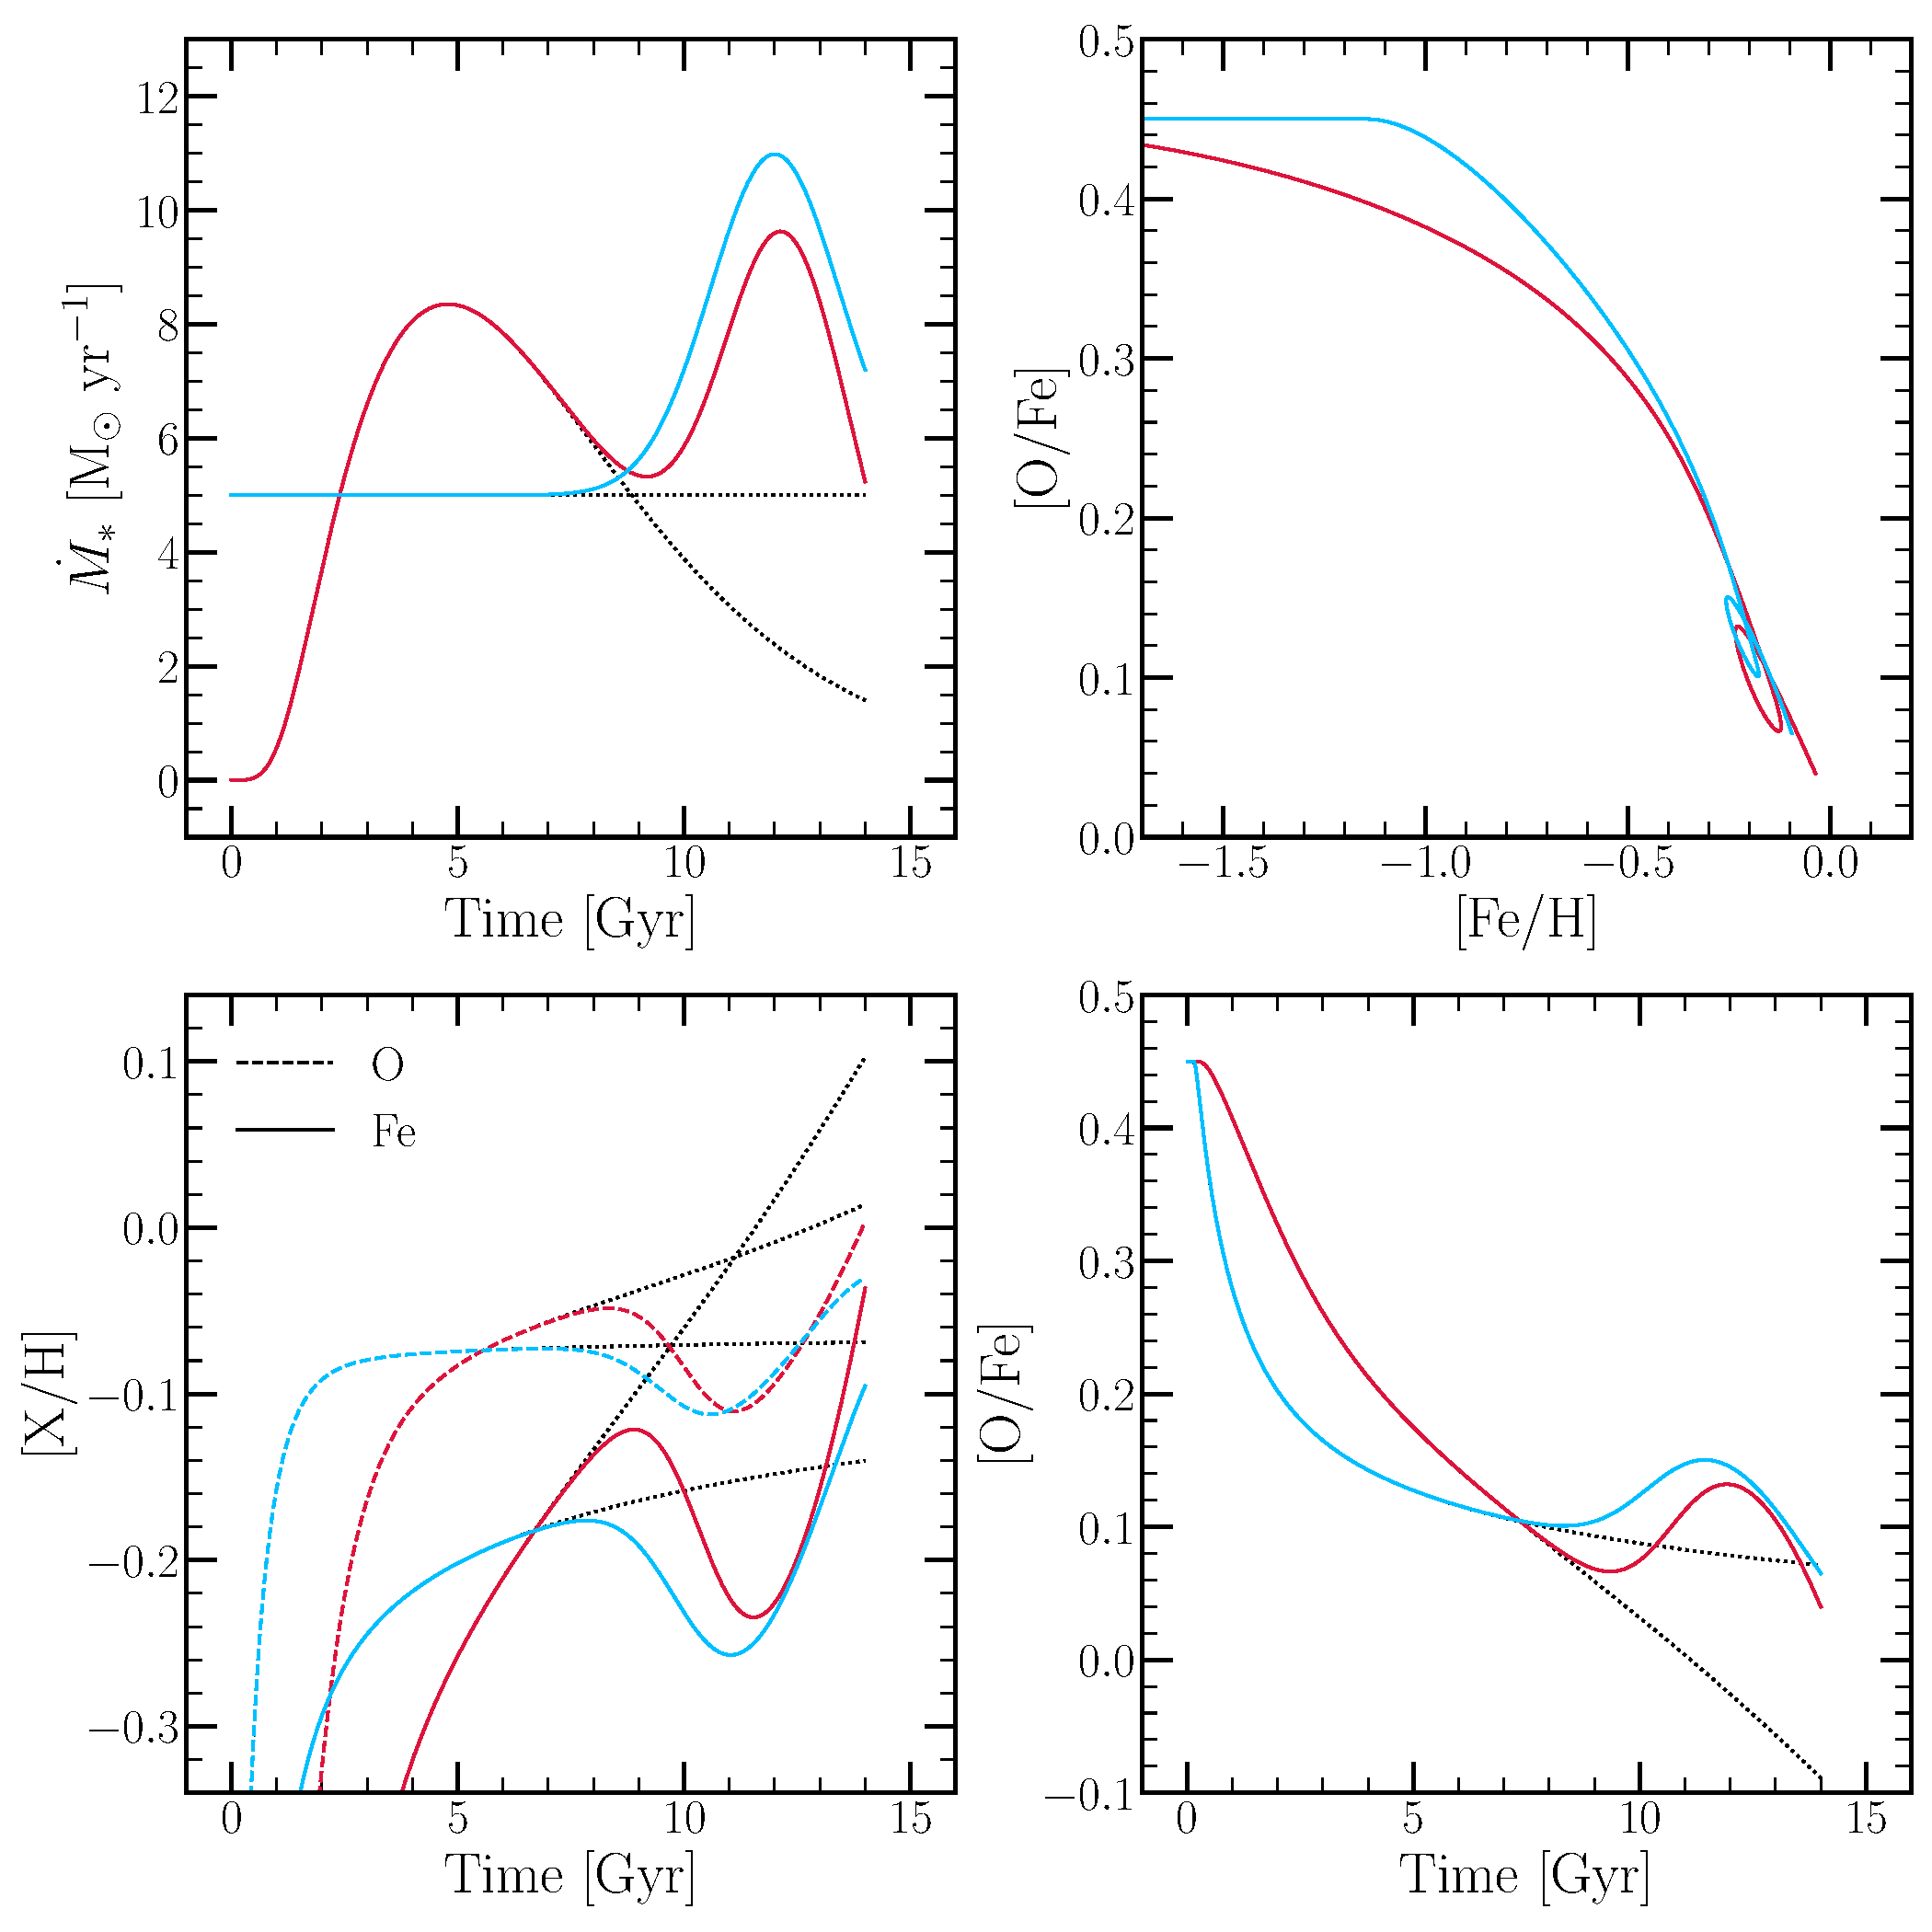
\includegraphics[scale = 0.4]{slow_bursts.pdf} 
\caption{
Models loosely motivated by recent findings of a slow starburst in the Milky 
Way~$\sim$2 Gyr ago~\citep{Mor2019, Isern2019}. These models exhibit a 
constant SFR (blue) and a $\propto t^2e^{-t}$ infall history (red), to which 
we add a Gaussian centered at $t$ = 12 Gyr with dispersion $\sigma$ = 1 Gyr to 
both models, roughly doubling the SFR at its peak. Black dotted lines in all 
panels show the corresponding quiescent scenario, to which we add no starburst. 
\textbf{Top Left}: The SFR as a function of time. 
\textbf{Top Right}: The [O/Fe]-[Fe/H] tracks. We omit the tracks of the 
quiescent model from this panel for clarity. 
\textbf{Bottom Left}: [O/H] (dashed) and [Fe/H] (solid) as a function of time. 
\textbf{Bottom Right}: [O/Fe] as a function of time. 
These models produce mildly $\alpha$-enhanced stars with young ages and a low 
median age of stars near solar metallicity. 
} 
\label{bursts:fig:slow_bursts} 
\end{figure*} 

Although our starburst models are most obviously relevant to dwarf galaxies 
with episodic star formation histories, some recent observations suggest that 
the Milky Way itself experienced substantially elevated star formation 2-3 Gyr 
ago. \citet{Mor2019} infer such a history by comparing population synthesis 
models to observed stellar luminosity functions and color-magnitude diagrams 
from Gaia data. \citet{Isern2019} reaches similar conclusions from modeling the 
luminosity function of white dwarfs in the solar neighborhood measured using 
Gaia parallaxes. Although these white dwarfs are close to the sun, dynamical 
mixing implies that they at least sample the history of the solar annulus, 
and older white dwarfs likely sample a range of galactocentric radii because of 
radial mixing. Resolved stellar population studies of the M31 disk also provide 
evidence for elevated star formation 2-4 Gyr ago with much lower SFR before 
and after~\citep[][Figs. 22-23]{Williams2017}. 
\par 
Fig.~\ref{bursts:fig:slow_bursts} presents the evolution of two models loosely 
motivated by these observations. The first (blue curves) has a constant SFR to 
which we have added a burst described by a Gaussian centered at $t = 12$ Gyr 
(lookback time 2 Gyr) with dispersion of 1 Gyr. At its peak, this burst 
approximately doubles the galaxy SFR relative to the pre-burst value. The 
second model (red curve) adds a similar burst to a model with an infall 
history described by $\dot{M}_\text{in} \propto t^2e^{-t}$ with $e$-folding 
timescale $\tau_\text{inf} = 2.2$ Gyr. The pre-burst SFR first climbs as the 
gas supply builds (starting from zero), then declines as the infall rate slows. 
The qualitative appearance of this model is similar to those in Fig. (1) 
of~\citet{Isern2019}. For both models we adopt $\eta$ = 2.5 and 
$\tau_* = (\text{2 Gyr})(M_\text{g}/6.0\times10^9\ M_\odot)^{-0.5}$, allowing 
\texttt{VICE} to solve for the infall rate required to produce the starburst. 
We also plot the evolution of the corresponding quiescent models in dotted 
lines for comparison; they follow the same evolution but with no added 
starburst. 
\par 
The [O/Fe]-[Fe/H] tracks show loops similar to those of our infall-driven and 
efficiency-driven burst models (e.g., Fig.~\ref{bursts:fig:fiducial_cases})
and qualitatively resemble that of~\citet{Spitoni2019}, who investigated 
similar models for the solar annulus in much greater detail. 
As found 
in previous studies~\citep{Andrews2017, Weinberg2017b}, the exponential 
infall model exhibits slower pre-burst evolution and a more gradual ``knee'', 
and because of the short $e$-folding timescale even the unperturbed model does 
not approach equilibrium by $t$ = 14 Gyr. The critical feature of these models 
relative to our fiducial starbursts is that the effects of the bursts have not 
decayed by the end of the simulations at $t$ = 14 Gyr. Over the final 2 Gyr, 
the values of [O/H] and [Fe/H] are rapidly climbing and end at values higher 
than those reached at any previous time. The [O/Fe] values in both models 
reach a local maximum at $t$ = 12 Gyr, then fall for the final 2 Gyr. 
\par
{\sloppy
These results are of particular interest in light of recent 
studies of age-abundance relations from the Apache Point Observatory Galaxy 
Evolution Experiment \linebreak \citep[APOGEE; e.g.,][]{Martig2016,
SilvaAguirre2018, Feuillet2018, Feuillet2019}.
}
The late bump in [O/Fe] could 
help explain populations of young $\alpha$-enhanced stars~\citep{Martig2016, 
Feuillet2019}, though in these models such stars would have modest 
$\alpha$-enhancements, 
near-solar metallicity, and age $\approx$ 2 Gyr. The late-time bumps in [O/H] 
and [Fe/H] could help to explain the strikingly young (1-2 Gyr) median ages that 
\citet{Feuillet2018} find for solar neighborhood stars with [Fe/H] $\approx$ 
0 or [O/H] $\approx$ 0. Finally, the most $\alpha$-poor stars predicted by 
these models form at late times in the wake of the burst, potentially 
explaining the low median age ($\sim$1 Gyr) that~\citet{Feuillet2018} find for 
stars with [$\alpha$/Fe] $<$ 0. The age-metallicity relation 
for solar neighborhood stars exhibits large scatter~\citep{Edvardsson1993}, 
and explaining this scatter likely requires radial mixing of stellar 
populations~\citep[e.g.][]{Schoenrich2009a} or some other mechanism not 
represented in one-zone GCE models. However, while multi-zone models with 
radial mixing and smooth star formation histories can explain a large 
dispersion in age-abundance relations, they still have difficulty reproducing 
the young median ages inferred for solar metallicity stars~\citep[][see 
their Fig. 15]{Feuillet2018}. 
The one-zone models presented here suggest that elevated star formation in the 
recent past could have a significant impact on age-abundance relations, 
pushing them away from the equilibrium behaviour predicted for smooth star 
formation histories. Furthermore, the differences between these models and 
their corresponding quiescent cases at late times raise the intriguing 
possibility that the recent burst in the Milky Way has not yet fully decayed. 
This would imply that the present day chemistry of the Milky Way is still 
mildly perturbed due to the recent starburst. We reserve an exploration of 
models combining radial mixing with star formation histories like those 
of~\citet{Mor2019} and~\citet{Isern2019} for future work.



\section{Conclusions}
\label{bursts:sec:conclusion} 

We have studied one-zone chemical evolution models tracking the enrichment of 
oxygen, iron, and strontium with the goal of understanding the impact of star 
formation bursts on elemental abundance ratios. To this end, we have developed 
the \texttt{Versatile Integrator for Chemical Evolution} (\texttt{VICE}), a 
\texttt{python} package optimized for handling highly non-linear chemical 
evolution models. With this new tool, we first simulated gas-driven 
starbursts, whereby an amount of gas comparable to the current ISM mass of a 
galaxy is added to the ISM on timescales shorter than the depletion time. 
These starburst models predict hooks in the [O/Fe]-[Fe/H] plane; the rapid 
addition of pristine gas first causes a reduction in [Fe/H] at fixed [O/Fe], 
then the elevated rate of CCSNe relative to SNe Ia drives the ISM to higher 
[O/Fe] and [Fe/H], and finally the onset of SNe Ia associated with the 
starburst pushes the ISM back toward the [O/Fe]-[Fe/H] track of the unperturbed 
(i.e. no-burst) model. The rate at which extra gas is added to the galaxy 
affects the detailed shape of these jump-and-hook trajectories. 
Although this paper focuses on characterizing model predictions
rather than interpreting data, we provide an illustrative comparison to
Kirby et al.'s (\citeyear{Kirby2010}) abundance measurements for 
Milky Way dwarf satellites in Appendix~A.
\par 
Our unperturbed constant-SFR models predict one peak in the [O/Fe] distribution 
at the ``plateau'' ratio of CCSN O and Fe yields, and a second peak associated 
with the late-time equilibrium in which CCSN and SN Ia rates are equal. Our 
gas-driven starburst models predict a third peak in the [O/Fe] distribution, 
associated with stars that form out of the $\alpha$-enhanced ISM 
during/following the burst before SNe Ia have driven evolution back toward the 
unperturbed evolutionary track. The peak is centred near the value of [O/Fe] 
at the top of the hook in the [O/Fe]-[Fe/H] trajectory, and its location and 
shape are insensitive to the timescale on which the gas is added, provided 
that this timescale is short compared to the depletion time. Earlier 
starbursts produce this third peak at higher [O/Fe] because they arise when 
the starting value of [O/Fe] is further from its eventual equilibrium. Thus, 
even without accurate ages for individual stars, the existence of extra 
peaks in the [O/Fe] distribution (or [X/Fe] distribution for other 
$\alpha$-elements) can provide an observable diagnostic for past bursts of 
galactic star formation, and the locations of these peaks can provide 
estimates of the timing of these bursts. 
\par 
A gas-driven starburst could arise from the merger of a gas rich system or a 
temporary increase in accretion rate. A starburst can also arise from a 
temporary increase in star formation efficiency, consuming the available gas 
more quickly, perhaps because of a dynamical disturbance that does not 
increase the gas supply. The evolutionary tracks of efficiency-driven 
starbursts differ in form from those of gas-driven starbursts, first because 
there is no drop in [Fe/H] before the increase in [O/Fe], and second because 
[O/Fe] loops below the track of the unperturbed model once the post-burst 
gas supply is depleted, which allows the CCSN rate to fall well below the rate 
of SNe Ia from stars that formed during the burst. With sufficiently precise 
data, the [O/Fe] distribution of an efficiency-driven burst can be 
distinguished from that of a gas-driven burst, in part by the shape of the 
[O/Fe] peak for $\alpha$-enhanced stars formed during the burst, and in part 
by the presence of an additional population of $\alpha$-deficient stars. 
\par 
In short, the chemical response to a simple starburst is driven by a 
perturbation of the CCSN and SN Ia rates. Conventionally, one-zone models tie 
the outflowing wind to the instantaneous star formation rate (i.e. 
$\dot{M}_\text{out} = \eta\dot{M}_*$), which in turn ties it to the CCSN rate. 
If SNe Ia contribute to the outflowing wind, then a better approximation of 
the outflow rate would be one that is tied to a time-averaged SFR (i.e. 
$\dot{M}_\text{out} = \eta\langle\dot{M}_*\rangle_{\tau_\text{s}}$), where 
$\tau_\text{s}$ is the outflow smoothing time. Nonzero $\tau_\text{s}$ allows 
the ISM to retain more gas at the onset of a starburst, because the outflow is 
more sensitive to the preburst SFR. The ISM is then gas-poor in the decay of 
the starburst, because the outflow is most sensitive to the elevated SFR from 
the recent burst. Varying $\tau_\text{s}$ between 0 and 1 Gyr has minimal 
impact on the predicted [O/Fe]-[Fe/H] trajectory or the stellar [O/Fe] 
distribution of gas-driven starbursts. However, efficiency-driven burst models 
with $\tau_\text{s}$ = 0.5 - 1 Gyr exhibit wider loops and produce lower 
[$\alpha$/Fe] stars than in the $\tau_\text{s}$ = 0 model. These 
$\alpha$-deficient stars are produced late in the burst when the ISM is 
gas-poor, an effect that is magnified by a nonzero $\tau_\text{s}$ because 
the gas outflow rate is higher and the CCSN rate is lower. 
\par 
While our simplest starburst scenarios are either gas- or efficiency-driven, 
there is observational evidence for starbursts driven by both 
an increase in the gas supply and an increase in the 
efficiency~\citep[][and the citations therein]{Kennicutt2012}. As a simple 
example of a ``hybrid'' starburst, we considered a model with a rapid influx 
of gas and an SFE timescale $\tau_* \propto M_\text{g}^{-1/2}$ as suggested 
by the Kennicutt-Schmidt law~\citep{Schmidt1959, Schmidt1963, Kennicutt1998}. 
For $\tau_\text{s}$ = 0 or 0.5 Gyr, the [O/Fe]-[Fe/H] tracks of this model are 
nearly the same as those of the gas-driven constant-$\tau_*$ model. For 
$\tau_\text{s}$ = 1 Gyr, the hybrid model shows aspects of both gas-driven and 
efficiency-driven models, including a population of $\alpha$-deficient stars. 
\par 
The AGB models of~\citet{Cristallo2011} predict Sr yields that are strongly 
dependent on metallicity and dominated by 2 - 4 $M_\odot$ stars. Predicted 
CCSN yields of Sr are sensitive to rotationally induced mixing; 
the~\citet{Limongi2018} yields for non-rotating progenitors vs. progenitors 
with $v_\text{rot}$ = 150 km s$^{-1}$ differ by 1-2 orders of magnitude, with 
strong but differing metallicity dependence. Near solar metallicity, the AGB 
yields and non-rotating CCSN yields are comparably important, but the 
$v_\text{rot}$ = 150 km s$^{-1}$ CCSN yields would outweight AGB yields by a 
large factor. 
\par 
Reproducing the approximately flat trend of [Sr/Fe] vs. [Fe/H] found in the 
Milky Way and in dwarf satellites~\citep{Mishenina2019, Hirai2019} requires 
an additional source of Sr with a yield that is nearly independent of 
metallicity, perhaps the neutrino-driven winds from newly formed neutron 
stars~\citep{Thompson2001, Vlasov2017, Thompson2018}. For any of these CCSN 
yield models, the tracks of [Sr/Fe] vs. [Fe/H] in starburst models are complex, 
affected by the yield metallicity dependence and by the differing timescales 
of CCSN, AGB, and SN Ia enrichment. Tracks of [Sr/O] vs. [O/H] are simpler 
because they are independent of SN Ia enrichment. However, the total range 
of [Sr/Fe] or [Sr/O] induced by starbursts is small, typically 0.05-0.1 dex, 
and in combination with yield uncertainties this small dynamic range makes it 
difficult to use Sr abundances as a diagnostic of starburst behavior. 
\par 
In addition to strong (factor of~$\sim$2) starbursts, we have investigated 
models with 10-20\% sinusoidal modulations of a constant SFR, induced by 
variations in infall rate or star-formation efficiency. These models predict 
[O/Fe]-[Fe/H] tracks that oscillate about the prediction of the constant SFR 
model. The produce a multi-peaked structure in [O/Fe] distributions, though 
in the presence of observational errors these peaks would likely merge into 
a broader distribution. These variations do not produce a bimodal [O/Fe] 
distribution, so they are not the origin of the observed separation of thin 
and thick disk sequences~\citep[e.g.][]{Bensby2003, Hayden2015, 
BertranDeLis2016}. However, moderate variations in SFR could be a source of 
scatter in [O/Fe] along these sequences. With our adopted parameter values, 
our smooth evolution models approximately reproduce the observed high-$\alpha$ 
sequence. SFR oscillations produce a spread of~$\sim$0.05-0.1 dex in [O/Fe] 
for [Fe/H] $\gtrsim$ -0.4, but they cannot produce scatter near the 
high-$\alpha$ plateau of this sequence because the enrichment of those stars 
is dominated by CCSN in any case. 
\par 
Motivated by findings on the recent star formation history of the 
Milky Way by~\citet{Mor2019} and~\citet{Isern2019}, we explored 
models that exhibit slow, factor of~$\sim$2 increases in the SFR at lookback 
times of~$\sim$2 Gyr, adopting a simple gaussian with dispersion of $\sigma$ = 
1 Gyr to describe the starburst. A late-time, slow starburst may help to 
explain otherwise puzzling features of the age-abundance relations observed 
in APOGEE~\citep{Martig2016,SilvaAguirre2018,Feuillet2018,Feuillet2019}, such 
as young stars with mild $\alpha$-enhancements and young median ages of solar 
metallicity or $\alpha$-deficient stars. Complete modeling of these 
observables requires multizone models that account for radial mixing of 
stellar populations, and we reserve such investigations to future work. 
\par 
Throughout this paper we have adopted an O yield similar to those predicted 
by~\citet{Chieffi2004} and~\citet{Chieffi2013}, assuming a Kroupa IMF in which 
all stars with $M > 8\ M_\odot$ explode. With this yield, evolving to solar 
metallicity requires fairly strong outflows, with $\eta$ = 2.5
\citep[e.g.,][]{Finlator2008, Peeples2011, Andrews2017, Weinberg2017b}.
% (e.g.,~\citealp{Finlator2008};~\citealp{Peeples2011};~\citetalias{Andrews2017}; 
% \citetalias{Weinberg2017}).
With lower IMF-averaged SN yields, which could 
arise if many massive stars form black holes instead of exploding, lower 
values of $\eta$ would be needed to reach the same final metallicity.  
Results for lower yield, lower $\eta$ models would differ in detail from those 
presented here, mainly because the depletion time $\tau_\text{dep} = 
\tau_*/(1 + \eta - r_\text{inst})$ would be longer for the same $\tau_*$. 
However, we
have investigated several of our models in which both yields and $\eta$ are 
reduced by a factor of~$\sim$2 and found that our qualitative conclusions 
still hold. 
\par 
We have released \texttt{VICE} as open-source software under the MIT 
license. Source code, installation instructions, and documentation can be 
found at~\url{http://github.com/giganano/VICE.git}. We also include code that 
runs the simulations of our models and produces the figures in this paper. 


\end{document} 



% 
\documentclass[main.tex]{subfiles}
\begin{document}

\chapter{Dwarf Galaxy Archaeology from Chemical Abundances and Star Formation
Histories}
\label{dga}


\begin{center}
\textit{
	The results presented in this chapter are part of a first-author paper
	published in Monthly Notices of the Royal Astronomical Society, in which I
	led the majority of the analysis and writing.
}
\end{center}

\section{Introduction}
\label{dga:sec:intro}
Dwarf galaxies provide a unique window into galaxy formation and evolution.
In the local universe, dwarfs can be studied in detail using resolved stellar
populations across a wide range of mass, morphology and star formation history
(SFH).
Field dwarfs have more drawn-out SFHs than more massive galaxies like the Milky
Way and Andromeda~\citep[e.g.,][]{Behroozi2019, GarrisonKimmel2019}, while
satellites often have their star formation ``quenched'' by ram pressure
stripping from the hot halo of their host
\citep*[see discussion in, e.g.,][]{Steyrleithner2020} if they are not
disintegrated by the tidal forces of the host.
As a result, disrupted dwarf galaxies assembled much of their stellar mass at
high redshift, but their resolved stellar populations encode a wealth of
information on their progenitor's evolutionary history.
\par
Photometrically, one can constrain the SFH by fitting the observed
color-magnitude diagram (CMD) with a composite set of theoretical isochrones
\citep[e.g.,][]{Dolphin2002, Weisz2014b}.
The CMD also offers constraints on the metallicity distribution function
(MDF;~\citealp*[e.g.,][]{Lianou2011}).
In some cases, the MDF can also be constrained with narrow-band imaging
\citep{Fu2022}, especially when combined with machine learning algorithms
trained on spectroscopic measurements as in~\citet{Whitten2021}.
Depending on the limiting magnitude of the survey and the evolutionary stages
of the accessible stars, it may or may not be feasible to estimate ages on a
star-by-star basis.
When these measurements are made spectroscopically, however, multi-element
abundance information becomes available, and age estimates become more precise
by pinning down various stellar parameters such as effective temperatures and
surface gravities.
\par
Chemical abundances in a dwarf galaxy can also offer independent constraints
on the evolutionary histories of dwarf galaxies, including the earliest epochs
of star formation.
Stars are born with the same composition as their natal molecular clouds --
spectroscopic abundance measurements in open clusters have demonstrated that
FGK main-sequence and red giant stars exhibit chemical homogeneities
within~$\sim$$0.02 - 0.03$ dex~\citep{DeSilva2006, Bovy2016a, Liu2016b,
Casamiquela2020} while inhomogeneities at the~$\sim$$0.1 - 0.2$ dex level can
be attributed to diffusion~\citep{BertelliMotta2018, Liu2019, Souto2019} or
planet formation~\citep{Melendez2009, Liu2016a, Spina2018}.
A star's detailed metal content is therefore a snapshot of the galactic
environment that it formed from.
This connection is the basis of galactic chemical evolution (GCE), which
bridges the gap between nuclear physics and astrophysics by combining galactic
processes such as star formation with nuclear reaction networks to estimate the
production rates of various nuclear species by stars and derive their
abundances in the intertsellar medium (ISM).
GCE models that accurately describe the observed abundances of resolved stars
in intact and disrupted dwarf galaxies can offer constraints on their star
formation and accretion histories, the efficiency of outflows, and the origin
of the observed abundance pattern.
\par
In this paper, we systematically assess the information that can be extracted
from the abundances and ages of stars in dwarf galaxies when modelling the
data in this framework.
The simplest and most well-studied GCE models are called ``one-zone'' models,
reviews of which can be found in works such as~\citet{Tinsley1980},
\citet{Pagel2009}, and~\citet{Matteucci2012, Matteucci2021}.
One-zone models are computationally cheap, and with reasonable approximations,
even allow analytic solutions to the evolution of the abundances for simple
SFHs~\citep*[e.g.,][]{Weinberg2017b}.
This low expense expedites the application of statistical likelihood estimates
to infer best-fit parameters for some set of assumptions regarding a galaxy's
evolutionary history.
There are both simple and complex examples in the literature of how one might
go about these calculations.
For example,~\citet{Kirby2011} measure and fit the MDFs of eight Milky Way
dwarf satellite galaxies with the goal of determining which evolved according
to ``leaky-box,'' ``pre-enriched'' or ``extra-gas'' analytic models.
\citet{delosReyes2022} used abundances for a wide range of elements to
constrain the evolutionary history of the Sculptor dwarf Spheroidal.
To derive best-fit parameters for the two-infall model of the Milky Way disc
\citep[e.g.,][]{Chiappini1997},~\citet{Spitoni2020, Spitoni2021} use Markov
chain Monte Carlo (MCMC) methods and base their likelihood function off of the
minimum distance between each star and the evolutionary track in
the~\afe-\feh\footnote{
	We follow the conventional definition in which
	[X/Y]~$\equiv \log_{10}(N_\text{X} / N_\text{Y}) -
	\log_{10}(N_{\text{X},\odot} / N_{\text{Y},\odot})$
	is the logarithmic difference in the abundance ratio of the nuclear species
	X and Y between some star and the sun.
} plane.
\citet{Hasselquist2021} used similar methods to derive evolutionary parameters
for the Milky Way's most massive satellites with the~\textsc{FlexCE}
\citep{Andrews2017} and the~\citet{Lian2018, Lian2020b} chemical evolution
codes.
\par
While these studies have employed various methods to estimate the relative
likelihood of different parameter choices, to our knowledge there is no
demonstration of the statistical validity of these methods in the literature.
The distribution of stars in abundance space is generally non-uniform, and the
probability of randomly selecting a star from a given epoch of some galaxy's
evolution scales with the star formation rate (SFR) at that time (modulo the
selection function of the survey).
Describing the enrichment history of a galaxy as a one-zone model casts the
observed stellar abundances as a stochastic sample from the predicted
evolutionary track, a process which proceeds mathematically according to an
\textit{inhomogeneous poisson point process} (IPPP; see, e.g.,
\citealt{Press2007}).
To this end, we apply the principles of an IPPP to an arbitrary model-predicted
track in some observed space.
We demonstrate that this combination results in the derivation of a single
likelihood function which is required to ensure the accuracy of best-fit
parameters.
Our derivation does not assume that the track was predicted by a GCE model,
and it should therefore be easily extensible to other astrophysical models
which predict evolutionary tracks in some observed space, such as stellar
streams in kinematic space or isochrones on CMDs.
We however limit our discussion in this paper to our use case of one-zone GCE
models.
\par
After discussing the one-zone model framework in~\S~\ref{dga:sec:onezone} and
our fitting method in~\S~\ref{dga:sec:fitting}, we establish the accuracy of this
likelihood function by means of tests against mock data in~\S~\ref{dga:sec:mocks},
simultaneously exploring how the precision of inferred parameters is affected
by sample size, measurement uncertainties and the portion of the sample that
has age information.
These methods are able to reconstruct the SFHs of dwarf galaxies because the
GCE framework allows one to convert the number of stars versus metallicity into
the number of stars versus time.
Abundance ratios such as~\afe~quantify the relative importance of type Ia
supernova (SN Ia) enrichment, and constraints on its associated delay-time
distribution (DTD) set an overall timescale.
In~\S~\ref{dga:sec:h3}, we demonstrate our method in action by modelling two
disrupted dwarf galaxies in the Milky Way halo.
One has received a considerable amount of attention in the literature: the
\gaia-Sausage Enceladus (GSE;~\citealp{Belokurov2018, Helmi2018}), and the
other, discovered more recently, is a less deeply studied system: Wukong
\citep{Naidu2020, Naidu2022}, independently discovered as LMS-1
by~\citet{Yuan2020}.


\section{Galactic Chemical Evolution}
\label{dga:sec:onezone}

One-zone GCE models connect the star formation and accretion histories of
galaxies to the enrichment rates in the ISM through prescriptions for
nucleosynthetic yields, outflows, and star formation efficiency (SFE) within
a simple mathematical framework.
Their fundamental assumption is that newly produced metals mix instantaneously
throughout the star-forming gas reservoir.
In detail, this assumption is valid as long as the mixing timescale is short
compared to the depletion timescale (i.e., the average time a fluid element
remains in the ISM before getting incorporated into new stars or ejected in an
outflow).
Based on the observations of~\citet{Leroy2008},~\citet{Weinberg2017b} calculate
that characteristic depletion times can range from~$\sim$500 Myr up to~$\sim$10
Gyr for conditions in typical star forming disc galaxies.
In the dwarf galaxy regime, the length scales are short, star formation is slow
\citep[e.g.,][]{Hudson2015}, and the ISM velocities are turbulent
\citep{Dutta2009, Stilp2013, Schleicher2016}.
With this combination, instantaneous mixing should be a good approximation,
though we are unaware of any studies which address this observationally.
As long as the approximation is valid, then there should exist an evolutionary
track in chemical space (e.g., the~\afe-\feh~plane) about which the intrinsic
scatter is negligible compared to the measurement uncertainty.
This empirical test should be feasible on a galaxy-by-galaxy basis.
\par
With the goal of assessing the information content of one-zone GCE models
applied to dwarf galaxies, we emphasize that the accuracy of the methods we
outline in this paper are contingent on the validity of the instantaneous
mixing approximation.
This assumption reduces GCE to a system of coupled integro-differential
equations, which we solve using the publicly available~\textsc{Versatile
Integrator for Chemical Evolution} (\vice\footnote{
	\url{https://pypi.org/project/vice}
};~\citealp{Johnson2020}).
We provide an overview of the model framework below and refer to
\citet{Johnson2020} and the~\vice~science documentation\footnote{
	\url{https://vice-astro.readthedocs.io/en/latest/science_documentation}
} for further details.
\par
At a given moment in time, gas is added to the ISM via inflows and recycled
stellar envelopes and is removed from the ISM by star formation and outflows,
if present.
The sum of these terms gives rise to the following differential equation
describing the evolution of the gas supply:
\begin{equation}
\dot{M}_\text{g} = \dot{M}_\text{in} - \dot{M}_\star - \dot{M}_\text{out}
+ \dot{M}_\text{r},
\label{dga:eq:mdotgas}
\end{equation}
where~$\dot{M}_\text{in}$ is the infall rate,~$\dot{M}_\star$ is the SFR,
$\dot{M}_\text{out}$ is the outflow rate, and~$\dot{M}_\text{r}$ describes
the return of stellar envelopes from previous generations of stars.
\par
\vice~implements the same characterization of outflows as the~\textsc{FlexCE}
\citep{Andrews2017} and~\textsc{OMEGA}~\citep{Cote2017} chemical evolution
codes in which a ``mass-loading factor''~$\eta$ describes a linear relationship
between the outflow rate itself and the SFR:
\begin{equation}
\eta \equiv \frac{\dot{M}_\text{out}}{\dot{M}_\star}.
\label{dga:eq:massloading}
\end{equation}
This parametrization is appropriate for models in which massive stars are the
dominant source of energy for outflow-driving winds.
Empirically, the strength of outflows (i.e., the value of~$\eta$) is strongly
degenerate with the absolute scale of nucleosynthetic yields.
We discuss this further below and quantify the strength of the degeneracy in
more detail in Appendix~\ref{dga:sec:degeneracy}.
\par
The SFR and the mass of the ISM are related by the SFE timescale~$\tau_\star$,
defined as the ratio of the two:
\begin{equation}
\tau_\star \equiv \frac{M_\text{g}}{\dot{M}_\star}.
\label{dga:eq:taustar}
\end{equation}
The inverse~$\tau_\star^{-1}$ is the SFE itself, quantifying the
\textit{fractional} rate at which some ISM fluid element is forming stars.
Some authors refer to~$\tau_\star$ as the ``depletion time''
\citep[e.g.,][]{Tacconi2018} because it describes the e-folding decay timescale
of the ISM mass due to star formation if no additional gas is added.
Our nomenclature follows~\citet{Weinberg2017b}, who demonstrate that depletion
times in GCE models can shorten significantly in the presence of outflows.
\par
The recycling rate~$\dot{M}_\text{r}$ is a complicated function which depends
on the stellar initial mass function~\citep[IMF; e.g.,][]{Salpeter1955,
Miller1979, Kroupa2001, Chabrier2003}, the initial-final remnant mass relation
\citep[e.g.,][]{Kalirai2008}, and the mass-lifetime relation\footnote{
	We assume a~\citet{Kroupa2001} IMF and the~\citet{Larson1974} mass-lifetime
	relation throughout this paper.
	These choices do not significantly impact our conclusions as~$\eta$
	and~$\tau_\star$ play a much more significant role in establish the
	evolutionary histories of our GCE models.
	Our fitting method is nonetheless easily extensible to models which relax
	these assumptions.
}~\citep*[e.g.,][]{Larson1974, Maeder1989, Hurley2000}, all of which must then
be convolved with the SFH.
However, the detailed rate of return of stellar envelopes has only a
second-order effect on the gas-phase evolutionary track in the~\afe-\feh~plane.
The first-order details are instead determined by the SFE timescale~$\tau_\star$
and the mass-loading factor~$\eta$ (see discussion in~\citealt{Weinberg2017b}).
In the absence of sudden events such as a burst of star formation, the detailed
form of the SFH actually has minimal impact of the shape of the model track
\citep{Weinberg2017b, Johnson2020}.
That information is instead encoded in the stellar MDFs (i.e., the density of
stars along the track).
\par
In the present paper, we focus on the enrichment of the so-called ``alpha''
(e.g., O, Ne, Mg) and ``iron-peak'' elements (e.g., Cr, Fe, Ni, Zn), with the
distribution of stars in the~\afe-\feh~plane being our primary observational
diagnostic to distinguish between GCE models.
Massive stars and their core collapse SNe (CCSNe) are the dominant enrichment
source of alpha elements in the universe, while iron-peak elements are produced
in significant amounts by both massive stars and SNe Ia~\citep[e.g.,][]{Johnson2019}.
In detail, some alpha and iron-peak elements also have contributions from slow
neutron capture nucleosynthesis, an enrichment pathway responsible for much of
the abundances of yet heavier nuclei (specifically Sr and up).
Because the neutron capture yields of alpha and iron-peak elements are
small compared to their SN yields, we do not discuss this process further.
Our fitting method is nonetheless easily extensible to GCE models which do,
provided that the data contain such measurements.
\par
Due to the steep nature of the stellar mass-lifetime relation
\citep[e.g.,][]{Larson1974, Maeder1989, Hurley2000}, massive stars, their winds,
and their SNe enrich the ISM on~$\sim$few Myr timescales.
As long as these lifetimes is shorter than the relevant timescales for a
galaxy's evolution and the present-day stellar mass is sufficiently high such
that stochastic sampling of the IMF does not significantly impact the yields,
then it is adequate to approximate this nucleosynthetic material as some
population-averaged yield ejected instantaneously following a single stellar
population's formation.
This implies a linear relationship between the CCSN enrichment rate and the
SFR:
\begin{equation}
\dot{M}_\text{x}^\text{CC} = y_\text{x}^\text{CC} \dot{M}_\star,
\end{equation}
where~$y_\text{x}^\text{CC}$ is the IMF-averaged fractional net yield from
massive stars of some element x.
That is, for a fiducial value of~$y_\text{x}^\text{CC} = 0.01$, 100~\msun~of
star formation would produce 1~\msun~of~\textit{newly produced} element x (the
return of previously produced metals is implemented as a separate term
in~\vice; see~\citealt{Johnson2020} or the~\vice~science documentation for
details).
\par
Unlike CCSNe, SNe Ia occur on a significantly extended DTD.
The details of the DTD are a topic of active inquiry~\citep[e.g.,][]{Greggio2005,
Strolger2020, Freundlich2021}, and at least a portion of the uncertainty can be
traced to uncertainties in both galactic and cosmic SFHs.
Comparisons of the cosmic SFH~\citep[e.g.,][]{Hopkins2006, Madau2014, Davies2016,
Madau2017, Driver2018} with volumetric SN Ia rates as a function of redshift
indicate that the cosmic DTD is broadly consistent with a uniform~$\tau^{-1}$
power-law (\citealp{Maoz2012a};~\citealp*{Maoz2012b};~\citealp{Graur2013,
Graur2014}).
Following~\citet{Weinberg2017b}, we take a~$\tau^{-1.1}$ power-law DTD with a
minimum delay time of~$t_\text{D} = 150$ Myr, though in principle this
delay can be as short as~$t_\text{D} \approx 40$ Myr due to the lifetimes
of the most massive white dwarf progenitors.
For any selected DTD~$R_\text{Ia}(\tau)$, the SN Ia enrichment rate can be
expressed as an integral over the SFH weighted by the DTD:
\begin{equation}
\dot{M}_\text{x}^\text{Ia} = y_\text{x}^\text{Ia}\ddfrac{
	\int_0^{T - t_\text{D}} \dot{M}_\star(t) R_\text{Ia}(T - t) dt
}{
	\int_0^\infty R_\text{Ia}(t) dt
}.
\end{equation}
In general, the mass of some element x in the ISM is also affected by outflows,
recycling and star formation.
The total enrichment rate can be computed by simply adding up all of the source
terms and subtracting the sink terms:
\begin{equation}
\dot{M}_\text{x} = \dot{M}_\text{x}^\text{CC} + \dot{M}_\text{x}^\text{Ia} -
Z_\text{x}\dot{M}_\star - Z_\text{x}\dot{M}_\text{out} + \dot{M}_{\text{x,r}},
\label{dga:eq:enrichment}
\end{equation}
where~$Z_x = M_\text{x} / M_\text{ISM}$ is the abundance by mass of the nuclear
species x in the ISM.
This equation as written assumes that the outflowing material is of the same
composition as the ISM, but in principle, the various nuclear species of
interest may be some factor above or below the ISM abundance.
In the present paper we assume all accreting material to be zero metallicity
gas; when this assumption is relaxed, an additional term
$Z_\text{x,in}\dot{M}_\text{in}$ appears in this equation.
\par
As mentioned above, the strength of outflows is degenerate with the absolute
scale of nucleosynthetic yields.
This ``yield-outflow degeneracy'' is remarkably strong, and it arises because
yields and outflows are the dominant source and sink terms in equation
\refp{dga:eq:enrichment} above.
As a consequence, high-yield and high-outflow models generally have a
low-yield and low-outflow counterpart that predicts a similar enrichment
history.
In order to break this degeneracy, only a single parameter setting the absolute
scale is required.
To this end, we set the alpha element yield from massive stars to be exactly
$\yacc = 0.01$ and let our Fe yields be free parameters.
Appropriate for O, this value is loosely motivated by nucleosynthesis theory in
that massive star evolutionary models (e.g.,~\citealp*{Nomoto2013};
\citealp{Sukhbold2016, Limongi2018}) typically predict
$y_\text{O}^\text{CC} = 0.005 - 0.015$ (see discussion in, e.g.,
\citealp{Weinberg2017b} and~\citealp{Johnson2020}).
This value is~$\sim$1.75 times the solar O abundance of~$\sim$0.57\%
\citep{Asplund2009}, and if we had chosen a different alpha element (e.g., Mg),
then we would need to adjust accordingly to account for the intrinsically lower
abundance (e.g., $\yacc = 1.75 Z_{\text{Mg},\odot} \approx
\scinote{1.2}{-4}$).\footnote{
	The lighter alpha elements like O and Mg evolve similarly in GCE models due
	to metallicity-independent yields dominated by massive stars, so it is
	mathematically convenient to treat them as a single nuclear species
	under the assertion that [O/Mg]~$\approx 0$ (this assumption is indeed
	supported by empirical measurements in APOGEE; see, e.g., Fig. 8 of
	\citealt{Weinberg2019}).
	In practice, however, we use the~$\yacc = 0.01$ value for O and a solar
	abundance of~$Z_{\text{O},\odot} = 0.00572$~\citep{Asplund2009}.
}
The primary motivation behind this choice is to select a round number that
allows our best-fit values affected by this degeneracy to be scaled up or down
under different assumptions regarding the scale of effective yields.
We reserve further discussion of this topic for Appendix~\ref{dga:sec:degeneracy}
where we also quantify the considerably strength of the yield-outflow
degeneracy in more detail.



\section{The Fitting Method}
\label{dga:sec:fitting}

Our fitting method uses the abundances of an ensemble of stars, incorporating
age measurements as additional data where available, and without any binning,
accurately constructs the~\textit{likelihood function}
$L(\script{D} | \{\theta\})$ describing the probabiliy of observing the
data~$\script{D}$ given a set of model parameters $\{\theta\}$.
$L(\script{D} | \{\theta\})$ is related to the~\textit{posterior probability}
$\L(\{\theta\} | \script{D})$ according to Bayes' Theorem:
\begin{equation}
L(\{\theta\} | \script{D}) = \frac{
	L(\script{D} | \{\theta\}) L(\{\theta\})
}{
	L(\script{D})
},
\label{dga:eq:bayes}
\end{equation}
where~$L(\{\theta\})$ is the likelihood of the parameters themselves (known as
the~\textit{prior}) and~$L(\script{D})$ is the likelihood of the data (known as
the~\textit{evidence}).
Although it is more desirable to measure the posterior probability, in practice
only the likelihood function can be robustly determined because the prior is
not directly quantifiable.
The prior requires quantitative information independent of the data on the
accuracy of a chosen set of parameters~$\{\theta\}$.
With no additional information on what the parameters should be, the best
practice is to assume a ``flat'' or ``uniform'' prior in which~$L(\{\theta\})$
is a constant, and therefore~$L(\{\theta\} | \script{D}) \approx
L(\script{D} | \{\theta\})$; we retain this convention here unless otherwise
stated.
\par
As mentioned in~\S~\ref{dga:sec:intro}, the sampling of stars from an underlying
evolutionary track in abundance space proceeds according to an IPPP
\citep[e.g.,][]{Press2007}.
Due to its detailed nature, we reserve a full derivation of our likelihood
function for Appendix~\ref{dga:sec:likelihood} and provide qualitative discussion
of its form here.
Though our use case in the present paper is in the context of one-zone GCE
models, our derivation assumes only that the chief prediction of the model is
a track of some arbitrary form in the observed space.
It is therefore highly generic and should be easily extensible to other
astrophysical models that predict tracks of some form (e.g., stellar streams
in kinematic space and stellar isochrones on CMDs).
\par
In practice, the evolutionary track predicted by a one-zone GCE model is
generally not known in some analytic functional form (unless specific
approximations are made as in, e.g.,~\citealp{Weinberg2017b}).
Instead, it is most often quantified as a piece-wise linear form predicted by
some numerical code (in our case,~\vice).
For a sample~$\script{D} = \{\script{D}_1, \script{D}_2, \script{D}_3, ...,
\script{D}_N\}$ containing~$N$ abundance and age (where available) measurements
of individual stars and a track~$\script{M} = \{\script{M}_1, \script{M}_2,
\script{M}_3, ..., \script{M}_K\}$ sampled at~$K$ points in abundance space,
the likelihood function is given by
\begin{equation}
\ln L(\script{D} | \{\theta\}) = \sum_i^N \ln \left(
\sum_j^K w_j \exp\left(
\frac{-1}{2}\Delta_{ij}C_i^{-1}\Delta_{ij}^T
\right)
\right),
\label{dga:eq:likelihood}
\end{equation}
where~$\Delta_{ij} = \script{D}_i - \script{M}_j$ is the vector difference
between the~$i$th datum and the~$j$th point on the predicted track,~$C_i^{-1}$
is the inverse covariance matrix of the~$i$th datum, and~$w_j$ is a weight to
be attached to~$\script{M}_j$ (we clarify our notation that~$ij$ refers to a
data-model pair and not a matrix element; the covariance matrix need not be
diagonal for this approach).
This functional form is appropriate for GCE models in which the normalization
of the SFH is inconsequential to the evolution of the abundances; in the
opposing case where the normalization does impact the predicted abundances,
one additional term subtracting the sum of the weights is required (see
discussion below).
\par
Equation~\refp{dga:eq:likelihood} arises from marginalizing the likelihood of
observing each datum over the entire evolutionary track and has the more
general form of
\begin{subequations}\begin{align}
\ln L(\script{D} | \{\theta\}) &= \sum_i^N \left(
\int_\script{M} L(\script{D}_i | \script{M}) d\script{M}
\right)
\label{dga:eq:likelihood_general_int}
\\
&\approx \sum_i^N \ln \left(
\sum_j^K L(\script{D}_i | \script{M}_j)\right).
\label{dga:eq:likelihood_general}
\end{align}\end{subequations}
Equation~\refp{dga:eq:likelihood_general} follows from equation
\refp{dga:eq:likelihood_general_int} when the track is densely sampled by the
numerical integrator (see discussion below), and equation~\refp{dga:eq:likelihood}
follows thereafter when the likelihood $L(\script{D}_i | \script{M}_j)$ of
observing the~$i$'th datum given the~$j$th point on the evolutionary track is
given by a weighted~$e^{-\chi^2/2}$ expression.
Mathematically, the requirement for this marginalization arises naturally from
the application of statistical likelihood and an IPPP to an evolutionary track
(see Appendix~\ref{dga:sec:likelihood}).
Qualitatively, this requirement is due to observational uncertainties -- there
is no way of knowing which point on the evolutionary track the
datum~$\script{D}_i$ is truly associated with, and the only way to properly
account for its unknown position is to consider all pair-wise combinations
of~\script{D}~and~\script{M}.
\par
The mathematical requirement for a weighted as opposed to unweighted
$e^{-\chi^2/2}$ likelihood expression also arises naturally in our derivation.
Qualitatively, the weights arise because the likelihood of observing the datum
$\script{D}_i$ is proportionally higher for points on the evolutionary track
when the SFR is high or if the survey selection function is deeper.
For a selection function~\script{S}~and SFR~$\dot{M}_\star$, the weights should
scale as their product:
\begin{equation}
w_j \propto \script{S}(\script{M}_j | \{\theta\})
\dot{M}_\star(\script{M}_j | \{\theta\}).
\label{dga:eq:weights}
\end{equation}
Whether or not the weights require an overall normalization is related to the
parametrization of the GCE model -- in particular, if the normalization of the
SFH impacts the abundances or not (see discussion below).
The selection function may be difficult to quantify, but one simple way to
characterize its form in chemical space would be to assess what fraction -- by
number -- of the stellar populations in the model would be incorporated into
the sample as a result of cuts in, e.g., color, surface gravity, effective
temperature, etc.
\par
The marginalization over the track and the weighted likelihood are of the
utmost importance to ensure accurate best-fit parameters.
In our tests against mock samples (see~\S~\ref{dga:sec:mocks} below), we are unable
to recover the known evolutionary parameters of input models with discrepancies
at the many-$\sigma$ level if either are neglected.
While these details always remain a part of the likelihood function, equation
\refp{dga:eq:likelihood} can change in form slightly if any one of a handful of
conditions are not met.
We discuss these conditions and the necessary modifications below, referring to
Appendix~\ref{dga:sec:likelihood} for mathematical justification.
\par
\textit{The model track is infinitely thin.}
In the absence of measurement uncertainties, all of the data would fall
perfectly on a line in the observed space.
As discussed in the beginning of~\S~\ref{dga:sec:onezone}, the fundamental
assumption of one-zone GCE models is instantaneous mixing of the various
nuclear species throughout the star forming reservoir.
Consequently, the ISM is chemically homogeneous and the model predicts a single
exact abundance for each element or isotope at any given time.
If the model in question instead predicts a track of some finite width, then
the likelihood function will have a different form requiring at least one
additional integral.
\par
\textit{Each observation is independent.}
When this condition is met, the total likelihood of observing the
data~\script{D}~can be expressed as the product of the likelihood of observing
each individual datum:
\begin{subequations}\begin{align}
L(\script{D} | \{\theta\}) &= \prod_i^N L(\script{D}_i | \script{M})
\\
\implies \ln L(\script{D} | \{\theta\}) &= \sum_i^N \ln
L(\script{D}_i | \script{M}).
\end{align}\end{subequations}
This condition plays an integral role in giving rise to the functional form of
equation~\refp{dga:eq:likelihood}, and if violated, the likelihood function will
also have a fundamentally different form.
\par
\textit{The observational uncertainties are described by a multivariate
Gaussian.}
If this condition fails, the weighted~$\chi^2 = \Delta_{ij}C_i^{-1}\Delta_{ij}^T$
expression is no longer an accurate parametrization of~$L(\script{D}_i |
\script{M}_j)$ and it should be replaced with the more general form of
equation~\refp{dga:eq:likelihood_general}.
In these cases, a common alternative would be to replace~$e^{-\chi^2 / 2}$ with
some kernel density estimate of the uncertainty at the point~$\script{M}_j$
while retaining the weight~$w_j$, but this substitution is only necessary for
the subset of~\script{D}~whose uncertainties are not adequately described by a
multivariate Gaussian.
\par
\textit{The track is densely sampled.}
That is, the spacing between the points on the track~\script{M}~is small
compared to the observational uncertainties in the data.
This assumption can be relaxed at the expense of including an additional
correction factor~$\beta_{ij}$ given by equation~\refp{dga:eq:corrective_beta}
that integrates the likelihood between each pair of adjacent
points~$\script{M}_j$ and~$\script{M}_{j + 1}$ along the track (see discussion
in Appendix~\ref{dga:sec:likelihood}).
If computing the evolutionary track is sufficiently expensive, relaxing the
number of points and including this correction factor may be the more
computationally efficient option.
\par
\textit{The normalization of the SFH does not impact the predicted abundances.}
Only the time-dependence of the SFH impacts the abundance evolution predicted
by the GCE model.
As mentioned above, the model-predicted SFH and the selection function of the
survey determine the weights to attach to each point~$\script{M}_j$ along the
track, and if the normalization of the SFH does not impact the abundance
evolution, then it must not impact the inferred likelihood either.
In our detailed derivation of equation~\refp{dga:eq:likelihood}, we find that the
proper manner in which to assign the weights is to normalize then such that
they add up to 1 (see Appendix~\ref{dga:sec:likelihood}).
Some GCE models, however, are parametrized such that the normalization of the
SFH~\textit{does} impact the abundance evolution.
One such example would be if the SFE timescale~$\tau_\star$ (see equation
\ref{dga:eq:taustar} and discussion in~\S~\ref{dga:sec:onezone}) depends on the gas
supply~$M_\text{g}$ in order to implement some version of a non-linear
Kennicutt-Schmidt relation\footnote{
	$\dot{\Sigma}_\star \propto \Sigma_\text{g}^N \implies \tau_\star \propto
	\Sigma_\text{g}^{1 - N}$ where~$N \neq 1$.
	\citet{Kennicutt1998} measured~$N = 1.4 \pm 0.15$ from the global gas
	densities and SFRs in star-forming spiral galaxies, although recent
	advancements suggest more sophisticated forms (e.g.,~\citealp{Krumholz2018b};
	see discussion in~\S~2.6 of~\citealt{Johnson2021}).
} where the normalization of the SFH and size of the galaxy are taken into
account.
In these cases, the likelihood function is given by
equation~\refp{dga:eq:corrective_beta} where the weights remain un-normalized and
their sum must be subtracted from equation~\refp{dga:eq:likelihood}.
This requirement can be qualitatively understood as a penalty for models that
predict data in regions of the observed space where there are none -- a term
which encourages parsimony, rewarding parameter choices which explain the data
in as few predicted instances as possible.
This penalty is still included in models which normalize the weights, with the
tracks that extend too far in abundance space instead having a higher
\textit{fractional} weight from data at large~$\chi^2$, lowering the total
likelihood (see discussion near the end of Appendix~\ref{dga:sec:likelihood}).

% fig 1
\afterpage{
\clearpage
\begin{landscape}
\begin{figure*}
\centering
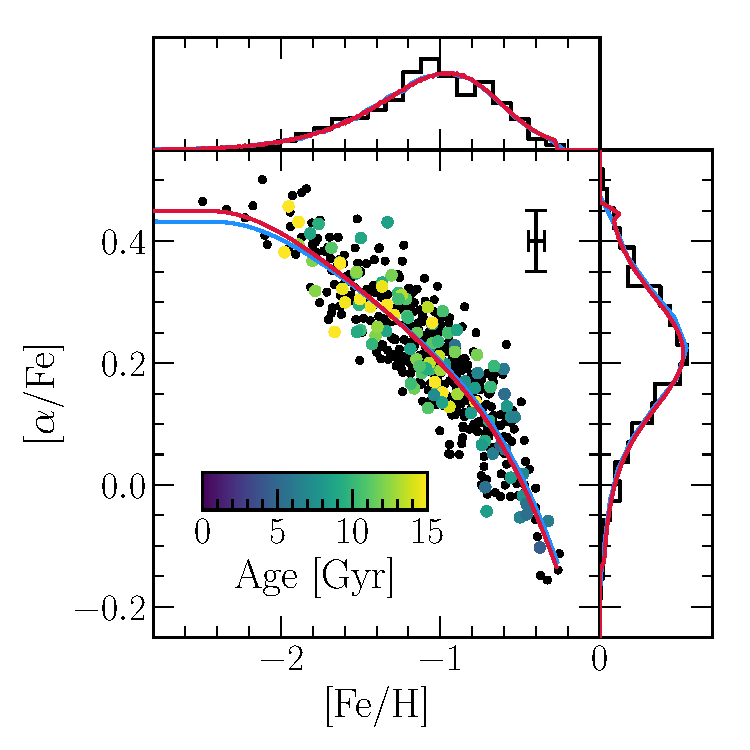
\includegraphics[scale = 0.56]{fiducial_mock_afe_feh.pdf}
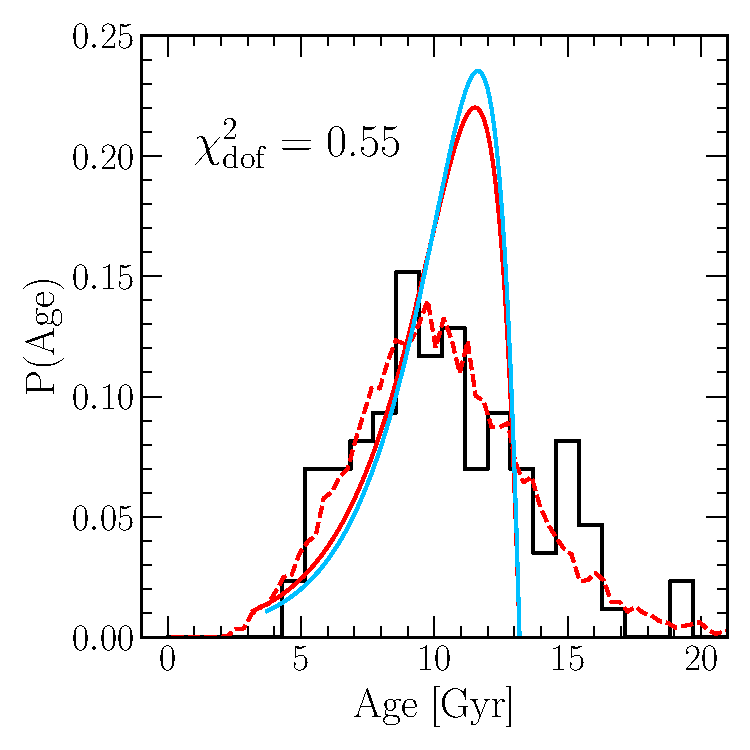
\includegraphics[scale = 0.47]{fiducial_mock_agedist.pdf}
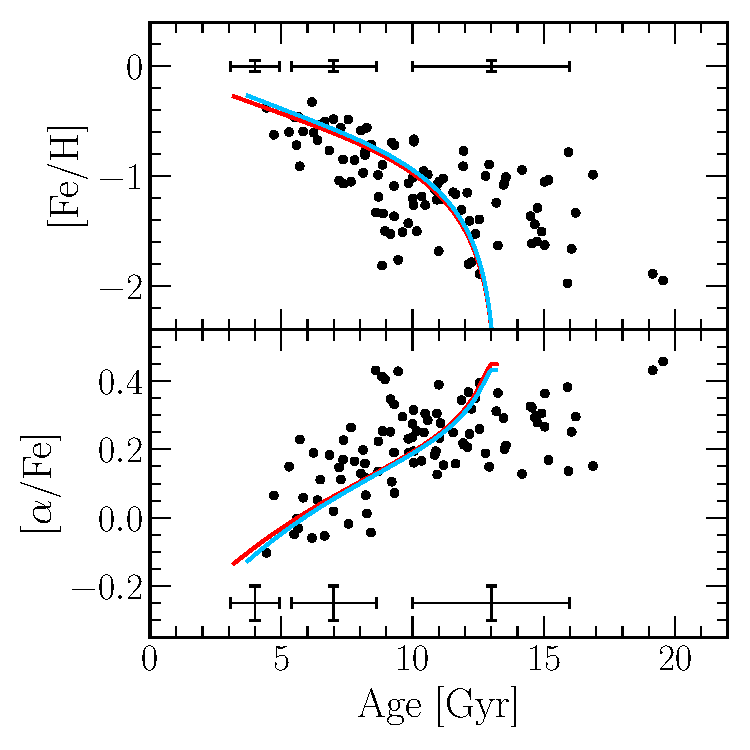
\includegraphics[scale = 0.46]{fiducial_mock_amr.pdf}
\caption{
Our fiducial mock sample.
Red lines in all panels denote the input model while blue lines denote the
recovered best-fit model.
The mock sample has~$N = 500$ stars with abundance uncertainties of
$\sigma_\feh = \sigma_\afe = 0.05$ (marked by the errorbar in the left panel).
$N = 100$ of the stars have age information as indicated by the colourbar in
the left panel with an artificial uncertainty
of~$\sigma_{\log_{10}(\text{age})} = 0.1$.
\textbf{Left}: The mock sample in chemical space, with the marginalized
distributions in~\feh~and~\afe~shown on the top and right, respectively.
\textbf{Middle}: The age distribution of the mock sample (black, binned).
The dashed red line indicates the age distribution obtained by sampling
$N = 10^4$ rather than~$N = 500$ stars from the input model and assuming the
same age uncertainty.
\textbf{Right}: The age-\feh~(top) and age-\afe~(bottom) relations for the mock
sample.
Uncertainties at various ages are marked by the error bars at the top and
bottom of each panel.
}
\label{dga:fig:fiducial_mock}
\end{figure*}
\end{landscape}
\clearpage
}

We demonstrate the accuracy of our likelihood function in~\S~\ref{dga:sec:mocks}
below by means of tests against mock data samples.
Although our likelihood function does not include a direct fit to the
stellar distributions in age and abundances, weighting the inferred likelihood
by the SFR in the model indeed incorporates this information on how many stars
should form at which ages and abundances.
Our method therefore provides~\textit{implicit} fits to the age and abundance
distributions, even though this information is not directly included in the
likelihood calculation.
\par
There are a variety of ways to construct the likelihood distribution in
parameter space.
In the present paper, we employ the MCMC method, making use of
the~\mc~\python~package~\citep{ForemanMackey2013} to construct our Markov
chains.
Despite being more computationally expensive than other methods (e.g.,
maximum a posteriori estimation), MCMC offers a more generic solution by
sampling tails and multiple modes of the likelihood distribution which could
otherwise be missed or inaccurately characterized by the assumption of
Gaussianity.
Our method should nonetheless be extensible to additional data sets described
by GCE models with different parametrizations as well as different methods of
optimizing the likelihood distribution, such as maximum a posteriori estimates.



\section{Mock Samples}
\label{dga:sec:mocks}

Using our parametrization of one-zone GCE models described
in~\S~\ref{dga:sec:onezone}, here we define a set of parameter choices from which
mock samples of stars can be drawn.
We then demonstrate the validity of our likelihood function (Eq.
\ref{dga:eq:likelihood}) in~\S~\ref{dga:sec:mocks:recovered} by applying it to a
fiducial mock sample and comparing the best-fit values to the known parameters
of the input model.
In~\S~\ref{dga:sec:mocks:variations}, we then explore variations in sample size,
measurement precision, and the availability of age information.

\subsection{A Fiducial Mock Sample}
\label{dga:sec:mocks:fiducial}

We take an exponential infall history~$\dot{M}_\text{in} \propto e^{-t /
\tau_\text{in}}$ with an e-folding timescale of~$\tau_\text{in} = 2$ Gyr and an
initial ISM mass of~$M_\text{g} = 0$.
We select an SFE timescale of~$\tau_\star = 15$ Gyr, motivated by the
observational result that dwarf galaxies have generally inefficient star
formation (e.g.,~\citealp{Hudson2015}; though not necessarily halo dwarfs that
formed in denser environments -- see discussion in~\citealt{Naidu2022}).
We additionally select a mass-loading factor of~$\eta = 10$ because the
strength of outflows should, in principle, contain information on the depth of
the gravity well of a given galaxy, with lower mass systems being more
efficient at ejecting material from the ISM.
If the SFH in this model were constant, the analytic formulae of
\citet{Weinberg2017b} suggest that the equilibrium alpha element abundance
should be~$\sim16$\% of the solar oxygen abundance, in qualitative agreement
with the empirical mass-metallicity relation for galaxies
(\citealp{Tremonti2004, Gallazzi2005};~\citealp*{Zahid2011};
\citealp{Andrews2013, Kirby2013, Zahid2014}).
\par
With these choices regarding~$\tau_\star$ and~$\eta$, our parameters are in
the regime where the normalization of the infall history, and consequently the
SFH, is inconsequential to the predicted evolution of the abundances.
The appropriate likelihood function is therefore equation~\refp{dga:eq:likelihood}
with normalized weights, whereas equation~\refp{dga:eq:lnL_minus_weights} with
un-normalized weights would be the proper form if we had selected a
parametrization in which the absolute scale of the SFH impacts the enrichment
history.
Inspection of the average SFHs predicted by the~\textsc{UniverseMachine}
semi-analytic model for galaxy formation~\citep{Behroozi2019} suggests that the
onset of star formation tends to occur a little over~$\sim$13 Gyr ago across
many orders of magnitude in stellar mass extending as low as
$\text{M}_\star \approx 10^{7.2}~\msun$.
We therefore assume that the onset of star formation occurred~$\sim$13.2 Gyr
ago, allowing~$\sim$500 Myr between the Big Bang and the first stars.
We evolve this model for 10 Gyr exactly (i.e., the youngest stars in the mock
sample have an exact age of 3.2 Gyr), stopping short of 13.2 Gyr because
surviving dwarf galaxies and stellar streams often have their star formation
quenched (e.g.,~\citealp{Monelli2010a, Monelli2010b, Sohn2013, Weisz2014a,
Weisz2014b, Weisz2015}).
These choices are not intended to resemble any one galaxy, but instead to
qualitatively resemble some disrupted dwarf galaxy whose evolutionary
parameters can be re-derived using our likelihood function as a check that it
produces accurate best-fit parameters.
\par
As discussed in~\S~\ref{dga:sec:onezone}, thoughout this paper we assume that the
IMF-averaged alpha element yield is exactly~$\yacc = 0.01$ and
$y_\alpha^\text{Ia} = 0$.
While loosely motivated by nucleosynthesis models in massive stars
\citep[e.g.,][]{Nomoto2013, Sukhbold2016, Limongi2018}, this choice is intended
to set some normalization of the effective yields which can be scaled up or
down to accommodate alternative choices.
If no scale is assumed, then extremely strong degeneracies arise in the
inferred yields, the strength of outflows~$\eta$, and the SFE timescale
$\tau_\star$ due to the yield-outflow degeneracy (see discussion in
Appendix~\ref{dga:sec:degeneracy}).
We do not distinguish between alpha elements in this validation of our
likelihood function because, from a modelling standpoint, they can all be
treated the same with a metallicity-independent yield from CCSNe and negligible
yields from all other sources (at least for the lighter alpha elements such as
O and Mg;~\citealp{Johnson2019}).
In practice, however, we take O as the canonical alpha element when integrating
these models with~\vice, adopting~$Z_{\text{O},\odot} = 0.00572$ as the
abundance of O in the sun according to~\citet{Asplund2009} and consistent with
the recent revisions of~\citet*{Asplund2021}, though similar~\afe~ratios would
arise anyway if we instead took, e.g., Mg and asserted that [O/Mg]~$\approx 0$.
\par
\citet{Weinberg2017b} adopt~$\yacc = 0.015$,~$\yfecc = 0.0012$ and
$\yfeia = 0.0017$ (see discussion in their~\S~2.2).
This massive star yield of Fe is appropriate for nucleosynthesis models in
which most~$M > 8~\msun$ stars explode as a CCSN~\citep[e.g.,][]{Woosley1995,
Chieffi2004, Chieffi2013, Nomoto2013} assuming a~\citet{Kroupa2001} IMF.
This SN Ia yield of Fe is based on the W70 explosion model of
\citet{Iwamoto1999} which produces~$\sim$0.77~\msun~of Fe per SN Ia event and
assuming that~$\scinote{2.2}{-3}~\msun^{-1}$ SNe Ia arise per solar mass of
star formation based on~\citet{Maoz2012a}.
Following these arguments, we scale these yields down by factors of~$\sim$2/3
such that $\yacc = 0.01$, adopting~$\yfecc = \scinote{8}{-4}$ and
$\yfeia = \scinote{1.1}{-3}$ in our mock samples.
We retain the assumption that~$\yacc = 0.01$ in our fits to our mock samples
but otherwise let the Fe yields~\yfecc~and~\yfeia~be free parameters to be
recovered by our likelihood function.
We use this procedure in our application to the H3 survey in~\S~\ref{dga:sec:h3}
below as well.
We then sample~$N = 500$ stars from the underlying SFH each of which have -- in
the interest of mimicking the typical precision achieved by a spectroscopic
survey of a local group dwarf galaxy --~$\sigma_\afe = \sigma_\feh = 0.05$.
100 of these stars have age measurements with an uncertainty of
$\sigma_{\log_{10}(\text{age})} = 0.1$ (i.e.,~$\sim$23\% precision).

\subsection{Recovered Parameters of the Fiducial Mock}
\label{dga:sec:mocks:recovered}

% fig 2
\begin{figure*}
\centering
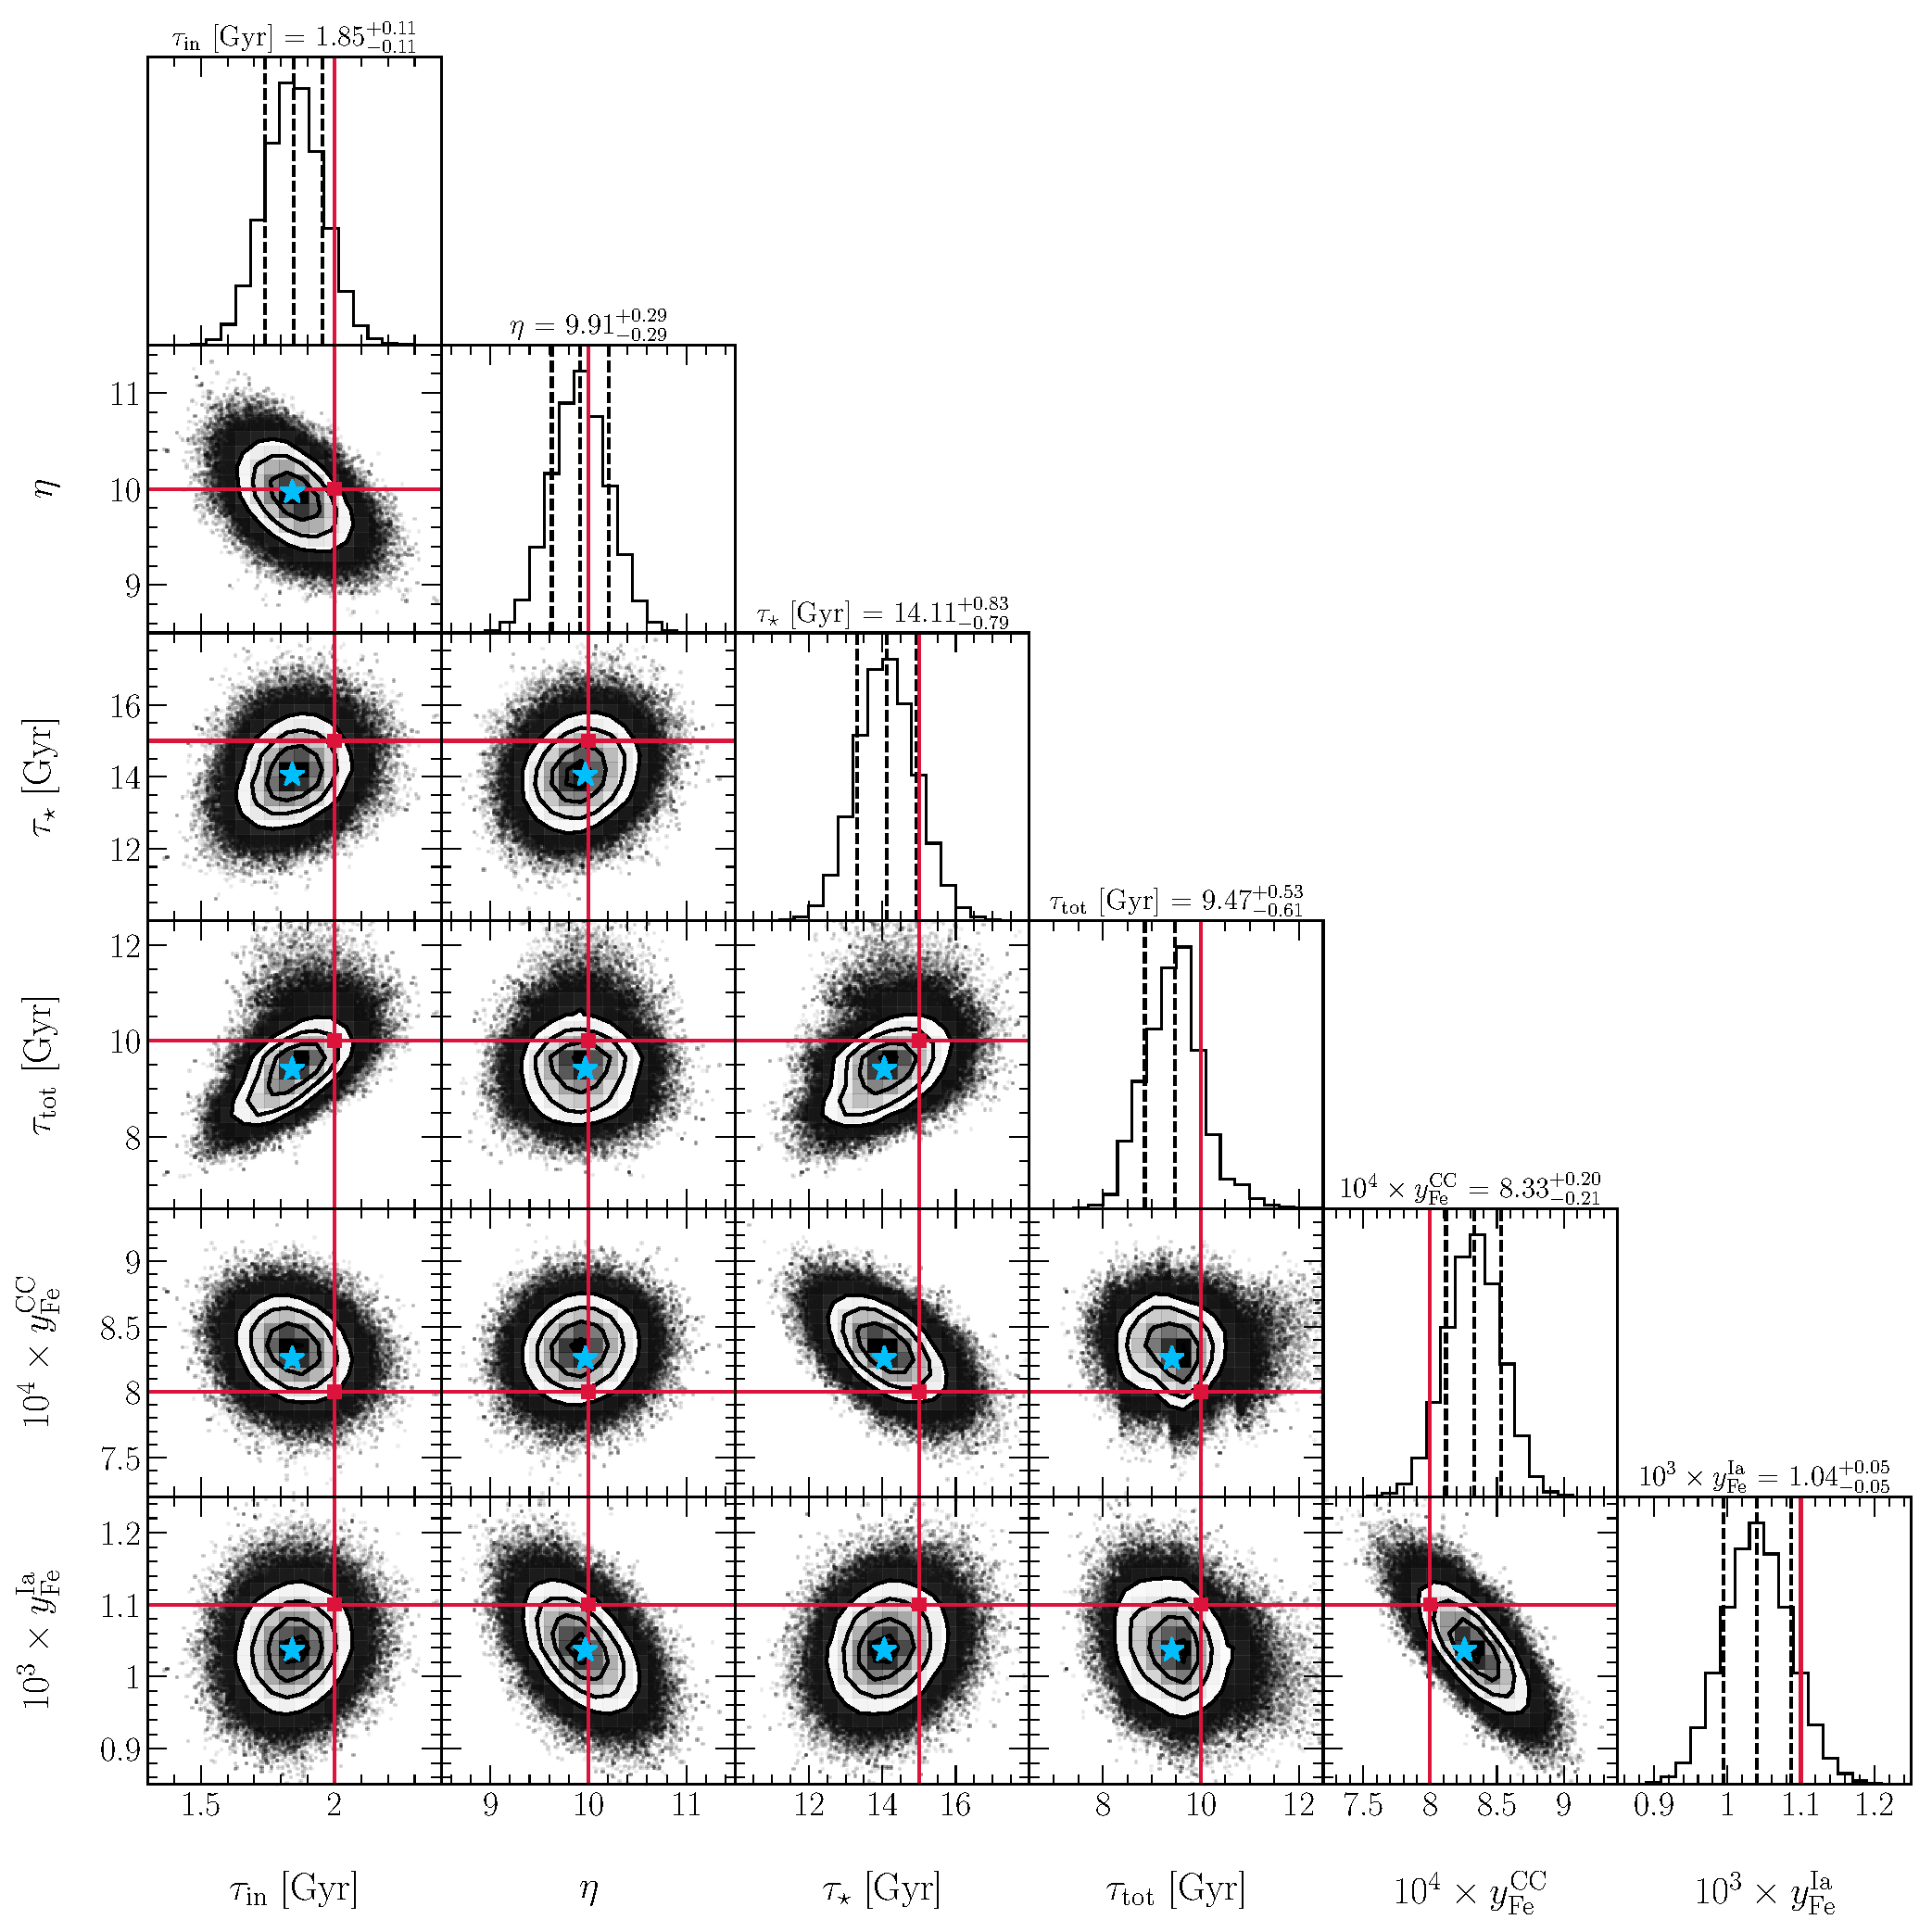
\includegraphics[scale = 0.42]{fiducial_512k.pdf}
\caption{
Posterior distributions obtained from applying our fitting method to our
fiducial mock sample (see Fig.~\ref{dga:fig:fiducial_mock} and discussion
in~\S\S~\ref{dga:sec:fitting} and~\ref{dga:sec:mocks:fiducial}).
Panels below the diagonal show 2-dimensional cross-sections of the likelihood
function while panels along the diagonal show the marginalized distributions
along with the best-fit values and confidence intervals.
Blue stars mark the element of the Markov chain with the maximum likelihood.
Red ``cross-hairs'' denote the true, known values of the parameters from the
input model (see the top row of Table~\ref{dga:tab:recovered_values}).
}
\label{dga:fig:fiducial_mock_corner}
\end{figure*}

Fig.~\ref{dga:fig:fiducial_mock} shows our fiducial mock in the observed space.
As intended by our parameter choices (see discussion
in~\S~\ref{dga:sec:mocks:fiducial}), this sample qualitatively resembles a typical
disrupted dwarf galaxy -- dominated by old stars with metal-poor
($\feh \approx -1$) and alpha-enhanced ($\afe \approx +0.2$) modes in the MDF.
We now apply the method outline in~\S~\ref{dga:sec:fitting} to recover the known
parameters of the input model.
Fig.~\ref{dga:fig:fiducial_mock_corner} shows the resulting posterior distributions,
demonstrating that our likelihood function accurately recovers each parameter.
We include the predictions of the best-fit model in Fig.~\ref{dga:fig:fiducial_mock},
finding excellent agreement with the input model.
To quantify the quality of the fit, for each datum~$\script{D}_i$ we find the
point along the track~$\script{M}_j$ with the maximum likelihood of observation
(i.e.,~$\{\script{D}_i,\script{M}_j~|~\ln L(\script{D}_i | \script{M}_j) =
\max(\ln L(\script{D}_i | \script{M}))\}$).
We then compute the chi-squared per degree of freedom diagnostic according to
\begin{equation}
\chi_\text{dof}^2 = \frac{1}{N_\text{obs} - N_\theta}
\sum_{i,j} \Delta_{ij} C_i^{-1} \Delta_{ij}^T,
\label{dga:eq:chisquared_dof}
\end{equation}
where~$N_\text{obs}$ is the number of quantities in the observed sample,
$N_\theta$ is the number of model parameteres, and the summation is taken over
the pair-wise combinations of the data and model with the maximum likelihood of
observation.
Although marginalizing over the track~\script{M}~is necessary to derive
accurate best-fit parameters (see discussion below and in~\S~\ref{dga:sec:fitting}),
it should be safe to estimate the quality of a fit by simply pairing each datum
with the most appropriate point on the track.
As noted in the middle panel of Fig.~\ref{dga:fig:fiducial_mock}, our method
achieves~$\chi_\text{dof}^2 = 0.55$, indicating that we have perhaps
over-parametrized the data.
This result is unsurprising, however, because we have fit the mock data with
the exact, known parametrization of the evolutionary history and
nucleosynthetic yields of the input model in the interest of demonstrating
proof of concept that equation~\refp{dga:eq:likelihood} provides accurate best-fit
values.
\par
Although it may appear that there are a worrying number of~$\gtrsim 1\sigma$
discrepancies in Fig.~\ref{dga:fig:fiducial_mock_corner}, we demonstrate
in~\S~\ref{dga:sec:mocks:variations} below that the differences between the known
and best-fit values here are consistent with randomly sampling from a Gaussian
distribution due to measurement uncertainty.
Although most cross sections of the posterior distribution are sufficiently
described by a multivariate Gaussian, there is some subtructure in the
likelihood distribution of~$\tau_\text{in}$, most noticeable in the
$\yfecc - \tau_\text{in}$ plane.
The MCMC algorithm naturally catches this structure, but it would be missed
under the assumption of Gaussianity as in, e.g., maximum a posteriori estimates.
There are a handful of degeneracies in the likelihood distribution of the
recovered parameters, which arise as a consequence of having an impact on the
same observable.
We discuss them individually below.
\par
% \textit{The centroid of the MDF.}
% With a fixed alpha element yield of~$\yacc = 0.01$ as we have adopted here,
% the strength of outflows~$\eta$ is set by ensuring the centroid of
% the~\ah~distribution is in agreement with the data.
% This in turn requires a total Fe yields of~$\yfecc + \yfeia$ which corresponds
% to the centroid of the~\feh~distribution.
% The total Fe yield, however, can be achieved with different breakdowns between
% CCSN and SN Ia enrichment, giving rise to the inverse relationship
% between the two Fe yields.
% \par
\textit{The height of the ``plateau'' and position of the ``knee'' in the
evolutionary track.}
The plateau in the~\afe-\feh~plane occurs in our input model
at~$\afe_\text{CC} \approx +0.45$ and arises due to the IMF-averaged massive
star yields of alpha and iron-peak elements.
The knee occurs thereafter with the onset of SN Ia enrichment, a
nucleosynthetic source of Fe but negligible amounts of alpha elements like O
and Mg~\citep{Johnson2019}.
With fixed~\yacc, variations in~\yfecc~adjust the vertical height of the
plateau.
\citet{Weinberg2017b} demonstrate that, to first order, the SFE timescale
$\tau_\star$ determines the metallicity~\feh~at which the knee occurs with
low~$\tau_\star$ models predicting a knee at high~\feh.
If a lowered plateau (i.e., higher~\yfecc) is accompanied by faster star
formation (i.e., lower~$\tau_\star$), the portion of the evolutionary track
in which~\afe~is decreasing occurs in a similar region of chemical space.
\yfecc~and~$\tau_\star$ are therefore inversely related when an overall scale
of nucleosynthetic yields is chosen.
When the overall scale is allowed to vary, we find a degeneracy of the opposite
sign (see discussion in Appendix~\ref{dga:sec:degeneracy}).
\par
\textit{The endpoint of the model track and centroid of the MDF.}
% The ratio~$\yfecc / \yfeia$ controls the drop in~\afe~between the plateau
% and the equilibrium~\afe.
These are the regions of chemical space where most of the
data are generally found, so for a given choice of~$\eta$, the~\textit{total}
Fe yield is well constrained observationally.
With only the total precisely determined,~\yfecc~and~\yfeia~are inversely
related.
On its own, adjusting~\yfeia~shifts the track vertically in the~\afe-\feh~plane
(there is horizontal movement as well, though the vertical movement is
stronger).
A downward shift in the predicted track (i.e., and increase in~$\yfeia$) can be
accompanied by a rightward shift (i.e., a decrease in~$\eta$) such that the
endpoint lies in the same location as the data.
$\yfeia$ and~$\eta$ are therefore inversely related, whereas the yield-outflow
degeneracy produces a direct relationship between these parameters
(see Appendix~\ref{dga:sec:degeneracy}).
\par
\textit{The shape of the MDF.}
The~\afe~and~\feh~distributions are affected in a handful of ways by the
parameters of this input model.
The duration of star formation has the simplest effect of cutting off the MDF
at some abundance.
Inefficient star formation (i.e., high~$\tau_\star$) increases the frequency of
low metallicity stars because it takes significantly longer for the ISM to
reach the equilibrium abundance.
Sharp infall histories (i.e., low~$\tau_\text{in}$) predict wide MDFs because
the ISM mass declines with time through losses to star formation and the lack
of replenishment by accretion.
Metals are then deposited into a ``gas-starved'' reservoir, which then reaches
higher abundances due to a deficit of hydrogen and helium.
This effect is particularly strong for Fe because of the delayed nature of SN
Ia enrichment~\citep{Weinberg2017b}.
These models achieve higher metallicities in the ISM, but their declining SFHs
produce a larger fraction of their stars early in their evolutionary history
when the abundances are lower than the late-time equilibrium abundance.
Consequently, the MDF that arises is wider for sharp infall histories but has
a peak in a similar position regardless of~$\tau_\text{in}$.
Folding these effects together, degeneracies arise in the inferred parameters
as a consequence of their effects on the MDF.
Between~$\tau_\text{in}$ and~$\tau_\text{tot}$, a sharp infall history can
broaden the MDF, but cutting off star formation earlier can allow the
distribution to remain peaked if the data suggest it.
Similarly, efficient star formation (i.e., low~$\tau_\star$) allows the ISM to
spend more time near its equilibrium abundance, enhancing the peak of the MDF,
but this change in shape can be reversed by cutting off star formation.
Between~$\tau_\text{in}$ and~$\eta$, a sharp infall history gives rise to a
high metallicity tail of the MDF, but increasing the strength of outflows
can lower the overall metallicity if this tail is too metal-rich compared to
the data.
\par
We emphasize that our fits achieve this level of precision by selecting an
overall scale for nucleosynthetic yields and outflows ($\yacc = 0.01$; see
discussion in~\S~\ref{dga:sec:onezone} and Appendix~\ref{dga:sec:degeneracy}).
Any GCE parameter that influences the centroid of the MDF or the position or
shape of the evolutionary track in abundance space is subject to the
yield-outflow degeneracy.
Given an overall scale of yields, set here by choosing~\yacc, a sample like
our fiducial mock gives quite precise constraints on all model parameters.
If we modify our choice of~\yacc, we would find similar predictions by
adjusting our Fe yields,~$\tau_\star$ and~$\eta$.
If~\yacc~is instead allowed to vary as a free parameter, then the degeneracies
are strong, but~$\tau_\text{in}$ and~$\tau_\text{tot}$ remain well constrained
due to their impact on the MDF shape.
% This includes all evolutionary parameters in our input model with the exception
% of~$\tau_\text{in}$ and~$\tau_\text{tot}$ because they impact only the shape of
% the MDF, an observational diagnostic which is constrained by a sufficiently
% large sample.
% We discuss the implications of these results applied to observed data
% in~\S~\ref{dga:sec:mocks:variations} below.
\par
In conducting these tests against mock samples, we find that the two central
features of this method are essential to ensuring the accuracy of the best-fit
parameters.
When either the weighted likelihood or the marginalization over the track
(see discussion in~\S~\ref{dga:sec:fitting}) are omitted, the fit fails to recover
the parameters of the input model with discrepancies at the many-$\sigma$ level
between the best-fit and known values.
For this reason, we caution against the reliability of GCE parameters inferred
from simplified likelihood estimates, such as matching each datum with the
nearest point on the track.


\afterpage{
\captionsetup{width=\textheight}
\begin{singlespace}
\clearpage
\renewcommand{\arraystretch}{1.5}
\begin{landscape}
% \begin{table*}
\begin{longtable}{l @{\extracolsep{\fill}} c c c c c c}
\caption{
Known (top row) and recovered best-fit values of the evolutionary parameters
of the input GCE model to out mock samples.
From left to right: the variation of our fiducial mock sample, the e-folding
timescale of the infall history~$\tau_\text{in}$, the outflow mass-loading
factor~$\eta$, the SFE timescale~$\tau_\star$, the duration of star formation
$\tau_\text{tot}$, the IMF-averaged Fe yield from CCSNe~\yfecc~and the
DTD-integrated Fe yield from SNe Ia~\yfeia.
Each variation has the same evolutionary parameters as the input model, but
has either a different sample size (top block), measurement uncertainty
in~\feh~and~\afe~abundances (top-middle block), measurement uncertainty
in~$\log_{10}(\text{age})$ (bottom-middle block), or fraction of the
sample with available age measurements (bottom block).
The values taken in the fiducial mock sample are marked in bold.
We provide illustrations of the accuracy and precision of these fits in
Figs.~\ref{dga:fig:accuracy} and~\ref{dga:fig:precision}, respectively.
}
\\
% \begin{tabularx}{\linewidth}{l @{\extracolsep{\fill}} c c c c c c}
\hline
Mock Sample & $\tau_\text{in}$ [Gyr] & $\eta$ & $\tau_\star$ [Gyr] &
$\tau_\text{tot}$ [Gyr] & \yfecc~[$\times 10^{-4}$] & \yfeia~[$\times 10^{-3}$]
\\
\hline
\null &
2 &
10  &
15 &
10 &
8.00 &
1.10
\\
\hline
$N = 20$ &
$2.55^{+0.75}_{-0.45}$ &
$8.39^{+1.11}_{-1.30}$  &
$14.35^{+5.56}_{-3.32}$ &
$10.60^{+1.65}_{-1.09}$ &
${7.90^{+1.20}_{-1.90}}$ &
${1.36^{+0.33}_{-0.23}}$
\\
$N = 50$ &
$2.13^{+0.42}_{-0.36}$ &
$10.39^{+0.80}_{-0.76}$  &
$13.75^{+2.79}_{-2.38}$ &
$11.25^{+1.37}_{-1.76}$ &
${8.30 \pm 0.60}$ &
${0.95 \pm 0.14}$
\\
$N = 100$ &
$2.06^{+0.27}_{-0.26}$ &
$9.88^{+0.64}_{-0.62}$  &
$15.06^{+2.00}_{-1.79}$ &
$11.52^{+1.06}_{-1.30}$ &
$8.10 \pm 0.40$ &
$1.08 \pm 0.09$
\\
$N = 200$ &
$2.10^{+0.18}_{-0.17}$ &
$10.11^{+0.45}_{-0.43}$  &
$14.61^{+1.34}_{-1.18}$ &
$10.60^{+1.07}_{-0.86}$ &
$7.70 \pm 0.30$ &
$1.14 \pm 0.07$
\\
$\bm{N = 500}$ &
$\bm{1.85 \pm 0.11}$ &
$\bm{9.91 \pm 0.29}$  &
$\bm{14.11^{+0.83}_{-0.79}}$ &
$\bm{9.47^{+0.53}_{-0.61}}$ &
$\bm{8.30^{+0.20}_{-0.21}}$ &
$\bm{1.04 \pm 0.05}$
\\
$N = 1000$ &
$2.05^{+0.09}_{-0.08}$ &
$9.72 \pm 0.20$  &
$14.62^{+0.57}_{-0.56}$ &
$9.83^{+0.38}_{-0.39}$ &
$8.10 \pm 0.10$ &
$1.14 \pm 0.03$
\\
$N = 2000$ &
$2.00 \pm 0.05$ &
$10.26 \pm 0.15$  &
$15.82^{+0.44}_{-0.42}$ &
$10.30^{+0.25}_{-0.32}$ &
$8.00 \pm 0.10$ &
$1.09 \pm 0.02$
\\
\hline
$\sigma_\text{[X/Y]} = 0.01$ &
$1.89 \pm 0.10$ &
$10.25 \pm 0.28$  &
$15.06^{+0.52}_{-0.47}$ &
$9.70^{+0.51}_{-0.59}$ &
$8.00 \pm 0.10$ &
$1.09 \pm 0.02$
\\
$\sigma_\text{[X/Y]} = 0.02$ &
$1.92^{+0.10}_{-0.09}$ &
$10.10 \pm 0.25$  &
$14.71^{+0.56}_{-0.55}$ &
$9.79^{+0.45}_{-0.40}$ &
$8.10 \pm 0.10$ &
$1.08^{+0.02}_{-0.03}$
\\
$\bm{\sigma_\textbf{[X/Y]} = 0.05}$ &
$\bm{1.85 \pm 0.11}$ &
$\bm{9.91 \pm 0.29}$  &
$\bm{14.11^{+0.83}_{-0.79}}$ &
$\bm{9.47^{+0.53}_{-0.61}}$ &
$\bm{8.30^{+0.20}_{-0.21}}$ &
$\bm{1.04 \pm 0.05}$
\\
$\sigma_\text{[X/Y]} = 0.1$ &
$2.00^{+0.13}_{-0.12}$ &
$9.88^{+0.31}_{-0.33}$  &
$13.39 \pm 1.02$ &
$11.10^{+1.00}_{-0.84}$ &
$8.50^{+0.40}_{-0.30}$ &
$1.01 \pm 0.07$
\\
$\sigma_\text{[X/Y]} = 0.2$ &
$2.22 \pm 0.21$ &
$9.83^{+0.58}_{-0.67}$  &
$18.21^{+2.19}_{-2.02}$ &
$10.32^{+1.05}_{-0.67}$ &
$8.70 \pm 0.70$ &
$1.05 \pm 0.14$
\\
$\sigma_\text{[X/Y]} = 0.5$ &
$2.73^{+0.82}_{-0.60}$ &
$10.05^{+1.22}_{-1.26}$  &
$12.52^{+3.75}_{-3.35}$ &
$9.00^{+1.26}_{-0.95}$ &
$7.50^{+1.80}_{-1.60}$ &
$1.12 \pm 0.31$
\\
\hline
$\sigma_{\log_{10}(\text{age})} = 0.02$ &
$2.08^{+0.09}_{-0.08}$ &
$9.84^{+0.24}_{-0.26}$  &
$14.69^{+0.50}_{-0.46}$ &
$10.41^{+0.47}_{-0.41}$ &
$8.10 \pm 0.20$ &
$1.11^{+0.05}_{-0.04}$
\\
$\sigma_{\log_{10}(\text{age})} = 0.05$ &
$1.96 \pm 0.11$ &
$9.88^{+0.32}_{-0.30}$  &
$15.70^{+0.71}_{-0.68}$ &
$9.95^{+0.63}_{-0.53}$ &
$8.00 \pm 0.20$ &
$1.11^{+0.05}_{-0.04}$
\\
$\bm{\sigma_{\log_{10}(\textbf{age})} = 0.1}$ &
$\bm{1.85 \pm 0.11}$ &
$\bm{9.91 \pm 0.29}$  &
$\bm{14.11^{+0.83}_{-0.79}}$ &
$\bm{9.47^{+0.53}_{-0.61}}$ &
$\bm{8.30^{+0.20}_{-0.21}}$ &
$\bm{1.04 \pm 0.05}$
\\
$\sigma_{\log_{10}(\text{age})} = 0.2$ &
$2.20^{+0.18}_{-0.17}$ &
$9.83^{+0.28}_{-0.27}$  &
$15.19 \pm 1.11$ &
$10.76^{+0.85}_{-0.93}$ &
$8.00 \pm 0.20$ &
$1.11^{+0.05}_{-0.04}$
\\
$\sigma_{\log_{10}(\text{age})} = 0.5$ &
$2.25^{+0.20}_{-0.25}$ &
$9.86^{+0.28}_{-0.30}$  &
$16.24^{+1.44}_{-1.62}$ &
$11.38^{+1.00}_{-1.34}$ &
$8.00 \pm 0.20$ &
$1.10 \pm 0.05$
\\
$\sigma_{\log_{10}(\text{age})} = 1$ &
$1.69^{+0.35}_{-0.32}$ &
$9.53 \pm 0.29$  &
$12.38^{+2.27}_{-2.08}$ &
$8.66^{+1.86}_{-1.74}$ &
$8.30 \pm 0.30$ &
$1.15 \pm 0.06$
\\
\hline
$f_\text{age} = 0$ &
$1.65^{+0.55}_{-0.37}$ &
$9.39^{+0.30}_{-0.29}$  &
$11.80^{+3.36}_{-2.44}$ &
$7.35^{+2.62}_{-1.74}$ &
$8.30 \pm 0.40$ &
$1.19^{+0.08}_{-0.07}$
\\
$f_\text{age} = 0.1$ &
$1.75^{+0.16}_{-0.17}$ &
$10.06^{+0.29}_{-0.28}$  &
$13.65^{+1.22}_{-1.12}$ &
$8.84 \pm 0.87$ &
$8.40 \pm 0.20$ &
$1.06 \pm 0.05$
\\
$\bm{f_\textbf{age} = 0.2}$ &
$\bm{1.85 \pm 0.11}$ &
$\bm{9.91 \pm 0.29}$  &
$\bm{14.11^{+0.83}_{-0.79}}$ &
$\bm{9.47^{+0.53}_{-0.61}}$ &
$\bm{8.30^{+0.20}_{-0.21}}$ &
$\bm{1.04 \pm 0.05}$
\\
$f_\text{age} = 0.3$ &
$1.94^{+0.11}_{-0.10}$ &
$9.80^{+0.27}_{-0.28}$  &
$14.26^{+0.74}_{-0.67}$ &
$9.89^{+0.54}_{-0.48}$ &
$8.00 \pm 0.20$ &
$1.10 \pm 0.04$
\\
$f_\text{age} = 0.4$ &
$1.91^{+0.09}_{-0.10}$ &
$10.07^{+0.32}_{-0.30}$  &
$16.79^{+0.81}_{-0.83}$ &
$10.34^{+0.61}_{-0.50}$ &
$7.80 \pm 0.20$ &
$1.12 \pm 0.05$
\\
$f_\text{age} = 0.5$ &
$2.00 \pm 0.10$ &
$10.16^{+0.30}_{-0.29}$  &
$15.46^{+0.70}_{-0.69}$ &
$9.83^{+0.48}_{-0.40}$ &
$7.80 \pm 0.20$ &
$1.12^{+0.05}_{-0.04}$
\\
$f_\text{age} = 0.6$ &
$2.18 \pm 0.09$ &
$9.65^{+0.27}_{-0.25}$  &
$14.25^{+0.67}_{-0.64}$ &
$10.49^{+0.44}_{-0.37}$ &
$7.80 \pm 0.20$ &
$1.15 \pm 0.04$
\\
$f_\text{age} = 0.7$ &
$1.99 \pm 0.08$ &
$9.81^{+0.28}_{-0.27}$  &
$14.92^{+0.68}_{-0.62}$ &
$10.25^{+0.46}_{-0.37}$ &
$8.10 \pm 0.20$ &
$1.08 \pm 0.04$
\\
$f_\text{age} = 0.8$ &
$2.06 \pm 0.09$ &
$9.53^{+0.29}_{-0.26}$  &
$15.18^{+0.63}_{-0.59}$ &
$9.76^{+0.36}_{-0.33}$ &
$7.90 \pm 0.20$ &
$1.15 \pm 0.05$
\\
$f_\text{age} = 0.9$ &
$1.93 \pm 0.08$ &
$10.41 \pm 0.31$  &
$16.23^{+0.73}_{-0.70}$ &
$10.03^{+0.39}_{-0.33}$ &
$7.70 \pm 0.20$ &
$1.14 \pm 0.04$
\\
$f_\text{age} = 1$ &
$2.13 \pm 0.09$ &
$9.44^{+0.28}_{-0.27}$  &
$15.67^{+0.64}_{-0.60}$ &
$10.21^{+0.35}_{-0.31}$ &
$8.00 \pm 0.20$ &
$1.15 \pm 0.05$
\\
\hline
% \end{tabularx}
\label{dga:tab:recovered_values}
% \end{table*}
\end{longtable}
\end{landscape}
\clearpage
\end{singlespace}
} % afterpage



% fig 3
\begin{figure*}
\centering
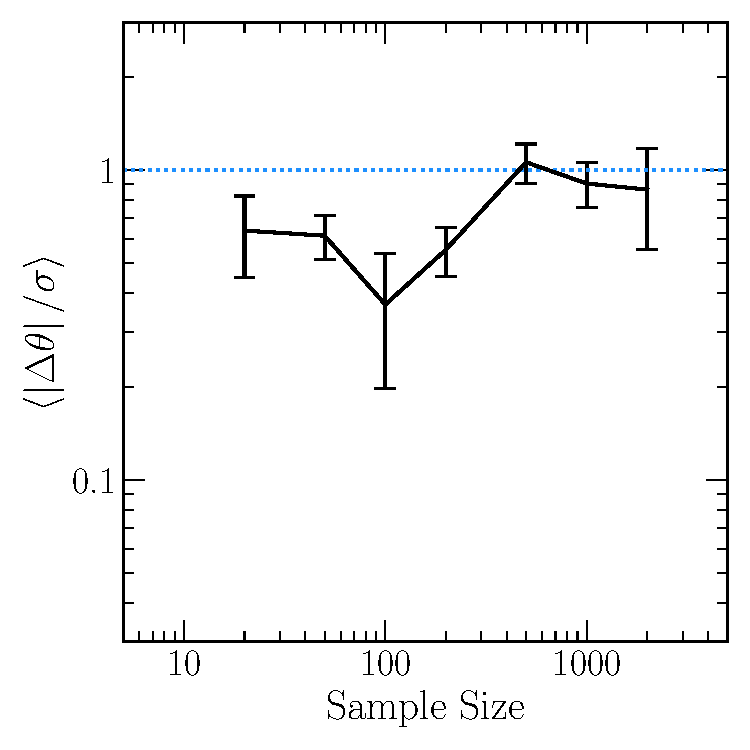
\includegraphics[scale = 0.42]{dp_sigma_samplesize.pdf}
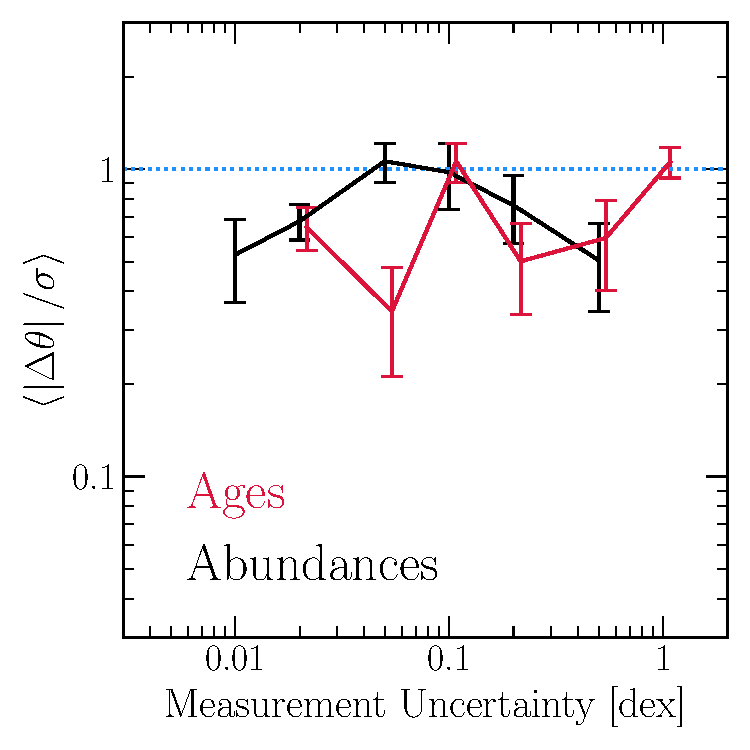
\includegraphics[scale = 0.42]{dp_sigma_precision.pdf}
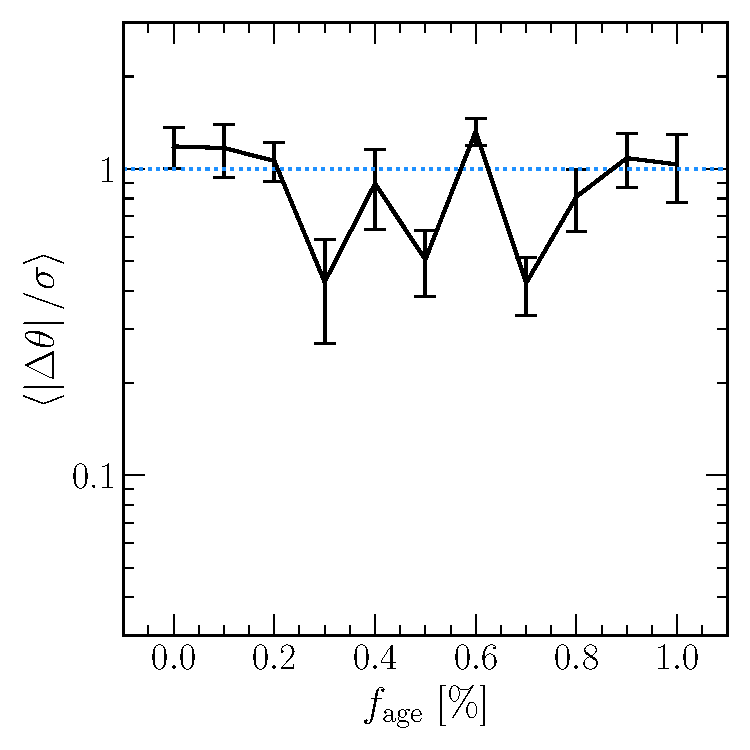
\includegraphics[scale = 0.42]{dp_sigma_agefrac.pdf}
\caption{
Differences between input model parameters and recovered best-fit values.
Each point is the mean deviation~$\left|\Delta\theta\right|$ for each of the
six free parameters in Table~\ref{dga:tab:recovered_values} (i.e.,
$\{\theta\} = \{\tau_\text{in}, \eta, \tau_\star, \tau_\text{tot}, \yfecc,
\yfeia\}$) in units of the best-fit uncertainty~$\sigma$.
Our mock samples vary in terms of their sample size (left), measurement
precision in~\feh~and~\afe~abundances (middle, black), measurement precision in
$\log_{10}(\text{age})$ (middle, red), and the fraction of the sample with
available age measurements (right).
Error bars denote the error in the mean deviation of the six free parameters.
Blue dotted lines mark~$\langle \Delta \theta / \sigma \rangle = 1$, the
expected mean offset due to randomly sampling from a Gaussian distribution.
}
\label{dga:fig:accuracy}
\end{figure*}

\subsection{Variations in Sample Size, Measurement Precision and the
Availability of Age Information}
\label{dga:sec:mocks:variations}

We now explore variations of our fiducial mock sample.
We retain the same evolutionary parameters of the input model (see discussion
in~\S~\ref{dga:sec:mocks:fiducial}), but each variant differs in one of the
following:
\begin{itemize}

	\item Sample size.

	\item Measurement precision in~\feh~and~\afe.

	\item Measurement precision in~$\log_{10}(\text{age})$.

	\item The fraction of the sample that has age measurements.

\end{itemize}
The left-hand column of Table~\ref{dga:tab:recovered_values} provides a summary of
the values we take as exploratory cases with the fiducial mock marked in bold.
In the remaining columns, we provide the associated values derived for each
GCE parameter~$\theta$ along with their~$1\sigma$ confidence intervals.
The sample sizes we consider are intended to reflect the range that is
typically achieved in disrupted dwarf galaxies where the proximity might
allow individual age estimates for main sequence turnoff stars.
Because of their distance and low stellar mass, dwarf galaxies are considerably
less conducive to the large sample sizes achieved by Milky Way surveys like
APOGEE~\citep{Majewski2017} and GALAH~\citep{DeSilva2015, Martell2017}.
Our choices in measurement precision are intended to reflect typical values
achieved by modern spectroscopic surveys.
Although deriving elemental abundances through spectroscopy is a nontrivial
problem known to be affected by systematics~\citep[e.g.,][]{Anguiano2018},
stellar age measurements
are generally the more difficult of the two~\citep{Soderblom2010, Chaplin2013}.
The age measurements may therefore be available for only a small portion of the
sample and are often less precise than the abundances ($f_\text{age} = 20$\%
and~$\sigma_\feh = \sigma_\afe = 0.05$ versus
$\sigma_{\log_{10}(\text{age})} = 0.1$ in our fiducial mock).
In practice, however, uncertainties vary with stellar mass; for example, hot
main sequence turnoff stars have precise ages but poorly constrained
abundances due to the lack of lines in their spectra.
\par
Fig.~\ref{dga:fig:accuracy} demonstrates the accuracy of our fitting method with
respect to variations in these details surrounding the data.
We compute the deviation between each re-derived parameter~$\theta$
(i.e.,~$\tau_\text{in}$,~$\eta$,~$\tau_\star$, etc.) and its known value from
the input model, then divide by the fit uncertainty~$\sigma_\theta$ and plot
the mean on the y-axis.
Under all variants that we explore, our likelihood function accurately recovers
the input parameters to~$\sim1\sigma$ or slightly better.
This deviation is exactly as expected when the uncertainties are described by a
Gaussian random process, wherein the most likely deviation from the true value
is exactly~$1\sigma$.
This expectation holds even with infinite data, though in that limit
the~$1\sigma$ uncertainty interval becomes arbitrarily small.
This demonstrates that equation~\refp{dga:eq:likelihood} provides accurate best-fit
parameters even when the sample size is as low as~$N \approx 20$, when the
measurement uncertainties are as imprecise as~$\sigma_\text{[X/Y]} \approx 0.5$
and~$\sigma_{\log_{10}(\text{age})} \approx 1$, or even when there is no age
information available at all.
The precision of the fit will indeed suffer in such cases (see Fig.
\ref{dga:fig:precision} and associated discussion below), but the inferred
parameters will remain accurate nonetheless.

% fig 4
\begin{figure*}
\centering
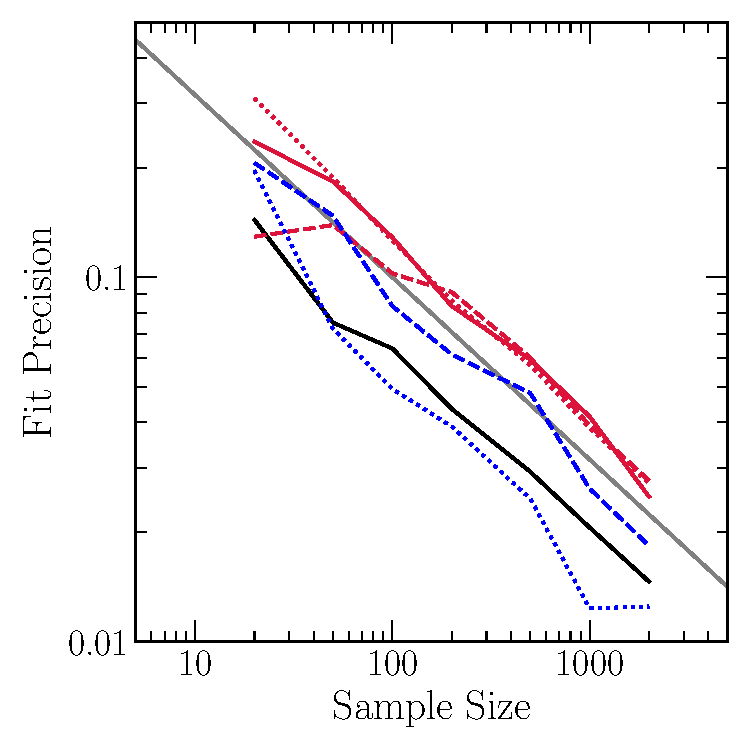
\includegraphics[scale = 0.55]{precision_samplesize.pdf}
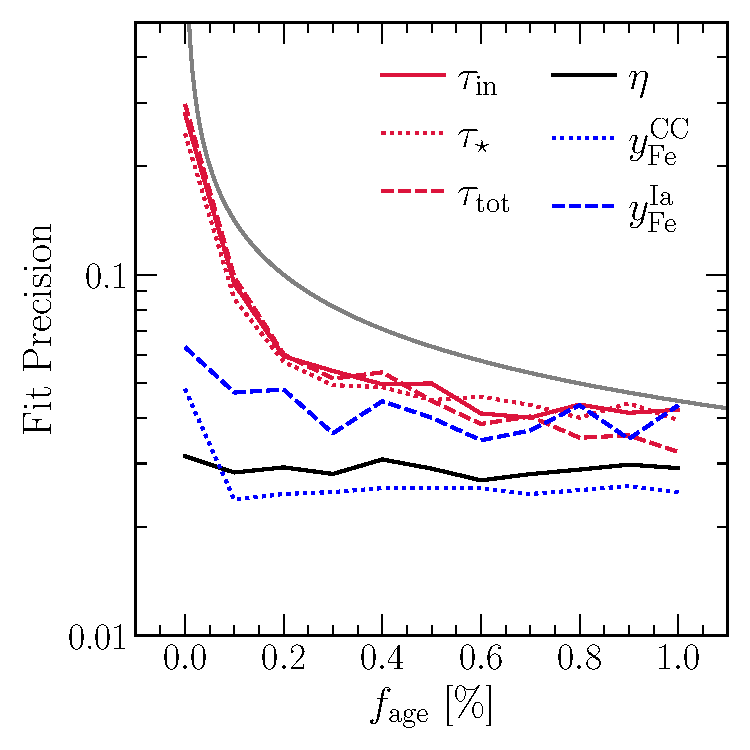
\includegraphics[scale = 0.55]{precision_agefrac.pdf}
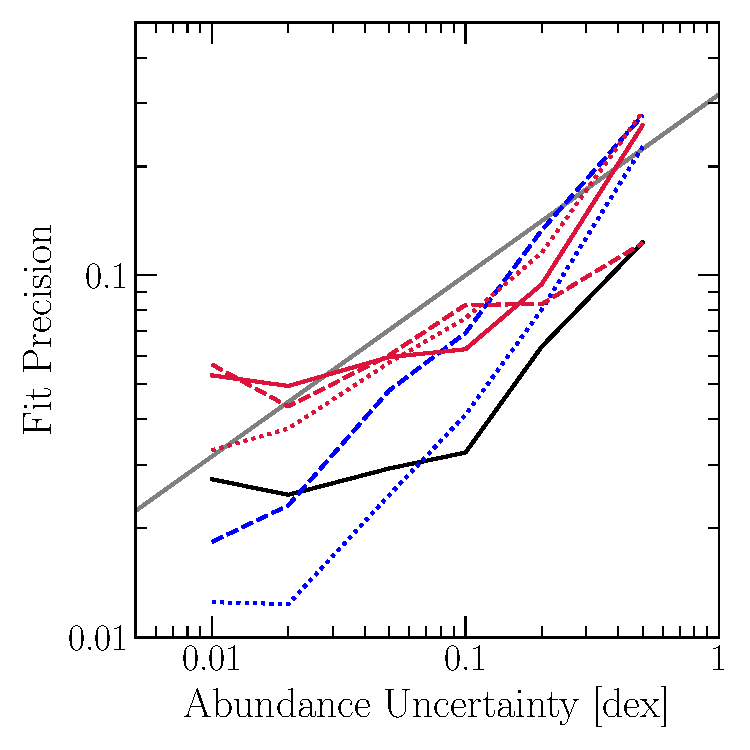
\includegraphics[scale = 0.55]{precision_abundanceuncertainty.pdf}
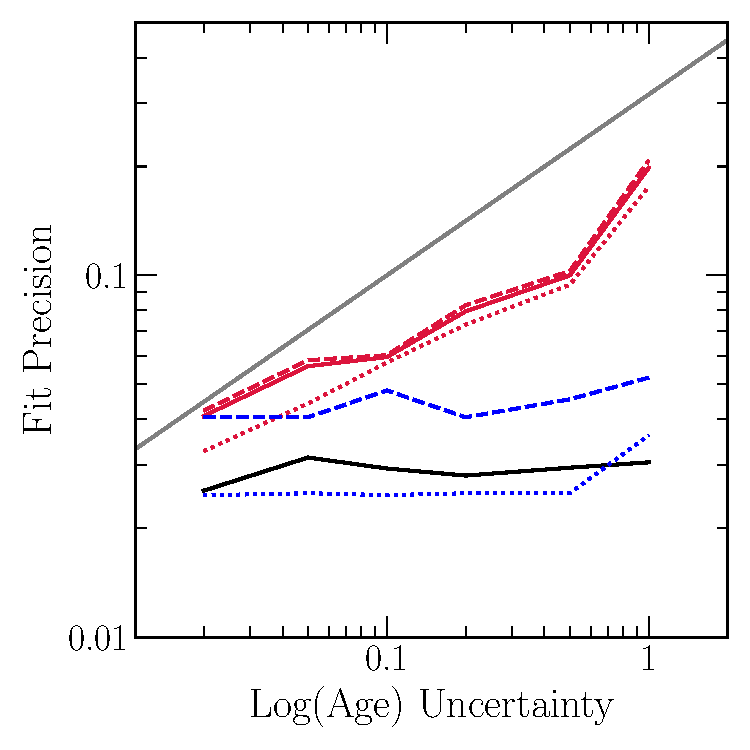
\includegraphics[scale = 0.55]{precision_ageuncertainty.pdf}
\caption{
Precision of our fitting method.
For a fit uncertainty~$\sigma$ and deviation from the known value
$\Delta\theta$, we compute precision according to
$\left|\Delta\theta\right| / \sigma$ for each of the six free parameters
in Table~\ref{dga:tab:recovered_values} and plot them as a function
of sample size (top left), the fraction of the sample with age information (top
right), abundance uncertainties (bottom left), and age uncertainties (bottom
right).
Grey lines in each panel denote~$x^{\pm0.5}$ scaling where~$x$ is the quantity
on the~$y$-axis.
We plot timescales in red, Fe yields in blue, and the mass-loading
factor~$\eta$ in black in all panels according to the legend.
}
\label{dga:fig:precision}
\end{figure*}

We have explored alternate parametrizations of our mock sample's evolutionary
history and indeed found that our method accurately recovers the parameters
in all cases.
For example, one is a case in which we build in a significant starburst,
finding that we accurately recover both the timing and the strength of the
burst.
We have also explored an infall rate that varies sinusoidally about some mean
value, mimicking natural fluctuations in the accretion history or a series of
minor starbursts.
Although idealized and potentially unrealistic, our likelihood function
accurately recovers the amplitude, phase and frequency in this case as well.
Of course, the parametrization itself must allow for such possibilities, but
we stick to smooth SFHs for the remainder of these tests.
\par
Fig.~\ref{dga:fig:precision} demonstrates how the uncertainty of each best-fit
parameter is affected by these details of the sample.
With differences in the normalization, the precision of each inferred parameter
scales with sample size approximately as~$N^{-0.5}$.
In general, the mass-loading factor~$\eta$ and the Fe yields are constrained
more precisely than the timescales.
The primary exception to this rule is when the abundance uncertainties are
large compared to the age uncertainties, in which case the Fe yields are
constrained to a similar precision as~$\tau_\text{in}$ and~$\tau_\star$
but~$\tau_\text{tot}$ is determined more precisely.
The Fe yields are, unsurprisingly, the most sensitive parameters to the
abundance uncertainties, while~$\eta$ can be determined with~$\sim$10\% precision
even with highly imprecise measurements ($\sigma_\text{[X/Y])} \approx 0.5$).
Even with imprecise abundances, the centroid of the MDF can still be robustly
determined with a sufficiently large sample, which allows a precise inference
of the strength of winds due to its impact on the equilibrium metallicity (for
an assumed scale of nucleosynthetic yields such as~$\yacc = 0.01$ in this
paper).
\par
Only the inferred timescales are impacted by the availability of age
information and the uncertainties thereof.
Even with order of magnitude uncertainties in stellar ages, however, the
evolutionary timescales of our mock samples are recovered to~$\sim$20\%
precision.
Interestingly the introduction of age information to the sample impacts the
fit uncertainty only for~$f_\text{age} \lesssim 30$\%.
Above this value, there is only marginal gain in the precision of best-fit
timescales.
These results suggest that authors seeking to determine best-fit evolutionary
parameters for one-zone models applied to any sample should focus their efforts
on sample size and precise abundance measurements with age information being
a secondary consideration.
Thankfully, abundances are generally easier than ages to measure on a
star-by-star basis~\citep{Soderblom2010, Chaplin2013}.



\section{Application to Observations}
\label{dga:sec:h3}

We now apply our likelihood function (Eq.~\ref{dga:eq:likelihood}) to two
disrupted dwarf galaxies in the Milky Way stellar halo.
The first is a relatively well-studied system: GSE~\citep{Belokurov2018,
Helmi2018, Haywood2018, Myeong2018, Mackereth2019}, believed to be responsible
for a major merger event early in the Milky Way's history~\citep{Gallart2019,
Bonaca2020, Chaplin2020, Montalban2021, Xiang2022} which
contributed~$\sim$$10^9~\msun$ of total stellar mass to the Galaxy
\citep{Deason2019, Fattahi2019, Mackereth2019, Vincenzo2019b, Kruijssen2020,
Han2022}, including eight globular clusters in the stellar
halo~\citep{Myeong2018, Massari2019, Kruijssen2019, Forbes2020}.
GSE is a good test case for this method both because it is the dominant
structure in the Milky Way's inner halo~\citep{Helmi2018} and because we can
compare to independent constraints thanks to the amount of attention it has
received in the literature.

\subfile{results.tablebody.tex}

The second is a less well-studied system: Wukong/LMS-1, a structure chemically
distinct from GSE which sits between it and the Helmi stream~\citep{Helmi1999}
in energy-angular momentum space~\citep{Naidu2020, Yuan2020} that
formed from an M$_\star \approx \scinote{1.3}{7}~\msun$ disrupted
galaxy~\citep{Naidu2022}.
Wukong/LMS-1 is an interesting system to investigate with our method
because it displays a ``classic'' enrichment history with an obvious ``knee''
in the evolutionary track near~$\feh \approx -2.8$ (see Fig.~\ref{dga:fig:wukong}
below).
It has been associated~\citep{Malhan2022} with the most metal-poor streams in
the halo~\citep[e.g.,][]{Roederer2019, Wan2020, Martin2022} and a high fraction
of carbon-enhanced metal-poor stars given its low stellar mass
\citep{Shank2022, Zepeda2023}, marking it as a disrupted dwarf with a
potentially remarkable chemical history.
We make use of data from the H3 survey (see discussion
in~\S~\ref{dga:sec:h3:survey} below) and discuss our GCE model fits to GSE and
Wukong/LMS-1 in~\S\S~\ref{dga:sec:h3:gse} and~\ref{dga:sec:h3:wukong}, comparing our
results for the two galaxies in~\S~\ref{dga:sec:h3:comparison}.

\subsection{The H3 Survey}
\label{dga:sec:h3:survey}

The H3 survey~\citep{Conroy2019} is collecting medium-resolution spectra
of~$\sim$300,000 stars in high-latitude fields ($\left|b\right| > 20^\circ$).
Spectra are collected from the Hectochelle instrument on the MMT
\citep{Szentgyorgyi2011}, which delivers~$R \approx$~32,000 spectra over the
wavelength range of~$5150 - 5300$~\AA.
Spectral lines in this wavelength range are dominated by iron-peak elements and
the MgI triplet (see Fig. 6 of~\citealt{Conroy2019}).
Throughout this section, the alpha element abundances we refer to are therefore
Mg abundances specifically, whereas in previous sections an alpha element
refers to any species where the only statistically significant enrichment
source is a metallicity-dependent yield from massive stars.
\par
The survey selection function is deliberately simple: the primary sample
consists of stars with~$r$ band magnitudes of~$15 < r < 18$
and~\gaia~\citep{GaiaCollaboration2016} parallaxes~$<$ 0.3 mas (this threshold
has evolved over the course of the survey as the~\gaia~astrometry has become
more precise).
Stellar parameters are estimated by the~\textsc{MINESweeper} program
\citep{Cargile2020}, which fits grids of isochrones, synthetic spectra and
photometry to the Hectochelle spectrum and broadband photometry from~\gaia,
Pan-STARRS~\citep{Chambers2016}, SDSS~\citep{York2000}, 2MASS
\citep{Skrutskie2006} and WISE~\citep{Wright2010} with the~\gaia~parallax
used as a prior.
The fitted parameters include radial velocity, spectrophotometric distance,
reddening,~\feh,~\afe~and age.
The default analysis includes a complicated prior on age and distance
(see~\citealt{Cargile2020} for details).
We have also re-fit high signal-to-noise data with a flat age prior for cases
where ages play an important role.
In this paper we use the catalog which uses this flat age prior.

\subsection{\gaia-Sausage Enceladus}
\label{dga:sec:h3:gse}

% fig 5
\begin{figure*}
\centering
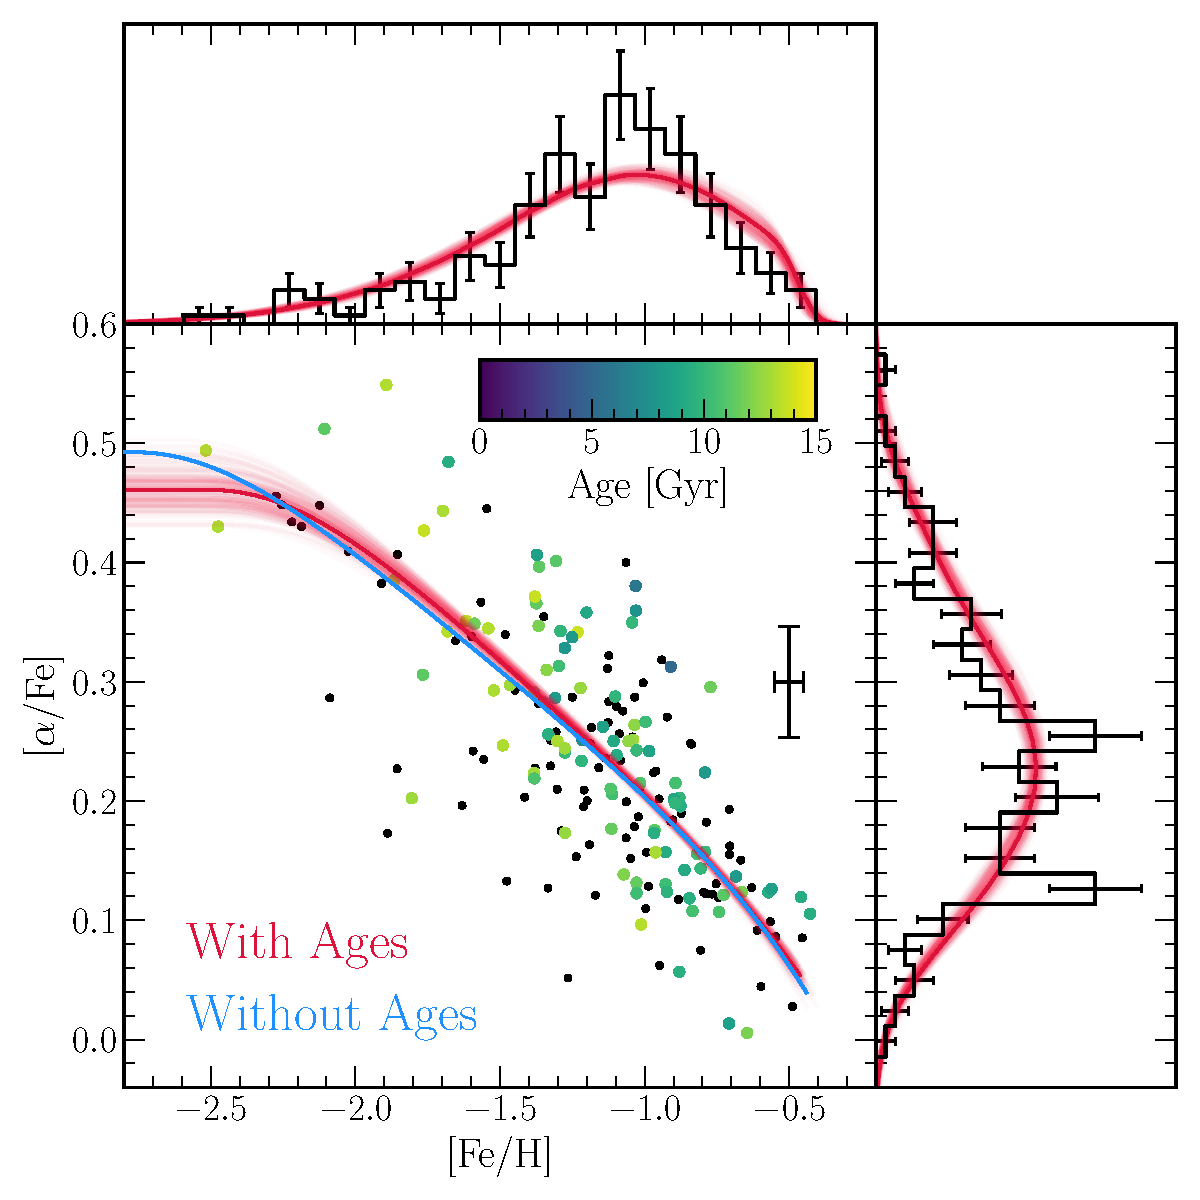
\includegraphics[scale = 0.65]{gsefit_afe_feh.pdf}
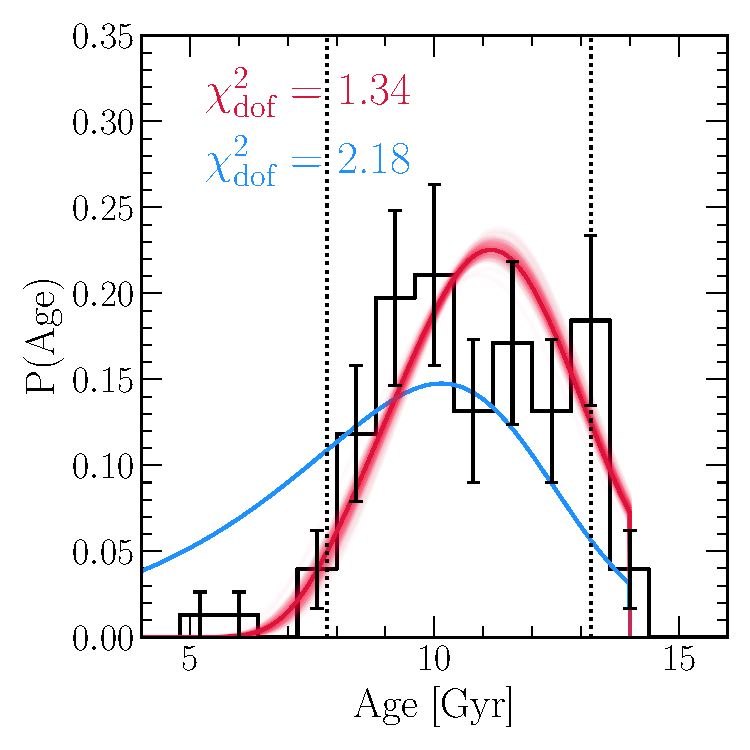
\includegraphics[scale = 0.54]{gsefit_agedist.pdf}
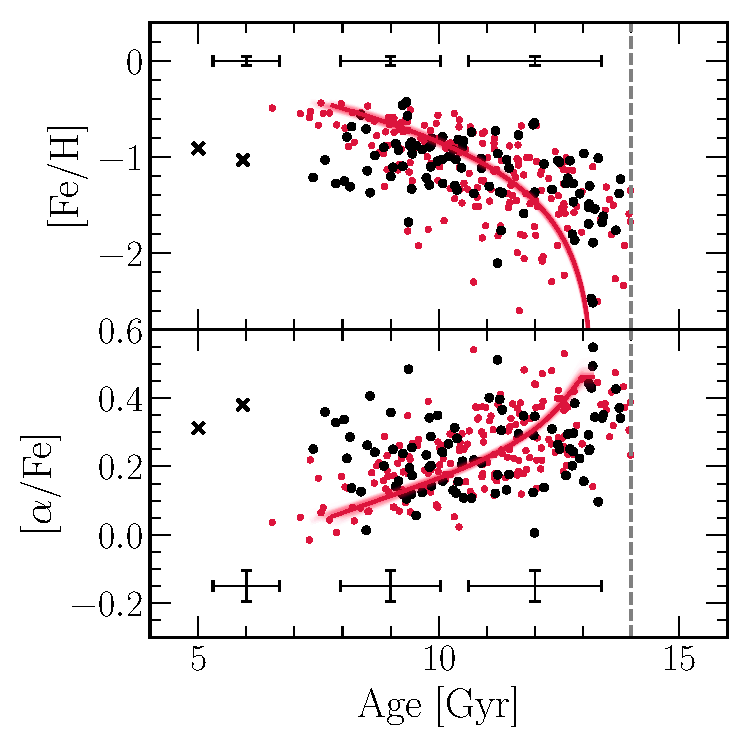
\includegraphics[scale = 0.53]{gsefit_amr.pdf}
\caption{
Our GSE sample.
Red lines in all panels denote the best-fit one-zone model, while the
blue lines in the top and bottom left panels denote the best-fit model obtained
when excluding age measurements from the fit.
Distributions in~\feh,~\afe~and age are convolved with the median uncertainty
of the sample (see discussion in~\S~\ref{dga:sec:h3:gse}).
We additionally subsample 200 sets of parameter choices from our Markov chain
and plot their predictions as highly transparent lines to offer a sense of the
fit uncertainty.
Error bars in each distribution indicate a~$\sqrt{N}$ uncertainty associated
with random sampling.
\textbf{Top}: Our sample in chemical space and the associated marginalized
distributions.
Stars with age measurements are colour coded accordingly and are otherwise
plotted in black.
The median~\feh~and~\afe~uncertainty in the sample is shown by the error bar
to the right of the data.
\textbf{Bottom left}: The age distribution of our GSE sample (black,
binned).
\textbf{Bottom right}: Age-\feh~(top) and age-\afe~(bottom) relations
The median~\feh,~\afe~and age uncertainties are shown by the error bars at the
top and bottom of each panel.
We plot the two stars that we exclude from our fit as black X's (likely
blue stragglers; see discussion in~\S~\ref{dga:sec:h3:gse}).
Red points denote~$N = 95$ stars (the same size as the stars with ages in our
GSE sample) drawn from out best-fit model and perturbed by the median age
uncertainty of the sample.
}
\label{dga:fig:gse}
\end{figure*}

% fig 6
\begin{figure*}
\centering
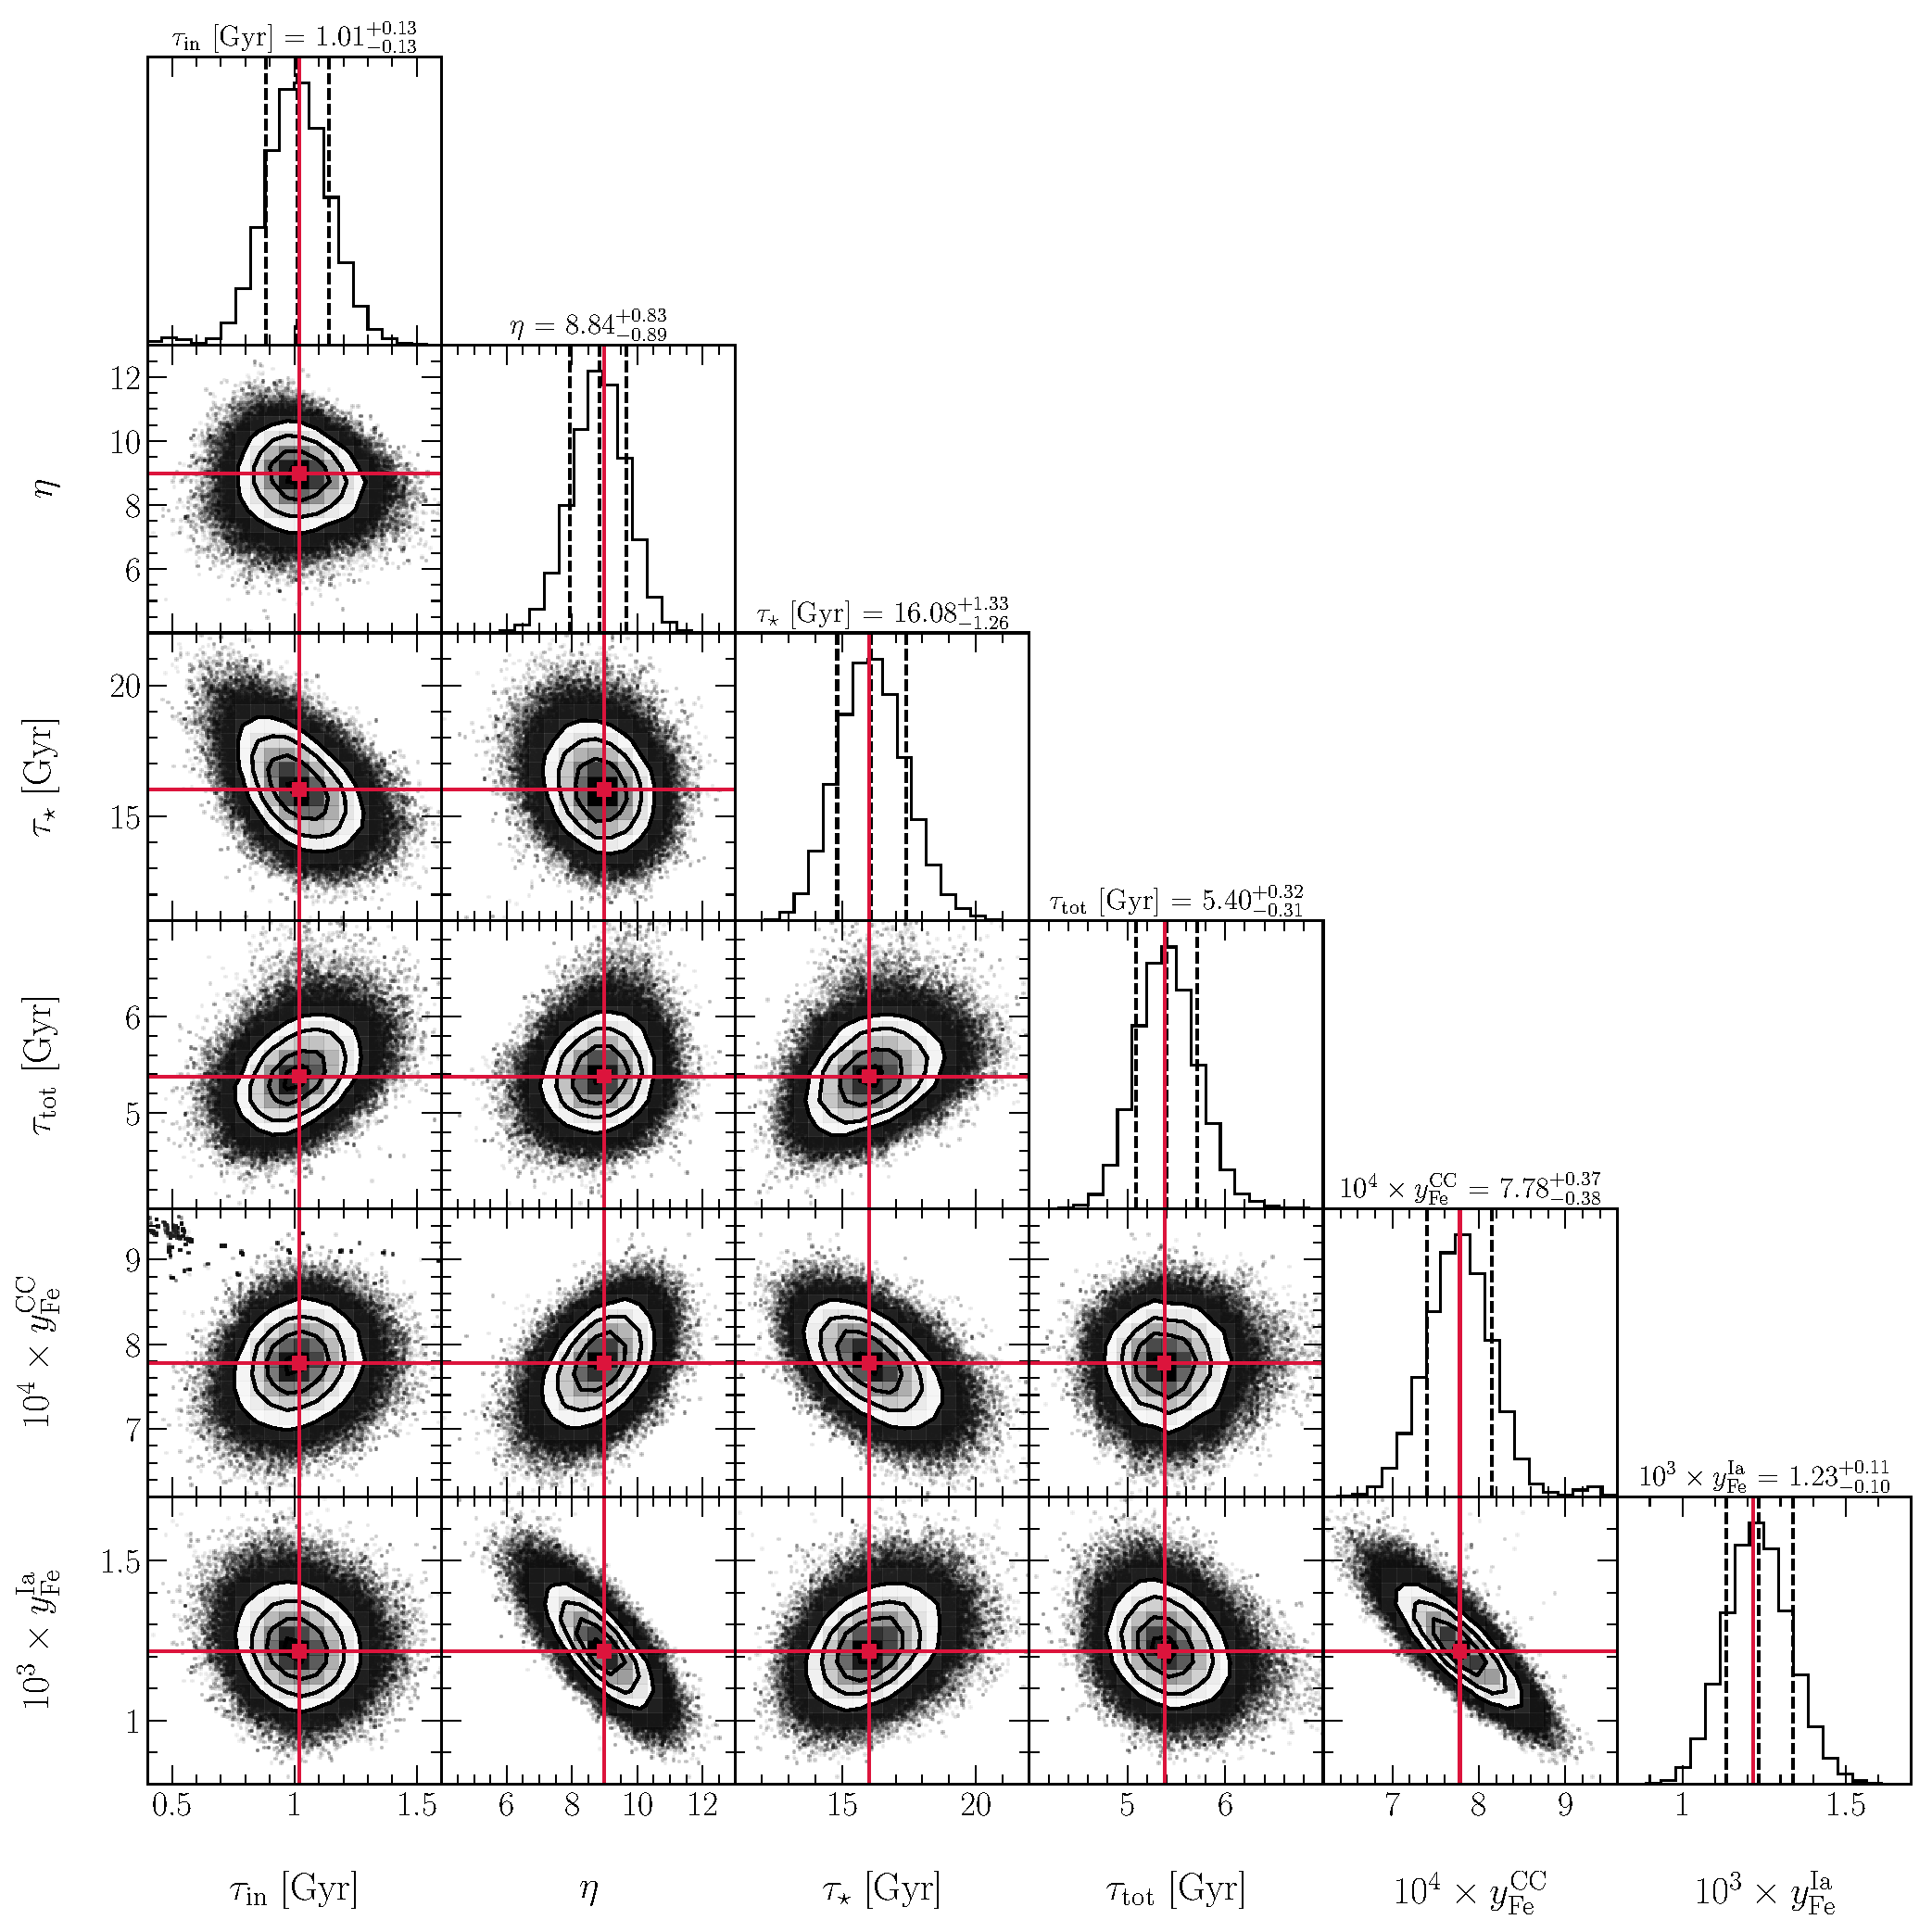
\includegraphics[scale = 0.45]{gsechem_512k.pdf}
\caption{
Posterior distributions for an exponential infall history applied to our GSE
sample.
The parametrization is the same as the input model to our mock samples (see
discussion in~\S~\ref{dga:sec:mocks:fiducial}).
Panels below the diagonal show 2-dimensional cross-sections of the likelihood
function while panels along the diagonal show the marginalized distributions
along with the best-fit values and confidence intervals.
Red ``cross-hairs'' mark the element of the Markov chain with the maximum
statistical likelihood.
The points in the upper left corner of the~$\yfecc - \tau_\text{in}$ plane
are a part of an extended tail of the likelihood distribution which does
not appear in other panels when zoomed in on the peak.
}
\label{dga:fig:gse_corner}
\end{figure*}

% fig 7
\begin{figure}
\centering
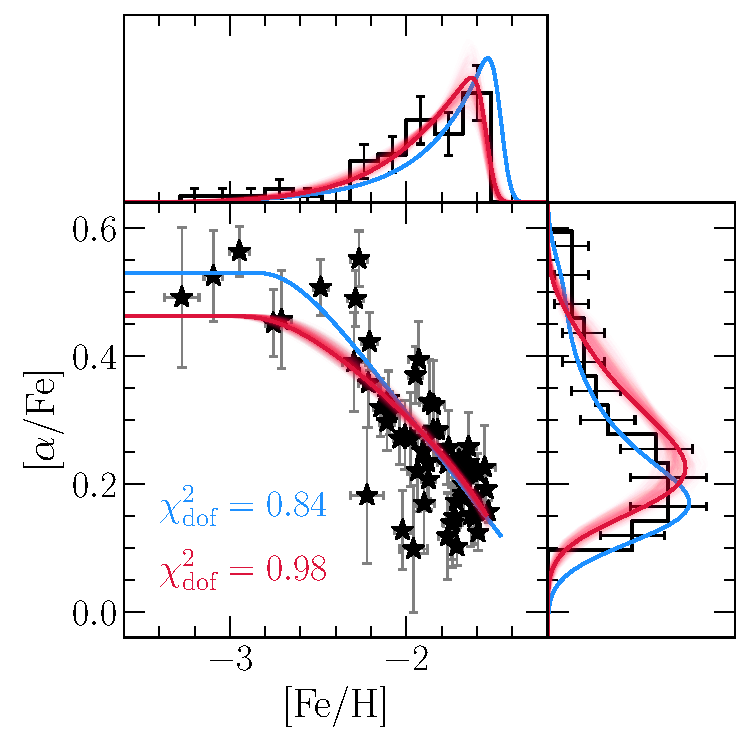
\includegraphics[scale = 0.65]{wukong_bestfit.pdf}
\caption{
Our Wukong/LMS-1 sample in the~\afe-\feh~plane and the associated marginalized
distributions.
Error bars indicate uncertainties on individual abundances in the central panel
and a~$\sigma = \sqrt{N}$ uncertainty from sampling noise in the top and right
panels.
Red lines denote our best-fit chemical evolution model (see discussion
in~\S~\ref{dga:sec:h3:wukong}), with 200 additional sets of parameter choices
subsampled from our Markov chain to give a sense of the fit precision.
Blue lines denote an alternate fit in which we allow the Fe yields to vary as
free parameters.
}
\label{dga:fig:wukong}
\end{figure}

% fig 8
\begin{figure*}
\centering
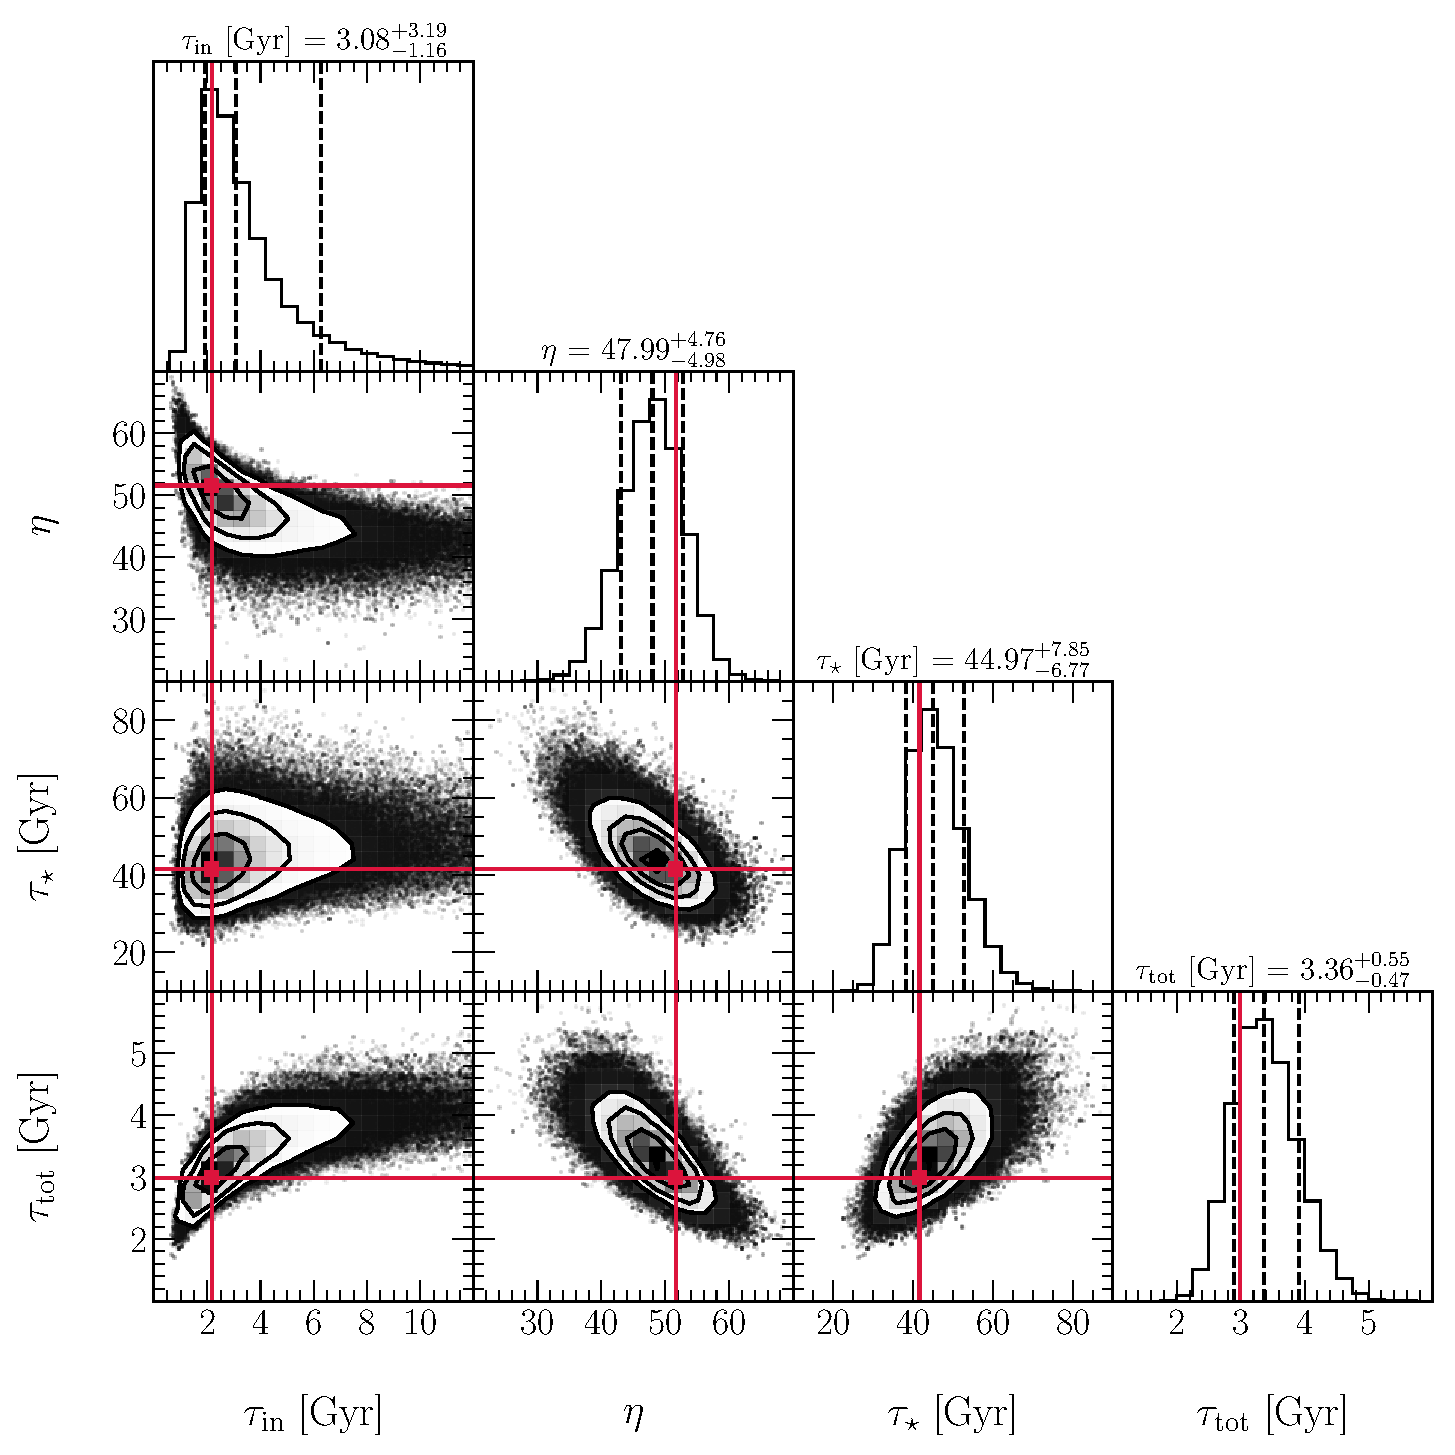
\includegraphics[scale = 0.6]{wukong_512k.pdf}
\caption{
Posterior distributions for an exponential infall history applied to our
Wukong/LMS-1 sample.
The parametrization is the same as the input model to our mock samples (see
discussion in~\S~\ref{dga:sec:mocks:fiducial}) but with the Fe yields held fixed
at the values determined by the fit to our GSE sample
($\yfecc = \scinote{7.78}{-4}$ and~$\yfeia = \scinote{1.23}{-3}$).
Panels below the diagonal show 2-dimensional cross-sections of the likelihood
function while panels along the diagonal show the marginalized distributions
along with the best-fit values and confidence intervals.
Red ``cross-hairs'' mark the element of the Markov chain with the maximum
statistical likelihood.
}
\label{dga:fig:wukong_corner}
\end{figure*}

We select our GSE sample based on the criteria in~\citet{Conroy2022}, which
yields a sample of 189 stars with spectroscopic signal-to-noise
SNR~$> 15$ and~\gaia~RUWE~$< 1.5$.
95 of them are main sequence turnoff and subgiant stars with surface gravities
of~$3.8 < \log g < 4.2$ with reliable age measurements.
Abundance uncertainties range from~$\sim$0.02 to 0.12 dex in
both~\feh~and~\afe~with median values near~$\sim$0.05.
Every age measurement has a statistical uncertainty
$\sigma_{\log_{10}(\text{age})} \leq 0.05$, corresponding to a measurement
precision of~$\lesssim$12\%.
However, due to the difficulty associated with measuring stellar ages both
accurately and precisely~\citep[e.g.,][]{Soderblom2010, Chaplin2013, Angus2019},
we adopt~$0.05$ as the age uncertainty for the entire sample to account for any
systematic errors that may be present.
\par
We illustrate our sample in Fig.~\ref{dga:fig:gse} along with our best-fit GCE
models (see discussion below).
We note the presence of two outliers at ages of~$\sim$5 and~$\sim$6 Gyr, marked
by X's in the right panel of Fig.~\ref{dga:fig:gse}.
With abundances typical of the rest of the GSE population but anomalously young
ages, these stars are likely blue stragglers, which are thought to be made
hotter and more luminous by accretion from a binary companion and biasing their
age measurements to low values~\citep[e.g.,][]{Bond1971, Stryker1993}.
It is also possible that these stars are high-eccentricity contaminants kicked
out of the disk by Sagittarius~\citep[e.g.,][]{Donlon2020}.
The smooth decline of~\afe~with~\feh~and the unimodal nature of the
distributions in~\feh,~\afe~and age indicate that the GSE did not experience
any significant starburst events.
If it had, we would expect to see a multi-peaked age distribution
as well as an increase in~\afe~at a distinct~\feh~due to the perturbed ratio of
CCSN to SN Ia rates~\citep{Johnson2020}.
We therefore fit the GSE with an exponential infall history (the same as our
mock samples explored in~\S~\ref{dga:sec:mocks}), omitting the two~$\sim$5
and~$\sim$6 Gyr old stars from the procedure and retaining the assumption that
star formation commenced 13.2 Gyr ago.
Because H3 selects targets based only on a magnitude range and a maximum
parallax, the selection function in chemical space should be nearly uniform
(i.e.,~$\script{S}(\script{M}_j | \{\theta\}) \approx 1$ for all points
$\script{M}_j$ along the evolutionary track.
We therefore take weights that are proportional to the SFR alone (see
equations~\ref{dga:eq:likelihood} and~\ref{dga:eq:weights} and discussion
in~\S~\ref{dga:sec:fitting}).
\par
We report our best-fit evolutionary parameters in Table~\ref{dga:tab:results}
with Fig.~\ref{dga:fig:gse_corner} illustrating the posterior distributions.
These values suggest strong outflows ($\eta \approx 9$) and inefficient star
formation ($\tau_\star \approx 16$ Gyr).
Invoking the equilibrium arguments of~\citet{Weinberg2017b}, strong outflows and
slow star formation are consistent with the metal-poor mode of the MDF and the
``knee'' in the evolutionary track occurring at low~\feh, respectively.
These results are expected for a dwarf galaxy where the gravity well is
intrinsically shallow and the stellar-to-halo mass ratios are known empirically
to be smaller than their higher mass counterparts~\citep{Hudson2015}.
The alpha-enhanced mode of the MDF reflects the short duration of star
formation, stopping before SN Ia enrichment could produce enough Fe to reach
solar~\afe.
The associated truncation of the age distribution (shown in the bottom left
panel of Fig.~\ref{dga:fig:gse}) likely reflects the quenching of star
formation in the GSE progenitor as a consequence of ram pressure stripping by
the hot halo of the Milky Way after its first infal~$\sim$10 Gyr ago
\citep{Bonaca2020}.
The inferred Fe yields suggest that massive stars account for
$\yfecc / (\yfecc + \yfeia) \approx 40$\% of the Fe in the universe.
These values may however be influenced by the H3 pipeline~\textsc{MINESweeper}
\citep{Cargile2020}, which includes a prior enforcing~$\afe \leq +0.6$ -- if
the~\afe~plateau occurs near this value in nature, this prior could bias the
most alpha-rich stars in our sample to slightly lower~\afe~ratios.
\par
Red lines in Fig.~\ref{dga:fig:gse} illustrate our best-fit model compared to the
data
Visually, this model is a reasonable description of the data, though in detail
it predicts a slightly broader~\feh~distribution and a slightly more peaked age
distribution.
We assess the quality of the fit with equation~\refp{dga:eq:chisquared_dof} and
find~$\chi_\text{dof}^2 = 1.34$, suggesting that this fit is indeed accurate
but that there may be some marginal room for improvement.
The substantial scatter in the age-metallicity relation (lower right panel)
arises due to the age uncertainties -- to clarify this point, we subsample 95
stars (the same number in our sample with age measurements) from our best-fit
SFH and perturb their implied ages and abundances by the median observational
uncertainties.
These random draws (red points) occupy a very similar region of the age-\feh~and
age-\afe~planes.
We do however note an additional~$\sim$6 or 7 potential blue stragglers with
ages of~$\sim$$8 - 9$ Gyr,~$\feh \approx -1.2$ and~$\afe \approx +0.4$.
These stars are less obviously blue stragglers than the~$\sim$5 and~$\sim$6 Gyr
old ones and would not have stood out without this comparison.
These stars likely play a role in increasing the~$\chi_\text{dof}^2$ of our
fit, and removing them from our sample would also bring the observed age
distribution into better agreement with our best-fit model.
We however do not explore more detailed investigations of individual stars for
fits to carefully tailored populations here, and the fit we obtain is
statistically reasonble anyway.
\par
In~\S~\ref{dga:sec:mocks:variations}, we found that our model accurately recovered
the evolutionary timescales of the input model even in the absence of age
information due to their impact on the shape of the MDF.
To assess the feasibility of deducing these parameters from abundances alone,
we conduct an additional fit to our GSE sample omitting the age measurements.
We report the best-fit parameters in Table~\ref{dga:tab:results}.
This procedure results in accurate fits to the~\feh~and~\afe~distributions, and
the SN yields and mass-loading factor~$\eta$ are generally consistent with
and without ages.
The inferred timescales are biased toward higher values and are discrepant
by~$\sim$$2\sigma$, with the duration of star formation showing the largest
difference.
These results indicate that such an approach is theoretically possible, but in
practice age information in some form is essential to pinning down these
timescales.
In~\S~\ref{dga:sec:mocks}, we fit our mock samples with the exact underlying GCE
model and same numerical code which integrated the input model, placing the
same systematic effects in the data as the model.
It is also never guaranteed that the evolutionary history built into the model
is an accurate description of the galaxy.
% While the most powerful way to provide age information for a fit under this
% procedure is with star-by-star measurements, that is difficult for external
% galaxies with current instrumentation and could instead be achieved with, e.g.,
% a CMD-derived SFH included as a prior.

\subsection{Wukong/LMS-1}
\label{dga:sec:h3:wukong}

% fig 9
\begin{figure}
\centering
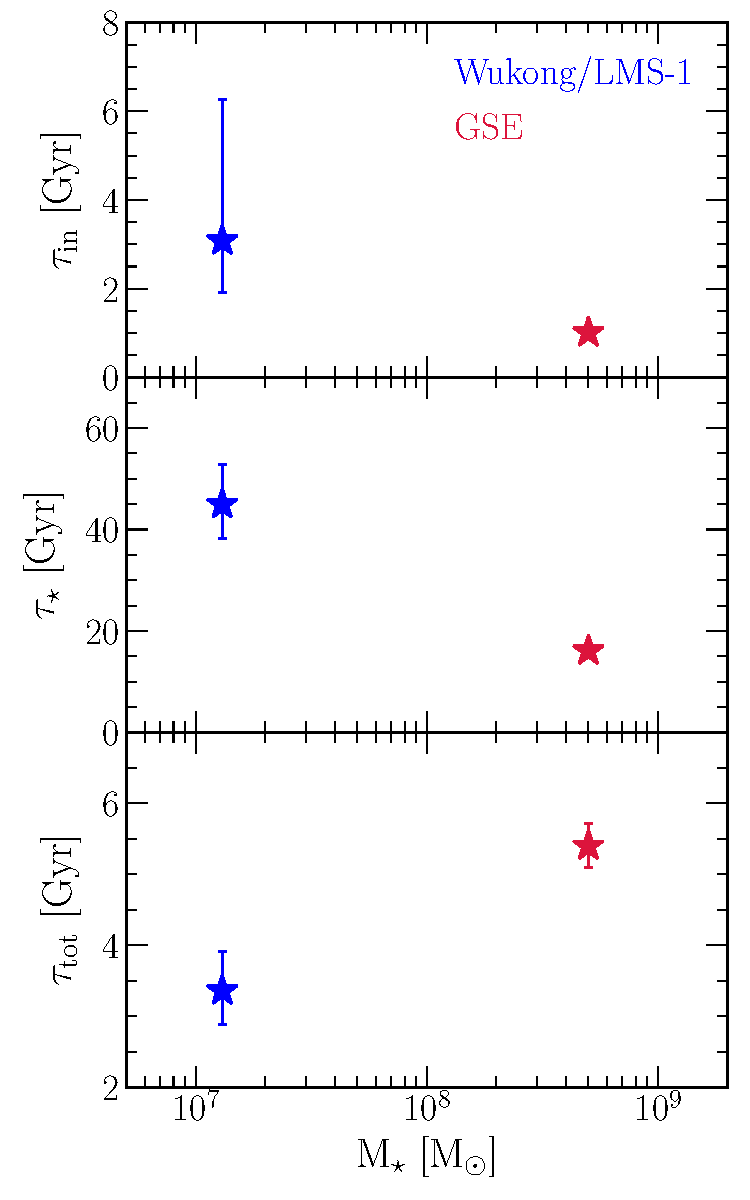
\includegraphics[scale = 0.63]{gse_wukong_timescales.pdf}
\caption{
Our best-fit evolutionary timescales for Wukong/LMS-1 (blue) and GSE (red) as a
function of their stellar mass (taken from~\citealt{Naidu2022}; values are
tabulated in Table~\ref{dga:tab:results}).
The uncertainties in the infall timescale~$\tau_\text{in}$ and the SFE
timescales~$\tau_\star$ for GSE are smaller than the point.
}
\label{dga:fig:gse_wukong_timescales}
\end{figure}

% fig 10
\begin{figure}
\centering
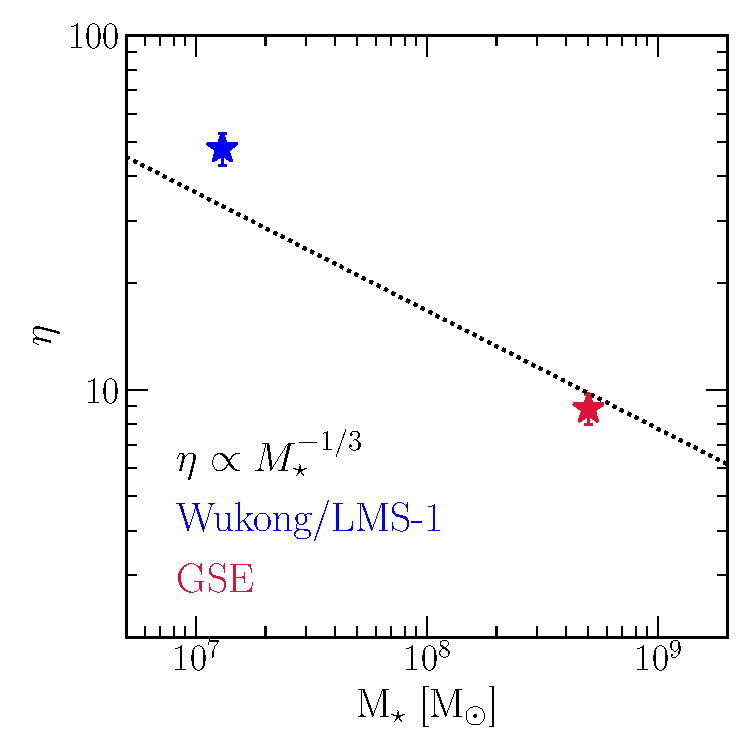
\includegraphics[scale = 0.6]{gse_wukong_eta.pdf}
\caption{
Our best-fit mass-loading factors~$\eta$ for Wukong/LMS-1 (blue) and GSE (red) as
a function of their stellar mass (taken from~\citealt{Naidu2022}; values are
tabulated in Table~\ref{dga:tab:results}).
The black dashed line denotes~$\eta \propto M_\star^{-1/3}$ as suggested by
\citet{Finlator2008} and~\citet{Peeples2011} with the normalization of
$\eta = 3.6$ at~$M_\star = 10^{10}~M_\odot$ taken from~\citet{Muratov2015}.
}
\label{dga:fig:gse_wukong_eta}
\end{figure}

We select Wukong/LMS-1 stars following the criteria in~\citet{Naidu2020}, with
the following additional cuts for high purity (inspired by the orbits of the
accomparnying globular clusters, NGC 5024 and NGC 5053, and~\citealt{Yuan2020}
and~\citealt{Malhan2021} who made selections based on the orbital plane):
\begin{itemize}

	\item[\textbf{1.}] $(J_z - J_r) / J_\text{tot}$ > 0.7, where~$J$ is action.

	\item[\textbf{2.}] $90^\circ < \theta < 120^\circ$, where~$\theta$ and
	$\phi$ are angles defining the angular momentum unit vector.

\end{itemize}
The~\citet{Naidu2020} selection features a hard cut at~$\feh < -1.45$ to avoid
GSE contamination, but visual inspection of the Wukong/LMS-1 sequence in
the~\afe-\feh~plane indicates that it drops off around~$\feh \approx -1.5$,
(see Fig.~\ref{dga:fig:wukong}) and high [$\alpha$/Fe] GSE stars appear at higher
metallicities.
Our sample consists of 57 stars with spectroscopic SNR~$> 10$
and~\gaia~RUWE~$< 1.5$, none of which have age information as they are all
distant halo stars.
Within this sample, 23 stars are at SNR~$> 20$ and the remaining 34 are at
$10 <$ SNR~$< 20$.
Abundance uncertainties range from~$\sim$0.02 to~$\sim$0.10 dex in
both~\afe~and~\feh~with median values near~$\sim$0.045.
\par
Fig.~\ref{dga:fig:wukong} illustrates this sample in chemical space along with our
best-fit GCE model (see discussion below).
Similar to the GSE, the lack of discontinuities in the age and abundance trends
indicates a smooth SFH devoid of any starburst events.
We therefore fit this sample with the same exponential infall history as the
input model to our mock samples, which we also applied to our GSE data.
We retain the assumption that star formation began 13.2 Gyr ago and that the H3
selection function is uniform in chemical space (see discussion
in~\S~\ref{dga:sec:h3:gse}).
However, due to the smaller sample size and the lack of age information, we
initially hold our Fe yields fixed at~$\yfecc = \scinote{7.78}{-3}$ and
$\yfeia = \scinote{1.23}{-3}$ as suggested by the fit to our GSE sample.
It is reasonable to expect SN yields to be the same from galaxy-to-galaxy since
they are set by stellar as opposed to galactic physics, though we explore the
impact of relaxing this assumption below.
\par
Table~\ref{dga:tab:results} reports the inferred best-fit parameters and
Fig.~\ref{dga:fig:wukong_corner} illustrates the posterior distributions.
The degeneracies between parameters are noticeably more asymmetric than in our
GSE sample, a result of the lack of age information (we found similar effects
in our tests against mock data in~\S~\ref{dga:sec:mocks}, though we did not discuss
it there).
The e-folding timescale of the accretion rate in particular has a highly skewed
likelihood distribution ($\tau_\text{in} = 3.08^{+3.19}_{-1.16}$ Gyr).
We have also had reasonable success describing Wukong/LMS-1 with a constant
star formation history.
Consequently, the likelihood function has a tail that extends
to~$\tau_\text{in} \rightarrow \infty$.
The exponential infall history is indeed a statistically better fit, so
throughout this section we include a prior that
enforces~$\tau_\text{in} \leq 50$ Gyr to focus on this portion of parameter
space.
This tail is significantly more extended if the Fe yields are allowed to vary
as a free parameter (see Table~\ref{dga:tab:results} and discussion below).
\par
An exponential infall history yields a statistically good fit
($\chi_\text{dof}^2 = 0.98$; equation~\ref{dga:eq:chisquared_dof}) for Wukong/LMS-1,
though visually it appears that the SN yields implied by our GSE data
underestimate the height of the [$\alpha$/Fe] plateau, which we indirectly
held fixed via the Fe yields.
Although we asserted above that it is reasonable expect SN yields to be the
same between Wukong/LMS-1 and GSE, variations in the plateau height could
indicate either metallicity-dependent yields or variations in the IMF.
To investigate this hypothesis, we conduct an additional fit where we allow
the Fe yields to vary as free parameters, reporting the results in
Table~\ref{dga:tab:results} and illustrating the deduced model for comparison in
Fig.~\ref{dga:fig:wukong}.
A higher plateau indeed provides an even better fit
($\chi_\text{dof}^2 = 0.84$), but with~$\chi_\text{dof}^2$ less than 1, this
could be an overparametrization of the data.
This possibility is not necessarily to a worrisome extent though; we cannot
rule out either model.
The best-fit SFE timescales between the two fits are in excellent agreement,
indicating that~$\tau_\star$ does not significantly impact the height of the
plateau (to first-order, it determines the position of the knee in the
track;~\citealp{Weinberg2017b}).

\subsection{Comparison}
\label{dga:sec:h3:comparison}

Fig.~\ref{dga:fig:gse_wukong_timescales} compares the best-fit evolutionary
timescales between GSE and Wukong/LMS-1 as a function of their stellar mass (we
adopt the stellar masses inferred by~\citealt{Naidu2021, Naidu2022}; our GCE
models as we have parametrized them do not offer any constraints on this
quantity).
Due to the yield-outflow degeneracy (see Appendix~\ref{dga:sec:degeneracy}), only
relative values of~$\tau_\star$ carry meaning, while the absolute values of
$\tau_\text{in}$ and~$\tau_\text{tot}$ do.
Qualitatively consistent with semi-analytic models of galaxy formation
\citep[e.g.,][]{Baugh2006, Somerville2015a, Behroozi2019} and results from
hydrodynamical simulations~\citep[e.g.,][]{GarrisonKimmel2019}, the less
massive of the two galaxies experienced the more extended accretion history.
Star formation in Wukong/LMS-1, however, was less efficient and did not last as
long as in GSE -- sensible results given the empirical correlation between
stellar-to-halo mass ratioes and stellar mass~\citep{Hudson2015}.
To the extent that our one-zone model framework is accurate, we have
constrained the duration of star formation in Wukong/LMS-1 and GSE to 15.2\%
and 5.8\%, respectively.
However, our Wukong/LMS-1 sample has no age measurements, and we have not
derived an SFH from its CMD here.
The failure of our fit to GSE omitting all ages (see Table~\ref{dga:tab:results})
suggests that these best-fit parameters may be biased to high values.
\par
As expected given Wukong/LMS-1's shallower gravity well, it experienced
stronger mass-loading than GSE.
Fig.~\ref{dga:fig:gse_wukong_eta} shows the inferred mass-loading factors in
comparison to the scaling of~$\eta \propto M_\star^{-1/3}$ as suggested by
\citet{Finlator2008} and~\citet{Peeples2011} modelling the impact of galactic
winds on the mass-metallicity realtion for galaxies.
We take the normalization of~$\eta = 3.6$ at~$M_\star = 10^{10}~M_\odot$ from
\citet{Muratov2015} who find a similar scaling in the FIRE simulations
($\eta \propto M_\star^{-0.35}$;~\citealp{Hopkins2014}).
There is excellent agreement between this predicted scaling and our one-zone
model fits -- rather remarkably so given that we have made no deliberate
choices for either the normalization or the slope to agree.
\par
In Fig.~\ref{dga:fig:comparison}, we compare our best-fit models for GSE and
Wukong/LMS-1.
The intrinsic age distribution of GSE is predicted with considerably higher
precision than for Wukong/LMS-1, a consequence of the lack of age information
in our Wukong/LMS-1 sample.
The uncertainties in the Wukong/LMS-1 age distribution are noticeably
asymmetric due to the skewed posterior distribution of the infall timescale
($\tau_\text{in} = 3.08^{+3.19}_{-1.16}$ Gyr).
If our assumption that star formation began~$T \approx 13.2$ Gyr ago (see
discussion in~\S~\ref{dga:sec:mocks:fiducial}) is accurate for Wukong/LMS-1, then
it experienced quenching~$\sim$2 Gyr earlier than the GSE ($\sim$9.8 versus
$\sim$7.8 Gyr ago).
However, because we do not have age information for Wukong/LMS-1, this
distribution could shift uniformly to lower values with affecting the quality
of the fit.
Constraints on the centroid of the distribution could be derived by
analysing the CMD as in, e.g.,~\citet{Dolphin2002} and~\citet{Weisz2014b}, but
we do not pursue this method in the present paper as it involves an entirely
separate mathematical framework.
\par
Also as a consequence of the lack of age information, our fits constrain the
intrinsic age-\feh~and age-\afe~relations to somewhat higher precision for GSE
than Wukong/LMS-1.
While the age-\feh~relations are significantly offset from one another, the
predicted age-\afe~relations are remarkably consistent with one another.
A portion of this agreement can likely be traced back to our fixing the Fe
yields in our fit to Wukong/LMS-1 to the values inferred in our fit to GSE.
Nonetheless, it is reasonable to assume that the SN yields are the same between
the two galaxies because this should be set by stellar physics, sufficiently
decoupled from the galactic environment.
The evolution of~\afe~with time is in principle impacted by the various
evolutionary timescales at play, so their consistency with one another is still
noteworthy.



\section{Discussion and Conclusions}
\label{dga:sec:conclusions}

% fig 11
\begin{figure*}
\centering
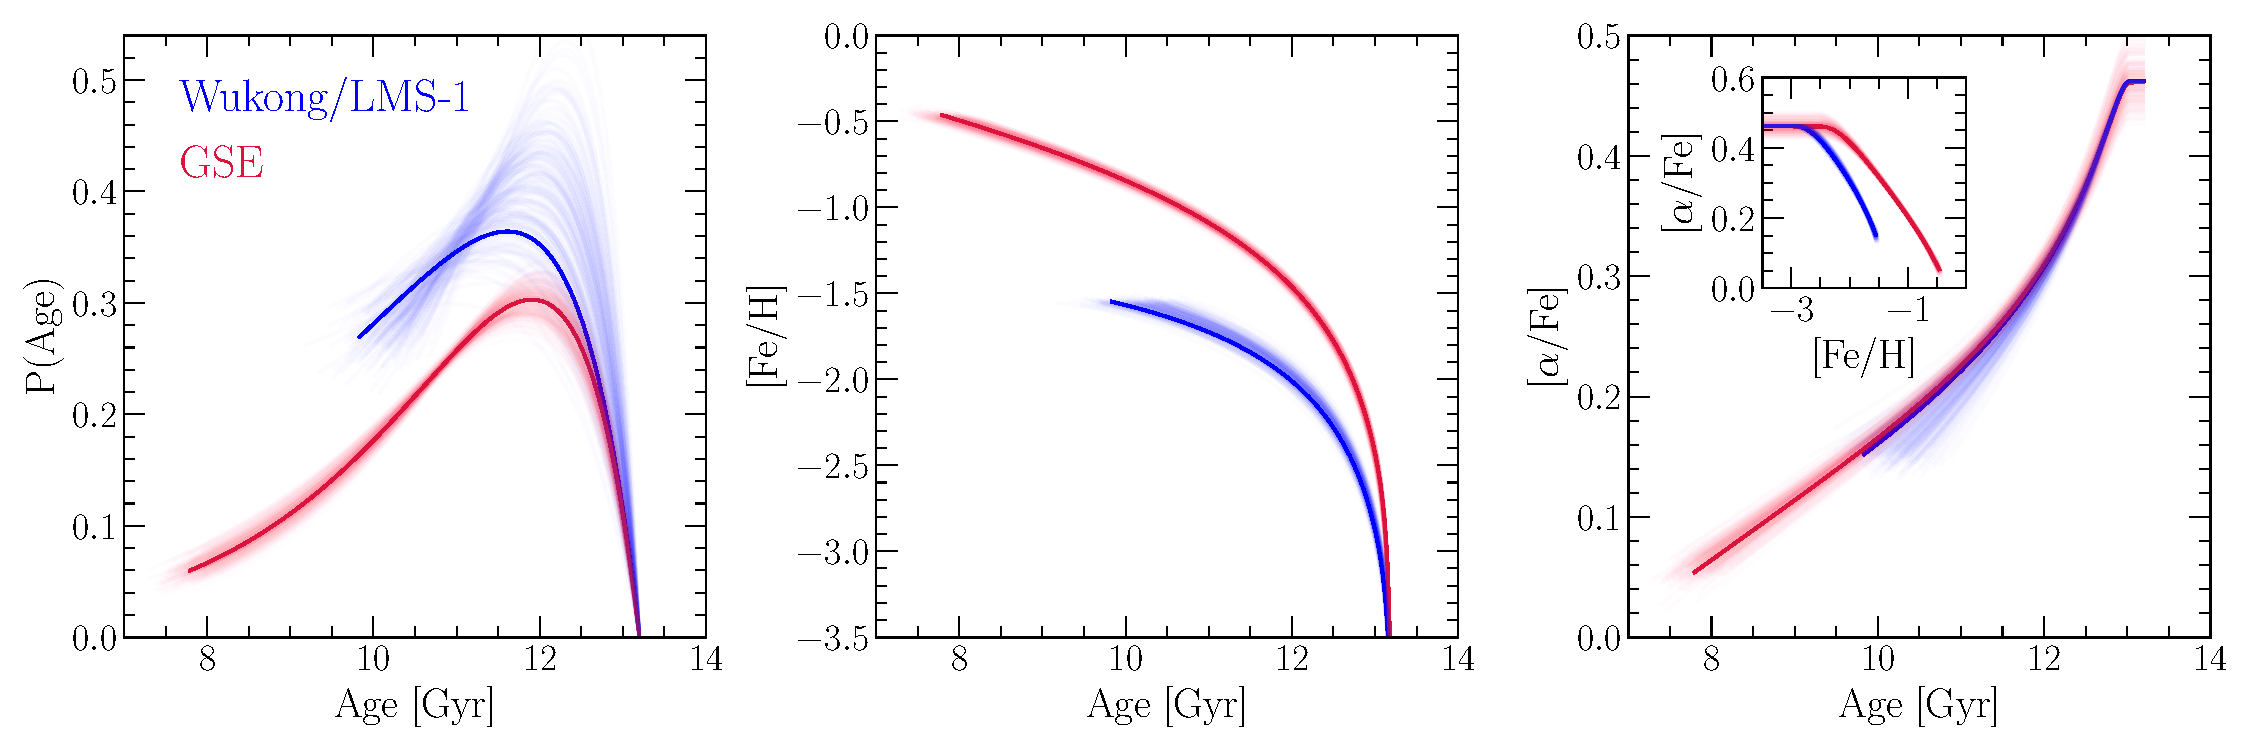
\includegraphics[scale = 0.45]{gse_wukong_comparison.pdf}
\caption{
A comparison of our best-fit models for GSE (red) and Wukong/LMS-1 (blue): the
age distributions (left), the age-\feh~relations (middle) and age-\afe~relations
(right).
The inset in the right hand panel shows the tracks in the~\afe-\feh~plane.
In all panels, we subsample 200 additional parameter choices from our Markov
chains and plot the predictions as high transparency lines to provide a sense
of the fit uncertainty.
Due to the lack of age information for Wukong/LMS-1, the centroid of the age
distribution is determined by our assumption that star formation began 13.2
Gyr ago (see discussion in~\S~\ref{dga:sec:mocks:fiducial}).
}
\label{dga:fig:comparison}
\end{figure*}

We use statistically robust methods to derive best-fit parameters of
one-zone GCE models for two disrupted dwarf galaxies in the Mily Way stellar
halo: GSE~\citep{Belokurov2018, Helmi2018}, and Wukong/LMS-1~\citep{Naidu2020,
Naidu2022, Yuan2020}.
We fit both galaxies with an exponential accretion history
(see~\S~\ref{dga:sec:mocks}), deriving e-folding timescales and durations of star
formation of~$(\tau_\text{in}, \tau_\text{tot}) \approx (1~\text{Gyr},
5.4~\text{Gyr})$ for GSE and~$(\tau_\text{in}, \tau_\text{tot}) \approx
(3.1~\text{Gyr}, 3.4~\text{Gyr})$ for Wukong/LMS-1 (we refer to table
\ref{dga:tab:results} for exact values).
These differences in evolutionary parameters are qualitatively consistent with
predictions from hydrodynamical simulations~\citep[e.g.,][]{GarrisonKimmel2019}
and semi-analytic models of galaxy formation~\citep[e.g.,][]{Baugh2006,
Somerville2015a, Behroozi2019}.
\par
Quantitatively, we arrive at a longer duration of star formation than
\citet{Gallart2019}, who derived an age distribution for GSE by analysing its
CMD according to the method described in~\citet{Dolphin2002} and found a
median age of 12.37 Gyr.
Consistent with their results,~\citet{Vincenzo2019b} infer a sharply declining
infall history with a timescale of~$\tau_\text{in} = 0.24$ Gyr.
However, the star-by-star age measurements provided by H3~\citep{Conroy2019}
suggest that GSE's SFH was more extended (see Fig.~\ref{dga:fig:gse}).
The peak of the age distribution is near~$\sim$11 Gyr (Fig.~\ref{dga:fig:gse}),
consistent with Feuillet et al.'s~\citeyearpar{Feuillet2021} results
from~\gaia~\citep{GaiaCollaboration2016} and APOGEE~\citep{Majewski2017}.
Consequently, we deduce a higher value of~$\tau_\text{in}$ of~$1.01 \pm 0.13$
Gyr.
If its first infall into the Milky Way halo was~$\sim$10 Gyr ago
\citep[e.g.,][]{Helmi2018, Bonaca2020}, then depending on exactly how long ago
it started forming stars, the duration of star formation we derive
($\tau_\text{tot} = 5.4$ Gyr) implies that GSE formed stars for~$\sim$$1.5 - 2$
Gyr after its first infall.
\par
To our knowledge, this is the first detailed modelling of multi-element stellar
abundances in Wukong/LMS-1.
Wukong/LMS-1 experienced a more extended accretion history
($\tau_\text{in} = 3.08^{+3.19}_{-1.16}$ Gyr), but the duration of star
formation was~$\sim$2 Gyr shorter than in GSe.
If they started forming stars around the same time, then Wukong/LMS-1 was
quenched at approximately the time of GSE's first infall.
However, our sample includes no age information for Wukong/LMS-1, so the
centroid of the age distribution is a prediction of our model as opposed to an
empirical constraint.
We find no statistically significant evidence of IMF variability or
metallicity-dependent Fe yields comparing GSE and Wukong/LMS-1.
A pathway to investigate this hypothesis further and potentially pin down the
yield-outflow degeneracy as well (see discussion in
Appendix~\ref{dga:sec:degeneracy}) is to perform a hierarchical analysis of a
sample of galaxies where the yields are free parameters but are required to be
the same for all systems.
\par
Although these models are statistically good descriptions of our GSE and
Wukong/LMS-1 data, they are simplified in nature.
In particular, we have assumed a linear relation between the gas supply and the
SFR while empirical results would suggest a non-linear relation
\citep[e.g.,][]{Kennicutt1998, Kennicutt2012, delosReyes2019, Kennicutt2021}.
We have also taken a constant outflow mass-loading factor~$\eta$, when in
principle this parameter could vary with time as the potential well of the
galaxy deepens as in, e.g.,~\citet{Conroy2022}.
The primary motivation of these choices, however, is to provide proof of
concept for our fitting method with an example application to observations.
We reserve more detailed modelling of galaxies with both simple and complex
evolutionary histories for future work.
\par
Our method is built around a likelihood function which requires no binning of
the data (Eq.~\ref{dga:eq:likelihood}) and has two central features.
First, the likelihood of observing some datum~$\script{D}_i$ must be
marginalized over the entire evolutionary track~\script{M}.
This requirement arises due to measurement uncertainties: for any given datum,
it is impossible to know where on the track the observation truly arose from,
and mathematically accounting for this requires considering all pair-wise
combinations between~\script{M} and~\script{D}.
Second, the likelihood of observing a datum~$\script{D}_i$ given a point on
the evolutionary track~$\script{M}_j$ must be weighted by the SFR at that time
in the model, simultaneously folding in any selection effects introduced by the
survey.
This requirement arises because an observed star is proportionally more likely
to have been sampled from an epoch of a galaxy's history in which the SFR was
large and/or if the survey designed is biased toward certain epochs.
\par
We establish the accuracy of our method by means of tests against mock data,
demonstrating that the known evolutionary parameters of subsampled input models
are accurately re-derived across a broad range of sample sizes
($N = 20 - 2000$), abundance uncertainties ($\sigma_\text{[X/Y]} = 0.01 - 0.5$),
age uncertainties ($\sigma_{\log_{10}(\text{age})} = 0.02 - 1$) and the
fraction of the sample with age information ($f_\text{age} = 0 - 1$; see
discussion in~\S~\ref{dga:sec:mocks}).
The fit precision of the inferred parameters generally scales with sample size
as~$\sim$$N^{-0.5}$.
We demonstrate that evolutionary timescales can theoretically be derived with
abundances alone, but in practice age information helps reduce the effect of
systematic differences between the data and model, improving both the
accuracy and the precision.
Our likelihood function requires no binning of the data, and we derive it
in Appendix~\ref{dga:sec:likelihood} assuming only that the model predicts an
evolutionary track of some unknown shape in the observed space.
It should therefore be applicable to one-zone models of any parametrization as
well as easily extensible to other astrophysical models in which the chief
prediction is a track of some form (e.g., stellar streams and isochrones).
\par
Having provided proof of concept for our method, a promising direction for
future work is to apply it to a much broader sample of disrupted dwarf galaxies
in the Milky Way stellar halo to take a ``chemical census'' of the accreted
systems.
This approach is also of interest to authors seeking to derive quenching
times (i.e., the lookback time to when star formation stopped) for intact and 
disrupted dwarf galaxies.
At present, the most reliable method to empirically determine a dwarf galaxy's
quenching time is via a direct reconstruction of its SFH through some method,
such as analysing its CMD~\citep[e.g.,][]{Dolphin2002, Weisz2015}.
Consequently, the most precise SFH measurements are for nearby systems with
resolved stars, a considerable limitation even with modern instrumentation.
To our knowledge, there are only four quenched galaxies outside of the Milky
Way subgroup with well-constrained SFHs: Andromeda II, Andromeda XIV
\citep{Weisz2014a}, Cetus~\citep{Monelli2010a} and Tucana~\citep{Monelli2010b}.
Some authors have connected quenching timescales to observed galaxy properties
in N-body simulations (e.g.,~\citealp*{Rocha2012};~\citealp{Slater2013,
Slater2014, Phillips2014, Phillips2015, Wheeler2014}), but unfortunately
simulation outcomes are strongly dependent on the details of the adopted
sub-grid models~\citep[e.g.,][]{Li2020} as well as how feedback and the grid
itself are implemented~\citep{Hu2022}.
Our results suggest that chemical abundances can provide valuable additional
information for these methods.
% Our results suggest that the duration of star formation can instead be inferred
% from elemental abundance alone, though having~\textit{some} age information can
% significantly improve the precision of the fit.
% While this is theoretically possible, we demonstrate in~\S~\ref{dga:sec:h3:gse}
% below that the exclusion of age information from the fit to our GSE sample
% produces significantly different results for evolutionary timescales.
% These discrepancies indicate that age information in some form is more
% important in practice than our proof of concept would suggest.
\par
% This method could have a strong impact in deriving SFHs and quenching times for
% dwarf galaxies.
However, with current instrumentation, spectroscopic measurements of
multi-element abundances in dwarf galaxies are limited to the local group
\citep[e.g.,][]{Kirby2011, Kirby2020}, and sample sizes are small even for
these relatively nearby systems.
Larger sample sizes could potentially be achieved with a high
angular resolution integral field unit such as the Multi Unit Spectroscopic
Explorer~\citep[MUSE;][]{Bacon2014}.
Alternatively, photometry is more conducive to larger sample sizes due to the
lower observational overhead, and the MDF can still be constrained using the
CMD~\citep[e.g.,][]{Lianou2011}.
One possibility is to forward-model the CMDs of dwarf galaxies using the SFHs
and MDFs predicted by one-zone GCE models, simultaneously constraining both
quantities photometrically.
% In some cases, narrow-band imaging can also provide worthwhile constraints on
% the MDF~\citep{Fu2022}, particularly when combined with machine learning
% algorithms trained on spectroscopic data~\citep{Whitten2011}.
The high angular resolution of the James Webb Space Telescope
\citep[JWST;][]{Gardner2006} should provide a considerable increase in the
number of resolved stars in nearby galaxies, making it a promising instrument
to pursue this potential pathway.
Farther in the future, the upcoming Nancy Grace Roman Space Telescope
(\citealp{Spergel2013, Spergel2015}; formerly WFIRST) will revolutionize
stellar populations in nearby galaxies.
In the era of next-generation telescopes, statistically robust methods such as
the one detailed in this paper will be essential to deduce the lessons the
community can learn about dwarf galaxy evolution.



\end{document}


% 
\documentclass[main.tex]{subfiles}
\begin{document}

\chapter{Binaries Drive High Type Ia Supernova Rates in Dwarf Galaxies}
\label{iarates}


\begin{center}
\textit{
	The results presented in this chapter are part of a first-author paper
	submitted to Monthly Notices of the Royal Astronomical Society, in which I
	led the majority of the analysis and writing.
}
\end{center}

\section{Introduction}
\label{iarates:sec:intro}
Type Ia supernovae (SNe Ia) arise from the thermonuclear detonation of a white
dwarf~\citep[WD;][]{Hoyle1960, Colgate1969}, the exposed carbon-oxygen core of
a low-mass star.
SN surveys have revealed that low-mass galaxies are more efficient producers
of these events than their higher mass counterparts~\citep[e.g.,][]{Mannucci2005,
Sullivan2006, Li2011, Smith2012}.
In particular,~\citet{Brown2019} found that the specific SN Ia rate -- the rate
per unit stellar mass -- scales approximately with the inverse square root of
the stellar mass itself ($\dot{\text{N}}_\text{Ia} / \mstar \sim \mstar^{-0.5}$)
using SNe Ia from the All-Sky Automated Survey for Supernovae
\citep[ASAS-SN;][]{Shappee2014, Kochanek2017} and assuming the~\citet{Bell2003}
stellar mass function (SMF).
The measurement depends on the SMF because the number of
observed SNe must be normalized by the number of galaxies in order to compute a
specific SN rate.
Consequently, the scaling becomes shallower ($\dot{\text{N}}_\text{Ia} / \mstar
\sim \mstar^{-0.3}$) when using the steeper~\citet{Baldry2012} double-Schechter
SMF parametrization~\citep{Gandhi2022}.
This change leads to agreement between the ASAS-SN measurements and Wiseman et
al.'s~\citeyearpar{Wiseman2021} estimates from the Dark Energy
Survey~\citep[DES;][]{DarkEnergySurveyCollaboration2016} using
the~\citet{Baldry2012} SMF.
Although the exact strength of the scaling depends on the SMF, it is clear
that the specific SN Ia rate is higher in dwarf galaxies.
There are a handful of potential pathways which could give rise to this
empirical result.
\par
First, the mean star formation histories (SFHs) of galaxies vary with the
stellar mass of the system.
In semi-analytic models of galaxy formation (see, e.g., the reviews of
\citealt{Baugh2006} and~\citealt{Somerville2015a}), dwarf galaxies in the field
have more extended SFHs than their higher mass counterparts.
This mass dependence is also seen in hydrodynamical simulations of galaxy
formation~\citep[e.g.,][]{GarrisonKimmel2019}.
Since SN Ia delay-time distributions (DTDs) decline with age, galaxies with
more recent star formation should have higher specific SN Ia rates.
\par
Second,~\citet{Kistler2013} argued that the dependence of the specific SN Ia
rate on stellar mass may be driven by metallicity.
Lower mass galaxies host lower metallicity stellar populations
\citep{Gallazzi2005, Kirby2013} and lower metallicity gas reservoirs
(\citealp{Tremonti2004};~\citealp*{Zahid2011};~\citealp{Andrews2013,
Zahid2014}).
\citet{Kistler2013} point out that lower metallicity stars leave behind higher
mass WDs which could potentially grow to the Chandrasekhar mass and
subsequently explode more easily than their less massive, high metallicity
counterparts.
Lower metallicity stars have weaker winds during the asymptotic giant branch
phase~\citep{Willson2000, Marigo2007}, leading to lower mass loss rates and
more massive cores~\citep{Kalirai2014}, producing more massive WDs for fixed
initial mass stars at lower metallcity (\citealp{Umeda1999};
\citealp*{Meng2008};~\citealp{Zhao2012}).
\par
Furthermore, in both the single~\citep[e.g.,][]{Whelan1973} and double
degenerate scenarios (e.g.,~\mbox{\citealp{Iben1984}};
\mbox{\citealp{Webbink1984}}), SNe Ia arise in binary systems.
Based on multiplicity measurements of Solar-type stars from the Apache Point
Observatory Galaxy Evolution Experiment~\citep[APOGEE;][]{Majewski2017},
\citet{Badenes2018} and~\citet*{Moe2019} find that the stellar close binary
fraction increases toward low metallicities.
% in APOGEE\footnote{
% 	Apache Point Observatory Galaxy Evolution Experiment
% }~\citep{Majewski2017},~\citet*{Moe2019} found that the stellar close binary
% fraction increases from~$\sim$10\% at~$\sim$$3Z_\odot$ where~$Z_\odot$ is the
% Solar metallicity to~$\sim$40\% at~$\sim$$0.1 Z_\odot$.
Consequently, dwarf galaxies should have more potential SN Ia progenitors per
unit mass of star formation due to more massive WDs and a higher close binary
fraction.
Motivated by these results,~\citet{Gandhi2022} explore a handful of
parametrizations for the metallicity dependence of the SN Ia rate in
re-simulated galaxies from FIRE-2~\citep{Hopkins2018}.
They find that a~$Z^{-0.5}$ scaling where~$Z$ is the metallicity leads
to better agreement with the empirical relationship between galactic stellar
masses and stellar abundances than when using metallicity-independent SN Ia
rates.
\par
In this paper, we assume that the strong scaling of the specific SN Ia rate
with stellar mass is due to metallicity and conduct simple numerical
calculations to investigate its origin.
We combine the mean star formation histories of galaxies at fixed stellar
mass from the~\um~semi-analytic model~\citep{Behroozi2019} and the popular
$\tau^{-1}$ SN Ia DTD~\citep[e.g.,][]{Maoz2012a} with the mass-metallicity
relation (MZR) for galaxies~\citep{Tremonti2004, Andrews2013, Zahid2011,
Zahid2014}.
Given the mean SFH and DTD, we can compute the characteristic SN Ia rate for
galaxies of a given stellar mass, and by assuming that they lie along the
observed MZR, we can include various scalings of the rate with metallicity.
We describe the model in~\S~\ref{iarates:sec:galprops} and the effect on Type Ia rates
in~\S~\ref{iarates:sec:predictions}.
In~\S~\ref{iarates:sec:gce} we present simple models exploring the consequences of
metallicity-dependent SN Ia rates for galactic chemical evolution models.
We summarize our findings in~\S~\ref{iarates:sec:conclusions}.



\section{Galactic Properties}
\label{iarates:sec:galprops}

% fig 1
\afterpage{
\clearpage
\begin{landscape}
\begin{figure*}
\centering
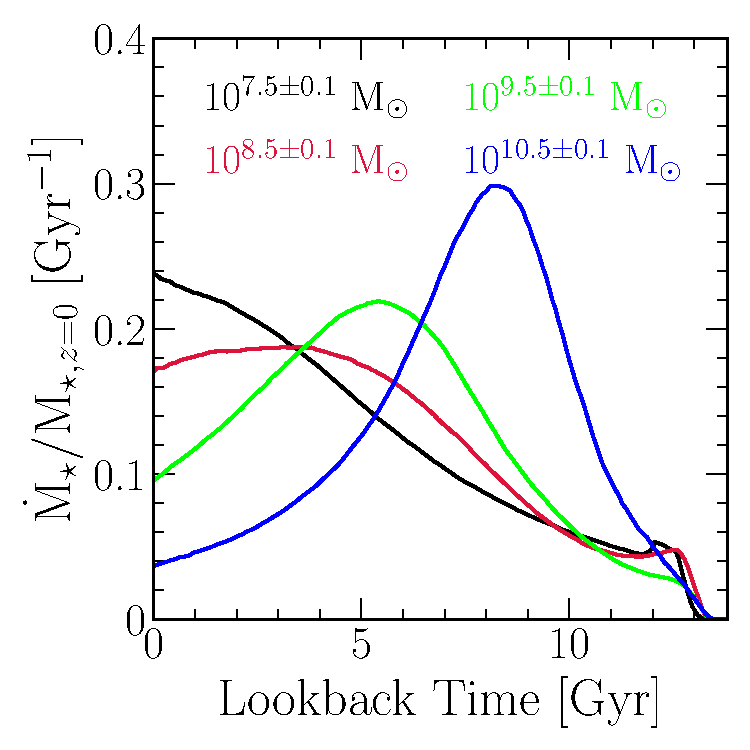
\includegraphics[scale = 0.51]{umachine_sfhs.pdf}
\includegraphics[scale = 0.5]{iarate_vs_tausfh.pdf}
\includegraphics[scale = 0.5]{mzr.pdf}
\caption{
\textbf{Left}: The best-fit mean SFHs of the~\um~galaxies with present-day
stellar masses of $\mstar = 10^{7.5 \pm 0.1}$ (black),~$10^{8.5 \pm 0.1}$ (red),
$10^{9.5 \pm 0.1}$ (green), and $10^{10.5 \pm 0.1} \msun$ (blue) normalized by
their present-day stellar masses.
\textbf{Middle}: The specific SN Ia rate as a function of the e-folding
timescale of the SFH~$\tau_\text{sfh}$ assuming a linear-exponential time
dependence and a~$\tau^{-1}$ power-law SN Ia DTD.
\textbf{Right}: The redshift-dependent MZR reported by~\citet{Zahid2014} at
$z = 0$ (black solid),~$z = 0.5$ (blue), and~$z = 1$ (red).
For comparison, we include the~$z \approx 0$ MZR measured by
\citet[][black dotted]{Andrews2013}.
}
\label{iarates:fig:sfh_mzr}
\end{figure*}
\end{landscape}
\clearpage
}

We begin by examining how the mean galactic SFH varies with present-day stellar
mass as predicted by the~\um~semi-analytic model~\citep{Behroozi2019}.
Using dark matter halo properties supplied by the~\textit{Bolshoi-Planck} and
\textit{Multi-Dark Planck 2} dark matter only simulations~\citep{Klypin2016,
RodriguezPuebla2016},~\um~follows a conventional semi-analytic model framework
(see, e.g., the review in~\citealt{Somerville2015a}) and successfully
reproduces a broad range of well-constrained observables, including stellar
mass functions, cosmic SFRs, specific SFRs, quenched fractions, and UV
luminosity functions.
While some semi-analytic models have used the extended Press-Schechter
formalism~\citep{Press1974, Bond1991} to generate halo merger trees and push
the lower stellar mass limit of their model down to~$\mstar \approx 10^7~\msun$
\citep[e.g.][]{Somerville2015b}, an advantage of~\um~is that the high mass
resolution of the~\textit{Bolshoi-Planck} and~\textit{Multi-Dark Planck 2}
simulations allows merger trees down to~$\mstar = 10^{7.2}~\msun$ to be
obtained directly from the simulations.
Conveniently, this limit is approximately the lowest mass for which there are
empirical constraints on the specific SN Ia rate from ASAS-SN~\citep{Brown2019}
and DES~\citep{Wiseman2021}.
To relate these predictions to data from the untargeted ASAS-SN
survey~\citep{Shappee2014, Kochanek2017}, we take the full galaxy
sample from~\um, including both star forming and quenched galaxies as
well as both centrals and satellites, though centrals are the dominant
population across the full stellar mass range.
\par
In the left panel of Fig.~\ref{iarates:fig:sfh_mzr}, we show the best-fit mean SFH as a
function of lookback time in four narrow bins of present day stellar mass.
In general, low stellar mass galaxies have more extended SFHs than their
higher mass counterparts.
This effect is sufficiently strong that for stellar masses of
$\sim$$10^{7.5}~\msun$, typical SFRs are still increasing at the present day,
while~$\sim$$10^{10.5}~\msun$ galaxies experienced their fastest star formation
long ago.
\par
We adopt a DTD that scales with the age of a stellar population as~$\tau^{-1}$
starting at a delay time~$t_\text{D} = 100$ Myr as suggested by comparisons of
the cosmic SFH with the volumetric SN Ia rate as a function of redshift
(\citealp{Maoz2012a};~\citealp*{Maoz2012b};~\citealp{Graur2013, Graur2014}).
We conducted our analysis using alternative choices of the power-law
index as well as an exponential DTD with an e-folding timescale of
$\tau_\text{Ia} = 1.5$ Gyr and found similar conclusions in all cases.
We do not consider metallicity-dependent variations in the shape of the DTD
here, instead focusing on the overall normalization.
In principle, the minimum delay of the DTD could be as short as~$\sim$40 Myr if
WDs are produced by~$\lesssim$8~\msun~stars~\citep*[e.g.,][]{Hurley2000}, and
perhaps even shorter at low metallicity if the total metal content of a star
significantly impacts its lifetime~\citep[e.g.,][]{Kodama1997, Vincenzo2016a}.
However, if SNe Ia require some additional time following WD formation, the
minimum delay will be longer.
Since we are interested in the first-order effects of variations in the SFH on
specific SN Ia rates, we assume a value of~$t_\text{D} = 100$ Myr.
In calculations using both~$t_\text{D} = 40$ Myr and~$t_\text{D} = 150$ Myr,
we found similar results.
\par
For an SFH~$\dot{M}_\star$ and DTD~$R_\text{Ia}$ as functions of lookback time
$\tau$, the specific SN Ia rate at a stellar mass~$\mstar$ is
\begin{equation}
\frac{\dot{N}_\text{Ia}(M_\star | \gamma)}{M_\star} \propto Z(M_\star)^\gamma
\ddfrac{
	\int_0^{T - t_\text{D}}\dot{M}_\star(\tau | M_\star) R_\text{Ia}(\tau) d\tau
}{
	\int_0^T \dot{M}_\star(\tau | M_\star) d\tau
}
\label{iarates:eq:specia}
\end{equation}
where~$T = 13.2$ Gyr is the time elapsed between the onset of star formation
and the present day.
To investigate the effects of metallicity, we add a power-law metallicity
scaling~$Z(\mstar)^\gamma$ where~$Z$ is given by the MZR.
We are only interested in the scaling of the rates with~\mstar, so we normalize
all rates to unity at~$\mstar = 10^{10}~\msun$ following~\citet{Brown2019}.
Although the denominator of equation~\refp{iarates:eq:specia} in detail should depend
on mass loss from stars as they eject their envelopes, this is an approximately
constant term which can safely be neglected in the interest of computing
relative rates ($\approx$40\% for a~\citealt{Kroupa2001} IMF; see discussion
in~\S\S~2.2 and 3.7 of~\citealt*{Weinberg2017b}).
\par
To qualitatively illustrate how the specific SN Ia rate scales with the
timescale over which star formation occurs, we consider the simple example of a
linear-exponential
parametrization~$\dot{M}_\star \propto te^{-t/\tau_\text{sfh}}$ where
$t = T - \tau$.
The middle panel of Fig.~\ref{iarates:fig:sfh_mzr} shows equation~\refp{iarates:eq:specia} as
a function of the e-folding timescale~$\tau_\text{sfh}$ assuming~$\gamma = 0$.
The specific SN Ia rate is lowest in the limiting case of a single episode of
star formation (i.e.,~$\tau_\text{sfh} \rightarrow 0$), rises steeply until
$\tau_\text{sfh} \approx 10$ Gyr, and then flattens once
$\tau_\text{sfh} \gtrsim T$.
A higher specific SN Ia rate as observed in dwarf galaxies is therefore a
natural consequence of their more extended SFHs, though we demonstrate below
that this effect accounts for only a factor of~$\sim$2 increase in the rate
between~$10^{7.2}$ and~$10^{10} \msun$.
\par
The right panel of Fig.~\ref{iarates:fig:sfh_mzr} shows the MZR parametrized by
\citet[][see their equation 5]{Zahid2014}\footnote{
	We have transformed from their~$\log_{10}\text{(O/H)}$ measurements to the
	logarithmic abundance relative to the Sun~$\log_{10}(Z / Z_\odot)$ assuming
	the Solar oxygen abundance derived by~\citet{Asplund2009}.
} at redshifts~$z = 0$, 0.5 and 1 in comparison to the~\citet{Andrews2013}
parametrization at~$z = 0$.
Although~\um~allows us to investigate these effects at stellar masses as low as
$10^{7.2}~\msun$, the~\citet{Zahid2014} measurements are available only for
$\mstar \approx 10^9 - 10^{11}~\msun$ galaxies.
\citet{Andrews2013} used stacked spectra from the Sloan Digital Sky Survey
\citep[SDSS;][]{York2000} to obtain direct measurements of the oxygen abundance
in bins of stellar mass extending as low as~$\sim$$10^{7.4}~\msun$.
Relative to~\citet{Zahid2014}, the~\citet{Andrews2013} parametrization has a
lower plateau but otherwise a similar slope and turnover mass.
Because we simply normalize the rates to unity at~$\mstar = 10^{10}~\msun$,
only the shape of the MZR matters, and we find similar results using both
parametrizations.
In order to estimate SN Ia rates at redshifts of~$z = 0.5$ and~$z = 1$,
we use the redshift-dependent~\citet{Zahid2014} formalism
in~\S~\ref{iarates:sec:predictions}.
\par
Given a present-day stellar mass, we compute its SFH as a function of
lookback time by interpolating between the stellar mass and snapshot times
included in the~\um~predictions.
We then compute the specific SN Ia rate according to equation~\refp{iarates:eq:specia}
given the implied SFH and and a~$\tau^{-1}$ DTD, amplifying the rate by a
factor of~$Z^\gamma$ where the metallicity~$Z$ is computed from the
\citet{Zahid2014} MZR.
Because these calculations are simply using the~\um~SFHs, the results are
unaffected by the SMF dependence of the observational estimates (i.e.,
Eq.~\ref{iarates:eq:specia} can simply be divided by~$\mstar$ as opposed to an integral
over the SMF).



\section{Predicted SN Ia Rates}
\label{iarates:sec:predictions}

% fig 2
\begin{figure*}
\centering
\includegraphics[scale = 0.60]{umachine_iarate_metdep.pdf}
\includegraphics[scale = 0.61]{binaries_zscaling.pdf}
\caption{
\textbf{Left}: Predicted scalings of the specific SN Ia rate with galaxy
stellar mass (see equation~\ref{iarates:eq:specia}) assuming the mean~\um~SFHs and a
single power-law~$Z^\gamma$ metallicity-dependence with~$\gamma = 0$ (i.e. no
dependence; black),~$\gamma = -0.2$ (red), $\gamma = -0.5$ (green),
$\gamma = -1$ (blue), and~$\gamma = -2$ (purple).
Following~\citet{Brown2019} and~\citet{Gandhi2022}, we normalize all rates to
a value of 1 at~$\mstar = 10^{10}~\msun$.
Black dashed lines denote the scalings of~$\dot{\text{N}}_\text{Ia} / \mstar
\sim \mstar^{-0.5}$ and~$\dot{\text{N}}_\text{Ia} / \mstar \sim \mstar^{-0.3}$
derived when normalizing the observed rates by the~\citet{Bell2003} and
\citet{Baldry2012} SMFs, respectively.
\textbf{Right}: The same metallicity scalings as in the left panel in
comparison to the close binary fractions observed in APOGEE
\citep[][black dashed line with error bars]{Moe2019} normalized to the observed
binary fraction of 10\% at~$\log_{10}(Z / Z_\odot) = +0.5$.
The characteristic metallicities of~$\mstar = 10^{7.2}~\msun$
($\log_{10}(Z / Z_\odot) \approx -0.6$) and~$10^{10}~\msun$ galaxies 
($\log_{10}(Z / Z_\odot) \approx +0.4$) are marked with black dotted lines.
}
\label{iarates:fig:specia_metdep}
\end{figure*}

% fig 3
\begin{figure*}
\centering
\includegraphics[scale = 0.65]{umachine_iarate_redshiftevol.pdf}
\caption{
The specific SN Ia rate normalized to~$1$ at~$10^{10}~\msun$ as a function of
stellar mass with ($\gamma = -0.5$, left) and without a metallicity dependence
($\gamma = 0$, right) at redshifts $z = 0$ (black),~$z = 0.5$ (blue),
and~$z = 1$ (red).
In the right panel, we artificially scale the rates by a factor of
$(\mstar / 10^{10}~\msun)^{-0.15}$ to bring the~$z = 0$ predictions into
better agreement with an~$\sim \mstar^{-0.3}$ scaling as predicted by the
$\gamma = -0.5$ case.
Stellar masses correspond to the appropriate redshift (i.e., the rates for
$z = 1$ use the~$z = 1$ stellar masses and not the present-day stellar
masses).
We show the unmodified rates as dotted lines (the black solid line in the left
panel and the black dotted line in the right panel are the same as the green
line and black solid line in the left panel of Fig.~\ref{iarates:fig:specia_metdep}).
}
\label{iarates:fig:specia_zdep}
\end{figure*}

The left panel of Fig.~\ref{iarates:fig:specia_metdep} shows the specific SN Ia rate
as a function of~$\gamma$ in comparison to the~$\dot{\text{N}}_\text{Ia} /
\mstar \sim \mstar^{-0.5}$ and~$\dot{\text{N}}_\text{Ia} / \mstar \sim
\mstar^{-0.3}$ scalings of the observed rate with the~\citet{Bell2003} and
\citet{Baldry2012} SMFS, respectively.
The metallicity dependence has a significant impact only below
$\mstar \approx 3\times10^9~\msun$ due to the shape of the MZR;
this is the mass above which the MZR flattens considerably (see
Fig.~\ref{iarates:fig:sfh_mzr}).
Assuming no metallicity dependence (i.e.~$\gamma = 0$), these calculations
suggest that the variations in SFHs between~$\sim$$10^{7.2}$ and
$\sim$$10^{10}~\msun$ can account for only a factor of~$\sim$2 increase in the
specific SN Ia rate.
The~$\gamma = -0.5$ case is generally consistent with a mass dependence
of~$\mstar^{-0.3}$, while the steeper dependence of~$\mstar^{-0.5}$ would
require a stronger scaling of roughly~$\gamma \approx -1.5$.
\par
In the right panel of Fig.~\ref{iarates:fig:specia_metdep}, we compare the same
scalings to the close binary fractions in APOGEE measured by~\citet{Moe2019}.
The line at~$Z \approx 10^{-0.6} Z_\odot$ is the characteristic abundance of
an~$\mstar = 10^{7.2}~\msun$ galaxy in the~\citet{Zahid2014} parametrization.
For the range of metallicities spanned by the stellar masses we explore here,
the close binary fraction is remarkably consistent with a~$\gamma = -0.5$
scaling with metallicity.
If one instead takes~$Z \approx 0.1Z_\odot$ for a~$\sim$$10^{7.2}~\msun$ galaxy
as suggested by~\citet{Andrews2013}, then there is a slight tension between a
$\gamma = -0.5$ scaling and the close binary fraction measured by
\citet{Moe2019}.
There is some additional freedom to adjust the metallicity dependence beyond
that of binaries, so the agreement need not be perfect.
For example, any additional increase in the SN Ia rates not supplied by an
increased binary fraction could arise due to more massive WDs forming at
low~$Z$ -- the scenario postuled by~\citet{Kistler2013}.
Nonetheless, it appears that the scaling of the close binary fraction with
metallicity can explain the majority of the effect if rate scales with mass as
$\dot{\text{N}}_\text{Ia} / \mstar \sim \mstar^{-0.3}$.
If, instead, the~$\sim$$\mstar^{-0.5}$ scaling found using the~\citet{Bell2003}
SMF is accurate, then the required~$\gamma \approx -1.5$ scaling cannot be
explained by the close binary fraction alone as it would reach unphysical
values ($>1$) within the range of observed metallicities.
\par
Due to the evolution of the MZR, the mass dependence of the specific SN Ia rate
at different redshifts could empirically distinguish between~$\gamma = 0$ and
$\gamma = -0.5$.
To investigate this possibility, we simply evaluate equation~\refp{iarates:eq:specia}
over the appropriate range of lookback times assuming standard cosmological
parameters~\citep{PlanckCollaboration2014}.
For the~$\gamma = 0$ case, we also show the effect of applying an additional
$(\mstar / 10^{10}~\msun)^{-0.15}$.
This prefactor brings the~$\gamma = 0$ predictions into better agreement with
the empirical~$\dot{\text{N}}_\text{Ia} / \mstar \sim \mstar^{-0.3}$ scaling
at~$z = 0$ and is intended to encapsulate the mass scaling needed for some
other unknown process to sufficiently amplify the SN Ia rate at low stellar
masses if it is instead not due to metallicity effects.
\par
We show the resulting specific SN Ia rates as a function of stellar mass at
$z = 0$,~$0.5$ and~$1$ in Fig.~\ref{iarates:fig:specia_zdep}.
In both the~$\gamma = 0$ and $\gamma = -0.5$ cases, the scaling of the specific
SN Ia rate with galaxy stellar mass becomes shallower with increasing redshift.
If~$\gamma = -0.5$, these calculations suggest that it should decrease by a
factor of~$\sim$2 between~$z = 0$ and~$z = 1$ at~$\mstar \approx
10^{7.2}~\msun$, the lowest stellar mass for which we have made predictions at
all three redshifts.
If~$\gamma = 0$, then the rate instead decreases by a factor of~$\sim$3 at
$\sim 10^{7.2}~\msun$.
This difference arises because the metallicities of dwarf galaxies decrease
with increasing redshift and~$\gamma = -0.5$ allows them to sustain higher
SN Ia rates than if~$\gamma = 0$.
Empirically, the cosmic SN Ia rate increases with redshift
\citep[e.g.][]{Graur2014}, and we have verified that our framework reproduces
this result by integrating over the SMF (similar to equation
\ref{iarates:eq:hostmassdist} below).
Given this result and the lower stellar masses of the host galaxies at high
redshift, one might expect the trend to steepen with increasing~$z$.
The slope instead decreases here because the lines in Fig.~\ref{iarates:fig:specia_zdep}
(right panel) are moving to the right with time as galaxies grow in mass, and
we normalize to unity at a stellar mass of~$10^{10}~\msun$ at all redshifts.

% fig 4
\begin{figure}
\centering
\includegraphics[scale = 0.55]{ia_massdist.pdf}
\caption{
The predicted stellar mass distribution of~$z = 0$ SN Ia host galaxies in an
untargeted survey (see equation~\ref{iarates:eq:hostmassdist}) with the
\citet[][dotted]{Bell2003} and~\citet[][solid]{Baldry2012} SMFs for both
metallicity-dependent ($\gamma = -0.5$, red) and metallicity-independent rates
($\gamma = 0$, blue).
All distributions are normalized to a maximum value of 1.
}
\label{iarates:fig:hostmassdist}
\end{figure}

While empirical measurements of the specific SN Ia rate as a function of
stellar mass depend on the assumed SMF~\citep{Gandhi2022}, the host galaxy
mass distribution of observed events does not, making it a potentially more
observationally feasible diagnostic.
As noted in Fig.~\ref{iarates:fig:specia_metdep}, only dwarf galaxies are
significantly affected by a metallicity-dependent scaling of SN Ia rates due to
the shape of the MZR, so a~$\gamma \approx -0.5$ scaling should appear as an
enhanced SN Ia rate at the low-mass end of the distribution.
Although this empirical measurement does not depend on the SMF, our theoretical
prediction does because we must take into account the relative abundances of
galaxies of different stellar masses.
The observed rate in a bin of stellar mass can be expressed as the product
of the characteristic rate~$\dot{\text{N}}_\text{Ia}$ at a given stellar mass
and the integral of the SMF~$\Phi(\mstar)$ over the bin in stellar mass,
\begin{equation}
\dot{N}_\text{Ia,cosmic}(M_\star | \gamma) = \dot{N}_\text{Ia}(M_\star | \gamma)
\int_{M_\star}^{M_\star + dM_\star} \Phi(M_\star) dM_\star,
\label{iarates:eq:hostmassdist}
\end{equation}
where~$\dot{\text{N}}_\text{Ia}$ is the numerator of equation~\refp{iarates:eq:specia}.
We show this distribution in Fig.~\ref{iarates:fig:hostmassdist} for each combination
of~$\gamma = 0$ and~$-0.5$ and the~\citet{Bell2003} and~\citet{Baldry2012} SMFs,
normalizing to a maximum value of unity.
For untargeted surveys like ASAS-SN, equation~\refp{iarates:eq:hostmassdist} should
describe the observed host galaxy stellar mass distribution exactly, whereas
targeted surveys like the Lick Observatory SN Search~\citep[LOSS;][]{Li2000,
Filippenko2001} would need to correct for their target galaxy selection
criteria.
\par
Fig.~\ref{iarates:fig:hostmassdist} shows that galaxies with stellar masses of
$\mstar = 10^{10} - 10^{11}~\msun$ should dominate the SN Ia rate for all
choices of the SMF and~$\gamma$.
This peak rate simply represents the galaxies that dominate the stellar mass.
For a given choice of the SMF, $\gamma = -0.5$ increases the number of SNe Ia
at~$\mstar \approx 10^{7.2}~\msun$ by a factor of~$\sim$3 relative to
$\gamma = 0$.
However, Fig.~\ref{iarates:fig:hostmassdist} also shows that the enhancement is small
compared to the differences between the two SMFs.
Between the peak and~$10^{7.2}~\msun$, the ~\citet{Bell2003} host mass
distribution drops by~$\sim$2.5 orders of magnitude while
that of~\citet{Baldry2012} drops by~$\sim$1.5 orders of magnitude.
Fig.~\ref{iarates:fig:hostmassdist} illustrates the need for precise knowledge of the
SMF to accurately determine the metallicity-dependence of SN Ia rates.


\section{Galactic Chemical Evolution}
\label{iarates:sec:gce}

% fig 5
\begin{figure*}
\centering
\includegraphics[scale = 0.46]{onezone_application.pdf}
\caption{
A comparison of one-zone galactic chemical evolution models based on
\citet[][for details, see their~\S~2]{Johnson2020} with ($\gamma = -0.5$,
solid) and without ($\gamma = 0$, dotted) metallicity-dependent SN Ia rates.
Tracks denote the O and Fe abundances in the interstellar medium parametrized
as a function of time with points marked at~$T = 2$, 4, 6, 8, and 10 Gyr.
Insets illustrate [O/H] and [Fe/H] as a function of time in Gyr for the
corresponding model.
We note on each panel the choice of the outflow mass-loading factor~$\eta$ and
the star formation efficiency timescale~$\tau_\star$.
}
\label{iarates:fig:onezone_app}
\end{figure*}

The realization that SN Ia rates likely depend on metallicity with a
$\gamma = -0.5$ dependence has important implications for galactic chemical
evolution models, which typically assume metallicity-independent rates.
To demonstrate this, we briefly explore several one-zone models based
on~\citet{Johnson2020} which predict the evolution of O (produced only in
massive stars) and Fe (produced in both massive stars and SNe Ia).
We use an exponential SFH with an e-folding timescale of~$\tau_\text{sfh} = 6$
Gyr and a minimum delay of~$t_\text{D} = 100$ Myr before the onset of SNe Ia
from a given stellar population.
For metallicity-dependent rates, we simply apply a~$(Z / Z_\odot)^{-0.5}$
prefactor to their Fe yield of~$y_\text{Fe}^\text{Ia} = 0.0017$, which assumes
that the shape of the DTD does not vary with metallicity -- only the
normalization.
Otherwise, these models are the same as~\citet{Johnson2020}.
\par
Fig.~\ref{iarates:fig:onezone_app} illustrates the predictions of this SFH with
$(\eta, \tau_\star) = (2.5, 2~\text{Gyr}), (2.5, 10~\text{Gyr})$, and
$(20, 10~\text{Gyr})$ where~$\eta \equiv \dot{M}_\text{out} / \dot{M}_\star$ is
the mass-loading factor describing the efficiency of outflows and
$\tau_\star \equiv M_\text{gas} / \dot{M}_\star$ is the inverse of the
star formation efficiency.
These values are appropriate for the Solar neighbourhood with efficient (left
panel) and inefficient (middle panel) star formation and for a dwarf galaxy
(right panel).
In all cases,~$\gamma = -0.5$ predicts a much more abrupt descent from the
high [O/Fe] plateau because of the higher Fe yield at low metallicity.
If incorporated into GCE models, this could impact the inferred evolutionary
timescales of the thick disc, known to host many of the high [O/Fe] stars in
the Milky Way~\citep{Hayden2017}.
When the equilibrium abundance is near-Solar but star formation is slow (middle
panel), the model predicts a ``secondary plateau'' in [O/Fe] because the Fe
enrichment rate slows down due to the metallicity-dependence of the yield
(see inset).
This is a noteworthy theoretical prediction because generally
[$\alpha$/Fe] and [Fe/H] reach equilibrium at similar times and no secondary
plateau arises~\citep[e.g.,][]{Weinberg2017b}.
\par
These models are intended to be illustrative rather than quantitative.
In general, the only regions of chemical space where~$\gamma = 0$ and
$\gamma = -0.5$ agree are at near-Solar abundances and along the high [O/Fe]
plateau, which occurs before the onset of SN Ia enrichment.
A~$\gamma = -0.5$ scaling has the strongest impact at low~$Z$, where the
metallicity-dependence of the yield shifts the Fe abundances by~$\sim$0.5 dex
in this example.



\section{Discussion and Conclusions}
\label{sec:conclusions}

% fig 11
\begin{figure*}
\centering
\includegraphics[scale = 0.45]{gse_wukong_comparison.pdf}
\caption{
A comparison of our best-fit models for GSE (red) and Wukong/LMS-1 (blue): the
age distributions (left), the age-\feh~relations (middle) and age-\afe~relations
(right).
The inset in the right hand panel shows the tracks in the~\afe-\feh~plane.
In all panels, we subsample 200 additional parameter choices from our Markov
chains and plot the predictions as high transparency lines to provide a sense
of the fit uncertainty.
Due to the lack of age information for Wukong/LMS-1, the centroid of the age
distribution is determined by our assumption that star formation began 13.2
Gyr ago (see discussion in~\S~\ref{sec:mocks:fiducial}).
}
\label{fig:comparison}
\end{figure*}

We use statistically robust methods to derive best-fit parameters of
one-zone GCE models for two disrupted dwarf galaxies in the Mily Way stellar
halo: GSE~\citep{Belokurov2018, Helmi2018}, and Wukong/LMS-1~\citep{Naidu2020,
Naidu2022, Yuan2020}.
We fit both galaxies with an exponential accretion history
(see~\S~\ref{sec:mocks}), deriving e-folding timescales and durations of star
formation of~$(\tau_\text{in}, \tau_\text{tot}) \approx (1~\text{Gyr},
5.4~\text{Gyr})$ for GSE and~$(\tau_\text{in}, \tau_\text{tot}) \approx
(3.1~\text{Gyr}, 3.4~\text{Gyr})$ for Wukong/LMS-1 (we refer to table
\ref{tab:results} for exact values).
These differences in evolutionary parameters are qualitatively consistent with
predictions from hydrodynamical simulations~\citep[e.g.,][]{GarrisonKimmel2019}
and semi-analytic models of galaxy formation~\citep[e.g.,][]{Baugh2006,
Somerville2015a, Behroozi2019}.
\par
Quantitatively, we arrive at a longer duration of star formation than
\citet{Gallart2019}, who derived an age distribution for GSE by analysing its
CMD according to the method described in~\citet{Dolphin2002} and found a
median age of 12.37 Gyr.
Consistent with their results,~\citet{Vincenzo2019b} infer a sharply declining
infall history with a timescale of~$\tau_\text{in} = 0.24$ Gyr.
However, the star-by-star age measurements provided by H3~\citep{Conroy2019}
suggest that GSE's SFH was more extended (see Fig.~\ref{fig:gse}).
The peak of the age distribution is near~$\sim$11 Gyr (Fig.~\ref{fig:gse}),
consistent with Feuillet et al.'s~\citeyearpar{Feuillet2021} results
from~\gaia~\citep{GaiaCollaboration2016} and APOGEE~\citep{Majewski2017}.
Consequently, we deduce a higher value of~$\tau_\text{in}$ of~$1.01 \pm 0.13$
Gyr.
If its first infall into the Milky Way halo was~$\sim$10 Gyr ago
\citep[e.g.,][]{Helmi2018, Bonaca2020}, then depending on exactly how long ago
it started forming stars, the duration of star formation we derive
($\tau_\text{tot} = 5.4$ Gyr) implies that GSE formed stars for~$\sim$$1.5 - 2$
Gyr after its first infall.
\par
To our knowledge, this is the first detailed modelling of multi-element stellar
abundances in Wukong/LMS-1.
Wukong/LMS-1 experienced a more extended accretion history
($\tau_\text{in} = 3.08^{+3.19}_{-1.16}$ Gyr), but the duration of star
formation was~$\sim$2 Gyr shorter than in GSe.
If they started forming stars around the same time, then Wukong/LMS-1 was
quenched at approximately the time of GSE's first infall.
However, our sample includes no age information for Wukong/LMS-1, so the
centroid of the age distribution is a prediction of our model as opposed to an
empirical constraint.
We find no statistically significant evidence of IMF variability or
metallicity-dependent Fe yields comparing GSE and Wukong/LMS-1.
A pathway to investigate this hypothesis further and potentially pin down the
yield-outflow degeneracy as well (see discussion in
Appendix~\ref{sec:degeneracy}) is to perform a hierarchical analysis of a
sample of galaxies where the yields are free parameters but are required to be
the same for all systems.
\par
Although these models are statistically good descriptions of our GSE and
Wukong/LMS-1 data, they are simplified in nature.
In particular, we have assumed a linear relation between the gas supply and the
SFR while empirical results would suggest a non-linear relation
\citep[e.g.,][]{Kennicutt1998, Kennicutt2012, delosReyes2019, Kennicutt2021}.
We have also taken a constant outflow mass-loading factor~$\eta$, when in
principle this parameter could vary with time as the potential well of the
galaxy deepens as in, e.g.,~\citet{Conroy2022}.
The primary motivation of these choices, however, is to provide proof of
concept for our fitting method with an example application to observations.
We reserve more detailed modelling of galaxies with both simple and complex
evolutionary histories for future work.
\par
Our method is built around a likelihood function which requires no binning of
the data (Eq.~\ref{eq:likelihood}) and has two central features.
First, the likelihood of observing some datum~$\script{D}_i$ must be
marginalized over the entire evolutionary track~\script{M}.
This requirement arises due to measurement uncertainties: for any given datum,
it is impossible to know where on the track the observation truly arose from,
and mathematically accounting for this requires considering all pair-wise
combinations between~\script{M} and~\script{D}.
Second, the likelihood of observing a datum~$\script{D}_i$ given a point on
the evolutionary track~$\script{M}_j$ must be weighted by the SFR at that time
in the model, simultaneously folding in any selection effects introduced by the
survey.
This requirement arises because an observed star is proportionally more likely
to have been sampled from an epoch of a galaxy's history in which the SFR was
large and/or if the survey designed is biased toward certain epochs.
\par
We establish the accuracy of our method by means of tests against mock data,
demonstrating that the known evolutionary parameters of subsampled input models
are accurately re-derived across a broad range of sample sizes
($N = 20 - 2000$), abundance uncertainties ($\sigma_\text{[X/Y]} = 0.01 - 0.5$),
age uncertainties ($\sigma_{\log_{10}(\text{age})} = 0.02 - 1$) and the
fraction of the sample with age information ($f_\text{age} = 0 - 1$; see
discussion in~\S~\ref{sec:mocks}).
The fit precision of the inferred parameters generally scales with sample size
as~$\sim$$N^{-0.5}$.
We demonstrate that evolutionary timescales can theoretically be derived with
abundances alone, but in practice age information helps reduce the effect of
systematic differences between the data and model, improving both the
accuracy and the precision.
Our likelihood function requires no binning of the data, and we derive it
in Appendix~\ref{sec:likelihood} assuming only that the model predicts an
evolutionary track of some unknown shape in the observed space.
It should therefore be applicable to one-zone models of any parametrization as
well as easily extensible to other astrophysical models in which the chief
prediction is a track of some form (e.g., stellar streams and isochrones).
\par
Having provided proof of concept for our method, a promising direction for
future work is to apply it to a much broader sample of disrupted dwarf galaxies
in the Milky Way stellar halo to take a ``chemical census'' of the accreted
systems.
This approach is also of interest to authors seeking to derive quenching
times (i.e., the lookback time to when star formation stopped) for intact and 
disrupted dwarf galaxies.
At present, the most reliable method to empirically determine a dwarf galaxy's
quenching time is via a direct reconstruction of its SFH through some method,
such as analysing its CMD~\citep[e.g.,][]{Dolphin2002, Weisz2015}.
Consequently, the most precise SFH measurements are for nearby systems with
resolved stars, a considerable limitation even with modern instrumentation.
To our knowledge, there are only four quenched galaxies outside of the Milky
Way subgroup with well-constrained SFHs: Andromeda II, Andromeda XIV
\citep{Weisz2014a}, Cetus~\citep{Monelli2010a} and Tucana~\citep{Monelli2010b}.
Some authors have connected quenching timescales to observed galaxy properties
in N-body simulations (e.g.,~\citealp*{Rocha2012};~\citealp{Slater2013,
Slater2014, Phillips2014, Phillips2015, Wheeler2014}), but unfortunately
simulation outcomes are strongly dependent on the details of the adopted
sub-grid models~\citep[e.g.,][]{Li2020} as well as how feedback and the grid
itself are implemented~\citep{Hu2022}.
Our results suggest that chemical abundances can provide valuable additional
information for these methods.
% Our results suggest that the duration of star formation can instead be inferred
% from elemental abundance alone, though having~\textit{some} age information can
% significantly improve the precision of the fit.
% While this is theoretically possible, we demonstrate in~\S~\ref{sec:h3:gse}
% below that the exclusion of age information from the fit to our GSE sample
% produces significantly different results for evolutionary timescales.
% These discrepancies indicate that age information in some form is more
% important in practice than our proof of concept would suggest.
\par
% This method could have a strong impact in deriving SFHs and quenching times for
% dwarf galaxies.
However, with current instrumentation, spectroscopic measurements of
multi-element abundances in dwarf galaxies are limited to the local group
\citep[e.g.,][]{Kirby2011, Kirby2020}, and sample sizes are small even for
these relatively nearby systems.
Larger sample sizes could potentially be achieved with a high
angular resolution integral field unit such as the Multi Unit Spectroscopic
Explorer~\citep[MUSE;][]{Bacon2014}.
Alternatively, photometry is more conducive to larger sample sizes due to the
lower observational overhead, and the MDF can still be constrained using the
CMD~\citep[e.g.,][]{Lianou2011}.
One possibility is to forward-model the CMDs of dwarf galaxies using the SFHs
and MDFs predicted by one-zone GCE models, simultaneously constraining both
quantities photometrically.
% In some cases, narrow-band imaging can also provide worthwhile constraints on
% the MDF~\citep{Fu2022}, particularly when combined with machine learning
% algorithms trained on spectroscopic data~\citep{Whitten2011}.
The high angular resolution of the James Webb Space Telescope
\citep[JWST;][]{Gardner2006} should provide a considerable increase in the
number of resolved stars in nearby galaxies, making it a promising instrument
to pursue this potential pathway.
Farther in the future, the upcoming Nancy Grace Roman Space Telescope
(\citealp{Spergel2013, Spergel2015}; formerly WFIRST) will revolutionize
stellar populations in nearby galaxies.
In the era of next-generation telescopes, statistically robust methods such as
the one detailed in this paper will be essential to deduce the lessons the
community can learn about dwarf galaxy evolution.



\end{document}

%
\documentclass[main.tex]{subfiles}
\begin{document}

\chapter{Stellar Migration and Chemical Enrichment in the Milky Way Disc: A
Hybrid Model}
\label{migration}


\begin{center}
\textit{
	The results presented in this chapter are part of a first-author paper
	published in Monthly Notices of the Royal Astronomical Society, in which I
	led the majority of the analysis and writing.
}
\end{center}

\section{Introduction}
\label{migration:sec:intro}
The orbits of stars are not fixed. The considerable intrinsic scatter in 
age-abundance relations of local disc stars~\citep{Edvardsson1993} and the high 
metallicity of the sun relative to nearby stars of similar age 
\citep*{Wielen1996} provided early evidence that stars in the Milky Way disc 
can migrate several kiloparsecs from the Galactocentric radius at which they 
formed. 
Interest in radial migration as an important element of galactic chemical 
evolution (GCE) grew further with the demonstration by~\citet{Sellwood2002} 
that resonant interactions with transient spiral perturbations could 
change stars' orbital guiding centre radii without increasing orbital 
eccentricity, and with subsequent studies showing ubiquitous radial migration 
in numerical simulations of disc galaxies (e.g.~\citealp{Roskar2008a, 
Roskar2008b, Loebman2011, Minchev2011};~\citealp*{Bird2012}; 
\citealp{Bird2013};~\citealp*{Grand2012a, Grand2012b, Kubryk2013}). 
\citet{Schoenrich2009a,Schoenrich2009b} developed the first detailed GCE 
models incorporating radial migration, describing it with a flexible, 
dynamically motivated parameterization constrained simultaneously with other 
GCE parameters when fitting to observations. A number of subsequent studies 
have incorporated radial migration using similar analytic or parameterized 
models (e.g.~\citealp{Bilitewski2012, Hayden2015};~\citealp*{Kubryk2015a, 
Kubryk2015b};~\citealp{Feuillet2018, Sharma2021}), and 
\citet{Frankel2018, Frankel2019, Frankel2020} have used stellar abundances, 
ages, and kinematics to constrain radial migration empirically. 
\par 
% \null\par 
In this paper we construct evolutionary models for the Milky Way disc that 
combine a classic multi-ring GCE approach (e.g.,~\citealp{Matteucci1989, 
Wyse1989, Prantzos1995}) with stellar migration predicted by a 
hydrodynamic simulation of disc galaxy formation from cosmological initial 
conditions. 
% Our methodology is similar to that of~\citet*{Minchev2013, Minchev2014}, but 
% the logic runs in the opposite direction of~\citet{Buck2021} who recently 
% applied chemical evolution models with~\texttt{Chempy}~\citep*{Rybizki2017} to 
% the N-body+SPH code~\texttt{Gasoline2}~\citep{Wadsley2017}. 
Our methodology is similar to that of~\citet*{Minchev2013, Minchev2014} and has 
similar motivations. 
% \citet{Buck2021} recently explored variations of chemical evolution model 
% assumptions in hydrodynamical simulations by applying~\texttt{Chempy} 
% \citep*{Rybizki2017} to the N-body+SPH code~\texttt{Gasoline2} 
% \citep{Wadsley2017}. 
The use of a cosmological simulation that agrees with many observed properties 
of the Milky Way assures that our stellar migration scenario is physically 
plausible, including any correlations of migration in time and space that might 
be difficult to capture in a parameterized description. 
Most hydrodynamic cosmological simulations include metal enrichment, and direct 
comparison between the predicted and observed abundance patterns can provide 
valuable insights into the accuracy of the simulations and the possible origin 
of the observed element structure (e.g.,~\citealt{Mackereth2018, Grand2018, 
Buck2020b, Vincenzo2020, Buck2021}). 
\par 
However, many ingredients of the simulations' enrichment recipes are 
uncertain, and metal transport and mixing within the interstellar medium (ISM) 
are sensitive to numerical resolution and to details of the hydrodynamics and 
star formation algorithms. 
Our hybrid approach allows us to consider many 
choices of uncertain GCE parameters, tuning them to reproduce some 
observations while leaving others as independent empirical tests. 
This flexible approach also allows us to isolate the impact of different 
GCE model ingredients and to zero-in on the ways that stellar migration 
influences the predicted chemical evolution. 
In exchange for this exploratory freedom, the hybrid model is not fully 
self-consistent, instead adopting its own accretion, star formation, and 
outflow histories rather than the simulation's. Although our methodology can 
be applied with any given choice of cosmological simulation, we make use of 
only one in the present paper. 
One could however apply the same method to multiple simulations to 
predict a statistical distribution of outcomes. 
\par 
We focus our predictions and observational comparisons on oxygen, a 
representative~$\alpha$-element produced almost exclusively by core 
collapse supernovae (CCSN), and iron, which at solar abundances has roughly 
equal contributions from CCSN and Type Ia supernovae (SN Ia). We will consider 
other elements with other nucleosynthetic sources in future work, but 
observed trends of~\feh~and~\afe\footnote{
	We follow standard notation where $[X/Y] = \log_{10}(X/Y) - 
	\log_{10}(X/Y)_\odot$. Different observational studies use different 
	$\alpha$-elements (or combinations thereof) in abundance ratios, and we 
	will generally use~\ofe~and~\afe~synonymously. 
} in the Milky Way disc already display a number of striking features, 
including: 
\begin{itemize} 
	\item At sub-solar~\feh, the distribution of~\afe~is bimodal, with 
	``high-$\alpha$'' and ``low-$\alpha$'' sequences typically separated by 
	0.1-0.4 dex (e.g., 
	\citealp{Fuhrmann1998};~\citealp*{Bensby2003};~\citealp{Adibekyan2012, 
	Vincenzo2021a}). 

	\item The location of the high-$\alpha$ and low-$\alpha$ sequences is 
	nearly independent of position in the disc, but the relative number of 
	stars in these sequences and the distributions of those stars in 
    \feh~changes systematically with Galactocentric radius~$\rgal$~and midplane 
	distance~$\absz$~\citep{Nidever2014, Hayden2015, Weinberg2019}. 

	\item In addition to an overall radial gradient, the shape of the 
	\feh~distribution for stars with~$\absz < 0.5$ kpc changes from negatively 
	skewed in the inner disc to roughly symmetric at the solar neighbourhood 
	to positively skewed in the outer disc~\citep{Hayden2015, Weinberg2019}. 

	\item With increasing~$\absz$,~\feh~distributions become more symmetric 
	and less dependent on~$\rgal$~\citep{Hayden2015}. 

	\item The age-metallicity relation (AMR) is broad, with a wide range of 
	\feh~at fixed stellar age and vice versa in the solar neighbourhood 
	\citep{Edvardsson1993} and beyond~\citep{Feuillet2019}. The trend of 
	median age with~\feh~or~\oh~is non-monotonic, with solar metallicity 
	stars being younger on average than both metal-poor~\textit{and} 
	metal-rich stars~\citep{Feuillet2018, Feuillet2019, Lu2022}. 

	\item The trend of stellar age with~\afe~is much tighter than the trend 
	with~\feh, becoming broad near~\afe~$\approx$~0~\citep{Feuillet2018, 
	Feuillet2019}. Although most stars with~\afe~$\geq$~0.1 are old, 
	observations have revealed a significant population of~$\alpha$-rich stars 
	that appear to be young or intermediate age~\citep{Chiappini2015, 
	Martig2015, Martig2016, Warfield2021}. Some of these stars may have been 
	``rejuvenated'' by stellar mergers or mass-transfer events 
	\citep{Jofre2016, Yong2016, Izzard2018, SilvaAguirre2018}, and 
	the question of what fraction are truly much younger than the median 
	age-\afe~relation remains open~\citep{Hekker2019, Miglio2021}. 
\end{itemize} 
Many of these results have emerged most clearly from the Apache Point 
Observatory Galaxy Evolution Experiment (APOGEE;~\citealp{Majewski2017}) of 
the Sloan Digital Sky Survey (SDSS-III:~\citealp{Eisenstein2011}; 
SDSS-IV:~\citealp{Blanton2017}), sometimes confirming and extending trends 
suggested by earlier observational data. We will assess the degree to which 
models with fairly conventional GCE assumptions coupled to simulation-based 
radial and vertical migration of stars can explain, or fail to explain, these 
observations. 
\par 
Relative to~\citet{Minchev2013, Minchev2014}, our base GCE model has many 
differences of detail, the most important being our inclusion of outflows, 
which is in turn connected to our different choice of oxygen and iron yields. 
Our simulation, the galaxy~\hsim~from the~\citet{Christensen2012} 
suite evolved with the N-body+SPH code~\texttt{GASOLINE}~\citep{Wadsley2004}, 
is fully cosmological, while the simulation used by~\citet{Minchev2013, 
Minchev2014} has a more idealized geometry with merger and accretion history 
drawn from a larger cosmological volume~\citep{Martig2012}. 
The~\citet{Minchev2013, Minchev2014} simulation has a fairly strong, 
long-lived bar while~\hsim~has only a weak, transient bar, and this difference 
could have some impact on radial migration. 
Another methodological difference, which turns out to be important for some 
observables, is that we track enrichment from stellar populations as they 
migrate (see~\S~\ref{migration:sec:obs_comp:age_alpha} below), while~\citet{Minchev2013, 
Minchev2014} assume that populations enrich only the radial zone in which they 
were born. 
\par 
Previous studies have shown that~\hsim~and other disc galaxies evolved with 
similar physics have realistic rotation curves~\citep{Governato2012, 
Christensen2014a, Christensen2014b}, stellar mass~\citep{Munshi2013}, 
metallicity~\citep{Christensen2016}, dwarf satellite populations 
\citep{Zolotov2012, Brooks2014}, and HI properties~\citep{Brooks2017}. 
Most directly relevant to this study,~\citet{Bird2021} demonstrate that 
\hsim~accurately reproduces the observed relation between stellar age and 
vertical velocity dispersion~$\sigma_z$. 
This relation arises as a consequence of ``upside-down'' disc formation in 
which the star-forming gas layer becomes thinner with time as well as the 
dynamical heating of stars as they age (\citealp*{Bournaud2009a, 
Bournaud2009b, Forbes2012};~\citealp{Bird2013};~\citealp*{Vincenzo2019a}; 
\citealp{Yu2021}). 
\citet{Schoenrich2009a} distinguish between the radial mixing caused by 
``blurring'' of stars on moderately eccentric orbits and ``churning'' that 
changes the guiding centre radii of their orbits. 
Both phenomena occur in our simulation and we do not attempt to separate them, 
simply using the terms ``migration'' or ``mixing'' to refer to the combined 
effect. 
In addition to radial migration, we use the~\hsim~predictions for the vertical 
locations (i.e., midplane distances~$\absz$) of stars at the present day. 
Our GCE model assumes that the gas disc is vertically well mixed, so a stellar 
population's birth abundances depend only on~$\rgal$~and time. 
Vertical gradients arise because older populations have larger~$\sigma_z$~and 
thus larger average~$\absz$, and also because radial migration is 
coupled to changes in~$\sigma_z$~\citep*{Solway2012}. 
The good match to the observed age-velocity relation found by~\citet{Bird2021} 
allows us to use vertical trends of abundance ditributions as a further test 
of our chemical evolution model. 
\par 
We describe the~\hsim simulation further in~\S~\ref{migration:sec:methods:h277} and our 
implementation of radial migration in~\S~\ref{migration:sec:methods:migration}. 
We describe the base GCE model in~\S\S~\ref{migration:sec:methods:sfhs} - 
\ref{migration:sec:methods:summary}. Distinctive features of our GCE model are the use 
of a radially dependent outflow mass loading~$\eta(\rgal)$~to tune the 
metallicity gradient, our implementation of a star formation law motivated by 
spatially resolved studies of nearby galaxies and high-redshift studies of its 
time-dependence, and our use of mean radial age trends of disc galaxies to set 
the radial dependence of the star formation history (SFH). 
Our fiducial model adopts a smooth SFH with an ``inside-out'' radial trend in 
which star formation proceeds more rapidly in the inner Galaxy. 
Motivated by the observational analyses of~\citet{Isern2019} and 
\citet{Mor2019}, we also consider models with a burst of star formation 
centred~$\approx$~2 Gyr in the past, similar to the one-zone models 
investigated by~\citet{Johnson2020}. 
Other authors have suggested multiple bursts in the Milky Way's SFH
\citep[e.g.,][]{Lian2020a, Lian2020b, RuizLara2020, Sysoliatina2021}, perhaps
triggered by satellite interactions, while others 
have advocated a two-phase SFH to explain the~\afe~dichotomy (e.g., 
\citealp*{Chiappini1997};~\citealp{Haywood2016, Mackereth2018, Spitoni2019, 
Buck2020a, Khoperskov2021}). We do not investigate these more complex SFHs 
here, but we plan to do so in future work. 



\section{Methods} 
\label{migration:sec:methods} 
To fulfill the goals of this paper, we develop and make use of newly released 
features within the~\texttt{Versatile Integrator for Chemical Evolution} 
(\vice;~\citealp{Johnson2020}), an open-source~\texttt{python} package 
available for~\texttt{Unix} system architectures (for further details, see 
Appendix~\ref{vice}). 
These features are designed to handle models such as these with a wide range of 
flexibility. 
We reserve a description of~\vice's migration algorithm and our simulation 
parameters for~\S~\ref{migration:sec:methods:migration}, first describing our sample of 
star particles from the hydrodynamic simulation. 
\par 
Although we make use of a hydrodynamic simulation to drive stellar migration, 
we do~\textit{not} make use of its SFH. 
While our study employs similar techniques as~\citet{Minchev2013}, ours differs 
slightly in that they take a single SFH which is similar, but not identical to 
that of their N-body+SPH simulation; in this paper we present a handful of 
assumptions about the SFH, which do not necessarily resemble that of~\hsim. 
An alternative to modeling radial migration based on a 
hydrodynamical simulation is to invoke dynamical arguments; 
\citet{Schoenrich2009a} and~\citet{Sharma2021} take such an approach. 
This method, however, introduces free parameters which then require fitting to 
data. 
An advantage of our technique is that there are no free parameters describing 
radial migration introduced to the model; it is unclear how much 
fitting radial migration parameters could bias the model into agreement with 
parts of the data not involved in the fitting process. 
Instead we adopt a physically motivated migration model evolved from 
cosmological initial conditions. 
We rely on a single realization of this numerical model and are thus subject to 
the differences between the dynamical history of this simulated galaxy and that 
of the Milky Way. 
However, one could compare the predictions made by our chemical evolution 
models when applied to different hydrodynamical simulations, a direction we 
plan to pursue in future work. 
We emphasize that the hydrodynamical simulation~\textit{only} informs the 
mixing processes in our models, and there is no N-body integration involved in 
our models aside from that which was used to run the~\hsim~simulation in the 
first place. 
% {\color{red} 
A summary of our chemical evolution model parameters can be found in 
Table~\ref{migration:tab:params}. 
% } 

\subsection{The Hydrodynamical Simulation} 
\label{migration:sec:methods:h277} 
In this paper we make use of star particles from the~\texttt{h277} simulation 
\citep{Christensen2012, Zolotov2012, Loebman2012, Loebman2014, Brooks2014}. 
Recently employed to study the stellar age-velocity relationship, a synopsis of 
its detailed simulation parameters and cosmological model can be found in~\S~2 
of~\citet{Bird2021}. 
We do not repeat these details here, instead focusing on how we vet the sample 
of star particles for use in our chemical evolution models. 
\par 
The parameters of stars that we use in our analysis are the birth and final 
radii and the final midplane distance. 
% {\color{red}
\textit{
	We emphasize that these are the only quantities from~\hsim~which we make 
	use of in our model; our Galaxies have their own star formation histories, 
	nucleosynthetic yields, outflow prescriptions, etc.
}
% }
\hsim~did not record the exact birth radius of each star particle; however, 
each star particle does have an accurate age at each snapshot. 
The orbital radii of stars that are sufficiently young in their first snapshot 
should be good approximations of their birth radii. 
We therefore restrict our sample to those star particles with an age at first 
snapshot of~$\leq$~150 Myr, and we adopt their Galactocentric radius at that 
time as their birth radius. 
We have repeated our analysis with a maximum age at first snapshot of 50 
Myr and found similar results, indicating that these time intervals are short 
enough to not impact our conclusions. 
We adopt the 150 Myr interval because it provides a larger number of star 
particles to sample from. 
Of the star particles that remain after imposing this cut, the oldest has an 
age of 13.23 Gyr at the present day (i.e. at the simulation's final output). 
Our GCE model can only apply on timescales as long as or shorter than the full 
range of ages of the sample of star particles; we therefore subtract 0.5 Gyr 
from the formation times of all star particles, allowing~$T$~= 0 in our models 
to correspond to~$T$~= 0.5 Gyr in~\hsim. 
As a consequence, our disc models trace the chemical evolution of the Galaxy 
out to a lookback time of~$\sim$13.2 Gyr, or a redshift of~$z \approx$~9, 
placing the onset of star formation at that time. 
\par 
We further restrict our sample of star particles to only those with both 
formation and final radii of~$\rgal \leq$~20 kpc, and to have formed 
within~$\absz\leq$~3 kpc of the disc midplane. 
These criteria are intended to restrict our sample to star particles that 
formed within the disc and can therefore be described by a disc GCE model. 
While it is possible that some star particles formed in a dwarf galaxy happen 
to satisfy our geometrical cuts at the star's formation time, these particles 
are few in number, and are only relevant at large~$\rgal$ and high 
ages: a region of parameter space where few stars form anyway. 
\par 
Based on a kinematic decomposition performed on the present-day phase space 
distribution of the~\texttt{h277} star particles conducted with the 
\texttt{analysis.decomp} routine within the~\texttt{pynbody} package 
\citep{Pontzen2013}, we classify each star particle as having thin disc, thick 
disc, bulge, pseudobulge, or halo-like kinematics.
Details on the decomposition process can be found in~\citet{Brook2012} 
and~\citet{Bird2013}. 
We include the entire sample in~\vice's public code base, but make use of only 
those with disc-like kinematics in this paper. 
Our geometric selection yields 3,152,211 star particles in total, 1,751,765 of 
which have disc-like kinematics and are included in our sample. 
% Based on a kinematic decomposition performed on the present-day phase space 
% distribution of the~\texttt{h277} star particles, we include all those with 
% bulge, pseudobulge, and disc-like kinematics, excluding halo stars. 
% While we are not modeling the evolution of the bulge here, these star particles 
% are overwhelmingly located at~$\rgal\leq$~3 kpc at the present day 
% and therefore do not enter our analysis and observational comparisons below. 
% These cuts yield a sample of 3,102,519 star particles from~\hsim. 
\par 
\hsim~had a weak and transient bar during its evolution, but it does not have 
one at~$z$~= 0. 
This is a noteworthy difference between our model and that of 
\citet{Minchev2013}, and by extension the~\citet{Minchev2014, Minchev2017} 
studies as well, because they selected a hydrodynamic simulation of a galaxy 
specifically so that it would have a strong bar at~$z$~= 0. 
This could mean that the dynamical history of our model Galaxy differs from 
that of~\citet{Minchev2013} and perhaps the Milky Way itself. 
However, the difference is likely within the uncertainties of the current 
understanding of the Milky Way's dynamical history. 
Although an investigation of the impact of bar evolution on stellar migration 
and thus chemical evolution is outside the scope of this paper, it is an 
interesting question that can be probed by simply swapping the~\hsim~data 
within~\vice~for another simulation, then rerunning our numerical models and 
comparing the results. 

% fig 1
\afterpage{
\clearpage
\begin{landscape}
\begin{figure*} 
\centering 
\includegraphics[scale = 0.38]{decomposition.pdf} 
\caption{Radial distributions of our sample of star particles from 
\texttt{h277}. In the top row, we show distributions of~\textit{final} radius 
in bins of birth radius and age, and in the bottom row, we show distributions 
of~\textit{birth} radius in bins of final radius and age. Each bin in 
Galactocentric radius is shown in its own panel, denoted in text at the top of 
each panel and by vertical black dashed lines. We colour-code the distributions 
according to the age of the star particles, denoted by the legend in the upper 
left panel. We smooth all distributions with a box-car width of 0.5 kpc to 
improve visual clarity. We omit the distributions for 8 - 10 Gyr old stars born 
in the 9 - 11 and 11 - 13 kpc bins due to an insufficient number of star 
particles with which to calculate the distribution. } 
\label{migration:fig:h277_decomposition} 
\end{figure*}
\end{landscape}
\clearpage
}

In the top row of Fig.~\ref{migration:fig:h277_decomposition}, we plot the distributions 
of final radius in bins of birth radius and age for our sample of star 
particles. 
Conversely, the bottom row shows distributions of birth radii in bins of final 
radius and age. 
Focusing on the top row of panels, we note that for star particles born at any 
radius and time, the distribution of final radius is still peaked near the 
birth radius, but the peak moves slightly inward with increasing age. 
The tails of the distributions toward larger~$\rgal$ are nearly 
age-independent, while the tails toward smaller~$\rgal$ are not. 
This suggests that radial migration inward and outward occur on different 
timescales in~\texttt{h277}, specifically that inward migration is slower than 
outward migration. 
By extension, this suggests that the two may be tied to different physical 
processes. 
Alternatively, it may simply be that stars that migrate to the outer Galaxy are 
no longer subject to strong dynamical perturbations while stars that move 
inward can still experience strong orbital disturbances. 
\par 
Focusing on the bottom row of panels in Fig.~\ref{migration:fig:h277_decomposition}, we 
note that the modes of the birth radius distributions show a much stronger 
dependence on age than the modes of the final radius distributions. 
At any Galactocentric radius at the present day, the youngest stars are 
overwhelmingly born at comparable radii, while the oldest stars are 
overwhelmingly born at smaller radii. 
This trend is most noticeable at large~$\rgal$. 
The differences between the final radius and birth radius distributions can be 
understood by considering the radial gradient of stellar surface density: there 
are more stars at small radius to move outward than vice versa, so roughly 
symmetric evolution of~$R_\text{final}$ produces strongly asymmetric evolution 
of~$R_\text{birth}$. 
\par 
Taking~$\left|\Delta \rgal\right| \geq$~500 pc 
between birth and final radii as the criterion for migration inward or outward, 
we find as global percentages in our sample that 27\% of star particles 
migrated inward, 29\% migrated outward, and the remaining 44\% stayed near 
their birth radius. 
As one can see from the top panels of Fig.~\ref{migration:fig:h277_decomposition}, a 
large fraction of migration away from birth radius has already occurred by the 
time stars are~$\sim$2 Gyr old. 
If the SN Ia delay-time distribution (DTD) is a~$t^{-1.1} \approx t^{-1}$ 
power-law as suggested by observational results~\citep[e.g.][]{Maoz2012a, 
Maoz2017}, then we expect similar numbers of SN Ia events to occur with delay 
times between 0.1 - 1 Gyr and 1 - 10 Gyr. 
With an extended DTD and the timescales for migration implied by 
Fig.~\ref{migration:fig:h277_decomposition}, SN Ia progenitors can migrate significant 
distances before exploding. 
This effect has largely been neglected by GCE studies to date on the grounds 
that radial migration is a slow process, and thus the majority of 
nucleosynthesis should occur near a star's birth radius (e.g. as assumed in 
\citealp{Minchev2013}, and the application of the~\citealp*{Weinberg2017b} 
analytic models in~\citealp{Feuillet2018}). 
However, we show below that radial migration within the timescale of the SN Ia 
DTD can have an important impact on some aspects of chemical evolution. 

% \begin{table} 
% % \color{red} 
% \caption{
% For a given quantity in the model, this table summarizes whether it is 
% adopted from~\hsim~or if it is specified as a model parameter. 
% } 
% \begin{tabularx}{\columnwidth}{l @{\extracolsep{\fill}} r} 
% % \resizebox{\columnwidth}{!}{ 
% % \begin{tabular}{l r} 
% \hline 
% \hline 
% Quantity & Source 
% \\ 
% \hline 
% Birth orbital radius of a stellar population & Model 
% \\ 
% Change in orbital radius of a stellar population & \hsim 
% \\ 
% Time-dependence of the change in orbital radius & Model 
% \\ 
% Present-day midplane distance of a stellar population (\absz) & \hsim 
% \\ 
% Star Formation History & Model 
% \\ 
% Nucleosynthetic Yields & Model 
% \\ 
% Outflows from the ISM & Model 
% \\ 
% Star Formation Law & Model 
% \\ 
% Surface Density Gradient & Model 
% \\ 
% \hline 
% \end{tabularx} 
% % } 
% % \label{migration:tab:params} 
% \label{migration:tab:which} 
% \end{table} 

\subsection{Radial Migration} 
\label{migration:sec:methods:migration} 
As in previous studies~\citep[e.g.][]{Matteucci1989, Schoenrich2009a, 
Minchev2013, Sharma2021}, in this paper we model the Milky Way as a series of 
concentric rings\footnote{
	For clarity, we use the term ``ring'' to refer to a computational zone of 
	our calculation (100 pc in radial range) and the term ``annulus'' to refer 
	to a larger radial range (typically 2 kpc). 
} with a uniform width~$\delta \rgal$. 
To run numerical simulations of these models, we develop and make use 
of~\vice's~\texttt{milkyway} object, designed specifically for such an 
approach. 
The~\texttt{milkyway} object is a subclass of a more general object named 
\texttt{multizone}; at its core a~\texttt{multizone} object is an array of 
\texttt{singlezone} objects, which are designed to handle one-zone models of 
GCE and were the focus of~\citet{Johnson2020},~\vice's initial release paper. 
The~\texttt{multizone} object affords users full control over which zone any 
individual stellar population is in at all timesteps following its formation as 
well as the ability to move gas between any two zones with any time dependence. 
In principle this should allow for arbitrarily complex zone configurations and 
migration prescriptions. 
The~\texttt{milkyway} object is a user-friendly extension of the 
\texttt{multizone} base class, which enforces an annular zone configuration as 
we take here. 
As defaults, it adopts the stellar migration model detailed in this section, 
our star formation law discussed in~\S~\ref{migration:sec:methods:sfe}, and the scaling 
of the outflow mass loading factor~$\eta$ with radius~\rgal~parameterized 
in~\S~\ref{migration:sec:methods:outflows}. 
\par 
As in hydrodynamical simulations, star particles in~\vice~are stand-ins for 
entire stellar populations. 
They are said to be in a given zone if their radius is between the inner and 
outer edges of the ring. 
At all times, their nucleosynthetic products and returned envelopes are placed 
in the ISM of the ring that they are in~\textit{at that time}. 
\vice~forms a fixed number of stellar populations per zone per timestep, and it 
allows their masses to vary to account for variations in the SFR. 
The total mass of stars formed in a given zone and timestep is divided evenly 
among the corresponding stellar populations, which can then experience 
different stellar migration histories. 
\par 
The final radius of a stellar population is then determined based on the birth 
and final radii of star particles in the hydrodynamical simulation. 
Describing the Galaxy as a series of concentric rings,~\vice's~
\texttt{milkyway} object assumes stellar populations are born at the centres of 
each ring. 
For a stellar population born at a time~$T$ and Galactocentric radius 
$\rgal$, it first searches for star particles from~\texttt{h277} that 
formed at~$T \pm$~250 Myr and~$\rgal \pm$~250 pc. 
It then randomly selects a star particle from this subsample to act as an 
\textit{analogue}. 
This stellar population then adopts the %{\color{red} 
present day midplane 
distance~$z$ and the
%} 
change in orbital radius 
$\Delta \rgal$ of its analogue, and moves from its birth radius to the 
implied final radius and~$z$ at~$T$ = 13.2 Gyr with an assumed time dependence 
(see below). 
If no candidate analogues are found,~\vice~widens the search to~$T \pm$~500 Myr 
and~$\rgal \pm$~500 pc. 
If still no analogue is found, then it finds the star particle with the 
smallest difference in birth radius still within a birth time of $T \pm$~500 
Myr, and assigns it as the analogue. 
% {\color{red} 
Because we remove bulge, pseudobulge, and halo star particles from our sample 
(see discussion in~\S~\ref{migration:sec:methods:h277}), every assigned analogue is a 
star particle with disc-like kinematics. 
Since~\hsim~has a similar final disc scale length as the Milky 
Way~\citep{Bird2021}, we do not normalize radii by this quantity prior to 
conducting the analogue search. 
When an~\hsim~star particle is assigned as an analogue, it is~\textit{not} 
thrown out of the sample of candidate analogues, in theory allowing a star 
particle to act as an analogue for multiple stellar populations. Because these 
populations will have similar~$R_\text{form}$~and~$T_\text{form}$, they will 
have similar but not identical abundances. 
% }
\par 
While this prescription allows stellar populations to be assigned analogues 
with significantly different birth radii, this is only an issue for small~$T$ 
and large~$\rgal$ where %{\color{red} 
only a small fraction of~\hsim's star 
particles reside,
% } 
% there are few star particles from~\hsim, 
and where few stars form in nature anyway due to the inside-out growth of 
galaxies~\citep[e.g.][]{Bird2013}. 
% {\color{red} 
In practice, we find that our sample of star particles is sufficiently large 
such that our model is still able to assign the vast majority of stellar 
populations born at large~\rgal~($\gtrsim$10 kpc) and small~$T$ 
(age~$\gtrsim$10 Gyr) an analogue which formed within~$\sim$2 kpc of its birth 
radius. 
Although the models we present in this paper do impose a small but non-zero 
level of star formation at early times and large radii (see Fig.~\ref{migration:fig:evol} 
and the associated discussion in~\S~\ref{migration:sec:methods:sfhs}), this ensures that 
those stellar populations inherit plausible dynamics from the~\hsim~star 
particles. 
% }
Furthermore, due to the similarity of the histograms in the top row of 
Fig.~\ref{migration:fig:h277_decomposition}, we expect taking~$\Delta \rgal$ from 
a star particle that formed at a similar time but different birth radius in 
these instances to be accurate enough for our purposes. 
% {\color{red}
In exploratory work for this paper, we also considered a migration model in 
which stellar populations remain at their birth radius if no analogue born 
within~$\rgal~\pm$~500 pc and~$T~\pm$~500 Myr is found. 
We find similar results in this case, suggesting that our qualitative 
conclusions are largely unaffected by the fine details of the dynamical 
history. 
% }
% When an~\hsim~star particle is assigned as an analogue, it is~\textit{not} 
% thrown out of the sample of candidate analogues, in theory allowing a star 
% particle to act as an analogue for multiple stellar populations. Because these 
% populations will have similar~$R_\text{form}$~and~$T_\text{form}$, they will 
% have similar but not identical abundances. 

% fig 2 
\begin{figure} 
\centering 
\includegraphics[scale = 0.7]{migration.pdf} 
\caption{
A diagram illustrating how Galactocentric radius changes with time for 
two stellar populations under our migration schema: diffusion (crimson, solid), 
linear (lime, dot-dashed), post-process (black, dotted), and sudden (blue, 
dashed). Here the initial and final radii and birth times are chosen at random 
for illustrative purposes. With the initial and final Galactocentric radii of 
a stellar population, its birth time, and one of these assumptions regarding 
the time-dependence of radial migration, the Galactocentric radius at all times 
is known. Diffusion is our default model.
} 
\label{migration:fig:migration_schema} 
\end{figure} 

We neglect radial gas flows in the present paper~\citep{Bilitewski2012, 
Lacey1985}, instead focusing our comparisons on the time-dependence with which 
stars migrate. 
We consider four models describing the evolution between a star particle's 
birth and final radius: 
\begin{itemize} 
	\item \textbf{Post-Processing}: Stars stay where they are born until the 
	final timestep, at which point they instantly migrate to their final 
	radius. 
	This retains the assumption that stars do not contribute to nucleosynthesis 
	beyond their birth radius as employed in previous studies 
	\citep[e.g.][]{Minchev2013}. 
	In this scenario, the ISM of each ring is treated as a one-zone model 
	independent of all other zones. We illustrate this case with a black dotted 
	line in Fig.~\ref{migration:fig:migration_schema}. 

	\item \textbf{Sudden}: A random number is drawn from a uniform distribution 
	between a stellar population's time of birth and the present day. 
	That time is taken to be the time of instantaneous migration to the 
	present-day annulus. 
	This emulates a scenario in which a single dynamical interaction rapidly 
	changes a star's orbital radius, and it can be thought of mathematically as 
	a generalization of the post-processing scenario. 
	We illustrate this case with a blue dashed line in 
	Fig.~\ref{migration:fig:migration_schema}. 

	\item \textbf{Diffusion}: Stars move to their final radii in a continuous, 
	time-dependent manner, with displacement~$\propto \sqrt{\text{age}}$. 
	This scenario corresponds to diffusion of angular momentum by a random 
	walk, similar to the assumption used by~\citet{Frankel2018, Frankel2020}. 
	We illustrate this case with a red solid line in 
	Fig.~\ref{migration:fig:migration_schema}. 

	\item \textbf{Linear}: A simple variation of the diffusion model in which 
	the migration to the final radius scales linearly with age rather than with 
	$\sqrt{\text{age}}$. We illustrate this case with a green dot-dashed line 
	in Fig.~\ref{migration:fig:migration_schema}. 
\end{itemize} 
The diffusion model has the clearest physical motivation, and it is our default 
assumption used in all cases unless otherwise noted. 
The other models provide illustrative contrasts and allow us to investigate our 
model's sensitivity to the details of radial migration. 
We do not distinguish between ``blurring'' and ``churning'' 
\citep{Schoenrich2009a}, terms frequenly used to refer to a star's epicyclic 
motions and changes in the guiding centre of its orbit, respectively. 
% We do not distinguish between ``blurring'' and ``churning'', terms frequently 
% used to refer to a star's epicyclic motions and changes in the guiding centre 
% of its orbit~\citep[e.g.][]{Sellwood2002, Schoenrich2009a}. 
Both effects, induced by a wide variety of underlying causes such as molecular 
cloud scattering~\citep{Mihalas1981, Jenkins1990, Jenkins1992}, orbital 
resonances with spiral arms or bars~\citep{Sellwood2002, Minchev2011}, and 
satellite perturbations~\citep{Bird2012}, are present in the~\hsim~simulation. 
\par 
Our GCE model assumes that the star-forming ISM is vertically and azimuthally 
mixed within each radial annulus. 
The abundances assigned to a stellar population depend on its birth radius and 
time, but they do not depend on its distance from the plane. 
Nonetheless, as shown below, the abundance patterns of our simulation exhibit 
clear vertical gradients because older stellar populations have thicker 
vertical distributions~\citep{Bird2021}. 
Radial migration is also coupled to vertical dynamics in complex ways 
\citep{Solway2012, Minchev2012}. 
We will see that these effects already suffice to explain many of the observed 
vertical trends of Milky Way disc abundances. 


% \subsection{Nucleosynthetic Yields, Outflows, and Recycling} 
% \label{migration:sec:methods:yields} 
\subsection{Nucleosynthetic Yields} 
\label{migration:sec:methods:yields} 
We focus our analysis on alpha and iron-peak elements, taking oxygen (O) and 
iron (Fe) as the representative cases. 
The dominant enrichment channels of interest in our models are thus CCSN and 
SN Ia~\citep{Johnson2019}. 
We would expect similar results for other alpha (e.g. Ne, Mg, Si) and 
iron-peak elements (e.g., Cr, Ni), with quantitative differences reflective of 
their relative yields. 
Odd-$Z$ iron-peak elements (e.g., V, Mn, Co) could behave somewhat distinctly 
because of metallicity-dependent yields. 
\par 
CCSN enrichment happens immediately following the formation of progenitor stars 
in~\vice. 
This is an adequate approximation, because the lifetimes of massive stars are 
short compared to the relevant timescales for galaxy evolution. 
For the most massive stars, the lifetimes are comparable to the timestep size 
we adopt in our numerical integrations. 
This assumption implies a linear relationship between the CCSN enrichment 
rate and the SFR: 
\begin{equation} 
\dot{M}_x^\text{CC} = y_x^\text{CC}\dot{M}_\star 
\end{equation} 
where~$y_x^\text{CC}$ is the CCSN yield of some element~$x$. Physically, this 
quantity represents the mass of an element~$x$ ejected to the ISM from all 
CCSN events associated with a stellar population in units of the stellar 
population's initial mass. 
For example, if~$y_x^\text{CC} = 0.01$, a hypothetical 100~\msun~stellar 
population would add 1~\msun~of~$x$ to the ISM immediately. 
In this paper, we adopt~$y_\text{O}^\text{CC}$ = 0.015 and 
$y_\text{Fe}^\text{CC}$~= 0.0012 from~\citet{Johnson2020}, who in turn adopt 
these values from~\citet{Weinberg2017b}. 
\par 
SN Ia nucleosynthesis products are injected according to a~$t^{-1.1}$ DTD with 
a minimum delay time of~$t_\text{D}$ = 150 Myr. 
This is the default DTD in~\vice, which was also adopted by 
\citet{Johnson2020}, and is suggested by recent observational results comparing 
the cosmic SN Ia rate to the cosmic SFH~\citep{Maoz2012a, Maoz2017}. 
In a one-zone model at times~$t > t_\text{D}$, the enrichment rate of some 
element~$x$~can be expressed as the product of some yield~$y_x^\text{Ia}$ and 
the SFH weighted by the DTD: 
\begin{subequations}\begin{align} 
\dot{M}_x^\text{Ia} &= y_x^\text{Ia}\langle\dot{M}_\star\rangle_\text{Ia} \\ 
&= y_x^\text{Ia}\ddfrac{
	\int_0^t \dot{M}_\star(t') R_\text{Ia}(t - t') dt' 
}{
	\int_{t_\text{D}}^{t_\text{max}} R_\text{Ia}(t')dt' 
} 
\label{migration:eq:mdot_ia} 
\end{align}\end{subequations} 
where~$R_\text{Ia}$ is the DTD itself, which has units of~$M_\odot^{-1}$ 
Gyr$^{-1}$. 
Like the CCSN yield,~$y_x^\text{Ia}$ is the mass of some element~$x$ produced 
by SNe Ia over the time interval~$t_\text{D} - t_\text{max}$, in units of the 
stellar population's initial mass. 
It can also be expressed as an integral over the DTD: 
\begin{equation} 
y_x^\text{Ia} = m_x^\text{Ia} \int_{t_\text{D}}^{t_\text{max}} R_\text{Ia}(t') 
dt' = m_x^\text{Ia}\frac{N_\text{Ia}}{M_\star} 
\label{migration:eq:y_x_ia} 
\end{equation} 
where~$m_x^\text{Ia}$ is the average mass of the element~$x$ produced in a 
single SN Ia event and the integral evaluates to the mean number of SN Ia 
events~$N_\text{Ia}$ per mass of stars formed~$M_\star$. 
\vice~forces~$t_\text{max}$~= 15 Gyr always, though provided one is consistent 
with equations~\refp{migration:eq:mdot_ia} and~\refp{migration:eq:y_x_ia}, the results are 
independent of~$t_\text{max}$ because the integrals cancel. 
Extending this formalism to multi-zone models is simple; rather than an 
integral over the star formation history of a given annulus, the rate becomes 
a summation over all stellar populations that are in a given zone at some time: 
\begin{equation} 
\dot{M}_x^\text{Ia} = y_x^\text{Ia} \ddfrac{
	\sum_i M_i R_\text{Ia}(\tau_i) 
}{
	\int_{t_\text{D}}^{t_\text{max}} R_\text{Ia}(t')dt' 
} 
\label{migration:eq:mdot_ia_multizone} 
\end{equation} 
where~$M_i$~and~$\tau_i$~are the mass and age of the~$i$'th stellar population, 
respectively. 
\par 
Initially, we adopted~$y_\text{O}^\text{Ia}$~= 0 and~$y_\text{Fe}^\text{Ia}$~= 
0.0017 from~\citet{Johnson2020}, who in turn adopt these values from 
\citet{Weinberg2017b}. 
However, we found that the e-folding timescales of star formation in our models 
are sufficiently long (see discussion in~\S~\ref{migration:sec:methods:sfhs}) that our 
fiducial, inside-out SFH model predicted [O/Fe]~$\approx$~+0.05 for young 
stars. 
We therefore multiply~$y_\text{Fe}^\text{Ia}$~by~$10^{0.1}$, adopting 
$y_\text{Fe}^\text{Ia}$~= 0.00214 so that our fiducial model predicts a 
late-time [O/Fe] ratio in better agreement with observations. 
Changes at this level are within the uncertainties of SN Ia rates and yields, 
so we consider it reasonable to adjust the yields empirically to reproduce 
observed abundances. 
\par 
Our IMF-averaged O and Fe yields are based on a~\citet{Kroupa2001} IMF combined 
with supernova nucleosynthesis models in which most~$M > 8~\msun$ stars explode 
as a CCSN~\citep[e.g.][]{Chieffi2004, Chieffi2013}. 
Recent studies have strongly suggested that many high mass stars instead 
collapse directly to a black hole (see theoretical discussion by, e.g., 
\citealp{Pejcha2015, Sukhbold2016, Ertl2016}, and observational evidence from 
\citealp*{Gerke2015};~\citealp{Adams2017, Basinger2021}). 
Our yields would be lower in a scenario with extensive black hole formation 
and/or a steeper high mass IMF~\citep{Griffith2021b}. 
These effects could also introduce a metallicity dependence if the landscape of 
black hole formation changes with metallicity. 
The strong increase of the specific SN Ia rate seen at low galaxy masses 
\citep{Brown2019} provides circumstantial evidence of a higher~$R_\text{Ia}$ 
normalization at low metallicity; the stellar close binary fraction also 
depends on metallicity (\citealp{Badenes2018};~\citealp*{Moe2019}). 
However, there is presently no solid empirical basis for adopting metallicity 
dependent O and Fe yields over the range relevant to this paper (roughly 
-0.8~$\leq$~\feh~$\leq$~0.4), and some empirical evidence that any metallicity 
trends in this range are weak~\citep{Weinberg2019}. 
\vice~has capabilities to compute IMF-averaged yields for a flexible 
description of the massive star explodability landscape, as described 
by~\citet{Griffith2021b} and the~\vice~documentation, but we do not use this 
methodology here. 
We expect that most of our results would be largely unchanged if we were to 
lower all three yields ($y_\text{O}^\text{CC}$, $y_\text{Fe}^\text{CC}$, 
$y_\text{Fe}^\text{Ia}$) by the same factor and adjust our adopted outflow 
mass loading prescription to compensate (see below). 
\par 
Both AGB star enrichment and the recycling of previously produced metals in 
this paper proceed as they did in~\citet{Johnson2020}, with the caveat that the 
mass is added to the ring that a stellar population is in at a given time, 
which may or may not be the ring it was born in. 
Recycling proceeds according to the~\citet{Kalirai2008} initial-remnant mass 
relation assuming a~\citet{Kroupa2001} IMF and a mass-lifetime relationship of 
$\tau = 1.1\tau_\odot(M/M_\odot)^{-3.5}$, where~$\tau_\odot$~= 10 Gyr is the 
main sequence lifetime of the sun and the factor of 1.1 accounts for the 
post-main sequence lifetime. 
\vice~includes AGB enrichment in all models; here we adopt the net yields 
sampled on a table of stellar initial mass and metallicity from the FRUITY 
database~\citep{Cristallo2011, Cristallo2015}. 
However, the AGB star yields of O and Fe are tiny compared to their 
supernova yields, so they have negligible impact on the results presented in 
this paper. 

\subsection{Outflows} 
\label{migration:sec:methods:outflows} 
\citet{Weinberg2017b} demonstrate that, to first order, the nucleosynthetic 
yields of a given element and the strength of outflowing winds determine the 
late-time equilibrium abundance in the ISM, with a secondary dependence on the 
SFH. 
We retain their characterization of outflows here, in terms of a mass-loading 
factor~$\eta$~describing the ratio of the mass outflow to the SFR: 
\begin{equation} 
\eta \equiv \frac{\dot{M}_\text{out}}{\dot{M}_\star}. 
\end{equation} 
We adopt a scaling of~$\eta$~with~$\rgal$~such that the late-time 
equilibrium abundance as a function of radius describes a metallicity 
gradient in agreement with observations. 
For a constant SFR, the equilibrium abundance of an~$\alpha$-element, produced 
by CCSNe with a metallicity-independent yield, is given by 
\begin{equation} 
Z_{\alpha,\text{eq}} = \frac{y_\alpha^\text{CC}}{1 + \eta(\rgal) - r}, 
\end{equation} 
where~$r$~is the recycling parameter ($\approx$0.4 for the sake of this scaling 
with a~\citealp{Kroupa2001} IMF; see discussion in~\S~2.2 
of \citealp{Weinberg2017b}). Solving for~$\eta(\rgal)$ yields 
\begin{equation} 
\eta(\rgal) = \frac{y_\alpha^\text{CC}}{Z_{\alpha,\text{eq}}} + r - 1 = 
\frac{y_\alpha^\text{CC}}{Z_{\alpha,\odot}}10^{-\text{mode([$\alpha$/H])}
(\rgal)} + r - 1, 
\end{equation} 
where mode([$\alpha$/H])($\rgal$) denotes the mode of the stellar 
[$\alpha$/H] distribution at a radius~$\rgal$, which we assume to correspond 
to the equilibrium abundance at that radius. 
Recent studies of the disc metallicity gradient with APOGEE find values of 
-0.09 dex/kpc to -0.06 dex/kpc~\citep[e.g.][]{Frinchaboy2013, Hayden2014, 
Weinberg2019}, consistent with earlier studies. 
Here we adopt a slope of -0.08 dex/kpc and set mode([$\alpha$/H]) to be 
$\sim$+0.3 at~$\rgal$ = 4 kpc, producing mode([$\alpha$/H])~$\approx$ 0 at 
$\rgal$ = 7 - 9 kpc. This results in the following form for~$\eta$ as a 
function of Galactocentric radius: 
\begin{equation} 
\eta(\rgal) = \frac{y_\alpha^\text{CC}}{Z_{\alpha,\odot}} 
10^{(0.08\text{ kpc}^{-1})(\rgal - 4\text{ kpc}) - 0.3} + r - 1, 
\label{migration:eq:eta_rgal} 
\end{equation} 
where we adopt our CCSN yield of O for~$y_\alpha^\text{CC}$ and the solar 
photospheric abundance of O of~$Z_{\text{O},\odot}$ = 0.00572 based on 
\citet{Asplund2009}. 
We plot this adopted scaling in the top panel of Fig.~\ref{migration:fig:eta_tau_sfh}, 
highlighting a value of~$\sim$2.15 for the solar circle with a red dotted line. 
In Fig.~\ref{migration:fig:metallicity_gradient} below, we show that our full model 
including a time-dependent SFH and radial migration produces stellar and gas 
phase gradients similar but not identical to those of equation 
\refp{migration:eq:eta_rgal}. 
In Figs.~\ref{migration:fig:mdf_3panel_fe} and~\ref{migration:fig:mdf_3panel_o} below, we show that 
the model achieves qualitative agreement with the metallicity gradient observed 
by APOGEE. 

% fig 3 
\begin{figure} 
\centering 
\includegraphics[scale = 0.45]{eta_tau_sfh.pdf} 
\caption{\textbf{Top}: Our implemented scaling of the mass loading factor 
$\eta$~with Galactocentric radius (black) as defined by equation 
\refp{migration:eq:eta_rgal}.~\textbf{Bottom}: The e-folding timescales of the star 
formation histories of our model galaxies (black). These values come from a 
fit to the~$\Sigma_\star$-age relation in bins of~$R/R_\text{e}$~for 
$10^{10.5}$~-~$10^{11}$~\msun~Sa/Sb Hubble type spiral galaxies as reported by 
\citet[][see discussion in~\S~\ref{migration:sec:methods:sfhs}]{Sanchez2020}. The 
horizontal and vertical red dashed lines in both panels highlight a mass 
loading factor of~$\eta \approx$~2.15 and a star formation timescale of 
$\tau_\text{sfh} \approx$~15 Gyr at an assumed radius of the sun of 
$R_\odot$ = 8 kpc. } 
\label{migration:fig:eta_tau_sfh} 
\end{figure} 

\subsection{Star Formation Histories} 
\label{migration:sec:methods:sfhs} 
\vice~computes models in either ``infall'', ``star formation'', or ``gas'' 
mode, referring to which component of the evolutionary history the user has 
specified. 
The starburst models of~\citet{Johnson2020} ran in infall mode, 
meaning that the gas infall rate is specified and the SFR follows from the gas 
surface density and adopted star formation law. 
Here we run~\vice~in star formation mode so that we achieve a specified form of 
the SFHs in our models. 
In Appendix~\ref{migration:sec:normalize_sfh}, we explain how we normalize the parameters 
of our SFHs to produce a realistic model Galaxy at the present day. 
In short, we take a unitless description of the time-dependence of the SFH at a 
given Galactocentric radius, denoted~$f(t|\rgal)$, and a unitless description 
of the present day stellar surface density gradient, denoted~$g(\rgal)$. 
We integrate~$f(t|\rgal)$ with time for each annulus, assuming~$\rgal$ to 
correspond to the centre of the zone, and attach a prefactor to 
$f(t|\rgal)$ in each annulus such that the desired gradient is achieved 
with a total stellar mass similar to the Milky Way. 
This procedure neglects the impact of radial migration, assuming that it does 
not significantly alter the form of~$g(\rgal)$. 
% {\color{red} 
We find this to be true for our sample of~\hsim~star particles, and we 
demonstrate that this assumption holds in our chemical evolution models 
in~\S~\ref{migration:sec:methods:surface_density_gradient}, where we also detail our 
adopted form of~$g(\rgal)$. 
% }
% We demonstrate that this assumption holds 
% in~\S~\ref{migration:sec:methods:surface_density_gradient}, in which we also detail our 
% adopted form of~$g(\rgal)$. 
The equation derived in Appendix~\ref{migration:sec:normalize_sfh} can be used to 
calculate these prefactors for alternative models of Milky Way-like galaxies. 
\par 
In the present paper, we consider four forms of the SFH, which we dub 
``constant'', ``inside-out'', ``late-burst'', and ``outer-burst''. 
They are defined as follows: 
\begin{itemize} 
	\item \textbf{Constant}: The SFH at a given radius is time-independent, 
	\begin{equation} 
	f_\text{C}(t|\rgal) = 1. 
	\label{migration:eq:constant_sfh} 
	\end{equation} 
	This case is of theoretical interest because it quantifies the effect of 
	stellar migration while removing the impact of a time-dependent SFH. 

	\item \textbf{Inside-Out}: This is our fiducial SFH, 
	\begin{equation} 
	f_\text{IO}(t|\rgal) = (1 - e^{-t / \tau_\text{rise}}) 
	e^{-t / \tau_\text{sfh}}. 
	\label{migration:eq:insideout_sfh} 
	\end{equation} 
	We adopt this mathematical form over the somewhat more common 
	$te^{-t/\tau_\text{sfh}}$ because it allows separate control over the 
	rising and falling phase of the SFH. 
	Equation~\refp{migration:eq:insideout_sfh} has a maximum near~$\tau_\text{rise}$, 
	which in this paper we set to 2 Gyr at all radii. 
	This form produces a peak in star formation at lookback times of~$\sim$11 
	Gyr, roughly corresponding to a redsfhit of~$z \approx$ 2.5. 
	% {\color{red} 
	In detail, however, the time of peak star formation increases 
	with~$\tau_\text{sfh}$, which in turn increases with~\rgal~in our models 
	(see discussion below). 
	As a result,~$\dot{\Sigma}_\star$ in the outer disc instead reaches its 
	peak at lookback times of~$\sim$7 - 8 Gyr, qualitatively consistent with 
	the radial growth of disc galaxies~\citep{Bird2013, Bird2021, Frankel2019}. 
	% } 
	% We discuss the choice of~$\tau_\text{sfh}$ below. 

	\item \textbf{Late-Burst}: In this model, the inside-out SFH is modified to 
	exhibit a recent, slow ``burst'' in star formation described by a Gaussian 
	in time: 
	\begin{equation} 
	f_\text{LB}(t|\rgal) = f_\text{IO}(t|\rgal) 
	\left(1 + A_be^{-(t - t_b)^2/2\sigma_b^2}\right), 
	\label{migration:eq:lateburst_sfh} 
	\end{equation} 
	where $A_b$ is a dimensionless parameter describing the strength of the 
	starburst,~$t_b$ is the time of the local maximum in the SFH during the 
	burst, and~$\sigma_b$ is the width of the Gaussian describing it. 
	To approximate the findings of~\citet{Mor2019} and~\citet{Isern2019}, we 
	adopt~$A_b$ = 1.5,~$t_b$ = 11.2 Gyr, and~$\sigma_b$ = 1 Gyr, finding 
	that~$A_b$ = 1.5 with a declining~$f_\text{IO}(t|\rgal)$ produces a local 
	maximum SFR that is a factor of~$\sim$2 larger than the preceding local 
	minimum. 

	\item \textbf{Outer-Burst}: A variation of the late-burst model in which 
	only zones at~$\rgal \geq$~6 kpc experience the starburst, with inner 
	regions following the inside-out SFH. 
	Because the empirical evidence for elevated recent star formation comes 
	from local observations, it is useful to investigate the case where it is 
	confined to the outer Galaxy. 
	In their hydrodynamical simulation of a Milky Way-like galaxy, 
	\citet{Vincenzo2020} find that satellite perturbations enhance gas 
	accretion preferentially in the outer regions. 
\end{itemize} 

% fig 4
\afterpage{
\clearpage
\begin{landscape}
\begin{figure*} 
\centering 
\includegraphics[scale = 0.34]{evol.pdf} 
\caption{The surface densities of star formation~$\dot{\Sigma}_\star$ (top 
row), infall $\dot{\Sigma}_\text{in}$ (middle row), and gas~$\Sigma_\text{g}$ 
(bottom row) as functions of simulation time for our four fiducial SFHs: 
constant (far left), inside-out (left middle), late-burst (right middle), and 
outer-burst (far right). We plot curves for the rings whose inner radii are 
3 kpc (grey), 5 kpc (black), 7 kpc (red), 9 kpc (yellow), 11 kpc (green), 13 
kpc (blue), and 15 kpc (purple) (see equations~\refp{migration:eq:constant_sfh}, 
\refp{migration:eq:insideout_sfh}, and~\refp{migration:eq:lateburst_sfh} for the mathematical 
definition of each SFH). 
}
\label{migration:fig:evol} 
\end{figure*}
\end{landscape}
\clearpage
}

The inside-out model is our fiducial choice, and it is the model shown in 
figures unless otherwise specified. 
The constant SFR model allows us to investigate the impact of migration when 
the time-dependence of the SFH is removed, and the two burst models allow us to 
explore the consequences of elevated recent star formation supported by some 
recent data. 
% {\color{red} 
More complex scenarios, such as multiple bursts induced by repeated satellite 
passages~\citep[e.g.][]{Lian2020a, Lian2020b, RuizLara2020, Sysoliatina2021} or 
the onset of star formation occurring later in the outer disc to better capture 
the radial growth of the Galaxy~\citep[e.g.][]{Frankel2019}, can be 
explored easily using~\vice, but we do not explore such models here. 
% } 
% More complex scenarios with multiple bursts induced by repeated satellite 
% passages~\citep[e.g.][]{Lian2020a, Lian2020b, RuizLara2020, Sysoliatina2021} 
% can be modeled easily in~\vice, but we do not explore them here. 
\par 
We derive the~$\tau_\text{sfh}-\rgal$ relation from the data of 
\citet{Sanchez2020}, who presents the stellar surface density~$\Sigma_\star$ as 
a function of age in bins of~$R/R_\text{e}$ for MaNGA 
galaxies~\citep{Bundy2015}, where $R_\text{e}$ is the half-light radius. 
Here we take the~$M_\star = 10^{10.5} - 10^{11}~\msun$~bin for Sa/Sb spirals 
and simultaneously fit the normalization and e-folding timescale 
$\tau_\text{sfh}$ of our~$f_\text{IO}(t|\rgal)$ form to the data. 
Although the normalization is irrelevant to our models and determined via the 
method outlined in Appendix~\ref{migration:sec:normalize_sfh}, we adopt the resulting 
$\tau_\text{sfh}-\rgal$ relation in our models. 
Our adopted stellar surface density gradient 
(see~\S~\ref{migration:sec:methods:surface_density_gradient}) implies a present-day 
half-mass radius near 4 kpc. 
The findings of~\citet{Garcia-Benito2017} and~\citet{GonzalezDelgado2014} 
suggest that half-light radii are marginally larger than half-mass radii. 
Based on equation (4) of~\citet{GonzalezDelgado2014} relating the two for 
circular apertures, we expect our model Galaxy to have a 
half-light radius near 5 kpc. 
We therefore adopt~$R_\text{e}$ = 5 kpc to convert the 
$\tau_\text{sfh}-\rgal/R_\text{e}$ relation resulting from our fit to the 
\citet{Sanchez2020} data into a~$\tau_\text{sfh}-\rgal$ relation. 
\par 
We illustrate this relationship in the bottom panel of Fig. 
\ref{migration:fig:eta_tau_sfh}. 
The resulting timescales are long, particularly for the outer Galaxy. 
With a red dotted line, we highlight a value of~$\tau_\text{sfh} \approx$~15 
Gyr at an assumed orbital radius of the sun of $R_\odot$ = 8 kpc. 
The long timescales reflect the fact that the 
$\Sigma_\star(\tau_\text{lookback})$ profiles in Fig. 11 of~\citet{Sanchez2020} 
are fairly flat. 
For comparison, we have also considered the assumption that the Galactic SFH 
may have resembled the cosmic SFH by running models with e-folding timescales 
of a~$\sim$few Gyr~\citep[e.g.][]{Madau2014}. 
We find similar results in these cases, suggesting that our qualitative 
conclusions are not sensitive to the exact values of~$\tau_\text{sfh}$. 

We plot the resulting SFHs of our models in the top row of Fig.~\ref{migration:fig:evol} 
for a handful of radii. 
Because of the long~$\tau_\text{sfh}$, the SFR at most radii has fallen only 
modestly from its 2 Gyr peak in the inside-out model. 
% {\color{red} 
The gas supply, whose value at all timesteps is known via the star formation 
efficiency timescale~$\tau_\star$ (see~\S~\ref{migration:sec:methods:sfe}), is 
illustrated in the bottom row of Fig.~\ref{migration:fig:evol}. 
% }
% At all timesteps, the gas supply is known via the star formation efficiency 
% timescale~$\tau_\star$ (see~\S~\ref{migration:sec:methods:sfe}), which is illustrated in 
% the bottom row of Fig.~\ref{migration:fig:evol}. 
\vice~automatically calculates the implied infall rate by comparing the amount 
of gas lost to outflows and star formation in a given timestep to that which is 
required to sustain the user-specified level of star formation at the next 
timestep; we assume the infalling gas to be of zero metallicity at all times. 
This quantity is shown in the middle row of Fig.~\ref{migration:fig:evol}. 

\subsection{Star Formation Efficiency} 
\label{migration:sec:methods:sfe} 
The term ``star formation efficiency'' (SFE) is somewhat overloaded in the 
literature. 
In the star formation and feedback community, it usually refers to the fraction 
of a molecular cloud's mass that will eventually be converted into stars. 
In the chemical evolution literature, however, it typically refers to the 
inverse timescale relating the SFR within some star forming reservoir to the 
mass of gas in that region: 
$\tau_\star \equiv \Sigma_\text{g}/\dot{\Sigma}_\star$. 
High (Low) values of~$\tau_\star$ indicate slow (fast) conversion of gas and 
thus low (high) SFE; when we refer to SFE here, we mean the definition based on 
this timescale. 
In the star formation and feedback literature,~$\tau_\star$ is sometimes 
referred to as the ``depletion time'', though here we follow the terminology of 
\citet{Weinberg2017b} who call it the ``star formation efficiency timescale.'' 
\par 
Based on the findings of~\citet{Kennicutt1998}, it is common practice in the 
chemical evolution literature to adopt a single power-law describing the 
relationship between the surface densities of gas and star formation 
$\Sigma_\text{g}$ and $\dot{\Sigma}_\star$, often referred to as the star 
formation law or the Kennicutt-Schmidt relation: 
\begin{equation} 
\dot{\Sigma}_\star \propto \Sigma_\text{g}^N. 
\end{equation} 
\citet{Kennicutt1998} finds~$N = 1.4 \pm 0.15$ relating the total 
$\dot{\Sigma}_\star$~and~$\Sigma_\text{g}$~within the disc across a sample of 
quiescent spiral galaxies and infrared and circumnuclear starbursts. 
However, recent studies have found evidence that much of the observed scatter 
in this relation is physical in origin~\citep{delosReyes2019} and that there 
are significant breaks in both the power-law index and zero-points 
\citep{Kennicutt2021}. 
Some of the uncertainty surrounding the details of the star formation law is a 
consequence of the ongoing debate about the CO-to-H$_2$ conversion factor 
(\citealp{Kennicutt2012};~\citealp*{Liu2015}). 
Although~\citet{Ellison2021} demonstrate that there are significant 
galaxy-to-galaxy variations in the star formation law,~\citet{delosReyes2019} 
argue that the mean trend is still a reasonable recipe for Galaxy evolution 
models. 
However, for our purposes we also need the dependence of~$\dot{\Sigma}_\star$ 
on~$\Sigma_\text{g}$ within a galaxy. 
% \par 

% fig 5 
\begin{figure} 
\centering 
\includegraphics[scale = 0.45]{sfe.pdf} 
\caption{The star formation efficiency timescale~$\tau_\star$ as a function of 
Galactocentric radius at simulation times of 2 Gyr (red), 4 Gyr (yellow), 
6 Gyr (green), 8 Gyr (blue), 10 Gyr (purple), and 13.2 Gyr (the present day, 
black) predicted by our fiducial model. } 
\label{migration:fig:sfe} 
\end{figure} 

\citet{Krumholz2018a} compare theoretically motivated star formation laws to 
the observations of~\citet{Bigiel2010} and~\citet{Leroy2013} (see their Fig. 2). 
We find that the following by-eye fit to the power-law index~$N$~is a 
reasonable description of the aggregate data: 
\begin{equation} 
N = \begin{cases} 
1.0 & (\Sigma_\text{g} \geq \Sigma_{\text{g},2})~, \\ 
3.6 & (\Sigma_{\text{g},1} \leq \Sigma_\text{g} \leq \Sigma_{\text{g},2})~, \\ 
1.7 & (\Sigma_\text{g} \leq \Sigma_{\text{g},1})~, 
\end{cases} 
\label{migration:eq:sf_law_indeces} 
\end{equation} 
where~$\Sigma_{\text{g},1} = 5\times10^6$~\msun~\persqkpc~and 
$\Sigma_{\text{g},2} = 2\times10^7$~\msun~\persqkpc. 
The apparent linearity of the relationship above 
$\sim2\times10^7$~\msun~\persqkpc~suggests that in this regime, star formation 
proceeds at the highest efficiency, and that 
$\tau_\star \equiv \Sigma_\text{g}/\dot{\Sigma}_\star$~= constant. 
The observational results of~\citet{Leroy2013} and~\citet{Kennicutt2021} would 
suggest that these are the surface densities at which the molecular fraction 
$f_\text{mol} = M_{\text{H}_2} / (M_{\text{H}_2} + M_\text{HI}) \approx$~1. 
We therefore adopt the assumption that above 
$\Sigma_\text{g} = 2\times10^7$~\msun~\persqkpc,~$\tau_\star$ reaches its 
minimum value, and increases with decreasing~$f_\text{mol}$. 
We denote this value as~$\tau_\text{mol}$, the value of~$\tau_\star$ for a gas 
reservoir with~$f_\text{mol}$~= 1. 
This identification, combined with our three-component power-law index~$N$ 
results in the following final form for our adopted star formation law: 
\begin{equation} 
\dot{\Sigma}_\star = \begin{cases} 
\Sigma_\text{g} \tau_\text{mol}^{-1} & 
(\Sigma_\text{g} \geq \Sigma_{\text{g},2})~, 
\\ 
\Sigma_\text{g} \tau_\text{mol}^{-1} \left(\frac{
	\Sigma_\text{g}
}{
	\Sigma_{\text{g},2} 
}\right)^{2.6} & 
(\Sigma_{\text{g},1} \leq \Sigma_\text{g} \leq \Sigma_{\text{g},2})~, 
\\ 
\Sigma_\text{g} \tau_\text{mol}^{-1} \left(\frac{
	\Sigma_{\text{g},1} 
}{
	\Sigma_{\text{g},2} 
}\right)^{2.6}\left(\frac{
	\Sigma_\text{g}
}{
	\Sigma_{\text{g},1} 
}\right)^{0.7} & 
(\Sigma_\text{g} \leq \Sigma_{\text{g},1})~. 
\end{cases} 
\label{migration:eq:sf_law} 
\end{equation} 
We choose the power-law indices such that this formalism is consistent 
with equation~\refp{migration:eq:sf_law_indeces}, and prefactors are added to ensure 
piece-wise continuity. 
In implementation,~\vice~requires the~$\tau_\star-\dot{\Sigma}_\star$ relation 
when running in star formation mode and the~$\tau_\star-\Sigma_\text{g}$ 
relation when running in infall and gas modes. 
Both follow algebraically from this relationship given the substitution 
$\tau_\star \equiv \Sigma_\text{g} / \dot{\Sigma}_\star$. 
\par 
Based on the observed Kennicutt-Schmidt relation at different redshifts, 
\citet{Tacconi2018} suggest that~$\tau_\text{mol}$ should scale with redshift 
$z$ and with the deviation from the star forming main sequence~$\delta$MS via 
$\tau_\text{mol} \propto (1 + z)^{-0.6}\delta\text{MS}^{-0.44}$. 
We do not account for the effect of~$\delta$MS in our models, but we do 
incorporate the redshift dependence. 
For redshifts of~$z \lesssim$~3, encompassing most of the timesteps in 
our models, a reasonable approximation to the~$t - z$ relation assuming 
typical~$\Lambda$CDM cosmology is given by: 
\begin{equation} 
\frac{t}{t_0} \approx (1 + z)^{-5/4}, 
\end{equation} 
where~$t_0$ is the present-day age of the universe, and~$t$ is not simulation 
time but the age of the universe. Plugging this relation into the 
\citet{Tacconi2018} scaling yields 
\begin{equation} 
\tau_\text{mol} = \tau_{\text{mol},0}(t/t_0)^{12/25} \approx 
\tau_{\text{mol},0}(t/t_0)^{1/2}, 
\end{equation} 
where~$\tau_{\text{mol},0}$ is simply~$\tau_\text{mol}$ at the present day. We 
generalize this formula to the following form: 
\begin{equation} 
\tau_\text{mol} = \tau_{\text{mol},0}(t/t_0)^\gamma 
\label{migration:eq:tau_mol}
\end{equation} 
In this paper we present models which adopt~$\tau_{\text{mol},0}$ = 2 Gyr 
\citep{Leroy2008, Leroy2013, Tacconi2018} and~$\gamma$ = 1/2 based on this 
argument. 
We have also run simulations witht~$\tau_{\text{mol},0}$ = 1 
Gyr and with~$\gamma$ = 0 (a time-independent~$\tau_\text{mol}$), as well as 
combinations of the two, and found similar results. 
In all timesteps and annnuli,~\vice~infers~$\Sigma_\text{g}$ from 
$\dot{\Sigma}_\star$ given our equations~\refp{migration:eq:sf_law} and~\refp{migration:eq:tau_mol}. 
\par
In Fig.~\ref{migration:fig:sfe}, we plot~$\tau_\star$ as a function of~$\rgal$ at 
six different time stamps predicted by our fiducial, inside-out SFH model. 
At~$\rgal \lesssim$ 6 kpc,~$\tau_\star$ is near~$\tau_\text{mol}$ at all 
times, implying a molecular fraction of unity at these radii. 
Although this prediction is likely unrealistic because 21-cm line observations 
suggest the presence of neutral hydrogen as close to the Galactic centre as 
several hundred pc~\citep{Kalberla2009}, we find in practice that changing our 
assumptions about the star formation law does not impact our conclusions. 
In exploratory work for this paper, we investigated purely linear, purely 
power-law, and broken power-law characterizations, finding similar predictions 
in all cases. 
In general we find that the detailed form of the SFH, and to some extent the 
time-dependence of radial migration, exert much greater power in establishing 
the model predictions than does the star formation law. 
Nonetheless it is an interesting puzzle that a 
$\dot{\Sigma}_\star - \Sigma_\text{g}$ relation informed by the observed 
population-averaged trends and the normalization of SFHs implied by the stellar 
mass of the Milky Way predicts results in tension with the observed HI 
distribution. 
Because the star formation law has minimal impact on our results, we do not 
pursue this question further here. 

\subsection{Surface Density Gradient} 
\label{migration:sec:methods:surface_density_gradient} 

\afterpage{
\clearpage
\small
\begin{landscape}
\begin{table*}
\caption{
A summary of our chemical evolution model parameters, their fiducial values,
and in what section of the text relevant discussion can be found.
}
\begin{tabularx}{\linewidth}{l @{\extracolsep{\fill}} l l r}
\hline
\hline
Quantity & Section & Description & Fiducial Value(s)
\\
\hline
\rgal & N/A & Galactocentric Radius & $0 - 20$ kpc
\\
$\delta$\rgal & \ref{migration:sec:methods:summary} & Width of each concentric
ring &  100 pc
\\
$\Delta$\rgal & \ref{migration:sec:methods:migration} & Change in orbital
radius due to stellar migration & N/A
\\
\null & \null & (adopted from~\hsim~analogue star particle) & \null
\\ 
$z$ & \ref{migration:sec:methods:migration} & Present day distance to Galactic
midplane & [$-3$, 3] kpc
\\
\null & \null & (adopted from~\hsim~analogue star particle) & \null
\\ 
$T_\text{max}$ & \ref{migration:sec:methods:h277} & Time interval over which
our models are integrated & 13.2 Gyr
\\
$\delta T$ & \ref{migration:sec:methods:summary} & Timestep size & 10 Myr 
\\ 
$n$ & \ref{migration:sec:methods:summary} & Number of stellar populations
formed per ring per timestep & 8 
\\ 
$R_\text{SF}$  & \ref{migration:sec:methods:summary} & Maximum radius of star
formation (i.e.~$\dot{\Sigma}_\star$ = 0 at~\rgal~>~$R_\text{SF}$) & 15.5 kpc 
\\ 
$\tau_\star$ & \ref{migration:sec:methods:sfe} & The SFE timescale of the ISM: 
$\tau_\star \equiv \Sigma_\text{gas} / \dot{\Sigma}_\star$ & N/A 
\\ 
$\tau_{\text{mol},0}$ & \ref{migration:sec:methods:sfe} & The SFE timescale of
molecular hydrogen at the present day & 2 Gyr 
\\ 
$\gamma$ & \ref{migration:sec:methods:sfe} & The power-law index describing the 
time-dependence of the molecular & 1/2
\\
\null & \null & hydrogen SFE timescale
(i.e.~$\tau_\text{mol}\sim t^\gamma$) & \null
\\ 
$\eta$ & \ref{migration:sec:methods:outflows} & The outflow mass-loading
factor: $\eta \equiv \dot{\Sigma}_\text{out}/\dot{\Sigma}_\star$ &
equation~\refp{migration:eq:eta_rgal}
\\
\null & \null & (assumed to be time-independent) & \null
\\ 
$y_\text{O}^\text{CC}$ & \ref{migration:sec:methods:yields} & CCSN yield of O &
0.015 
\\ 
$y_\text{Fe}^\text{CC}$ & \ref{migration:sec:methods:yields} & CCSN yield of
Fe & 0.0012 
\\ 
$y_\text{O}^\text{Ia}$ & \ref{migration:sec:methods:yields} & SN Ia yield of O
& 0 
\\ 
$y_\text{Fe}^\text{Ia}$ & \ref{migration:sec:methods:yields} & SN Ia yield of
Fe & 0.00214 
\\ 
$\dot{\Sigma}_\star$ & \ref{migration:sec:methods:sfhs} & Surface density of
star formation & N/A
\\ 
$f_\text{IO}(t|\rgal)$ & \ref{migration:sec:methods:sfhs} & The time-dependence
of the star formation history in the inside-out
model & equation~\refp{migration:eq:insideout_sfh} 
\\ 
$f_\text{LB}(t|\rgal)$ & \ref{migration:sec:methods:sfhs} & The time-dependence
of the  star formation history in the late-burst
model & equation~\refp{migration:eq:lateburst_sfh} 
\\ 
\hline 
\end{tabularx} 
\label{migration:tab:params} 
\end{table*}
\end{landscape}
\clearpage
}

% As discussed in~\S~\ref{migration:sec:methods:sfhs}, Appendix~\ref{migration:sec:normalize_sfh} 
% presents the recipe by which we select a unitless function describing the 
% stellar surface density gradient~$g(\rgal)$. 
% {\color{red} 
As discussed in~\S~\ref{migration:sec:methods:sfhs}, Appendix~\ref{migration:sec:normalize_sfh} 
presents the recipe by which we normalize our star formation histories, a 
necessary component of which is a unitless function describing the stellar 
surface density gradient~$g(\rgal)$. 
% }
In setting the normalization, our model ensures that the integral of~$g(\rgal)$ 
over the surface area of the disc predicts a total stellar mass in agreement 
with that observed for the Milky Way. 
For this value, we adopt~$M_\star^\text{MW} = 5.17~\times~10^{10}~\msun$ from 
\citet[][$\pm 1.11\times10^{10}~\msun$]{Licquia2015}. 
This is the total disc mass only; when the bulge is included, the total 
becomes~$(6.08~\pm~1.17)~\times~10^{10}~\msun$. 
Since we are modeling only the disc populations here, we omit the contribution 
from the bulge to the total mass budget. 
% For this value, we adopt 
% $M_\star^\text{MW} = (5.17 \pm 1.11)\times10^{10}$~\msun~\citep{Licquia2015}. 
% This is the total disc mass of the Galaxy;~\citet{Licquia2015} report 
% $(6.08 \pm 1.17)\times10^{10}~\msun$~when the bulge is considered. 
% Since we are modeling only the disc populations here, we omit the contribution 
% the bulge would have to the total mass budget. 
% This is the total stellar mass of the Galaxy, including the bulge; 
% \citet{Licquia2015} report~$(5.17 \pm 1.11)\times10^{10}$~\msun~as the mass of 
% the disc alone. 
% Although we are not modeling the bulge here, our model extends to~$\rgal$ = 0 
% and our sample of candidate analogue star particles from~\hsim includes those 
% with bulge-like kinematics. 
\par 
We adopt a double exponential form for~$g(\rgal)$, describing the thin and 
thick disc components of the Galaxy: 
\begin{equation} 
g(\rgal) = e^{-\rgal/R_t} + \frac{\Sigma_T}{\Sigma_t} 
e^{-\rgal/R_T}~, 
\label{migration:eq:gradient} 
\end{equation} 
where~$R_t$~and~$R_T$~are the scale radii of the thin and thick discs, 
respectively, and~$\Sigma_T/\Sigma_t$~is the ratio of their surface densities 
at~$\rgal$~= 0. 
We adopt~$R_t$~= 2.5 kpc,~$R_T$~= 2.0 kpc, and~$\Sigma_T/\Sigma_t$~= 0.27 based 
on the findings of~\mbox{\citet{Bland-Hawthorn2016}}. 
We plot the single exponential forms of each disc component as dotted black 
lines in Fig.~\ref{migration:fig:surface_density}, with the solid black line denoting the 
sum of the two. 

% fig 6 
\begin{figure} 
\centering 
\includegraphics[scale = 0.45]{surface_density_gradient.pdf} 
\caption{The surface density of gas (blue) and stars (red) as predicted by our 
fiducial model. The dotted black lines denote thin and thick disc 
profiles with scale lengths of~$R_t$ = 2.5 kpc and~$R_T$ = 2.0 kpc, 
respectively, with a ratio of~$\Sigma_T/\Sigma_t$ = 0.27 at~\rgal~= 0 (i.e. the 
thin disc profile has the higher normalization). 
The solid black line denotes the sum of the two; this is the stellar surface 
density gradient of the Milky Way as reported by~\citet{Bland-Hawthorn2016}, 
renormalized according to our adopted total stellar mass of 
$(5.17 \pm 1.11)\times10^{10}$~\msun~\citep{Licquia2015}. } 
\label{migration:fig:surface_density} 
\end{figure} 

We plot the resultant surface density gradients from our fiducial, inside-out 
SFH model in Fig.~\ref{migration:fig:surface_density} as well, with red denoting the 
stellar gradient and the gas in blue. 
The stellar gradient very nearly follows our target gradient (equation 
\ref{migration:eq:gradient}) denoted by the solid black line. 
% {\color{red} 
Simply introducing scatter around the adopted trend, stellar migration has 
not significantly altered the overall form of the gradient, as we assumed in 
Appendix~\ref{migration:sec:normalize_sfh}. 
We find this to also be true for our sample of star particles from~\hsim, 
a result which is expected given the roughly symmetric shapes of the 
histograms in the top row of Fig.~\ref{migration:fig:h277_decomposition} and consistent 
with previous arguments that radial migration does not significantly alter the 
vertical and radial structure of the disc~\citep[e.g.][]{Sellwood2014, 
VeraCiro2014}. 
% }
% Stellar migration has not altered the overall form of the gradient, simply 
% introducing scatter around the adopted trend. 
Although there are slight enhancements at small~$\rgal$ and deficits at large 
$\rgal$, the agreement is excellent in the regions of the Galaxy where the 
gradient is best constrained observationally. 
The~$\rgal$ > 15.5 kpc populations are composed entirely of stars that 
migrated there, since that is the radius at which we shut off star formation. 
The gas gradient shows a break in the scale radius near~$\rgal \approx$ 
6 kpc. This is a consequence of our adopted star formation law; at 
$\Sigma_\text{g} = 2\times10^7$~\msun~\persqkpc~the relation changes from 
linear at higher densities to~$\dot{\Sigma}_\star \sim \Sigma_\text{g}^{3.6}$ 
at lower densities (see discussion in~\S~\ref{migration:sec:methods:sfe}). 
\par 
Although we adopt the~\citet{Licquia2015} disc stellar mass of the Milky Way 
here, we find similar results when taking a value which differs even by an 
order of magnitude. 
If we used a linear star formation law, then our chemical evolution would be 
independent of the mass normalization as it is in corresponding one-zone 
models (\citealp*{Spitoni2017};~\citealp{Weinberg2017b, Belfiore2019}). 
The mass normalization enters our calculation because it affects the transition 
between the linear and non-linear regimes of our star formation law 
(equation~\ref{migration:eq:sf_law}), but the impact on abundance evolution is minimal. 

\subsection{Summary} 
\label{migration:sec:methods:summary} 

% fig 7 
\afterpage{
\clearpage
\begin{landscape}
\begin{figure*} 
\centering 
\includegraphics[scale = 0.3]{ofe_feh_densitymap.pdf} 
\caption{[O/Fe]-[Fe/H] diagrams for 15 Galactic regions spanning five bins in 
$R_\text{gal}$ and three in~$\left|z\right|$. Each region has its own panel, 
with radial bins shown in columns denoted at the top, and with bins in 
$\left|z\right|$ shown in rows denoted in text in the middle column. For each 
region, we plot~$N$~= 10,000 points sampled from our simulated stellar 
populations predicted by our fiducial model, where the probability of 
sampling is proportional to the present-day mass of each stellar population. 
In all panels, points are colour-coded according to the Galactocentric radius 
of birth of the stellar population. For reference, we plot in a solid black 
line in all panels the gas-phase [O/Fe]-[Fe/H] track predicted by the same 
SFH in the~$R_\text{gal}$ = 8 kpc annulus, but with the post-processing 
migration model; this curve is the same in all panels. } 
\label{migration:fig:ofe_feh_diagram} 
\end{figure*} 
\end{landscape}
\clearpage
}

% {\color{red} 
Table~\ref{migration:tab:params} presents a breakdown of our model parameters, their 
values, and references to the sections where relevant discussion can be found. 
% }
In summary, our fiducial model has an inside-out SFH with e-folding timescales 
derived from the observations of~\citet[][see discussion 
in~\S~\ref{migration:sec:methods:sfhs}]{Sanchez2020}. 
Radial migration proceeds in a manner in which our model stellar populations 
have a change in radius~$\Delta \rgal$ informed from the~\texttt{h277} 
hydrodynamical simulation~\citep[][see discussion 
in~\S~\ref{migration:sec:methods:h277}]{Christensen2012, Zolotov2012, Loebman2012, 
Loebman2014, Brooks2014}. 
In the baseline model, stars move to their final radius with a 
$\sqrt{\text{age}}$~dependence~\citep[][see discussion in 
\ref{migration:sec:methods:migration}]{Frankel2018,Frankel2020}. 
Using~\vice~to calculate abundances for O and Fe in this paper, our supernova 
yields are adopted from~\citet{Johnson2020}, who in turn take these values from 
\citet{Weinberg2017b} (see~\S~\ref{migration:sec:methods:yields}). 
Outflows are characterized such that the equilibrium abundance of oxygen under 
a constant SFH follows an abundance gradient in agreement with observational 
results in the Milky Way (see~\S~\ref{migration:sec:methods:outflows}). 
Our star formation law is based on the~\citet{Bigiel2010} and 
\citet{Leroy2013} data presented in comparison with theoretical models in 
\citet[][see~\S~\ref{migration:sec:methods:sfe}]{Krumholz2018a}. 
To describe the stellar surface density gradient, we adopt the two-exponential 
form describing the thin and thick discs from 
\citet[][see~\S~\ref{migration:sec:methods:surface_density_gradient}]{Bland-Hawthorn2016}. 
We adopt the~\citet{Kroupa2001} IMF throughout this paper. 
\par 
Our selection of star particles from~\hsim~yields a sample of 1,751,765 
candidate analogues with disc-like kinematics at the present day (see 
discussion in~\S~\ref{migration:sec:methods:h277}). 
We take~$\delta\rgal$ = 100 pc as the width of each annulus from~\rgal~= 0 to 
20 kpc and a timestep size of~$\delta T$ = 10 Myr from~$T$ = 0 to 13.2 Gyr. 
With the resulting 200 zones and 1,321 timesteps (one extra so that age = 0 
stars are included), we let~\vice~form~$n$ = 8 stellar populations per zone per 
timestep, resulting in 2,113,600 total stellar populations with predicted 
masses and abundances. 
We set the SFR to zero beyond~\rgal~= 15.5 kpc; stellar populations 
do form beyond this radius and are part of the computational overhead, but they 
have zero mass and thus do not contribute to the chemical evolution in our 
models. 
This results in 1,627,472 stellar populations with~\textit{non-zero} masses and 
abundances, comparable to the total number of disc particles in our sample 
from~\hsim. 
These simulations run in~$\sim$5 hours on a single core with a 3 GHz 
processor and take up~$\sim$235 MB of disc space per output, including the 
extra data that we record for each stellar population's analogue star particle. 
We have also run variations with~$n$ = 2 stellar populations per 
zone per timestep, finding similar results in all cases. 
\par 
We have run~\vice~for all four of our SFHs, all four migration 
models, and all four variations in~$\tau_\text{mol}$ noted 
in~\S~\ref{migration:sec:methods:sfe} --- a total of 64 simulations, as well as a variety 
of other test cases. 
For many of our results, only the SFH variations have a substantial impact. 
We discuss the impact of migration or~$\tau_\text{mol}$ variations where they 
are relevant. 



\section{Comparison to Observations} 
\label{migration:sec:obs_comp} 

% fig 8
\afterpage{
\clearpage
\begin{landscape}
\begin{figure*} 
\centering 
\includegraphics[scale = 0.47]{tracks.pdf} 
\caption{\textbf{Left}: Gas phase evolutionary tracks in the [O/Fe]-[Fe/H] 
plane for our inside-out SFH with either post-processing (dotted lines) or 
diffusion (solid lines) migration models. We plot tracks for seven of our 
$\delta\rgal$ = 100 pc rings, 
colour-coded according to their Galactocentric radius and denoted by the 
legend in the lower-left. We mark simulation times of 2, 4, 6, 8, 10, and 13.2 
Gyr in X's for the diffusion model and points for the post-processing model. 
\textbf{Right}: As a function of simulation time, a proxy for the SN Ia rate 
using the total time-derivative of the Fe mass in a given annulus, calculated 
by subtracting the contribution from recycling and CCSN enrichment and adding 
back that lost to star formation and outflows. We show these rates for the 
same rings as in the left-hand panel, multiplying them by various prefactors 
to improve clarity. } 
\label{migration:fig:tracks} 
\end{figure*} 
\end{landscape}
\clearpage
}

We begin the comparison of our model predictions to observational data with the 
distribution of stellar populations in the [O/Fe]-[Fe/H] plane. We separate 
stars into bins based on their present-day Galactic regions defined by five 
bins in~$R_\text{gal}$ (3 - 5, 5 - 7, 7 - 9, 9 - 11, and 11 - 13 kpc) and three 
bins in~$\left|z\right|$ (0 - 0.5, 0.5 - 1, and 1 - 2 kpc). Within each of the 
resulting 15 regions, we sample 10,000 stars at random from our baseline 
inside-out SFH model. Since stars in~\texttt{VICE} are stand-ins for entire 
stellar populations, we let the probability of sampling one of them be 
proportional to its present day mass. We plot the results of this procedure in 
Fig.~\ref{migration:fig:ofe_feh_diagram}, colour-coding each stellar population by its 
birth radius; for visual reference, we also plot the gas-phase track which 
resulted from the~$R_\text{gal}$ = 8 kpc annulus with the post-processing 
migration model in a black solid line in all panels. 
\par 
In Fig.~\ref{migration:fig:ofe_feh_diagram}, we note that high-$\alpha$~sequence stars 
are predicted to be the dominant population at small~$R_\text{gal}$ and high 
$\left|z\right|$; conversely, the low-$\alpha$~population dominates the 
statistics at large~$R_\text{gal}$~and low~$\left|z\right|$. This is consistent 
with the observational results of~\citet{Hayden2015}, who present a density map 
in the [$\alpha$/M]-[M/H] plane for the same Galactic regions (see their Fig. 
4).\footnote{
	In~\citet{Hayden2015}, [M/H] represents an overall scaling of elements with 
	solar mixture, and [$\alpha$/M] represents a scaling of~$\alpha$-elements 
	with respect to others. To a good approximation they are proxies for 
	[Fe/H] and [O/Fe], respectively, and we will treat them as such in this 
	paper. 
} 
Furthermore, the locus of the low-$\alpha$ sequence shifts from super-solar 
[Fe/H] to sub-solar [Fe/H] with increasing~$R_\text{gal}$, a shift which is 
expected given the abundance gradient that we have built into our models (see 
discussion in~\S~\ref{migration:sec:methods:outflows}). 
The colour-coding of the points 
shows that the width of the low-$\alpha$~sequence arises out of 
stellar migration: low-$\alpha$ stars with high [Fe/H] formed in the inner 
Galaxy, and those with low [Fe/H] formed in the outer Galaxy. 
The low-$\alpha$ locus thus represents a superposition of populations achieved 
by radial migration rather than an evolutionary sequence, the interpretation 
proposed by, e.g.,~\citet{Schoenrich2009a} and~\citet{Nidever2014}. 
\par 
In Fig.~\ref{migration:fig:ofe_feh_diagram} one can clearly see the imprint of 
evolutionary tracks from different radii, appearing in the same present-day 
$R_\text{gal}$ bin because of radial mixing. 
Though this is to some extent a consequence of the discretization of the 
Galaxy disc in our model, it also arises out of correlated fluctuations in the 
SN Ia rate (see discussion in~\S~\ref{migration:sec:obs_comp:gradient}). 
Observational scatter would wash out the appearance of distinct tracks, and 
intrinsic scatter might blur them if our chemical evolution model was less 
idealized. 
Our model reproduces several of the qualitative trends found by 
\citet{Hayden2015}, but the distribution is less obviously bimodal. 
We quantify this point in~\S~\ref{migration:sec:obs_comp:ofe_dists} below. 
If we remake Fig.~\ref{migration:fig:ofe_feh_diagram} for any of our other SFHs, or for 
our alternative migration or star formation efficiency prescriptions, the 
appearance is qualitatively similar. There are significant quantitative 
differences in some cases, which we discuss in subsequent subsections. 

\subsection{Abundance Gradients} 
\label{migration:sec:obs_comp:gradient} 

% fig 9 
\afterpage{
\clearpage
\begin{landscape}
\begin{figure*} 
\centering 
\includegraphics[scale = 0.38]{metallicity_gradient.pdf} 
\caption{Radial abundance gradients in [O/H] (top, red), [Fe/H] (top, blue), 
and [O/Fe] (bottom) for our four SFHs with diffusion migration - constant (far 
left), inside-out (left-middle), late-burst (right-middle), and outer-burst 
(far right). We plot the gas-phase abundance at the present day as a function 
of Galactocentric radius in solid lines. Points denote the median of the stellar 
MDF of the 100-pc width ring at a given radius, with shaded regions marking 
the 16th and 84th percentiles thereof. Black lines in the top panels denote our 
target [$\alpha$/H] gradient of mode([$\alpha$/H]) = +0.3 at~$R_\text{gal}$~= 
4 kpc with a slope of -0.08 kpc$^{-1}$. } 
\label{migration:fig:metallicity_gradient} 
\end{figure*} 
\end{landscape}
\clearpage
}

The left panel of Fig.~\ref{migration:fig:tracks} shows gas phase [O/Fe]-[Fe/H] 
evolutionary tracks at several radii assuming the inside-out SFH, using either 
our post-processing (dotted) or diffusion (solid) migration prescriptions 
(see~\S~\ref{migration:sec:methods:migration} and Fig.~\ref{migration:fig:migration_schema}). 
For the post-processing model the tracks are smooth and simply follow the 
predictions of one-zone GCE models with the parameters appropriate to each 
radius --- with post-processing, radial migration has no impact on the gas-phase 
evolution. 
However, some of the tracks in the diffusion model are notably 
different, especially at early times and large radii. 
These differences arise because radial migration can transport stars 
significantly over the timescale of SN Ia enrichment, as discussed in~\S 
\ref{migration:sec:methods:h277}.
\par 
To demonstrate this point, the right panel of Fig.~\ref{migration:fig:tracks} plots a 
proxy of the SN Ia rate\footnote{
	From our~\vice~outputs, the total time derivative of the Fe mass in a given 
	annulus can be obtained by its change across a single timestep. By then 
	subtracting the CCSN contribution (known exactly given our adopted yield 
	and the SFR), approximately correcting for recycling, and adding back that 
	which was lost to star formation and outflows, we obtain a simple estimate 
	of Fe production by SNe Ia. 
} as a function of time for the same 0.1 kpc rings plotted in the left panel. 
At large radii the sources for the diffusion model exhibit large fluctuations 
relative to the smooth predictions of the underlying one-zone models, as 
migration boosts or depletes the predicted number of SN Ia progenitors. 
The deficits or excesses in SN Ia rate in turn drive upward or downward 
deviations in [O/Fe] relative to the smooth model tracks in the left panel. 
As an extreme example, in the 15 kpc annulus the SN Ia rate is nearly zero for 
the first~$\sim$3 Gyr, and its resulting [O/Fe] track is nearly flat over this 
interval, even though the smooth model track has dropped from [O/Fe] = 0.45 to 
[O/Fe]~$\approx$ 0.2. 
Although we illustrate the SN Ia rates for only a handful of rings, we have 
found that the variations between nearby rings are highly correlated in our 
models, suggesting that regions of the Galaxy move coherently in 
[O/Fe]-[Fe/H] space; this lends further insight into the streak-like appearance 
of some sub-populations in Fig.~\ref{migration:fig:ofe_feh_diagram}. 
\par 
Because we are analyzing a single hydrodynamic simulation, we cannot say 
whether the systematic depression of the SN Ia rate at large radii and early 
times is a general expectation or a consequence of the specific dynamical 
history of this galaxy. 
However, greater fluctuations at large~\rgal~and small~$t$ are a natural 
consequence of the low SFR. These fluctuations can have a significant impact 
on [O/Fe]-[Fe/H] evolution even if their sign varies from galaxy to galaxy. 
The fact that >10\% of events are seen at >10 kpc from their host galaxies in 
the ASAS-SN bright SN catalog~\citep{Holoien2019} adds qualitative 
observational support to the argument that SN Ia progenitors may often form at 
significantly different radii than where their explosions are observed. 
We will show below that these SN Ia rate fluctuations lead to the formation of 
$\alpha$-enhanced intermediate age populations that do not arise in our 
post-processing radial migration model (see Fig.~\ref{migration:fig:age_alpha}). 
\par 
Fig.~\ref{migration:fig:metallicity_gradient} plots the radial gradients of gas phase 
and stellar abundances, [O/H], [Fe/H], and [O/Fe], for our four SFH models. 
For constant SFR, the gas phase abundances closely track the target gradient 
that we used to set our~$\eta(\rgal)$ profile (see equation~\ref{migration:eq:eta_rgal}). 
For a declining SFR the equilibrium abundance is higher than that assumed for 
equation~\refp{migration:eq:eta_rgal}~\citep[see][]{Weinberg2017b}, and in the inside-out 
and outer-burst models the gas phase abundances rise above the target gradient 
at small~\rgal~where the decline is fastest. 
In the late-burst model the inner Galaxy abundances are further boosted by 
enhanced late-time star formation, and a similar effect is seen at~\rgal~= 6 
kpc in the outer-burst model. 
In accretion-induced starbursts, re-enrichment can briefly produce 
super-equilibrium abundances in the gas-phase, which then decay back to the 
equilibrium abundance as the SFR declines~\citep{Johnson2020}. 
\par 
The stellar metallicity gradients are shallower than in the gas phase, and 
they are similar in the four models. 
The 16th-84th percentile range at each radius is large, typically 0.3-0.5 
dex, and typically larger in [Fe/H] than [O/H]. 
The mode of the stellar metallicity distribution is a noisy quantity in our 
0.1-kpc rings, so points in Fig.~\ref{migration:fig:metallicity_gradient} show the 
median of the distributions. 
The trends for the mode are slightly steeper, as expected given the change in 
shape of the metallicity distribution functions (see~\S 
\ref{migration:sec:obs_comp:mdfs}), and closer to the target gradient shown by the black 
solid line. We do not include observational data in this figure, but the target 
gradient itself is observationally motivated, so Fig. 
\ref{migration:fig:metallicity_gradient} implies that our models, by design, give a 
reasonable match to Milky Way abundance gradients. 
\par 
Median [O/Fe] values are close to solar at nearly all radii, rising at the 
smallest~\rgal~and in some models at the largest~\rgal. However, the spread in 
[O/Fe] is large at all radii, and typical values depend on~\absz~and [Fe/H] as 
shown in Fig.~\ref{migration:fig:ofe_feh_diagram}. 
We present a comparison to observations in~\S~\ref{migration:sec:obs_comp:ofe_dists} 
below. 
The larger values of [O/Fe] beyond~\rgal~= 15.5 kpc are expected, since this is 
the radius at which we shut off star formation. In our models, all stellar 
populations at these radii migrated there, so they tend to be old and therefore 
$\alpha$-enhanced. 
The idea that outer disc populations are dominated by migration was proposed 
by~\citet{Roskar2008b} based on simulation predictions. 
\citet{RadburnSmith2012} present observational evidence for this prediction in 
the observations of the NGC 7793 disc. 
Although we are not modeling the bulge in this paper, our model predicts the 
disc stars in these regions to have higher [O/Fe] than at larger~\rgal, in 
qualitative agreement with observations (see discussion in, e.g., 
\citealp{Duong2019, Griffith2021a}). 

\subsection{Metallicity Distribution Functions} 
\label{migration:sec:obs_comp:mdfs} 

% fig 10 
\begin{figure} 
\centering 
\includegraphics[scale = 0.45]{mdf_3panel_fe.pdf} 
\caption{Metallicity distribution functions (MDFs) in [Fe/H] predicted by our 
fiducial, inside-out model (left) and as observed in APOGEE DR16 (right), for 
stars and simulated stellar populations with present-day~$\left|z\right|$~= 0 - 
0.5 kpc (bottom), 0.5 - 1 kpc (middle), and 1 - 2 kpc (top). MDFs are shown in 
bins of Galactocentric radius: 3 - 5 kpc (black), 5 - 7 kpc (red), 7 - 9 kpc 
(yellow), 9 - 11 kpc (green), 11 - 13 kpc (blue), and 13 - 15 kpc (purple). 
The points near the top of the bottom panels denote what the mode abundance 
would be if it followed out target gradient of [Fe/H] = +0.3 at~$R_\text{gal}$ 
= 4 kpc with a slope of -0.08 kpc$^{-1}$ exactly, assuming the inner radius of 
each bin (i.e. there is no point plotted for 15 kpc). All distributions are 
smoothed with a box-car width of [Fe/H]~$\pm$~0.1 for clarity. } 
\label{migration:fig:mdf_3panel_fe} 
\end{figure} 

% fig 11 
\begin{figure} 
\centering 
\includegraphics[scale = 0.45]{mdf_3panel_o.pdf} 
\caption{The same as Fig.~\ref{migration:fig:mdf_3panel_fe}, but for [O/H]. } 
\label{migration:fig:mdf_3panel_o} 
\end{figure} 

Metallicity distribution functions (MDFs) and their variations with Galactic 
region are a core prediction of GCE models. 
We have computed distributions of [Fe/H] and [O/H] using abundances from the 
16th data release~\citep[DR16;][]{Ahumada2020, Joensson2020} of APOGEE 
\citep{Majewski2017}. 
Abundances are determined by the APOGEE Stellar Parameters and Chemical 
Abundances Pipeline (ASPCAP;~\citealp{Holtzman2015, GarciaPerez2016}). 
We restrict our sample to stars with effective temperatures of 4000 K 
$\leq T_\text{eff} \leq$~4600 K, surface gravities of 1.0~$\leq \log g \leq$ 
2.5, and signal-to-noise ratios of at least 100. 
These cuts ensure that our sample consists of stars on the upper red giant 
branch, luminous enough to cover all regions of the disc, while excluding red 
clump stars to avoid possible abundance offsets between these stars and stars 
on the giant branch. 
Our observational results are similar to those shown by~\citet{Hayden2015}, 
but we use a larger data set, more recent APOGEE observations, and [O/H] and 
[Fe/H] rather than [$\alpha$/H] and [M/H]. 
\par 
The left and right panels of Fig.~\ref{migration:fig:mdf_3panel_fe} show [Fe/H] 
distributions from our fiducial inside-out model and the APOGEE data, 
respectively, in bins of~\rgal~and~\absz. 
The observed midplane distributions (\absz~$\leq$~0.5 kpc) show the striking 
phenomenon first noted by~\citet{Hayden2015}: a shift from a skew-negative form 
in the inner Galaxy to a skew-positive form in the outer Galaxy, with a roughly 
symmetric [Fe/H] distribution at the solar circle. 
The simulation reproduces this behaviour, confirming that realistic radial 
migration can explain the radial dependence of the MDF shape as conjectured by 
\citet{Hayden2015} and illustrated in a more idealized simulation by 
\citet{Loebman2016}. 
\par 
In detail, the MDFs are not as smooth at large~\rgal~as in the observations; 
they are not as skewed in the inner and outer disc either. 
Dots in the lower left panel mark the target metallicities implied by our 
$\eta(\rgal)$ prescription in equation~\refp{migration:eq:eta_rgal}. 
The modes of the stellar MDFs track these targets quite closely, except at 
\rgal~= 13 - 15 kpc, where the migrated population is so large compared to the 
in-situ population that it reshapes the peak of the MDF as well as the tails. 
The model also predicts a continuing increase of the mode metallicity down to 
\rgal~= 3 - 5 kpc, while the observed mode is the same at 3 - 5 kpc and 5 - 7 
kpc. 
We do not view this as a serious discrepancy, as it could be reduced by a
moderate adjustment of the~$\eta(\rgal)$ recipe so that the metallicity 
gradient in these regions is flat. 
We have computed such a comparison case and find that it does indeed reproduce 
this observational result, though it still underpredicts the skewness at 
small~\rgal. 
% {\color{red} 
It is also possible that the differences at 3 - 5 kpc are due to stars 
associated with the Milky Way's strong bar, which~\citet{Bovy2019} demonstrate 
to be low metallicity (see their Fig. 5). 
With only a weak and transient bar in~\hsim, this is a dynamical effect not 
included in our models (see discussion in~\S~\ref{migration:sec:methods:h277}). 
% It's also possible that the differences at 3 - 5 kpc are due to low metallicity 
% bar stars in the data~\citep[e.g. those observed by][]{Bovy2019}, a dynamical 
% effect not present in~\hsim~(see discussion in~\S~\ref{migration:sec:methods:h277}). 
% }
Alternatively, the flattening of the observed gradient could be a consequence 
of more aggressive quenching of star formation than assumed in our models. 
The surface density of star formation~$\dot{\Sigma}_\star$ in the Milky Way 
is known to reach a maximum at~\rgal~$\approx$ 4 kpc and decline by a factor 
of a few at smaller radii (see Fig. 1 of~\citealp{Peek2009} and Fig. 2 
of~\citealp{Fraternali2012} and data therein). 
Early quenching could cutoff the MDF at high [O/H] and [Fe/H] if it happens 
before the ISM reaches equilibrium abundance. 
Visual inspection of Fig.~\ref{migration:fig:tracks} suggests that this process should 
occur around~$T \approx$ 6 - 8 Gyr if the MDF is to peak at 
[Fe/H]~$\approx$~+0.2 - 0.3. 
\par 
Going up from the midplane, the observed MDFs for the four inner annuli 
(\rgal~< 11 kpc) shift to lower average metallicity, and they converge in 
location and in shape, being roughly symmetric at~\absz~= 0.5 - 1 kpc and 
mildly skew-positive at~\absz~= 1 - 2 kpc. 
Qualitatively, the simulation reproduces this shift of mean metallicity, change 
of shape, and convergence of distributions at different~\rgal, although the 
model does not account for the entirety of the effect. 
We consider this a significant success of this simulation-based approach 
because our GCE model is constructed and tuned in~\rgal~alone, so trends with 
\absz~follow from the combinations of age-metallicity trends, age-velocity 
trends arising from ``upside-down'' disc formation and dynamical heating, and 
correlations between radial migration and vertical energy. 
\citet{Freudenburg2017} showed that chemical evolution in a vertically settling 
gas disc could explain the MDF trend with~\absz~seen by APOGEE in the inner 
disc, and here we see similar behaviour in a more fully ab initio model. 
\citet{Bird2021} showed that the dynamics of the~\hsim~simulation leads to good 
agreement with the observed age-velocity relation, and here we show that 
this success extends qualitatively to the vertical trends of chemical 
abundances. 
\par 
Quantitatively, there are significant differences between the predicted and 
observed distributions above the midplane. 
The model MDFs from~\absz~= 0.5 - 1 kpc are narrower and more skewed than the 
observed MDFs, with higher median [Fe/H]. 
At~\absz~= 1 - 2 kpc, the predicted MDFs are not as strikingly converged as the 
observed MDFs. 
In both the data and the model, the high-\absz~MDFs for the 11 - 13 and 13 - 15 
kpc annuli remain closer to their midplane counterparts. 
The model [O/Fe]-[Fe/H] distributions in the outer Galaxy appear to show the 
imprint of a few large migration episodes (see Fig.~\ref{migration:fig:ofe_feh_diagram}). 
The smoothness of the observed MDFs at these radii and their similarity across 
\absz~suggests a more vigorous stirring. 
\par 
Fig.~\ref{migration:fig:mdf_3panel_o} plots distributions of [O/H] instead of [Fe/H]. 
The appearance is quite similar to Fig.~\ref{migration:fig:mdf_3panel_fe}, which is 
unsurprising but non-trivial given the different timescales of CCSN and SN Ia 
enrichment. 
The agreement and disagreement between the model and data are similar, though 
the discrepancy for~\absz~= 0.5 - 1 kpc is somewhat clearer in [O/H]. 
The model's outer Galaxy MDFs are less irregular in [O/H] than in [Fe/H], an 
indication that some of the structure in the [Fe/H] distributions is caused by 
the large fluctuations in the SN Ia rate as seen in Fig.~\ref{migration:fig:tracks}. 
We have confirmed this conjecture by computing [Fe/H] MDFs for the 
post-processing radial migration prescription, finding that they are indeed 
more smooth at~\rgal~= 11 kpc. 
\par 
The MDF predictions for our other SFH scenarios - constant SFR, late-burst, and 
outer-burst - are different in detail, but they show the same qualitative 
trends as those in Figs.~\ref{migration:fig:mdf_3panel_fe} and~\ref{migration:fig:mdf_3panel_o}. 
Our findings on the radial and vertical trends of the MDF are also similar 
to those of~\citet{Loebman2016}, who use a galaxy simulation evolved from 
rotating gas in a dark matter halo rather than cosmological initial conditions. 
The qualitative similarity of our results across different models implies that 
the radial and vertical trends are a generic effect of radial migration, 
upside-down disc formation, and dynamical heating in a galaxy with realistic 
abundance gradients and time evolution. 


\subsection{[O/Fe] distributions in Bins of [Fe/H]} 
\label{migration:sec:obs_comp:ofe_dists} 

% fig 12 
\afterpage{
\clearpage
\begin{landscape}
\begin{figure*} 
\centering 
\includegraphics[scale = 0.38]{ofe_mdfs.pdf} 
\caption{Predicted distributions in [O/Fe] in 15 Galactic regions and in two 
bins in [Fe/H]. Columns correspond to bins in~$R_\text{gal}$, denoted at the 
top of each column. Rows correspond to bins in~$\left|z\right|$, denoted in 
text in the left-hand column. Distributions are color-coded according to the 
[Fe/H] the sample is drawn from, denoted by the legend in the upper right 
panel. Solid lines represent that predicted by our inside-out SFH in 
$\Delta$[O/Fe] = 0.04 bins, while dashed lines correspond to the fits to the 
APOGEE DR16 data presented in~\citet{Vincenzo2021a}, which quantify the 
intrinsic distributions accounting for observational uncertainties and the 
APOGEE selection function. } 
\label{migration:fig:ofe_mdfs_insideout} 
\end{figure*} 
\end{landscape}
\clearpage
}

Fig.~\ref{migration:fig:ofe_mdfs_insideout} compares our predicted [O/Fe] distributions 
in Galactic zones to those recently published by 
\citet{Vincenzo2021a}.\footnote{
	\citet{Vincenzo2021a} present [Mg/Fe] distributions in their figures, but 
	they have quantified the [O/Fe] as well, and we use the latter here. 
}
As in our~\S~\ref{migration:sec:obs_comp:mdfs}, they use APOGEE DR16 with similar cuts on 
effective temperature, surface gravity, and signal-to-noise (see their~\S~2). 
They correct for observational scatter as well as age-dependent and (more 
importantly)~\absz-dependent selection in APOGEE to infer the intrinsic 
distribution of [O/Fe] in bins of [Fe/H] that would be found for an unbiased 
sample of long-lived disc stars. 
At a given~\rgal~and [Fe/H],~\citet{Vincenzo2021a} fit a model comprised of two 
Gaussians in [O/Fe], one each for the high-$\alpha$ and low-$\alpha$ 
populations.
The~\absz-dependence of the distribution follows from the empirical scale 
heights of these two populations, taken from~\citet{Bovy2016b}. 
Dotted curves in Fig.~\ref{migration:fig:ofe_mdfs_insideout} show these models integrated 
over the corresponding ranges in~\absz. 
\par 
Solid histograms in Fig.~\ref{migration:fig:ofe_mdfs_insideout} show distributions in 
0.04-dex bins of [O/Fe] for our fiducial inside-out model. 
For clarity we have chosen to focus our comparison on two bins of [Fe/H], one 
just above solar metallicity (0.0~$\leq$ [Fe/H]~$\leq$ 0.2) and one at 
sub-solar metallicity (-0.4~$\leq$ [Fe/H]~$\leq$ -0.2) where the bimodality of 
[O/Fe] is most pronounced. Results for our other models are qualitatively 
similar, and these two [Fe/H] bins illustrate the range of model successes and 
failure. 

% fig 13 
\afterpage{
\clearpage
\begin{landscape}
\begin{figure*} 
\centering 
\includegraphics[scale = 0.38]{age_ofe_migration_comparison.pdf} 
\includegraphics[scale = 0.38]{age_ofe_sfh_comparison.pdf} 
\caption{
\textbf{Left}: A comparison of the predicted age-[O/Fe] relation for the solar 
neighbourhood ($R_\text{gal}$ = 7 - 9 kpc and~$\left|z\right|$ = 0 - 0.5 kpc) 
between the post-processing (upper left), diffusion (upper right), sudden 
(lower left), and linear (lower right) migration models, assuming our 
inside-out SFH. 
\textbf{Right}: The same as the left-hand panels, instead comparing the impact 
of our constant (upper left), inside-out (upper right), late-burst (lower left), 
and outer-burst (lower right) SFHs, assuming diffusion migration. In all panels, 
red triangles and error bars denote the observed median age and dispersion 
thereof in bins of [O/Fe] as reported by~\citet{Feuillet2019}; here we include 
only their bins containing at least 15 stars. Black squares denote the 
mass-weighted median age in 0.02-dex bins in [O/Fe] predicted by our models, 
with error bars denoting the 16th and 84th percentiles of the mass-weighted 
age distribution in those bins. Points in the background denote each individual 
stellar population from the model with a final position in the solar 
neighbourhood, colour-coded according to their Galactocentric radius of birth. 
}
\label{migration:fig:age_alpha} 
\end{figure*} 
\end{landscape}
\clearpage
}

Beginning with the [Fe/H] = 0 - 0.2 bin, we see that the model roughly 
reproduces the observed width of the [O/Fe] distribution. 
In the midplane (\absz~$\leq$ 0.5 kpc) zones it predicts the correct 
skew-positive shape, though the peak of the observed distribution is sharper 
than the model prediction. However, the model histograms shift towards higher 
[O/Fe] with increasing~\absz~while the peak of the observationally inferred 
distributions stays fixed, a discrepancy that is most obvious in the~\rgal~= 
3 - 5 kpc and 5 - 7 kpc bins. The constancy of the observed peak is partly 
a consequence of the~\citet{Vincenzo2021a} fitting procedure, which assumes 
that the location of the high-$\alpha$ and low-$\alpha$ Gaussians stay 
constant at a given~\rgal~and [Fe/H] and only their relative amplitudes change 
with~\absz. We have gone back to the raw data histograms fit by 
\citet{Vincenzo2021a}, and while they do allow some increase in model [O/Fe] 
with~\absz, they do not allow a shift as large as that predicted by our model. 
At~\absz~= 1 - 2 and~\rgal~= 3 - 5 and 5 - 7 kpc, the number of stars 
contributing to the fit is 31 and 17 respectively, so while the shape of the 
distribution is not well constrained, the centroid is robustly determined. 
\par 
This discrepancy could reflect differences in the dynamical heating history 
of the~\hsim~simulation and the Milky Way. 
With its most recent major merger occurring at~$z \approx$ 3, this galaxy was 
previously selected for investigation because of its quiescent merger history 
\citep[e.g.][]{Zolotov2012}. N-body models for the tidal disruption of the 
Sagittarius dwarf galaxy suggest repeated pericentric passages at 1 - 2 Gyr 
intervals~\citep{Law2010}, which could trigger episodes of infall and star 
formation~\citep[e.g.][]{RuizLara2020}. 
These pericentric passages might also heat low-$\alpha$ disc populations to 
higher~\absz, an effect absent in~\hsim. 
Alternatively, we have investigated the impact of changing our~$\eta(\rgal)$ 
prescription to become constant within~\rgal~= 5 kpc, as discussed previously 
in~\S~\ref{migration:sec:obs_comp:mdfs} in the context of the [Fe/H] gradient. 
This change also dampens the predicted trend of [O/Fe] with~\absz~by bringing 
the inner Galaxy's [O/Fe]-[Fe/H] tracks closer together (see 
Figs.~\ref{migration:fig:ofe_feh_diagram} and~\ref{migration:fig:tracks}). 
We find that this change can account for some but not all of the discrepancy, 
shifting the peak of the distribution down by~$\sim$0.05 dex in the upper left 
panel of Fig.~\ref{migration:fig:ofe_mdfs_insideout}. 
\par 
Turning to the -0.4~$\leq$ [Fe/H]~$\leq$ -0.2 bin, the model shows partial but 
by no means complete success. 
It does reproduce the breadth of the [O/Fe] distribution at this intermediate 
metallicity, and in nearly all~\rgal-\absz~zones it predicts skewness of the 
correct sign. 
At~\rgal~= 3 - 5 kpc, the model predicts mode([O/Fe])~$\approx$ 0.3, while 
the observed mode is at [O/Fe]~$\approx$ 0.22. 
This discrepancy is affected by our choice of CCSN yields, which produces an 
[O/Fe] plateau at +0.45. 
While this value is consistent with some observational data (e.g. the 
\citealp*{Ramirez2013} data set modeled by~\citealp{Andrews2017}), APOGEE 
measurements place the plateau at [O/Fe]~$\approx$ +0.3, so it is not 
surprising that our model overpredicts [O/Fe] at low metallicity. 
Unfortunately, uncertainties in the observed abundance scales and the 
theoretical CCSN elemental yields remain an obstacle to sharp GCE model tests. 
\par 
The most significant discrepancy with data is for~\rgal~= 7 - 9 kpc, where the 
observations show a clearly bimodal [O/Fe] distribution in all three~\absz~ 
ranges but the model predicts bimodality only near the midplane. 
This bimodality is also evident in the raw data histograms prior to model 
fitting and correction for selection effects (see Figs. 10 and 11 of 
\citealp{Vincenzo2021a}). 
The idea that radial migration could give rise to an [$\alpha$/Fe] dichotomy 
was proposed by~\citet{Schoenrich2009a}, who noted that the evolutionary tracks 
at any given~\rgal~would produce most stars at low [O/Fe] and that radial 
mixing of these populations would produce a low-$\alpha$ ``sequence'' that is 
a superposition of these evolutionary endpoints. 
\citet{Nidever2014} explored this superposition scenario in the context of 
APOGEE observations, and~\citet{Sharma2021} have recently implemented a 
detailed parameterized scenario matched to APOGEE. 
Although the superposition effect clearly operates in our model, as shown in 
Fig.~\ref{migration:fig:ofe_feh_diagram}, the model produces too many stars at 
intermediate [O/Fe], so there is no clear minimum between the high-$\alpha$ 
and low-$\alpha$ peaks. 
As argued by~\citet{Vincenzo2021a}, the generic problem is that one-zone models 
with smooth evolutionary histories always produce most stars near the low 
[$\alpha$/Fe] endpoints and a much smaller peak at the high-$\alpha$ 
plateau, so one cannot superpose such models in a way that produces strong 
bimodality. 
The~\citet{Sharma2021} model seems like a possible counter-example, but they 
adopt parameterized evolutionary tracks and do not demonstrate that these can 
be drawn from a self-consistent chemical evolution model. 
\par 
The simplest way to produce stronger [$\alpha$/Fe] bimodality in our models 
would be to adopt a two-phase star formation model like that envisioned in 
two-infall scenarios of chemical evolution~\citep[e.g.][]{Chiappini1997, 
Chiappini2001, Romano2010, Grisoni2017, Noguchi2018, Palla2020, Spitoni2016, 
Spitoni2018, Spitoni2019, Spitoni2020, Spitoni2021}. 
% {\color{red} 
\citet{Mackereth2018} find similar conclusions in a sample of 133 Milky 
Way-like galaxies from the EAGLE simulation.
% } 
These scenarios turn down the SFR while the ISM abundances pass through the 
intermediate [$\alpha$/Fe] regime. 
Other scenarios such as large early starbursts~\citep{Clarke2019} or reverse 
[Fe/H] evolution with late-time outflows~\citep{Weinberg2017b} could also 
enhance bimodality, but the late starbursts considered here are insufficient 
on their own. 
We will explore these alternative scenarios for the origin of bimodality in 
future work. 

\subsection{The Age-[$\alpha$/Fe] Relation} 
\label{migration:sec:obs_comp:age_alpha} 

% fig 14 
\afterpage{
\clearpage
\begin{landscape}
\begin{figure*} 
\centering 
\includegraphics[scale = 0.35]{age_alpha_regions.pdf} 
\caption{The age-[O/Fe] relation in 12 Galactic regions predicted by our 
inside-out SFH. Bins in Galactocentric radius are shown in columns, and labeled 
at the top. 
Bins in the disc midplane distance~\absz~are shown in rows, noted in the 
left-hand column. Red triangles, black squares, 
error bars, and background points are as in Fig.~\ref{migration:fig:age_alpha} for the 
corresponding Galactic region. The solid black line connects the black squares 
in the bottom, left-middle panel, and is replicated elsewhere for reference. } 
\label{migration:fig:age_alpha_regions} 
\end{figure*} 
\end{landscape}
\clearpage
}

In this section, we assess the predicted age-[O/Fe] relations of our models, 
using the results of~\citet{Feuillet2019} as the observational benchmark. 
Their stellar age measurements are based on isochrone matching, 
using APOGEE DR14 stars for which parallax measurements are available 
from~\gaia~\citep{Abolfathi2018, GaiaCollaboration2018}.
With their spatial and quality cuts, the final sample consisted of 77,562 
stars. 
In bins of [O/Fe], they assume a Gaussian distribution of log age, fitting the 
mean (or equivalently, the median) and standard deviation to the stars in that 
bin. 
The choice of a Gaussian distribution is driven by simplicity, enabling 
estimates of mean and spread for data with significant age errors, but because 
our model predicts non-Gaussian log age distributions at fixed [O/Fe], the 
comparison to data is not free of nuance. 
We base most of our model comparisons below on the mass-weighted median age, 
simply denoting the 50th percentile of the mass-weighted age distribution of 
some subsample. 
\par 
In the left-hand set of panels of Fig.~\ref{migration:fig:age_alpha}, we compare the 
age-[O/Fe] relation in the solar neighbourhood ($R_\text{gal}$~= 7 - 9 kpc and 
$\left|z\right|\leq$~0.5 kpc)\footnote{
	In order to avoid confusion, we distinguish between solar ``annulus'' and 
	solar ``neighbourhood'' by defining the solar neighbourhood to be the 
	solar annulus population at~\absz~$\leq$~0.5 kpc. This definition should 
	approximate a sample within a spherical radius of~$\sim$0.5 kpc around the 
	Sun, similar to typical observational definitions. 
} predicted by our four migration models to the 
\citet{Feuillet2019} measurements, shown in red triangles. 
We mark the mass-weighted median age in bins of [O/Fe] in each model with black 
squares, and plot for reference in the background each individual stellar 
population in the solar neighbourhood, colour-coded according to its 
Galactocentric radius of birth. 
\par 
The median age-[O/Fe] trend is similar for all four migration prescriptions, 
and the model prediction is in reasonable agreement with the APOGEE 
measurements. 
From the colour-coding in the post-processing model, one can see that the 
predicted relation is insensitive to the chemical evolution parameters across 
the range represented in our Galactic radial zones, differing only in the 
precise value of [O/Fe] reached at late times. 
Nonetheless, these differences are large enough that radial mixing causes a 
large spread in age at low values of [O/Fe], where the median trend itself 
becomes shallow. 
Nearly all high [O/Fe] stars are old. 
The spread is similar, but not identical, among the four migration 
prescriptions, and it is in reasonable agreement with the observationally 
inferred spread. 
This agreement is a significant success of the migration predicted by the
\hsim~simulation in concert with our GCE model. 
% The observed [O/Fe] distribution extends to values below -0.05 that are not 
% present in our model. This difference could reflect missing stochasticity in 
% our model, or slightly incorrect yield or SFH choices, or observational errors 
% in some [O/Fe] measurements. 
\par 
Although their median trends and characteristic spreads are similar, the 
diffusion and linear migration models show a marked diffrence from the 
post-processing and sudden models, predicting populations of young 
($\lesssim$ 4 Gyr) and intermediate age (4 - 7 Gyr)~$\alpha$-enhanced stars 
([O/Fe]~$\approx$ +0.1 - 0.2) in the solar neighbourhood, which formed at large 
\rgal~with [O/Fe] values well above the main trend for their age. 
They arise from the large fluctuations in the SN Ia rate at large~\rgal~shown 
in Fig.~\ref{migration:fig:tracks} and discussed in~\S~\ref{migration:sec:obs_comp:gradient}, 
which occur when stellar populations migrate to different radii before 
producing most of their SNe Ia. 
% When the SN Ia Fe production rate fluctuates downward, [O/Fe] fluctuates 
% upward in the ISM, and the stars that form from it inherit such a composition. 
% These stars then migrate to the solar annulus. 
% These stars can then migrate to the solar annulus. 
% {\color{red} 
SNe Ia account for~$\sim$60\% of the Fe production at all metallicities 
in our models (see discussion in~\S~\ref{migration:sec:methods:yields}). 
Visual inspection of Fig.~\ref{migration:fig:tracks} indicates that the SN Ia rate can 
vary by as much as a factor of~$\sim$3 at~$\rgal\gtrsim$~9 kpc in our models, 
sometimes more in extreme cases, simply because their progenitors are 
migrating; this corresponds to variability as large as~$\sim$40\% in the total 
Fe enrichment rate if everything else is constant. 
This variability can arise in part out of efficient radial migration moving 
stars away from their birth radii faster than the SN Ia timescale as well as 
the combination of the long tail of the SN Ia DTD and migration on longer 
timescales (see discussion at the end of~\S~\ref{migration:sec:methods:h277}). 
The [$\alpha$/Fe] ratio at a given time is approximately determined by the 
ratio of core collapse to type Ia supernova events occurring over the previous 
depletion time~\citep{Weinberg2017b}, which can be short in the outer Galaxy in 
our models due to the substantial outflows at these radii (see discussion 
in~\S~\ref{migration:sec:methods:outflows}). 
Consequently, when the SN Ia Fe production rate fluctuates downward, [O/Fe] 
fluctuates upward in the ISM. 
An alternative explanation for young~$\alpha$-rich stars is a burst of 
star formation, when the ISM becomes~$\alpha$-enhanced because the CCSN rate 
increases~\citep{Johnson2020}. 
The explanation suggested here is in some sense the opposite: the ISM 
becomes not necessarily~$\alpha$-rich but Fe-poor because of fewer SNe Ia. 
The stars that form inherit such a composition and can then migrate to 
the solar annulus, and our models predict the variability to be sufficiently 
large to explain the high [$\alpha$/Fe] ratios seen in APOGEE. 
% }
% \par\null\par 
\par
The presence of young and intermediate-age~$\alpha$-enhanced stars in APOGEE 
has been demonstrated using ages based on carbon-to-nitrogen ratios 
\citep{Martig2016} calibrated against the asteroseismic ages of the APOKASC 
catalog~\citep{Pinsonneault2014}, and with the asteroseismic ages directly 
\citep{Martig2015, Jofre2016, Izzard2018, SilvaAguirre2018}. 
% \par 
\citet{SilvaAguirre2018} demonstrate that these stars have kinematics similar 
to the rest of the high-$\alpha$ population, and they suggest that they are 
in fact old stars ``rejuvenated'' by mergers or mass transfer events 
% {\color{red} 
as postulated by~\citet{Jofre2016} and~\citet{Izzard2018}. 
In a sample of four young~$\alpha$-enhanced stars observed with Gemini-GRACES, 
\citet{Yong2016} find that two (possibly three) of them show evidence of a 
debris disc, indicative of previous interactions with a binary companion. 
% } 
In a sample of 51 young,~$\alpha$-rich red giants,~\citet{Hekker2019} 
demonstrate that a portion of these stars have carbon-to-nitrogen ratios 
consistent with mass transfer events, but that others do not, indicating that 
they are either truly young stars or the result of mergers on the main 
sequence. 
% \citet{Weinberg2017b} and~\citet{Johnson2020} proposed that
% young~$\alpha$-rich stars could arise in bursts of star formation that 
% enhance the rate of CCSN enrichment. 
% The explanation suggested here is in some sense the opposite: the 
% stars are not so much~$\alpha$-rich as they are Fe-poor because of the 
% deficit in SNe Ia events. 
% {\color{red} 
Our model does not refute mass transfer as an origin for some massive, 
$\alpha$-rich stars, but it can explain the truly young, intrinsically 
$\alpha$-enhanced stars which appear to make up a portion of the 
young~$\alpha$-rich population separate from those which formed via mass 
transfer~\citep{Yong2016, Hekker2019}. 
% }
In our diffusion model,~$\sim$0.2\% of solar neighbourhood stars with 0.1~$\leq$ 
[O/Fe]~$\leq$ 0.2 have ages below 4 Gyr, but~$\sim$13.9\% have ages below 7 Gyr. 
% {\color{red} 
They have a broad distribution in metallicity spanning from [Fe/H]~$\approx-1$ 
to~$\sim$solar, with multiple peaks indicative of separate sub-populations. 
This large spread qualitatively agrees with the findings 
of~\citet{SilvaAguirre2018} (see their Figs. 8 and 10) and~\citet{Miglio2021} 
(see their Fig. 5). 
A direct comparison to data is not free of nuance, because the 
young~$\alpha$-rich stars which formed via mass transfer may outnumber 
those which are intrinsically young~\citep{Miglio2021}. 
% } 

% fig 15 
\begin{figure} 
\centering 
\includegraphics[scale = 0.45]{amr_static_o.pdf} 
\caption{The age-[O/H] relation predicted by our constant SFR model for 
$R_\text{gal}$~= 7 - 9 kpc (left) and 11 - 13 kpc (right). Each panel plots 
only the~$\left|z\right|\leq$~0.5 kpc population. The colored points in the 
background and the black squares with error bars are as in Fig. 
\ref{migration:fig:age_alpha}, but with the model prediction quantified in bins 
of~$\Delta$[O/H] = 0.05. } 
\label{migration:fig:age_oh_static} 
\end{figure} 

The right panels of Fig.~\ref{migration:fig:age_alpha} compare the model predictions of 
our four different SFHs, all assuming the diffusion migration prescription, 
with the same plotting scheme and colour-coding as in the left panels. 
The predicted trend for the constant SFR model is similar to that of the 
inside-out model, but the agreement with data is slightly worse because with a 
constant SFR the evolutionary tracks do not extend below solar [O/Fe]. 
The starburst models, on the other hand, predict a 0.05 - 0.1 dex upward 
fluctuation in [O/Fe] at ages of 1 - 3 Gyr due to the perturbed ratio of 
core-collapse to Type Ia supernova rates~\citep{Johnson2020}. 
In the outer-burst model, stars formed at~\rgal~> 6 kpc follow this perturbed 
track while stars from the inner Galaxy follow the original track. 
These models are motivated by observational results which provide empirical 
evidence for elevated recent star formation~\citep{Mor2019, Isern2019}. 
However, in conjunction with our chemical evolution prescriptions they produce 
clear disagreement with the age-[O/Fe] distributions of~\citet{Feuillet2019} 
and~\citet{Miglio2021}. 
This disagreement could indicate that the starbursts were more limited in 
Galactic radius than we have assumed, or that some other ingredient is missing 
from our models. 
The discrepancy in these panels also implies that if young~$\alpha$-rich stars 
do arise in a starburst, then it must remain sufficiently localized that the 
resultant stellar populations remain outliers from an otherwise monotonic 
age-[$\alpha$/Fe] relation. 
\par 
Fig.~\ref{migration:fig:age_alpha_regions} extends the comparison of our baseline, 
inside-out model and the observations of~\citet{Feuillet2019} to other 
Galactic regions. 
The predicted median age-[O/Fe] trend is nearly independent of location, as we 
can see by comparing the black model points in each panel to the black line, 
which shows the solar neighbourhood prediction. 
~\citet{Feuillet2019} report ages for~$\alpha$-rich stars that are younger at 
large~$R_\text{gal}$ and high $\left|z\right|$, though in most cases only by 
$\sim$20\%. 
Our model predicts a larger population of intermediate-age~$\alpha$-rich stars 
at large~\rgal, but this effect is not large enough to reproduce the observed 
trend. 
None of our model variants reproduce this trend of age-[O/Fe] offset with~\absz, 
so if the observational result is correct then it points to a missing 
ingredient in the model. 
As with the overpredicted [O/Fe] ratios at 
small~\rgal~(\S~\ref{migration:sec:obs_comp:ofe_dists}), dynamical stirring of younger 
disc populations to higher~\absz~by the Sagittarius dwarf could play a role in 
resolving this discrepancy. 
However, Fig.~\ref{migration:fig:age_alpha_regions} shows that the model does not have a 
reservoir of younger high-$\alpha$ stars at low-\absz~available to be stirred, 
so some additional change would likely be needed. 
Furthermore, our model predicts the 16th-84th percentile ranges of the age 
distribution at fixed [O/Fe] to increase for [O/Fe]~$\gtrsim$ +0.1 stars, at 
least in part due to the higher frequency of young and intermediate-age 
$\alpha$-rich stars. 
This increase in the intrinsic scatter of the relation is simply a consequence 
of the SN Ia rate variability having a higher amplitude at large~\rgal~(see 
discussion in~\S~\ref{migration:sec:obs_comp:gradient}). 
\par 
In this paper, Fe is the only element that we consider with a delayed 
nucleosynthetic source. 
Nonetheless, we expect stellar migration to induce similar variability and 
scatter for other elements with delayed sources. 
Elements such as strontium (Sr) are produced by the $s$-process in AGB stars on 
a timescale intermediate between CCSN and SN Ia enrichment (see Fig. 5 of 
\citealp{Johnson2020}), and elements with a large contribution from low mass 
AGB stars could trace longer timescales. 
The DTD for $r$-process elements such as europium (Eu) is uncertain because the 
relative importance of prompt sources (e.g., collapsars) and delayed sources 
(e.g., neutron star mergers) remains poorly constrained~\citep{Cote2019, 
Mishenina2019, Siegel2019, Vincenzo2021b}. 
Using hydrodynamical simulations from the Auriga project~\citep{Grand2017}, 
\citet{vandeVoort2020} indeed find that the intrinsic scatter in $r$-process 
abundances increases for models with longer characteristic delay times. 
Future comparisons of observed trends between age and abundance ratios with the 
predictions of models like those presented here could better isolate missing 
ingredients of the models, as well as potentially improving understanding of 
the nucleosynthetic sources. 
% \par 
% {\color{red} (The next paragraph probably moving to conclusions) I added a 
% couple sentences to the prior paragraph that, with what is currently stated in 
% the conclusions, may make this redundant. -James}  
% In our models, radial mixing of populations with different evolutionary tracks 
% is the only effect that creates a spread of abundance ([Fe/H] and [O/Fe]) at 
% fixed age at a given final~\rgal. 
% The trend of evolutionary tracks with birth radius is fairly smooth, though 
% the impact of migration on SN Ia rates creates stochastic variations that 
% give rise to the young and intermediate-age~$\alpha$-rich stars in our models. 
% Incomplete mixing of the ISM in azimuth and~\absz~\citep{Krumholz2018b} is an 
% additional source of stochasticity in chemical evolution that is currently not 
% represented in our models. 
% This stochasticity will be larger for elements produced by rare events, such as 
% neutron star mergers, and there have been some recent theoretical 
% investigations of predicted scatter in~$r$-process abundances from this source 
% \citep[e.g.][]{vandeVoort2020}. 
% Observationally, the correlation of residual abundances (i.e., of deviations 
% from mean trends) may be a more sensitive probe of stochasticity and mixing 
% than variance of abundance ratios~\citep{Ting2021}. Characterizing the physics 
% of element mixing in the ISM and the stochastic effects on chemical evolution 
% is an important frontier for models and observations. 

\subsection{The Age-Metallicity Relation} 
\label{migration:sec:obs_comp:amr} 

% fig 16 
\begin{figure} 
\centering 
\includegraphics[scale = 0.5]{amr_solar_annulus.pdf} 
\caption{The age-[O/H] (top) and age-[Fe/H] (bottom) relations for the solar 
neighbourhood (i.e.~$R_\text{gal}$ = 7 - 9 kpc,~$\left|z\right|\leq$~0.5 kpc) 
as predicted by the fiducial model. Red triangles, black squares, error bars, 
and background points are as in Fig.~\ref{migration:fig:age_alpha}, but with the model 
prediction quantified in bins of~$\Delta$[O/H] =~$\Delta$[Fe/H] = 0.05. For 
comparison, we plot the~\citet{Feuillet2018} measurements in a dark red line, 
omitting the associated uncertainties for visual clarity. } 
\label{migration:fig:amr_solar_annulus} 
\end{figure} 

% fig 17 
\afterpage{
\clearpage
\begin{landscape}
\begin{figure*} 
\centering 
\includegraphics[scale = 0.4]{amr_insideout_vs_lateburst_fe.pdf} 
\caption{The age-[Fe/H] relation predicted by our inside-out (top) and 
late-burst (bottom) SFH models for~$R_\text{gal}$ = 5 - 7 kpc (left), 7 - 9 kpc 
(left middle), 9 - 11 kpc (right middle), and 11 - 13 kpc (right). Each panel 
shows only the~$\left|z\right|\leq$~0.5 kpc population. Red triangles, black 
squares, error bars, and coloured points are as in Fig.~\ref{migration:fig:age_alpha} for 
the corresponding Galactic region, but with the model prediction quantified in 
bins of~$\Delta$[Fe/H] = 0.05. } 
\label{migration:fig:amr_insideout_vs_lateburst_fe} 
\end{figure*} 
\end{landscape}
\clearpage
}

Although the AMR is usually formulated in terms of 
[Fe/H], it is also interesting to quantify the age-[O/H] relation because it 
is not affected by SN Ia enrichment. 
The extent to which the two AMRs differ indicates the extent to which the 
delayed timescale and impact of migration on SN Ia enrichment are important in 
shaping the age-[Fe/H] relation. 
Fig.~\ref{migration:fig:age_oh_static} presents the age-[O/H] relation predicted by our 
constant SFR model for the~$\left|z\right|\leq$~0.5 kpc population at 
$R_\text{gal}$ = 7 - 9 and 11 - 13 kpc. 
The black squares with error bars denote the mass-weighted median age as 
in~\S~\ref{migration:sec:obs_comp:age_alpha}, and we again plot the individual stellar 
populations in the background for reference, colour-coded according to their 
Galactocentric radius of birth. 
We omit the~\citet{Feuillet2019} measurements from this figure but present 
observational comparisons for our more empirically motivated inside-out SFH 
model below. 
The constant SFR model allows us to isolate the effects of stellar migration 
from the time-dependent SFR. 
\par 
The intrinsic scatter in the observed AMR has previously been interpreted as 
evidence for radial mixing~\citep{Edvardsson1993, Sellwood2002}. 
In the solar neighbourhood,~\citet{Feuillet2018} demonstrate that the most 
metal-rich stars tend to be significantly older than solar metallicity stars. 
Using the \citet{Weinberg2017b} analytic models of one-zone chemical evolution 
coupled to a simplified recipe for radial mixing, they argue that this 
non-monotonic trend is the result of old stars born at small~\rgal~where the 
equilibrium abundance is high. 
Only the old stars are able to migrate to the solar neighbourhood due to the 
time required for such a change in their orbital radius. 
\par 
Fig.~\ref{migration:fig:age_oh_static} demonstrates this behaviour for our 
simulation-motivated radial migration prescription. Although it is 
observationally advantageous to measure age in bins of abundance because the 
abundance measurements are much more precise, it is conceptually easier to 
understand the model behaviour in terms of abundance spread at a given age. 
In both regions plotted, the youngest stars form with a composition inherited 
from the local ISM, which in this model is reflective of the late-time 
equilibrium abundance. 
At a given age, only stars born in a well-defined region of the 
Galaxy will have had adequate time to migrate to a given present-day radius. 
Since a range of~\rgal~maps directly to a range of metallicity once 
the ISM is close to the equilibrium abundance, this necessitates a maximum 
width of the [O/H] distribution at fixed age. 
With increasing age, the [O/H] distribution then gets wider because any given 
present-day radius samples stars formed at a wider range of~\rgal. 
We see this effect in Fig.~\ref{migration:fig:age_oh_static}, with the colour-coding of 
the background points making it clear that stellar migration 
is the culprit. 
In the outer Galaxy, virtually all old stars added by migration lie above the 
local equilibrium metallicity. 
In the~\rgal~= 11 - 13 kpc region, our constant SFR model predicts a nearly 
monotonic increase of median population age with increasing [O/H], from 
[O/H] = -0.5 to +0.3. 
This trend is entirely backwards from that expected by simple one-zone models 
of GCE. 
\par 
Fig.~\ref{migration:fig:amr_solar_annulus} compares the age-[O/H] (top) and 
age-[Fe/H] (bottom) relations predicted by our inside-out SFH model for the 
solar neighbourhood (\rgal~= 7 - 9 kpc and \absz~$\leq$ 0.5 kpc) to the 
measurements from \citet{Feuillet2019}. 
For reference, we add the solid dark red line, which denotes the AMR measured 
by~\citet{Feuillet2018}. 
Although our model shows reasonable agreement with the~\citet{Feuillet2019} 
measurements in the solar annulus,~\citet{Feuillet2018} report ages for solar 
metallicity that are considerably younger ($\sim$1 - 2 Gyr as opposed to 
$\sim$3 - 4 Gyr). 
The origin of this difference is not clear, nor is it clear which AMR 
measurement is more reliable (D. Feuillet, private communication). 
Predictions for the inside-out SFH are similar to those shown previously 
for the constant SFR model, demonstrating that radial migration plays a larger 
role than the detailed SFH in determining the qualitative form of the AMR. 
The age-[O/H] and age-[Fe/H] relations are similar for both observations and 
models, a non-trivial result given the different time profile of SN Ia 
enrichment. 
Agreement between the model and the data is somewhat better for [O/H] than for 
[Fe/H]. 
The model predicts a large spread in age at fixed metallicity, comparable to 
but somewhat larger than the spread esimated by~\citet{Feuillet2019}. 
\par
Fig.~\ref{migration:fig:amr_insideout_vs_lateburst_fe} compares the predictions of the 
inside-out (top) and late-burst (bottom) SFH models to the~\citet{Feuillet2019} 
age-[Fe/H] relation in four~\rgal~annuli, always with~\absz~$\leq$ 0.5 kpc. 
% While neither model reproduces the data perfectly, the agreement is better 
% overall for the late-burst model, a difference that is more evident from 
% looking at all four annuli rather than the solar neighbourhood alone. 
% {\color{red} 
At~\rgal~= 5 - 7 kpc, the inside-out model overpredicts the ages of solar and 
sub-solar metallicity stars, an issue which is mitigated by the late-burst 
model. 
The late-burst of star formation reduces the median age of these stars, 
typically by 1 - 2 Gyr, simply because more young stars form with the burst 
than without. 
The late-burst model also more convincingly reproduces the C-shaped AMR, the 
most striking qualitative feature of the observations. 
% } 
The median age of the highest metallicity stars increases because the enhanced 
pristine gas accretion that fuels the starburst (see Fig.~\ref{migration:fig:evol}) 
dilutes the ISM metallicity, an effect that is evident in the tracks for a 
given birth~\rgal~in the lower panels. 
Stars from the inner Galaxy that form during the burst do so at roughly solar 
metallicity rather than appearing in the [Fe/H] = 0.2 - 0.5 bins. 
% {\color{red} 
Both the increase in ages for the most metal-rich stars and decrease in ages 
for solar and sub-solar metallicity stars contribute to the late-burst model 
reproducing this C-shape better than the inside-out model. 
The top two rows of Fig.~\ref{migration:fig:age_oh_comparison} in 
Appendix~\ref{migration:sec:age_oh_relation} present the same comparison for the 
age-[O/H] relation, which is unaffected by SN Ia enrichment. 
The late-burst model improves upon the inside-out model there for the same 
reasons as in age-[Fe/H], but perhaps more clearly when comparing bin-by-bin. 
% Although none of these models reproduce the data perfectly, the detailed form 
% of the AMR in our models is sensitive to the nature of the recent starburst or 
% lackthereof, and its true form was likely more complicated than our 
% parameterization. 
% } 
\par 
% The late-burst of star formation reduces the median age of [Fe/H]~$\approx$ 0 
% stars, typically by 1 - 2 Gyr. 
% The median age of the highest metallicity stars increases because the 
% enhanced pristine gas accretion that fuels the starburst (see Fig. 
% \ref{migration:fig:evol}) dilutes the ISM metallicity, an effect that is evident in the 
% tracks for a given birth~\rgal~in the lower panels. 
% Stars from the inner Galaxy that form during the burst do so at roughly solar 
% metallicity rather than appearing in the [Fe/H] = 0.2 - 0.5 bins. 
% With reduced median age at [Fe/H]~$\approx$ 0 and increased median at 
% [Fe/H] > 0.2, the late-burst model more consistently reproduces the C-shaped 
% AMR that is the most striking qualitative feature of the observations. 
The CCSN and SN Ia associated with the burst also boost the evolutionary 
tracks of the inner Galaxy to higher [Fe/H] at late times, so the predicted 
age distribution at high [Fe/H] is bimodal, especially at~\rgal~= 5 - 7 kpc. 
The~\citet{Feuillet2019} results do not support this dichotomy, but they 
model the observations with the assumption of a Gaussian log age distribution, 
so it is worth returning to the data with the possibility of bimodal age 
distributions in mind. 
% \par 
% {\color{red} 
The outer-burst model, illustrated for the age-[O/H] relation in the bottom 
row of panels in Fig.~\ref{migration:fig:age_oh_comparison} in 
Appendix~\ref{migration:sec:age_oh_relation}, mitigates this issue since it lacks the 
burst at small~\rgal, predicting ages for the most metal-rich stars more in line 
with the~\citet{Feuillet2019} measurements. 
% }
% The outer-burst model mitigates this issue since it lacks the burst at small 
% \rgal, predicting ages for the most metal-rich stars more in line with the 
% \citet{Feuillet2019} measurements. 
% We illustrate this difference in Fig.~\ref{migration:fig:age_oh_comparison} in 
% Appendix~\ref{migration:sec:age_oh_relation} for the age-[O/H] relation. 
% The detailed form of the AMR in our models is sensitive to the nature of the 
% recent starburst, and its true form was likely more complicated than our 
% parameterization. 
% Fig.~\ref{migration:fig:age_oh_comparison} also includes a comparison of the inside-out 
% and late-burst model predictions, now without the effect of SN Ia enrichment. 
% The late-burst model improves upon the inside-out model in age-[O/H] for the 
% same reasons as in age-[Fe/H], but perhaps more clearly when looking 
% bin-by-bin. 
% We do not believe these conclusions are impacted by further discrepancies 
% between any individual model and the observational sample, because our models 
% are not designed to reproduce the data exactly. 
\par 
The late-burst model is motivated by the star formation histories inferred 
empirically by~\citet{Isern2019} and~\citet{Mor2019}. 
Adding this late time enhancement to star formation improves agreement with the 
\citet{Feuillet2019} data, but it is not enough to reproduce the very young 
(< 2 Gyr) median ages of solar metallicity stars found by~\citet{Feuillet2018}. 
If future analyses confirm the 2018 ages rather than the 2019 ages, they would 
require a later and more extreme starburst to explain them. 
As discussed in~\S~\ref{migration:sec:obs_comp:age_alpha}, the late-burst 
\textit{worsens} agreement with the~\citet{Feuillet2018, Feuillet2019} 
age-[O/Fe] relation because of the increased [O/Fe] at late times (see Fig. 
\ref{migration:fig:age_alpha}). 
We do not see an obvious way to achieve good simultaneous agreement with the 
observationally inferred SFH, the age-[O/Fe] relation, and the age-[Fe/H] 
relation. 
Possibly a well-tuned choice of yields and the temporal and radial range of 
the burst could achieve such agreement; it is possible that the latter is 
related to the spatial dependence of the age-[O/Fe] relation seen in 
the~\citet{Feuillet2019} data (see Fig.~\ref{migration:fig:age_alpha_regions}). 
Alternatively, an outflow prescription that preferentially removes CCSN 
ejecta rather than ambient ISM~\citep[see, e.g.,][]{Vincenzo2016b,
Chisholm2018, Christensen2018} could mitigate the increase in [O/Fe] during
the burst (such a 
prescription is physically plausible, but it would require a wholesale 
recalibration of our model parameters). 
For now we conclude that radial migration can naturally explain otherwise 
puzzling features of the AMR and that evidence for enhanced late-time star 
formation in the Milky Way is ambiguous. 
Age-abundance relations are clearly a powerful diagnostic of GCE models, and 
observational investigations that demonstrate consistency across age 
determination methods, probe the shape of the age distribution at fixed 
abundance, and extend still further across the disc are highly desirable. 



\section{Conclusions} 
\label{migration:sec:conclusions} 

In this paper, we have modeled the Milky Way as a series of concentric rings 
with~$\delta R_\text{gal}$~= 100 pc width, describing each ring as a 
conventional one-zone chemical evolution model and allowing the exchange of 
stellar populations between zones to include the impact of stellar migration in 
the model Galaxy. 
Though there have been other studies that employ a similar methodology 
\citep[e.g.][]{Schoenrich2009a, Schoenrich2009b, Kubryk2015a, Kubryk2015b, 
Sharma2021}, ours and the~\citet{Minchev2013, Minchev2014, Minchev2017} model 
are the only ones that make use of a hydrodynamical simulation to describe 
radial mixing. 
In our case we use the~\hsim~zoom-in simulation of a Milky Way-like disc galaxy 
formed from cosmological initial conditions~\citep{Christensen2012, 
Zolotov2012, Loebman2012, Brooks2014, Bird2021}. 
The simulation provides a prescription for radial migration and vertical 
structure with no free parameters, though there is still a choice to be made 
about how to model the time dependence of migration for a given stellar 
population (see~\S~\ref{migration:sec:methods:migration}). 
In our fiducial prescription, a stellar population traverses the~$\Delta\rgal$ 
between its birth and final radius with a~$\sqrt{t}$ time-dependence 
characteristic of diffusion, as in~\citet{Frankel2018, Frankel2020}. 
While CCSN nucleosynthetic products are deposited instantaneously in the 
population's birth annulus, its SN Ia iron production follows a~$t^{-1.1}$ 
delay-time distribution and is therefore spread across all the annuli that it 
traverses. 
\par 
We adopt supernova yields from oxygen and iron based on a combination of 
theoretical and empirical constraints. 
We base our star formation law on the observed 
$\dot{\Sigma}_\star - \Sigma_\text{g}$ relation in local spirals 
\citep{Bigiel2010, Leroy2013, Krumholz2018a}, with the redshift dependence 
suggested by the observations of~\citet{Tacconi2018}. 
We choose a radially dependent outflow mass loading factor~$\eta(\rgal)$ to 
reproduce observations of the Galactic disc metallicity 
gradient~\citep[e.g.][]{Frinchaboy2013, Hayden2014, Weinberg2019}. 
Our fiducial model adopts an inside-out SFH with e-folding timescales 
calibrated to the~\citet{Sanchez2020} age gradients of low redshift disc 
galaxies (see discussion in~\S~\ref{migration:sec:methods:sfhs}). 
Motivated by the observational results of~\citet{Mor2019} and~\citet{Isern2019}, 
we construct models that exhibit a recent burst in star formation on top of the 
baseline model, as well as a constant SFH model for comparison purposes. 
\par 
We have compared our fiducial inside-out SFH model and its variants to a 
variety of observations, most of them derived from the SDSS APOGEE survey 
\citep{Majewski2017}, finding a number of qualitative successes but also some 
significant qualitative discrepancies. 
\begin{enumerate} 

	\item[\textbf{1.}] The relative number of high-$\alpha$ and low-$\alpha$ 
	stars and the \feh~distribution of these two populations changes 
	systematically with~\rgal~and~\absz, in qualitative agreement with the 
	findings of~\citet{Nidever2014} and~\citet{Hayden2015}. 
	See Fig.~\ref{migration:fig:ofe_feh_diagram}. 

	\item[\textbf{2.}] The~\feh~and~\oh~distributions of stars near the 
	Galactic plane (\absz~$\leq$ 0.5 kpc) change shape, from negatively skewed 
	at small~\rgal~ to roughly symmetric in the solar neighbourhood to 
	positively skewed in the outer Galaxy, in agreement with the findings of 
	\citet{Hayden2015} and with our new measurements based on APOGEE DR16. 
	The influence of radial migration on MDF shape agrees with the simplified 
	model presented by~\citet{Hayden2015} and with the numerical simulation 
	results of~\citet{Loebman2016}. 
	See Figs.~\ref{migration:fig:mdf_3panel_fe} and~\ref{migration:fig:mdf_3panel_o}. 

	\item[\textbf{3.}] Moving up from the midplane, the~\feh~and~\oh~MDFs 
	become more symmetric and less dependent on~\rgal, again in agreement with 
	the observational findings of~\citet{Hayden2015} and the simulation results 
	of~\citet{Loebman2016}. 
	However, the high~\absz~MDFs are not a perfect match to the APOGEE data, 
	especially at~\absz~= 0.5 - 1 kpc where they remain too skewed and too
	\rgal-dependent. 
	See Figs.~\ref{migration:fig:mdf_3panel_fe} and~\ref{migration:fig:mdf_3panel_o}. 

	\item[\textbf{4.}] The distributions of~\ofe~in bins of~\feh~are broad, and 
	their skewness and width change with~\rgal~and~\absz~in qualitative 
	agreement with the APOGEE-based measurements of~\citet{Vincenzo2021a}. 
	However, the model~\ofe~distributions at sub-solar~\feh~do not reproduce 
	the pronounced bimodality found by~\citet{Vincenzo2021a}, and the 
	centroid of the model~\ofe~distribution at super-solar~\feh~shifts upwards 
	with increasing~\absz, a trend not seen in the data. 
	See Fig.~\ref{migration:fig:ofe_mdfs_insideout}. 

	\item[\textbf{5.}] The trend of median stellar age in bins of~\ofe~agrees 
	with the measurements of~\citet{Feuillet2019} in the solar neighbourhood. 
	The width of the log(age) distribution is narrow at high~\ofe~and broad 
	near solar~\ofe, again in agreement with the data. The model predicts a 
	median age-\ofe~relation that is nearly constant over the range 
	\rgal~= 5 - 13 kpc and~\absz~= 0 - 2 kpc, but~\citet{Feuillet2019} find a 
	$\sim$20\% reduction in the median age of high~\ofe~stars at high~\absz. 
	See Figs.~\ref{migration:fig:age_alpha} and~\ref{migration:fig:age_alpha_regions}. 

	\item[\textbf{6.}] While most stars with~\ofe~$\geq$ 0.1 are old, the model 
	predicts a population of young and intermediate-age $\alpha$-rich stars. 
	These stars form in the outer Galaxy (\rgal~> 10 kpc) at times when the SN 
	Ia rate, and thus the iron enrichment, has fluctuated to low values because 
	stellar populations have migrated away before most of their SN Ia have time 
	to explode (see Fig.~\ref{migration:fig:tracks}). 
	This mechanism, which is only realized because we track SN Ia enrichment 
	through rings as populations migrate (\S~\ref{migration:sec:methods:migration}), 
	offers a novel explanation for the existence of young and intermediate-age 
	$\alpha$-rich stars seen in APOGEE~\citep{Chiappini2015, Martig2015, 
	Martig2016, Jofre2016, Yong2016, Izzard2018, SilvaAguirre2018, 
	Warfield2021}. 
	See Figs.~\ref{migration:fig:age_alpha} and~\ref{migration:fig:age_alpha_regions}. 

	\item[\textbf{7.}] In the solar neighbourhood, the predicted distribution 
	of stellar age at solar~\feh~or~\oh~is broad, and the trend of median age 
	with metallicity is non-monotonic, with both sub-solar and super-solar 
	metallicity stars being older on average than solar metallicity stars. 
	These predictions agree with the observational results of 
	\citet{Feuillet2019}, though the age scatter is larger than 
	\citet{Feuillet2019} infer, and the agreement of median trends is better 
	for~\oh~than for~\feh. 
	The old population at super-solar metallicity has migrated from the inner 
	Galaxy, as suggested by~\citet{Feuillet2018, Feuillet2019}, and migration 
	produces a non-monotonic age-metallicity relation throughout the disc. 
	The agreement between predicted and observed age-\feh~realtions is 
	noticeably worse at~\rgal~= 5 - 7 kpc and somewhat worse at~\rgal~= 11 - 13 
	kpc. 
	See Figs.~\ref{migration:fig:age_oh_static} -~\ref{migration:fig:amr_insideout_vs_lateburst_fe}. 

	\item[\textbf{8.}] The models with late bursts of star formation, either 
	throughout the disc or at~\rgal~> 6 kpc only (see Fig.~\ref{migration:fig:evol}), 
	achieve better agreement with the~\citet{Feuillet2019} age-\feh~relation 
	over a range of~\rgal. 
	In particular, these models better reproduce the young median ages of solar 
	metallicity stars and the C-shaped form of the observed relation. 
	However, they predict a~$\sim$0.1-dex uptick of~\ofe~at ages of~$\sim$2 Gyr 
	that is not seen in the data. 
	The SFH of these models is empirically motivated~\citep{Mor2019, Isern2019}, 
	and we do not know if there is some variant of our implementation that 
	would preserve their improved agreement with age-\feh~while mitigating 
	their mismatch to age-\ofe. 
	For the other measures listed above, the predictions of these models are 
	qualitatively similar to those of the inside-out model. 
	See Figs.~\ref{migration:fig:age_alpha_regions} and 
	\ref{migration:fig:amr_insideout_vs_lateburst_fe}. 

\end{enumerate} 

All of these predictions are affected by radial migration, and those involving 
vertical trends also inherit the simulation's predicted correlations between 
final~\absz~and the age, birth radius, and final radius of a stellar 
population. 
We regard the overall level of agreement with many distinctive features of the 
Milky Way disc's abundance structure as a significant success of the models. 
% {\color{red} 
In future work, we will extend the models' predictive power by including 
elements that have large contributions from AGB star enrichment, which occurs 
on a timescale different from CCSN or SN Ia and often has strongly 
metallicity dependent yields~\citep[e.g.][]{Cristallo2011, Cristallo2015}. 
These properties should help break degeneracies between radial migration and 
star formation history, and they might enable distinction between a reduced 
SN Ia rate versus an enhanced CCSN rate as an explanation for 
young~$\alpha$-rich stars. 
Model prediction for these AGB elements can be tested against data from 
APOGEE (e.g. C, N, and Ce) and GALAH\footnote{
	GALAH = GALactic Archaeology with HERMES 
	(survey overview:~\citealp{Martell2017}; 
	recent data release:~\citealp{Buder2021}) 
} (e.g. Y and Ba), though uncertainties in yields present a significant 
complication.
% } 
\par 
At least within the framework explored here, it appears that models 
with radial migration and smooth star formation are not able to explain the 
pronounced bimodality of the observed~\afe~distribution. 
As discussed by~\citet{Vincenzo2021a}, we expect that this problem is generic: 
a one-zone model with a smooth SFH produces an~\afe~distribution that peaks at 
low values, so it is difficult to create a superposition of such models that 
has a bimodal distribution. 
The most widely explored solution to this problem involves a two-phase SFH, 
with gas accretion resetting the ISM to low metallicity in between the two 
epochs. 
Versions of this scenario arise in two-infall GCE models 
\citep[e.g.][]{Chiappini1997, Spitoni2019, Khoperskov2021} and in cosmological 
simulations that give rise to bimodal~\afe~\citep{Mackereth2018, Grand2018, 
Buck2020b}. 
An alternative scenario proposed by~\citet{Clarke2019}, motivated by 
hydrodynamic simulations, attributes the low-$\alpha$ sequence to an 
evolutionary track with low star formation efficiency and the high-$\alpha$ 
sequence to clumpy bursts of star formation that self-enrich with $\alpha$ 
elements. 
In a third, possibly fanciful scenario proposed by~\citet{Weinberg2017b}, 
increased outflow efficiency at late times causes the low-$\alpha$ population 
to evolve ``backwards'' to lower~\feh, after formation of the high-$\alpha$ 
sequence. 
Radial migration is likely to reshape the predictions of any of these scenarios, 
even if it does not fully explain bimodality on its own. 
These scenarios can be easily realized within our modeling framework by 
changing the SFH, star formation efficiency, and outflow parameterizations. 
We intend to explore them in future work, seeking observable signatures that 
can distinguish these alternative explanations for one of the most striking 
features of the disc abundance distribution. 
\par 
The computational speed of our hybrid chemical evolution methodology makes it a 
valuable complement to calculating chemical evolution within full hydrodynamic 
cosmological simulations~\citep[e.g.][]{Mackereth2018, Grand2018, Naiman2018, 
Buck2020b, Vincenzo2020}. 
For a given cosmological simulation, we can consider many different choices of 
yields and chemical evolution parameters, varying them individually to isolate 
physical effects and exploring parameter space to identify good fits, 
degeneracies, and persistent discrepancies with data. 
There are many obvious directions to go in extending this approach. 
One is to apply it to additional cosmological simulations to understand the 
impact of different dynamical histories, and to add the ability to model 
stellar populations accreted from satellites. 
A second is to consider additional elements that probe different 
nucleosynthetic pathways; many of these are already incorporated in~\vice, and 
it is easy to add other elements and sources to models. 
A third is to include treatment of radial gas flows and fountains, both of 
which have been explored in more idealized GCE models (e.g.,~\citealp{Lacey1985, 
Bilitewski2012, Kubryk2015a, Kubryk2015b};~\citealp*{Spitoni2013}; 
\citealp{Pezzulli2016, Sharda2021a, Sharda2021b}). 
More ambitious is to implement treatment of stochastic enrichment and 
incomplete ISM mixing~\citep[e.g.][]{Montes2016, Krumholz2018b, Beniamini2020}, 
which have so far been little explored in the context of Milky Way disc 
evolution but which are likely important in understanding the detailed 
correlations of elemenal abundances~\citep{Ting2022}. 
As multi-element spectroscopic surveys grow even faster in scope and precision, 
efficient and flexible theoretical models will be essential for extracting the 
lessons they have to teach about the origin of elements and the history of the 
Milky Way. 



\end{document}


%
\documentclass[main.tex]{subfiles}
\begin{document}

\chapter{Empirical Constraints on the Nucleosynthesis of Nitrogen}
\label{ohno}


\section{Introduction}
\label{ohno:sec:intro}

From a nucleosynthesis perspective, N is a unique element.
Along with C and He, it is one of only three elements lighter
than iron peak nuclei thought to owe a significant portion of its abundance
to asymptotic giant branch (AGB) stars~\citep[e.g.][]{Johnson2019}.
N is also the primary by-product of the CNO cycle, a cyclic nuclear reaction
that catalyses the conversion of H into He in stars more massive than the sun.
However, uncertainties surrounding the nucleosynthetic yields of N make it
difficult to model its abundances accurately.
Here we take an empirical approach to constrain N yields by using
state-of-the-art galactic chemical evolution (GCE) models to assess which
functional forms describing the yield can reproduce recent observational
data for gas phase abundances and trends in Milky Way disc stars found
by~\citet{Vincenzo2021b}.

\begin{figure*}
\centering
\includegraphics[scale = 0.65]{no_oh_observed.pdf}
\caption{
	The~\ohno~relation as observed in different galactic environments:
	HII regions from the first six CHAOS galaxies (golden +'s: NGC 3184, NGC
	628, NGC 5194, NGC 5457, M101, and NGC 2403;~\citealp{Berg2020,
	Skillman2020, Rogers2021}) and other nearby NGC spiral galaxies (grey X's;
	\citealp[][``ONS'' calibration]{Pilyugin2010}), HII regions in blue diffuse
	star forming dwarf galaxies (red triangles:~\citealp{Berg2012}; green stars:
	\citealp{Izotov2012}; blue diamonds:~\citealp{James2015}), in local stars
	and HII regions (purple circles:~\citealp{Dopita2016}), and in the MaNGA
	IFU survey (black squares:~\citealp{Belfiore2017}).
	The fit to~\no~as a function of~\oh~in Galactic and extragalactic HII
	regions by~\citet{Henry2000} is shown as a black dashed line.
	We omit all uncertainties for visual clarity.
	% {\color{red}
	All data have been normalized to the~\citet{Asplund2009} solar abundances,
	and the Sun is marked by a large red star.
	% }
}
\label{ohno:fig:no_oh_observed}
\end{figure*}

Observationally, N abundances in external galaxies are generally measured in
the gas phase and are used as a metallicity indicator because of their strong
correlation with O abundances.
In Fig.~\ref{ohno:fig:no_oh_observed}, we present a compilation of such measurements
along with data from the Milky Way:
\begin{enumerate}
	\item[\textbf{1.}] HII regions in the first six CHAOS\footnote{
		CHAOS: CHemical Abundances Of Spirals~\citep{Berg2015}
	} galaxies: NGC 3184, NGC 628, NGC 5194, NGC 5457, M101, and NGC 2403
	\citep{Berg2020, Skillman2020, Rogers2021}.

	\item[\textbf{2.}] HII regions in nearby NGC spirals
	\citep*[][``ONS'' calibration]{Pilyugin2010}.

	\item[\textbf{3.}] HII regions in blue, diffuse star forming dwarf galaxies
	(\citealp{Berg2012};~\citealp*{Izotov2012};~\citealp{James2015}).

	\item[\textbf{4.}] Local stars and HII regions~\citep{Dopita2016}.

	\item[\textbf{5.}] Galactic and extragalactic HII regions
	\citep*{Henry2000}.

	\item[\textbf{6.}] Star-forming regions in 550 nearby galaxies in the
	MaNGA IFU\footnote{
		MaNGA: Mapping Nearby Galaxies at Apache Point Observatory
		\citep{Bundy2015}.
		IFU: Integral Field Unit.
	} survey~\citep{Belfiore2017}.
\end{enumerate}
Despite intrinsic scatter and some systematic variation in how the abundances
are determined, this~\ohno\footnote{
	We follow standard notation where [X/Y]
	$\equiv \log_{10}(X/Y) - \log_{10}(X/Y)_\odot$.
} relation is found to be similar across a wide range of astrophysical
environments.
% mbox prevents this citation from getting split across pages and turning all
% of Fig. 1 into a giant hyperlink for Vincenzo & Kobayashi (2018).
Furthermore, recent arguments from both theoretical~\mbox{\citep{Vincenzo2018}}
and observational perspectives~\citep{HaydenPawson2022} suggest that this
relation is largely redshift-invariant.
Previous studies have interpreted this consistency as an indication that the
relation is nucleosynthetic in origin, reflective of a ``primary'' yield that
does not depend on a star's initial metal content and a ``secondary'' yield
that does (\citealp{VilaCostas1993};~\citealp*{vanZee1998};~\citealp{Henry1999,
PerezMontero2009};~\citealp*{Pilyugin2012};~\citealp{Andrews2013}).
Although we have highlighted star forming galaxies in
Fig.~\ref{ohno:fig:no_oh_observed}, N abundances are also easily measured in
massive ellipticals (see, e.g.,~\citealp{Schiavon2010},~\citealp{Conroy2013b},
and~\citealp*{Conroy2014} for observational references), allowing it to
potentially bridge the gap between the physical processes affecting galaxies of
different morphologies.
\par
The challenge in interpreting N abundances is that accurate nucleosynthetic
yields from various enrichment channels remain elusive.
Relative to other light elements, N synthesis is difficult to model because it
is sensitive to uncertain details of stellar evolution, such as internal
mixiing (see discussion in, e.g.,~\citealp{Andrews2017} and
in~\S~\ref{ohno:sec:yields:ccsne} below).
In this paper, we constrain N yields empirically by testing the performance of
various assumptions within the framework of GCE models.
To this end we make use of the multi-zone model for the Milky Way published by
\citet{Johnson2021}, which treats the Galaxy as a series of concentric rings,
describing each one as a conventional one-zone model of chemical evolution
(see discussion in~\S~\ref{ohno:sec:multizone}).
This approach has been employed in the past to compute abundances for many
Galactic regions simultaneously (\citealp{Matteucci1989, Wyse1989, Prantzos1995,
Schoenrich2009a};~\citealp*{Minchev2013, Minchev2014};~\citealp{Minchev2017};
\citealp*{Sharma2021}).
% {\color{red}
To ensure that our central conclusions are not affected by the model-dependent
nature of the GCE framework, we consider various parametrizations of the star
formation history (SFH), the initial mass function (IMF), and the absolute
scale of nucleosynthetic yields and Galactic winds.
% }%
Because of the apparent universality of the~\ohno~relation, our results using
the Milky Way as a case test should apply to other galaxies as well.
\par
At low metallicity, rotating massive stars play a key role in establishing the
observed N abundances (\citealp*{Chiappini2003, Chiappini2005};
\citealp{Chiappini2006};~\citealp*{Kobayashi2011};~\citealp{Prantzos2018};
\citealp*{Grisoni2021}).
Rotation plays a pivotal role in stellar evolution, inducing effects such as
shear mixing, meridional circulation, and horizontal turbulence~\citep{Zahn1992, 
Maeder1998, Lagarde2012}.
These effects carry internally produced C and O nuclei into the H-burning shell
where they can be processed into~\Nfourteen~via the CNO cycle~\citep{Heger2010,
Frischknecht2016, Andrews2017}.
Metal-poor stars spin faster and are more compact~\citep*{Maeder1999}, making
these effects stronger and consequently enhancing N yields~\citep*{Meynet2002a,
Meynet2002b, Meynet2006}.
We find similar results here comparing various theoretical models for massive
star nucleosynthesis (see discussion in~\S~\ref{ohno:sec:yields:ccsne}).
\par
% Recently,~\citet*{Grisoni2021} argued that rotating massive stars play a key
% role in establishing the N abundances seen in metal-poor stars in the Milky Way.
% Rotation has a considerable impact on the N yields of massive stars, because the
% internal mixing that it causes~\citep{Zahn1992, Maeder1998, Lagarde2012} brings
% internally produced C and O nuclei into the H-burning shell where they can be
% processed into~\Nfourteen~via the CNO cycle~\citep{Heger2010, Frischknecht2016,
% Andrews2017}.
% We find similar results here comparing various theoretical models for
% massive star nucleosynthesis (see discussion in~\S~\ref{ohno:sec:yields:ccsne}).
% \par
% Theoretical models for AGB star nucleosynthesis predict N yields to vary as a
% function of progenitor mass and metallicity~\citep{Cristallo2011, Cristallo2015,
% Karakas2010, Karakas2016, Karakas2018, Ventura2013, Ventura2014, Ventura2018,
% Ventura2020}.
In sufficiently massive AGB stars, the base of the convective envelope is hot
enough to activate proton capture reactions, allowing the CNO cycle to convert
C and O isotopes into~\Nfourteen: a process known as hot bottom burning (HBB).
AGB stars are also known to experience thermal pulses,
% {\color{red} \sout{pulsations} pulses}
and often these pulses
% {\color{red} \sout{pulsations} pulses}
are accompanied by a penetration of the convective enevelope into the
CO-rich core, which incorporates some of this material into the envelope
itself: a process known as third dredge-up (TDU).
When both processes are active, TDU adds new seed nuclei for HBB to turn
into~\Nfourteen, substantially increasing N yields.
We demonstrate in~\S\S~\ref{ohno:sec:yields:agb} and~\ref{ohno:sec:yields:imf_agb} that
various published theoretical models predict significantly discrepant N yields
for high mass AGB stars as a consequence of differences in TDU and
HBB.
The differences in these processes are in turn a consequence of the uncertain
% {\color{red} \sout{microphysical}}
assumptions built into stellar evolution models (e.g. mass
loss, opacity, convection and convective boundaries, nuclear reaction
networks).
In~\S~\ref{ohno:sec:results:yields}, we test the extent to which each of these
``off-the-shelf'' yield models are able to reproduce the~\ohno~relation in
GCE models.
\par
With a sample of 6,507 galaxies from the MaNGA IFU survey~\citep{Bundy2015},
\citet{Schaefer2020} demonstrate that the intrinsic scatter in
the~\ohno~relation at fixed galaxy mass is correlated with variations in the
local star formation efficiency (SFE).
In regions of slower star formation,~\no~tends to be slightly higher at
fixed~\oh~(see their fig. 4), which is expected from simple GCE models.
In classical ``closed-box models''~\citep[e.g.][]{Molla2006}, more AGB stars
enrich the interstellar medium (ISM) with N by the time a given~\oh~is reached,
whereas in ``open-box models'' with inflows and outflows like the ones we
present here, dilution by primordial gas accretion drives~\oh~down at fixed~\no.
However,~\citet{Schaefer2020} did not investigate stellar migration as a
potential source of additional scatter in the gas-phase~\ohno~relation.
In principle, there could be a deficit or surplus of N-producing AGB stars in a
given Galactic region at any time simply because the orbits are evolving,
driving additional scatter in the correlation.
The~\citet{Johnson2021} GCE model is an ideal tool with which to test this
hypothesis; the novel difference between theirs and previous models with
similar motivations is that it allows stellar populations to enrich
rings at different radii as they migrate.
Originally developed to study the abundances of O and Fe, this aspect of
Galactic evolution turned out to have an important impact on the delayed type
Ia supernova (SN Ia) enrichment of Fe, causing stochastic fluctuations in the
enrichment rates with time at fixed radius.
Here we use the same methodology to test for similar effects in the delayed AGB
star production of N, in turn assessing whether migration or variability in the
SFE dominate scatter in the~\ohno~relation.
\par
With stellar abundance data, we can test the N abundances predicted by our
model against observables unavailable for the gas phase, such as age and~\ofe.
Using data from the Apache Point Observatory Galaxy Evolution Experiment
(APOGEE;~\citealp{Majewski2017}) with asteroseismic mass measurements,
\citet{Vincenzo2021b} demonstrate that when stellar N abundances are corrected
for internal mixing processes, the correlations with stellar age and other
elemental abundances are affected.
Whether or not our GCE model is able to reproduce their data constitutes a
valuable test of our understanding of N nucleosynthesis and the history of N
enrichment in the Milky Way.
\citet{Vincenzo2021b} find good agreement between the APOGEE abundances and the
\citet{Dopita2016} data, which we find to be a good representation of external
galaxies as well; we therefore take the~\citet{Dopita2016} trend (the purple
points in Fig.~\ref{ohno:fig:no_oh_observed}) as our observational benchmark.
\par
In~\S~\ref{ohno:sec:yields}, we discuss our adopted yields of N from its dominant
nucleosynthetic sources.
We discuss the details of our multi-zone chemical evolution model
in~\S~\ref{ohno:sec:multizone}.
We describe the evolution of a fiducial model in~\S~\ref{ohno:sec:results:fiducial}.
In~\S~\ref{ohno:sec:results:yields}, we quantify the~\ohno~relation predicted by our
model with various ``off-the-shelf'' AGB star yield models taken from the
literature.
We investigate the relative importance of the delay-time distribution and the
metallicity-dependence of AGB star yields in~\S~\ref{ohno:sec:results:t_z_dep_comp}.
We compare our model predictions to stellar N abundances corrected for internal
mixing processes in~\S~\ref{ohno:sec:results:vincenzo_comp}.
We assess the sources of intrinsic scatter in the~\ohno~relation
in~\S~\ref{ohno:sec:results:schaefer_comp}.
We provide an analytic understanding of our key results
in~\S~\ref{ohno:sec:results:ohno_equilibrium} and summarize our conclusions
in~\S~\ref{ohno:sec:conclusions}.



\section{Nucleosynthesis}
\label{ohno:sec:yields}

% fig 2
\begin{figure*}
\centering
\includegraphics[scale = 0.65]{n_cc_yields.pdf}
\caption{
\textbf{Left}: IMF-averaged CCSN yields of N calculated using~\vice's
\texttt{vice.yields.ccsne.fractional} function with the tables published by
\citet[][blue]{Woosley1995},~\citet[][green]{Nomoto2013},
\citet[][red]{Sukhbold2016}, and~\citet[][black]{Limongi2018}.
All studies report yields for non-rotating progenitors, shown by the triangles;
for visual clarity, the triangles point in a different direction for each study
according to the legend.
\citet{Limongi2018} report additional yields for progenitors with rotational
velocities of 150 (circles) and 300 km/s (stars).
The horizontal dashed line marks~$\ycc{N} = 3.6\times10^{-4}$,
the value of our fiducial CCSN yield of N in our GCE models.
We also use the form shown by the slanted line (equation~\ref{ohno:eq:linear_yncc})
in~\S~\ref{ohno:sec:results:yields:yncc} in combination with some of our AGB star
yield models discussed in~\S~\ref{ohno:sec:yields:agb}.
\textbf{Right}: The~\no~ratio predicted by each of the explosion models in
the left-hand panel, under the same colour-coding and marker scheme.
We mark the position of~$\no = -0.7$ with a black dotted line, the value
roughly suggested by the observations of low-metallicity systems highlighted
in Fig.~\ref{ohno:fig:no_oh_observed}.
}
\label{ohno:fig:n_cc_yields}
\end{figure*}

Here we make use of the chemical evolution model for the Milky Way
presented by~\citet{Johnson2021}, which runs using the publicly available
\texttt{Versatile Integrator for Chemical Evolution}
(\vice, see Appendix~\ref{ohno:sec:vice};~\citealp{Johnson2020, Griffith2021b,
Johnson2021}), an open-source~\python~package designed for GCE modeling.
\citet{Johnson2021} focus their discussion of the model predictions on O and
Fe, and we retain their yields of these elements here.
The supernova (SN) yields are defined as the net mass of some element X
produced over all explosion events in units of the progenitor cluster's mass.
For example, with a yield of~$y_\text{X} = 0.001$, a hypothetical~$1000~\msun$
star cluster would produce~$1~\msun$ of the element X instantaneously in the
case of core-collapse supernovae (CCSNe) or over the delay-time distribution
(DTD) in the case of SNe Ia.
These yields are net yields in that they do not include the metal mass
ejected to the ISM that was initially present within a star; in the previous
example, the~$1~\msun$ yield is only the newly produced metal mass.
% {\color{red}
In GCE models,~\vice~implements an additional return of
previously produced nucleosynthetic material from stellar envelopes at their
birth composition (for details, see discussion in~\citealt{Johnson2020},
\citealt{Johnson2021}, and the~\vice~science documentation).
% }
We adopt the following values from~\citet{Johnson2021}:
\begin{itemize}
	\item $\ycc{O} = 0.015$

	\item $\ycc{Fe} = 0.0012$

	\item $\yia{O} = 0$

	\item $\yia{Fe} = 0.00214$,
\end{itemize}
where the subscripts and superscripts differentiate between the element and the
SN type.
\par
These choices are based on a mix of theoretical and empirical considerations.
For a~\citet{Kroupa2001} IMF,
% {\color{red} \sout{initial mass function (IMF)} IMF},
the solar metallicity CCSN yields of~\citet{Chieffi2013}
and~\citeauthor{Griffith2021b} (\citeyear{Griffith2021b}, based on
the~\citealt{Sukhbold2016} models with forced explosions).
predict~$\ycc{O} = 0.016$ and 0.018, respectively, if all stars
from~$8 - 120~\msun$ explode.
The value of~$\ycc{O} = 0.015$ allows for a modest amount of black hole
formation but implicitly assumes that most massive stars explode.\footnote{
	If all stars from~$8 - 40~\msun$ explode and all more massive stars
	collapse, then the~\citet{Sukhbold2016} models with forced explosions
	yield~$\ycc{O} = 0.013$~\citep{Griffith2021b}.
}
% {\color{red}
% \sout{In chemical evolution models, this choice of yield also leads to good
% agreement with the observationally inferred deuterium-to-hydrogen ratio of the
% local ISM~\mbox{\citep{Linsky2006}}, while substantially lower~$\ycc{O}$ leads
% to disagreement~\mbox{\citep{Weinberg2017b}}.}
While ratios of effective yields can be reasonably constrained with observed
abundance ratios~\citep[e.g.,][]{Weinberg2019, Weinberg2022, Griffith2021b,
Griffith2022}, their absolute scale is strongly degenerate with the strength of
mass-loading in Galactic winds.
In GCE models, our choice of normalization leads to good agreement with the
observationally inferred deuterium-to-hydrogen ratio of the local ISM
\citep{Linsky2006}, while substantially lower~$\ycc{O}$ leads to disagreement
\citep{Weinberg2017b}.
However, there are a number of models that reproduce observed abundance
patterns of other elements in the Milky Way with weak or negligible outflows
and a much lower yield normalization (e.g.,~\citealp*{Kubryk2015b};
\citealp{Prantzos2018, Spitoni2019, Spitoni2021}).
We explore variations of the absolute scale of nucleosynthetic yields and
outflows in~\S~\ref{ohno:sec:results:yields:variations} below and find that our
conclusions are not impacted by the assumed normalization.
% }
\par
Our adopted values of~\ycc{O}~and~\ycc{Fe}~give~$\ofe\approx0.43$ for stars
with pure CCSN enrichment, in good agreement with the ``high-$\alpha$'' plateau
of disk stars found by~\citet{Ramirez2013}; matching the APOGEE plateau
at~$\ofe\approx0.35$~\citep[see, e.g., fig.~6 of][]{Hasselquist2021} would
instead require a slightly higher~$\ycc{Fe} = 0.0014$.
SN Ia models predict minimal O yields, justifying~$\yia{O} = 0$.
The choice of~$\yia{Fe} = 0.00214$ then leads to good agreement with the
observed~\ofe~values of low-$\alpha$ thin-disc stars given the star formation
assumptions used by~\citeauthor{Johnson2021} (\citeyear{Johnson2021}; for
analytic discussion, see~\S~3.1 of~\citealp{Weinberg2017b}).
For an Fe yield of~$0.77~\msun$ from a single SN Ia event~\citep{Iwamoto1999},
this~\yia{Fe}~corresponds to a time-integrated SN Ia rate
of~$R_\text{Ia} = 2.7\times10^{-3}~\msun^{-1}$ (i.e., 2.7 SNe Ia per
1000~\msun~of star formation), which is moderately higher than the value
of~$2.2\times10^{-3}~\msun^{-1}$ inferred by~\citet{Maoz2012a} for
a~\citet{Kroupa2001} IMF.
Our choice of yields is internally consistent and reproduces many Milky Way
observations~\citep{Johnson2021}, but many of the GCE model predictions would
be minimally affected if we lowered~\ycc{O},~\ycc{Fe}, and~\yia{Fe}~by a
common factor and reduced the efficiency of outflows.
We return to this point in the context of N yields
in~\S~\ref{ohno:sec:results:yields:variations}.
\par
We assume that N is not produced in significant amounts by SNe Ia
\citep{Johnson2019}, setting~$\yia{N} = 0$.
The remainder of this section discusses the CCSN and AGB star yields of N.
\par
A significant portion of N yields arise as a consequence of the CNO
cycle.
% \footnote{
% 	\color{red}
% 	\sout{
% 	\Ctwelve(p,~$\gamma$)\Nthirteen($\beta^+~\nu_\text{e}$)\Cthirteen
% 	(p,~$\gamma$)\Nfourteen(p,~$\gamma$)\Ofifteen($\beta^+~\nu_\text{e}$)
% 	\Nfifteen(p,~$\alpha$)\Ctwelve
% 	}
% }
As the dominant source of pressure and energy generation in non-zero
metallicity main sequence stars with initial masses of~$\gtrsim$1.3~\msun, this
cyclic nuclear reaction catalyses the conversion of H into He that would
otherwise be accomplished by the proton-proton chain
(\citealp{vonWeizsaecker1937, vonWeizsaecker1938, Bethe1939a, Bethe1939b,
Adelberger2011};~\citealp*{Suliga2021}).
Its slowest component by far is the~\Nfourteen(p,~$\gamma$)\Ofifteen~reaction
\citep[e.g.][]{LUNACollaboration2006}.
Consequently, the first order effect of the CNO cycle is to convert most of the
C isotopes in stellar cores into~\Nfourteen.
As we will discuss in this section, this plays an important role in shaping N
yields from stars of all masses.

\subsection{Core Collapse Supernovae and Massive Star Winds}
\label{ohno:sec:yields:ccsne}

In~\vice, CCSN nucleosynthetic products are approximated to be produced
instantaneously following an episode of star formation; this is a good
approximation because the lives of massive stars are short compared to the
relevant timescales for GCE.
The yield is simply the constant of proportionality between the CCSN production
rate and the star formation rate (SFR):
\begin{equation}
\dot{M}_\text{X}^\text{CC} = \ycc{X}\dot{M}_\star
\end{equation}
More generally,~\ycc{X}~quantifies~\textit{all} of the nucleosynthetic material
approximated to be produced instantaneously following a single stellar
population's formation, including newly synthesized material expelled in a
massive star wind before the star explodes or collapses to a black hole.
\par
We compute theoretically predicted values of~\ycc{N}~using
\vice's~\texttt{vice.yields.ccsne.fractional} function assuming a
\citet{Kroupa2001} IMF; details on how~\vice~handles these calculations can be
found in~\S~4 of~\citet{Griffith2021b} and in the~\vice~science 
documentation\footnote{\url
	{https://vice-astro.readthedocs.io/en/latest/science_documentation/yields}
}.
In the left panel of Fig.~\ref{ohno:fig:n_cc_yields}, we plot the results as a
function of progenitor metallicity as predicted by the~\citet{Woosley1995},
\citet*{Nomoto2013},~\citet{Sukhbold2016}, and~\citet{Limongi2018} tables.
There is generally good agreement between the various non-rotating models, but
only~\citet{Limongi2018} report yields for progenitors with non-zero rotational
velocities; these yields are substantially larger than their non-rotating
counterparts, especially at low metallicity.
With few seed nuclei for the CNO cycle at low~$Z$, production of~\Nfourteen~is
difficult.
Rotation-induced mixing, a highly uncertain process~\citep{Zahn1992, Maeder1998,
Lagarde2012}, could transport newly produced C and O into the hydrogen burning
shell of the CCSN progenitor, facilitating~\Nfourteen~production
(\citealp{Frischknecht2016}; see also discussion in~\S~4.2 of
\citealp{Andrews2017}).
Consequently, N yields at low metallicity are quite sensitive to model-dependent
assumptions regarding stellar rotation and internal mixing processes
\citep{Heger2010}.
\par
We compute the~\no~ratio of CCSN ejecta from the values
of~\ycc{N}~and~\ycc{O}~predicted by a given yield table according to
\begin{equation}
\no\subcc = 
\log_{10}\left(\frac{\ycc{N}}{\ycc{O}}\right) -
\log_{10}\left(\frac{Z_{\text{N},\odot}}{Z_{\text{O},\odot}}\right),
\label{ohno:eq:no_subcc}
\end{equation}
where~$Z_{\text{X},\odot}$ is the abundance by mass of some element X in the
sun, for which we take~$Z_{\text{N},\odot} = 6.91\times10^{-4}$ and
$Z_{\text{O},\odot} = 5.72\times10^{-3}$ based on the photospheric measurements
of~\citet{Asplund2009}.
For each value of~\ycc{N}~in the left panel of Fig.~\ref{ohno:fig:n_cc_yields}, we
compute the corresponding values of~\ycc{O}~and illustrate the
resultant~\no\subcc~ratios in the right panel.
These yield ratios follow similar trends with progenitor metallicity and
rotation as~\ycc{N}~itself, a consequence of the fact that these
studies predict relatively metallicity- and rotation-independent O yields.
At low metallicity, CCSN yields of N dominate over the AGB star yields (see
discussion in~\S~\ref{ohno:sec:yields:agb}), and Fig.~\ref{ohno:fig:no_oh_observed}
suggests a plateau in~\no~at low metallicity at~$\no\subcc\approx-0.7$.
% {\color{red}
We have examined versions of Fig.~\ref{ohno:fig:n_cc_yields} with shallow and steep
variations of the~\citet{Kroupa2001} IMF (i.e., power-law indices
$\gamma = -2.0$ and~$-2.6$, respectively).
This level of IMF variability produces factor of~$\sim$$2$ variations in
$\ycc{N}$, but the~\no\subcc~ratios are nearly unaffected because massive star
yields of N and O follow similar trends with stellar mass.
% }
Taking this value in combination with our adopted O yield of~$\ycc{O} = 0.015$,
equation~\refp{ohno:eq:no_subcc} suggests that~$\ycc{N} = 3.6\times10^{-4}$.
We highlight both~\no\subcc~=~$-0.7$ and~$\ycc{N} = 3.6\times10^{-4}$ with
horizontal black dashed lines in Fig.~\ref{ohno:fig:n_cc_yields}, finding good
agreement with the rotating progenitor models of~\citet{Limongi2018} in both
panels.
This indicates that rotating massive stars play an important role in
establishing the N abundances at low metallicity, in agreement with previous
works~\citep{Chiappini2003, Chiappini2005, Chiappini2006, Kobayashi2011,
Prantzos2018, Grisoni2021}.
% {\color{red}
However, we cannot tightly constrain the rotation rates of massive stars here
since yield tables are available at only three values.
% }
We therefore take~$\ycc{N} = 3.6\times10^{-4}$ as our fiducial CCSN yield of N;
both the normalization and metallicity-independence of this choice are
supported by the~\citet{Limongi2018} models.

% fig 3
\begin{figure*}
\centering
\includegraphics[scale = 0.45]{agb_yield_models.pdf}
\caption{
The fractional yields of N from AGB stars~\yagb{N}~as a function of progenitor
ZAMS mass and birth metallicity~$Z$ as reported by
\citet[][upper left]{Karakas2010},~\citet{Karakas2016} and
\citet[][upper middle]{Karakas2018},~\citet[][upper right]{Ventura2013,
Ventura2014, Ventura2018, Ventura2020}, and~\citet[][lower left]{Cristallo2011,
Cristallo2015}.
For~\citet{Ventura2013, Ventura2014, Ventura2018, Ventura2020} and
\citet{Cristallo2011, Cristallo2015}, we show the yields only for a selection
of metallicities available from their provided tables.
We highlight yields at solar metallicity ($Z = 0.02$ for~\citealp{Karakas2010},
$Z = 0.014$ otherwise) with bold black lines.
In the lower right panel, we show our linear model (coloured lines, see
equation~\ref{ohno:eq:linear_yield}) in comparison to
the~\citet[][coloured X's]{Cristallo2011, Cristallo2015} predictions.
We caution that the y-axis ranges are not the same between panels in this
figure.
}
\label{ohno:fig:agb_yield_models}
\end{figure*}

The~\citet{Sukhbold2016} tables, available only at solar metallicity, agree
nearly perfectly with our empirical value of~$\ycc{N} = 3.6\times10^{-4}$, but
they predict a higher value of~\no\subcc~by~$\sim$0.2 dex.
This is a consequence of the failed supernovae incorporated into their model
and the lowered values of~\ycc{O} that result (see discussion
in~\S~\ref{ohno:sec:results:yields}).
While N emerges in substantial amounts in winds, much of the O produced by
massive stars is ejected during the explosion, making the O yield more
sensitive to the black hole landscape~\citep{Griffith2021b}.
Most of the SN models plotted in Fig.~\ref{ohno:fig:n_cc_yields} estimate slightly
higher~\no\subcc~at~$\log_{10}(Z / Z_\odot)$ = 0 relative to our empirical
value of~\no\subcc~=~$-0.7$, but they still fall short of solar~\no.
This implies the need for an additional enrichment channel, which is expected
because it is well understood that N is also produced in considerable amounts
by AGB stars~\citep[e.g.][]{Johnson2019}.
% Although our empirically calibrated N yield agrees well with
% the~\citet{Limongi2018} predictions, massive star nucleosynthesis models
% overwhelmingly neglect the impact of a potential binary companion,
% and~\citet{Limongi2018} is no exception.
% \citet{Farmer2021} recently investigated the impact of binary star evolution on
% theoretically predicted yields and found a considerable increase in C
% production.
% Despite being an interesting possibility, GCE models with such yields are beyond
% the scope of this paper.

\subsection{Asymptotic Giant Branch Stars}
\label{ohno:sec:yields:agb}

% {\color{red}
% \sout{
% Similar to SNe, our AGB star yields are parametrized as fractional net yields.
% For a yield~$\yagb{X}$, the mass yield is given by~$M_\star \yagb{X}$.
% }
We use~\yagb{X} to denote the fractional net yield of an AGB star of mass
$M_\star$, so that the mass yield is~$M_\star\yagb{X}$.
We then define the IMF-averaged yield~$y_\text{X}^\text{AGB}$ by integrating
over the mass range~$M_\star = 1 - 8$~\msun.
% }
Enrichment proceeds as it does in~\citet{Johnson2021}: AGB stars place their
nucleosynthetic products in the~$\delta\rgal = 100$ pc ring that they are in at
a given time, allowing stars to enrich distributions of radii as they migrate.
\vice~implements an algorithm that computes the mass in dying stars
from each stellar population, and the zero age main sequence (ZAMS) mass
required to compute the fractional yield comes from a mass-lifetime
relationship. 
For the latter, we adopt the metallicity-independent parabola in
$\log\tau - \log m$ space from~\citet{Larson1974} with updated coefficients
from~\citet{Kobayashi2004} and~\citet*{David1990} (see discussion of the
mass-lifetime relationship in~\vice~in Appendix~\ref{ohno:sec:vice}).
\par
We make use of four previously published tables of AGB star N yields
computed from stellar evolution models, each of which are sampled on a grid
of progenitor masses and metallicities.
To approximate the net yield~\yagb{X}~as a smooth function of~$M_\star$ and
$Z_\star$,~\vice~interpolates bi-linearly -- once in mass~$M$ and once in
metallicity~$Z$ -- and linearly extrapolates above or below the grid in either
quantity as necessary.
By comparing the predicted abundances of the~\citet{Johnson2021} Milky Way
model to the latest observational data, we can constrain how accurately these
``off-the-shelf'' yield models characterize N production.
These models taken from the literature are as follows.
\begin{itemize}
	\item[\textbf{1.}] \citeauthor{Karakas2010} (\citeyear{Karakas2010};
	hereafter~\karakasten)\footnote{
		We clarify that our abbreviations of each of these papers refer
		specifically to their yields of N as we adopt them in our model.
		We cite the full names of these papers when referring to their more
		general results.
	} published yields for~$Z = 0.0001$, 0.004, 0.008, and 0.02 progenitors.
	We plot these yields in the upper left panel of 
	Fig.~\ref{ohno:fig:agb_yield_models}.

	\item[\textbf{2.}] \citet{Karakas2016} and~\citet{Karakas2018} published
	yields for~$Z = 0.0028$, 0.007, 0.014, and 0.03 progenitors; we hereafter
	refer to these yields as the~\karakas~model.
	We illustrate these yields in the upper middle panel of
	Fig.~\ref{ohno:fig:agb_yield_models}.

	\item[\textbf{3.}] We combine the yields for~$Z = 0.0003$ and 0.008
	progenitors from~\citet{Ventura2013} with those at~$Z = 0.004$ from
	\citet{Ventura2014}, at~$Z = 0.014$ from~\citet{Ventura2018}, and at
	$Z = 0.04$ from~\citet{Ventura2020} into a single table of yields.
	In this set, we also include a set of un-published yields at~$Z = 0.001$
	and 0.002 computed from similar models (provided by P. Ventura, private
	communication).
	We hereafter refer to this yield set as the~\ventura~model, and we plot a
	subsample of these yields in the upper right panel of
	Fig.~\ref{ohno:fig:agb_yield_models}.

	\item[\textbf{4.}] The default set of AGB star yields in~\vice~is taken
	from~\citet{Cristallo2011, Cristallo2015}, who published yields for
	$Z = 0.0001$, 0.0003, 0.001, 0.002, 0.003, 0.006, 0.008, 0.01, 0.014, and
	0.02 progenitors.
	We hereafter refer to these yields as the~\cristallo~model, and we
	illustrate a subsample of them in the lower left panel of
	Fig.~\ref{ohno:fig:agb_yield_models}.
\end{itemize}
\par
\vice~also allows users to construct their own functions of progenitor mass
and metallicity to describe the AGB star yield.
Motivated by the roughly linear nature of the~\cristallo~yields and their
general success once renormalized by a constant factor (see discussion
in~\S~\ref{ohno:sec:results:yields}), we construct a model in which the yield is
linearly proportional to both progenitor ZAMS mass and metallicity:
\begin{equation}
\yagb{N} = \xi \left(\frac{M_\star}{M_\odot}\right)
\left(\frac{Z_\star}{Z_\odot}\right).
\label{ohno:eq:linear_yield}
\end{equation}
We illustrate this model in the lower middle panel of Fig.
\ref{ohno:fig:agb_yield_models} for~$\xi = 3\times10^{-4}$ in comparison to
the~\cristallo~yields shown by the coloured X's.
Although we find good agreement between the~\cristallo~yields and our linear
model with a normalization of~$\xi = 3\times10^{-4}$, for our fiducial AGB star
yield of N we take a slope of~$\xi = 9\times10^{-4}$.
We discuss the absolute scaling of our nucleosynthetic yields
in~\S~\ref{ohno:sec:results:yields} below.
\par
As is clear from Fig.~\ref{ohno:fig:agb_yield_models}, the N yields reported by
these studies show substantial differences.
Unfortunately, ascertaining the origin of these differences is difficult
because each model employs its own assumptions for important evolutionary
parameters such as opacity, mass loss, nuclear reaction networks, and
convection and convective boundaries within stars, all of which have a
significant impact on stellar evolution and thus the predicted yields
% {\color{red}
% \sout{
% \mbox{\citep[see discussion in, e.g.,][]{Karakas2016}}.
% }
% }
% {\color{red}
\citep{Karakas2014, Karakas2016, Ventura2016, Ventura2018}.
% }
However, the differences can be qualitatively understood by considering two
important phenomena known to occur within AGB stars: TDU\footnote{
	The time adverbial ``third'' in TDU refers only to the fact that these
	dredge-up episodes are occurring while the star is on the asymptotic giant
	branch. Because they are associated with the thermal pulsations of AGB
	stars, there are many episodes of third dredge-up.
} and HBB.
The variations in how TDU and HBB proceed between different stellar evolution
models arise as consequences of the different input physics.
\par
When an AGB star experiences a thermal pulse,
% {\color{red} \sout{pulsation} pulse},
this is usually accompanied
by a TDU event whereby the convective envelope penetrates into the
hydrogen-depleted core, mixing some of this material with other material
exposed to partial He-shell burning.
The~\Cthirteen($\alpha$, n)\Osixteen~reaction, which is the main source of free
neutrons in low-mass AGB stars~\citep{Gallino1998}, can occur at substantial
rates when this core material is mixed with the He-rich shell.
This process does not directly affect N abundances in the shell because the
core is mostly composed of C and O at this evolutionary phase,
but~\Nfourteen~plays an important role in shaping an AGB star's overall
\textit{s}-process yield by acting as an efficient catalyst of neutron decay
via the~\Nfourteen(n, p)\Cfourteen($\beta^+~\nu_{e}$)\Nfourteen~reaction, the
first step of which is a resonant neutron capture~\citep{Cristallo2011}.
\par
HBB refers to proton capture reactions at the base of the convective envelope,
activating the CNO cycle and producing large amounts of~\Nfourteen~at the
expense of C and O isotopes
% {\color{red}
\citep*[e.g.,][]{Scalo1975, Bloecker1991}.
% \sout{
% HBB requires a higher mass AGB star progenitor ($M_\text{ZAMS} = 4 - 5~M_\odot$
% at~$Z_\odot$ according to~\mbox{\citealt{Karakas2010}}) than TDU
% ($M_\text{ZAMS} = 2 - 2.5~M_\odot$ at~$Z_\odot$ according to
% \mbox{\citealt{Karakas2010}}), but the minimum mass for both decreases at lower
% metallicities.
% }
HBB requires a minimum temperature slightly above~$10^7$ K at the base of the
convective envelope~\citep[e.g.,][]{Sackmann1991}, which in turn requires a
high mass AGB star progenitor.
For comparison, HBB occurs in the~\citet{Karakas2010} models for solar
metallicity stars at~$M_\text{ZAMS} = 4 - 5$~\msun~and up, whereas TDU occurs
at~$M_\text{ZAMS} = 2 - 2.5$~\msun and up.
The minimum mass for both decreases at lower metallicities because these stars
are both hotter and more compact.
% }
\par
The most efficient N production occurs when both TDU and HBB are active within
an AGB star, because each replenishment of C and O isotopes by TDU adds new
seed nuclei for the CNO cycle with HBB.
This is the reason for the substantial increase in yields at~$\sim$4~\msun~in
the~\karakasten~and~\karakas~models; in both yield sets, every star that
experiences HBB also experiences TDU (see, e.g., table 1
of~\citealp{Karakas2010}).
Their high mass AGB star yields are higher at low~$Z$ because both HBB and TDU
are more efficient~\citep[see discussion in][]{Ventura2013}: when the
metallicity is low, each TDU episode is deeper due to the lower opacity, and
the base of the convective envelope is hotter, increasing the rate of CNO cycle
reactions in HBB.
This interaction between TDU and HBB is also the reason for the increase in
the~\ventura~yields near~$\sim$3~\msun, but unlike
the~\karakasten~and~\karakas~models, their stars experience both processes only
in this narrow range of mass.
\par
Of all of these yields taken from the literature, the~\cristallo~sample shows
the smoothest dependence on progenitor mass and metallicity.
Below~$\sim$3~\msun, their agreement with the~\karakas~yields is good, but this
model has much lower N yields for higher mass AGB stars.
Pinpointing a single reason for this difference is difficult, even when
considering the differences between HBB and TDU.
Relative to the~\karakas~yields (see discussion in~\S~5 of
\citealp{Karakas2016}), the~\cristallo~stars have more mass loss, fewer
thermal pulses overall, and weaker HBB due to a lower temperature at the base
of the convective envelope. 
% {\color{red} \sout{each of which acts to lower the yield of~\Nfourteen.}
Each of these effects lower the yield of~\Nfourteen, but the latter is the
dominant one.
% }
\par
Although the~\karakasten~and~\karakas~yield models both show a substantial
increase in N yields above~$\sim$4~\msun, there are some noteworthy differences
between the two.
In the newer version, the yields at solar metallicity are somewhat higher,
and the yields at sub-solar metallicities decreased slightly, particularly for
the highest mass AGB stars.
These differences can be understood by slight variations in the input physics
(A. Karakas, private communication).
A portion of the increase in the yields at solar metallicity can be attributed
to the assumption of~$Z_\odot = 0.02$ versus~$Z_\odot = 0.014$\footnote{
	Changes in the accepted value of the metallicity of the sun trace back to
	the canonical value of~$\sim$2\% derived by, e.g.,~\citet{Anders1989} and
	\citet{Grevesse1998}, later being revised to~$\sim$1.4\% by, e.g.,
	\citet{Lodders2003} and~\citet*{Asplund2005}. See Table 4 of
	\citet{Asplund2009} for a compilation of measured values.
} and the impact this has on both HBB and TDU, but it does not account for the
entire difference.
% {\color{red}
% \sout{
% As a consequence of updates to opacity tables and the adopted solar composition,
% the~\karakas~models at solar metallicity are slightly hotter and more compact,
% giving them hotter HBB and deeper TDU.
% }
These stars are also slightly hotter and more compact due to updated opacity
tables, giving them hotter HBB and deeper TDU.
% }
With more thermal pulses overall and therefore a longer AGB lifetime, these
stars have more time to convert~\Ctwelve~into~\Nfourteen.
\karakas~also use low-temperature opacity tables based on~\citet{Marigo2002}
that follow the surface composition of the star more closely.
These opacities are high, making the
% {\color{red} \sout{more massive}
$Z = 0.007$
% }
AGB stars larger and increasing the mass-loss rate relative
to~\karakasten, truncating their N yields, 
% {\color{red}
particularly at the highest masses.
% }
The~$Z = 0.0028$ model uses the~\citet{Bloecker1995} mass-loss prescription
rather than that of~\citet{Vassiliadis1993}, which was used for
the~\karakasten~yields as well as the yields at other metallicities in
the~\karakas~model.
This choice results in fewer thermal pulses and a shorter AGB lifetime, giving
them less time to process C and O nuclei into~\Nfourteen.
\par
% {\color{red}
% \sout{
% In the interest of consistency, when we adopt a particular AGB star yield model
% for N, we also adopt the corresponding table within~\vice~for O and Fe when
% possible.}\footnote{
% 	\color{red}
% 	\sout{In the case of~\mbox{\citet{Ventura2013, Ventura2014, Ventura2018,
% 	Ventura2020}},
% 	AGB star yields of Fe are not available, and our linear model is only
% 	appropriate for N.
% 	In these cases, we assume the~\vice~default of the~\mbox{
% 	\citet{Cristallo2011, Cristallo2015}} yields for both O and Fe.}
% }
% \sout{These O and Fe yields, however,}
We do not discuss the AGB star yields of
O and Fe here as these quantities are negligible compared to their SN yields.
% }
Although we focus our investigation on AGB yields from~$\lesssim$~7~\msun~stars,
slightly more massive stars (up to~$\sim$12~\msun) sit near the critical mass
boundaries between different types of massive white dwarfs and electron capture
SN progenitors.
\citet{Doherty2017} investigated theoretically predicted yields of these stars
and found significant production of CNO isotopes.
There is also the intriguing possibility of the CNO yields from the earliest,
most metal-poor AGB stars (e.g. the~$Z = 10^{-5}$ models
of~\citealp{Gil-Pons2013, Gil-Pons2021}) and the insight this may afford into
N production at low~$Z$ and the most metal-poor stars in the Galaxy.
While experiments with such yields in our GCE models would be interesting, this
is beyond the scope of the current paper since our AGB yield models already
span a wide range of assumptions regarding stellar evolution.



\subsection{IMF-Averaged AGB Star Yields: Metallicity and Time Dependence}
\label{ohno:sec:yields:imf_agb}

% fig 4
\begin{figure*}
\centering
\includegraphics[scale = 0.46]{agb_yield_models_imfweighted.pdf}
\includegraphics[scale = 0.45]{ssp_production_modelcomp.pdf}
\includegraphics[scale = 0.46]{ssp_production_metdep.pdf}
\caption{
\textbf{Left}: The IMF-weighted mass yield of N from AGB stars as a function of
progenitor ZAMS mass at solar metallicity (i.e. the contribution per linear
interval~dM$_\text{ZAMS}$;~$Z_\odot = 0.014$).
\textbf{Middle}: The net mass of N produced by AGB stars from a single stellar
population for each of our yield models at solar metallicity.
The purple line denotes the same for Fe assuming our~$t^{-1.1}$ DTD as in the
\citet{Johnson2021} chemical evolution model.
All values are normalized to the total mass produced at an age of 13.2 Gyr.
Points at the top of the panel denote the ages at which 50\% of the total mass
yield has been produced.
\textbf{Right}: The total amount of N produced by a 13.2 Gyr old stellar
population as a function of metallicity for each of our yield models normalized
by the stellar population's initial mass.
Points mark metallicities at which the published tables report yields, and the
lines are dotted at metallicities that are above (below) the maximum (minimum)
metallicity reported by a given study (i.e. where extrapolation is necessary).
In this panel only, we include the metallicity-independent contribution
$\ycc{N} = 3.6\times10^{-4}$ from CCSNe (gray dashed line).
The bold purple curve represents our inference of the~\textit{total} N yield
(CCSN + AGB) required to reproduce the observational constrains discussed
in~\S~\ref{ohno:sec:results} given our adopted O and Fe yields (\S~\ref{ohno:sec:yields}).
}
\label{ohno:fig:ssp}
\end{figure*}

To more directly compare these AGB star yields predicted from stellar
evolution models, we plot their IMF-weighted yields at solar metallicity in the
left hand panel of Fig.~\ref{ohno:fig:ssp}.
We assume~$Z_\odot = 0.014$ based on~\citet{Asplund2009}
and~\citet*{Asplund2021}; since the~\karakasten~model reports yields at
$Z = 0.02$ rather than~$Z = 0.014$, we simply interpolate linearly
to~$Z = 0.014$ in the same manner that~\vice~does in our GCE models.
As mentioned in~\S~\ref{ohno:sec:yields:agb}, the AGB star yield~\yagb{N}~as we
have parametrized it is in units of the progenitor star's ZAMS mass, and
consequently the~\textit{mass yield} of N is given by~$M_\star \yagb{N}$.
With an additional weight of~$M_\star^{-2.3}$ from the IMF in this mass range
\citep[e.g.][]{Kroupa2001}, we therefore multiply the values of~\yagb{N}~by
$(M_\star / M_\odot)^{-1.3}$ to quantify a star's relative contribution to the
total N yield taking into account the intrinsic mass distribution.\footnote{
	This weight gives a contribution per linear interval of M$_\text{ZAMS}$, so
	one can use area under the curve to assess relative contributions.
}
With the additional weight of~$M_\star^{-1.3}$, the~\cristallo~yields are
relatively mass-independent.
For the other yield models, higher mass AGB stars dominate the overall yield
due to the effects of TDU and HBB discussed in~\S~\ref{ohno:sec:yields:agb}.
\par
Using~\vice's~\texttt{vice.single\_stellar\_population} function, in the
middle panel of Fig.~\ref{ohno:fig:ssp} we plot the total N yield as a function of
age from a single stellar population.
For the sake of this calculation, we set all CCSN yields of N to zero in order
to highlight the AGB star contribution.
We show the results of this procedure for solar metallicity only, and we
normalize all values
to the total mass produced at~$t = 13.2$ Gyr (the total amount of time our GCE
model is integrated over; see discussion in~\S~\ref{ohno:sec:multizone}).
Under the~\cristallo~yields, it takes~$\sim$250 Myr for a single stellar
population to produce~$\sim$50\% of its N from AGB stars, as noted by the
coloured points at the top of the panel.
This is in good agreement with~\citet{Maiolino2019}, who find that similar
parameter choices predict 80\% of the N yield to be ejected within~$\sim$1 Gyr
(see their fig. 1).
The characteristic timescales for N production are even shorter in the other
yield models because of their more pronounced contributions from massive stars
with short lifetimes~\citep[e.g.][]{Larson1974, Maeder1989, Padovani1993}.
For comparison, we plot the enrichment of Fe by our~$t^{-1.1}$ power-law DTD,
also with the CCSN yield set to zero to highlight the delayed component.
The characteristic delay time for Fe production is considerably longer than
that of N -- up to an order of magnitude depending on which yield model is
adopted.
As noted in~\citet{Johnson2021}, a characteristic delay time of~$\sim$1 Gyr
is exactly as expected for a~$\sim t^{-1}$ DTD because half of the SN Ia
events occur between 100 Myr and 1 Gyr and the other half between 1 Gyr and
10 Gyr.

% \begin{table}
% \caption{
% A summary of our AGB star yield models, where they are published/defined, and
% in which sections we present tests of each model.
% We take a fiducial value of~$\ycc{N} = 3.6\times10^{-4}$ for our IMF-averaged
% massive star yield (see discussion in~\S~\ref{ohno:sec:yields:ccsne}), and we
% explore alternate parametrizations of this value
% in~\S~\ref{ohno:sec:results:yields:yncc} only (right panel of
% Fig.~\ref{ohno:fig:no_oh_predictions}).
% }
% % \begin{tabularx}{\columnwidth}{l @{\extracolsep{\fill}} l r}
% \begin{tabularx}{\columnwidth}{p{2cm} @{\extracolsep{\fill}} p{3.2cm} r}
% \hline
% Model & Reference/Definition & Results
% \\
% \hline
% Linear & equation~\refp{ohno:eq:linear_yield} (fiducial yield) &
% % \ref{ohno:sec:results:fiducial} --~\ref{ohno:sec:results:schaefer_comp}
% % \ref{ohno:sec:results}.*
% \ref{ohno:sec:results:fiducial},~\ref{ohno:sec:results:yields:variations},
% \ref{ohno:sec:results:t_z_dep_comp},~\ref{ohno:sec:results:vincenzo_comp},
% \ref{ohno:sec:results:schaefer_comp}
% \\
% \cristallo & \citet{Cristallo2011, Cristallo2015} &
% \ref{ohno:sec:results:yields},~\ref{ohno:sec:results:yields:variations}
% \\
% \ventura & \citet{Ventura2013, Ventura2014, Ventura2018, Ventura2020} &
% \ref{ohno:sec:results:yields},~\ref{ohno:sec:results:yields:variations}
% \\
% \karakasten & \citet{Karakas2010} &
% \ref{ohno:sec:results:yields},~\ref{ohno:sec:results:yields:yncc}
% \\
% \karakas & \citet{Karakas2016, Karakas2018} &
% \ref{ohno:sec:results:yields},~\ref{ohno:sec:results:yields:yncc}
% \\
% \hline
% \end{tabularx}
% \label{ohno:tab:yields}
% \end{table}

A characteristic delay time of only~$\sim$250 Myr may seem surprising given
the relatively mass-independent nature of the IMF-weighted~\cristallo~yields.
This arises out of the steep nature of the stellar mass-lifetime relation
\citep[e.g.][]{Larson1974, Maeder1989, Padovani1993}.
For example, 2 and 3~\msun~stars live only~$\sim$1.2 Gyr and~$\sim$400 Myr,
respectively, and over the course of 13.2 Gyr, only stars of masses
$\gtrsim$0.9~\msun~will have enough time to finish their hydrogen burning.
Consequently, most of the mass range of stars that will evolve through an
AGB phase will do so within the first few hundred Myr after their formation,
and with mass-independent IMF-weighted yields, this accounts for most of the
N.
We clarify that the delay times computed here apply~\textit{only} to N and
not necessarily to other elements produced by AGB stars.
As we have illustrated here, the effective DTD of AGB star enrichment is
dictated by the combination of the stellar mass-lifetime relation and the
mass dependence of the yield, which should in principle differ from element to
element.
Other elements produced by slow neutron capture often have the highest yields
from lower mass AGB stars.
For example,~\citet{Cristallo2011, Cristallo2015} report Sr yields that are
dominated by~$M_\text{ZAMS} = 2 - 3~\msun$ progenitors (see fig. 5 of
\citealp{Johnson2020}), giving it a characteristic delay time of~$\sim$500 Myr.
The characteristic delay-times will be as long as a few Gyr if and only if the
yields are dominated by~$\lesssim$1.5~\msun~stars.
% We caution against interpretations of AGB star nucleosynthesis which attribute
% a single characteristic delay time to this enrichment channel as this is
% likely only accurate for order of magnitude estimates.
\par
In the right panel of Fig.~\ref{ohno:fig:ssp}, we plot the total amount of N
produced by a 13.2 Gyr old single stellar population as a function of its
initial metallicity according to all of our AGB star yield tables, including
the linear model (see equation~\ref{ohno:eq:linear_yield} and discussion
in~\S~\ref{ohno:sec:yields:agb}).
For this calculation, we include the metallicity-independent CCSN yield
($\ycc{N} = 3.6\times10^{-4}$; see discussion in~\S~\ref{ohno:sec:yields:ccsne}).
In general, there is good qualitative agreement between the~\cristallo~and
the~\ventura~models, the only major difference being the normalization.
The predictions with the linear model with~$\xi = 3\times10^{-4}$ are nearly
identical to the~\cristallo~model, as one would expect from
Fig.~\ref{ohno:fig:agb_yield_models}, but here we show the yields for our fiducial
choice of~$\xi = 9\times10^{-4}$.
The value at which these N yields flatten off at low~$Z$ is reflective of our
adopted value of~\ycc{N} (grey dashed line).
Up to~$\log_{10}(Z / Z_\odot) \approx -0.2$, the~\karakas~yields predict a
similar trend as~\cristallo~and~\ventura, also with a difference in
normalization, but at solar and super-solar metallicities they predict much
more metallicity-independent N yields than others.
The~\karakasten~yields, on the other hand, do not agree with any of the other
models, instead predicting N yields to~\textit{decrease} monotonically with
increasing~$Z$.
These differences between the~\karakasten~and~\karakas~models trace back to
differences regarding the opacity and mass loss prescriptions (see discussion
in~\S~\ref{ohno:sec:yields:agb}).
Although the normalization depends on the SN yields of all elements, we
demonstrate in~\S~\ref{ohno:sec:results:yields} that reproducing the~\ohno~relation
as observed requires AGB N yields which scale roughly linearly with metallicity
as in the~\cristallo~and~\ventura~models.
More specifically, with our adopted O and Fe yields (see discussion at the
beginning of~\S~\ref{ohno:sec:yields}), reproducing the observational constraints
that we consider requires~\textit{total} N yields (CCSN + AGB) with the
metallicity dependence shown by the purple curve in the right panel of
Fig.~\ref{ohno:fig:ssp}.



\section{The Multi-Zone Chemical Evolution Model}
\label{ohno:sec:multizone}

We use the fiducial model for the Milky Way published by
\citet{Johnson2021}, which runs using the~\vice~GCE code (see Appendix
\ref{ohno:sec:vice};~\citealp{Johnson2020, Griffith2021b}).
% \citet{Johnson2021} focus their discussion on the predicted O and Fe
% abundances, but because~\vice~recognizes most elements on the periodic table,
% computing N abundances with this model is easy.
Multi-zone models allow simultaneous calculations of abundances for multiple
Galactic regions, making them a more physically realistic option than classical
one-zone models for a system like the Milky Way.
Furthermore, they can take into account stellar migration in a framework that
is much less computationally expensive than hydrodynamical simulations, making
them the ideal experiments for our purposes.
We provide a brief summary of the model here, but a full breakdown can be found
in~\S~2 of~\citet{Johnson2021}.
\par
As in previous models for the Milky Way with similar motivations
\citep[e.g.][]{Matteucci1989, Schoenrich2009a, Minchev2013, Minchev2014,
Minchev2017, Sharma2021}, this model parametrizes the Galaxy disc as a series
of concentric rings.
With a uniform width of~$\delta\rgal = 100$ pc, each ring is assigned its own
% {\color{red} \sout{star formation history (SFH)} SFH}
SFH, and with assumptions about outflows and the
$\Sigma_\text{gas}-\dot{\Sigma}_\star$ relation (see discussion
below),~\vice~computes the implied amounts of gas and infall at each timestep
automatically.
Under the caveat that stellar populations can move and place some of their
nucleosynthetic products in rings other than the one they were born in, each
ring is otherwise described by a conventional one-zone GCE model.
Allowing stars to enrich distributions of radii was a novel addition to this
type of model, and~\citet{Johnson2021} demonstrated that this has a
significant impact on enrichment rates from delayed sources such as SNe Ia.
\par
To drive stellar migration, the model makes use of star particles from a
hydrodynamical simulation, for which~\citet{Johnson2021} select the~\hsim~galaxy
from the~\citet{Christensen2012} suite evolved with the N-body+SPH code
\texttt{GASOLINE}~\citep{Wadsley2004}; we retain this decision here.
\hsim~spans 13.7 Gyr of evolution, but the sample of star particles with
reliable birth radii span 13.2 Gyr in age; the model thus places the onset of
star formation~$\sim$500 Myr after the Big Bang and integrates up to the
present day.
Previous studies have shown that~\hsim, among other disc galaxies evolved with
similar physics, has a realistic rotation curve~\citep{Governato2012,
Christensen2014a, Christensen2014b}, stellar mass~\citep{Munshi2013},
metallicity~\citep{Christensen2016}, dwarf satellite population
\citep{Zolotov2012, Brooks2014}, HI properties~\citep{Brooks2017}, and stellar
age-velocity relation~\citep{Bird2021}.
Despite this, there are some interesting differences between~\hsim~and the
Milky Way.
First and foremost,~\hsim~had only a weak and transient bar and lacks one at
the present day, while the Milky Way is known to have a strong, long-lived
central bar~\citep[e.g.][]{Bovy2019}.
This could indicate that the dynamical history of~\hsim~and its star particles
differs significantly from that of the Milky Way.
Furthermore, the last major merger in~\hsim~was at a redshift of~$z \approx 3$,
making it an interesting case study for its quiescent merger history
\citep[e.g.][]{Zolotov2012}, while the Sagitarrius dwarf galaxy is believed to
have made pericentric passages around the Milky Way at~$1 - 2$ Gyr
intervals~\citep{Law2010}.
% With this in mind, a dynamical history such as that of~\hsim~in this GCE model
% can be thought of as capturing an evolutionary history much more secular than
% the Milky Way.
Although these differences between~\hsim~and the Milky Way are well understood,
their impact on chemical evolution is not.
We are unaware of any studies that investigate the impact of different
assumptions regarding the Galaxy's dynamical history on predicted abundances;
this is however an interesting question for future work.
\par
Radial migration of stars proceeds from the~\hsim~star particles in a simple
manner; for a stellar population in our model born at a radius~$R_\text{birth}$
and a time~$t_\text{birth}$,~\vice~searches for star particles born at
$R_\text{birth} \pm 250$ pc and $t_\text{birth} \pm 250$ Myr.
From the star particles that make this cut, it then randomly selects one to act
as that stellar population's~\textit{analogue}.
The stellar population then assumes the present day midplane distance~$z$ and
the change in orbital radius~$\Delta\rgal$ of its analogue between its birth
and the present day.
In the~\citet{Johnson2021} fiducial model, stellar populations move to their
implied final radii with a~$\sqrt{\text{age}}$ dependence according to:
\begin{equation}
\rgal(T) = R_\text{birth} + \Delta\rgal
\sqrt{\frac{t - t_\text{birth}}{13.2~\text{Gyr} - t_\text{birth}}},
\end{equation}
where 13.2 Gyr is simply the present day (see discussion above).
With displacement proportional to~$\sqrt{\text{age}}$, this corresponds to a
scenario in which radial migration proceeds as a diffusion process as modeled
by~\citet{Frankel2018, Frankel2019} and supported by the N-body simulations
of~\citet*{Brunetti2011}.
Although~\citet{Johnson2021} investigated other assumptions for this
time-dependence, in the present paper we only use this parametrization
(hereafter referred to as the ``diffusion'' prescription) and an idealized one
in which stars remain at their birth radius until they instantaneously migrate
at the present day (hereafter referred to as the ``post-processing''
prescription).
If~\vice~does not find any star particles from~\hsim~in its initial
$\rgal \pm 250$ pc and~$t \pm 250$ Myr search, it widens it to
$\rgal \pm 500$ pc and~$t \pm 500$ Myr; if still no candidate analogues are
found,~\vice~maintains the~$t \pm 500$ Myr requirement, but assigns the star
particle with the smallest difference in birth radius as the analogue.
This procedure can be thought of as ``injecting'' the dynamics of
the~\hsim~galaxy into our multi-zone chemical evolution model, and it can in
principle be repeated for any hydrodynamical simulation of a disc galaxy.
As in~\citet{Johnson2021}, we neglect radial gas flows
\citep[e.g.][]{Lacey1985, Bilitewski2012, Vincenzo2020}, instead focusing on
the impact of stellar migration.
\par
Rather than using a hydrodynamical simulation, some previous studies have
implemented stellar migration using dynamical arguments
\citep[e.g.][]{Schoenrich2009a, Sharma2021}.
An advantage of our approach over this is that these dynamical arguments
introduce free parameters which then require fitting to data.
It is also unclear to what extent the fit might bias the model into agreement
with quantities in the sample not involved in the fit.
A disadvantage of our approach is that we are restricted to one realization of
our dynamical history; slight variations are not possible.
We do not distinguish between ``blurring'' and ``churning'', terms commonly
used to refer to changes in the guiding centre radii of stars and their
epicyclic motions, respectively.
Both are induced by a variety of physical interactions such as molecular cloud
scattering~\citep{Mihalas1981, Jenkins1990, Jenkins1992}, orbital resonances
with spiral arms or bars~\citep{Sellwood2002, Minchev2011}, and satellite
perturbations~\citep*{Bird2012}.
All of these effects are included in~\hsim~and should therefore be inherited by
the stellar populations in our GCE model.
% Because our model assumes smooth migration with a~$\sqrt{\text{age}}$
% dependence (see discussion above), it captures the effects of ``churning'' but
% neglects the effects of ``blurring.'' 
% These terms are commonly used to refer to changes in the guiding centre radii
% of stars and their epicyclic motions, both of which are induced by a variety
% of physical interactions such as molecular cloud scattering
% \citep{Mihalas1981, Jenkins1990, Jenkins1992}, orbital resonances with spiral
% arms or bars~\citep{Sellwood2002, Minchev2011}, and satellite perturbations
% \citep*{Bird2012}.
% All of these effects are included in~\hsim, and therefore realistic churning
% should simply be inherited by the stellar populations in our model.
% Nonetheless, it would be straight-forward to run a version of our model with
% superimposed sinusoidal fluctuations on each stars' change in radius over
% time to mimic the effects of blurring, but we do not pursue this question
% here.
\par
We assume the SFH of the ``inside-out'' model from~\citet{Johnson2021}.
The time-dependence at a given~\rgal~is described by
\begin{equation}
\dot{\Sigma}_\star \propto (1 - e^{-t / \tau_\text{rise}})
e^{-t/\tau_\text{sfh}},
\end{equation}
where~$\tau_\text{rise}$ approximately controls the amount of time the SFR is
rising at early times; we set this parameter equal to 2 Gyr at all radii as in
\citet{Johnson2021}.
Our e-folding timescales of~$\tau_\text{sfh}$ are taken from a fit of this
functional form to the~$\Sigma_\star$-age relation in bins of~$R / R_\text{e}$
for~$10^{10.5} - 10^{11}~M_\odot$ Sa/Sb Hubble type spiral galaxies reported
by~\citet{Sanchez2020}.
The resulting values of~$\tau_\text{sfh}$ are long:~$\sim$15 Gyr at the solar
circle (\rgal~= 8 kpc) and as high as~$\sim$40 Gyr in the outer disc (see fig.
3 of~\citealp{Johnson2021}).
This is a consequence of flat nature of the~$\Sigma_\star$-age relation
reported by~\citet{Sanchez2020}.
\par
Within each~$\delta\rgal = 100$ pc ring, the normalization of the SFH is set by
the total stellar mass of the Milky Way disc and the present-day stellar
surface density gradient, assuming that it is unaffected by migration (see
Appendix B of~\citealp{Johnson2021}).
For the former, we neglect the contribution from the bulge and adopt the total
disc stellar mass of~$5.17\times10^{10}~\msun$ from~\citet{Licquia2015}.
For the latter, we adopt a double exponential form describing the thin- and
thick-disc components.
We take the scale radii of the thin- and thick-discs to be~$R_\text{t} = 2.5$
kpc and~$R_\text{T} = 2.0$ kpc, respectively, with a surface density ratio
at~\rgal~= 0 of~$\Sigma_\text{T} / \Sigma_\text{t} = 0.27$ based on the
findings of~\citet{Bland-Hawthorn2016}.

% The~\citet{Johnson2021} models run~\vice~in star formation mode, meaning that
% the user specifies the SFH and the amount of gas and infall at each timestep
% are calculated automatically by the code.
Since the~\citet{Johnson2021} models run~\vice~with the SFH specified a priori,
determining the gas supply requires an assumption regarding the SFE.
Based on the findings of~\citet{Kennicutt1998}, GCE models often adopt a
single power-law relating the surface density of gas~$\Sigma_\text{gas}$ to
the surface density of star formation~$\dot{\Sigma}_\star$.
Recent studies, however, have revealed that the spatially resolved
$\Sigma_\text{gas} - \dot{\Sigma}_\star$ relation is more nuanced than the
integrated relation~\citep{delosReyes2019, Ellison2021, Kennicutt2021}.
Some of the uncertainty regarding its details can be traced back to the
ongoing debate about the CO-to-H$_2$ conversion factor
(\citealp{Kennicutt2012};~\citealp*{Liu2015}).
Based on a compilation of the~\citet{Bigiel2010} and~\citet{Leroy2013} data
shown in comparison to the theoretically motivated parametrizations of
\citet[][see their fig. 2]{Krumholz2018b},~\citet{Johnson2021} take a
three-component power-law~$\dot{\Sigma}_\star \propto \Sigma_\text{gas}^N$ with
index~$N$ given by:
\begin{equation}
N =
\begin{cases}
1.0 & (\Sigma_\text{gas} \geq 2\times10^7~\msun~\persqkpc) \\
3.6 & (5\times10^6~\msun~\persqkpc \leq \Sigma_\text{gas} \leq
2\times10^7~\msun~\persqkpc) \\
1.7 & (\Sigma_\text{gas} \leq 5\times10^6~\msun~\persqkpc).
\end{cases}
\label{ohno:eq:sflaw_indeces}
\end{equation}
The normalization is fixed by setting the SFE timescale
$\tau_\star \equiv \Sigma_\text{gas} / \dot{\Sigma}_\star$ at surface densities
where~$N = 1$ to the value derived observationally for molecular gas, denoted
by~$\tau_\text{mol}$.
This value at the present day is taken to be~$\tau_{\text{mol},0} = 2$ Gyr
\citep{Leroy2008, Leroy2013}, with a~$t^{1/2}$ dependence on cosmic time based
on the findings of~\citet{Tacconi2018} studying the properties of molecular gas
as a function of redshift.
\par
With the yields adopted in the~\citet{Johnson2021} models (see discussion at
the beginning of~\S~\ref{ohno:sec:yields}), considerable outflows are required in
order to predict empirically plausible abundances.
\citet{Weinberg2017b} demonstrate analytically that the equilibrium abundance of
some element in the gas phase is approximately determined by its yield and the
mass loading factor~$\eta \equiv \dot{\Sigma}_\text{out} / \dot{\Sigma}_\star$
with a small correction for the SFH.
\citet{Johnson2021} select a scaling of~$\eta$ with~\rgal~such that the
equilibrium abundance as a function of radius corresponds to a reasonable
metallicity gradient within the Galaxy (see their fig. 3 and discussion in
their~\S~3.1).
Nonetheless, yields and the strength of outflows are mutually degenerate
parameters since they act as source and sink terms in computing enrichment
rates.
The absolute scale of nucleosynthetic yields is a topic of debate (see
discussion in, e.g.,~\citealp{Griffith2021b}), and some authors even neglect
outflows entirely, arguing that they do not significantly alter the chemical
evolution of the Galaxy disc~\citep[e.g.][]{Spitoni2019, Spitoni2021}.
We investigate the impact of simultaneous variations in our yields and the
efficiency of outflows in~\S~\ref{ohno:sec:results:yields} below
% {\color{red}
and find similar~\ohno~relations, suggesting that we would arrive
at similar conclusions if we were to neglect outflows and adjust our yields
accordingly.
% }



\section{Results}
\label{ohno:sec:results}

% {\color{red}
In this section, we present the predictions of our GCE models.
We establish a fiducial model in~\S~\ref{ohno:sec:results:fiducial}, which adopts
$\ycc{N} = 3.6\times10^{-4}$ and our linear AGB star yields (equation
\ref{ohno:eq:linear_yield}) with~$\xi = 9\times10^{-4}$ along with the O and Fe
yields of~\citet[see discussion in~\S~\ref{ohno:sec:yields}]{Johnson2021}.
% Although we presented this parametrization in comparison to
% the~\cristallo~yields with~$\xi = 3\times10^{-4}$ in
% Fig.~\ref{ohno:fig:agb_yield_models}, we find that a renormalization is necessary to
% reproduce the~\ohno~relation as observed; we discuss this point further
% in~\S~\ref{ohno:sec:results:yields}.
We discuss the evolution of this model in radius and time as well as the impact
of stellar migration.
% Within this fiducial model, we demonstrate the impact of stellar migration on
% N enrichment rates by making use of the diffusion migration prescription
% (see discussion in~\S~\ref{ohno:sec:multizone}).
In~\S~\ref{ohno:sec:results:yields}, we consider AGB star yield models taken from
the literature (see discussion in~\S~\ref{ohno:sec:yields:agb}) and use an
empirical~\ohno~relation to discriminate among them.
For each of these previously published yields, we explore alternate
parametrizations of our SN yields and/or the efficiency of outflows which may
address their shortcomings in reproducing the observed trend.
We return to the fiducial model in~\S~\ref{ohno:sec:results:t_z_dep_comp} to
demonstrate the dominance of the metallicity dependence of N yields over the
AGB star DTD in establishing the gas-phase~\ohno~relation.
To make the comparisons more clear, we make use of the post-processing
migration prescription in~\S\S~\ref{ohno:sec:results:yields}
and~\ref{ohno:sec:results:t_z_dep_comp} but otherwise retain the diffusion
prescription (see discussion in~\S~\ref{ohno:sec:multizone}).
In~\S~\ref{ohno:sec:results:vincenzo_comp}, we compare our fiducial~\no~vs. age
and~\no~vs.~\ofe~trends to the stellar abundances derived from APOGEE data
by~\citet{Vincenzo2021b}.
In~\S~\ref{ohno:sec:results:schaefer_comp}, we demonstrate how variations in the
SFE or inflow rate can induce scatter in the gas-phase~\ohno~relation.
We finish presenting our results in~\S~\ref{ohno:sec:results:ohno_equilibrium} by
offering an analytic understanding of the~\ohno~relation obtained with
chemical equilibrium arguments inspired by~\citet{Weinberg2017b}.
As a reference for the reader, in Table~\ref{ohno:tab:resultsref} we provide a
summary of which migration prescriptions we take as a default and which AGB
star yield models we consider in each subsequent subsection.
% }

\subsection{Evolution of a Fiducial Model}
\label{ohno:sec:results:fiducial}

% fig 5
\afterpage{
\clearpage
\begin{landscape}
\begin{figure*}
\centering
\includegraphics[scale = 0.7]{no_oh_superposition.pdf}
\includegraphics[scale = 0.7]{no_oh_timeevol.pdf}
\caption{
\textbf{Left}: The gas-phase~\ohno~relation parametrized by time at
fixed radius (solid coloured lines) in the fiducial model. X's denote the
abundances at~$t = 2$, 4, 6, 8, 10, 12, and 13.2 Gyr (the present day) at all
radii.
The dotted black line is the same as the solid black line in the right panel.
Coloured dotted lines mark the evolution of our model at~$\rgal = 10$ and 12
kpc when we neglect the impact of stellar migration on enrichment rates (i.e.
the ``post-processing'' migration prescription from~\citealp{Johnson2021}; see
discussion in~\S~\ref{ohno:sec:multizone}).
\textbf{Right}: The gas-phase~\ohno~relation parametrized by radius at
various snapshots (solid coloured lines) in our fiducial model.
Similar to the left panel, coloured dotted lines denote the resulting relation
at~$t = 2$ and 5 Gyr when we neglect stellar migration in computing enrichment
rates.
}
\label{ohno:fig:no_oh_timeevol}
\end{figure*}
\end{landscape}
\clearpage
}

% {\color{red} [Redacted paragraph incorporated into the one above]}
% Our fiducial model adopts~$\ycc{N} = 3.6\times10^{-4}$ and our linear AGB star
% yield model (equation~\ref{ohno:eq:linear_yield}) with~$\xi = 9\times10^{-4}$
% along with the O and Fe yields of~\citet[][see discussion
% in~\S~\ref{ohno:sec:yields}]{Johnson2021}.
% Although we presented this parametrization in comparison to
% the~\cristallo~yields with~$\xi = 3\times10^{-4}$ in
% Fig.~\ref{ohno:fig:agb_yield_models}, we find that a renormalization is necessary to
% reproduce the~\ohno~relation as observed; we discuss this point further
% in~\S~\ref{ohno:sec:results:yields}.
% To demonstrate the impact of stellar migration on N enrichment rates, we make
% use of the diffusion migration prescription in this section (see discussion
% in~\S~\ref{ohno:sec:multizone}).
% {\color{red}
% As a reference for the reader, in Table~\ref{ohno:tab:resultsref} we provide a
% summary of which migration prescriptions and which AGB star yield models we
% take as default in each subsection of~\S~\ref{ohno:sec:results}.
% }
\par
In the left panel of Fig.~\ref{ohno:fig:no_oh_timeevol}, we plot the evolution of N
and O abundances in the gas phase at five different Galactocentric radii
in our fiducial model (see paragraph above).
% {\color{red} in our fiducial model (see paragraph above)}.
At early times,~\oh~is low and~\no~reflects the ratio of the CCSN yields
(\no\subcc~$\approx -0.7$).
Consequently, the tracks in each ring are similar.
Once lower mass stars begin to evolve through an AGB phase, they enrich the
ISM with N but negligible amounts of O, increasing~\no.
At this point, the tracks in each ring separate from one another.
This separation is a consequence of the metallicity gradient in~\oh~being
established early in the Galaxy's evolution.
The radial gradient in our model arises out of a decrease in the equilibrium
abundance of O with increasing radius.
Produced on short timescales by CCSNe, O achieves equilibrium faster than
elements produced by delayed nucleosynthetic sources~\citep{Weinberg2017b}.
% At this point, the tracks in each ring separate from one another.
% This separation is a consequence of the metallicity gradient in~\oh~being
% established early in the Galaxy's evolution.
% Being an element produced primarily by CCSNe on short delay times, O reaches
% an equilibrium abundance before elements produced by delayed nucleosynthetic
% sources~\citep{Weinberg2017b}.
The ISM therefore reaches equilibrium in O soon after AGB stars begin
producing N, after which~\no~continues to increase at an approximately
fixed~\oh~at all radii (see also Fig.~\ref{ohno:fig:nh_feh_vs_lookback} and
associated discussion in~\S~\ref{ohno:sec:results:vincenzo_comp}).
The separation of these evolutionary tracks contests the popular interpretation
that the~\ohno~relation arises as an evolutionary sequence, instead suggesting
a superposition of evolutionary endpoints at equilibrium values set by
different outflow efficiencies
% {\color{red}
\citep[a similar argument was made by][]{Chiappini2003}.
% }.
Similar arguments have been made regarding low [$\alpha$/Fe] disc
stars~\citep[e.g.][]{Schoenrich2009a, Nidever2014, Buck2020b, Sharma2021}.
In short, a given ring in our model does not evolve along the~\ohno~relation,
instead following this ``rightward-then-upward'' trajectory dictated by the
timescales on which N and O achieve equilibrium.

\begin{table}
\caption{
A reference on which migration prescription (see~\S~\ref{ohno:sec:multizone}) we
take as a default and which AGB star yield model(s) we consider in each
subsection of~\S~\ref{ohno:sec:results}.
Our linear AGB star yield is defined in equation~\refp{ohno:eq:linear_yield}.
We use a metallicity-independent IMF-averaged massive star yield of
$\ycc{N} = 3.6\times10^{-4}$ throughout, exploring alternate,
metallicity-dependent parametrizations in~\S~\ref{ohno:sec:results:yields:yncc} only
(right panel of Fig.~\ref{ohno:fig:no_oh_predictions}).
We do not present multi-zone GCE models
in~\S\S~\ref{ohno:sec:results:yields:summary} and~\ref{ohno:sec:results:ohno_equilibrium}.
}
\begin{tabularx}{\columnwidth}{l @{\extracolsep{\fill}} l r}
\hline
Section & AGB Star Yield Model(s) & Migration Prescription
\\
\hline
\ref{ohno:sec:results:fiducial} & Linear &
Diffusion
\\
\ref{ohno:sec:results:yields} & \cristallo,~\ventura,~\karakasten,~\karakas &
Post-processing
\\
\ref{ohno:sec:results:yields:variations} & Linear,~\cristallo,~\ventura &
Post-processing
\\
\ref{ohno:sec:results:yields:yncc} & \karakasten,~\karakas & Post-processing
\\
\ref{ohno:sec:results:yields:summary} & N/A & N/A
\\
\ref{ohno:sec:results:t_z_dep_comp} & Linear & Post-processing
\\
\ref{ohno:sec:results:vincenzo_comp} & Linear & Diffusion
\\
\ref{ohno:sec:results:schaefer_comp} & Linear & Diffusion
\\
\ref{ohno:sec:results:ohno_equilibrium} & N/A & N/A
\\
\hline
\end{tabularx}
\label{ohno:tab:resultsref}
\end{table}

Because there is a delay between a stellar population's formation and N
production from its AGB stars ($\sim$250 Myr in this model; see Fig.
\ref{ohno:fig:ssp}), stellar migration can in principle occur within this time
interval.
Although the bulk of migration occurs on longer timescales, this characteristic
delay is comparable to the dynamical time of the Milky Way and is thus adequate
for kinematic heating to at least begin.
In zoom-in hydrodynamical simulations from the FIRE\footnote{
	\url{https://fire.northwestern.edu}
} suite~\citep{Hopkins2014},~\citet{El-Badry2016} find that stars in a
M$_\star \approx 10^{10.6}~\msun$ galaxy can migrate~$1 - 2$ kpc within 1 Gyr
of their formation.
Consequently, N enrichment rates at fixed~\rgal~may differ significantly from
their expected values given the SFH at that radius because stellar migration
induced a deficit or surplus of N-producing AGB stars.
These tracks can thus move vertically in the~\ohno~plane in response to AGB
stars moving between rings as the Galaxy evolves, producing the ``jitter'' in
these evolutionary tracks.
We demonstrate this effect by comparing the solid blue and purple lines to
their dotted counterparts.
These are the tracks we compute using the post-processing migration
prescription which eliminates the impact of migration on enrichment rates (see
discussion in~\S~\ref{ohno:sec:multizone}).
\par
In the right panel of Fig.~\ref{ohno:fig:no_oh_timeevol}, we plot the
gas-phase~\ohno~relation predicted by the model at various snapshots.
To obtain this, we simply take the N and O abundances in the ISM at a given
output time for each~$\delta\rgal = 100$ pc ring at~$\rgal > 2$ kpc and plot
them as a line.
The relation is generally time-independent at~$t \gtrsim 5$ Gyr.
Although there is some slight evolution toward higher~\no, the total change
in~\no~over this time interval is well within the intrinsic scatter derived
observationally (see Fig.~\ref{ohno:fig:no_oh_observed}).
Even at~$t = 2$ Gyr, corresponding to~$z \approx 2.6$,~\no~at fixed~\oh~is
only~$\sim$0.2 dex lower than its value at the present day.
Especially when considering the intrinsic scatter that would arise if we were
to consider models with, e.g., different SFHs, this calculation supports
previous arguments that the redshift evolution of the~\ohno~relation is
minimal~\citep{Vincenzo2018, HaydenPawson2022}.
\par
We again demonstrate the impact of stellar migration in the right panel of
Fig.~\ref{ohno:fig:no_oh_timeevol} by comparing the blue and purple solid lines
to their dotted counterparts, which quantify the relation using the
post-processing migration prescription.
This indicates that the local jitter seen in the relation at a given time is
a consequence of migration as discussed above.
The mechanism by which stellar migration imposes these features in
the~\ohno~plane is qualitatively similar to what~\citet{Johnson2021} find for
SN Ia production of Fe.
They found that the SN Ia rate in this model can vary by as much as a factor of
$\sim$3 at large radii ($\rgal \gtrsim 9$ kpc).
When a deficit or surplus of SN Ia events is sustained for timescales
comparable to the depletion time of the local ISM, the gas-phase abundance of
Fe increases or decreases accordingly.
As a consequence, some of the stellar populations that form during these
events are Fe-poor enough to present as young stars ($\lesssim$ 6 Gyr) with
significantly super-solar [$\alpha$/Fe] ratios, some of which are indeed
observed in the solar neighbourhood with APOGEE\footnote{
	Although some of these stars appear to have mis-labeled ages
	\citep{Jofre2016, Yong2016, Izzard2018, SilvaAguirre2018, Miglio2021}, this
	phenomenon could explain an intrinsically young sub-component
	(\citealp{Hekker2019}; see discussion in~\S\S~3.1 and 3.4 of
	\citealp{Johnson2021}).
}~\citep{Chiappini2015, Martig2015, Martig2016, Warfield2021}.
In the case of N, the effect is smaller ($\lesssim$0.1 dex in~\no) because our
model predicts N yields to be ejected from stellar populations~$\sim$5
times faster than Fe (Fig.~\ref{ohno:fig:ssp}).
Consequently, there is less time for stellar migration to occur within the
timescale of N production than there is within the timescale of Fe production.
\par
% {\color{red}
To assess how well our model characterizes N production in the Milky Way and
external galaxies, in the next section we compare the
present-day~\ohno~relation (solid black line in the right panel of
Fig.~\ref{ohno:fig:no_oh_timeevol}) to the~\citet{Dopita2016} trend.
We do the same for our AGB yield models taken from the literature
(see discussion in~\S~\ref{ohno:sec:yields:agb}), exploring variations of other
model parameters which may address their shortcomings.
We then return to our fiducial model thereafter for additional tests against
observed data.
% }


\subsection{Comparison to Observed Gas-Phase Trends}
\label{ohno:sec:results:yields}

% fig 6
\afterpage{
\clearpage
\begin{landscape}
\begin{figure*}
\centering
\includegraphics[scale = 0.5]{no_oh_predictions_unmodified.pdf}
\includegraphics[scale = 0.5]{no_oh_predictions.pdf}
\includegraphics[scale = 0.5]{no_oh_predictions_karakas.pdf}
\caption{
\textbf{Left}: The present-day gas-phase~\ohno~relation predicted by our
model with each of the four AGB star yield tables predict by stellar evolution
models discussed in~\S~\ref{ohno:sec:yields:agb}, colour-coded according to the
legend.
We include the~\citet{Dopita2016} empirical relation as the observational
benchmark.
\textbf{Middle}: The same as the left panel, but for a case where we
artificially amplify the~\cristallo~yields by a factor of 3 and
the~\ventura~yields by a factor of 2.
We show our fiducial model using the linear AGB star yields with a slope
of~$\xi = 9\times10^{-4}$ in a solid purple line.
The black dashed line shows a model in which the~\cristallo~yields are
unmodified but SN yields and the outflow mass loading factor are lowered by a
factor of 3 (see discussion in~\S~\ref{ohno:sec:results:yields:variations}).
\textbf{Right}: The same as the left panel, but comparing the predictions made
by the~\karakasten~and~\karakas~yields with our fiducial value of
$y_\text{N}^\text{CC}$ (dotted lines, same as left-hand panel) to those with
alternate forms of~$y_\text{N}^\text{CC}$ (solid lines; see
equations~\ref{ohno:eq:broken_yncc} and~\ref{ohno:eq:linear_yncc} and discussion
in~\S~\ref{ohno:sec:results:yields}).
We show all predictions with our post-processing migration prescription (see
discussion in~\S~\ref{ohno:sec:multizone}).
}
\label{ohno:fig:no_oh_predictions}
\end{figure*}
\end{landscape}
\clearpage
}

We use the~\citet{Dopita2016}~\ohno~relation, which is inferred by fitting
local stars and HII regions spanning a wide range of~\oh, as our observational
benchmark.
As seen in Fig.~\ref{ohno:fig:no_oh_observed}, the~\citet{Pilyugin2010} ``ONS''
calibration leads to a steeper relation at high~\oh.
Following~\citet{Vincenzo2021b}, we adopt the~\citet{Dopita2016} relation
because it agrees well with the trends found for APOGEE disc stars and with
results for MaNGA galaxies~\citep[][see
Fig.~\ref{ohno:fig:no_oh_observed}]{Belfiore2017}.
None the less, uncertainties in the observed trends remain, and adopting a
significantly different relation would lead to different conclusions about the
metallicity dependence of N yields.
To make the comparison between different yield models more clear, we neglect
the impact of stellar migration on enrichment rates and make use of the
post-processing migration prescription in this section (see discussion
in~\S~\ref{ohno:sec:multizone}).
In each panel of Fig.~\ref{ohno:fig:no_oh_predictions}, black points show
the~\citet{Dopita2016} trend.
The purple curve in the middle panel shows the prediction of our fiducial
(linear) yield model, which achieves excellent agreement with this
observational benchmark.
\par
In the left panel of Fig.~\ref{ohno:fig:no_oh_predictions}, we compare our model
predictions with each of the AGB star yield tables predicted from stellar
evolution models (see Fig.~\ref{ohno:fig:agb_yield_models} and discussion
in~\S~\ref{ohno:sec:yields:agb}).
% With no changes to the~\citet{Johnson2021} parametrization of the model, all
% four AGB star yield tables fail to reproduce the~\ohno~relation as observed.
% {\color{red}
Swapping our linear yields (equation~\ref{ohno:eq:linear_yield}) out from the
fiducial model for any of these AGB yields taken from the literature results
in a failure to reproduce the observed~\ohno~relation.
% }
The~\cristallo~and~\ventura~yields are able to reproduce the qualitative trend,
but with an incorrect normalization.
The~\karakasten~and~\karakas~yields, on the other hand, fail to reproduce
the steadily sloped increase of~\no~with~\oh.
The inverse dependence of~\no~with~\oh~predicted by the~\karakasten~AGB star
yields can be understood by the interaction between TDU and HBB (see discussion
in~\S~\ref{ohno:sec:yields:agb}).
Both effects are stronger at low metallicity, and since all of
the~\karakasten~stars experiencing HBB also experience TDU (see their table 1),
such a result is unsurprising.
This overlap also occurs in the~\karakas~models, but their yields predict a
relatively flat~\ohno~relation because of updated model inputs regarding
opacity and mass loss and the impact this has on~\Nfourteen~yields (see
discussion in~\S~\ref{ohno:sec:yields:agb}).

\subsubsection{Variations in SN Yields and Outflows}
\label{ohno:sec:results:yields:variations}

In order to successfully reproduce the observations with
the~\cristallo~and~\ventura~yields
% {\color{red}
but without adjusting the GCE model parameters,
% }
we find that we
must artificially amplify them by factors of~$\sim$3 and~$\sim$2, respectively.
We illustrate the results of these modified yield models and for our fiducial
linear model with a normalization of~$\xi = 9\times10^{-4}$ in the middle panel
of Fig.~\ref{ohno:fig:no_oh_predictions}.
Although the~\ventura~model predicts an~\ohno~relation that is slightly
shallower than the~\citet{Dopita2016} data, the predictions are
reasonably within the scatter seen in Fig.~\ref{ohno:fig:no_oh_observed}.
\par
% {\color{red}
As foreshadowed in~\S~\ref{ohno:sec:yields}, we can reproduce the~\ohno~relation if
we alternatively use the unmodified~\cristallo~and~\ventura~yields and make
simultaneous adjustments to the strength of outflows and the normalization of
our SN yields.
We cannot modify one without modifying the other, because the
\citet{Johnson2021} model sets the Galactic~\oh~gradient according to a scaling
of the equilibrium abundance with radius via an increase in the strength of
outflows.
Adjustments to the strength of outflows must therefore be accompanied by a
revision of all SN yields with a similar multiplicative factor.
The central panel of Fig.~\ref{ohno:fig:no_oh_predictions} shows a model that uses
the unmodified~\cristallo~yields and~$\ycc{O} = 0.005$ with the outflow
mass-loading factor lowered by a factor of three.
We also show a variation with~$\ycc{O} = 0.01$, the~\cristallo~yields amplified
by a factor of two, and the strength of outflows adjusted accordingly.
While each of these variations lie along the observed~\ohno~relation, they span
slightly different ranges in~\oh~because the relation between yields and
outflows in determining the equilibrium abundance is not exactly
one-to-one.\footnote{
	% \color{red}
	Rather, it is one-to-one with~$1 + \eta - r$, where~$\eta$ is the
	mass-loading factor and~$r \approx 0.4$ is a corrective term for
	recycling~\citep{Weinberg2017b}.
}
Regardless of the assumed normalization, we find that the
observed~\ohno~relation can be reproduced as long as the
metallicity-dependence of population-averaged AGB N yields is approximately
linear.
We expect that these results will hold if outflows are omitted since this
corresponds to the limiting case in which we would scale our yields down by
larger factors.
% \sout{
% As an alternative to amplifying the~\cristallo~and~\ventura~yields, we find
% good agreement with the observed relation if we instead lower our SN yields
% of N and O.
% The equilibrium~\no~ratio is largely determined by the IMF-averaged N and O
% yields, so lowering~\ycc{O}~has much the same effect on~\no~as raising the AGB
% star N yields.
% However, lowering~\ycc{O}~while holding other GCE parameters fixed reduces the
% O abundance at each Galactocentric radius, so the model no longer reproduces
% the normalization of the observed Galactic~\oh~gradient.
% We can mostly repair this second problem by also reducing the outflow mass
% loading efficiencies assumed in the model.
% For a constant SFR, the equilibrium O mass fraction
% is~$Z_\text{O} = \ycc{O}/(1 + \eta - r)$ where~$r \approx 0.4$ is the recycling
% factor~\mbox{\citep{Weinberg2017b}}.
% The black dashed curve in the middle panel of Fig.~\ref{ohno:fig:no_oh_predictions}
% illustrates a model with the unmodified~\cristallo~yields,~\ycc{O}~lowered by a
% factor of 3, and~$\eta$ lowered by a factor of 3 at all radii.
% This model exhibits good agreement with the~\mbox{\citet{Dopita2016}} trend
% because N
% and O yields are both below those of the fiducial model by the same factor.
% The model reaches solar~\oh~at the solar radius, but it predicts lower~\oh~in
% the inner galaxy (i.e. a reduced x-axis span in
% Fig.~\ref{ohno:fig:no_oh_predictions}) because lowering~$\eta$ by a factor of 3 does
% not lower~$1 + \eta - r$ by a factor of 3.
% }
% }
\par
Lowering our SN yields by a factor of~$2 - 3$ is plausible if a substantial
fraction of massive stars collapse directly to black holes as opposed to
exploding as SNe at the ends of their lives.
Our IMF-averaged massive star yields (see discussion in~\S
\ref{ohno:sec:yields:ccsne}) are based on a~\citet{Kroupa2001} IMF combined with SN
nucleosynthesis models in which most~$M > 8~\msun$ stars explode as a CCSN
\cite[e.g.][]{Woosley1995, Chieffi2004, Chieffi2013, Limongi2018, Nomoto2013}.
However, many massive stars may collapse to form black holes without a SN
(\citealp*{Pejcha2015, Gerke2015};~\citealp{Sukhbold2016, Ertl2016, Adams2017,
Basinger2021, Neustadt2021}).
With the explosion landscape predicted by their W18 neutrino-driven engine, the
CCSN models of~\citet{Sukhbold2016} predict~\ycc{O}~= 0.0056
\citep{Griffith2021b}, nearly three times lower than our fiducial
value.\footnote{
	This can be calculated with~\vice~using the
	\texttt{vice.yields.ccsne.fractional} function, designed to compute values
	of~\ycc{X} for various elements under a variety of assumptions.
}
Extensive black hole formation would also lower~\ycc{Fe}, and a lower
normalization of~\yia{Fe} may be compatible with observational constraints on
SN Ia rates (see discussion in~\S~\ref{ohno:sec:yields}).
\par
Another alternative is to retain high~\ycc{O}~but assume that Galactic winds
preferentially remove SN products relative to AGB products. In particular,
~\citet{Vincenzo2016a} are able to reproduce the~\ohno~relation
in chemical evolution models with the~\ventura~yields by implementing a
differential wind in which outflows remove O but not N from the star forming
gas reservoir.
We find similar results for the~\ventura~yields if we simply add a portion of
the SN products (both CCSN and SN Ia) directly to the outflow, which is
otherwise composed of swept up ambient ISM with the same abundance ratios but
reduced~$\eta$.
If SNe are the sources of outflow-driving winds but AGB stars do not
significantly contribute, it would be reasonable to expect some portion of
the SN ejecta to be swept up by the wind; recent theoretical
\citep{Christensen2018} and observational arguments~\citep*{Chisholm2018}
indeed suggest such a scenario.

\subsubsection{Metallicity-Dependent CCSN Yields of N}
\label{ohno:sec:results:yields:yncc}

While the issue for the~\cristallo~and~\ventura~yields is one of normalization,
our models with the~\karakasten~or~\karakas~AGB yields predict a
qualitatively incorrect trend of~\no~with~\oh.
This discrepancy cannot be repaired by changing~\ycc{O}.
However, the N yield is the sum of CCSN and AGB star contributions, so it is
reasonable to ask if plausible changes to the metallicity dependence of the
CCSN yield can compensate.
Motivated by the observed~\no~plateau at low metallicity and by the predictions
of rotating massive star models, we have thus far assumed a
metallicity-independent~$\ycc{N} = 3.6\times10^{-4}$.
However, the non-rotating CCSN models of~\citet{Nomoto2013} suggest
that~\ycc{N}~may increase at super-solar metallicity (see
Fig.~\ref{ohno:fig:agb_yield_models}).
We therefore construct the following parametrization for use with
the~\karakas~AGB star yields:
\begin{equation}
\ycc{N} = (3.6\times10^{-4})\max\left(1, \frac{Z}{Z_\odot}\right).
\label{ohno:eq:broken_yncc}
\end{equation}
Using this yield combination in our GCE model produces the blue solid curve
in the right panel of Fig.~\ref{ohno:fig:no_oh_predictions}.
While agreement with the~\citet{Dopita2016} trend is somewhat improved, this
model is still far from the empirical~\ohno~relation.
Achieving agreement while using the~\karakas~yields would require still higher
CCSN yields at~$Z > Z_\odot$ and somewhat lower CCSN yields at~$Z < Z_\odot$.
\par
Because the~\karakasten~AGB model predicts a high N yield at low metallicity
(Fig.~\ref{ohno:fig:ssp}), we combine it with the predicted yields of the
non-rotating CCSN models from~\citet{Limongi2018}, which we approximate as
\begin{equation}
\ycc{N} = (3.6\times10^{-4})\left(\frac{Z}{Z_\odot}\right)
\label{ohno:eq:linear_yncc}
\end{equation}
(diagonal dotted line in Fig.~\ref{ohno:fig:n_cc_yields}, left).
This combination produces the red solid line in the right panel of
Fig.~\ref{ohno:fig:no_oh_predictions}.
Although the discrepancy with the~\citet{Dopita2016} trend is somewhat reduced,
this model still underpredicts~\no~at~$Z > Z_\odot$ and overpredicts~\no~at
$Z < Z_\odot$ by large margins.
\par
We conclude that the metallicity dependence of N yields predicted by
the~\karakas~and, especially,~\karakasten~AGB models are empirically
untenable unless massive star yields are far from theoretical expectations.
The implications for stellar astrophysics are uncertain, but inspection of
Fig.~\ref{ohno:fig:agb_yield_models} suggests that the problem of these AGB star
models originates in the coexistence of TDU and HBB over a substantial
mass range (M~$\gtrsim 4~\msun$): in both models, every star that experiences
HBB also experiences TDU.

\subsubsection{Summary}
\label{ohno:sec:results:yields:summary}
The gas-phase~\ohno~relation in the Milky Way disc predicted by our GCE model
agrees well with the~\citet{Dopita2016} trend characterizing local stars and
HII regions if we assume a metallicity-independent~$\ycc{N} = 3.6\times10^{-4}$
as suggested by rotating massive star models~\citep{Limongi2018} and the linear
model of AGB yields in equation~\refp{ohno:eq:linear_yield}
with~$\xi = 9\times10^{-4}$.
Reproducing the empirical trend with the~\cristallo~(\ventura) AGB yields
requires renormalizing those yields by a factor of 3 (2) or, alternatively,
lowering the assumed CCSN O yield~\ycc{O}~and N yield~\ycc{N}~by the same
factor.
Lowering~\ycc{O}~could be physically justified if a large fraction of massive
stars collapse to black holes without producing CCSNe, and it may be
empirically tenable in a model where~\ycc{Fe},~\yia{Fe}, and outflow mass
loading efficiencies~$\eta$ are all lowered by a similar factor.
The metallicity dependence of AGB star yields predicted by
the~\karakasten~or~\karakas~models, flat or even declining with increasing
metallicity, is difficult to reconcile with the observed~\ohno~trend.

\subsection{Metallicity Dependence vs. Age Dependence}
\label{ohno:sec:results:t_z_dep_comp}

% fig 7 
\begin{figure}
\centering
\includegraphics[scale = 0.7]{t_z_dep_comp.pdf}
\caption{
A comparison between our fiducial model with post-processing migration (black)
and variations with the time dependence (red) and metallicity dependence 
removed (blue).
To remove the time dependence, we pre-compute the AGB star yields of N from
13.2 Gyr old stellar populations as a function of metallicity as in the right
panel of Fig.~\ref{ohno:fig:ssp}, then incorporate this into the prompt CCSN yields
and set the delayed AGB star contribution to zero.
To remove the metallicity dependence, we evaluate the yields at our assumed
solar metallicity of~$Z_\odot = 0.014$ at all timesteps.
}
\label{ohno:fig:t_z_dep_comp}
\end{figure}

% Despite predicting a different mass dependence for~\yagb{N}~(see Fig.
% \ref{ohno:fig:agb_yield_models}), the renormalized~\cristallo~and~\ventura~yield
% models both reproduce the slope of the~\ohno~relation reasonably well.
Despite predicting a different mass dependence for~\yagb{N}~(see Fig.
\ref{ohno:fig:agb_yield_models}), the renormalized~\cristallo~and~\ventura~yields
both reproduce the~\ohno~relation reasonably well.
This result suggests that the metallicity dependence plays a much more
important role than the DTD in establishing this correlation.
To investigate this point further, we consider two variants of our fiducial
model: one with the dependence on stellar age (or, equivalently, stellar mass)
removed from the enrichment rate calculations, and the other with the
metallicity dependence removed.
% {\color{red}
We return to our linear AGB yield model with~$\xi = 9\times10^{-4}$, and
% }
to make this comparison more straightforward we use the post-processing
migration model (see discussion in~\S~\ref{ohno:sec:multizone}).
\par
To remove the age dependence, we simply eject the AGB star yields alongside
the CCSN yield instantaneously after a single stellar population forms.
We pre-compute the N yields from all AGB stars associated with a 13.2 Gyr old
stellar population as a function of progenitor metallicity in a similar fashion
as in the right panel of Fig.~\ref{ohno:fig:ssp}.
% {\color{red} [redacted statement about retaining the linear yield model moved
% up to first paragraph]}
%  we retain the linear yield model
% with a normalization of~$\xi = 9\times10^{-4}$ in this section.
Since~\vice~works from IMF-averaged CCSN yields assumed to be injected
instantaneously following a single stellar population's formation (see
discussion in~\S~\ref{ohno:sec:yields:ccsne}), we make use of the software's
capability to let the user specify functional forms for nucleosynthetic yields
and simply add this N yield to~\ycc{N}~and set~\yagb{N}~to zero.
In this model,~\ycc{N}~inherits a metallicity dependence from the AGB star
yields and has the exact shape of the purple curve in the right hand panel of
Fig.~\ref{ohno:fig:ssp}.
To remove the metallicity dependence, the procedure is much simpler: we simply
evaluate~\yagb{N}~at our assumed solar metallicity of~$Z_\odot = 0.014$ at all
timesteps regardless of that which is predicted for a stellar population.
In this variation, AGB star production still occurs on a DTD inherited from
the stellar mass-lifetime relation~\citep{Larson1974} and the mass dependence
of the linear yield model.
\par
We illustrate these predictions in Fig.~\ref{ohno:fig:t_z_dep_comp}.
The~\ohno~relation from the model with no age dependence is nearly identical to
the prediction found in our fiducial model, while the prediction with no
metallicity dependence is considerably different.
% This indicates that the metallicity dependence indeed plays a much larger role
% than the DTD in establishing the overall shape of the~\ohno~relation.
This result is rather unsurprising given the short characteristic timescales of
N production ($\sim$250 Myr, see the middle panel of Fig.~\ref{ohno:fig:ssp}).
Mathematically, there is little difference in the enrichment rates if all of a
stellar population's N is produced immediately as opposed to from a prompt,
sharply declining DTD.
The metallicity dependence, however, is paramount to the~\ohno~relation, which
is expected given the results in Fig.~\ref{ohno:fig:agb_yield_models} and consistent
with previous arguments that the increase in~\no~at high~\oh~is a consequence
of secondary N production~\citep{VilaCostas1993, vanZee1998, Henry1999,
PerezMontero2009, Berg2012, Pilyugin2012, Andrews2013, HaydenPawson2022}.
Fig.~\ref{ohno:fig:t_z_dep_comp} implies that the gas-phase~\ohno~relation offers
little if any constraining power over the mass dependence of N yields from
AGB stars.

\subsection{Comparison to Stellar Abundances in the Milky Way Disc}
\label{ohno:sec:results:vincenzo_comp}

% fig 8
\begin{figure}
\centering
\includegraphics[scale = 0.7]{nh_feh_vs_lookback.pdf}
\caption{
\nh~(solid),~\feh~(dashed), and~\oh~(dotted) in the gas-phase as a function of
lookback time in the fiducial model at~$\rgal = 4$ (black), 8 (red), and 12 kpc
(blue).
}
\label{ohno:fig:nh_feh_vs_lookback}
\end{figure}

Although N abundances are typically measured in the gas-phase in external
galaxies, APOGEE~\citep{Majewski2017} has measured N abundances in large
stellar samples spanning many regions of the Milky Way.
By additionally making use of these data, we can investigate trends with
stellar age and~\ofe~at fixed metallicity.
Before comparing the predictions of GCE models to N abundances derived from
spectra of red giant samples such as APOGEE, it is essential to adjust the
measurements for internal processes known to alter the surface compositions of
stars because GCE models predict the birth abundances.
During the main sequence lifetime of M~$\gtrsim 1.3~\msun$ stars, the CNO cycle
processes much of the C and O nuclei in the core into~\Nfourteen.
When the star evolves off the main sequence, this N-rich material is mixed with
the outer convective layers, increasing the N abundance in the
photosphere~\citep{Gilroy1989, Korn2007, Lind2008, Souto2018, Souto2019}.
Using~\texttt{MESA} stellar evolution models~\citep{Paxton2011, Paxton2013,
Paxton2015, Paxton2018} with standard mixing prescriptions,~\citet{Vincenzo2021b}
developed a recipe to approximate the birth abundances of C, N, and O and
applied it to the sample of APOGEE/Kepler red giants with asteroseismic mass
measurements from~\citet{Miglio2021}.
They found good agreement between the mean trend of~\no~with~\oh~for APOGEE
disc stars and the~\citet{Dopita2016} trend.
Since our fiducial model reproduces the~\citet{Dopita2016} trend over most of
its history (Fig.~\ref{ohno:fig:no_oh_timeevol}), it should also reproduce
the~\ohno~relation for APOGEE disc stars.
\par
Our models predict a correlation between N and Fe abundances in
the gas-phase which turns out to be important to understanding how the model
predictions compare to stellar abundances.
In Fig.~\ref{ohno:fig:nh_feh_vs_lookback}, we plot the evolution of~\nh,~\oh,
and~\feh~in the ISM at~$\rgal = 4$, 8, and 12 kpc in our fiducial model with
% {\color{red}
linear AGB yields (equation~\ref{ohno:eq:linear_yield}) and the diffusion migration
prescription (see discussion in~\S~\ref{ohno:sec:multizone}).
% }
% diffusion migration (see discussion in~\S~\ref{ohno:sec:multizone}).
\nh~is more correlated with~\feh~than~\oh~at all radii, and the relation
persists up to lookback times of~$\sim$10 Gyr.
This arises in part because N and Fe are both produced in significant
quantities by delayed enrichment sources while O is produced almost entirely on
short timescales by CCSNe (see discussion in~\S~\ref{ohno:sec:yields}).
Although the production timescale of N from single stellar populations is
short (see discussion in~\S~\ref{ohno:sec:yields:imf_agb}), metallicity dependent
yields require more abundant species such as O to be produced and reach an
equilibrium before N yields stabilize.
When many stellar populations are present, the bulk of the N production will
thus always follow the bulk production of more abundant species; this is 
qualitatively similar to what~\citet{Johnson2020} found regarding the
production timescales of Sr and Fe~\citep[see also][]{Tinsley1979}.
As a consequence of both its slight delay and its metallicity-dependent
yields, N reaches its equilibrium abundance on timescales similar to Fe rather
than O.
Due to the prompt and metallicity independent nature of O enrichment,~\oh~is
near equilibrium as far back as~$\sim$10 Gyr ago while~\nh~and~\feh~are not.

% fig 9
\afterpage{
\clearpage
\begin{landscape}
\begin{figure*}
\centering
\includegraphics[scale = 0.7]{no_vs_age.pdf}
\includegraphics[scale = 0.7]{no_vs_ofe.pdf}
\caption{
\textbf{Left}:~\no~as a function of stellar age for 5000 stars randomly
sampled from our model stellar populations in three bins of~\feh~(coloured 
points).
Stars quantify the median trend in~\no~with age using N abundances corrected
for internal mixing processes reported by~\citet{Vincenzo2021b} in the same
bins of~\feh.
\textbf{Right}: The same as the left panel, but instead showing~\no~as a
function of~\ofe~in bins of~\oh.
}
\label{ohno:fig:vincenzo_comp}
\end{figure*}
\end{landscape}
\clearpage
}

Combining the~\citet{Vincenzo2021b}~\no~ratios with the APOGEE stellar ages
taken from~\citet{Miglio2021}, we illustrate the~\no-age relation in bins
of~\feh~as predicted by our model and measured by APOGEE in the left panel of
Fig.~\ref{ohno:fig:vincenzo_comp}.
In good agreement with the observational measurements, the model predicts
the~\no-age relation to be relatively flat in bins of~\feh.
This arises as a consequence of the N-Fe correlation and the fast approach to
equilibrium in~\oh~as discussed above (see Fig.~\ref{ohno:fig:nh_feh_vs_lookback}).
A bin in~\feh~approximately corresponds to a bin in~\nh, and by extension a bin
in~\no~as well since~\oh~is nearly constant at fixed radius up to~$\sim$10 Gyr
ago.
% With uncorrected N abundances,~\citet{Vincenzo2021b} demonstrate that the~\no-age
% relation exhibits a significant negative slope at fixed~\feh~(see their Fig. 7),
% indicating that we would have erroneously found a tension between our model and
% the observations if we had used uncorrected measurements.
\par
In the right panel of Fig.~\ref{ohno:fig:vincenzo_comp}, we compare our model
predictions to the~\no-\ofe~relation at fixed~\oh~reported by
\citet{Vincenzo2021b}.
The model correctly predicts a significant inverse relationship
between~\no~and~\ofe.
This is again a consequence of the N-Fe correlation demonstrated in
Fig.~\ref{ohno:fig:nh_feh_vs_lookback}:~\nh~increases with~\feh, so at
fixed~\oh,~\no~increases as~\ofe~decreases.
This is another important success of our model.
\citet{Vincenzo2021b} demonstrate that high [$\alpha$/Fe] and low [$\alpha$/Fe]
disc populations show a dichotomy in~\no.
The~\citet{Johnson2021} GCE model produces a broad but continuous [$\alpha$/Fe]
distribution rather than the bimodal distribution found in previous works
\citep[e.g.][]{Hayden2015, Vincenzo2021b}, but Fig.~\ref{ohno:fig:vincenzo_comp}
suggests that a model tuned to produce the [$\alpha$/Fe] bimodality would also
produce a dichotomy in~\no.
\par
Quantitatively, our model slightly underpredicts~\no~in the lower metallicity
bins in both panels of Fig.~\ref{ohno:fig:vincenzo_comp}.
In general, our model occupies a noticeably wider range in~\no~than do the
\citet{Vincenzo2021b} measurements at all ages and all~\ofe.
This could be a sign that the AGB star yields of N in our fiducial model scale
slightly too strongly with the total metallicity~$Z$.
Since our fiducial model assumes an exactly linear scaling of the N yield
with~$Z$ (see equation~\ref{ohno:eq:linear_yield}), this suggests that perhaps a
slightly sub-linear scaling would be more accurate, but only barely because
the discrepancies in Fig.~\ref{ohno:fig:vincenzo_comp} are at the~$\sim$0.1 dex
level.
\par
Although we demonstrate in~\S~\ref{ohno:sec:results:t_z_dep_comp} that the
metallicity dependence of the yield plays the strongest role in establishing
the~\ohno~relation, the DTD plays a significant role in shaping the stellar
abundances.
In the model in which AGB nucleosynthetic yields are injected instantaneously
along with CCSN products, the N-Fe correlation described above is no longer
present.
Instead, N approaches equilibrium on much faster timescales, resulting in it
being much more correlated with O than Fe, and the resulting~\no-age relation
is positively sloped at fixed~\feh.
This suggests that the DTD may play a minimal role in establishing gas-phase
abundances but is important in shaping stellar abundances.
We find additional discrepancies if we instead attribute the delayed N
production to a metallicity-dependent SN Ia yield with the same~$t^{-1.1}$ DTD
that we adopt for Fe.
The agreement in Fig.~\ref{ohno:fig:vincenzo_comp} suggests that our fiducial model
has a fairly accurate separation of CCSN and AGB contributions and that the
$\sim$250 Myr characteristic delay for AGB enrichment predicted by this model
is approximately correct -- instantaneous N enrichment is too fast and
$t^{-1.1}$ enrichment is too slow to match the observations.

\subsection{The Sources of Scatter in the~\ohno~Relation}
\label{ohno:sec:results:schaefer_comp}

% fig 10
\afterpage{
\clearpage
\begin{landscape}
\begin{figure*}
\centering
\includegraphics[scale = 0.5]{no_oh_sfevar.pdf}
\includegraphics[scale = 0.53]{delta_no_schaefercomp.pdf}
\caption{
% \singlespace
\textbf{Left}: One cycle of oscillations in the~\ohno~relation at
high~\oh~induced by sinusoidal variability in~$\tau_\star$ with an amplitude of
0.5 (solid coloured lines; see equation~\ref{ohno:eq:sfe_var}).
Dotted lines show the~\ohno~relation at the same five snapshots in the fiducial
model with no variability in~$\tau_\star$.
We use the diffusion migration prescription in both cases (see discussion
in~\S~\ref{ohno:sec:multizone}).
The black dashed line shows the time evolution of the abundances at~$\rgal = 8$
kpc, the approximate Galactocentric radius of the sun, with the times of each
of the five snapshots marked by a coloured point.
\textbf{Middle and Right}: For the same five snapshots in the left hand panel,
the deviation in~\no~at fixed~\oh~relative to the fiducial model for the case
with sinusoidal variability in~$\tau_\star$ at an amplitude of 0.5 (middle; see
equation~\ref{ohno:eq:sfe_var})
and with sinusoidal variability in~$\dot{\Sigma}_\star$ at an amplitude of 0.75
(right; see equation~\ref{ohno:eq:ifr_var}).
The shaded regions in both panels quantify the width of the [N/O] distribution
in~$10^{10.5} - 10^{11}~\msun$ galaxies in MaNGA taken from
\citet{Schaefer2020}.
In bins of~\oh, we place the median~\no~at~$\Delta\no = 0$, and the lower
(upper) envelope denotes the 16th (84th) percentile of the~\no~distribution.
The black dashed line in the middle panel denotes the same quantity as the
corresponding solid green line but computed from the post-processing migration
prescription, which neglects the impact of stellar migration in computing
enrichment rates (see discussion in~\S~\ref{ohno:sec:multizone}).
}
\label{ohno:fig:schaefer_comp}
\end{figure*}
\end{landscape}
\clearpage
}

\citet{Schaefer2020} demonstrate that intrinsic scatter in the
gas-phase~\ohno~relation is correlated with variations in the local SFE.
This is expected from one-zone GCE models~\citep[e.g.][]{Molla2006,
Vincenzo2016a}.
% However,~\citet{Schaefer2020} did not rule out radial migration as another
% potential source of scatter in this relation.
Although we have demonstrated in~\S~\ref{ohno:sec:results:fiducial} that the impact
of stellar migration on enrichment rates is small, it could none the less
contribute additional scatter in the observed~\ohno~relation.
Our models, taking into account the effects of migration on the
enrichment rates while allowing full control over the SFH and the SFE
through~\vice, are an ideal tool with which to address this question.
\par
To this end, we construct two variants of our fiducial model
% {\color{red}
with linear AGB yields (equation~\ref{ohno:eq:linear_yield}) and the
diffusion migration prescription (see discussion in~\S~\ref{ohno:sec:multizone}).
% }
While the fiducial model specifies the SFH~\textit{a priori} and
lets~\vice~compute the infall history~$\dot{\Sigma}_\text{in}$, here we specify
the infall history as a function of radius and time.
As we will demonstrate below, the effects of dilution play an important role in
driving variations in the~\ohno~plane in these variants, and by specifying the
infall history we have more control over the amount of dilution.
In a similar fashion as in our fiducial model, we normalize
$\dot{\Sigma}_\text{in}$ such that a stellar mass consistent with that reported
by~\citet{Licquia2015} arises from the simulation.
% {\color{red}
All other evolutionary parameters are the same as described
in~\S~\ref{ohno:sec:multizone}.
% }
% All other evolutionary parameters are the same as in the~\citet{Johnson2021}
% fiducial model (see discussion in~\S~\ref{ohno:sec:multizone} for details).
\par
In the first variant, the SFE exhibits 50\% sinusoidal oscillations with time
over 2 Gyr periods:
\begin{equation}
\tau_\star(\rgal, t) = \tau_{\star,\text{J21}}(\rgal, t)
\left(1 + 0.5\sin\left(\frac{2\pi t}{2~\text{Gyr}}\right)\right).
\label{ohno:eq:sfe_var}
\end{equation}
The infall rate is constant in each ring with a value determined by normalizing
to the present day stellar mass and stellar surface density gradient of the
Milky Way.
Our choice of a 50\% amplitude is comparable to the observationally derived
scatter in molecular gas depletion times according to multiple measurement
methods (see figs. 4 and 5 of~\citealp{Tacconi2018} and references therein).
Furthermore, variations in the SFE are of similar magnitude in~\hsim, the
galaxy from which our model's migration history is drawn.
In the second variant, the SFE is constant and the infall rate oscillates with
a 75\% amplitude about its value in the first variant:
\begin{equation}
\dot{\Sigma}_\text{in}(\rgal, t) = \langle\dot{\Sigma}_\text{in}\rangle
\left(1 + 0.75\sin\left(\frac{2\pi t}{2~\text{Gyr}}\right)\right).
\label{ohno:eq:ifr_var}
\end{equation}
The amplitude of 75\% is chosen such that the ensuing variability in the SFR is
of similar magnitude between the two models ($\sim$40\%).
We additionally run a model in which neither the accretion rate nor the SFE
oscillate, replacing the fiducial model used in previous sections with this
constant infall model.
Otherwise, the evolutionary differences beyond simple oscillations complicate
the comparison.
\par
These variant models characterize evolutionary pathways in which star formation
is more episodic than previously explored.
% In the first, this arises out of internal processes at a constant accretion
% rate from the intergalactic medium, and may be caused by, e.g., star formation
% itself inducing a tug-of-war between heating and cooling processes.
% In the second, internal processes are suppressed and the episodic nature instead
% arises out of clumpy accretion events.
In a real galaxy, variability in the SFE and the SFR is likely non-sinusoidal
and not with constant amplitude.
A sample of galaxies will have different amplitudes and be seen at different
phases in their variability, and the impact of this on their N and O abundances
will present as intrinsic scatter in a sufficiently large sample.
By comparing models with and without reasonable amounts of variability in these
quantities while taking into account radial migration, we can assess which
quantities impact abundances more strongly and are thus the more likely causes
of intrinsic scatter in the observed~\ohno~relation.
\par
In the left panel of Fig.~\ref{ohno:fig:schaefer_comp}, we plot the predicted
gas-phase~\ohno~relation for five snapshots covering one cycle of fluctuations
induced by variability in~$\tau_\star$ according to equation~\refp{ohno:eq:sfe_var}.
This model predicts a~$\sim$0.1 dex dynamic range in~\no~at fixed~\oh, whereas
the constant model with no variability in~$\tau_\star$ predicts the relation
to be quite steady over this time interval.
This suggests that stellar migration, present in both the constant model and
this oscillatory variant, does not induce significant variability in
the~\ohno~plane; however, we demonstrate below that its effects are none the
less non-negligible.
The minimal impact of stellar migration traces back to the timescales of N
production from single stellar populations (see Fig.~\ref{ohno:fig:ssp} and
discussion in~\S~\ref{ohno:sec:yields:imf_agb}): with most N production occurring
within~$\sim$250 Myr of a stellar population's formation, most stars will not
migrate far from their birth radius by the time they produce most of their N,
and the resulting impact on abundances is small.
\par
The behavior in the~\ohno~plane predicted by the oscillatory SFE variant
is driven by the tug-of-war between dilution and re-enrichment
associated with oscillations in~$\tau_\star$.
When star formation quickens, O production increases in proportion.
The ISM abundance and consequently the N yields increase as well.
Because of the slight but none the less finite delay-time of its production by
AGB stars, the N enrichment rate lags slightly behind O.
\no~therefore decreases, and the ISM moves down and to the right in
the~\ohno~plane.
When star formation eventually slows, O production again follows suit.
The N enrichment rate, as before, lags slightly behind, and~\no~increases; the
ISM therefore moves up and to the left in the~\ohno~plane.
The result is an anti-clockwise loop, which we illustrate for the solar circle
with a black dashed line in the left panel of Fig.~\ref{ohno:fig:schaefer_comp}.
The effect is generally larger in~\oh~than in~\no~($\sim$0.1 dex versus
$\sim$0.05 dex in this example) because dilution affects
both~\oh~and~\nh~similarly.
In the model with oscillations in~$\dot{\Sigma}_\text{in}$, we find that
qualitatively similar processes drive the evolution in abundances, but there
are interesting differences in detail which we discuss below in the context of
scatter in the observed trend.
\par
In the middle and right panels of Fig.~\ref{ohno:fig:schaefer_comp}, we plot the
scatter in the gas-phase~\ohno~relation inferred observationally by
\citet{Schaefer2020}.
Using data from the MaNGA IFU survey~\citep{Bundy2015}, they measure N and O
abundances in 709,541 spaxels across 6,507 unique galaxies spanning
$10^9 - 10^{11}~\msun$ in stellar mass.
Since our model is appropriate for Milky Way mass galaxies, we focus our
comparison on the~$M_\star = 10^{10.5} - 10^{11}~\msun$ mass range
\citep{Licquia2015}, which cuts our sample sample to 197,787 individual N and O
measurements from the MaNGA IFU spaxels.
In narrow bins of~\oh, we then compute the 16th, 50th, and 84th percentiles of
the~\no~distribution.
Placing the median~\no~at~$\Delta\no = 0$, the shaded regions above and below
0 in Fig.~\ref{ohno:fig:schaefer_comp} denote the difference between 16th and 84th
percentiles of the distribution in each~\oh~bin.
\par
We compare both of our oscillatory variants to the width of the~\no~distribution
by over-plotting the difference in~\no~at fixed~\oh~between our oscillatory
models and their constant counterpart (i.e. the vertical offset between the
solid and dotted lines in the left panel, and the equivalent thereof for the
oscillatory~$\dot{\Sigma}_\text{in}$ model).
Both models produce offsets in~\no~at fixed~\oh~which, as discussed above,
arise as consequences of dilution, and the offsets are generally consistent
with the width of the relation derived observationally by~\citet{Schaefer2020}.
This supports their argument that variations in the local SFE can drive
intrinsic scatter in the~\ohno~relation, but the effects of stellar migration
are still non-negligible.
We demonstrate this by comparing the green solid line in the middle panel for
the~$t = 9.5$ Gyr snapshot to the black dashed line denoting the same quantity
with post-processing migration (see discussion in~\S~\ref{ohno:sec:multizone}).
While some of the features in~$\Delta\no$ as a function of~\oh~can be
attributed to the difference in GCE parameters, stellar migration
affects~\no~ratios with an amplitude of~$\sim$0.05 dex (see also
Fig.~\ref{ohno:fig:no_oh_timeevol} and discussion in~\S~\ref{ohno:sec:results:fiducial}).
Although this is smaller than the impact of oscillations in either~$\tau_\star$
or~$\dot{\Sigma}_\text{in}$ ($\sim$0.1 dex), it is none the less significant
compared to the width of the~\citet{Schaefer2020} distributions, also at
the~$\lesssim$0.1 dex level; this suggests that stellar migration is a
subdominant but non-negligible source of scatter.
\par
In general, variability in~$\tau_\star$ impacts abundances more strongly than
variability in~$\dot{\Sigma}_\text{in}$.
Fig.~\ref{ohno:fig:schaefer_comp} shows similar changes in~\no~at fixed~\oh~in both
of our oscillatory variants, but it requires an amplitude of 75\% in accretion
rates to achieve the same~$\Delta\no$ as an amplitude of 50\% in the SFE.
This weaker impact arises out of an abundance response that is much
more~\textit{along} the~\ohno~relation rather than~\textit{against} it as in the
oscillatory~$\tau_\star$ model (see the black dashed line in the left panel of
Fig.~\ref{ohno:fig:schaefer_comp}).
Both~\oh~and~\nh~vary with larger amplitudes in the variable infall model due to
episodes of enhanced and suppressed accretion, but the effects of dilution
on~\nh~are amplified by the combination with metallicity-dependent yields.
As a result,~\nh~varies with a larger amplitude than~\oh, whereas the opposite
is the case in the oscillatory~$\tau_\star$ model.
Consequently,~\no~increases rather than decreases with increasing~\oh, and
changes in~\no~at fixed~\oh~are smaller.
In the context of the observational results~\citep{Schaefer2020}, this suggests
that different~\no~ratios at fixed~\oh~are less likely to reflect changes in
the accretion rate and more likely to reflect variations in the internal
properties of the star forming ISM, such as the thermal state or the pressure,
quantities which here get folded into~$\tau_\star$.

\subsection{The~\ohno~Relation as an Equilibrium Phenomenon}
\label{ohno:sec:results:ohno_equilibrium}

As shown by~\citet{Weinberg2017b}, under generic conditions the abundances of a
one-zone GCE model with continuing gas infall evolve to an equilibrium, in
which new metal production is balanced by dilution and by the loss of ISM
metals to star formation and outflows.
Fig.~\ref{ohno:fig:no_oh_timeevol} shows that the~\no~ratio at a given radius in our
multi-zone GCE model approaches an equilibrium after~$t \approx 5$ Gyr.
Fig.~\ref{ohno:fig:t_z_dep_comp} further shows that the~\ohno~relation that emerges
in our model is driven by the metallicity dependence of the N yield, with the
time-delay of AGB enrichment having minimal impact.
This indicates that -- for the purposes of computing the equilibrium abundance
of N -- the AGB star DTD can be neglected, assuming instantaneous production as
in~\S~\ref{ohno:sec:results:t_z_dep_comp}.
This allows analytic solutions to the~\no~ratio that will arise at a
given equilibrium~\oh.
% It is therefore useful to apply insights from analytic models to the origin of
% this relation, extending our discussion
% from~\S~\ref{ohno:sec:results:yields:variations}.
\par
For an exponential SFH,~$\dot{M}_\star \propto e^{-t/\tau_\text{SFH}}$, with
instantaneous enrichment and recycling of an element X with IMF-averaged
yield~$y_\text{X}$, the equilibrium ISM mass fraction is
\begin{equation}
Z_\text{eq,X} = \frac{y_\text{X}}{1 + \eta - r - \tau_\star/\tau_\text{SFH}},
\label{ohno:eq:zeq}
\end{equation} 
where (as before)~$\eta = \dot{M}_\text{out} / \dot{M}_\star$, $r \approx 0.4$
is the recycling fraction, and~$\tau_\star = M_\text{gas} / \dot{M}_\star$ is
the SFE timescale (see section~\ref{ohno:sec:multizone}).
When an element's characteristic enrichment delay time is~$\ll \tau_\text{SFH}$,
the correction to equation~\refp{ohno:eq:zeq} is very small~\citep{Weinberg2017b},
which alongside Fig.~\ref{ohno:fig:t_z_dep_comp} suggests that the AGB DTD of N
enrichment can safely be neglected for these purposes.
The~\no~abundance ratio in equilibrium is then given by the ratio of the yields
with the metallicity-dependent N yield evaluated at the equilibrium O abundance:
% Therefore, it is sufficiently accurate to compute the N equilibrium abundance
% by neglecting the AGB DTD, assuming instantaneous production as
% in~\S~\ref{ohno:sec:results:t_z_dep_comp}, and taking the value given by equation
% \refp{ohno:eq:zeq} with a metallicity-dependent~\ycc{N}.
% The~\no~abundance ratio in equilibrium is then given by the ratio of the yields
% where the N yield is evaluated at the equilibrium O abundance:
% Therefore, even with a declining SFR and AGB time delay, the~\no~abundance
% ratio in equilibrium should equal the yield ratio.
% While a full time-dependent analytic solution is only possible for a
% metallicity-independent yield, to compute the equilibrium ratio we can just
% take the N yield at the metallicity implied by the O abundance.
% This argument leads to the expectation
\begin{equation}
\no_\text{eq} = \log_{10}\left(\frac{
	Z_\text{N,eq} / Z_\text{O,eq}
}{
	Z_{\text{N},\odot} / {Z_{\text{O},\odot}}
}\right) = \log_{10}\left(\frac{
	y_\text{N}(Z_\text{O,eq}) / \ycc{O}
}{
	Z_{\text{N},\odot} / Z_{\text{O},\odot}
}\right),
\label{ohno:eq:noeq}
\end{equation}
where~$y_\text{N}(Z_\text{O})$ denotes the~\textit{total} IMF-averaged N yield
(CCSN + AGB) at a given~$Z_\text{O}$ as in Fig.~\ref{ohno:fig:ssp}.
We have spot-checked this formula for each of our AGB yield models taken from
the literature against the left panel of Fig.~\ref{ohno:fig:no_oh_predictions} and
found agreement to 0.02 dex or better, slightly smaller than the impact of
stellar migration on gas-phase N abundances (see discussion
in~\S\S~\ref{ohno:sec:results:fiducial} and~\ref{ohno:sec:results:schaefer_comp}).
\par
Equation~\refp{ohno:eq:noeq} can be used to predict the~\ohno~relation for a given
set of yields.
Our fiducial AGB star yield (equation~\ref{ohno:eq:linear_yield} with
$\xi = 9\times10^{-4}$) gives an IMF-averaged yield of~$9.3\times10^{-4}$ 
at~$Z = Z_\odot$ (Fig.~\ref{ohno:fig:ssp}; see also discussion
in~\S~\ref{ohno:sec:yields}).
Applying this value (along with~$\ycc{O} = 0.015$,
$Z_{\text{N},\odot} = 6.91\times10^{-4}$, and
$Z_{\text{O},\odot} = 5.72\times10^{-3}$) to equation~\refp{ohno:eq:noeq} and
separating the massive star contribution of~$\ycc{N} = 3.6\times10^{-4}$ for
generality gives
\begin{equation}
10^{\no_\text{eq}} = 10^{\no\subcc} + (0.513)10^{\oh_\text{eq}},
\end{equation}
where~$\no\subcc = -0.7$ is our empirical CCSN ``plateau'' taken from
Fig.~\ref{ohno:fig:no_oh_observed}, for which alternate values can be computed from
choices regarding~\ycc{N} and~\ycc{O} (see discussion
in~\S~\ref{ohno:sec:yields:ccsne}).
One can also reverse engineer equation~\refp{ohno:eq:noeq} to derive the IMF-averaged
N yield required to match an empirical~\ohno~relation given a value of~\ycc{O}.
% One can also use equation~\refp{ohno:eq:noeq} to reverse engineer the IMF-averaged
% N yield required to match an empirical~\ohno~relation for a specified
% $y_\text{O}$.
% Our fiducial AGB yield (equation~\ref{ohno:eq:linear_yield} with
% $\xi = 9\times10^{-4}$) gives an IMF-averaged yield of
% $\yagb{N} = 9.4\times10^{-4}$ (Fig.~\ref{ohno:fig:ssp}) at~$Z = Z_\odot$, with a
% linear dependence on~$Z$.
% Applying this yield (and~$\ycc{N} = 3.6\times10^{-4}$,~$\ycc{O} = 0.015$,
% $Z_{\text{N},\odot} = 6.91\times10^{-4}$,
% $Z_{\text{O},\odot} = 5.72\times10^{-3}$) to equation~\refp{ohno:eq:noeq} gives
% \begin{equation}
% 10^{\no} = 0.199 + 0.519 \times 10^{\oh}
% \end{equation}
\par
This analysis sharpens the conventional understanding of why~\no~is a useful
metallicity indicator in external galaxies when~\oh~cannot be measured directly.
The relation between~\no~and~\oh~is driven by stellar astrophysics (i.e. yields)
in a way that is relatively insensitive to the SFH, SFE, or other
galactic-scale physics.
Viewing the relation from this perspective also highlights where one should be
cautious about using~\no~as a metallicity indicator.
First is in environments where the stellar yields could be substantially
different, perhaps because of differences in the IMF or in stellar rotation.
Second is in galaxies that may be far from equilibrium, e.g. because of recent
bursts of star formation or mergers diluting the ISM.
The sinusoidal star formation variations considered
in~\S~\ref{ohno:sec:results:schaefer_comp} perturb equilibrium enough to create
$\sim$0.1 dex excursions in~\no~at fixed~\oh~(Fig.~\ref{ohno:fig:schaefer_comp}).
Third is in galaxies that are too young to have reached equilibrium.
Although the~\ohno~relation of our fiducial model is within~$\sim$0.1 dex of
its final value by~$t = 5$ Gyr, it is lower at earlier times
(Fig.~\ref{ohno:fig:no_oh_timeevol}).
One-zone models with a metallicity-dependent N yield can be used to estimate
whether high-redshift galaxies are likely to have reached equilibrium based
on their SFRs, gas fractions, metallicities, and stellar masses.
Dwarf galaxies often have low SFE and might therefore reach equilibrium more
slowly.
However, these galaxies are also typically in the low-metallicity regime
where~\no~is determined by the metallicity-independent primary yields anyway.

% {\color{red}
\subsection{Summary}
\label{ohno:sec:results:summary}
We find good agreement between GCE model predictions and the
observed~\ohno~relation if IMF-averaged N yields scale with progenitor
metallicity approximately as
\begin{subequations}\begin{align}
\frac{\ycc{N}}{\ycc{O}} &= 0.024
\label{ohno:eq:advocated_n_cc_yield}
\\
\frac{y_\text{N}^\text{AGB}}{\ycc{O}} &= 0.062\left(\frac{Z}{Z_\odot}\right),
\label{ohno:eq:advocated_n_agb_yield}
\end{align}
\label{ohno:eq:advocated_n_yield}%
\end{subequations}
where the prefactor of~$0.062$ comes from integrating our linear model with
$\xi = 9\times10^{-4}$ over the mass range~$M_\star = 1 - 8$~\msun and
normalizing by~$\ycc{O} = 0.015$.
The absolute scale of yields is degenerate with the strength of outflows in GCE
models (see discussion in~\S~\ref{ohno:sec:results:yields:variations}), but the
ratio of~$(\ycc{N} + y_\text{N}^\text{AGB}) / \ycc{O}$ is well-constrained by
the observed~\ohno~trend.
Motivated by the~\cristallo~AGB yields, we have assigned all of the metallicity
dependence in equation~\refp{ohno:eq:advocated_n_yield} to the AGB component, but
other~$\ycc{N} + y_\text{N}^\text{AGB}$ combinations with the same total
metallicity dependence would predict similar trends.
Reproducing one of the steeper~\ohno~relations shown in
Fig.~\ref{ohno:fig:no_oh_observed} as opposed to the~\citet{Dopita2016} relation
would require a steeper (i.e., super-linear) metallicity dependence.
\par
While this metallicity dependence is all that is required to
reproduce the gas-phase trends (see Fig.~\ref{ohno:fig:t_z_dep_comp} and discussion
in~\S~\ref{ohno:sec:results:t_z_dep_comp}), stellar trends
of~\no~with~\ofe~and age
are sensitive to the portion of the yield attributed to AGB stars and their
associated time-delay.
We have success reproducing these results when the relative contribution of
AGB stars follows equations~\refp{ohno:eq:advocated_n_cc_yield} and
\refp{ohno:eq:advocated_n_agb_yield} and with a characteristic time-delay on the
order of~$\sim$250 Myr (see Fig.~\ref{ohno:fig:vincenzo_comp} and discussion
in~\S~\ref{ohno:sec:results:vincenzo_comp}).
The agreement in Fig.~\ref{ohno:fig:vincenzo_comp} would also be improved by a
super-linear metallicity dependence of the AGB yield.
The~\cristallo~models imply an approximately linear mass dependence of the
fractional N yield~$\yagb{N}(M_\star)$.
With this mass dependence and the IMF-averaged yield of equation
\refp{ohno:eq:advocated_n_agb_yield}, we can write
\begin{equation}
\frac{\yagb{N}(M_\star, Z_\star)}{\ycc{O}} =
0.06\left(\frac{M_\star}{M_\odot}\right)\left(\frac{Z_\star}{Z_\odot}\right).
\end{equation}
\par
Variations in the assumed SFH do not change the overall structure of the
predicted~\ohno~relation, instead inducing scatter about the mean trend (see
Fig.~\ref{ohno:fig:schaefer_comp} and discussion
in~\S~\ref{ohno:sec:results:schaefer_comp}).
Our results should also not be impacted by the assumed IMF.
We have examined alternate versions of Fig.~\ref{ohno:fig:n_cc_yields} with
different slopes of the~\citet{Kroupa2001} IMF at the high-mass end.
While the normalization of~\ycc{N} is impacted, the~$\ycc{N} / \ycc{O}$ ratio
is unaffected.
Changes in the IMF could in principle impact the effective DTD of N production
in AGB stars by adjusting the relative numbers of stars of different masses.
However, gas-phase trends are insensitive to the DTD (see discussion
in~\S~\ref{ohno:sec:results:t_z_dep_comp}), and the stellar trends
of~\no~with~\ofe~and age do not tightly constrain the DTD (see discussion
in~\S~\ref{ohno:sec:results:vincenzo_comp}).



\section{Conclusions}
\label{ohno:sec:conclusions}

Building on the multi-zone GCE model of~\citet{Johnson2021}, which reproduces
many observed features of the [$\alpha$/Fe]-[Fe/H]-age distribution of Milky
Way disc stars, we have inferred empirical constraints on the stellar
nucleosynthesis of N by comparing model predictions to observed gas-phase trends
in extenal galaxies and stellar trends in the Milky Way disc.
In our models, the gas-phase abundance at a given Galactocentric radius first
evolves to higher~\oh~at roughly constant~\no~because of primary
(metallicity-independent) N production, then evolves upward in~\no~with slowly
increasing~\oh~because of secondary N production that increases with
metallicity (Fig.~\ref{ohno:fig:no_oh_timeevol}).
The~\ohno~relation reaches an approximate equilibrium after~$t = 5 - 8$ Gyr,
consistent with previous arguments that this relation is largely
redshift-independent~\citep{Vincenzo2018, HaydenPawson2022}.
This~\ohno~relation represents a superposition of evolutionary track endpoints
rather than an evolutionary track itself, similar to some explanations of the
low-$\alpha$ disc sequence in the Milky Way~\citep[e.g.][]{Schoenrich2009a,
Nidever2014, Buck2020b, Sharma2021, Johnson2021}.
\par
As our principal observational benchmark, we take~\citeauthor{Dopita2016}'s
\citeyearpar{Dopita2016} characterization of observed gas-phase abundances
in external galaxies (see Fig.~\ref{ohno:fig:no_oh_observed}).
% {\color{red}
% \sout{
% Using~\mbox{\citeauthor{Johnson2021}}'s~\mbox{\citeyearpar{Johnson2021}} CCSN
% oxygen yield of~$\ycc{O} = 0.015$, we obtain agreement with
% the~\mbox{\citet{Dopita2016}}~\ohno~relation if we assume a
% metallicity-independent
% massive star yield of~$\ycc{N} = 3.6\times10^{-4}$ and an AGB fractional N
% yield that is linear in stellar mass and metallicity
% (equation~\ref{ohno:eq:linear_yield}) with~$\xi = 9\times10^{-4}$.
% }
We obtain good agreement with their~\ohno~relation if we assume the
IMF-averaged yield ratios~$\ycc{N} / \ycc{O}$ and
$y_\text{N}^\text{AGB} / \ycc{O}$ given by
equation~\refp{ohno:eq:advocated_n_yield}.
If we adopt~\citeauthor{Johnson2021}'s~\citeyearpar{Johnson2021} CCSN O yield
of~$\ycc{O} = 0.015$, then the population-averaged N yields are given by
$\ycc{N} = 3.6\times10^{-4}$
and~$y_\text{N}^\text{AGB} = (9.3\times10^{-4}) (Z / Z_\odot)$.
% }
This value of~$\ycc{N}$ is consistent with the rotating massive star models of
\mbox{\citet{Limongi2018}}, and we concur with previous arguments that rotating
massive
stars are required to explain the~$\no \approx -0.7$ plateau observed at low
metallicities (see Fig.~\ref{ohno:fig:no_oh_observed};~\citealp{Chiappini2003,
Chiappini2005, Chiappini2006, Kobayashi2011, Prantzos2018, Grisoni2021}).
The AGB yield is similar in form but 3 times higher in amplitude than the
models of~\cristallo.
\par
With~$\ycc{O} = 0.015$ and~$\ycc{N} = 3.6\times10^{-4}$, the AGB N yields
of~\cristallo\space and \space \ventura \space must be amplified by factors of
three and two,
respectively, to achieve agreement with
the~\mbox{\citet{Dopita2016}}~\ohno~relation (Fig.~\ref{ohno:fig:no_oh_predictions}).
However, as predicted abundance ratios depend primarily on yield ratios, we can
also obtain agreement by using the
% {\color{red}
unmodified
% }
\cristallo~or~\ventura~yields and
lowering~\ycc{O},~\ycc{N}, and the
% {\color{red} \sout{and} ,}~\ycc{N}, {\color{red} and the
outflow mass-loading factor by the corresponding factor.
Such a change could be physically justified if black hole formation is more
extensive, or the IMF steeper, than implicitly assumed by the value
of~$\ycc{O} = 0.015$ (see~\S~\ref{ohno:sec:results:yields:variations}
and~\mbox{\citealp{Griffith2021b}}).
Other successful predictions of the~\mbox{\citet{Johnson2021}} models,
including the
Galactic~\oh~gradient that is one of its basic constraints, would be largely
unchanged if~\ycc{Fe},~\yia{Fe}, and outflow mass loading efficiencies~$\eta$
were all reduced by the same factor.
Alternatively, one could retain a higher~\ycc{O}~and~\ycc{N}~but assume that
Galactic winds preferentially eject CCSN products relative to AGB products, as
suggested by~\mbox{\citet{Vincenzo2016a}}.
The degeneracy between the overall scaling of yields and the magnitude of
outflows is one of the key sources of uncertainty in GCE models,
% {\color{red}
and as a result, our investigation constrains yield ratios as opposed to
absolute yields.
% This realization that N yields should scale approximately linearly with
% progenitor metallicity~$Z$ has important implications for stellar evolution
% models due to the sensitivity of nucleosynthesis to uncertain processes, such
% as nuclear reaction networks, mass loss, opacity, and convection and convective
% boundaries.
% }
\par
In contrast to~\cristallo~and~\ventura, the AGB models
of~\karakasten~and~\karakas~predict IMF-averaged yields that are decreasing or
approximately flat with increasing~$Z$ (Fig.~\ref{ohno:fig:ssp}).
In our GCE models, these yields lead to clear disagreement with the
\citet{Dopita2016} trend, even when we allow reasonable variations in the
metallicity dependence of~\ycc{N} (Fig.~\ref{ohno:fig:no_oh_predictions}).
There are many uncertain physical effects in AGB stellar models, so it is
difficult to pinpoint a single cause for this discrepancy.
In general, the most efficient N production occurs when both TDU and HBB occur
simultaneously because each replenishment of C and O isotopes from the stellar
core by TDU adds new seed nuclei for HBB to process in~\Nfourteen~via the CNO
cycle~\citep{Ventura2013}.
The distinctive metallicity dependence of the~\karakasten~and~\karakas~yields
traces back to the simultaneous occurrence of TDU and HBB over a substantial
mass range at all metallicities (Fig.~\ref{ohno:fig:agb_yield_models}).
\par
All of the AGB models predict that IMF-averaged N production is dominated by
stars with M~$> 2~\msun$ (Fig.~\ref{ohno:fig:ssp}).
As a result, the delay-time required to produce 50\% of the AGB N is 250 Myr or
less, shorter than the~$\sim$1 Gyr characteristic delay of Fe fron SN Ia.
The form of the~\ohno~relation is driven by the metallicity dependence of N
yields, not by the time delay of AGB production (Fig.~\ref{ohno:fig:t_z_dep_comp}),
and it can be calculated accurately from simple equilibrium arguments under
most circumstances (\S~\ref{ohno:sec:results:ohno_equilibrium},
equation~\ref{ohno:eq:noeq}).
\par
\citet{Vincenzo2021b} inferred the median~\ohno~trend of Milky Way disc stars
from APOGEE abundances corrected for mixing on the red giant branch using the
asteroseismic mass measurements from~\citet{Miglio2021}.
They found good agreement with the~\citet{Dopita2016} trend, our observational
benchmark, so our model is also consistent with their derived APOGEE trends.
% \citet{Vincenzo2021b} find that the median~\ohno~trend of Milky Way disc stars,
% inferred from APOGEE abundances corrected for mixing on the red giant branch,
% follows the trend of~\citet{Dopita2016}, so it is also reproduced by our model.
Our model also reproduces, at least approximately, two important findings of
\citet{Vincenzo2021b}:~\no~exhibits little correlation with stellar age at
fixed~\feh~for ages~$\lesssim 9$ Gyr, and~\no~declines linearly with
increasing~\ofe~at fixed~\oh~(Fig.~\ref{ohno:fig:vincenzo_comp}).
The match to these observations~\textit{does} depend on the AGB DTD, and it
breaks down if we either make the AGB enrichment instantaneous or make it occur
as slowly as SN Ia Fe production.
% {\color{red}
This comparison also suggests that the metallicity dependence of
AGB star N yields is slightly super-linear.
We would have arrived at a similar conclusion if we had chosen a
steeper~\ohno~relation from Fig.~\ref{ohno:fig:no_oh_observed}.
% }
\par
To investigate the sources of scatter in the~\ohno~relation, we construct
variants of our fiducial model that have~$\sim$40\% sinusoidal oscillations in
the SFR with a 2 Gyr period, induced by oscillations in either the SFE or the
gas infall rate.
The combined effects of dilution by pristine infall and metallicity-dependent N
production lead to oscillations in the~\ohno~relation comparable in magnitude
to the scatter measured in MaNGA galaxies by~\citet{Schaefer2020}
(Fig.~\ref{ohno:fig:schaefer_comp}).
We concur with their conclusion that variations in the SFE can plausibly
explain most of the observed scatter.
\citet{Johnson2021} find that stellar migration induces stochastic variations
in [$\alpha$/Fe] enrichment because a stellar population can migrate from its
birth radius before most of its SN Ia Fe production takes place.
The same effect occurs for AGB N enrichment but to a lesser extent because the
shorter production timescale ($\sim$250 Myr) leaves less time for migration.
We find that migration leads to~$\sim$0.05-dex scatter in~\no~at fixed~\oh,
which is smaller than the scatter measured by~\citet{Schaefer2020} but not
negligible.
\par
Our findings illustrate the value and methodology of empirically constraining
stellar yields by combining general theoretical expectations with GCE modelling
and observational constraints.
For the case of N, we have used the expectation that massive stars and AGB stars
both contribute, with the AGB contribution moderately delayed in time.
The metallicity dependence of the combined population-averaged yield is tightly
constrained, and it is plausibly partitioned into a massive star yield that is
independent of metallicity and an AGB yield that is linear in metallicity~$Z$
and progenitor mass~$M$.
The normalization of the yield is well-constrained~\textit{relative} to the
IMF-averaged O yield.
The DTD predicted by our fiducial model, in concert with the~\citet{Johnson2021}
GCE prescriptions, leads to good agreement with the~\no-age and~\no-\ofe~trends
for Milky Way disc stars (Fig.~\ref{ohno:fig:vincenzo_comp}).
% {\color{red}
In future work, we plan to address similar questions regarding carbon, whose
production is closely related to that of nitrogen.
% }
As this approach is extended to increasing numbers of elements, the web of
yield constraints and consistency tests will become steadily more powerful,
providing valuable insights on stellar astrophysics, SN physics, and the
history of our Galaxy.



\end{document}


% 
\documentclass[main.tex]{subfiles}
\begin{document}

\chapter{Mass-Loaded Outflows and the Origin of Radial Age and Metallicity
Gradients in the Milky Way}
\label{outflows}


%%% Stellar gradients values in the literature
%
% Myers+22: -0.073 +/- 0.002 dex/kpc in [Fe/H] from open clusters in APOGEE
% 	- OCCAM survey
%
% Frinchaboy+13: -0.09 +/- 0.03 dex/kpc in [Fe/H] in APOGEE
% 	- also OCCAM
%
% Hayden+14: Evidence that it flattens within ~6 kpc, also find vertical
% gradients whose slope depend on radius. -0.087 +/- 0.002 dex/kpc in the plane
% and outside 6 kpc. SDSS-III/APOGEE DR10
%
% Nordstroem+04: -0.099 +/- 0.011 dex/kpc for intermediate age (4-6 Gyr)
% populations in GCS (Geneva-Copenhagen Survey), -0.076 +/- 0.014 for young
% populations (<1.5 Gyr).
%
% Cheng+12: -0.066 +0.030/-0.044 dex/kpc from SEGUE in the midplane.
%
% Weinberg+19: find -0.06 dex/kpc in [Mg/H] for |z| < 0.05 kpc
%
% Anders+17: constant at -0.07 dex/kpc between age = 1-4 Gyr, and slightly
% flatter, in agreement with Cepheid results, for the <1 Gyr old populations.
% Older ages reach values compatible with a flat distribution.
% Data: CoRoT-APOGEE combining APOGEE abundances with 606 solar-like red-giants
% with asteroseismic observations availabe through CoRoT.
%
% Maciel & Quireza 99: extrapolate from PNe to estimate temporal flattening of
% [O/H] gradient with age (-0.004 dex/kpc/Gyr). --> constant slope in the
% inner disk but some flattening in the outer disk --> we see the same thing
% in our sample.


%%% Gas gradients in the literature
%
% C. Esteban, et al., 2022, ApJ, 931, 92
% J.E. Mendez-Delgado, et al., 2022, MNRAS, 510, 4436
% J.E. Mendez-Delgado, et al., 2023, Nature, 618, 249
% J.P. Simspon, et al., 1995, ApJ, 444, 721 -> far infrared lines from HII
% 	regions.
% Afflerbach, Churchwell & Werner, 1997, ApJ, 478, 190 -> fine structure lines
% 	compact HII regions.






% Minchev & Famaey 2010: radial mixing produces skew in MDFs (?)

\section{Introduction}
\label{outflows:sec:intro}
Radial metallicity gradients are ubiquitous in spiral galaxies.
Within the Milky Way (hereafter MW), direct measurements are possible with
star-by-star abundances.
Typical results indicate slopes ranging from~$\sim$$-0.06$ dex/kpc to somewhat
steeper values of~$\sim$$-0.1$ dex/kpc~\citep[e.g.,][]{Nordstroem2004,
Cheng2012, Frinchaboy2013, Hayden2014, Weinberg2019, Myers2022}.
As a result, characteristic abundances span about an order of magnitude across
the full extent of the disk, depending on the slope and the specific element.
Spectroscopic surveys of low-redshift spirals indicate that the Milky Way is
typical in this regard.
For example,~\citet{Goddard2017} and~\citet{Parikh2021} find qualitatively
similar stellar abundance profiles in MaNGA~\citep{Bundy2015}.
\par
Abundance measurements in Galactic HII regions indicate that gas-phase
metallicities also decline with radius~\citep[e.g.,][]{Simpson1995,
Afflerbach1997, Esteban2022, MendezDelgado2022, MendezDelgado2023}.
Once again, the interstellar medium (ISM) in the MW appears qualitatively
similar to other spirals~\citep[e.g.,][]{Belfiore2017, Berg2020,
Franchetto2021, Lutz2021, Boardman2022}.
These abundance variations with radius have classically been interpreted as
evidence for ``inside-out'' disk formation, whereby the outer regions form
later and on longer timescales than the inner disk (see, e.g.,
\citealt{Kauffmann1996} and recent review articles by~\citealt{Kewley2019,
Maiolino2019}, and~\citealt{Sanchez2020}).
\par
In this chapter, we demonstrate with galactic chemical evolution (GCE) models
that the origin and evolution of the abundance gradient in the MW is closely
related to the strength of mass loading in outflows from the Galactic disk.
With regard to this parameter, GCE models in the literature typically fall into
one of two categories.
The publicly available GCE codes~\textsc{Omega}~\citep{Cote2017} and
\textsc{FlexCE}~\citep{Andrews2017} implement a linear relationship between the
mass outflow rate and the star formation rate (SFR;
i.e.,~$\dot{M}_\text{out} = \eta \dot{M}_\star$).
\vice\space(see Chapter~\ref{bursts}) implements the same parameterization.
However, many GCE models omit mass loading
\citep[i.e.,~$\eta = 0$; e.g.,][]{Minchev2013, Minchev2014, Spitoni2019,
Spitoni2020, Spitoni2021, Gjergo2023} based on the argument that metals ejected
from the disk are re-accreted on short timescales and arrive at radii similar
to where they formed~\citep{Melioli2008, Melioli2009, Spitoni2008, Spitoni2009}.
\par
Distinguishing between these classes of models is difficult, because the
strength of mass-loading is strongly degenerate with the normalization of
nucleosynthetic yields (see discussion in, e.g.,
Appendix~\ref{dga:sec:degeneracy}).
The two are the primary source and sink terms in computing enrichment rates in
GCE models.
Consequently, a model with high yields and strong mass loading generally
has a counterpart model with lower yields and weak or no mass loading that
makes similar predictions.
Although observations of galactic winds have provided evidence of mass loading
\citep[see, e.g., the review by][]{Veilleux2020}, with current
instrumentation the measurements are conclusive only for relatively extreme
starburst systems (e.g., in M82,~\citealt{Lopez2020}; in NGC 253,
\citealt{Lopez2023}; in Mrk 1486,~\citealt{Cameron2021}).
It remains unclear if the same arguments can be extended to the MW where the
surface density of star formation is considerably lower.
\par
Pinning down the solution with stellar models is difficult as well, because the
yields are sensitive to many poorly understood processes (e.g., rotationally
induced mixing, convection and convective boundaries, the mass loss
prescription; see discussion in, e.g.,~\citealt{Romano2010, Griffith2021b,
Gil-Pons2022}, and Chapter~\ref{ohno}).
To add to the complexity, theoretical models propose that many massive stars
collapse directly to black holes as opposed to ending their lives as core
collapse supernovae~\citep[CCSNe;][]{OConnor2011, Pejcha2015, Ertl2016,
Sukhbold2016}.
The disappearance of a~$\sim$$25$~\msun~red supergiant in NGC 6949 supports
these models predicting failed SNe~\citep{Gerke2015, Adams2017, Basinger2021}.
However, even with accurate stellar yields, both theoretical~\citep{Peeples2011,
Christensen2018} and observational perspectives~\citep{Chisholm2018,
Cameron2021} suggest that a significant portion of SN ejecta may be immediately
lost to a hot outflow, lowering effective yields
\citep[see also][]{Dalcanton2007}.
\par
Here, we demonstrate that these two classes of GCE models reach a MW-like
abundance gradient at significantly different rates.
As a result, changes in the normalization of the gradient with stellar age are
a feasible empirical diagnostic.
We first quantify the total age and stellar abundance gradients in the Galaxy
in~\S~\ref{outflows:sec:empirical}.
In~\S~\ref{outflows:sec:gce}, we construct GCE models incorporating the effects
of stellar migration and radial gas flows to assess the differences
between~$\eta = 0$ and~$\eta > 0$.
We then quantify the differences between the two and compare their predictions
to our observed sample in~\S~\ref{outflows:sec:results}.
We discuss our results and their implications
in~\S~\ref{outflows:sec:disc-conc}.

% The metallicity-dependent ratio of the first overtone and fundamental periods
% of mixed-mode Cepheids indicate slopes broadly consistent with the shallower
% value of~$-0.06$ dex/kpc inferred from direct abundance measurements
% \citep{Luck2011a, Luck2011b, Genovali2014, Lemasle2018}.


% (see discussion in Appendix~\ref{dga:sec:degeneracy})



\section{Empirical Age and Metallicity Gradients}
\label{outflows:sec:empirical}

There are many spectroscopic surveys to choose from to characterize the age and
abundance structure of the MW, such as LAMOST~\citep{Luo2015},
GALAH~\citep{DeSilva2015, Martell2017},~\gaia-ESO~\citep{Gilmore2012}, and
APOGEE\space\citep{Majewski2017}.
APOGEE provides excellent coverage of the Galactic disk by targeting luminous
evolved stars accessible at large distances, making it particularly well-suited
for this task.
It is also less susceptible to dust obscuration since its spectra are at
near-IR wavelengths ($\lambda = 1.51 - 1.70~\mu$m;~\citealt{Wilson2019}).

\subsection{The Sample}
\label{outflows:sec:empirical:sample}
In this chapter, we use the~\textsc{AstroNN} value added catalog\footnote{
	\url{https://www.sdss.org/dr18/data_access/value-added-catalogs/?vac_id=85}
} for APOGEE's seventeenth data release~\citep[DR17;][]{Abdurrouf2022}.
In constructing the original catalog,~\citet{Mackereth2019b} used
\textsc{AstroNN}~\citep{Leung2019a} to train a Bayesian convolutional neural
network on APOGEE DR14 spectra and asteroseismic data from APOKASC-2
\citep{Pinsonneault2018}.
Retrained on APOGEE DR17 spectra, the value added catalog improves the
performance at low metallicity by incorporating asteroseismic ages from
\citet{Montalban2021} and additionally provides individual stellar abundances
\citep{Leung2019a} and distances~\citep{Leung2019b} retrained
with~\gaia-eDR3~\citep{GaiaCollaboration2021}.
We filter the sample based on the following selection criteria:
\begin{itemize}

	\item \texttt{STAR\_BAD == 0}

	\item \texttt{EXTRATARG == 0}

	\item S/N~$\geq 80$

	\item $\log g = 1 - 3.8$

	\item $T_\text{eff} = 3500 - 5500$ K

\end{itemize}
To avoid potential contamination by the main sequence, we additionally exclude
stars with surface gravities of~$\log g > 3$ and effective temperatures of
$T_\text{eff} < 4000$ K.
These cuts yield a final sample of 191,173 red giant and red clump stars.

\begin{figure}
\centering
\includegraphics[scale = 0.6]{kiel_diagram.pdf}
\caption{
The Kiel diagram of our sample, color-coded by stellar age according to the
legend.
Within each age bin, we plot only a random subsample of~$N = 5000$ stars.
}
\label{outflows:fig:kiel-diagram}
\end{figure}

Fig.~\ref{outflows:fig:kiel-diagram} shows the Kiel diagram of a subsample of
our stars binned by age.
Comparing the distributions of stars along the red giant branch and red clump
between age bins indicates some systematic biases present in the sample.
The youngest stars are preferentially located in the red clump, whereas the
oldest stars distribute themselves much more evenly along the red giant branch.
This result is unsurprising as systematic uncertainties in APOGEE tend to
present as spurious correlations with~$T_\text{eff}$ and~$\log g$
\citep[e.g.,][]{Joensson2018, Eilers2022}.
However, we do not expect these systematic effects to impact our
characterizations of radial age and metallicity gradients (see discussion
in~\S~\ref{outflows:sec:empirical:caveats} below).

\subsection{Radial Gradients}
\label{outflows:sec:empirical:gradients}

Fig.~\ref{outflows:fig:age-xh-dists} shows age and abundance distributions of
our sample in bins of Galactocentric radius.
Stars tend to be young in the outer Galaxy, where the age distributions have a
peak around~$\sim$$2-4$ Gyr and a tail toward older ages.
As radius increases, the age distribution shifts to a peak at older ages and a
skew-negative tail.
This result is a natural consequence of inside-out Galaxy formation, whereby
the inner regions of the disk assemble at high redshift and the outer regions
follow suit on longer timescales~\citep[e.g.,][]{White1991, Bird2013}.
Abundances follow a similar pattern, shifting from a metal-rich mode and
skew-negative tail to a metal-poor mode and skew-positive tail with increasing
radius (a result previously found in APOGEE by~\citealt{Hayden2015}).
These bulk shifts in stellar population properties with radius are indicative
of radial gradients, which we quantify in more detail below.
\par
To quantify the gradients in our sample, we first sort stars into 1-kpc wide
bins in Galactocentric radius.
We then compute the median age~$\tau_{1/2}$ and the 16th and 84th percentiles
of the distribution by simply sorting the values into ascending order.
The left panel of Fig.~\ref{outflows:fig:gradxh-gradage} shows the results of
this procedure.
Our sample is large enough that bootstrap error estimates indicate statistical
uncertainties smaller than the points in the figure.
A linear regression indicates a median trend of~$\gradage = -0.375 \pm 0.036$
Gyr/kpc with an intercept of~$8.21 \pm 0.31$ Gyr.
The median age closely follows this line of best fit at~$R \lesssim 9$ kpc, but
flattens off in the outer disk and reverses sign slightly.
\par
Though we quantify the age gradient in terms of the median trend, the mode is
our summary statistic of choice in quantifying metallicity gradients.
We discuss our motivation behind this choice in~\S~\ref{outflows:sec:gce}.
In short, our GCE models suggest that the mode is not significantly affected
by stellar migration.
Because the mode is a noisy statistic due to poisson fluctuations, we fit a
skewed normal distribution to the MDF in each radial bin and determine the mode
by optimization.
We however estimate the 16th and 84th percentiles by simply sorting the
abundances into ascending order as we did for the age distributions.

% \afterpage{
% \clearpage
\begin{landscape}
\begin{figure*}
\centering
\includegraphics[scale = 0.55]{age_xh_dists.pdf}
\caption{
Age (left) and abundance (middle and right) distributions from our APOGEE
sample (see discussion in~\S~\ref{outflows:sec:sample}) at different
radii.
Within each 2-kpc wide bin in radius, we box-car smooth the distribution with a
width of~$\Delta \tau = 1$ Gyr in age and~$\Delta$[X/H] = 0.2 for both O and
Fe.
}
\label{outflows:fig:age-xh-dists}
\end{figure*}
\end{landscape}
% \clearpage
% }

\begin{figure*}
\centering
\includegraphics[scale = 0.51]{age_gradient.pdf}
\includegraphics[scale = 0.5]{gradxh.pdf}
\caption{
Gradients in stellar age (left) and metallicity (right; red for O and blue for
Fe).
Stars denote the median age and mode abundance in 1-kpc bins of radius, with
dotted lines marking the 16th and 84th percentiles of the distributions in each
radial bin.
Solid lines denote the lines of best fit applied to the corresponding summary
statistics, with the fit parameters summaries in Table X.
The black line in the right hand panel marks the O abundance gradient in
Galactic HII regions measured by~\citet{MendezDelgado2022}.
}
\label{outflows:fig:gradxh-gradage}
\end{figure*}

The right panel of Fig.~\ref{outflows:fig:gradxh-gradage} shows the resultant
gradients in~\oh~and~\feh\footnote{
	We follow conventional notation where
	[X/Y]~$\equiv \log_{10} (N_x / N_y) - \log_{10} (N_x / N_y)_\odot$
}.
As expected given the MDFs in Fig.~\ref{outflows:fig:age-xh-dists}, stars tend
to decline in metallicity with increasing radius.
Linear regressions indicate slopes of~$\grad{O} = -0.062 \pm 0.001$ kpc$^{-1}$
and~$\grad{Fe} = -0.070 \pm 0.003$ kpc$^{-1}$, in reasonable agreement with
previous measurements (see discussion in~\S~\ref{outflows:sec:intro} and
references therein).
% Our GCE models {\color{red} successfully(?)} reproduce the slightly steeper
% slope in Fe; we describe the origin of this result in~\S~{\color{red} X}.
For comparison, we additionally plot~\citeauthor{MendezDelgado2022}'s
\citeyearpar{MendezDelgado2022} fit to the gas-phase O gradient traced by
Galactic HII regions accounting for their temperature inhomogeneities.
The two O gradients are consistent within their~$1\sigma$ uncertainties.
% \par
% We use these measurements to calibrate our GCE models
% in~\S~\ref{outflows:sec:gce} below.
% We quantify the abundance gradients conditioned on stellar age and compare
% against our models in~\S~\ref{outflows:sec:empirical}.

\subsection{Evolution of the Abundance Gradient}
\label{outflows:sec:empirical:evolution}

\begin{figure*}
\centering
\includegraphics[scale = 0.55]{gradxh_fixedage.pdf}
\caption{
Radial gradients in [O/H] (left) and [Fe/H] (right) conditioned on stellar age
in 1-Gyr bins according to the legend in the left panel.
}
\label{outflows:fig:gradxh-fixed-age}
\end{figure*}


{
\renewcommand{\arraystretch}{1.3}
\begin{table*}
\caption{
A summary of our linear regressions in age and metallicity gradients (see
discussion in~\S~\ref{outflows:sec:empirical:gradients}).
}
\begin{tabularx}{\columnwidth}{c @{\extracolsep{\fill}} l l l}
\toprule
Subsample & Slope & Intercept & $\chi_\text{dof}^2$
\\
\toprule
\multicolumn{4}{c}{\textbf{Age}}
\\
All Stars & $-0.375 \pm 0.036$ Gyr kpc$^{-1}$ & $8.21 \pm 0.31$ Gyr & --
\\
\midrule
\multicolumn{4}{c}{\textbf{\oh}}
\\
All Stars & $-0.062 \pm 0.001$ kpc$^{-1}$ & $0.524 \pm 0.013$ & $0.004$
\\
$0 - 1$ Gyr & $-0.055 \pm 0.011$ kpc$^{-1}$ & $0.459 \pm 0.103$ & $0.146$
\\
$1 - 2$ Gyr & $-0.056 \pm 0.005$ kpc$^{-1}$ & $0.473 \pm 0.048$ & $0.082$
\\
$2 - 3$ Gyr & $-0.059 \pm 0.005$ kpc$^{-1}$ & $0.497 \pm 0.052$ & $0.129$
\\
$3 - 4$ Gyr & $-0.066 \pm 0.004$ kpc$^{-1}$ & $0.544 \pm 0.038$ & $0.169$
\\
$4 - 5$ Gyr & $-0.079 \pm 0.004$ kpc$^{-1}$ & $0.662 \pm 0.037$ & $0.055$
\\
$5 - 6$ Gyr & $-0.080 \pm 0.007$ kpc$^{-1}$ & $0.690 \pm 0.062$ & $0.093$
\\
$6 - 7$ Gyr & $-0.055 \pm 0.008$ kpc$^{-1}$ & $0.515 \pm 0.062$ & $0.225$
\\
$7 - 8$ Gyr & $-0.049 \pm 0.002$ kpc$^{-1}$ & $0.517 \pm 0.015$ & $0.320$
\\
$8 - 9$ Gyr & $-0.049 \pm 0.007$ kpc$^{-1}$ & $0.498 \pm 0.047$ & $0.251$
\\
$9 - 10$ Gyr & $-0.001 \pm 0.005$ kpc$^{-1}$ & $0.037 \pm 0.031$ & $0.279$
\\
\midrule
\multicolumn{4}{c}{\textbf{\feh}}
\\
All Stars & $-0.070 \pm 0.003$ kpc$^{-1}$ & $0.541 \pm 0.026$ & $0.023$
\\
$0 - 1$ Gyr & $-0.068 \pm 0.010$ kpc$^{-1}$ & $0.587 \pm 0.091$ & $0.083$
\\
$1 - 2$ Gyr & $-0.072 \pm 0.005$ kpc$^{-1}$ & $0.603 \pm 0.051$ & $0.040$
\\
$2 - 3$ Gyr & $-0.077 \pm 0.006$ kpc$^{-1}$ & $0.613 \pm 0.056$ & $0.020$
\\
$3 - 4$ Gyr & $-0.083 \pm 0.005$ kpc$^{-1}$ & $0.617 \pm 0.048$ & $0.039$
\\
$4 - 5$ Gyr & $-0.096 \pm 0.007$ kpc$^{-1}$ & $0.735 \pm 0.062$ & $0.090$
\\
$5 - 6$ Gyr & $-0.097 \pm 0.012$ kpc$^{-1}$ & $0.746 \pm 0.104$ & $0.205$
\\
$6 - 7$ Gyr & $-0.066 \pm 0.012$ kpc$^{-1}$ & $0.541 \pm 0.089$ & $0.102$
\\
$7 - 8$ Gyr & $-0.051 \pm 0.004$ kpc$^{-1}$ & $0.493 \pm 0.028$ & $0.185$
\\
$8 - 9$ Gyr & $-0.061 \pm 0.008$ kpc$^{-1}$ & $0.504 \pm 0.049$ & $0.048$
\\
$9 - 10$ Gyr & $0.038 \pm 0.006$ kpc$^{-1}$ & $-0.510 \pm 0.037$ & $0.380$
\\
\bottomrule
\end{tabularx}
\label{outflows:tab:apogee-regressions}
\end{table*}
}


\begin{figure}
\centering
\includegraphics[scale = 0.6]{gradxh_vs_age.pdf}
\caption{
The slope of the radial abundance gradient in O (red) and Fe (blue) in 1-Gyr
bins of stellar age (see discussion
in~\S~\ref{outflows:sec:empirical}).
}
\label{outflows:fig:gradxh-vs-age}
\end{figure}

As a central interest of this chapter is to quantify the evolution of the
Galactic abundance gradient over time, we now repeat these measurements
conditioned on stellar age.
In conditioning on both age and radius, we fit for the mode of the MDF only in
bins containing at least 200 stars.
This is a sufficiently large sample in each bin such that bootstrap resampling
indicates statistial uncertainties in the mode comparable to the width of the
lines plotted ($\lesssim0.1\%$).
\par
Fig.~\ref{outflows:fig:gradxh-fixed-age} shows the gradients themselves in each
age bin.
We also report slopes and intercepts from linear regressions to the trend in
each age bin in Table~\ref{outflows:tab:apogee-regression} and visualize the
inferred gradients in Fig.~\ref{outflows:fig:gradxh-vs-age}.
To first order, the gradient was established~$\sim$$8 - 9$ Gyr ago, with an
abundance profile consistent with flat in~\oh~but positively sloped
in~\feh~immediately prior.
The gradient held relatively steady at~$\grad{O} \approx \grad{Fe} \approx
-0.05$ kpc$^{-1}$ for~$\sim$3 Gyr, then steepened to~$\grad{O} \approx -0.07$
kpc$^{-1}$ and~$\grad{Fe} \approx -0.09$ kpc$^{-1}$ before gradually returning
to~$\grad{O} \approx \grad{Fe} \approx -0.05$ kpc$^{-1}$ until the present day.
Inspection of Fig.~\ref{outflows:fig:gradxh-fixed-age} indicates that the
steepening of the gradient coincides with a decrease in metallicity
of~$\sim$$0.2 - 0.3$ dex in O and~$\sim$$0.4 - 0.5$ dex in Fe
at~$R_\text{gal} \gtrsim$8 kpc.
These fluctuations are readily explained by GCE models invoking chemical
equilibrium combined with a dilution event (see discussion
in~\S~\ref{outflows:sec:disc-conc}).
Although infinitely small variations are theoretically possible as a
consequence of the Milky Way's detailed SFH, the APOGEE selection function and
the substantial uncertainties in stellar age measurements (see discussion
in~\S~\ref{outflows:sec:empirical:caveats}) make it difficult to assess the
significance.

\subsection{Caveats}
\label{outflows:sec:empirical:caveats}
Since our sample was produced by training~\textsc{AstroNN}'s deep learning
capabilities on APOGEE spectra, our ages may be biased by known correlations
with abundances (e.g., the age-[O/Fe] relation,~\citealt{Feuillet2019}).
To assess the impact of this decision, we have remade our measurements with
the~\citet{Leung2023} age catalog.
They mitigate this potential issue by compressing the spectra into lower
dimensional representations of themselves (i.e., a~\textit{latent space}) using
a variational encoder-decoder algorithm~\citep[e.g.,][]{LeCun2015}.
They then train a modified random forest algorithm to predict similarly
compressed lightcurves trained on~\textit{Kepler} photometry
\citep{Borucki2010}.
They demonstrate that this latent space contains little if any information on
chemical abundances and stellar parameters, as intended, after which they are
able to estimate ages by augmenting the latent space with~$T_\text{eff}$
and~$\log g$ and decompressing the lightcurves.
\par
We find similar results with either age catalog, indicating that any biases
introduced by abundance information in the APOGEE spectra is of little to no
concern.
Though the value added catalog exhibits a dearth of very old stars
($\gtrsim$$10$ Gyr; see Fig.~\ref{outflows:fig:age-xh-dists} and Fig. 11 of
\citealt{Leung2023}), this should not be a problem for this chapter since we
are primarily interested in~$\lesssim$$10$ Gyr old populations anyway.
The main advantage of the value added catalog over~\citet{Leung2023} is that
their ages are available only for stars with surface gravities
of~$\log g = 2.5 - 3.6$ due to their training sample.
As a result, the value added catalog is a factor of~$\sim$$2.5$ large, yielding
much more precise summary statistics.
This decision also provides better coverage of the Galactic disk as we are able
to use luminous, low-surface gravity stars on the upper red giant branch.
\par
Particularly with regard to our measurement of the age gradient, the APOGEE
selection function is a significant source of systematic uncertainty.
APOGEE primarily targets stars with 2MASS~\citep{Skrutskie2006} magnitudes
of~$7 < H < 13.8$ on a grid of sightlines at Galactic latitudes
$b = 0$,~$\pm 4^\circ$, and~$\pm 8^\circ$ (targeting is described in detail
by~\citealt{Zasowski2013, Zasowski2017, Beaton2021}, and~\citealt{Santana2021}).
Quantifying the impact of this sampling bias in APOGEE first requires relating
a star's apparent magnitude and color to a selection fraction based on its
location on the 2-D sky~\citep{Bovy2016c, Mackereth2017, Lian2022}.
One must then combine this mapping with a 3-D dust map to account for reddening
and some model of the intrinsic number density of potential targets based on
stellar properties from isochrones and an initial mass function (IMF; e.g.
\citealt{Kroupa2001, Chabrier2003}), which then results in the selection
fraction as a function of Galactic position, metallicity, and age
\citep[see also][]{Mackereth2020}.
In the case of our gradient measurements, the systematic uncertainty of the
selection function casts doubt on the significance of the dilution event
noted in Fig.~\ref{outflows:fig:gradxh-fixed-age}.

% Although there is no analytic expression for the peak, given the mean~$\mu$ and
% standard deviation~$\sigma$ of the corresponding unskewed distribution, an
% accurate numerical approximation is given by~$\mu + m_0 \sigma$, where
% \begin{equation}
% m_0 \equiv \sqrt{\frac{2}{\pi}}
% \left[
% \delta - \left(\frac{4 - \pi}{2}\right)
% \frac{\delta^3}{\pi - 2\delta^2}
% \right] - \frac{\text{sign}(a)}{2} e^{-2\pi / \left|a\right|}
% \end{equation}
% for~$\delta \equiv a / \sqrt{1 + a^2}$ defined in terms of the skewness
% parameter~$a$~\citep{Azzalini2014}.







\section{Galactic Chemical Evolution Models}
\label{outflows:sec:gce}
We now construct GCE models to understand the origin of the radial age and
metallicity gradients characterized in~\S~\ref{outflows:sec:empirical}.
To this end, we construct models describing the Galaxy disk as a series of
one-zone models like those in Chapters~\ref{bursts} and~\ref{dga} and
multi-ring models like those in Chapters~\ref{migration} and~\ref{ohno}.
Though similar, the former does not incorporate mixing of stellar populations
while the latter does.
We also extend these models to incorporate radial gas
flows~\citep[e.g.,][]{Lacey1985, Bilitewski2012}.
We present models with numerical solutions predicted by multi-ring GCE models
of the Galactic disk accounting for both stellar migration and radial flows
(see~\S~\ref{outflows:sec:gce:multizone}), alongside which we develop an
analytic framework useful for qualitative interpretation
(see~\S~\ref{outflows:sec:gce:onezone:analytic}).

\subsection{One-Zone Models}
\label{outflows:sec:gce:onezone}
The fundamental assumption of one-zone GCE models is instantaneous
mixing of newly produced metals in the star-forming ISM.
In the presence of accretion, star formation, and outflows, the rate of
change of the ISM gas mass~$M_g$ can be expressed as
\begin{equation}\begin{split}
\dot{M}_g &= \dot{M}_\text{in} - \dot{M}_\star - \dot{M}_\text{out} +
\dot{M}_r
\\
&\approx \dot{M}_\text{in} - \dot{M}_\star(1 + \eta - r),
\label{outflows:eq:mdot-gas-noflow}
\end{split}\end{equation}
where~$\dot{M}_r$ is the rate of recycling from stellar envelopes being
returned back to the ISM.
Though this rate in detail depends on the initial mass function
\citep[IMF; e.g.,][]{Salpeter1955, Kroupa2001, Chabrier2003}, the
initial-final remnant mass relation~\citep[e.g.,][]{Kalirai2008}, and the
mass-lifetime relation~\citep[e.g.,][]{Larson1974, Maeder1989, Hurley2000},
to first order it is quite fast for young stellar populations but then
slows considerably due to the long lifetimes of low-mass stars.
As a result, it is sufficiently accurate for the purposes of analytic
approximations to take a constant value~$r$ that is returned immediately
after a stellar population forms ($r \approx +0.4$ for
a~\citealt{Kroupa2001} IMF; see discussion in~\citealt{Weinberg2017b}).
\par
We have also substituted the ``mass-loading factor''
$\eta \equiv \dot{M}_\text{out} / \dot{M}_\star$ into the above expression,
which is of central interest to this chapter.
This parameter describes how much ambient ISM is swept up and lost to outflows
due to feedback.
As discussed in~\S~\ref{outflows:sec:intro}, GCE models of the Milky Way
tend to fall into one of two categories: those with~$\eta = 0$ everywhere
\citep[e.g.,][]{Spitoni2021}, and those in which it grows exponentially
with radius~\citep[e.g.,][]{Johnson2021}.
\par
In the present chapter, we focus on the abundances of alpha and
iron-peak elements whose production is dominated by SNe
\citep[e.g.,][]{Johnson2019}.
We take O and Fe as the prototypical elements from these categories, though
we expect our GCE models to make similar predictions if we chose different
elements to compute abundances for.
The rate of change of the mass of some element~$x$ in the ISM can be
expressed as
\begin{equation}
\dot{M}_x = \ycc{$x$} \dot{M}_\star +
\yia{$x$} \langle \dot{M}_\star \rangle_\text{Ia} -
Z_x \dot{M}_\star \left(1 + \eta - r\right),
\label{outflows:eq:mdot-element-noflow}
\end{equation}
where~$Z_x$ is the abundance by mass of~$x$ in the ISM at a given moment in
time and~\ycc{$x$} and~\yia{$x$} are the population-averaged yields of~$x$
from core collapse supernovae (CCSNe) and Type Ia supernovae (SNe Ia),
respectively.
This parameterization assumes that all CCSNe yields are ejected immediately
following a stellar population's formation, which is valid as long as the
timescales of Galaxy evolution are significantly longer than the lifetimes
of massive stars.
Enrichment by SNe Ia is instead weighted by a delay-time distribution (DTD),
for which we retain the~$t^{-1.1}$ formalism from previous chapters as
suggested by comparisons of the cosmic SFH~\citep[e.g.,][]{Madau2017,
Driver2018} with volumetric SN Ia rates as a function of
redshift~\citep{Maoz2012a, Maoz2012b, Graur2013, Graur2014}.
\par
\citet{Weinberg2017b} demonstrate that the first-order details of the
enrichment history of alpha and iron-peak elements are established by
the mass-loading factor~$\eta$ and the star formation efficiency (SFE)
timescale~$\tau_\star \equiv M_g / \dot{M}_\star$ relating the
gas supply and the star formation rate (SFR).
The SFE timescale sets the position of the ``knee'' in the~\afe-\feh~plane,
while~$\eta$ controls the equilibrium abundance at which enrichment is
balanced by losses to outflows, which sets the end-point of the track.
The detailed form of the SFH has little impact, instead influencing how
stars distribute themselves along the track.
However, the detailed SFH has much more impact on the abundance evolution
in the~$\eta = 0$ scenario.
In this case, radial gas flows~\citep[e.g.,][]{Lacey1985}
also have a much stronger effect since the substantial sink term of
outflows is removed.
\par
To this end, we construct a parameterization for including the effects of
radial gas flows in one-zone GCE models.
We introduce the unitless coefficients~$\gamma_\flow$ and~$\mu_\text{flow}$
defined such that the rates of change of the gas supply and an element~$x$ due
to flows can be expressed in terms of the SFR and~$Z_x$ according to
\begin{subequations}\begin{align}
\dot{M}_{g,\flow} &= \dot{M}_\star \gamma_\flow
\label{outflows:eq:mdot-gas-flow}
\\
\dot{M}_{x,\flow} &= Z_x \dot{M}_\star \mu_\flow.
\label{outflows:eq:mdot-element-flow}
\end{align}\end{subequations}
Equations~\refp{outflows:eq:mdot-gas-noflow}
and~\refp{outflows:eq:mdot-element-noflow} then become
\begin{subequations}\begin{align}
\dot{M}_{g} &\rightarrow \dot{M}_\text{in} - \dot{M}_\star
\left(1 + \eta - r - \gamma_\flow\right)
\\
\dot{M}_x &\rightarrow \ycc{$x$} \dot{M}_\star +
\yia{$x$} \langle \dot{M}_\star \rangle_\text{Ia} -
Z_x \dot{M}_\star \left(1 + \eta - r - \mu_\flow\right).
\end{align}\end{subequations}
The most general forms of these flow coefficients are given by
\begin{subequations}\begin{align}
\gamma_\flow &\equiv -\tau_\star v_g \left[
\frac{1}{R} +
\frac{\partial \ln \Sigma_g}{\partial R} +
\frac{\partial \ln v_g}{\partial R}
\right]
\label{outflows:eq:gamma-flow-general}
\\
\mu_\flow &\equiv -\tau_\star v_g \left[
\frac{1}{R} + \frac{\partial \ln \Sigma_g}{\partial R} +
\frac{\partial \ln v_g}{\partial R} +
\frac{\partial \ln Z_x}{\partial R}
\right],
\label{outflows:eq:mu-flow-general}
\end{align}\end{subequations}
where~$v_g$ is the radial velocity of the ISM gas and~$\Sigma_g$ is its surface
density.
Though the ISM in nature has a distribution of radial velocities, this
parameterization assumes a single characteristic velocity at a given radius.
The bulk flow is generally directed inward (i.e.,~$v_g < 0$; hence the minus
signs), which arises due to the angular momentum of the disk being diluted by
freshly accreted material and falling toward the Galactic center
\citep[see discussion in, e.g.,][]{Bilitewski2012}.
These equalities should hold even when each of the quantities are allowed to be
arbitrary, continuous functions of time, but they are only as accurate as the
assumptions outlined in Appendix~\ref{outflows:sec:coefficients-derivation}.
We reserve detailed derivations of~$\gamma_\flow$ and~$\mu_\flow$ for
Appendix~\ref{outflows:sec:coefficients-derivation}, providing only
qualitative justification of their functional forms here.
\par
The linear dependence on~$v_g$ is expected.
As the flow velocity increases, its effect on enrichment rates and the gas
supply increases proportionally.
The dependence on the velocity profile is also intuitive.
For example, if the radial velocity slows as it falls due to, e.g., mixing with
higher density ISM on a less eccentric orbit, then its possible for material to
enter an annulus faster than it is leaving, leading to a ``pile-up.''
The linear dependence on~$\tau_\star$ arises because these rates are tied to
the local gas supply.
When multiplied by the SFR in equations~\refp{outflows:eq:mdot-gas-flow}
and~\refp{outflows:eq:mdot-element-flow},~$\dot{M}_\star \tau_\star$ becomes
$M_g$ by definition.
Both coefficients depend on fluctuations in the ISM surface density since any
variation thereof will affect how much gas is exchanged between neighboring
annuli.
The metal flow coefficient~$\mu_\flow$ additionally depends on the abundance
gradient for similar reasons.
For an inward flow, any given annulus will be replenished with less gas and
less metals from the next annulus at~$R + \Delta R$ if both decrease steeply
with radius.
Lastly, both coefficients have an explicit~$1 / R$ dependence on radius which
arises due to the change in area~$2 \pi R \Delta R$.
Though a pile-up can occur due to the radial velocity profile, this term
describes the inevitable pile-up near the Galactic center as the infalling
material converges.
\par
For a typical spiral galaxy like the Milky Way, the surface density of gas is
often described as an exponential
\begin{equation}
\Sigma_g \propto e^{-R / R_g},
\end{equation}
where~$R_g$ is some scale radius.
Similarly, abundance gradients are generally characterized as linear in [X/H],
which then translates to an exponential~$Z_x \propto e^{-R / R_x}$ in the
metal mass fraction.
Under these conditions, equations~\refp{outflows:eq:gamma-flow-general}
and~\refp{outflows:eq:mu-flow-general} become
\begin{subequations}\begin{align}
\gamma_\flow &\rightarrow -\tau_\star v_g
\left(\frac{1}{R} - \frac{1}{R_g}\right)
\label{outflows:eq:gamma-flow}
\\
\mu_\flow &\rightarrow -\tau_\star v_g
\left(\frac{1}{R} - \frac{1}{R_g} - \frac{1}{R_x}\right),
\label{outflows:eq:mu-flow}
\end{align}\end{subequations}
where~$R_x \equiv -(\grad{X}~\ln 10)^{-1}$ is the implied scale radius of the
abundance gradient in~$x$.
For~$\grad{x} \approx -0.06$ dex/kpc as found
in~\S~\ref{outflows:sec:empirical},~$R_x \approx 7.2$ kpc.
\par
In principle, both~$\gamma_\flow$ and~$\mu_\flow$ should be affected by changes
in~$\tau_\star$ with radius.
In particular, the low surface densities at large radii would imply inefficient
star formation~\citep[i.e., higher~$\tau_\star$; e.g.,][]{delosReyes2019,
Kennicutt2021}.
Combining a power-law scaling between~$\Sigma_g$ and the surface density of
star formation~$\dot{\Sigma}_\star$ with an exponential decline in~$\Sigma_g$
yields the following scaling of~$\tau_\star$ with radius:
\begin{equation}\begin{split}
\Sigma_g \tau_\star^{-1} &\propto \Sigma_g^N
\\
\implies \tau_\star &\propto \Sigma_g^{1 - N}
\\
\implies \tau_\star &= \tau_{\star,0} e^{(N - 1) R / R_g},
\end{split}\end{equation}
where~$\tau_{\star,0}$ is a normalizing constant specifying the efficiency of
star formation at~$R = 0$.
If~$N \approx 1.5$, consistent with the measurements of integrated SFRs and
surface densities in star forming spirals from~\citet{Kennicutt1998}, then
the scale radius that the SFE timescale increases over is exactly twice that
of the gas disk itself.
Based on the presence of the central molecular zone in the Milky Way
\citep[e.g.,][]{Morris1996, Dahmen1998, PiercePrice2000, Hatchfield2020} and
\citeauthor{Leroy2008}'s~\citeyearpar{Leroy2008} measurement that
$\tau_\star = 2$ Gyr for molecular gas,~$\tau_{\star,0} = 2$ Gyr is a
reasonable fiducial value.

\begin{figure*}
\centering
\includegraphics[scale = 0.5]{chapter7/muflow_gammaflow_vs_radius.pdf}
\caption{
The radial flow coefficients~$\mu_\flow$ (solid) and~$\gamma_\flow$ (dashed) as
functions of radius for different parameter choices.
Black lines correspond to the fiducial choice of
($\tau_{\star,0}$,~$v_g$,~\grad{X},~$R_g$) = (2 Gyr, 1 km s$^{-1}$,
$-0.06$ kpc$^{-1}$,~$4$ kpc) and are the same in all panels.
Each panel then shows variations in one of these four parameters according to
the legends in the lower right.
We also mark~$\mu_\flow$,~$\gamma_\flow = 0$ with a black dashed line, marking
the boundary between a radial flow acting as a source versus a sink of metals
and gas, respectively.
}
\label{outflows:fig:flow-coefficients-vs-radius}
\end{figure*}

Fig.~\ref{outflows:fig:flow-coefficients-vs-radius} shows~$\mu_\flow$
and~$\gamma_\flow$ as a function of radius for different parameter choices.
By definition, radial flows are a~\textit{source} of metals when~$\mu_\flow > 0$
and a~\textit{sink} when~$\mu_\flow < 0$; the same is true of the gas supply
with~$\gamma_\flow$.
In general, radial flows are a sink of both gas and metals across most of the
Galactic disk, becoming a source term only at radii better associated with the
bulge.
We expect this result to be generic as the negative sign arises due to the
difference between~$1 / R$, which varies, and~$1 / R_g + 1 / R_x$, which is
constant for a given parameter selection.
Flows are however a stronger sink for metals than gas under this
parameterization since, by definition,~$\mu_\flow = \gamma_\flow + \tau_\star
v_g / R_x$ and~$v_g < 0$.
Both~$\tau_{\star,0}$ and~$v_g$ are normalizing factors on the flow
coefficients, so they do not impact the radius at which~$\mu_\flow = 0$ or
$\gamma_\flow = 0$, but increases in their values make flows a stronger sink
where they are a sink and a stronger source where they are a source.
Changes in the slopes of gradients, either metallicity or gas surface density,
impact the flow rates in an intuitive manner: they are a stronger sink for more
sharply declining gradients as the mass or metallicity at~$R + \Delta R$ is
smaller in these cases.
Interestingly, the exact slope of the metallicity gradient~\grad{X} has minimal
impact on~$\mu_\flow$, potentially indicating that radial flows in turn have
minimal impact on abundance gradients.

\subsubsection{Analytic Solutions to Simple Cases}
\label{outflows:sec:gce:onezone:analytic}
Given a handful of simplifying assumptions, one-zone models often allow
analytic solutions to the abundance by mass~$Z_x \equiv M_x / M_g$ as a
function of time.
Under the approximation that the SN Ia DTD is a simple exponential followed by
some minimum delay,~\citet{Weinberg2017b} obtain solutions for~$Z_\text{O}$
and~$Z_\text{Fe}$ within the formalism of equations~\refp{outflows:eq:mdot-gas}
and~\refp{outflows:eq:mdot-element}.
With the additional approximation that~$\mu_\flow$ is constant in time, which
we expect to be accurate up to~$\sim$8 Gyr ago based on the results
of~\S~\ref{outflows:sec:empirical}, the derivation proceeds similarly under the
simple transformation~$1 + \eta - r \rightarrow 1 + \eta - r - \mu_\flow$.
We briefly discuss this extension of the~\citet{Weinberg2017b} results here and
refer readers to their~\S\S~2 and 3 for further details.
\par
The primary complication of the parameterization arises because
$\mu_\flow \neq \gamma_\flow$.
This inequality is a consequence of the radial metallicity gradient, which
lowers the metallicity of inward flowing gas.
% Fig.~\ref{outflows:fig:flow-coefficients-vs-radius} indicates that the amount
% of mass lost from a given~$\Delta R$ annulus at Galactocentric radii outside of
% the bulge over the course of some~$\Delta t$ timestep is replaced not only by
% less gas, but lower metallicity gas.
As a consequence, the~\textit{depletion time} of metals is shorter than that of
the bulk gas.
That is, in the absence of accretion (which would affect only the gas supply if
it is zero metallicity), metals spend less time than non-metals within a given
ISM fluid element before being incorporated into new stars or lost to an
outflow or the radial flow.
\par
These timescales are defined as
\begin{subequations}\begin{align}
\timescale{dep,g} &\equiv \frac{M_g}{
	\dot{M}_\star + \dot{M}_\text{out} - \dot{M}_r - \dot{M}_{g,\flow}
} = \frac{\tau_\star}{1 + \eta - r - \gamma_\flow}
\\
\timescale{dep,$x$} &\equiv \frac{M_x}{
	Z_x\left(\dot{M}_\star + \dot{M}_\text{out} - \dot{M}_r - \dot{M}_{x,\flow}
	\right)
} = \frac{\tau_\star}{1 + \eta - r - \mu_\flow},
\end{align}\end{subequations}
and both reduce to the~\citet{Weinberg2017b} form
$\timescale{dep} = \tau_\star / (1 + \eta - r)$ in the absence of a radial
flow (i.e.,~$v_g = 0 \implies \mu_\flow = \gamma_\flow = 0$).
In Appendix~\ref{outflows:sec:gce-supplement}, we demonstrate that their form
of~\timescale{dep} should be replaced with the metal depletion time as opposed
to the gas depletion time.
% A generic expression for~$\dot{Z}_x$ can be derived by differentiating
% $Z_x = M_x / (\dot{M}_\star \tau_\star)$ with time and substituting in
% equation~\refp{outflows:eq:mdot-element-flow}, carrying~$\mu_\flow$ as opposed
% to~$\gamma_\flow$ through the derivation.

{
\renewcommand{\arraystretch}{1.8}
\begin{table*}
\caption{
The SFHs we use in this analytic framework (left) and the implied functions of
time specifying the evolution toward chemical equilibrium (right; see equations
\ref{outflows:eq:z-o-eq} and~\ref{outflows:eq:fsfh-definition} and associated
discussion in~\S~\ref{outflows:sec:gce:onezone:analytic}).
}
\begin{tabularx}{\linewidth}{l @{\extracolsep{\fill}} r}
\hline
SFH Shape & $f_\text{sfh}$
\\
\hline
$e^{-t / \timescale{sfh}}$ &
$1 - e^{-t / \tau_\psi}$
\\
$te^{-t / \timescale{sfh}}$ &
$1 - \ddfrac{\tau_\psi}{t} \left(1 - e^{-t / \tau_\psi}\right)$
\\
$\left(1 - e^{-t / \timescale{rise}}\right) e^{-t / \timescale{sfh}}$ &
$\ddfrac{1}{1 - e^{-t / \timescale{rise}}} \left(
1 - e^{-t / \tau_\psi} -
\ddfrac{\timescale{rise}}{\timescale{rise} - \tau_\psi}
\left(e^{-t / \timescale{rise}} - e^{-t / \tau_\psi}\right)
\right)$
\\
\hline
\end{tabularx}
\label{outflows:tab:f-sfh-forms}
\end{table*}
}

As we are primarily interested in this analytic framework for qualitative
interpretation, we focus this component of our investigation on O.
This simplifies the parameterization as Fe abundances are additionally affected
by SN Ia enrichment (see discussion in~\S~X.Y.Z below), and the expressions
lend qualitative insight into the predicted Fe abundances anyway.
Applying our transformation to the~\citet{Weinberg2017b} formalism results in
the following expression for the equilibrium O abundance for the
linear-exponential and pure exponential SFHs:
\begin{equation}
Z_{\text{O,eq}} =
\frac{\ycc{O}}{1 + \eta - r - \mu_\flow - \tau_\star / \timescale{sfh}}.
\label{outflows:eq:z-o-eq}
\end{equation}
In Appendix~\ref{outflows:sec:gce-supplement}, we demonstrate that the
equilibrium abundance is the same for the ``inside-out'' SFH from
Chapter~\ref{migration}.
Of these three separate SFHs, the full time evolution of~$Z_x$ is given by
\begin{equation}
{Z}_\text{O}(t) = Z_\text{O,eq} f_\text{sfh}(t),
\label{outflows:eq:fsfh-definition}
\end{equation}
where~$f_\text{sfh}$ is some unitless function that depends on the SFH and
specifies the detailed evolution toward equilibrium with time.
Table~\ref{outflows:tab:f-sfh-forms} presents the time-dependence of these
SFHs and the associated forms of~$f_\text{sfh}$, where the timescale~$\tau_\psi$
is defined as 
\begin{equation}
\tau_\psi \equiv \left(
\frac{1 + \eta - r - \mu_\flow}{\tau_\star} - \frac{1}{\timescale{sfh}}
\right)^{-1}.
\label{outflows:eq:tau-psi-def}
\end{equation}
We also reserve the derivation of~$f_\text{sfh}$ for the inside-out SFH for
Appendix~\ref{outflows:sec:gce-supplement}.

\subsection{Multi-Ring Models}
\label{outflows:sec:gce:multizone}



\end{document}





%-----------------------------------
%
% The Bibliography
%
% The dissertation/thesis style requires a global bibliography - you
% cannot have a bibliography chapter-by-chapter.  This is the main
% departure from AASTeX style that causes the most grief...
%
% The bibliography comes immediately after the last chapter but
% *BEFORE* the first of any appendices.  See the 00README file
% for how to format appendices if you use them.
%

% JCZ 070319
% trying to put in bibliography command instead of biblio.tex
% %%%%%%%%%%%%%%%%%%%%%%%%%%%%%%%%%%%%%%%%%%%%%%%%%%%%%%%%%%%%%%%%%%%%%%%%%%%
%
% Bibliography
%
% The dissertation uses the same markup (\citet, \citep,, \bibitem)
% as journal articles prepared using AASTeX.  We also have included
% the AASTeX style markups for the journals (e.g., \apj, \aj, \mnras, etc.)
% in the OSU Astronomy Dept. version of the dissertation style files.
% This should make translation from journal paper to dissertation easier 
% (no need to retype all citations).
%
% Note that the bibliography is the only the part of the dissertation that
% is allowed to be typeset single spaced.
%
% The example below is part of a bibliography for,reas Berlind's
% PhD dissertation from 2001.
%
% Note that as of 2009, the section is called ``References'' in the
% grad school guidelines
%
%%%%%%%%%%%%%%%%%%%%%%%%%%%%%%%%%%%%%%%%%%%%%%%%%%%%%%%%%%%%%%%%%%%%%%%%%%%%

% \addcontentsline{toc}{chapter}{References}

% \begin{thebibliography}{}


% \singlespace


%%%References for my introduction (chapter 1)

\bibitem[Gillon et al.(2017)]{Gillon:2017} Gillon, M., Triaud, A.~H.~M.~J., Demory, B.-O., et al.\ 2017, \nat, 542, 456.

\bibitem[Valencia, Sasselov, \& O'Connell(2007)]{Valencia:2007} Valencia, D., Sasselov, D.~D., \& O'Connell, R.~J.\ 2007, \apj, 665, 1413.

\bibitem[Seager, Kuchner, Hier-Majumder, \& Militzer(2007)]{Seager:2007} Seager, S., Kuchner, M., Hier-Majumder, C.~A., \& Militzer, B.\ 2007, \apj, 669, 1279.

\bibitem[Brugger, Mousis, Deleuil, \& Deschamps(2017)]{Brugger:2017} Brugger, B., Mousis, O., Deleuil, M., \& Deschamps, F.\ 2017, \apj, 850, 93.




\bibitem[Elkins-Tanton \& Seager(2008)]{Elkins-Tanton:2008} Elkins-Tanton, L.~T., \& Seager, S.\ 2008, \apj, 688, 628.



\bibitem[Borucki et al.(2011)]{Borucki11} Borucki, W.~J. and 69 colleagues 2011.\ Characteristics of Planetary Candidates Observed by Kepler. II. Analysis of the First Four Months of Data.\ The Astrophysical Journal 736. doi:10.1088/0004-637X/736/1/19

\bibitem[Rauer et al.(2014)]{Rauer:2014} Rauer, H., Catala, C., Aerts, C., et al.\ 2014, Experimental Astronomy, 38, 249.

\bibitem[Vanderburg et al.(2020)]{Vanderburg:2020} Vanderburg, A., Rappaport, S.~A., Xu, S., et al.\ 2020, \nat, 585, 363.

\bibitem[Keppler et al.(2018)]{Keppler:2018} Keppler, M., Benisty, M., M{\"u}ller, A., et al.\ 2018, \aap, 617, A44.






\bibitem[Ricker et al.(2015)]{Ricker2015} Ricker, G.~R. and 57 colleagues 2015.\ Transiting Exoplanet Survey Satellite (TESS).\ Journal of Astronomical Telescopes, Instruments, and Systems 1. doi:10.1117/1.JATIS.1.1.014003


\bibitem[Fulton et al.(2017)]{Fulton:2017} Fulton, B.~J., Petigura, E.~A., Howard, A.~W., et al.\ 2017, \aj, 154, 109.

\bibitem[Rogers(2015)]{Rogers:2015} Rogers, L.~A.\ 2015.\ Most 1.6 Earth-radius Planets are Not Rocky.\ The Astrophysical Journal 801. doi:10.1088/0004-637X/801/1/41

\bibitem[Weiss et al.(2018)]{Weiss:2018a} Weiss, L.~M. and 12 colleagues 2018.\ The California-Kepler Survey. V. Peas in a Pod: Planets in a Kepler Multi-planet System Are Similar in Size and Regularly Spaced.\ The Astronomical Journal 155. doi:10.3847/1538-3881/aa9ff6

\bibitem[Millholland et al.(2017)]{Millholland:2017} Millholland, S., Wang, S., Laughlin, G.\ 2017.\ Kepler Multi-planet Systems Exhibit Unexpected Intra-system Uniformity in Mass and Radius.\ The Astrophysical Journal 849. doi:10.3847/2041-8213/aa9714


\bibitem[Fischer and Valenti(2005)]{Fischer} Fischer, D.~A., Valenti, J.\ 2005.\ The Planet-Metallicity Correlation.\ The Astrophysical Journal 622, 1102–1117. doi:10.1086/428383


\bibitem[Howard et al.(2012)]{Howard} Howard, A.~W. and 66 colleagues 2012.\ Planet Occurrence within 0.25 AU of Solar-type Stars from Kepler.\ The Astrophysical Journal Supplement Series 201. doi:10.1088/0067-0049/201/2/15

\bibitem[Dressing and Charbonneau(2015)]{Dressing:2015} Dressing, C.~D., Charbonneau, D.\ 2015.\ The Occurrence of Potentially Habitable Planets Orbiting M Dwarfs Estimated from the Full Kepler Dataset and an Empirical Measurement of the Detection Sensitivity.\ The Astrophysical Journal 807. doi:10.1088/0004-637X/807/1/45


\bibitem[Gan et al.(2023)]{Gan:2023} Gan, T. and 28 colleagues 2023.\ Occurrence Rate of Hot Jupiters Around Early-type M Dwarfs Based on Transiting Exoplanet Survey Satellite Data.\ The Astronomical Journal 165. doi:10.3847/1538-3881/ac9b12

\bibitem[Bryant et al.(2023)]{Bryant:2023} Bryant, E.~M., Bayliss, D., Van Eylen, V.\ 2023.\ The occurrence rate of giant planets orbiting low-mass stars with TESS.\ Monthly Notices of the Royal Astronomical Society. doi:10.1093/mnras/stad626

\bibitem[Zeng et al.(2019)]{Zeng:2019} Zeng, L. and 15 colleagues 2019.\ Growth model interpretation of planet size distribution.\ Proceedings of the National Academy of Science 116, 9723–9728. doi:10.1073/pnas.1812905116

\bibitem[Winn and Fabrycky(2015)]{Winn:2015} Winn, J.~N., Fabrycky, D.~C.\ 2015.\ The Occurrence and Architecture of Exoplanetary Systems.\ Annual Review of Astronomy and Astrophysics 53, 409–447. doi:10.1146/annurev-astro-082214-122246


\bibitem[Gaudi et al.(2021)]{Gaudi:2021} Gaudi, B.~S., Meyer, M., Christiansen, J.\ 2021.\ The Demographics of Exoplanets.\ ExoFrontiers; Big Questions in Exoplanetary Science 2–1. doi:10.1088/2514-3433/abfa8fch2

\bibitem[Johnson et al.(2020)]{Johnson:2020} Johnson, S.~A. and 7 colleagues 2020.\ Predictions of the Nancy Grace Roman Space Telescope Galactic Exoplanet Survey. II. Free-floating Planet Detection Rates.\ The Astronomical Journal 160. doi:10.3847/1538-3881/aba75b

\bibitem[Dressing et al.(2015)]{Dressing:2016} Dressing, C.~D. and 34 colleagues 2015.\ The Mass of Kepler-93b and The Composition of Terrestrial Planets.\ The Astrophysical Journal 800. doi:10.1088/0004-637X/800/2/135

\bibitem[Xu et al.(2019)]{Xu:2019} Xu, S. and 7 colleagues 2019.\ Compositions of Planetary Debris around Dusty White Dwarfs.\ The Astronomical Journal 158. doi:10.3847/1538-3881/ab4cee

\bibitem[L{\'e}ger et al.(2009)]{Leger:2009} L{\'e}ger, A. and 160 colleagues 2009.\ Transiting exoplanets from the CoRoT space mission. VIII. CoRoT-7b: the first super-Earth with measured radius.\ Astronomy and Astrophysics 506, 287–302. doi:10.1051/0004-6361/200911933

\bibitem[Batalha et al.(2011)]{batalha11} Batalha, N.~M. and 51 colleagues 2011.\ Kepler's First Rocky Planet: Kepler-10b.\ The Astrophysical Journal 729. doi:10.1088/0004-637X/729/1/27


\bibitem[Sanchis-Ojeda et al.(2013)]{sanchis-ojeda} Sanchis-Ojeda, R. and 21 colleagues 2013.\ Kepler-63b: A Giant Planet in a Polar Orbit around a Young Sun-like Star.\ The Astrophysical Journal 775. doi:10.1088/0004-637X/775/1/54

\bibitem[Charbonneau et al.(2009)]{charbonneau09} Charbonneau, D. and 18 colleagues 2009.\ A super-Earth transiting a nearby low-mass star.\ Nature 462, 891–894. doi:10.1038/nature08679


\bibitem[Jontof-Hutter(2019)]{jontof-hutter} Jontof-Hutter, D.\ 2019.\ The Compositional Diversity of Low-Mass Exoplanets.\ Annual Review of Earth and Planetary Sciences 47, 141–171. doi:10.1146/annurev-earth-053018-060352

\bibitem[Gillon et al.(2016)]{gillon16} Gillon, M. and 14 colleagues 2016.\ Temperate Earth-sized planets transiting a nearby ultracool dwarf star.\ Nature 533, 221–224. doi:10.1038/nature17448


\bibitem[Quarles et al.(2017)]{Quarles:2017} Quarles, B., Quintana, E.~V., Lopez, E., Schlieder, J.~E., Barclay, T.\ 2017.\ Plausible Compositions of the Seven TRAPPIST-1 Planets Using Long-term Dynamical Simulations.\ The Astrophysical Journal 842. doi:10.3847/2041-8213/aa74bf

\bibitem[Jontof-Hutter et al.(2015)]{jontof2015} Jontof-Hutter, D., Rowe, J.~F., Lissauer, J.~J., Fabrycky, D.~C., Ford, E.~B.\ 2015.\ The mass of the Mars-sized exoplanet Kepler-138 b from transit timing.\ Nature 522, 321–323. doi:10.1038/nature14494


\bibitem[Masuda(2014)]{masuda} Masuda, K.\ 2014.\ Very Low Density Planets around Kepler-51 Revealed with Transit Timing Variations and an Anomaly Similar to a Planet-Planet Eclipse Event.\ The Astrophysical Journal 783. doi:10.1088/0004-637X/783/1/53


\bibitem[Piaulet et al.(2023)]{piaulet} Piaulet, C. and 20 colleagues 2023.\ Evidence for the volatile-rich composition of a 1.5-Earth-radius planet.\ Nature Astronomy 7, 206–222. doi:10.1038/s41550-022-01835-4


\bibitem[Dorn et al.(2015)]{dornintro} Dorn, C. and 6 colleagues 2015.\ Can we constrain the interior structure of rocky exoplanets from mass and radius measurements?.\ Astronomy and Astrophysics 577. doi:10.1051/0004-6361/201424915


\bibitem[Unterborn et al.(2016)]{Unterborn:2016} Unterborn, C.~T., Dismukes, E.~E., Panero, W.~R.\ 2016.\ Scaling the Earth: A Sensitivity Analysis of Terrestrial Exoplanetary Interior Models.\ The Astrophysical Journal 819. doi:10.3847/0004-637X/819/1/32


\bibitem[Adibekyan et al.(2021)]{Adibekyan} Adibekyan, V. and 19 colleagues 2021.\ A compositional link between rocky exoplanets and their host stars.\ Science 374, 330–332. doi:10.1126/science.abg8794

\bibitem[Perryman(2018)]{Perryman} Perryman, M.\ 2018.\ The Exoplanet Handbook.\ The Exoplanet Handbook by Michael Perryman, Cambridge University Press; Second Edition, 952 p., ISBN: 9781108419772.






%%%%%%%%%%%%%%END REF OF INTRODUCTION



%%%%%%%%%%%%% REFERENCES FOR ANALYTIC ESTIMATES PAPER

\bibitem[Adams et al.(2017)]{Adams:2017} Adams, E.~R., Jackson, B., Endl, M., et al.\ 2017, \aj, 153, 82.

\bibitem[Ballard et al.(2014)]{Ballard:2014} Ballard, S., Chaplin, W.~J., Charbonneau, D., et al.\ 2014, \apj, 790, 12.

\bibitem[Barrag{\'a}n, Gandolfi, \& Antoniciello(2017)]{Barragan:2017} Barrag{\'a}n, O., Gandolfi, D., \& Antoniciello, G.\ 2017, Astrophysics Source Code Library, ascl:1707.003.

\bibitem[Borucki et al.(2010)]{Borucki:2010} Borucki, W.~J., Koch, D., Basri, G., et al.\ 2010, Science, 327, 977.

\bibitem[Carter et al.(2008)]{Carter:2008} Carter, J.~A., Yee, J.~C., Eastman, J., Gaudi, B.~S., \& Winn, J.~N.\ 2008, \apj, 689, 499.

\bibitem[Choi et al.(2016)]{Choi:2016} Choi, J., Dotter, A., Conroy, C., et al.\ 2016, \apj, 823, 102.

\bibitem[Crane, Shectman, \& Butler(2006)]{Crane:2006} Crane, J.~D., Shectman, S.~A., \& Butler, R.~P.\ 2006, \procspie, 6269, 626931.



\bibitem[da Silva et al.(2006)]{daSilva:2006} da Silva, L., Girardi, L., Pasquini, L., et al.\ 2006, \aap, 458, 609.

\bibitem[Dai, Masuda, Winn, \& Zeng(2019)]{Dai:2019} Dai, F., Masuda, K., Winn, J.~N., \& Zeng, L.\ 2019, \apj, 883, 79.

\bibitem[Dorn et al.(2015)]{Dorn:2015} Dorn, C., Khan, A., Heng, K., et al.\ 2015, \aap, 577, A83.

\bibitem[Dor{\'e} et al.(2018)]{SPHEREx:2018} Dor{\'e}, O., Werner, M.~W., Ashby, M.~L.~N., et al.\ 2018, arXiv e-prints, arXiv:1805.05489.

\bibitem[Dotter(2016)]{Dotter:2016} Dotter, A.\ 2016, \apjs, 222, 8.

\bibitem[Dragomir et al.(2019)]{Dragomir:2019} Dragomir, D., Teske, J., G{\"u}nther, M.~N., et al.\ 2019, \apjl, 875, L7.

\bibitem[Dressing et al.(2015)]{Dressing:2015} Dressing, C.~D., Charbonneau, D., Dumusque, X., et al.\ 2015, \apj, 800, 135.

\bibitem[Eastman(2017)]{Eastman:2017} Eastman, J.\ 2017, Astrophysics Source Code Library, ascl:1710.003.

\bibitem[Eastman et al.(2019)]{Eastman:2019} Eastman, J.~D., Rodriguez, J.~E., Agol, E., et al.\ 2019, arXiv e-prints, arXiv:1907.09480.

\bibitem[Frandsen \& Lindberg(1999)]{Frandsen:1999} Frandsen, S., \& Lindberg, B.\ 1999, Astrophysics with the NOT, 71.

\bibitem[Gaia Collaboration et al.(2018)]{GaiaCollaboration:2018} Gaia Collaboration, Brown, A.~G.~A., Vallenari, A., et al.\ 2018, \aap, 616, A1.

\bibitem[Gaia Collaboration et al.(2021)]{GaiaCollaboration:2021} Gaia Collaboration, Brown, A.~G.~A., Vallenari, A., et al.\ 2021, \aap, 649, A1.

\bibitem[Guenther et al.(2017)]{Guenther:2017} Guenther, E.~W., Barrag{\'a}n, O., Dai, F., et al.\ 2017, \aap, 608, A93.

\bibitem[Hartman \& Bakos(2016)]{Hartman:2016} Hartman, J.~D., \& Bakos, G. {\'A}.\ 2016, Astronomy and Computing, 17, 1.

\bibitem[Heller et al.(2014)]{Heller:2014} Heller, R., Williams, D., Kipping, D., et al.\ 2014, Astrobiology, 14, 798.

\bibitem[Heller(2019)]{Heller:2019} Heller, R.\ 2019, \aap, 623, A137.

\bibitem[Hill et al.(2018)]{Hill:2018} Hill, M.~L., Kane, S.~R., Seperuelo Duarte, E., et al.\ 2018, \apj, 860, 67.

\bibitem[Howell et al.(2014)]{Howell:2014} Howell, S.~B., Sobeck, C., Haas, M., et al.\ 2014, \pasp, 126, 398.

\bibitem[Kielkopf, Hart, Carter, \& Marsden(2019)]{Kielkopf:2019} Kielkopf, J.~F., Hart, R., Carter, B.~D., \& Marsden, S.~C.\ 2019, \mnras, 486, L31.

\bibitem[Mandel \& Agol(2002)]{Mandel:2002} Mandel, K., \& Agol, E.\ 2002, \apjl, 580, L171.

\bibitem[Mayor et al.(2003)]{Mayor:2003} Mayor, M., Pepe, F., Queloz, D., et al.\ 2003, The Messenger, 114, 20.

\bibitem[Noguchi et al.(2002)]{Noguchi:2002} Noguchi, K., Aoki, W., Kawanomoto, S., et al.\ 2002, \pasj, 54, 855.

\bibitem[O'Neill \& Lenardic(2007)]{ONeill:2007} O'Neill, C., \& Lenardic, A.\ 2007, \grl, 34, L19204.

\bibitem[Paxton et al.(2011)]{Paxton:2011} Paxton, B., Bildsten, L., Dotter, A., et al.\ 2011, \apjs, 192, 3.

\bibitem[Paxton et al.(2013)]{Paxton:2013} Paxton, B., Cantiello, M., Arras, P., et al.\ 2013, \apjs, 208, 4.

\bibitem[Paxton et al.(2015)]{Paxton:2015} Paxton, B., Marchant, P., Schwab, J., et al.\ 2015, \apjs, 220, 15.

\bibitem[Ricker et al.(2015)]{Ricker:2015} Ricker, G.~R., Winn, J.~N., Vanderspek, R., et al.\ 2015, Journal of Astronomical Telescopes, Instruments, and Systems, 1, 014003.

\bibitem[Rodr{\'\i}guez Mart{\'\i}nez et al.(2020)]{Rodriguez:2020} Rodr{\'\i}guez Mart{\'\i}nez, R., Gaudi, B.~S., Rodriguez, J.~E., et al.\ 2020, \aj, 160, 111.

\bibitem[Sandford \& Kipping(2017)]{Sandford:2017} Sandford, E., \& Kipping, D.\ 2017, \aj, 154, 228.

\bibitem[Santerne et al.(2018)]{Santerne:2018} Santerne, A., Brugger, B., Armstrong, D.~J., et al.\ 2018, Nature Astronomy, 2, 393.

\bibitem[Schulze et al.(2021)]{Schulze:2021} Schulze, J.~G., Wang, J., Johnson, J.~A., et al.\ 2021, \psj, 2, 113.

\bibitem[Seager \& Mall{\'e}n-Ornelas(2003)]{Seager:2003} Seager, S., \& Mall{\'e}n-Ornelas, G.\ 2003, \apj, 585, 1038.

\bibitem[Sleep \& Zahnle(2001)]{Sleep:2001} Sleep, N.~H., \& Zahnle, K.\ 2001, \jgr, 106, 1373.

\bibitem[Southworth, Wheatley, \& Sams(2007)]{Southworth:2007} Southworth, J., Wheatley, P.~J., \& Sams, G.\ 2007, \mnras, 379, L11.

\bibitem[Stassun, Collins, \& Gaudi(2017)]{Stassun:2017} Stassun, K.~G., Collins, K.~A., \& Gaudi, B.~S.\ 2017, \aj, 153, 136.

\bibitem[Stevens, Stassun, \& Gaudi(2017)]{Stevens:2017} Stevens, D.~J., Stassun, K.~G., \& Gaudi, B.~S.\ 2017, \aj, 154, 259.

\bibitem[Stevens, Gaudi, \& Stassun(2018)]{Stevens:2018} Stevens, D.~J., Gaudi, B.~S., \& Stassun, K.~G.\ 2018, \apj, 862, 53.

\bibitem[Telting et al.(2014)]{Telting:2014} Telting, J.~H., Avila, G., Buchhave, L., et al.\ 2014, Astronomische Nachrichten, 335, 41.

\bibitem[Torres, Andersen, \& Gim{\'e}nez(2010)]{Torres:2010} Torres, G., Andersen, J., \& Gim{\'e}nez, A.\ 2010, \aapr, 18, 67.

\bibitem[Unterborn, Dismukes, \& Panero(2016)]{Unterborn:2016} Unterborn, C.~T., Dismukes, E.~E., \& Panero, W.~R.\ 2016, \apj, 819, 32.

\bibitem[Valencia \& O'Connell(2009)]{Valencia:2009} Valencia, D., \& O'Connell, R.~J.\ 2009, Earth and Planetary Science Letters, 286, 492.

\bibitem[van Heck \& Tackley(2011)]{VanHeck:2011} van Heck, H.~J., \& Tackley, P.~J.\ 2011, Earth and Planetary Science Letters, 310, 252.

\bibitem[Vanderburg et al.(2016)]{Vanderburg:2016} Vanderburg, A., Latham, D.~W., Buchhave, L.~A., et al.\ 2016, \apjs, 222, 14.

\bibitem[Winn(2010)]{Winn:2010} Winn, J.~N.\ 2010, arXiv e-prints, arXiv:1001.2010.

\bibitem[Yee \& Gaudi(2008)]{Yee:2008} Yee, J.~C., \& Gaudi, B.~S.\ 2008, \apj, 688, 616.

\bibitem[Yi et al.(2001)]{Yi:2001} Yi, S., Demarque, P., Kim, Y.-C., et al.\ 2001, \apjs, 136, 417.

%%%%%%%%%%%%%%%%%%%%%%%%%%%%%%%%%%%%%%%%%%%%%%%%

%REFERENCES FOR THE K2-106 PAPER:

\bibitem[Acu{\~n}a et al.(2021)]{Acuna:2021} Acu{\~n}a, L., Deleuil, M., Mousis, O., et al.\ 2021, \aap, 647, A53.

\bibitem[Adams et al.(2017)]{Adams:2017} Adams, E.~R., Jackson, B., Endl, M., et al.\ 2017, \aj, 153, 82.

\bibitem[Adibekyan et al.(2021)]{Adibekyan:2021} Adibekyan, V., Santos, N.~C., Dorn, C., et al.\ 2021, Communications of the Byurakan Astrophysical Observatory, 68, 447.

\bibitem[Aguichine, Mousis, Devouard, \& Ronnet(2020)]{Aguichine:2020} Aguichine, A., Mousis, O., Devouard, B., \& Ronnet, T.\ 2020, \apj, 901, 97.

\bibitem[Azevedo Silva et al.(2022)]{Silva:2022} Azevedo Silva, T., Demangeon, O.~D.~S., Barros, S.~C.~C., et al.\ 2022, \aap, 657, A68.

\bibitem[Batalha et al.(2011)]{Batalha:2011} Batalha, N.~M., Borucki, W.~J., Bryson, S.~T., et al.\ 2011, \apj, 729, 27.

\bibitem[Blanco-Cuaresma, Soubiran, Heiter, \& Jofr{\'e}(2014)]{Blanco-Cuaresma:2014} Blanco-Cuaresma, S., Soubiran, C., Heiter, U., \& Jofr{\'e}, P.\ 2014, \aap, 569, A111.

\bibitem[Blanco-Cuaresma(2019)]{Blanco-Cuaresma:2019} Blanco-Cuaresma, S.\ 2019, \mnras, 486, 2075.

\bibitem[Bonomo et al.(2019)]{Bonomo:2019} Bonomo, A.~S., Zeng, L., Damasso, M., et al.\ 2019, Nature Astronomy, 3, 416.

\bibitem[Brugger, Mousis, Deleuil, \& Deschamps(2017)]{Brugger:2017} Brugger, B., Mousis, O., Deleuil, M., \& Deschamps, F.\ 2017, \apj, 850, 93.

\bibitem[Butler et al.(1996)]{Butler:1996} Butler, R.~P., Marcy, G.~W., Williams, E., et al.\ 1996, \pasp, 108, 500.

\bibitem[Cameron(1985)]{Cameron:1985} Cameron, A.~G.~W.\ 1985, \icarus, 64, 285.

\bibitem[Choi et al.(2016)]{Choi:2016} Choi, J., Dotter, A., Conroy, C., et al.\ 2016, \apj, 823, 102.

\bibitem[Cosentino et al.(2012)]{Cosentino:2012} Cosentino, R., Lovis, C., Pepe, F., et al.\ 2012, \procspie, 8446, 84461V.

\bibitem[Crane, Shectman, \& Butler(2006)]{Crane:2006} Crane, J.~D., Shectman, S.~A., \& Butler, R.~P.\ 2006, \procspie, 6269, 626931.

\bibitem[Crane et al.(2010)]{Crane:2010} Crane, J.~D., Shectman, S.~A., Butler, R.~P., et al.\ 2010, \procspie, 7735, 773553.

\bibitem[Cubillos et al.(2017)]{Cubillos:2017} Cubillos, P., Erkaev, N.~V., Juvan, I., et al.\ 2017, \mnras, 466, 1868.

\bibitem[Dai, Masuda, Winn, \& Zeng(2019)]{Dai:2019} Dai, F., Masuda, K., Winn, J.~N., \& Zeng, L.\ 2019, \apj, 883, 79.

\bibitem[Dorn et al.(2015)]{Dorn:2015} Dorn, C., Khan, A., Heng, K., et al.\ 2015, \aap, 577, A83.

\bibitem[Dotter(2016)]{Dotter:2016} Dotter, A.\ 2016, \apjs, 222, 8.

\bibitem[Dressing et al.(2015)]{Dressing:2015} Dressing, C.~D., Charbonneau, D., Dumusque, X., et al.\ 2015, \apj, 800, 135.

\bibitem[Duck, Gaudi, Eastman, \& Rodriguez(2022)]{Duck:2022} Duck, A., Gaudi, B.~S., Eastman, J.~D., \& Rodriguez, J.~E.\ 2022, arXiv e-prints, arXiv:2209.09266.

\bibitem[Eastman, Gaudi, \& Agol(2013)]{Eastman:2013} Eastman, J., Gaudi, B.~S., \& Agol, E.\ 2013, \pasp, 125, 83.

\bibitem[Eastman(2017)]{Eastman:2017} Eastman, J.\ 2017, Astrophysics Source Code Library, ascl:1710.003.

\bibitem[Eastman et al.(2019)]{Eastman:2019} Eastman, J.~D., Rodriguez, J.~E., Agol, E., et al.\ 2019, arXiv e-prints, arXiv:1907.09480.

\bibitem[Fossati et al.(2017)]{Fossati:2017} Fossati, L., Erkaev, N.~V., Lammer, H., et al.\ 2017, \aap, 598, A90.

\bibitem[Gaia Collaboration et al.(2018)]{Gaia Collaboration:2018} Gaia Collaboration, Brown, A.~G.~A., Vallenari, A., et al.\ 2018, \aap, 616, A1.

\bibitem[Gaia Collaboration et al.(2021)]{Gaia Collaboration:2021} Gaia Collaboration, Brown, A.~G.~A., Vallenari, A., et al.\ 2021, \aap, 649, A1.

\bibitem[Godoy-Rivera et al.(2021)]{Godoy-Rivera:2021} Godoy-Rivera, D., Tayar, J., Pinsonneault, M.~H., et al.\ 2021, \apj, 915, 19.

\bibitem[Goldreich \& Soter(1966)]{Goldreich:1966} Goldreich, P., \& Soter, S.\ 1966, \icarus, 5, 375.

\bibitem[Gray \& Corbally(1994)]{Gray:1994} Gray, R.~O., \& Corbally, C.~J.\ 1994, \aj, 107, 742.

\bibitem[Grevesse, Asplund, \& Sauval(2007)]{Grevesse:2007} Grevesse, N., Asplund, M., \& Sauval, A.~J.\ 2007, \ssr, 130, 105.

\bibitem[Guenther et al.(2017)]{Guenther:2017} Guenther, E.~W., Barrag{\'a}n, O., Dai, F., et al.\ 2017, \aap, 608, A93.

\bibitem[Gustafsson et al.(2008)]{Gustafsson:2008} Gustafsson, B., Edvardsson, B., Eriksson, K., et al.\ 2008, \aap, 486, 951.

\bibitem[Harris et al.(2020)]{Harris:2020} Harris, C.~R., Millman, K.~J., van der Walt, S.~J., et al.\ 2020, \nat, 585, 357.

\bibitem[Henning, O'Connell, \& Sasselov(2009)]{Henning:2009} Henning, W.~G., O'Connell, R.~J., \& Sasselov, D.~D.\ 2009, \apj, 707, 1000.

\bibitem[Hinkel \& Unterborn(2018)]{Hinkel:2018} Hinkel, N.~R., \& Unterborn, C.~T.\ 2018, \apj, 853, 83.

\bibitem[Hippke, David, Mulders, \& Heller(2019)]{Hippke:2019} Hippke, M., David, T.~J., Mulders, G.~D., \& Heller, R.\ 2019, \aj, 158, 143.

\bibitem[Howard et al.(2013)]{Howard:2013} Howard, A.~W., Sanchis-Ojeda, R., Marcy, G.~W., et al.\ 2013, \nat, 503, 381.

\bibitem[Howell et al.(2014)]{Howell:2014} Howell, S.~B., Sobeck, C., Haas, M., et al.\ 2014, \pasp, 126, 398.

\bibitem[Ito \& Ikoma(2021)]{Ito:2021} Ito, Y., \& Ikoma, M.\ 2021, \mnras, 502, 750.

\bibitem[Jontof-Hutter(2019)]{Jontof-Hutter:2019} Jontof-Hutter, D.\ 2019, Annual Review of Earth and Planetary Sciences, 47, 141.

\bibitem[Keles et al.(2022)]{Keles:2022} Keles, E., Mallonn, M., Kitzmann, D., et al.\ 2022, \mnras, 513, 1544.

\bibitem[Kempton et al.(2018)]{Kempton:2018} Kempton, E.~M.-R., Bean, J.~L., Louie, D.~R., et al.\ 2018, \pasp, 130, 114401.

\bibitem[Kreidberg et al.(2019)]{Kreidberg:2019} Kreidberg, L., Koll, D.~D.~B., Morley, C., et al.\ 2019, \nat, 573, 87.

\bibitem[Kubyshkina et al.(2018)]{Kubyshkina:2018} Kubyshkina, D., Fossati, L., Erkaev, N.~V., et al.\ 2018, \apjl, 866, L18.

\bibitem[Kuchner(2003)]{Kuchner:2003} Kuchner, M.~J.\ 2003, \apjl, 596, L105.

\bibitem[Kurucz(1992)]{Kurucz:1992} Kurucz, R.~L.\ 1992, The Stellar Populations of Galaxies, 149, 225.

\bibitem[Lam et al.(2021)]{Lam:2021} Lam, K.~W.~F., Csizmadia, S., Astudillo-Defru, N., et al.\ 2021, Science, 374, 1271.

\bibitem[Leinhardt \& Stewart(2012)]{Leinhardt:2012} Leinhardt, Z.~M., \& Stewart, S.~T.\ 2012, \apj, 745, 79.

\bibitem[Lewis(1972)]{Lewis:1972} Lewis, J.~S.\ 1972, Earth and Planetary Science Letters, 15, 286.

\bibitem[Ligi et al.(2016)]{Ligi:2016} Ligi, R., Creevey, O., Mourard, D., et al.\ 2016, \aap, 586, A94.

\bibitem[Lindegren et al.(2018)]{Lindegren:2018} Lindegren, L., Hern{\'a}ndez, J., Bombrun, A., et al.\ 2018, \aap, 616, A2.

\bibitem[Liu et al.(2020)]{Liu:2020} Liu, F., Yong, D., Asplund, M., et al.\ 2020, \mnras, 495, 3961.

\bibitem[Lodders, Palme, \& Gail(2009)]{Lodders:2009} Lodders, K., Palme, H., \& Gail, H.-P.\ 2009, Landolt B\&ouml;rnstein, 4B, 712.

%\bibitem[L{\'e}ger et al.(2004)]{Leger:2004} L{\'e}ger, A., Selsis, F., Sotin, C., et al.\ 2004, \icarus, 169, 499.

%\bibitem[L{\'e}ger et al.(2009)]{Leger:2009} L{\'e}ger, A., Rouan, D., Schneider, J., et al.\ 2009, \aap, 506, 287.

\bibitem[Marcus, Sasselov, Hernquist, \& Stewart(2010)]{Marcus:2010} Marcus, R.~A., Sasselov, D., Hernquist, L., \& Stewart, S.~T.\ 2010, \apjl, 712, L73.

\bibitem[Michalik, Lindegren, \& Hobbs(2015)]{Michalik:2015} Michalik, D., Lindegren, L., \& Hobbs, D.\ 2015, \aap, 574, A115.

\bibitem[Mousis et al.(2020)]{Mousis:2020} Mousis, O., Deleuil, M., Aguichine, A., et al.\ 2020, \apjl, 896, L22.

\bibitem[Noguchi et al.(2002)]{Noguchi:2002} Noguchi, K., Aoki, W., Kawanomoto, S., et al.\ 2002, \pasj, 54, 855.

\bibitem[Owen \& Wu(2017)]{Owen:2017} Owen, J.~E., \& Wu, Y.\ 2017, \apj, 847, 29.

\bibitem[Papuc \& Davies(2008)]{Papuc:2008} Papuc, A.~M., \& Davies, G.~F.\ 2008, \icarus, 195, 447.

\bibitem[Paxton et al.(2011)]{Paxton:2011} Paxton, B., Bildsten, L., Dotter, A., et al.\ 2011, \apjs, 192, 3.

\bibitem[Paxton et al.(2013)]{Paxton:2013} Paxton, B., Cantiello, M., Arras, P., et al.\ 2013, \apjs, 208, 4.

\bibitem[Paxton et al.(2015)]{Paxton:2015} Paxton, B., Marchant, P., Schwab, J., et al.\ 2015, \apjs, 220, 15.

\bibitem[Pecaut \& Mamajek(2013)]{Pecaut:2013} Pecaut, M.~J., \& Mamajek, E.~E.\ 2013, \apjs, 208, 9.

\bibitem[Pepe et al.(2013)]{Pepe:2013} Pepe, F., Cameron, A.~C., Latham, D.~W., et al.\ 2013, \nat, 503, 377.

\bibitem[Plotnykov \& Valencia(2020)]{Plotnykov:2020} Plotnykov, M., \& Valencia, D.\ 2020, \mnras, 499, 932.

\bibitem[Pluriel, Marcq, \& Turbet(2019)]{Pluriel:2019} Pluriel, W., Marcq, E., \& Turbet, M.\ 2019, \icarus, 317, 583.

\bibitem[Ricker et al.(2015)]{Ricker:2015} Ricker, G.~R., Winn, J.~N., Vanderspek, R., et al.\ 2015, Journal of Astronomical Telescopes, Instruments, and Systems, 1, 014003.

\bibitem[Rodr{\'\i}guez Mart{\'\i}nez et al.(2021)]{RodriguezMartinez:2021} Rodr{\'\i}guez Mart{\'\i}nez, R., Stevens, D.~J., Gaudi, B.~S., et al.\ 2021, \apj, 911, 84.

\bibitem[Sanchis-Ojeda et al.(2014)]{Sanchis-Ojeda:2014} Sanchis-Ojeda, R., Rappaport, S., Winn, J.~N., et al.\ 2014, \apj, 787, 47.

\bibitem[Santerne et al.(2018)]{Santerne:2018} Santerne, A., Brugger, B., Armstrong, D.~J., et al.\ 2018, Nature Astronomy, 2, 393.

\bibitem[Sanz-Forcada et al.(2011)]{Sanz-Forcada:2011} Sanz-Forcada, J., Micela, G., Ribas, I., et al.\ 2011, \aap, 532, A6.

\bibitem[Schlegel, Finkbeiner, \& Davis(1998)]{Schlegel:1998} Schlegel, D.~J., Finkbeiner, D.~P., \& Davis, M.\ 1998, \apj, 500, 525.

\bibitem[Schulze et al.(2021)]{Schulze:2021} Schulze, J.~G., Wang, J., Johnson, J.~A., et al.\ 2021, \psj, 2, 113.

\bibitem[Scora, Valencia, Morbidelli, \& Jacobson(2020)]{Scora:2020} Scora, J., Valencia, D., Morbidelli, A., \& Jacobson, S.\ 2020, \mnras, 493, 4910.

\bibitem[Seager \& Mall{\'e}n-Ornelas(2003)]{Seager:2003} Seager, S., \& Mall{\'e}n-Ornelas, G.\ 2003, \apj, 585, 1038.

\bibitem[Sinukoff et al.(2017)]{Sinukoff:2017} Sinukoff, E., Howard, A.~W., Petigura, E.~A., et al.\ 2017, \aj, 153, 271.

\bibitem[Smith et al.(2012)]{Smith:2012} Smith, D.~E., Zuber, M.~T., Phillips, R.~J., et al.\ 2012, Science, 336, 214.

\bibitem[Sneden et al.(2012)]{Sneden:2012} Sneden, C., Bean, J., Ivans, I., Lucatello, S., \& Sobeck, J.\ 2012, Astrophysics Source Code Library, ascl:1202.009.

\bibitem[Stassun, Collins, \& Gaudi(2017)]{Stassun:2017} Stassun, K.~G., Collins, K.~A., \& Gaudi, B.~S.\ 2017, \aj, 153, 136.

\bibitem[Suissa, Chen, \& Kipping(2018)]{Suissa:2018} Suissa, G., Chen, J., \& Kipping, D.\ 2018, \mnras, 476, 2613.

\bibitem[Tayar, Claytor, Huber, \& van Saders(2022)]{Tayar:2022} Tayar, J., Claytor, Z.~R., Huber, D., \& van Saders, J.\ 2022, \apj, 927, 31.

\bibitem[Telting et al.(2014)]{Telting:2014} Telting, J.~H., Avila, G., Buchhave, L., et al.\ 2014, Astronomische Nachrichten, 335, 41.

\bibitem[Torres, Andersen, \& Gim{\'e}nez(2010)]{Torres:2010} Torres, G., Andersen, J., \& Gim{\'e}nez, A.\ 2010, \aapr, 18, 67.

\bibitem[Unterborn, Dismukes, \& Panero(2016)]{Unterborn:2016} Unterborn, C.~T., Dismukes, E.~E., \& Panero, W.~R.\ 2016, \apj, 819, 32.

\bibitem[Unterborn \& Panero(2019)]{Unterborn:2019} Unterborn, C.~T., \& Panero, W.~R.\ 2019, Journal of Geophysical Research (Planets), 124, 1704.

\bibitem[Unterborn et al.(2022)]{Unterborn:2022} Unterborn, C.~T., Desch, S.~J., Haldemann, J., et al.\ 2022, Exoplanets in Our Backyard 2, 2687, 3053.

\bibitem[Unterborn, Desch, Hinkel, \& Lorenzo(2018)]{Unterborn:2018} Unterborn, C.~T., Desch, S.~J., Hinkel, N.~R., \& Lorenzo, A.\ 2018, Nature Astronomy, 2, 297.

\bibitem[Van Eylen et al.(2019)]{VanEylen:2019} Van Eylen, V., Albrecht, S., Huang, X., et al.\ 2019, \aj, 157, 61.

\bibitem[Vanderburg \& Johnson(2014)]{Vanderburg:2014} Vanderburg, A., \& Johnson, J.~A.\ 2014, \pasp, 126, 948.

\bibitem[Vogt et al.(1994)]{Vogt:1994} Vogt, S.~S., Allen, S.~L., Bigelow, B.~C., et al.\ 1994, \procspie, 2198, 362.

\bibitem[Wilson et al.(2022)]{Wilson:2022} Wilson, R.~F., Ca{\~n}as, C.~I., Majewski, S.~R., et al.\ 2022, \aj, 163, 128.

\bibitem[Winn et al.(2017)]{Winn:2017} Winn, J.~N., Sanchis-Ojeda, R., Rogers, L., et al.\ 2017, \aj, 154, 60.

\bibitem[Winn, Sanchis-Ojeda, \& Rappaport(2018)]{Winn:2018} Winn, J.~N., Sanchis-Ojeda, R., \& Rappaport, S.\ 2018, \nar, 83, 37.

\bibitem[Yi et al.(2001)]{Yi:2001} Yi, S., Demarque, P., Kim, Y.-C., et al.\ 2001, \apjs, 136, 417.

\bibitem[Zeng \& Jacobsen(2017)]{Zeng:2017} Zeng, L., \& Jacobsen, S.~B.\ 2017, \apj, 837, 164.

\bibitem[Zeng et al.(2019)]{Zeng:2019} Zeng, L., Jacobsen, S.~B., Sasselov, D.~D., et al.\ 2019, Proceedings of the National Academy of Science, 116, 9723.

\bibitem[Zieba et al.(2022)]{Zieba:2022} Zieba, S., Zilinskas, M., Kreidberg, L., et al.\ 2022, \aap, 664, A79.

%%%%%%%%%%%%%%%%%%%%%%%%%%%%%%%%%%%%% REFERENCES FOR M-DWARFS PAPER

\bibitem[McDonough \& Yoshizaki(2021)]{McDonough:2021} McDonough, W.~F., \& Yoshizaki, T.\ 2021, Progress in Earth and Planetary Science, 8, 39.



\bibitem[Gibson et al.(2016)]{Gibson:2016} Gibson, S.~R., Howard, A.~W., Marcy, G.~W., et al.\ 2016, \procspie, 9908, 990870.

\bibitem[Mahadevan et al.(2012)]{Mahadevan:2012} Mahadevan, S., Ramsey, L., Bender, C., et al.\ 2012, \procspie, 8446, 84461S.

\bibitem[Bouchy, Wildi, \& Gonz{\'a}lez Hern{\'a}ndez(2022)]{Bouchy:2022} Bouchy, F., Wildi, F., \& Gonz{\'a}lez Hern{\'a}ndez, J.~I.\ 2022, European Planetary Science Congress, EPSC2022-937.

\bibitem[Seifahrt, St{\"u}rmer, Bean, \& Schwab(2018)]{Seifahrt:2018} Seifahrt, A., St{\"u}rmer, J., Bean, J.~L., \& Schwab, C.\ 2018, \procspie, 10702, 107026D.


\bibitem[Seifahrt, St{\"u}rmer, Bean, \& Schwab(2018)]{Seifahrt:2018} Seifahrt, A., St{\"u}rmer, J., Bean, J.~L., \& Schwab, C.\ 2018, \procspie, 10702, 107026D.

\bibitem[Artigau et al.(2014)]{Artigau:2014} Artigau, {\'E}., Kouach, D., Donati, J.-F., et al.\ 2014, \procspie, 9147, 914715.


\bibitem[Piaulet et al.(2023)]{Piaulet:2023} Piaulet, C., Benneke, B., Almenara, J.~M., et al.\ 2023, Nature Astronomy, 7, 206.




\bibitem[Johnson, Petersen, Johnston, \& Weinberg(2023)]{Johnson:2023} Johnson, A.~C., Petersen, M.~S., Johnston, K.~V., \& Weinberg, M.~D.\ 2023, \mnras, 521, 1757.

\bibitem[Rodr{\'\i}guez Mart{\'\i}nez et al.(2023)]{RodriguezMartinez:2023} Rodr{\'\i}guez Mart{\'\i}nez, R., Gaudi, B.~S., Schulze, J.~G., et al.\ 2023, \aj, 165, 97.

\bibitem[Bryant, Bayliss, \& Van Eylen(2023)]{Bryant:2023} Bryant, E.~M., Bayliss, D., \& Van Eylen, V.\ 2023, \mnras,.

\bibitem[Unterborn et al.(2023)]{Unterborn:2023} Unterborn, C.~T., Desch, S.~J., Haldemann, J., et al.\ 2023, \apj, 944, 42.

\bibitem[Gan et al.(2023)]{Gan:2023} Gan, T., Wang, S.~X., Wang, S., et al.\ 2023, \aj, 165, 17.

\bibitem[Barros et al.(2022)]{Barros:2022} Barros, S.~C.~C., Demangeon, O.~D.~S., Alibert, Y., et al.\ 2022, \aap, 665, A154.

\bibitem[Luque \& Pall{\'e}(2022)]{Luque:2022} Luque, R., \& Pall{\'e}, E.\ 2022, Science, 377, 1211.

\bibitem[Schlecker et al.(2022)]{Schlecker:2022} Schlecker, M., Burn, R., Sabotta, S., et al.\ 2022, \aap, 664, A180.

\bibitem[Ca{\~n}as et al.(2022)]{Canas:2022} Ca{\~n}as, C.~I., Kanodia, S., Bender, C.~F., et al.\ 2022, \aj, 164, 50.

\bibitem[Millholland, He, \& Zink(2022)]{Millholland:2022} Millholland, S.~C., He, M.~Y., \& Zink, J.~K.\ 2022, \aj, 164, 72.

\bibitem[Gan et al.(2022)]{Gan:2022} Gan, T., Soubkiou, A., Wang, S.~X., et al.\ 2022, \mnras, 514, 4120.

\bibitem[Goyal \& Wang(2022)]{Goyal:2022} Goyal, A.~V., \& Wang, S.\ 2022, \apj, 933, 162.

\bibitem[Gilbert et al.(2022)]{Gilbert:2022} Gilbert, E.~A., Barclay, T., Quintana, E.~V., et al.\ 2022, \aj, 163, 147.

\bibitem[Winters et al.(2022)]{Winters:2022} Winters, J.~G., Cloutier, R., Medina, A.~A., et al.\ 2022, \aj, 163, 168.

\bibitem[Jord{\'a}n et al.(2022)]{Jordan:2022} Jord{\'a}n, A., Hartman, J.~D., Bayliss, D., et al.\ 2022, \aj, 163, 125.

\bibitem[Gan et al.(2022)]{Gan:2022} Gan, T., Lin, Z., Wang, S.~X., et al.\ 2022, \mnras, 511, 83.

\bibitem[Kemmer et al.(2022)]{Kemmer:2022} Kemmer, J., Dreizler, S., Kossakowski, D., et al.\ 2022, \aap, 659, A17.

\bibitem[Schlecker et al.(2021)]{Schlecker:2021} Schlecker, M., Mordasini, C., Emsenhuber, A., et al.\ 2021, \aap, 656, A71.

\bibitem[Kossakowski et al.(2021)]{Kossakowski:2021} Kossakowski, D., Kemmer, J., Bluhm, P., et al.\ 2021, \aap, 656, A124.

\bibitem[Lam et al.(2021)]{Lam:2021} Lam, K.~W.~F., Csizmadia, S., Astudillo-Defru, N., et al.\ 2021, Science, 374, 1271.

\bibitem[Cale et al.(2021)]{Cale:2021} Cale, B.~L., Reefe, M., Plavchan, P., et al.\ 2021, \aj, 162, 295.

\bibitem[Cloutier et al.(2021)]{Cloutier:2021} Cloutier, R., Charbonneau, D., Deming, D., Bonfils, X., \& Astudillo-Defru, N.\ 2021, \aj, 162, 174.

\bibitem[Adibekyan et al.(2021)]{Adibekyan:2021} Adibekyan, V., Dorn, C., Sousa, S.~G., et al.\ 2021, Science, 374, 330.

\bibitem[Van Eylen et al.(2021)]{VanEylen:2021} Van Eylen, V., Astudillo-Defru, N., Bonfils, X., et al.\ 2021, \mnras, 507, 2154.

\bibitem[Burt et al.(2021)]{Burt:2021} Burt, J.~A., Dragomir, D., Molli{\`e}re, P., et al.\ 2021, \aj, 162, 87.

\bibitem[Demangeon et al.(2021)]{Demangeon:2021} Demangeon, O.~D.~S., Zapatero Osorio, M.~R., Alibert, Y., et al.\ 2021, \aap, 653, A41.

\bibitem[Murgas et al.(2021)]{Murgas:2021} Murgas, F., Astudillo-Defru, N., Bonfils, X., et al.\ 2021, \aap, 653, A60.

\bibitem[Zhang et al.(2021)]{Zhang:2021} Zhang, Z., Liu, M.~C., Claytor, Z.~R., et al.\ 2021, \apjl, 916, L11.

\bibitem[Poon, Nelson, \& Coleman(2021)]{Poon:2021} Poon, S.~T.~S., Nelson, R.~P., \& Coleman, G.~A.~L.\ 2021, \mnras, 505, 2500.

\bibitem[Cloutier et al.(2021)]{Cloutier:2021} Cloutier, R., Charbonneau, D., Stassun, K.~G., et al.\ 2021, \aj, 162, 79.

\bibitem[Cointepas et al.(2021)]{Cointepas:2021} Cointepas, M., Almenara, J.~M., Bonfils, X., et al.\ 2021, \aap, 650, A145.

\bibitem[Bluhm et al.(2021)]{Bluhm:2021} Bluhm, P., Pall{\'e}, E., Molaverdikhani, K., et al.\ 2021, \aap, 650, A78.

\bibitem[Soto et al.(2021)]{Soto:2021} Soto, M.~G., Anglada-Escud{\'e}, G., Dreizler, S., et al.\ 2021, \aap, 649, A144.

\bibitem[Martioli et al.(2021)]{Martioli:2021} Martioli, E., H{\'e}brard, G., Correia, A.~C.~M., Laskar, J., \& Lecavelier des Etangs, A.\ 2021, \aap, 649, A177.

\bibitem[Anderson, Dittmann, Ballard, \& Bedell(2021)]{Anderson:2021} Anderson, S.~G., Dittmann, J.~A., Ballard, S., \& Bedell, M.\ 2021, \aj, 161, 203.

\bibitem[Trifonov et al.(2021)]{Trifonov:2021} Trifonov, T., Caballero, J.~A., Morales, J.~C., et al.\ 2021, Science, 371, 1038.

\bibitem[Agol et al.(2021)]{Agol:2021} Agol, E., Dorn, C., Grimm, S.~L., et al.\ 2021, \psj, 2, 1.

\bibitem[Luque et al.(2021)]{Luque:2021} Luque, R., Serrano, L.~M., Molaverdikhani, K., et al.\ 2021, \aap, 645, A41.

\bibitem[Lu, Schlaufman, \& Cheng(2020)]{Lu:2020} Lu, C.~X., Schlaufman, K.~C., \& Cheng, S.\ 2020, \aj, 160, 253.

\bibitem[Dreizler et al.(2020)]{Dreizler:2020} Dreizler, S., Crossfield, I.~J.~M., Kossakowski, D., et al.\ 2020, \aap, 644, A127.

\bibitem[Maldonado et al.(2020)]{Maldonado:2020} Maldonado, J., Micela, G., Baratella, M., et al.\ 2020, \aap, 644, A68.

\bibitem[Plotnykov \& Valencia(2020)]{Plotnykov:2020} Plotnykov, M., \& Valencia, D.\ 2020, \mnras, 499, 932.

\bibitem[Stefansson et al.(2020)]{Stefansson:2020} Stefansson, G., Mahadevan, S., Maney, M., et al.\ 2020, \aj, 160, 192.

\bibitem[Kemmer et al.(2020)]{Kemmer:2020} Kemmer, J., Stock, S., Kossakowski, D., et al.\ 2020, \aap, 642, A236.

\bibitem[Demory et al.(2020)]{Demory:2020} Demory, B.-O., Pozuelos, F.~J., G{\'o}mez Maqueo Chew, Y., et al.\ 2020, \aap, 642, A49.

\bibitem[Lillo-Box et al.(2020)]{Lillo-Box:2020} Lillo-Box, J., Figueira, P., Leleu, A., et al.\ 2020, \aap, 642, A121.

\bibitem[Ca{\~n}as et al.(2020)]{Canas:2020} Ca{\~n}as, C.~I., Stefansson, G., Kanodia, S., et al.\ 2020, \aj, 160, 147.

\bibitem[Kanodia et al.(2020)]{Kanodia:2020} Kanodia, S., Ca{\~n}as, C.~I., Stefansson, G., et al.\ 2020, \apj, 899, 29.

\bibitem[Cloutier et al.(2020)]{Cloutier:2020} Cloutier, R., Rodriguez, J.~E., Irwin, J., et al.\ 2020, \aj, 160, 22.

\bibitem[Bluhm et al.(2020)]{Bluhm:2020} Bluhm, P., Luque, R., Espinoza, N., et al.\ 2020, \aap, 639, A132.

\bibitem[Bakos et al.(2020)]{Bakos:2020} Bakos, G. {\'A}., Bayliss, D., Bento, J., et al.\ 2020, \aj, 159, 267.

\bibitem[Gan et al.(2020)]{Gan:2020} Gan, T., Shporer, A., Livingston, J.~H., et al.\ 2020, \aj, 159, 160.

\bibitem[Astudillo-Defru et al.(2020)]{Astudillo-Defru:2020} Astudillo-Defru, N., Cloutier, R., Wang, S.~X., et al.\ 2020, \aap, 636, A58.

\bibitem[Shporer et al.(2020)]{Shporer:2020} Shporer, A., Collins, K.~A., Astudillo-Defru, N., et al.\ 2020, \apjl, 890, L7.

\bibitem[Hamann et al.(2019)]{Hamann:2019} Hamann, A., Montet, B.~T., Fabrycky, D.~C., Agol, E., \& Kruse, E.\ 2019, \aj, 158, 133.

\bibitem[Luque et al.(2019)]{Luque:2019} Luque, R., Pall{\'e}, E., Kossakowski, D., et al.\ 2019, \aap, 628, A39.

\bibitem[Unterborn \& Panero(2019)]{Unterborn:2019} Unterborn, C.~T., \& Panero, W.~R.\ 2019, Journal of Geophysical Research (Planets), 124, 1704.

\bibitem[Ballard(2019)]{Ballard:2019} Ballard, S.\ 2019, \aj, 157, 113.

\bibitem[Van Eylen et al.(2019)]{Van Eylen:2019} Van Eylen, V., Albrecht, S., Huang, X., et al.\ 2019, \aj, 157, 61.

\bibitem[Weiss et al.(2018)]{Weiss:2018b} Weiss, L.~M., Isaacson, H.~T., Marcy, G.~W., et al.\ 2018, \aj, 156, 254.


\bibitem[Shporer et al.(2011)]{Shporer:2011} Shporer, A., Jenkins, J.~M., Rowe, J.~F., et al.\ 2011, \aj, 142, 195.



\bibitem[Brewer, Wang, Fischer, \& Foreman-Mackey(2018)]{Brewer:2018} Brewer, J.~M., Wang, S., Fischer, D.~A., \& Foreman-Mackey, D.\ 2018, \apjl, 867, L3.

\bibitem[Barclay, Pepper, \& Quintana(2018)]{Barclay:2018} Barclay, T., Pepper, J., \& Quintana, E.~V.\ 2018, \apjs, 239, 2.

\bibitem[Bonfils et al.(2018)]{Bonfils:2018} Bonfils, X., Almenara, J.-M., Cloutier, R., et al.\ 2018, \aap, 618, A142.

\bibitem[Sarkis et al.(2018)]{Sarkis:2018} Sarkis, P., Henning, T., K{\"u}rster, M., et al.\ 2018, \aj, 155, 257.

\bibitem[Santerne et al.(2018)]{Santerne:2018} Santerne, A., Brugger, B., Armstrong, D.~J., et al.\ 2018, Nature Astronomy, 2, 393.

\bibitem[Unterborn, Desch, Hinkel, \& Lorenzo(2018)]{Unterborn:2018} Unterborn, C.~T., Desch, S.~J., Hinkel, N.~R., \& Lorenzo, A.\ 2018, Nature Astronomy, 2, 297.

\bibitem[Munoz Romero \& Kempton(2018)]{Munoz-Romero:2018} Munoz Romero, C.~E., \& Kempton, E.~M.-R.\ 2018, \aj, 155, 134.

\bibitem[Weiss et al.(2018)]{Weiss:2018} Weiss, L.~M., Marcy, G.~W., Petigura, E.~A., et al.\ 2018, \aj, 155, 48.

\bibitem[Millholland, Wang, \& Laughlin(2017)]{Millholland:2017} Millholland, S., Wang, S., \& Laughlin, G.\ 2017, \apjl, 849, L33.

\bibitem[Owen \& Wu(2017)]{Owen:2017} Owen, J.~E., \& Wu, Y.\ 2017, \apj, 847, 29.

\bibitem[Gillon et al.(2017)]{Gillon:2017} Gillon, M., Triaud, A.~H.~M.~J., Demory, B.-O., et al.\ 2017, \nat, 542, 456.

\bibitem[Chen \& Kipping(2017)]{Chen:2017} Chen, J., \& Kipping, D.\ 2017, \apj, 834, 17.

\bibitem[Awiphan et al.(2016)]{Awiphan:2016} Awiphan, S., Kerins, E., Pichadee, S., et al.\ 2016, \mnras, 463, 2574.

\bibitem[Xie et al.(2016)]{Xie:2016} Xie, J.-W., Dong, S., Zhu, Z., et al.\ 2016, Proceedings of the National Academy of Science, 113, 11431.

\bibitem[Dawson, Lee, \& Chiang(2016)]{Dawson:2016} Dawson, R.~I., Lee, E.~J., \& Chiang, E.\ 2016, \apj, 822, 54.

\bibitem[Steffen(2016)]{Steffen:2016} Steffen, J.~H.\ 2016, \mnras, 457, 4384.

\bibitem[Ballard \& Johnson(2016)]{Ballard:2016} Ballard, S., \& Johnson, J.~A.\ 2016, \apj, 816, 66.

\bibitem[Mulders, Pascucci, \& Apai(2015)]{Mulders:2015} Mulders, G.~D., Pascucci, I., \& Apai, D.\ 2015, \apj, 814, 130.

\bibitem[Jontof-Hutter et al.(2015)]{Jontof-Hutter:2015} Jontof-Hutter, D., Rowe, J.~F., Lissauer, J.~J., Fabrycky, D.~C., \& Ford, E.~B.\ 2015, \nat, 522, 321.

\bibitem[Wolfgang \& Lopez(2015)]{Wolfgang:2015} Wolfgang, A., \& Lopez, E.\ 2015, \apj, 806, 183.

\bibitem[Hartman et al.(2015)]{Hartman:2015} Hartman, J.~D., Bayliss, D., Brahm, R., et al.\ 2015, \aj, 149, 166.

\bibitem[Crossfield et al.(2015)]{Crossfield:2015} Crossfield, I.~J.~M., Petigura, E., Schlieder, J.~E., et al.\ 2015, \apj, 804, 10.

\bibitem[Wang \& Fischer(2015)]{Wang:2015} Wang, J., \& Fischer, D.~A.\ 2015, \aj, 149, 14.

\bibitem[Limbach \& Turner(2015)]{Limbach:2015} Limbach, M.~A., \& Turner, E.~L.\ 2015, Proceedings of the National Academy of Science, 112, 20.

\bibitem[Maciejewski et al.(2014)]{Maciejewski:2014} Maciejewski, G., Niedzielski, A., Nowak, G., et al.\ 2014, \actaa, 64, 323.

\bibitem[Morton \& Winn(2014)]{Morton:2014} Morton, T.~D., \& Winn, J.~N.\ 2014, \apj, 796, 47.

\bibitem[Hadden \& Lithwick(2014)]{Hadden:2014} Hadden, S., \& Lithwick, Y.\ 2014, \apj, 787, 80.

\bibitem[Lissauer et al.(2014)]{Lissauer:2014} Lissauer, J.~J., Marcy, G.~W., Bryson, S.~T., et al.\ 2014, \apj, 784, 44.

\bibitem[Rowe et al.(2014)]{Rowe:2014} Rowe, J.~F., Bryson, S.~T., Marcy, G.~W., et al.\ 2014, \apj, 784, 45.

\bibitem[Pecaut \& Mamajek(2013)]{Pecaut:2013} Pecaut, M.~J., \& Mamajek, E.~E.\ 2013, \apjs, 208, 9.

\bibitem[Akeson et al.(2013)]{Akeson:2013} Akeson, R.~L., Chen, X., Ciardi, D., et al.\ 2013, \pasp, 125, 989.

\bibitem[Demory et al.(2013)]{Demory:2013} Demory, B.-O., Torres, G., Neves, V., et al.\ 2013, \apj, 768, 154.

\bibitem[Dawson \& Murray-Clay(2013)]{Dawson:2013} Dawson, R.~I., \& Murray-Clay, R.~A.\ 2013, \apjl, 767, L24.

\bibitem[Steffen et al.(2013)]{Steffen:2013} Steffen, J.~H., Fabrycky, D.~C., Agol, E., et al.\ 2013, \mnras, 428, 1077.

\bibitem[Johnson et al.(2012)]{Johnson:2012} Johnson, J.~A., Gazak, J.~Z., Apps, K., et al.\ 2012, \aj, 143, 111.

\bibitem[Steffen et al.(2012)]{Steffen:2012} Steffen, J.~H., Ragozzine, D., Fabrycky, D.~C., et al.\ 2012, Proceedings of the National Academy of Science, 109, 7982.

\bibitem[Lissauer et al.(2012)]{Lissauer:2012} Lissauer, J.~J., Marcy, G.~W., Rowe, J.~F., et al.\ 2012, \apj, 750, 112.

\bibitem[Latham et al.(2011)]{Latham:2011} Latham, D.~W., Rowe, J.~F., Quinn, S.~N., et al.\ 2011, \apjl, 732, L24.

%\bibitem[Nesvorn{\'y}(2009)]{Nesvorn{\'y}:2009} Nesvorn{\'y}, D.\ 2009, \apj, 701, 1116.

\bibitem[Wright et al.(2009)]{Wright:2009} Wright, J.~T., Upadhyay, S., Marcy, G.~W., et al.\ 2009, \apj, 693, 1084.

\bibitem[Raymond, Mandell, \& Sigurdsson(2006)]{Raymond:2006} Raymond, S.~N., Mandell, A.~M., \& Sigurdsson, S.\ 2006, Science, 313, 1413.

\bibitem[Fogg \& Nelson(2005)]{Fogg:2005} Fogg, M.~J., \& Nelson, R.~P.\ 2005, \aap, 441, 791.

\bibitem[Agol, Steffen, Sari, \& Clarkson(2005)]{Agol:2005} Agol, E., Steffen, J., Sari, R., \& Clarkson, W.\ 2005, \mnras, 359, 567.

\bibitem[Fischer \& Valenti(2005)]{Fischer:2005} Fischer, D.~A., \& Valenti, J.\ 2005, \apj, 622, 1102.

\bibitem[Santos, Israelian, \& Mayor(2004)]{Santos:2004} Santos, N.~C., Israelian, G., \& Mayor, M.\ 2004, \aap, 415, 1153.


%%%%%%%%%%%%%%%%%%%%%%%%%%%%%%%%%%%%%%%%%%%%%




%%%These are the references for my KELT paper:

\bibitem[Addison et al.(2019)]{Addison:2019} Addison, B., Wright, D.~J., Wittenmyer, R.~A., et al.\ 2019, \pasp, 131, 115003.

\bibitem[Alard \& Lupton(1998)]{Alard:1998} Alard, C., \& Lupton, R.~H.\ 1998, \apj, 503, 325.

\bibitem[Alard(2000)]{Alard:2000} Alard, C.\ 2000, \aaps, 144, 363.

\bibitem[Alonso et al.(2007)]{Alonso:2007} Alonso, R., Brown, T.~M., Charbonneau, D., et al.\ 2007, Transiting Extrapolar Planets Workshop, 366, 13.

\bibitem[Alsubai et al.(2011)]{Alsubai:2011} Alsubai, K.~A., Parley, N.~R., Bramich, D.~M., et al.\ 2011, \mnras, 417, 709.

\bibitem[Anderson et al.(2018)]{Anderson:2018} Anderson, D.~R., Temple, L.~Y., Nielsen, L.~D., et al.\ 2018, arXiv e-prints, arXiv:1809.04897.

\bibitem[Bakos et al.(2007)]{Bakos:2007} Bakos, G. {\'A}., Kov{\'a}cs, G., Torres, G., et al.\ 2007, \apj, 670, 826.

\bibitem[Bakos et al.(2013)]{Bakos:2013} Bakos, G. {\'A}., Csubry, Z., Penev, K., et al.\ 2013, \pasp, 125, 154.

\bibitem[Barclay, Pepper, \& Quintana(2018)]{Barclay:2018} Barclay, T., Pepper, J., \& Quintana, E.~V.\ 2018, \apjs, 239, 2.

\bibitem[Barentsen et al.(2019)]{Barentsen:2019} Barentsen, G., Hedges, C., Vin{\'\i}cius, Z., et al.\ 2019, Zenodo,.

\bibitem[Barnes(2009)]{Barnes:2009} Barnes, J.~W.\ 2009, \apj, 705, 683.

\bibitem[Bayliss et al.(2018)]{Bayliss:2018} Bayliss, D., Gillen, E., Eigm{\"u}ller, P., et al.\ 2018, \mnras, 475, 4467.

\bibitem[Bell \& Cowan(2018)]{Bell:2018} Bell, T.~J., \& Cowan, N.~B.\ 2018, \apjl, 857, L20.

\bibitem[Bensby, Feltzing, \& Lundstr{\"o}m(2003)]{Bensby:2003} Bensby, T., Feltzing, S., \& Lundstr{\"o}m, I.\ 2003, \aap, 410, 527.

\bibitem[Berta et al.(2012)]{Berta:2012} Berta, Z.~K., Irwin, J., Charbonneau, D., Burke, C.~J., \& Falco, E.~E.\ 2012, \aj, 144, 145.

\bibitem[Bieryla et al.(2015)]{Bieryla:2015} Bieryla, A., Collins, K., Beatty, T.~G., et al.\ 2015, \aj, 150, 12.

\bibitem[Blake, Latham, \& Bloom(2007)]{Blake:2007} Blake, C.~H., Latham, D.~W., \& Bloom, J.~S.\ 2007, Transiting Extrapolar Planets Workshop, 366, 87.

\bibitem[Borucki et al.(2010)]{Borucki:2010} Borucki, W.~J., Koch, D., Basri, G., et al.\ 2010, Science, 327, 977.

\bibitem[Bovy(2017)]{Bovy:2017} Bovy, J.\ 2017, \mnras, 470, 1360.

\bibitem[Brahm et al.(2019)]{Brahm:2019} Brahm, R., Espinoza, N., Jord{\'a}n, A., et al.\ 2019, \aj, 158, 45.

\bibitem[Buchhave et al.(2010)]{Buchhave:2010} Buchhave, L.~A., Bakos, G. {\'A}., Hartman, J.~D., et al.\ 2010, \apj, 720, 1118.

\bibitem[Buchhave et al.(2012)]{Buchhave:2012} Buchhave, L.~A., Latham, D.~W., Johansen, A., et al.\ 2012, \nat, 486, 375.

\bibitem[Carmichael et al.(2020)]{Carmichael:2020} Carmichael, T.~W., Quinn, S.~N., Mustill, A.~J., et al.\ 2020, \aj, 160, 53.

\bibitem[Cauley et al.(2019)]{Cauley:2019} Cauley, P.~W., Shkolnik, E.~L., Ilyin, I., et al.\ 2019, \aj, 157, 69.

\bibitem[Charbonneau, Brown, Latham, \& Mayor(2000)]{Charbonneau:2000} Charbonneau, D., Brown, T.~M., Latham, D.~W., \& Mayor, M.\ 2000, \apjl, 529, L45.

\bibitem[Charbonneau et al.(2009)]{Charbonneau:2009} Charbonneau, D., Berta, Z.~K., Irwin, J., et al.\ 2009, \nat, 462, 891.

\bibitem[Choi et al.(2016)]{Choi:2016} Choi, J., Dotter, A., Conroy, C., et al.\ 2016, \apj, 823, 102.

\bibitem[Ciardi, Beichman, Horch, \& Howell(2015)]{Ciardi:2015} Ciardi, D.~R., Beichman, C.~A., Horch, E.~P., \& Howell, S.~B.\ 2015, \apj, 805, 16.

\bibitem[Collier Cameron et al.(2007)]{CollierCameron:2007} Collier Cameron, A., Wilson, D.~M., West, R.~G., et al.\ 2007, \mnras, 380, 1230.

\bibitem[Collier Cameron et al.(2010)]{CollierCameron:2010} Collier Cameron, A., Guenther, E., Smalley, B., et al.\ 2010, \mnras, 407, 507.

\bibitem[Collier Cameron et al.(2009)]{Collier Cameron:2009} Collier Cameron, A., Pollacco, D., Hellier, C., et al.\ 2009, Transiting Planets, 253, 29.

\bibitem[Collins, Kielkopf, Stassun, \& Hessman(2017)]{Collins:2017} Collins, K.~A., Kielkopf, J.~F., Stassun, K.~G., \& Hessman, F.~V.\ 2017, \aj, 153, 77.

\bibitem[Collins et al.(2018)]{Collins:2018} Collins, K.~A., Collins, K.~I., Pepper, J., et al.\ 2018, \aj, 156, 234.

% \bibitem[Co{\c{s}}kuno{\v{g}}lu et al.(2011)]{Co{\c{s}}kuno{\v{g}}lu:2011} Co{\c{s}}kuno{\v{g}}lu, B., Ak, S., Bilir, S., et al.\ 2011, \mnras, 412, 1237.

\bibitem[Crane et al.(2010)]{Crane:2010} Crane, J.~D., Shectman, S.~A., Butler, R.~P., et al.\ 2010, \procspie, 7735, 773553.

\bibitem[Cutri et al.(2003)]{Cutri:2003} Cutri, R.~M., Skrutskie, M.~F., van Dyk, S., et al.\ 2003, VizieR Online Data Catalog, II/246.

\bibitem[Dawson, Murray-Clay, \& Johnson(2015)]{Dawson:2015} Dawson, R.~I., Murray-Clay, R.~A., \& Johnson, J.~A.\ 2015, \apj, 798, 66.

\bibitem[Dawson \& Johnson(2018)]{Dawson:2018} Dawson, R.~I., \& Johnson, J.~A.\ 2018, \araa, 56, 175.

\bibitem[Delrez et al.(2018)]{Delrez:2018} Delrez, L., Gillon, M., Queloz, D., et al.\ 2018, \procspie, 10700, 107001I.

\bibitem[Demory \& Seager(2011)]{Demory:2011} Demory, B.-O., \& Seager, S.\ 2011, \apjs, 197, 12.

\bibitem[Dholakia et al.(2019)]{Dholakia:2019} Dholakia, S., Dholakia, S., Cody, A.~M., et al.\ 2019, \pasp, 131, 114402.

\bibitem[Donati et al.(1997)]{Donati:1997} Donati, J.-F., Semel, M., Carter, B.~D., Rees, D.~E., \& Collier Cameron, A.\ 1997, \mnras, 291, 658.

\bibitem[Dorval et al.(2020)]{Dorval:2020} Dorval, P., Talens, G.~J.~J., Otten, G.~P.~P.~L., et al.\ 2020, \aap, 635, A60.

\bibitem[Dotter(2016)]{Dotter:2016} Dotter, A.\ 2016, \apjs, 222, 8.

\bibitem[Drake(2003)]{Drake:2003} Drake, A.~J.\ 2003, \apj, 589, 1020.

\bibitem[Eastman, Gaudi, \& Agol(2013)]{Eastman:2013} Eastman, J., Gaudi, B.~S., \& Agol, E.\ 2013, \pasp, 125, 83.

\bibitem[Eastman(2017)]{Eastman:2017} Eastman, J.\ 2017, Astrophysics Source Code Library, ascl:1710.003.

\bibitem[Eastman et al.(2019)]{Eastman:2019} Eastman, J.~D., Rodriguez, J.~E., Agol, E., et al.\ 2019, arXiv e-prints, arXiv:1907.09480.

\bibitem[Esteves, De Mooij, \& Jayawardhana(2015)]{Esteves:2015} Esteves, L.~J., De Mooij, E.~J.~W., \& Jayawardhana, R.\ 2015, \apj, 804, 150.


\bibitem[Castelli \& Kurucz(2003)]{Castelli:2003} Castelli, F., \& Kurucz, R.~L.\ 2003, Modelling of Stellar Atmospheres, 210, A20.



\bibitem[Wong et al.(2020)]{Wong:2020} Wong, I., Shporer, A., Kitzmann, D., et al.\ 2020, \aj, 160, 88.



\bibitem[Zhou et al.(2019)]{Zhou:2019b} Zhou, G., Bakos, G. {\'A}., Bayliss, D., et al.\ 2019, \aj, 157, 31.



\bibitem[Gaia Collaboration et al.(2018)]{Gaia Collaboration:2018} Gaia Collaboration, Brown, A.~G.~A., Vallenari, A., et al.\ 2018, \aap, 616, A1.

\bibitem[Gaudi \& Winn(2007)]{Gaudi:2007} Gaudi, B.~S., \& Winn, J.~N.\ 2007, \apj, 655, 550.

\bibitem[Gaudi et al.(2017)]{Gaudi:2017} Gaudi, B.~S., Stassun, K.~G., Collins, K.~A., et al.\ 2017, \nat, 546, 514.

\bibitem[Gillon et al.(2017)]{Gillon:2017} Gillon, M., Triaud, A.~H.~M.~J., Demory, B.-O., et al.\ 2017, \nat, 542, 456.

\bibitem[Gould \& Morgan(2003)]{Gould:2003a} Gould, A., \& Morgan, C.~W.\ 2003, \apj, 585, 1056.

\bibitem[Gould, Pepper, \& DePoy(2003)]{Gould:2003b} Gould, A., Pepper, J., \& DePoy, D.~L.\ 2003, \apj, 594, 533.

\bibitem[GRAVITY Collaboration et al.(2019)]{GRAVITYCollaboration:2019} GRAVITY Collaboration, Abuter, R., Amorim, A., et al.\ 2019, \aap, 625, L10.

\bibitem[Grether \& Lineweaver(2006)]{Grether:2006} Grether, D., \& Lineweaver, C.~H.\ 2006, \apj, 640, 1051.

\bibitem[Hartman et al.(2015)]{Hartman:2015} Hartman, J.~D., Bakos, G. {\'A}., Buchhave, L.~A., et al.\ 2015, \aj, 150, 197.

\bibitem[Hatzes et al.(2018)]{Hatzes:2018} Hatzes, A.~P., Endl, M., Cochran, W.~D., et al.\ 2018, \aj, 155, 120.

\bibitem[Hellier et al.(2019)]{Hellier:2019} Hellier, C., Anderson, D.~R., Bouchy, F., et al.\ 2019, \mnras, 482, 1379.

\bibitem[Henry, Marcy, Butler, \& Vogt(2000)]{Henry:2000} Henry, G.~W., Marcy, G.~W., Butler, R.~P., \& Vogt, S.~S.\ 2000, \apjl, 529, L41.

\bibitem[Hoeijmakers et al.(2019)]{Hoeijmakers:2019} Hoeijmakers, H.~J., Ehrenreich, D., Kitzmann, D., et al.\ 2019, \aap, 627, A165.

\bibitem[Howell et al.(2011)]{Howell:2011} Howell, S.~B., Everett, M.~E., Sherry, W., Horch, E., \& Ciardi, D.~R.\ 2011, \aj, 142, 19.

\bibitem[Howell et al.(2019)]{Howell:2019} Howell, S.~B., Scott, N.~J., Matson, R.~A., Horch, E.~P., \& Stephens, A.\ 2019, \aj, 158, 113.

\bibitem[H{\'e}brard et al.(2010)]{Hebrard:2010} H{\'e}brard, G., D{\'e}sert, J.-M., D{\'\i}az, R.~F., et al.\ 2010, \aap, 516, A95.

\bibitem[H{\o}g et al.(2000)]{Hog:2000} H{\o}g, E., Fabricius, C., Makarov, V.~V., et al.\ 2000, \aap, 355, L27.

\bibitem[Jenkins et al.(2016)]{Jenkins:2016} Jenkins, J.~M., Twicken, J.~D., McCauliff, S., et al.\ 2016, \procspie, 9913, 99133E.

\bibitem[Johnson et al.(2007)]{Johnson:2007} Johnson, J.~A., Fischer, D.~A., Marcy, G.~W., et al.\ 2007, \apj, 665, 785.

\bibitem[Johnson et al.(2011)]{Johnson:2011} Johnson, J.~A., Clanton, C., Howard, A.~W., et al.\ 2011, \apjs, 197, 26.

\bibitem[Johnson et al.(2014)]{Johnson:2014} Johnson, M.~C., Cochran, W.~D., Albrecht, S., et al.\ 2014, \apj, 790, 30.

\bibitem[Johnson, Cochran, Collier Cameron, \& Bayliss(2015)]{Johnson:2015} Johnson, M.~C., Cochran, W.~D., Collier Cameron, A., \& Bayliss, D.\ 2015, \apjl, 810, L23.

\bibitem[Johnson et al.(2018)]{Johnson:2018} Johnson, M.~C., Rodriguez, J.~E., Zhou, G., et al.\ 2018, \aj, 155, 100.

\bibitem[Kitzmann et al.(2018)]{Kitzmann:2018} Kitzmann, D., Heng, K., Rimmer, P.~B., et al.\ 2018, \apj, 863, 183.

\bibitem[Kounkel \& Covey(2019)]{Kounkel:2019} Kounkel, M., \& Covey, K.\ 2019, \aj, 158, 122.

% \bibitem[Kov{\'a}cs, Zucker, \& Mazeh(2002)]{Kov{\'a}cs:2002} Kov{\'a}cs, G., Zucker, S., \& Mazeh, T.\ 2002, \aap, 391, 369.

\bibitem[Kraft(1967)]{Kraft:1967} Kraft, R.~P.\ 1967, \apj, 150, 551.

\bibitem[Kuhn et al.(2016)]{Kuhn:2016} Kuhn, R.~B., Rodriguez, J.~E., Collins, K.~A., et al.\ 2016, \mnras, 459, 4281.

\bibitem[Lesage et al.(2014)]{Lesage:2014} Lesage, A.-L., Spronck, J.~F.~P., Stuik, R., et al.\ 2014, \procspie, 9145, 914514.

\bibitem[Lightkurve Collaboration et al.(2018)]{LightkurveCollaboration:2018} Lightkurve Collaboration, Cardoso, J.~V. de M., Hedges, C., et al.\ 2018, Astrophysics Source Code Library, ascl:1812.013.

\bibitem[Loeb \& Gaudi(2003)]{Loeb:2003} Loeb, A., \& Gaudi, B.~S.\ 2003, \apjl, 588, L117.

\bibitem[Lomb(1976)]{Lomb:1976} Lomb, N.~R.\ 1976, \apss, 39, 447.


\bibitem[Rodr{\'\i}guez Mart{\'\i}nez et al.(2020)]{RodriguezMartinez:2020flares} Rodr{\'\i}guez Mart{\'\i}nez, R., Lopez, L.~A., Shappee, B.~J., et al.\ 2020, \apj, 892, 144.



\bibitem[Rodriguez et al.(2019)]{Rodriguez:2019B} Rodriguez, J.~E., Eastman, J.~D., Zhou, G., et al.\ 2019, \aj, 158, 197.



\bibitem[Lothringer, Barman, \& Koskinen(2018)]{Lothringer:2018} Lothringer, J.~D., Barman, T., \& Koskinen, T.\ 2018, \apj, 866, 27.

\bibitem[Lund et al.(2017)]{Lund:2017} Lund, M.~B., Rodriguez, J.~E., Zhou, G., et al.\ 2017, \aj, 154, 194.

\bibitem[Matson, Howell, \& Ciardi(2019)]{Matson:2019} Matson, R.~A., Howell, S.~B., \& Ciardi, D.~R.\ 2019, \aj, 157, 211.

\bibitem[McCullough et al.(2005)]{McCullough:2005} McCullough, P.~R., Stys, J.~E., Valenti, J.~A., et al.\ 2005, \pasp, 117, 783.

\bibitem[McInnes, Healy, \& Astels(2017)]{McInnes:2017} McInnes, L., Healy, J., \& Astels, S.\ 2017, The Journal of Open Source Software, 2, 205.

\bibitem[Murphy, Hey, Van Reeth, \& Bedding(2019)]{Murphy:2019} Murphy, S.~J., Hey, D., Van Reeth, T., \& Bedding, T.~R.\ 2019, \mnras, 485, 2380.

\bibitem[Nielsen et al.(2019)]{Nielsen:2019} Nielsen, L.~D., Bouchy, F., Turner, O., et al.\ 2019, \aap, 623, A100.

\bibitem[Nutzman \& Charbonneau(2008)]{Nutzman:2008} Nutzman, P., \& Charbonneau, D.\ 2008, \pasp, 120, 317.

\bibitem[Pavlenko et al.(2012)]{Pavlenko:2012} Pavlenko, Y.~V., Jenkins, J.~S., Jones, H.~R.~A., Ivanyuk, O., \& Pinfield, D.~J.\ 2012, \mnras, 422, 542.

\bibitem[Paxton et al.(2011)]{Paxton:2011} Paxton, B., Bildsten, L., Dotter, A., et al.\ 2011, \apjs, 192, 3.

\bibitem[Paxton et al.(2013)]{Paxton:2013} Paxton, B., Cantiello, M., Arras, P., et al.\ 2013, \apjs, 208, 4.

\bibitem[Paxton et al.(2015)]{Paxton:2015} Paxton, B., Marchant, P., Schwab, J., et al.\ 2015, \apjs, 220, 15.

\bibitem[Penev, Zhang, \& Jackson(2014)]{Penev:2014} Penev, K., Zhang, M., \& Jackson, B.\ 2014, \pasp, 126, 553.

\bibitem[Pepper et al.(2007)]{Pepper:2007} Pepper, J., Pogge, R.~W., DePoy, D.~L., et al.\ 2007, \pasp, 119, 923.

\bibitem[Pepper et al.(2012)]{Pepper:2012} Pepper, J., Kuhn, R.~B., Siverd, R., James, D., \& Stassun, K.\ 2012, \pasp, 124, 230.

\bibitem[Pepper et al.(2013)]{Pepper:2013} Pepper, J., Siverd, R.~J., Beatty, T.~G., et al.\ 2013, \apj, 773, 64.

\bibitem[Pollacco et al.(2006)]{Pollacco:2006} Pollacco, D.~L., Skillen, I., Collier Cameron, A., et al.\ 2006, \pasp, 118, 1407.

\bibitem[Quinn et al.(2012)]{Quinn:2012} Quinn, S.~N., White, R.~J., Latham, D.~W., et al.\ 2012, \apjl, 756, L33.

\bibitem[Ricker et al.(2015)]{Ricker:2015} Ricker, G.~R., Winn, J.~N., Vanderspek, R., et al.\ 2015, Journal of Astronomical Telescopes, Instruments, and Systems, 1, 014003.

\bibitem[Rodriguez et al.(2019)]{Rodriguez:2019} Rodriguez, J.~E., Quinn, S.~N., Huang, C.~X., et al.\ 2019, \aj, 157, 191.

\bibitem[Rodriguez et al.(2019)]{Rodriguez:2019} Rodriguez, J.~E., Eastman, J.~D., Zhou, G., et al.\ 2019, \aj, 158, 197.

\bibitem[Royer, Zorec, \& G{\'o}mez(2007)]{Royer:2007} Royer, F., Zorec, J., \& G{\'o}mez, A.~E.\ 2007, \aap, 463, 671.

\bibitem[Scargle(1982)]{Scargle:1982} Scargle, J.~D.\ 1982, \apj, 263, 835.

\bibitem[Schlaufman(2010)]{Schlaufman:2010} Schlaufman, K.~C.\ 2010, \apj, 719, 602.

\bibitem[Schlegel, Finkbeiner, \& Davis(1998)]{Schlegel:1998} Schlegel, D.~J., Finkbeiner, D.~P., \& Davis, M.\ 1998, \apj, 500, 525.

\bibitem[Scott \& Howell(2018)]{Scott:2018} Scott, N.~J., \& Howell, S.~B.\ 2018, \procspie, 10701, 107010G.

\bibitem[Siverd et al.(2012)]{Siverd:2012} Siverd, R.~J., Beatty, T.~G., Pepper, J., et al.\ 2012, \apj, 761, 123.

\bibitem[Siverd et al.(2018)]{Siverd:2018} Siverd, R.~J., Collins, K.~A., Zhou, G., et al.\ 2018, \aj, 155, 35.

\bibitem[Stassun \& Torres(2018)]{Stassun:2018} Stassun, K.~G., \& Torres, G.\ 2018, \apj, 862, 61.

\bibitem[Stassun et al.(2019)]{Stassun:2019} Stassun, K.~G., Oelkers, R.~J., Paegert, M., et al.\ 2019, \aj, 158, 138.

\bibitem[Stephan, Naoz, \& Gaudi(2018)]{Stephan:2018} Stephan, A.~P., Naoz, S., \& Gaudi, B.~S.\ 2018, \aj, 156, 128.

\bibitem[Stephan, Naoz, Gaudi, \& Salas(2020)]{Stephan:2020} Stephan, A.~P., Naoz, S., Gaudi, B.~S., \& Salas, J.~M.\ 2020, \apj, 889, 45.

\bibitem[Talens et al.(2017)]{Talens:2017} Talens, G.~J.~J., Albrecht, S., Spronck, J.~F.~P., et al.\ 2017, \aap, 606, A73.

\bibitem[Talens et al.(2018)]{Talens:2018} Talens, G.~J.~J., Justesen, A.~B., Albrecht, S., et al.\ 2018, \aap, 612, A57.

\bibitem[Tokovinin et al.(2013)]{Tokovinin:2013} Tokovinin, A., Fischer, D.~A., Bonati, M., et al.\ 2013, \pasp, 125, 1336.

\bibitem[Tokovinin(2018)]{Tokovinin:2018} Tokovinin, A.\ 2018, \pasp, 130, 035002.

\bibitem[Triaud(2018)]{Triaud:2018} Triaud, A.~H.~M.~J.\ 2018, Handbook of Exoplanets, 2.

\bibitem[Wong et al.(2020)]{Wong:2020} Wong, I., Shporer, A., Kitzmann, D., et al.\ 2020, \aj, 160, 88.

\bibitem[Zacharias et al.(2013)]{Zacharias:2013} Zacharias, N., Finch, C.~T., Girard, T.~M., et al.\ 2013, \aj, 145, 44.

\bibitem[Zacharias, Finch, \& Frouard(2017)]{Zacharias:2017} Zacharias, N., Finch, C., \& Frouard, J.\ 2017, VizieR Online Data Catalog, I/340.

\bibitem[Zhou et al.(2019)]{Zhou:2019} Zhou, G., Bakos, G. {\'A}., Bayliss, D., et al.\ 2019, \aj, 157, 31.

\bibitem[Zhou et al.(2019)]{Zhou:2019} Zhou, G., Huang, C.~X., Bakos, G. {\'A}., et al.\ 2019, \aj, 158, 141.

\bibitem[Zhou et al.(2016)]{Zhou:2016} Zhou, G., Rodriguez, J.~E., Collins, K.~A., et al.\ 2016, \aj, 152, 136.

\bibitem[Ziegler et al.(2020)]{Ziegler:2020} Ziegler, C., Tokovinin, A., Brice{\~n}o, C., et al.\ 2020, \aj, 159, 19.


\bibitem[Stassun \& Torres(2018)]{Stassun:2018a} Stassun, K.~G., \& Torres, G.\ 2018, \apj, 862, 61.

\bibitem[Co{\c{s}}kuno{\v{g}}lu et al.(2011)]{Coskunoglu:2011} Co{\c{s}}kuno{\v{g}}lu, B., Ak, S., Bilir, S., et al.\ 2011, \mnras, 412, 1237.


\bibitem[Zorec \& Royer(2012)]{Zorec:2012} Zorec, J., \& Royer, F.\ 2012, \aap, 537, A120.

\bibitem[{\v{S}}ubjak et al.(2020)]{Subjak:2020} {\v{S}}ubjak, J., Sharma, R., Carmichael, T.~W., et al.\ 2020, \aj, 159, 151.



%%%%%%%%%%%%%%%%END OF REFERENCES FOR KELT PAPER 





\end{thebibliography}








% \bibliography{main}
% \begin{thebibliography}
% \bibliography
\printbibliography
% \chapter*{References}
% \printbibliography
% \bibliography{main}
% \bibliographystyle{mnras}
% \end{thebibliography}

%-----------------------------------
%
% Appendices begin here, and must come *after* the bibliography.
% The \appendix macro changes Chapter->Appendix and Numbered->Letters
% 

\newpage
\appendix
% \begin{appendices}
\addcontentsline{toc}{chapter}{Appendices}

\section{Example Comparison to Observational Data}
\label{bursts:appendix:obs_compare}
In this section, we demonstrate a comparison between model predictions as 
calculated by~\texttt{VICE} and observational data, taking the catalog of 
stars in Milky Way dwarf satellite galaxies from~\citet{Kirby2010} as an 
example. We clarify that we are not modeling the observational data in detail 
to derive conclusions about how these dwarf galaxies evolved, but rather 
illustrate how one might go about using \texttt{VICE} to do so as well as to 
connect the results presented in this work to what is observed in nature. 
\par 
The~\citet{Kirby2010} sample consists of 2961 stars from eight dwarf satellite 
galaxies of the Milky Way: Sculptor, Fornax, Leo I, Sextans, Leo II, Canes 
Ventatici I, Ursa Minor, and Draco. They derive abundances of Fe, Mg, Si, Ca, 
and Ti through Keck/DEIMOS medium-resolution spectroscopy combined with 
spectral synthesis. For demonstration purposes, we cut the sample by removing 
all stars that do not have measurements for all five of these elements, 
resulting a sample of 849 stars. Our final sample thus consists of stars from 
each of these dwarf galaxies with the exception of Fornax, for which no star 
meets this requirement. 
\par 
In Fig.~\ref{bursts:fig:kirby2010}, we plot this sample in the [Mg/Fe]-[Fe/H] plane. 
These stars are at significantly subsolar metallicities, which is expected 
given the low stellar masses of these galaxies and the observed 
mass-metallicity relation~\citep[e.g.][]{Andrews2013}. The error bars in the 
lower-left corner illustrate the median uncertainties in [Fe/H] and [Mg/Fe] 
for the Ursa Minor sample. This demonstrates that a signifcant portion of the 
scatter in these data is due to large observational uncertainties. In 
principle, there should also be
some level of physical scatter 
due to the timescale for mixing of newly produced metals in the ISM, an 
effect which is deliberately neglected by the instantaneous mixing 
approximation. 
Different dwarfs could also be offset because of differences in 
star formation efficiency, outflows, etc.

\begin{figure} % Fig 12 
\includegraphics[scale = 0.34]{./chapter2/kirby2010.pdf} 
\caption{
A comparison of three chemical evolution models simulated by~\texttt{VICE} to 
the data obtained by~\citet{Kirby2010}. All model predictions are plotted in a 
dashed black line, while the colored points with various symbols correspond to 
various dwarf galaxies as indicated by the legend. The error bar in the lower 
left shows the median error in [Fe/H] and the median error in [Mg/Fe] for the 
Ursa Minor sample. The model prediction with the highest final [Fe/H] 
corresponds to one with an initial ISM mass of 0 $M_\odot$, an exponential 
infall history with e-folding timescale $\tau_\text{in}$ = 2 Gyr 
($\dot{M}_\text{in} = 9.1\ M_\odot\ \text{yr}^{-1}$ at $t = 0$), SFE 
timescale of $\tau_*$ = 10 Gyr, and mass loading factor $\eta$ = 30. The 
lower-metallicity models correspond to the same parameters with an outflow 
enhancement factor $\xi_\text{enh}$ = 3 (i.e. $Z_\text{outflow} = 
3Z_\text{ISM}$). The third and final model is one in which $5\times10^9\ 
M_\odot$ of $Z$ = 0 gas is added at $t = 5$ Gyr, similar to the gas-driven 
starburst models explored in the top panel of Fig.~\ref{bursts:fig:fiducial_cases}. 
}
\label{bursts:fig:kirby2010} 
\end{figure} 

While the~\citet{Kirby2010} sample does not provide abundances of O, which our 
analysis has focused on thus far as the representative $\alpha$ element, 
Mg is also an $\alpha$ element and can be interpreted similarly. We 
therefore adopt $y_\text{Mg}^\text{Ia}$ = 0 similar to O, and a value of 
$y_\text{Mg}^\text{CC}$ such that [Mg/Fe] = 0.6 at low [Fe/H]. In that regime, 
[Mg/Fe] is set by the ratio of yields from CCSN-dominated enrichment, namely: 
\begin{equation} 
\text{[Mg/Fe]}_\text{CC} = \log_{10}\left(\ddfrac{y_\text{Mg}^\text{CC}}
{y_\text{Fe}^\text{CC}}\right) - \log_{10}\left(\ddfrac{Z_{\text{Mg,}\odot}}
{Z_{\text{Fe,}\odot}}\right), 
\end{equation} 
where the yields are again defined by equation~\refp{bursts:eq:frac_yield}. 
By specifying [Mg/Fe]$_\text{CC}$ = 0.6, adopting $y_\text{Fe}^\text{CC}$ = 
0.0012 as in this work, and the solar abundances measured 
by~\citet{Asplund2009}, this equation dictates $y_\text{Mg}^\text{CC}$ = 
0.00261. This value is not calculated using yield tables from supernova 
nucleosynthesis studies as in previous sections, and is instead adopted in the 
interest of obtaining a simple model which may accurately describe these 
galaxies. 
\par 
We next define a one-zone chemical evolution model with an initial ISM mass of 
0 $M_\odot$, an exponential infall history with e-folding timescale 
$\tau_\text{in}$ = 2 Gyr, SFE timescale $\tau_*$ = 10 Gyr, and mass-loading 
factor $\eta$ = 30. This model is plotted over the~\citet{Kirby2010} sample in 
Fig.~\ref{bursts:fig:kirby2010}, and extends to higher [Fe/H] than the observational 
sample. We then modify this model with an outflow enhancement factor 
$\xi_\text{enh}$ = 3 (i.e. the outflows are 3 times the metallicity of the 
ISM), motivated by the observations of~\citet{Chisholm2018} which suggest 
that dwarf galaxies have metal-rich outflows relative to their interstellar 
media. This model reaches lower [Fe/H] at late times and slightly lower 
[Mg/Fe], in better agreement with the data from all of these galaxies. 
The metal-weighted outflow mass-loading required to achieve this agreement,
$\xi_{\rm enh}\eta = 90$, is high.
However, it is a plausible extrapolation of the mass/metal-loading trends
required to match, e.g., the observed mass-metallicity relation
\citep{Finlator2008,Peeples2011} to the mass range
$M_* \sim 10^6-10^7 M_\odot$ of the dwarfs.
\par
We further modify this model to exhibit a starburst at $t = 5$ Gyr in a similar 
manner as the models explored in the top row of Fig.~\ref{bursts:fig:fiducial_cases}, 
namely: 
\begin{equation} 
\dot{M}_\text{in} = \begin{cases} 
5000\ M_\odot\ yr^{-1} & (5\text{ Gyr} < t < 5.001\text{ Gyr}) \\ 
9.1e^{-t / (\text{2 Gyr})}\ M_\odot\ yr^{-1} & \text{otherwise}. 
\end{cases} 
\label{bursts:eq:kirby2010_burst_model}
\end{equation} 
This produces the jump-and-hook trajectory seen in Fig.~\ref{bursts:fig:kirby2010} 
whose details are discussed in~\S~\ref{bursts:sec:gas-driven}. 
\par 
Due to the associated observational uncertainties, it is not immediately 
obvious from this figure whether any of these galaxies experienced a starburst 
accurately described by this model. A more detailed investigation would 
compare model predictions of stellar abundance and age distributions to the 
observed data, quantifying the relative likelihoods of various models with and 
without starbursts to constrain their evolutionary histories. 


% \renewcommand\theequation{\thesection\arabic{equation}}
% \renewcommand\thefigure{\thesection\arabic{figure}}
% \setcounter{equation}{0}
% \setcounter{figure}{0}

\section{Derivation of the Likelihood Function}
\label{dga:sec:likelihood}

Here we provide a detailed derivation of our likelihood function (Eq.
\ref{dga:eq:likelihood}).
In its most general form, the problem at hand is to treat some set of data as a
stochasitc sample from an evolutionary track in some observed space.
This assumption implies that all of the data would fall perfectly on some
infinitely thin line or curve in the absence of measurement uncertainties.
We make no assumptions about the underlying model that computes the track, so
this approach should be universally applicable to one-zone GCE models of any
parametrization.
Evolutionary tracks also arise in the context of, e.g., stellar streams and
isochrones, indicating that our likelihood function should be easily extensible
to these models as well.
We however phrase our discussion here under the assumption that the observed
quantities are the abundances and ages of stars and that the underlying
framework is a one-zone GCE model (see discussion in~\S~\ref{dga:sec:onezone}).
\par
First, we define the key variables:
\begin{itemize}

	\item[\textbf{1.}] $\script{D} = \{\script{D}_1, \script{D}_2,
	\script{D}_3, ..., \script{D}_N\}$ is the data containing~$N$ individual
	stars with measurement uncertainties described by the covariance matrices
	of each datum~$C = \{C_1, C_2, C_3, ..., C_N\}$.
	The quantities associated with each star are not necessarily the same --
	that is, only some of the stars may have age measurements, or the
	abundances of some nuclear species may not be reliably measured for the
	whole sample.

	\item[\textbf{2.}] \script{M}~is the evolutionary track in chemical and age
	space.
	Although~\script{M} is a smooth and continuous curve in principle, in
	practice it is approximated in a piece-wise linear form computed by some
	numerical code.
	It can therefore also be expressed as a discrete set of~$K$ points
	$\script{M} = \{\script{M}_1, \script{M}_2, \script{M}_3, ...,
	\script{M}_K\}$ in the observed space connected by line segments.
	We demonstrate below that under this numerical approximation, the
	likelihood function for the continuous piece-wise linear track can be
	expressed as a summation over the discretely sampled points.

	\item[\textbf{3.}] $\{\theta\}$ is a chosen set of one-zone model
	parameters.
	These values impact the detailed form of the track~\script{M}~and otherwise
	affect the inferred best-fit values only if there is an assumed prior
	$L(\{\theta\})$ (see equation~\ref{dga:eq:bayes}).

\end{itemize}
\par
Given the track~\script{M}, the likelihood~$L(\script{D} | \{\theta\})$ of
observing the data can be expressed as the line integral of the differential
likelihood along~\script{M}:
\begin{equation}
L(\script{D} | \{\theta\}) = \int_\script{M} dL =
\int_\script{M} L(\script{D} | \script{M}) P(\script{M} | \{\theta\})
d\script{M},
\end{equation}
where~$P(\script{M} | \{\theta\})$ describes the probability that a singular
datum will be drawn from the model at a given point along the track.
The defining characteristic of the IPPP is that~$P(\script{M} | \{\theta\})$
follows a Poisson distribution~\citep{Press2007}:
\begin{equation}
P(\script{M}_j | \{\theta\}) = e^{-N_\lambda}
\prod_i^N \lambda (\script{M}_j | \{\theta\}),
\end{equation}
where for notational convenience below we leave the expression written as a
product over the~$N$ stars in the sample as opposed to~$\lambda^N$.
$\lambda$ is the~\textit{intensity function} describing the expected
number of stars at a specific point along the track~$\script{M}_j$.
$N_\lambda$ denotes the expected~\textit{total} number of stars in the sample
and can be expressed as the line integral of the intensity function along the
track:
\begin{equation}
N_\lambda = \int_\script{M} \lambda(\script{M} | \{\theta\}) d\script{M}.
\end{equation}
$\lambda$ describes the predicted~\textit{observed} distribution of stars in
chemical space and should therefore incorporate any selection effects in the
data.
It can be expressed as the product of the selection function~\script{S}~(see
discussion in~\S~\ref{dga:sec:fitting}) and the~\textit{intrinsic}
distribution~$\Lambda$ according to
\begin{equation}
\lambda(\script{M}_j | \{\theta\}) = \script{S}(\script{M}_j | \{\theta\})
\Lambda(\script{M}_j | \{\theta\}).
\end{equation}
Plugging the Poisson distribution into our expression for the likelihood
function, we obtain
\begin{subequations}\begin{align}
L(\script{D} | \{\theta\}) &= \int_\script{M}
\left(\prod_i^N L(\script{D}_i | \script{M})\right)
\left(e^{-N_\lambda} \prod_i^N \lambda(\script{M} | \{\theta\})\right)
d\script{M}
\\
&= e^{-N_\lambda} \prod_i^N \int_\script{M} L(\script{D}_i | \script{M})
\lambda(\script{M} | \{\theta\}) d\script{M},
\end{align}\end{subequations}
where we have exploited the conditional independence of each datum, allowing us
to substitute~$L(\script{D} | \script{M}) = \prod L(\script{D}_i |
\script{M})$.
We have also dropped the subscript~$j$ in~$\lambda(\script{M}_j | \{\theta\})$
because we are computing the line integral along the track~\script{M}, so a
specific location~$\script{M}_j$ is implicit.
\par
Now taking the logarithm of the likelihood function produces the following
expression for~$\ln L$:
\begin{equation}
\ln L(\script{D} | \{\theta\}) = -N_\lambda + \sum_i^N \ln \left(
\int_\script{M} L(\script{D}_i | \script{M})\lambda(\script{M} | \{\theta\})
d\script{M}
\right).
\label{dga:eq:lnL_with_integral}
\end{equation}
The next step is to assess the likelihood~$L(\script{D}_i | \script{M})$ of
observing each datum given the predicted track.
The line integral within the summation indicates that the most general solution
is to marginalize the likelihood over the entire evolutionary track.
In fact, we find in our tests against mock samples that this marginalizaion is necessary to
ensure that the inferred best-fit parameters are accurate (see discussion
in~\S~\ref{dga:sec:mocks:recovered}).
This requirement arises due to observational uncertainties -- there is no way
of knowing~\textit{a priori} which point on the track any individual datum is
truly associated with.
If this information were available,~$L(\script{D}_i | \script{M})$ would reduce
to a delta function at the known point~$\script{M}_j$.

\begin{figure}
\centering
\includegraphics[scale = 0.6]{chapter3/derivation_cartoon.pdf}
\caption{
A schematic of our derivation and the quantities involved.
In practice, the evolutionary track~\script{M} is computed by some numerical
code as a piece-wise linear approximation -- here we exaggerate the spacing
between points for illustrative purposes.\tabularnewline
When the spacing~$\Delta\script{M}_j$ between the points~$\script{M}_j$ and
$\script{M}_{j + 1}$ is large compared to the observation uncertainties
associated with the datum~$\script{D}_i$ (shown by the dotted red contours),
the finite length of the line segment becomes an important correction.
Additional vector quantities that appear in our derivation are also noted.
}
\label{dga:fig:marginalization}
\end{figure}

In practice, the track may be complicated in shape and is generally not known
as a smooth and continuous function, instead in some piece-wise linear
approximation computed by a numerical code.
We visualize a hypothetical track and datum in Fig.~\ref{dga:fig:marginalization}
where we have deliberately exaggerated the spacing between two adjacent
points~$\script{M}_j$ and~$\script{M}_{j + 1}$ for illustrative purposes.
In principle, the likelihood of observing some datum~$\script{D}_i$ varies
along the line segment~$\Delta\script{M}_j$ connecting the two points.
To properly take this variation into account, we must integrate along the
length of the line segment:
\begin{equation}
L(\script{D}_i | \script{M}_j) = \int_0^1 L(\script{D}_i | \script{M}_j, q) dq,
\label{dga:eq:l_int_q}
\end{equation}
where~$q$ is a dimensionless parameter defined to be 0 at the point
$\script{M}_j$ and 1 at the point~$\script{M}_{j + 1}$ according to
\begin{equation}
A(q) = \script{M}_j + q(\script{M}_{j + 1} - \script{M}_j)
= \script{M}_j + q\Delta\script{M}_j.
\end{equation}
If the errors associated with the observed datum~$\script{D}_i$ are accurately
described by a multivariate Gaussian, then the likelihood of observing
$\script{D}_i$ given a point along this line segment can be expressed in terms
of its covariance matrix~$C_i$ as
\begin{subequations}\begin{align}
L(\script{D}_i | \script{M}_j, q) &=
\frac{1}{\sqrt{2\pi \det{(C_i)}}}
\exp\left(\frac{-1}{2} d_{ij}(q) C_i^{-1} d_{ij}^T(q)\right)
\label{dga:eq:l_di_mj_q}
\\
d_{ij} &= \script{D}_i - A(q)
\\
&= \script{D}_i - \script{M}_j - q(\script{M}_{j + 1} - \script{M}_j)
\\
&= \Delta_{ij} - q\Delta \script{M}_j,
\label{dga:eq:delta_minus_qmj}
\end{align}\end{subequations}
where~$d_{ij}$ is the vector difference between~$\script{D}_i$ and the
point along the track~$A(q)$ in the observed space.
For notational convenience, we have introduced the variable
$\Delta_{ij} = \script{D}_i - \script{M}_j$ as the vector difference between
the~$i$th datum and the~$j$th point sampled on the track.
We clarify our notation that the subscripts~$i$ and~$ij$ in equation
\refp{dga:eq:l_di_mj_q} above do not refer to rows and columns of matrices, but
rather to the~$i$th datum and the~$j$th point on the model track.
If a multivariate Gaussian is not an accurate description of the measurement
uncertainties in any one datum, then equation~\refp{dga:eq:l_di_mj_q} must
be replaced with some alternative characterization of the likelihood of
observation, such a kernel density estimate evaluated at the point~$A(q)$.
We however continue our derivation under the assumption of multivariate
Gaussian uncertainties.
\par
Before evaluating equation~\refp{dga:eq:l_int_q}, we first compute the square
$d_{ij}(q)C_i^{-1}d_{ij}^T(q)$ and isolate the terms that depend on~$q$:
\begin{subequations}\begin{align}
\begin{split}
d_{ij}(q) C_i^{-1} d_{ij}(q)^T &= \Delta_{ij} C_i^{-1} \Delta_{ij}^T -
2q\Delta_{ij}C_i^{-1}\Delta \script{M}_j^T +
\\
&\qquad q^2\Delta \script{M}_j C_i^{-1} \Delta \script{M}_j^T
\end{split}
\label{dga:eq:chisquared}
\\
&= \Delta_{ij} C_i^{-1} \Delta_{ij}^T - 2bq + aq^2,
\end{align}\end{subequations}
where we have introduced the substitutions
$a = \Delta\script{M}_j C_i^{-1} \Delta\script{M}_j^T$ and
$b = \Delta_{ij} C_i^{-1} \Delta\script{M}_j^T$.
Plugging this expression into the exponential in equation~\refp{dga:eq:l_di_mj_q}
and integrating from~$q = 0$ to~$1$ according to equation~\refp{dga:eq:l_int_q}
yields the following expression for~$L(\script{D}_i | \script{M}_j)$:
\begin{subequations}\begin{align}
\begin{split}
L(\script{D}_i | \script{M}_j) &= \frac{1}{\sqrt{2\pi \det{(C_i)}}}
\exp\left(\frac{-1}{2}\Delta_{ij} C_i^{-1} \Delta_{ij}^T\right)
\\
&\qquad \int_0^1 \exp\left(\frac{-1}{2}(aq^2 - 2bq)\right)dq
\end{split}
\\
\begin{split}
&= \frac{1}{\sqrt{2\pi\det{(C_i)}}}
\exp\left(\frac{-1}{2}\Delta_{ij}C_i^{-1}\Delta_{ij}^T\right)
\sqrt{\frac{\pi}{2a}}
\\
&\qquad \exp\left(\frac{b^2}{2a}\right)
\left[\erf\left(\frac{a - b}{\sqrt{2a}}\right) - \erf\left(\frac{b}{\sqrt{2a}}
\right)\right].
\end{split}
\end{align}\end{subequations}
For notational convenience, we introduce the corrective term~$\beta_{ij}$ given
by
\begin{equation}
\beta_{ij} = \sqrt{\frac{\pi}{2a}} \exp\left(\frac{b^2}{2a}\right)
\left[\erf\left(\frac{a - b}{\sqrt{2a}}\right) - \erf\left(\frac{b}{\sqrt{2a}}
\right)\right],
\label{dga:eq:corrective_beta}
\end{equation}
such that~$L(\script{D}_i | \script{M}_j)$ can be expressed as
\begin{equation}
L(\script{D}_i | \script{M}_j) = \frac{\beta_{ij}}{\sqrt{2\pi \det{(C_i)}}}
\exp\left(\frac{-1}{2}\Delta_{ij} C_i^{-1} \Delta_{ij}^T\right).
\end{equation}
With this expression for the likelihood~$L(\script{D}_i | \script{M}_j)$ of
observing the datum~$\script{D}_i$ marginalized over the length of the line
segment~$\Delta\script{M}_j$,~$L(\script{D}_i | \script{M})$ can now be
written a summation over each individual line segment.
As mentioned above, the numerical piece-wise linear approximation of the smooth
and continuous form reduces to a summation over the individual points
$\script{M} = \{\script{M}_1, \script{M}_2, \script{M}_3, ..., \script{M}_K\}$
at which the track is sampled:
\begin{equation}\begin{split}
&\ln L(\script{D} | \{\theta\}) = -N_\lambda
- \sum_i^N \ln \left(\sqrt{2\pi \det{(C_i)}}\right) +
\\
&\qquad \sum_i^N \ln \left(
\sum_j^K \beta_{ij}
\exp\left(\frac{-1}{2}\Delta_{ij}C_i^{-1}\Delta_{ij}^T\right)
\lambda(\script{M}_j | \{\theta\})
\right).
\end{split}\end{equation}
Although we have exaggerated the spacing between points for illustrative
purposes, Fig.~\ref{dga:fig:marginalization} indicates that
$q\Delta\script{M}_j \ll \Delta_{ij}$ in the opposing case in which
$\Delta\script{M}_j$ is small compared to the measurement uncertainties.
As a consequence,~$\beta_{ij} \approx 1$ and this corrective term can be safely
neglected.
In some cases, however, computing the evolutionary track~\script{M}~may be
computationally expensive, making it potentially advantageous to reduce the
the number of computed points~$K$ in exchange for a slightly more complicated
likelihood calculation.
\par
As discussed above, the intensity function~$\lambda$ quantifies the observed
density of points, incorporating any selection effects present in the data into
the predicted intrinsic density~$\Lambda$.
In a one-zone GCE model,~$\Lambda$ is given by the SFR at the point
$\script{M}_j$ (to incorporate the effects dying stars or stars at a given
evolutionary stage, one can modify the selection function~\script{S}).
This multiplicative factor on the likelihood~$L$ can be incorporated by simply
letting the pair-wise component of the datum~$\script{D}_i$ and the point along
the track~$\script{M}_j$ take on a weight
$w_j \equiv \script{S}(\script{M}_j | \{\theta\}) \dot{M}_\star(\script{M}_j |
\{\theta\})$ determined by the survey selection function~\script{S}~and the
SFR~$\dot{M}_\star$ at the point~$\script{M}_j$.
The predicted number of instances~$N_\lambda$, originally expressed as the
line integral of~$\lambda$, can now be expressed as the sum of the
weights~$w_j$.
The following likelihood function then arises:
\begin{equation}
\ln L(\script{D} | \{\theta\}) \propto
\sum_i^N \ln \left(\sum_j^K
\beta_{ij} w_j \exp\left(\frac{-1}{2}\Delta_{ij} C_i^{-1} \Delta_{ij}^T\right)
\right) - \sum_j^K w_j,
\label{dga:eq:lnL_minus_weights}
\end{equation}
where we have omitted the term~$\sum \ln \left(\sqrt{2\pi \det{(C_i)}}\right)$
because it is a constant that can safely be neglected in the interest of
optimization.
This likelihood function considers each pair-wise combination of the data and
model, weighting the likelihood according to the predicted density of
observations and penalizing models by the sum of their weights.
This term can also be described as a reward for models that explain the
observations in as few predicted instances as possible.
\par
In many one-zone GCE models, however, the normalization of the SFH is
irrelevant to the evolution of the abundances.
Because the metallicity is given by the metal mass~\textit{relative} to the ISM
mass, the normalization often cancels.
Because the SFH determines the weights, it is essential in these cases to
ensure that the sum of the weights has no impact on the inferred likelihood.
To this end, we consider a density~$\rho$ with some unknown overall
normalization defined relative to the intensity function according to
\begin{subequations}\begin{align}
\lambda(\script{M} | \{\theta\}) &= N_\lambda \rho(\script{M} | \{\theta\})
\\
\int_\script{M} \rho(\script{M} | \{\theta\}) d\script{M} &= 1.
\end{align}\end{subequations}
Plugging~$\rho$ into equation~\refp{dga:eq:lnL_with_integral} and pulling
$N_\lambda$ out of the natural logarithm yields the following expression:
\begin{equation}\begin{split}
\ln L(\script{D} | \{\theta\}) &= -N_\lambda + N \ln N_\lambda +
\sum_i^N \ln \left(\sqrt{2\pi \det{(C_i)}}\right) +
\\
&\qquad \sum_i^N \ln \left(
\int_\script{M} L(\script{D}_i | \script{M}) \rho(\script{M} | \{\theta\})
d\script{M} \right).
\end{split}\end{equation}
With~$\rho$ in place of~$\lambda$ and the extra term~$N \ln N_\lambda$,
reducing this equation proceeds in the exact same manner as above, resulting
in the following likelihood function:
\begin{equation}\begin{split}
\ln L(\script{D} | \{\theta\}) &= -N_\lambda + N \ln N_\lambda +
\sum_i^N \ln \left(\sqrt{2\pi \det{(C_i)}}\right) +
\\
&\qquad \sum_i^N \ln \left(
\sum_j^K \beta_{ij} w_j
\exp\left(\frac{-1}{2}\Delta_{ij} C_i^{-1} \Delta_{ij}^T\right)\right).
\end{split}\end{equation}
For notational convenience, we have left the normalization of the weights
written as~$N_\lambda$.
In the interest of optimizing the likelihood function, we take the partial
derivative of~$\ln L$ with respect to~$N_\lambda$ and find that it is equal to
zero when~$N_\lambda = N$.
Because~$\rho$ is by definition un-normalized, we can simply choose this
overall scale (this is also the ``most correct'' scale in the sense that the
number of stars in the sample is exactly as predicted).
The first two terms in the above expression for~$\ln L$ then become
$-N + N \ln N$, a constant for a given sample which can safely be neglected
for optimization along with the term incorporating the determinants of the
covariance matrices.
We arrive at the following expression for the likelihood function in cases
where the normalization of the SFH does not impact the evolution of the
abundances:
\begin{subequations}\begin{align}
\ln L(\script{D} | \{\theta\}) &\propto \sum_i^N \ln \left( \sum_j^K \beta_{ij}
w_j \exp\left(\frac{-1}{2}\Delta_{ij} C_i^{-1} \Delta_{ij}^T\right) \right)
\label{dga:eq:lnL_fracweight}
\\
\sum_j^K w_j &= 1,
\label{dga:eq:lnL_fracweightsum}
\end{align}\end{subequations}
where the second expression arises from the requirement that the line integral
of the un-normalized density~$\rho$ along the track equal 1.
\par
In summary, when inferring best-fit parameters for one-zone GCE models in which
the normalization of the SFH is irrelevant to the evolution of the abundances,
authors should adopt equations~\refp{dga:eq:lnL_fracweight} and
\refp{dga:eq:lnL_fracweightsum}.
If the model is instead parametrized in such a manner that the normalization
does indeed impact the abundance evolution, then authors should adopt
equation~\refp{dga:eq:lnL_minus_weights}.
Such models can arise, e.g., when the mass-loading factor~$\eta$ grows with the
stellar mass to mimic the deepending of the potential
well~\citep[e.g.,][]{Conroy2022}.
In either case, the corrective term~$\beta_{ij}$ given by equation
\refp{dga:eq:corrective_beta} is approximately 1 and can be safely neglected when
the track is densely sampled relative to the observational uncertainties.
In the present paper, our GCE models are parametrized in such a manner that the
normalization of the SFH does~\textit{not} impact the enrichment history, and
we adopt equations~\refp{dga:eq:lnL_fracweight} and~\refp{dga:eq:lnL_fracweightsum}
accordingly.



% \renewcommand\theequation{\thesection\arabic{equation}}
% \renewcommand\thefigure{\thesection\arabic{figure}}
% \setcounter{equation}{0}
% \setcounter{figure}{0}

\chapter{The Yield-Outflow Degeneracy}
\label{dga:sec:degeneracy}

\begin{figure*}
\centering
\includegraphics[scale = 0.38]{chapter3/degeneracy_512k.pdf}
\caption{
The same as Fig.~\ref{dga:fig:fiducial_mock_corner}, but with the alpha element
yield from massive stars~$\yacc$ as an additional free parameter.
Motivated both by theoretical models of O nucleosynthesis in massive stars and
the convenience for scaling parameters up or down, we have adopted
$\yacc = 0.01$ in this paper to set the scale of this degeneracy.
Here we include a prior that enforces~$\yacc < 0.1$, without which the
likelihood distribution extends to arbitrarily high values.
}
\label{dga:fig:degeneracy}
\end{figure*}

Under the instantaneous recycling approximation, early work in GCE demonstrated
that galaxies with ongoing accretion of metal-poor gas reached an equilibrium
metal abundance in which the newly produced metal mass is balanced by losses to
star formation and, if present, outflows (e.g.,~\citealp{Larson1972}, and more
recently~\citealp{Weinberg2017b}).
These ``open-box'' models offered a simple solution to the ``closed-box''
models suffering from the so-called ``G-dwarf problem'' whereby the frequency
of super-solar metallicity stars was extremely over-predicted (see the review
in, e.g.,~\citealp{Tinsley1980}).
These results were corroborated by~\citet{Dalcanton2007} who argued that
metal-enriched outflows are the only mechanism that can significantly reduce
effective yields from SNe.
\par
Recent theoretical explorations of SN explosions propose that many massive
stars collapse directly to black holes at the ends of their lives as opposed to
exploding as CCSNe (\citealp{OConnor2011, Pejcha2015, Ertl2016, Sukhbold2016};
see also discussion in~\citealp{Griffith2021b}).
This scenario is supported by the observation of a~$\sim$25~\msun~red
supergiant in NGC 6946 (the ``Fireworks Galaxy'') that disappeared from view
after a brief outburst in 2009, indicative of a failed SN
(\citealp*{Gerke2015};~\citealp{Adams2017, Basinger2021}).
These results add to the theoretical uncertainties in stellar evolution and
nuclear reaction networks which significantly impact predicted nucleosynthetic
yields.
% These results challenge the interpretation of~\citet{Dalcanton2007}, instead
% suggesting that SN yields are perhaps~\textit{intrinsically} lower and
% consequently may not require adjusting with metal-enriched outflows to alter
% effective yields.
Observationally, it is feasible to constrain relative but not absolute yields.
For example, the ``two-process model'' (\citealp{Weinberg2019, Weinberg2022};
\citealp*{Griffith2019};~\citealp{Griffith2022}) quantifies the median trends
in abundance ratios relative to Mg along the high- and low-alpha sequences to
disentangle the relative contributions of prompt and delayed nucleosynthetic
sources of various elements.
Yield ratios can also be derived from individual SN remnants as in, e.g.,
\citet{HollandAshford2020}.
However, these investigations cannot constrain the absolute yields of
individual elements.
\par
In GCE models, there are many parametrizations of outflows.
The publicly available GCE codes~\textsc{FlexCE}~\citep{Andrews2017},
\textsc{OMEGA}~\citep{Cote2017} and~\vice~\citep{Johnson2020} assume the form
of equation~\refp{dga:eq:massloading}, implicitly assuming that massive stars are
the dominant source of energy in outflow-driving winds.
Recently,~\citet{delosReyes2022} modelled the evolution of the Sculptor dwarf
spheroidal by letting the outflow rate be linearly proportional to the the
SN rate~$\dot{N}_\text{II} + \dot{N}_\text{Ia}$.
\citet*{Kobayashi2020} constructed a model for the Milky Way in which
outflows develop in the early phases of the evolution, but die out as the
Galaxy grows.
Based on theoretical models suggesting that the re-accretion timescales of
ejected metals are short ($\sim$100 Myr;~\citealp{Melioli2008, Melioli2009,
Spitoni2008, Spitoni2009}), some authors even neglect outflows entirely when
modelling the Milky Way~\citep[e.g.,][]{Minchev2013, Minchev2014, Minchev2017,
Spitoni2019, Spitoni2021}.
Although these models neglecting outflows are able to reproduce many
observables within the Milky Way disc, this argument is at odds with the
empirical result that multi-phase kiloparsec-scale outflows are ubiquitous
around galaxies of a broad range of stellar masses (see, e.g., the recent
review in~\citealt{Veilleux2020}).
Furthermore, measurements of the deuterium abundance (\citealp{Linsky2006};
\citealp*{Prodanovic2010}) and the~$^3$He/$^4$He ratio~\citep{Balser2018} in
the local ISM indicate near-primordial values.
These results indicate that much of the gas in the Galaxy has not been
processed by stars, further suggesting that ambient ISM is readily swept up in
outflows and replaced by unprocessed baryons through
accretion~\citep{Weinberg2017a, Cooke2022}.
% Although it is possible that much of the deuterium could be depleted onto dust
% grains (\citealp{Romano2006};~\citealp*{Steigman2007}), the same cannot be
% said of~$^3$He or~$^4$He.
\par
Suffice it to say that the community has settled on neither the proper
parametrization nor the importance of mass-loading in GCE models.
As discussed in~\S~\ref{dga:sec:onezone}, the strength of outflows (i.e., the value
of~$\eta$ in this work) is strongly degenerate with the absolute scale of
effective nucleosynthetic yields because they are the primary source and sink
terms in describing enrichment rates (Eq.~\ref{dga:eq:enrichment}).
In this paper, we have applied our fitting method on an assumed scale in which
the oxygen yield from massive stars is fixed at~$\yacc = 0.01$, though if
outflows are to be neglected, the assumption of~$\eta = 0$ fulfills the same
purpose.
While variations in assumptions regarding massive star explodability and the
black hole landscape can lower yields by factors
of~$\sim2 - 3$~\citep{Griffith2021b}, values lower by an order of magnitude or
more can be achieved if a significant fraction of SN ejecta is immediately
lost to a hot outflow as proposed by~\citet{Peeples2011}.
Unless star formation is sufficiently slow, this modification is a necessary
for models that assume~$\eta = 0$ as otherwise unphysically high metal
abundances will arise.
There is some observational support for this scenario in that galactic outflows
are observed to be more metal-rich than the ISM of the host galaxy
(\citealp*{Chisholm2018};~\citealp{Cameron2021}), but the metallicities are
not as high as the SN ejecta themselves and cold-phase material is generally
observed in the outflows as well (e.g., in M82,~\citealp{Lopez2020}, and in
NGC 253,~\citealp{Lopez2023}; see also the review in~\citealt{Veilleux2020}).
\par
Motivated by this discourse, we quantify the strength of the yield-outflow
degeneracy by introducing~\yacc~as an additional free parameter in our fit to
our fiducial mock sample described in~\S~\ref{dga:sec:mocks:fiducial}.
We include a prior enforcing~$\yacc < 0.1$; otherwise we find that the MCMC
algorithm allows~$\eta$,~$\tau_\star$ and the SN yields to reach arbitrarily
high values.
Otherwise, we follow the exact same procedure to recover the known evolutionary
parameters of the input model.
Fig.~\ref{dga:fig:degeneracy} shows the resultant posterior distributions.
As expected, there are extremely strong degeneracies in all yields with one
another and with the outflow parameter~$\eta$.
There is an additional degeneracy between the SFE timescale~$\tau_\star$ and
the yields that arises because the position of the ``knee'' in
the~\afe-\feh~plane can be fit with either a high-yield and slow star formation
or a low yield and fast star formation (when we set the overall scale with
$\yacc = 0.01$, we find a degeneracy of the opposite sign; see discussion
in~\S~\ref{dga:sec:mocks:recovered} and in~\citealt{Weinberg2017b}).
The strength of these degeneracies is especially striking considering that this
is mock data drawn from an input model with known evolutionary parameters.
In practice, the overall yield scale has factors of~$\sim$$2 - 3$ uncertainty
but not an order of magnitude.
It may therefore be preferable to find best-fit models at a few discrete
values of~\yacc~and understand how other parameters change rather than treat
it as a free parameter.
% We expect the other yields to change in proportion and~$\eta$ to change in
% near proportion, but~$\tau_\star$ may be better constrained than
% Fig.~\ref{dga:fig:degeneracy} suggests.
\par
In detail, this degeneracy arises whenever a parameter influences either the
centroid of the MDF or the position or shape of the evolutionary track in
the~\afe-\feh~diagram.
The infall timescale~$\tau_\text{in}$ and the total duration of star formation
$\tau_\text{tot}$ are unaffected by this degeneracy because they do not
significantly impact these details of the enrichment history (see discussion
in~\S~\ref{dga:sec:mocks:recovered}).
Regardless of the choice of yields and the values of~$\eta$ and~$\tau_\star$,
the shape of the MDF is constrained by a sufficiently large sample, allowing
precise derivations of~$\tau_\text{in}$ and~$\tau_\text{tot}$ with our fitting
method.
Determining the duration of star formation in this manner may open a new
pathway for constraining the early epochs of star formation in both intact
and disrupted dwarf galaxies as well as deriving quenching times for the
now-quiescent systems (see discussion in~\S~\ref{dga:sec:mocks:variations}).



\chapter{The Age-\oh~Relation} 
\label{migration:sec:age_oh_relation}

% fig 18 
\begin{figure*} 
\includegraphics[scale = 0.32]{chapter5/age_oh_comparison.pdf} 
\caption{The same as Fig.~\ref{migration:fig:amr_insideout_vs_lateburst_fe}, but for 
\oh, and with an additional comparison to the outer-burst model in the 
bottom row.} 
\label{migration:fig:age_oh_comparison} 
\end{figure*} 

Fig.~\ref{migration:fig:age_oh_comparison} presents a comparison of the age-\oh~ 
relation predicted by our inside-out, late-burst, and outer-burst SFHs to 
the~\citet{Feuillet2019} measurements in the same Galactic regions as in 
Fig.~\ref{migration:fig:amr_insideout_vs_lateburst_fe}. 
The age-\oh~relation shows a smoother population-averaged trend than the 
age-\feh~relation (see Fig.~\ref{migration:fig:amr_insideout_vs_lateburst_fe}). 
Affected by the variability in Type Ia supernova rates discussed in 
\S~\ref{migration:sec:obs_comp:gradient}, the gas-phase Fe abundance at fixed radius 
fluctuates as a function of simulation time, resulting in higher intrinsic 
scatter in the age-\feh~relation than in age-\oh. 
We can make similar arguments about the age-\oh~relation as we do for 
age-\feh~in~\S~\ref{migration:sec:obs_comp:amr}: the late-burst model better reproduces 
the C-shaped nature of the AMR throughout the disc, particularly beyond the 
solar neighbourhood. 
The bin-by-bin comparison is also somewhat more convincing in age-\oh~than in 
age-\feh. 
The late-burst model improves the agreement in all annuli with the exception of 
the solar annulus, where it potentially worsens the agreement slightly, but 
both models adequately reproduce the data there anyway. 
% \par 
In comparing the late-burst model to the outer-burst model, it is clear the 
outer-burst model mitigates the very young ages of the most metal-rich stars 
at~\rgal~= 5 - 7 kpc seen in the late-burst model; this is a consequence of 
the starburst producing a bimodal age distribution at these abundances (see 
discussion in~\S~\ref{migration:sec:obs_comp:amr}). 



\section{Normalizing the Star Formation History} 
\label{migration:sec:normalize_sfh} 

In this appendix, we derive a prescription for calculating the prefactors of an 
adopted star formation history (SFH) for each annulus in our models. As 
mentioned in~\S~\ref{migration:sec:methods:sfhs}, this procedure requires a unitless 
description of the time-dependence of the SFH in each annulus, denoted 
$f(t|R_\text{gal})$, and a unitless description of the radial dependence 
of the stellar surface density, denoted~$g(R_\text{gal})$. 
By additionally selecting a 
total stellar mass of the present day model Galaxy, the solution to the 
detailed form of the star formation history 
$\dot{\Sigma}_\star(t, R_\text{gal})$ is unique. With this approach, we assume 
that stellar migration does not significantly impact the form of 
$g(R_\text{gal})$, an assumption we demonstrate to be accurate 
in~\S~\ref{migration:sec:methods:surface_density_gradient}. 
\par 
The surface density of star formation with units of mass per area per time can 
be expressed in terms of~$f(t|R_\text{gal})$ as: 
\begin{equation} 
\dot{\Sigma}_\star(t, R_\text{gal}) = \dot{\Sigma}_\star(t = 0, R_\text{gal}) 
f(t|R_\text{gal}) 
\label{migration:eq:sfh_terms_of_f} 
\end{equation} 
and the present-day radial surface density gradient with units of mass per area 
as: 
\begin{equation} 
\Sigma_\star(R_\text{gal}) = \Sigma_\star(R_\text{gal} = 0) g(R_\text{gal}). 
\label{migration:eq:sigma_terms_of_g}  
\end{equation} 
The integral of~$\dot{\Sigma}_\star$ with time should yield the surface density 
gradient at a given radius~$R_\text{gal}$, up to a prefactor accounting for the 
return of stellar envelopes to the interstellar medium (ISM): 
\begin{subequations}\begin{align} 
\Sigma_\star(R_\text{gal}) &= (1 - r)\int_0^T \dot{\Sigma}_\star(t, 
R_\text{gal}) dt 
\\ 
&= (1 - r) \dot{\Sigma}_\star(t = 0, R_\text{gal})\int_0^T f(t|R_\text{gal}) dt 
\\ 
\dot{\Sigma}_\star(t = 0, R_\text{gal}) &= \Sigma_\star(R_\text{gal}) 
\left[(1 - r) \int_0^T f(t|R_\text{gal})dt\right]^{-1} 
\\ 
&= \Sigma_\star(R_\text{gal} = 0)g(R_\text{gal}) \left[(1 - r) \int_0^T 
f(t|R_\text{gal})\right]^{-1} 
\label{migration:eq:intermediate_1} 
\end{align}\end{subequations} 
where~$(1 - r) \approx 0.6$~is an adequate approximation for a 
\citet{Kroupa2001} IMF~\citep[][see discussion in 
their~\S~2.2]{Weinberg2017b}. 
This expression relates the two unkowns introduced by 
equations~\refp{migration:eq:sfh_terms_of_f} and~\refp{migration:eq:sigma_terms_of_g}. We continue 
by asserting that the integral of the stellar surface density over the area of 
the disc should be equal to the present-day stellar mass of the Milky Way: 
\begin{subequations}\begin{align} 
M_\star^\text{MW} &= \int_0^R \Sigma_\star(R_\text{gal}) 2\pi R_\text{gal} 
dR_\text{gal} 
\\ 
&= \Sigma_\star(R_\text{gal} = 0) \int_0^R g(R_\text{gal}) 2\pi R_\text{gal} 
dR_\text{gal} 
\\ 
\Sigma_\star(R_\text{gal} = 0) &= M_\star^\text{MW} \left[\int_0^R 
g(R_\text{gal}) 2\pi R_\text{gal}dR_\text{gal}\right]^{-1}. 
\label{migration:eq:intermediate_2} 
\end{align}\end{subequations} 
\par 
Now plugging equation~\refp{migration:eq:intermediate_2} into equation 
\refp{migration:eq:intermediate_1}, and then that into equation~\refp{migration:eq:sfh_terms_of_f} 
yields the desired result: 
\begin{subequations}\begin{align} 
&\dot{\Sigma}_\star(t, R_\text{gal}) = Af(t|R_\text{gal})g(R_\text{gal}) 
\\ 
&A = M_\star^\text{MW}\left[(1 - r) \int_0^R g(R_\text{gal})2\pi R_\text{gal} 
dR_\text{gal} \int_0^T f(t|R_\text{gal})dt\right]^{-1}, 
\end{align}\end{subequations} 
where the upper limits should be the maximum radius of star formation and the 
end time of the simulation (15.5 kpc and 13.2 Gyr in this paper). This result 
makes intuitive sense, simply stating that the required normalization of 
$f(t|R_\text{gal})$~is specified by two things: the total stellar mass of the 
Galaxy and how steeply the stellar density falls with increasing radius. As 
long as the assumption that stellar migration does not significantly alter the 
form of~$g(R_\text{gal})$~is not violated, this procedure can be used to 
calculate prefactors for future models of disc galaxies. 



\section{\texttt{VICE}} 
\label{migration:sec:vice} 

\vice~is an open-source~\texttt{python} package available for Linux and Mac OS 
X.\footnote{ 
	Install (PyPI): \url{https://pypi.org/project/vice} \\ 
	Documentation: \url{https://vice-astro.readthedocs.io} \\ 
	Source Code: \url{https://github.com/giganano/VICE.git} 
} 
Windows users should install and use~\vice~entirely within the Windows Subsystem 
for Linux. 
The latest version (1.2.1) requires~\texttt{python >=}~3.6 and can be 
installed in a terminal via~\texttt{pip install vice}, after 
which~\texttt{vice -{}-docs} will launch a web browser to the documentation 
at~\url{https://vice-astro.readthedocs.io}. 
\texttt{vice -{}-tutorial} will also 
launch a web browser, but to a jupyter notebook in the GitHub repository 
intended to familiarize first-time users with~\vice's API. 
\texttt{Python} code that runs the simulations presented in this paper is 
included as supplementary material in the GitHub repository; they can be run 
from a terminal without modifying the source code. 
When taking into account time-dependent stellar migration,~\vice~requires 
$\sim$2.5 CPU-hours per chemical element to compute masses, abundances, and 
initial and final Galactic regions for~$\sim$1.6 million stellar populations 
spanning a little over 1,300 timesteps. 
This estimate was made using a single core with a 3 GHz processor. 
Although their outputs require only~$\sim$235 MB of disc space each, our models 
as computed in this paper can require up to~$\sim$3 GB of RAM at any given 
time owing to the number of timesteps and stellar populations used, but these 
can be adjusted via command line arguments. 
Beyond what has been presented in this paper,~\vice's capabilities include 
user-defined, arbitrary functions of time describing star formation and infall 
histories, star formation laws, outflow prescriptions, SN Ia delay-time 
distributions, and element-by-element infall metallicities. 
It allows the IMF to be a user-defined function of stellar mass. 
It will compute yields from supernova and asymptotic giant branch star 
nucleosynthesis studies, but allows the user to specify arbitrary mathematical 
forms for use in chemical evolution models. 
A complete breakdown of its abilities can be found in the documentation. 
While providing this level of versatility in a~\texttt{python} package, 
\vice~also enjoys a backend implemented in ANSI/ISO~\texttt{C}, providing it 
with the powerful computing speeds of a compiled library; with typical 
parameters, yield calculations and one-zone model integrations require only a 
fraction of a second. 



\section{\vice}
\label{ohno:sec:vice}

\vice\footnote{
	Install (PyPI):~\url{https://pypi.org/project/vice} \\
	Documentation:~\url{https://vice-astro.readthedocs.io} \\
	Source Code:~\url{https://github.com/giganano/VICE.git}
} is an open-source~\python~package designed to model chemical enrichment
processes in galaxies with a generic, flexible model.
With this paper, we mark the release of version 1.3.0, which presents a handful
of new features:
\begin{enumerate}
	\item Users may select a mass-lifetime relation for stars from a list of
	several parametrized forms taken from the literature.
	Previously, only a single power-law was implemented, but this formulation
	underestimates lifetimes for stars with masses~$\gtrsim 4 M_\odot$; now,
	the options include the equations presented in:
	\begin{itemize}
		\item \citet{Vincenzo2016b}

		\item \citet*{Hurley2000}

		\item \citet{Kodama1997}

		\item \citet{Padovani1993}

		\item \citet{Maeder1989}

		\item \citet{Larson1974}~\textbf{(default)}
	\end{itemize}
	Generally, chemical evolution models make similar predictions with each of
	these different forms of the mass-lifetime relation since they are not
	considerably different from one another (see the section titled ``Single
	Stellar Populations'' under~\vice's science documentation for further
	discussion\footnote{\url
	{https://vice-astro.readthedocs.io/en/latest/science_documentation/}
	}).
	We select the~\citet{Larson1974} form as a default within~\vice~because it
	is representative of other forms and requires the lowest amount of
	computational overhead (aside from the single power-law option).
	This model is a metallicity-independent parabola in~$\log\tau - \log m$
	space for which we take updated coefficients from~\citet{Kobayashi2004}
	and~\citet{David1990}.

	\item We have added two additional tables of AGB star yields sampled at
	various progenitor masses and metallicities: 
	the~\karakas~and~\ventura~models presented in this paper are new
	to~\vice~(see discussion in~\S~\ref{ohno:sec:yields:agb} for details).

	\item We have built in the SN Ia yields presented in~\citet{Gronow2021a,
	Gronow2021b}.
	These tables include yields for double detonations of sub-Chandrasekhar
	mass carbon-oxygen white dwarfs at various progenitor metallicities.
\end{enumerate}
Although~\vice~includes built-in SN and AGB star yield tables, users are not
required to adopt any one of them for use in their chemical evolution models.
Instead, it allows arbitrary functions of metallicity for both CCSN and SN Ia
yields and functions of progenitor mass and metallicity for AGB star yields.
It provides similar flexibility for additional parameters typically built into
GCE models.
\vice's backend is implemented entirely in ANSI/ISO~\texttt{C}, providing it
with the powerful computing speeds of a compiled library while retaining such
scientific flexibility within the easy-to-use framework of~\python.
\par
Requiring a Unix kernel,~\vice~supports Mac and Linux operating systems;
Windows users should install and use~\vice~entirely within the Windows
Subsystem for Linux.
It can be installed via~\texttt{python -m pip install vice}, after which
\texttt{python -m vice -{}-docs} and~\texttt{python -m vice -{}-tutorial}
will launch a web browser to the documentation and to a jupyter notebook
intended to familiarize first time users with~\vice's API.


% \end{appendices}
%\input{app2.tex}
%\input{app3.tex}
%\input{app4.tex}
%\input{app5.tex}
%\input{app6.tex}

\end{doublespace}
% }  % end of the onehalfspace / doublespace

% all done!

\end{document}
